%!TEX program = xelatex
%!Tex encoding = UTF-8
\RequirePackage{fix-cm} %优化字体
\documentclass[aspectratio=43,11pt,UTF8,colorlinks,compress]{beamer} %aspectratio=169 %169宽屏 43窄屏[handout]

\input{preamble-beamer}

\begin{document}

%%%%%%%%%%%%%%%%%%%%%%%%%%%%
\title{Elementary Logic}
\author{
	{\includegraphics[width=0.15\textwidth,angle=0,origin=c]{img/lixi.pdf}}\\[1mm]
	{\includegraphics[width=0.15\textwidth,angle=0,origin=c]{img/wechat.jpg}}\\[1mm]
	\normalsize Department of Philosophy\\
	\normalsize Central South University\\
	\normalsize xieshenlixi@163.com\\
	\normalsize \href{https://github.com/rickylixi/logic}{github}
}
\date{\today}
\maketitle
%%%%%%%%%%%% 节前目录 %%%%%%%%%%
\AtBeginSection[]
{
\frame[shrink]{{Contents}
\begin{multicols}{2}
\tableofcontents[currentsection,hideallsubsections]
\end{multicols}
}
\addtocounter{framenumber}{-1} %目录页不计页码
}
\AtBeginSubsection[]
{
\frame[shrink]{{Contents}
\begin{multicols}{2}
\tableofcontents[sectionstyle=show/shaded,subsectionstyle=show/shaded/hide,subsubsectionstyle=hide]
\end{multicols}
}
\addtocounter{framenumber}{-1} %目录页不计页码
}


%%%%%%%%%%%%%%%%%%%%%%%%%%%%
\section{Introduction}
%%%%%%%%%%%%%%%%%%%%%%%%%%%%

%%%%%%%%%%%%%%%%%%%%%%%%%%%
\subsection{Logic Puzzle}
%%%%%%%%%%%%%%%%%%%%%%%%%%%

\frame{{Test}
\begin{tcolorbox}[colback=cyan!3,colframe=back!85,title=测试]
从$0\sim 100$之间选一个数字。谁的数字最接近平均数的$\dfrac{2}{3}$谁赢。
\end{tcolorbox}
}

\frame{{Predestination --- All You Zombies --- Heinlein}%\initclock
\begin{columns}[onlytextwidth]
\column{.52\textwidth}
\begin{tcolorbox}
1945一女婴被弃孤儿院。1963长大后的女孩与一男子邂逅、怀孕。男子失踪。女孩产下一女婴后发现自己是双性人。女婴被偷。伤心的她变性成他。开始酗酒。1970一酒保把他招募进时光穿梭联盟。为报复负心男,酒保带他飞回1963。他邂逅一女孩并使其怀孕。酒保乘时光机前行9个多月偷走女婴,并将其送至1945的孤儿院,然后回1963把他带到1985的联盟基地。他受命飞回1970,化装酒保去招募一个酒鬼。
\end{tcolorbox}
\column{.47\textwidth}
\includegraphics[width=\textwidth]{img/predestination.jpg}
\end{columns}
}

\frame{{}
\begin{problem}
周迅的前男友窦鹏是窦唯的堂弟;窦唯是王菲的前老公;周迅的前男友宋宁是高原的表弟;高原是窦唯的前任老婆;周迅的前男友李亚鹏是王菲的现任老公;周迅的前男友朴树的音乐制作人是张亚东;张亚东是王菲的前老公窦唯的妹妹窦颖的前老公,也是王菲的音乐制作人;张亚东是李亚鹏前女友瞿颖的现男友。\\
下列说法不正确的是:
\begin{enumerate}
\item 王菲周迅是情敌关系
\item 瞿颖王菲是情敌关系
\item 窦颖周迅是情敌关系
\item 瞿颖周迅是情敌关系
\end{enumerate}
\end{problem}
}

\begin{frame}[fragile]{\href{https://dbfin.com/logic/enderton/chapter-1/section-1-2-truth-assignments/problem-7-solution/}{\textcolor{fore}{Gateway to Heaven}}}
	\begin{problem}[\switchocg{ocg1}{天堂之路}]
		\begin{itemize}
			\item 你面前有左右两人守卫左右两门。
			\item 一人只说真话,一人只说假话。
			\item 一门通天堂,一门通地狱。
			\item 你只有向其中一人提问一个“是/否”问题的机会。
			\item 怎么问出去天堂的路?
		\end{itemize}
	\end{problem}
\begin{ocg}{heaven-hell}{ocg1}{0}
\begin{verbatim}
你说真话且左门通天堂,或者,你说假话且右门通天堂,是吗?
如果我明天问你,左门通天堂吗?你会说“是”吗?
如果我问另一个人,左门通天堂吗?他会说“是”吗?
\end{verbatim}
\end{ocg}
\end{frame}

\frame{{\href{https://mp.weixin.qq.com/s/CEtNyU3OMChVg5vMX5fnLA}{\textcolor{fore}{Hardest Logic Puzzle Ever}}}
	\begin{problem}[Hardest Logic Puzzle Ever]
		\begin{itemize}
			\item Three gods, $A$, $B$, and $C$ are called in some order, $T$, $F$, and $R$.
			\item $T$ always speaks truly, $F$ always speaks falsely \textcolor{brown}{(if he is certain he can; but if he is unable to lie with certainty, he responds like $R$)}, but whether $R$ speaks truly or falsely \textcolor{brown}{(or whether $R$ speaks at all)} is completely random.
			\item Your task is to determine the identities of $A$, $B$, and $C$ by asking $2$ \textcolor{brown}{($3$)} yes/no questions; each question must be put to exactly one god.
			\item The gods understand English, but will answer in their own language, in which the words for `yes' and `no' are `da' and `ja' in some order. You don't know which word means which.
		\end{itemize}
	\end{problem}
}

\frame{{\href{http://philsci-archive.pitt.edu/9490/1/devious.pdf}{\textcolor{fore}{HLPE --- Solution}}}\vspace{-3pt}
	\setlength\abovedisplayskip{0pt}
	\setlength\belowdisplayskip{0pt}
	\begin{solution}[assume $T$ and $F$ can't predict $R$'s answer]
		\begin{enumerate}
			\item Directed to $A$:\\
			Would you answer `ja' to the question of whether you would answer with a word that means `yes' in your language to the question of whether you and \textcolor{blue}{$B$} would give the same answer to the question whether `$1+1=2$'?\hfill \textcolor{red}{$Q$}
			\item Directed to $A$ or $B$ we now know not to be $R$:\\
			$Q[C/B]$
		\end{enumerate}
	\end{solution}\vspace{-1ex}
	\begin{solution}[assume $T$ and $F$ can predict $R$'s answer]
		\begin{enumerate}
			\item Directed to $A$:\\
			Would you answer `ja' to the question of whether either:
			\begin{itemize}
				\item \textcolor{blue}{$B$} isn't $R$ and you are $F$, or
				\item \textcolor{blue}{$B$} is $R$ and you would answer `da' to \textcolor{blue}{$Q$}?\hfill \textcolor{red}{$Q$}
			\end{itemize}
			\item Directed to $A$ or $B$ we now know not to be $R$:\\
			$Q[C/B,Q'/Q]$\hfill \textcolor{red}{$Q'$}
		\end{enumerate}
	\end{solution}
}

\frame{{Unfaithful Husband Puzzle}
	\begin{problem}[大女子主义村出轨问题]
		\begin{enumerate}
			\item 大女子主义村规定:每个发现其老公出轨的女子必须当天枪杀之!
			\item 村里住着$100$对夫妇。
			\item 男人全都出轨了。
			\item 虽然每个女子都知道别人的老公是否出轨,但不知道自己老公是否出轨。村里生活宁静幸福。
			\item 直到某日,女王来访,并提醒:“村里有男人出轨了”。
			\item 宁静幸福的生活还会一直持续下去吗?
		\end{enumerate}
	\end{problem}\vspace{-2ex}
\begin{columns}
\column{.35\textwidth}
	\begin{figure}
	\includegraphics[width=\textwidth]{img/emperor}
	\end{figure}
\column{.47\textwidth}
	After a date, one says to the other:\\
	\textcolor{red}{``Would you like to come up to my apartment to see my etchings?''}
\end{columns}
}

%%%%%%%%%%%%%%%%%%%%%%%%%%%%%%%
\subsection{Textbook and Homework}
%%%%%%%%%%%%%%%%%%%%%%%%%%%%%%%

\frame{{Outline}
	\begin{itemize}
		\item Critical Thinking \textcolor{red}{$\checkmark$}
		\item History
		\item Term Logic
		\item Propositional Logic \textcolor{red}{$\checkmark$}
		\item Predicate Logic \textcolor{red}{$\checkmark$}
		\item Equational Logic
		\item Set Theory
		\item Recursion Theory
		\item Modal Logic
	\end{itemize}
}

{\setbeamercolor{normal text}{fg=fore,bg=back}\usebeamercolor[fg]{normal text}
	\frame{{Readings}\vspace{-3pt}
		\begin{enumerate}\small
			\item P.~J.~Hurley: A Concise Introduction to Logic.\hfill --- $B$
			\item A.~Hausman, H.~Kahane, P.~Tidman: Logic and Philosophy.\hfill --- $B$
			\item M.~V.~Lawson: A First Course in Logic.\hfill --- $\textcolor{green}{P}$
			\item P.~Smith: An Introduction to Formal Logic.\hfill --- $P$
			\item \href{http://www.logicmatters.net/tyl}{\textcolor{fore}{\emph{P.~Smith: Teach Yourself Logic.}\hfill --- $P$}}
			\item H.~de~Swart: Philosophical and Mathematical Logic\hfill --- $P$
			\item T.~Sider: Logic for Philosophy.\hfill --- $P$
			\item \href{http://www.logicinaction.org}{\textcolor{fore}{J.~van Benthem: Logic in Action.\hfill --- $P$}}
			\item \href{http://builds.openlogicproject.org}{\textcolor{fore}{Open Logic Project.\hfill --- $P$}}
			\item \textbf{H.~Enderton: A Mathematical Introduction to Logic.\hfill --- $\textbf{\textcolor{green}{L}}$}
			\item J.~L.~Bell, M.~Machover: A Course in Mathematical Logic.\hfill --- $L$
			\item E.~Mendelson: Introduction to Mathematical Logic.\hfill --- $L$
			\item G.~S.~Boolos, J.~P.~Burgess, R.~C.~Jeffrey: Computability and Logic.\hfill --- $L$
			\item H.~Ebbinghaus, J.~Flum, W.~Thomas: Mathematical Logic.\hfill --- $L$
			\item A.~Nerode, R.~A.~Shore: Logic for Applications.\hfill --- $\textcolor{green}{C}$
			\item J.~H.~Gallier: Logic for Computer Science.\hfill --- $C$
			\item Yu.~I.~Manin: A Course in Mathematical Logic for Mathematicians.\hfill --- $\textcolor{green}{M}$
			\item R.~Smullyan / I.~Chiswell \& W.~Hodges / P.~G.~Hinman / A.~G.~Hamilton / U.~Sch\"oning / W.~Rautenberg / J.~R.~Shoenfield / S.~M.~Srivastava / S.~Hedman / D.~van Dalen / R.~S.~Wolf / M.~Ben-Ari / R.~Cori \& D.~Lascar
		\end{enumerate}
	}
}

\frame{{Advanced Readings}
\begin{itemize}
	\item Modal Logic
		\begin{itemize}
			\item P.~Blackburn, M.~de~Rijke, Y.~Venema: Modal Logic
			\item J.~van Benthem: Modal Logic for Open Minds
		\end{itemize}
	\item Set Theory
		\begin{itemize}
			\item T.~Jech: Set Theory
			\item K.~Kunen: Set Theory
		\end{itemize}
	\item Recursion Theory
		\begin{itemize}
			\item R.~I.~Soare: Turing Computability
			\item A.~Nies: Computability and Randomness
			\item M.~Li, P.~Vit\'anyi: An Introduction to Kolmogorov Complexity and Its Applications
		\end{itemize}
	\item Model Theory
		\begin{itemize}
			\item D.~Marker: Model Theory
			\item C.~C.~Chang, H.~J.~Keisler: Model theory
		\end{itemize}
	\item Proof Theory
		\begin{itemize}
			\item G.~Takeuti: Proof Theory
		\end{itemize}
\end{itemize}
}

\frame{{Readings, Movies and More}
	\begin{columns}
		\column{.56\textwidth}
			\begin{itemize}
				\item \textcolor{red}{D.~Hofstadter: G\"odel, Escher, Bach}
				\item \textcolor{blue}{Dangerous Knowledge}
				\item The Imitation Game
			\end{itemize}
			\begin{itemize}
				\item Philosophical Logic
				\item Philosophy of Logic
				\item Philosophy of Mathematics
			\end{itemize}
		\column{.23\textwidth}
			\includegraphics[height=1.2\textwidth]{img/geb}
		\column{.23\textwidth}
			\includegraphics[height=1.2\textwidth]{img/ml-yang}
	\end{columns}
\begin{columns}
\column{.2\textwidth}
	\begin{center}
		\begin{minipage}{\textwidth}
			\begin{tcolorbox}
				\href{https://en.wikipedia.org/wiki/Library_Genesis}{libgen}\\
				\href{https://en.wikipedia.org/wiki/Sci-Hub}{sci-hub}\\
				\href{https://github.com/XX-net/XX-Net}{XX-Net}
			\end{tcolorbox}
		\end{minipage}
	\end{center}
\column{.7\textwidth}
\begin{tcolorbox}[colback=cyan!3,colframe=back!85,title=Hofstadter's Law]
It always takes longer than you expect, even when you take into account Hofstadter's Law.
\end{tcolorbox}
\end{columns}
}

\frame{{Exams and Credits}
	\begin{itemize}
		\item Question
		\item Discussion
		\item \textcolor{red}{Exercises/Homework} $\checkmark$
		\item Presentation
		\item Paper
		\item \textcolor{red}{Examination} $\checkmark$
		\item Techniques e.g. \LaTeX\, / Coq \dots
		\item \dots
	\end{itemize}
}

{\setbeamercolor{normal text}{fg=fore,bg=back}\usebeamercolor[fg]{normal text}
	\frame{{Homework}
		\href{https://www.google.com/}{\textcolor{green}{Google}}/\href{https://www.wikipedia.org/}{\textcolor{green}{Wikipedia}}/\href{https://plato.stanford.edu/}{\textcolor{green}{Stanford Encyclopedia}}/\href{https://www.iep.utm.edu/}{\textcolor{green}{Internet Encyclopedia}}
		\begin{itemize}
			\item Leibniz, Cantor, Frege, Russell, Hilbert, G\"odel, Tarski, Turing.
			\item finite, infinite, syntax, semantics,  formal system, deduction, logical consequence, consistency, satisfiability, validity, soundness, completeness, compactness, decidability
			\item Philosophy of Logic, Philosophical Logic
			\item Logicism, Formalism, Intuitionism
			\item Hilbert's program
			\item Church-Turing thesis
		\end{itemize}
	}
}

\frame{{Aim}
	\begin{itemize}
		\item Critical thinking \textcolor{red}{$\checkmark$}
		\item Formalization of an argument \textcolor{red}{$\checkmark$}
		\item Demonstration of the validity of an argument \textcolor{red}{$\checkmark$}
		\item  {\small Object \& Meta-language / Syntax \& Semantics / Finite \& Infinite / Countable \& Uncountable / Induction \& Recursion / Truth \& Proof / Axiomatization / Theory / Soundness / Completeness / Compactness / Elementary Equivalent \& Isomorphism / Representability / Definability / Categoricity / Decidability / Complexity / Expressiveness / Succinctness / Interpretability \dots} \textcolor{darkgreen}{$\surd$}
		\item \textcolor{cyan}{Formal Philosophy}
		\item Understanding of the nature of mathematics
		\item Application in Math / CS / AI / Linguistics / Cognition / Physics / Information Theory / Game Theory / Social Science \dots
		\item Mathematical Logic
	\end{itemize}
}

%-----------------------------%
\subsection{Analogical Argument}
%-----------------------------%

\frame{{Example}
	\begin{tcolorbox}
		一个受过良好教育的男性吹嘘自己比女性聪明,如同吹嘘他有勇气打败一个手脚被捆绑的人一样。
	\end{tcolorbox}
	\begin{tcolorbox}
		学问像大海,考试像鱼钩。老师怎么能把鱼挂在鱼钩上教它在大海中学习自由、平衡的游泳呢?\hfill --- Hermite
	\end{tcolorbox}
	\begin{tcolorbox}
		正如在潜水时身体有一个自然的漂浮到水面的趋势,它要求我们必须将身体尽力下沉;在思考问题时,我们必须将思维尽力发挥,使我们远离肤浅的表面,下潜到哲学的深度。
	\end{tcolorbox}
}

\frame{{Example}
\begin{tcolorbox}[colback=cyan!3,colframe=yellow!55!black]
	\begin{itemize}
		\item 叶开忍不住又道:“你为什么还是戴着这草帽?”
		\item 墨九星道:“因为外面有狗在叫。”
		\item 叶开怔了怔,道:“外面有狗叫,跟你戴草帽又有什么关系?”
		\item 墨九星冷冷道:“我戴不戴草帽,跟你又有什么关系?”
	\end{itemize}
\end{tcolorbox}
}

\frame{{Example}
	\begin{tcolorbox}
		人们似乎经常相信创造力,但它所做的只不过是把事物的分界线确定下来,并赋予它一个名字。正如地理学家划出海岸线并说“这些线确定的海域为黄海”,此时他并未创造一个海;数学家也一样,他不能通过定义创造东西。\hfill --- Frege
	\end{tcolorbox}
	\begin{tcolorbox}[colback=cyan!3,colframe=yellow!55!black]
		\begin{itemize}
			\item 我认为性教育导致怀孕。
			\item 是的,正如驾驶教育导致交通事故。\textcolor{red}{$\sideset{^\circledcirc}{^\circledcirc}{\mathop{\hat{o}}}$}
		\end{itemize}
	\end{tcolorbox}
}

\frame{{Example}
\begin{tcolorbox}[colback=cyan!3,colframe=yellow!55!black,title=庄子《齐物论》]
	不知周之梦为蝴蝶与,蝴蝶之梦为周与?
\end{tcolorbox}
\begin{tcolorbox}[colback=cyan!3,colframe=yellow!55!black,title=庄子《秋水》]
\begin{enumerate}
		\item 庄子:鲦鱼出游从容,是鱼之乐也。
		\item 惠子:子非鱼,安知鱼之乐?
		\item 庄子:子非我,安知我不知鱼之乐?
		\item 惠子:我非子,固不知子矣;子固非鱼也,子之不知鱼之乐,全矣。
\end{enumerate}
\end{tcolorbox}
\begin{tcolorbox}
	身是菩提树,心如明镜台,时时勤拂拭,勿使惹尘埃。
\end{tcolorbox}
\begin{tcolorbox}
	菩提本无树,明镜亦非台,本来无一物,何处染尘埃?
\end{tcolorbox}
}

\frame{{Analogical Argument}
	\begin{prooftree}
		\AxiomC{$a b c d$ have the attributes $P Q R$}
		\noLine
		\UnaryInfC{$a b c$ have the attribute $S$}
		\alwaysSingleLine
		\UnaryInfC{$d$ probably has the arribute $S$}
	\end{prooftree}
	\begin{enumerate}
		\item 相似的类比物数量越多,论证越强;不相似的类比物数量越多,论证越弱。
		\item 类比物的差异性越大,论证越强。
		\item 类比物与目标物的相似性越多,论证越强。
		\item 类比物与目标物的相似性之间越相关,论证越强。
		\item 类比物与目标物之间非相似性的性质和程度,可能削弱或加强论证。
		\item 结论越具体,论证越弱。
	\end{enumerate}
}

\frame{{Example}
\begin{tcolorbox}[title=Argument by Analogy]
	有妻杀夫,放火烧舍,称“火烧夫死”。夫家疑之,讼于官。妻不服。取猪两头,杀其一。积薪焚之,活者口中有灰,杀者口中无灰。因验尸,口果无灰,鞠之服罪。
\end{tcolorbox}
\begin{tcolorbox}[colback=cyan!3,colframe=yellow!55!black,title=Refutation by Analogy]
\begin{enumerate}
	\item 楚王赐晏子酒,酒酣,吏二缚一人诣王。
	\item 王曰:“缚者曷为者也?”对曰:“齐人也,坐盗。”
	\item 王视晏子曰:“齐人固善盗乎?”
	\item 晏子避席对曰:“婴闻之,橘生淮南则为橘,生于淮北则为枳,叶徒相似,其实味不同。所以然者何?水土异也。今民生齐不盗,入楚则盗,得无楚之水土,使民善盗耶?”
\end{enumerate}
\end{tcolorbox}
}

\frame{{Example}
	\begin{tcolorbox}[title=Argument by Analogy]
		不能要求每样东西都有定义,否则如同要求任何物质都可被分解。简单物质不能被分解,逻辑上简单的东西不能被定义。\hfill --- Frege
	\end{tcolorbox}
	\begin{tcolorbox}[colback=cyan!3,colframe=yellow!55!black,title=Refutation by Analogy]
		有人认为,人工智能不可能实现,因为“人工智能是建立在固体物理学之上的,而人脑是一个活的半流体系统”。照此推理,汽车也不可能代替马,因为汽车是铁做的,而马是活的血肉做的有机体。
	\end{tcolorbox}
	\begin{tcolorbox}[colback=cyan!3,colframe=yellow!55!black,title=Refutation by Analogy]
		\begin{itemize}
			\item 计算机会思考吗?
			\item 潜水艇会游泳吗?
		\end{itemize}
	\end{tcolorbox}
}

\frame{{Examples --- Does God Exist?}
	\begin{tcolorbox}
		如果我们看见某个复杂精巧的机械装置,比如一块手表,我们会推测它是由某人制造的。我们所处的宇宙是一个错综复杂却运行精巧的自然机制,所以,我们应当推测它也有一个造物主。
	\end{tcolorbox}
	\begin{tcolorbox}[colback=cyan!3,colframe=yellow!55!black]
		众多宇宙中的每一个都有各自的规律和参数。有些适合生命生存,有些不适合。有的甚至发展出了能提出人择问题的高级生命。但这就像是一场随机摸彩。总会有人赢,而没有人在刻意挑选赢家。仅仅因为一个宇宙具有一套独特的规律和参数,不能推出它是被造物主精心设计的。
	\end{tcolorbox}
}

%-----------------------------%
\subsection{Mill's Five Methods}
%-----------------------------%

\frame{{Method of Agreement}
		\begin{prooftree}
			\AxiomC{$A B C D \to w x y z$}
			\noLine
			\UnaryInfC{$A E F G \to w t u v$}
			\alwaysSingleLine
			\UnaryInfC{$A\to w$}
		\end{prooftree}
		\begin{tcolorbox}
			某天下午很多同学突然腹泻,我们得了解原因。腹泻的人中午吃了什么?某些人吃了但不是所有病人都吃了的食物应该不是病因。
		\end{tcolorbox}
		\begin{tcolorbox}[colback=cyan!3,colframe=yellow!55!black]
			一天晚上老王看了两小时书,喝了很多浓茶,用热水泡了脚,结果失眠了;第二天晚上他看了两小时电视,抽了很多烟,用热水泡了脚,结果又失眠了;第三天他听了两小时音乐,喝了很多咖啡,用热水泡了脚,结果再次失眠。根据求同法,用热水泡脚是失眠的原因。 \textcolor{red}{$\sideset{^\circledcirc}{^\circledcirc}{\mathop{\hat{o}}}$}
	\end{tcolorbox}
}

\frame{{Method of Difference}
	\begin{prooftree}
		\AxiomC{$A B C D \to w x y z$}
		\noLine
		\UnaryInfC{$\overline{A} B C D \to\overline{w} x y z$}
		\alwaysSingleLine
		\UnaryInfC{$A\to w$}
	\end{prooftree}
	\begin{tcolorbox}
		秋末冬初街道旁的响叶杨纷纷开始落叶,但高压水银灯下的响叶杨却迟迟不落叶,因此,高压水银灯照射可能是响叶杨落叶迟的原因。
	\end{tcolorbox}
	\begin{tcolorbox}[colback=cyan!3,colframe=yellow!55!black]
		取一只蜘蛛,冲它大吼一声,蜘蛛被吓跑了。把它的腿砍掉,冲它大吼,蜘蛛纹丝不动。结论:蜘蛛的听觉器官长在腿上。
	\end{tcolorbox}
}

\frame{{Joint Method of Agreement and Difference}
	\begin{prooftree}
		\AxiomC{$A B C\to x y z\qquad A B C\to x y z$}
		\noLine
		\UnaryInfC{$A D E\to x t w\qquad\overline{A} B C\to\overline{x} y z$}
		\alwaysSingleLine
		\UnaryInfC{$A\to x$}
	\end{prooftree}
	\begin{tcolorbox}
		达尔文观察到不同类的生物在相同环境中常常具有相似的形态,鲨鱼属于鱼类,鲸鱼属于哺乳类,鱼龙属于爬行类,但形貌相似。又观察到同类生物在不同环境中呈现不同形态,鼹鼠、鲸鱼、蝙蝠同属哺乳类,却分别生活在陆、海、空,形态差别很大。通过对比,达尔文认为,生活环境是影响生物形态的重要原因。
	\end{tcolorbox}
}

\frame{{Method of Residues}
	\begin{prooftree}
		\AxiomC{$A B C\to x y z$}
		\noLine
		\UnaryInfC{$B\to y$}
		\noLine
		\UnaryInfC{$C\to z$}
		\alwaysSingleLine
		\UnaryInfC{$A\to x$}
	\end{prooftree}
	\begin{tcolorbox}
		居里夫人知道铀的放射线的强度,也知道一定量的沥青矿石所含的铀数量。她观察到一定量的沥青矿石所发出的放射线要比它所含的铀所发出的放射线强许多倍。她推断:沥青矿石中还含有其它放射性极强的新元素。经过试验,她发现了镭。
	\end{tcolorbox}
}

\frame{{Method of Concomitant Variation}
	\begin{prooftree}
		\AxiomC{$A B C\to x y z$}
		\noLine
		\UnaryInfC{$A^\uparrow B C\to x^\uparrow y z$}
		\noLine
		\UnaryInfC{$A^\downarrow B C\to x^\downarrow y z$}
		\alwaysSingleLine
		\UnaryInfC{$A\to x$}
	\end{prooftree}
	\begin{tcolorbox}
		热胀冷缩、体温表
	\end{tcolorbox}
	\begin{tcolorbox}
		老王发现,抽烟越多肺病越严重,所以推测,抽烟是导致肺病的重要原因。\\
		有没有可能,老王携带的某种基因是导致他容易抽烟和容易得肺病的共同原因?
	\end{tcolorbox}
}

%%%%%%%%%%%%%%%%%%%%%%%%%%%%%
\subsection{Fallacy and Bullshit}
%%%%%%%%%%%%%%%%%%%%%%%%%%%%%

\frame{{Informal Fallacies}
\begin{center}
\begin{minipage}{.3\textwidth}
\begin{enumerate}[i]
	\item 形式谬误
	\item 非形式谬误
		\begin{enumerate}
			\item 言辞谬误
			\item 实质谬误
		\end{enumerate}
\end{enumerate}
\end{minipage}
\end{center}
\begin{itemize}
	\item 模糊谬误: 划界谬误或连续体谬误,假精确或过度精确,抽象概念当具体概念用
	\item 歧义谬误: 一词多义,歧义句构,辖域谬误,重音,脱离语境、断章取义,概念扭曲,偷换概念,混淆集合与个体或整体与部分,变更标准
	\item 定义谬误:不当定义,篡改定义
	\item 废话谬误:平凡真理,无意义的问题,回顾性宿命论
\end{itemize}
}

\frame{{Informal Fallacies}
\begin{itemize}
	\item 不相干:歪曲论题(稻草人、红鲱鱼、烟雾弹),诉诸人身(扣帽子、人身攻击、诉诸动机、罪恶关联、诉诸虚伪、伪善、诉诸成就、富贵、贫贱、智商),诉诸情感(诉诸恐惧、厌恶、仇恨、谄媚、同情、愧疚、可爱、性感、时髦、嘲弄、虚荣、势利、沉默),诉诸暴力、恐吓、诽谤,诉诸来源、年代、新潮、传统,诉诸信心、意愿,诉诸后果、中庸、自然,转移举证责任,不得要领
	\item 不充分:不当概括(偏差样本、偏差统计),诉诸无知,诉诸不当权威、名人、大众,虚假原因,滑坡谬误,诉诸可能,诉诸阴谋,隐瞒证据,不当类比,乱赋因果(相关、巧合、因果倒置、单因谬误),完美主义谬误、权宜主义谬误
	\item 不当预设:窃取论题,非黑即白,打压对立,自然主义谬误(实然推应然),道德主义谬误(好的就是自然的),复合问题,诱导性提问,诉诸顽固、反复、冗赘,乱枪打鸟,两面讨好
\end{itemize}
}

\frame{{}
\centering{\large\textcolor{red}{“这鸡蛋真难吃。”}}\footnotesize
\begin{columns}[onlytextwidth]
\column{.5\textwidth}
\begin{itemize}
	\item 有本事你下一个好吃的蛋啊!
	\item 我可以负责任地说,我们的鸡蛋都是合格的健康蛋!
	\item 鸡是优等鸡,你咋说它下的蛋难吃?
	\item 这是别有用心的煽动,你有何居心?
	\item 隔壁的鸡给了你多少钱?
	\item 隔壁家的鸡蛋是伪蛋!
	\item 伟大的隔壁老王说好吃,你跟他说去!
	\item 没有伟大的老王,你连臭蛋都吃不上!
	\item 杀掉这只鸡换一只就能下金蛋?
	\item 你叫什么名字?你是干什么的!你是站在谁的立场上说话?
	\item 美国鸡蛋好吃,你去吧!
	\item 你以为你谁啊,品蛋师啊?轮到你说!
	\item 你个鸭蛋脑残粉!
	\item 下蛋的是一只勤劳勇敢善良正直的鸡!
	\item 再难吃也是自己家的鸡下的蛋!
\end{itemize}
\column{.5\textwidth}
\begin{itemize}
	\item 但隔壁家的鸡蛋没有我们家的蛋形圆!
	\item 吃鸡蛋是我们家的传统美德。祖宗三代都是吃鸡蛋长大的!你也是!你有什么权力说这蛋难吃?还是不是人!
	\item 作为一个吃鸡蛋长大的人,我为我天天吃鸡蛋感到自豪!
	\item 拒绝抹黑!抵制鸭蛋!鸡蛋万岁!鸡蛋加油!
	\item 人心理阴暗会导致味觉异常……
	\item 其实隔壁家鸡蛋是个巨大的阴谋,试图颠覆我们家!
	\item 其实邻居家只有少数人才能吃上鸡蛋。
	\item 我们这么大的一个家,问题太复杂,下蛋没有你想得那么容易。
	\item 不要再吵了,这个家不能乱,稳定、稳定压倒一切!
	\item 要对我们家的鸡有耐心,它一定会下出更好吃的蛋。
	\item 蛋无完蛋!
\end{itemize}
\end{columns}
}

\frame{{}
\centering{\large\textcolor{red}{“这鸡蛋真难吃。”}}\footnotesize\vspace{-1ex}
\begin{columns}[onlytextwidth]
\column{.5\textwidth}
\begin{itemize}
	\item 我们家的鸡已经可以打败隔壁家的鸭!
	\item 隔壁家也吃过这样的鸡蛋,现在是初级阶段,必须坚持一百年不动摇!
	\item 我们家人肠胃不好,现阶段还不适合吃鸭蛋,不符合我们家的具体家情!
	\item 凡事都有个过程,现在还不是吃鸭蛋的时候。
	\item 鸡蛋好不好吃,全体蛋鸡最有发言权。
	\item 老外都说好吃呢。
	\item 这蛋难吃但是历史悠久啊。
	\item 虽然难吃但重要的是好看啊。
	\item 比以前已经进步很多了。
	\item 哎,人心不古,世风日下,就是因为你这种想吃鸭蛋的人太多了……
	\item 隔壁家那鸭蛋更难吃,你咋不说呢?
	\item 嫌难吃就别吃,滚去吃隔壁的鸭蛋吧。
	\item 隔壁亡我之心不死!该鸡蛋肯定是被隔壁一小撮不会下蛋的鸡煽动变臭的!
\end{itemize}
\column{.5\textwidth}
\begin{itemize}
	\item 你上次吃茄子都吐,味觉一贯奇葩。
	\item 胡说!我们家的鸡蛋比隔壁家的鸭蛋好吃五倍!五倍!
	\item 是你的思想跟不上鸡蛋口味的升级!
	\item 心理阴暗!连鸡蛋不好吃也要发牢骚!
	\item 抱怨有毛用,有这个时间快去赚钱!
	\item 隔壁家的鸡蛋也一样,天下乌鸦一般黑,没有好吃的鸡蛋!
	\item 吃了人家的鸡蛋还留下证据说鸡蛋难吃,太有城府了!
	\item 很多家都是因为吃隔壁的鸭蛋而导致家庭冲突,生活水平下降甚至解体!
	\item 到目前为止,我没发现这鸡蛋难吃。专家说了,这鸡蛋难吃的可能性不大。即使出现这种情况,也是结构性难吃。
	\item 荷兰狗/东北猪/瘪三…… 不配吃鸡蛋!
	\item 大家小心,此人IP 在国外。
	\item 滚,你丫是鸡奸,这里不欢迎你。
\end{itemize}
\end{columns}
}

\frame{{}
\begin{tcolorbox}
假如潘金莲不开窗户,就不会掉下木棍打到西门庆,也就不会认识西门庆,不会出轨,不会害死武大郎,武松不会被逼杀人上梁山,不会有独臂擒方腊,方腊就可夺取大宋江山,没了宋就不会有靖康耻、金兵入关,也不会有元、明、清,不会闭关锁国、鸦片战争、八国联军。这样中国将成为超级大国,称霸世界!
\end{tcolorbox}
\begin{tcolorbox}
今天在路边看见一条鱼,捡起一看,还是条活鱼,回家一炖可好吃了。又一想,做鱼要有油、有厨房,还要找个媳妇来做,媳妇一定有娘,又多了个丈母娘。要娶她家姑娘,丈母娘一定会开条件:要房、要车、要钱……恍然大悟,赶紧把鱼扔了,现在房价这么恐怖,这鱼肯定是开发商故意扔的。我的妈呀,差点上当……
\end{tcolorbox}
}

\frame{{}
\begin{tcolorbox}
天无二日,国无二主。
\end{tcolorbox}
\begin{tcolorbox}
天以终岁之数,成人之身,故小节三百六十六,副日数也;大节十二,分副月数也;内有五藏,副五行数也;外有四肢,副四时数也;乍视乍瞑,副昼夜也;乍刚乍柔,副冬夏也。
\end{tcolorbox}
\begin{tcolorbox}
\begin{itemize}
	\item 告子:性犹湍水也,决诸东方则东流,决诸西方则西流。人性之无分于善不善也,犹水之无分于东西也。
	\item 孟子:水信无分于东西,无分于上下乎?人性之善也,犹水之就下也。人无有不善,水无有不下。
\end{itemize}
\end{tcolorbox}
\begin{tcolorbox}[title=孟子《生于忧患,死于安乐》]
舜发于畎亩之中,傅说举于版筑之中,胶鬲举于鱼盐之中,管夷吾举于士,孙叔敖举于海,百里奚举于市。故天将降大任于斯人也,必先苦其心志,劳其筋骨,饿其体肤,空乏其身,行拂乱其所为,所以动心忍性,曾益其所不能。
\end{tcolorbox}
}

\frame{{}
\begin{tcolorbox}
三秀才赶考,途遇算命先生,问几人中举?先生竖起一指。
\end{tcolorbox}
\begin{tcolorbox}[title=明·浮白斋主人《雅谑》]
叶衡罢相归,一日病,问诸客曰:“我且死,但未知死后佳否?”一士曰:“甚佳”。叶惊问曰:“何以知之?”答曰:\textbf{“使死而不佳,死者皆逃回矣。一死不返,以是知其佳也。”}
\end{tcolorbox}
\begin{tcolorbox}
当人们思考上帝时,人们是把上帝作为一切完美性的总和来思考的。因为不存在的必然是不完美的,所以必须把存在算在上帝的完美性之中。因此上帝存在。
\end{tcolorbox}
}

\frame{{}\centering
\begin{tcolorbox}
	原子没有知觉,所以其复合物也没有知觉。
\end{tcolorbox}
\begin{tcolorbox}[title=帕斯卡赌]
	如果上帝不存在,但你相信上帝存在,也没太大损失;然而,如果上帝存在,而你却不相信上帝存在,那你将面临巨大的惩罚。所以,应该相信上帝存在。
\end{tcolorbox}
	\begin{tcolorbox}[title=鲁迅《论辩的灵魂》]
		我骂卖国贼,所以我是爱国者。爱国者的话是最有价值的,所以我的话是不错的,我的话既然不错,你就是卖国贼无疑了!
	\end{tcolorbox}
}

\frame{{}
	\begin{minipage}{\textwidth}
		\begin{tcolorbox}[colback=cyan!3,colframe=back!85]
			\href{http://wisdomofchopra.com/}{Wholeness depends on dimensionless phenomena.} Reality has always been full of messengers of the multiverse, whose third eyes are transformed into transcendence. Transcendence is the healing of choice. Complexity is the driver of transcendence. Our conversations with other messengers have led to an awakening of ultra-non-local consciousness. Consciousness requires exploration. We are at a crossroads of flow and ego. We can no longer afford to live with ego. Where there is ego, life can't thrive. We exist as expanding wave functions. The goal is to plant the seeds of passion rather than bondage. We are in the midst of a self-aware blossoming of being that will align us with the nexus itself. Lifeform, look within and recreate yourself. To follow the path is to become one with it. By unfolding, we believe; By deepening, we vibrate; By blossoming, we self-actualize. We dream, we heal, we are reborn. We must learn how to lead unlimited lives in the face of delusion. You and I are dreamweavers of the quantum soup. The infinite is approaching a tipping point. Hidden meaning transforms unparalleled abstract beauty. \href{http://sebpearce.com/bullshit/}{Wholeness quiets infinite phenomena.}
		\end{tcolorbox}
	\end{minipage}
}

\frame{{How to generate \textcolor{red}{pseudo-profound bullshit}?\footnote{Law: Bellieving Bullshit.\\
Frankfurt: On Bullshit.}}
	\begin{enumerate}
		\item \textcolor{blue}{state the blindingly obvious (of life's big theme) incredibly slowly.}
		\begin{itemize}
			\item We were all children once.
			\item The world of the happy is quite different from the world of the unhappy.
		\end{itemize}
		\item \textcolor{blue}{doublethink/dialectic/contradiction.}
		\begin{itemize}
			\item War is peace.
			\item Freedom is slavery.
			\item Ignorance is strength.
			\item All animals are equal but some animals are more equal than others.
			\item Everyone is the other, and no one is himself.
			\item Man can do what he wills but he can't will what he wills.
			\item To believe is to know you believe, and to know you believe is not to believe.
		\end{itemize}
	\end{enumerate}
}

\frame{{How to generate \textcolor{red}{pseudo-profound bullshit}?}
	\begin{enumerate}\setcounter{enumi}{2}
		\item \textcolor{blue}{ambiguity/metaphor/parable.}
		\begin{itemize}
			\item Love is just a word.
			\item There is no need for torture: Hell is other people.
			\item Language is the house of the truth of Being.
			\item What is reasonable is real; that which is real is reasonable.
			\item Never stay up on the barren heights of cleverness, but come down into the green valleys of silliness.
			\item The World and Life are one. Ethics and Aesthetics are one. Ethics does not treat of the world. Ethics must be a condition of the world, like logic.
			\item When you gaze long into the abyss the abyss also gazes into you.
			\item The limits of my language mean the limits of my world.
			\item A person is neither a thing nor a process but an opening through which the Absolute can manifest.
			\item My work consists of two parts: of the one which is here, and of everything which I have not written. And precisely this second part is the important one.
			\item Making itself intelligible is suicide for philosophy. Those who idolize ``facts'' never notice that their idols only shine in a borrowed light.
		\end{itemize}
	\end{enumerate}
}

\frame{{How to generate \textcolor{red}{pseudo-profound bullshit}?}\vspace{-30pt}
	\begin{enumerate}\setcounter{enumi}{3}
		\item \textcolor{blue}{analogy.}
		\begin{itemize}
			\item Life is like a box of chocolates. You never know what you're gonna get.
			\item Life is like a coin. You can spend it any way but only once.
			\item Life is like a shell, which suddenly bursts into fragments, which fragments, being themselves shells, burst in their turn into fragments destined to burst again, and so on for a time incommensurably long.
			\item We have got on to slippery ice where there is no friction, and so, in a certain sense, the conditions are ideal; but also, just because of that, we are unable to walk. We want to walk: so we need friction. Back to the rough ground!
			\item The subject does not belong to the world: rather, it is a limit of the world. This is exactly like the case of the eye
			and the visual field. You do not see the eye. Nothing in the visual field allows you to infer that it is seen by an eye.
			\item Our life is endless in the way that our visual field is without limit.
			\item My propositions serve as elucidations in the following
			way: anyone who understands me eventually recognizes
			them as nonsensical, when he has used them --- as
			steps --- to climb up beyond them. (He must throw away the ladder after he has climbed up it.)
		\end{itemize}
	\end{enumerate}
	\begin{center}\vspace{-2.9cm}
		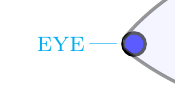
\begin{tikzpicture}
		\path node (eye) at (0.1,0) [shape=circle,draw,fill=blue!900,opacity=1,very thick,inner sep=0.1cm,label={[label distance=-2pt]left:{\textcolor{cyan}{\textsc{eye}\thinspace---}}}] {};
		\draw [very thick,overlay,fill=blue!10,opacity=0.4] (-.04,0.06) arc (140:90:3cm) arc (90:-90:1cm) arc (-90:-129:3.64cm);  
		\end{tikzpicture}
	\end{center}
}

\frame{{How to generate \textcolor{red}{pseudo-profound bullshit}?}\vspace{-3pt}
	\begin{enumerate}\setcounter{enumi}{4}
		\item \textcolor{blue}{use jargon.}
		\begin{itemize}
			\item The Nothing itself nothings.
			\item Profound boredom, drifting here and there in the abysses of our existence like a muffling fog, removes all things and men and oneself along with it into a remarkable indifference. This boredom reveals being as a whole.
			\item Dasein has always made some sort of decision as to  the way in which it is in each case mine. That entity which in its Being has this very Being as an issue, comports itself towards its Being as its ownmost possibility. With death, Dasein stands before itself in its ownmost potentiality-for-Being.
			\item The Absolute Idea. The Idea, as unity of the Subjective and Objective Idea, is the notion of the Idea --- a notion whose object  is the Idea as such, and for which the objective is Idea --- an Object which embraces all characteristics in its unity.
			\item A machinic assemblage, through its diverse components, extracts its consistency by crossing ontological thresholds, non-linear thresholds of irreversibility, ontological and phylogenetic thresholds, creative thresholds of heterogenesis and autopoiesis.
		\end{itemize}
	\end{enumerate}
}

\frame{{The Unreasonable Ineffectiveness of Philosophy}
	\begin{tcolorbox}\small
		\begin{itemize}
			\item 费曼:“砖头算不算本质客体?”
			\item 哲学家甲:“一块砖是独特的砖,是怀海德所说的本质客体。” 
			\item 哲学家乙:“本质客体的意思并不是指个别的砖块,而是指所有砖块的共有的普遍性质,换句话说,‘砖性’才是本质客体。”
			\item 哲学家丙:“不对,重点不在砖本身,‘本质客体’指的是,当你想到砖块时内心形成的概念。”
			\item 就像所有关于哲学家的故事一样,最终以一片混乱收场。好笑的是,在先前的那么多次讨论中,他们从来没有问过自己,像简单的砖块究竟是不是“本质客体”。
			\item 科学哲学对科学家的用处跟鸟类学对鸟的用处差不多。\hfill --- {\sl 费曼}
		\end{itemize}
	\end{tcolorbox}
\begin{itemize}
	\item 哲学旨在感动那些混淆晦涩与深刻的人。 \hfill --- {\sl 温伯格}
	\item 哲学难道不是用蜜写成的吗?乍一看,很精彩,再一看,除了一团浆糊,什么都没留下。 \hfill --- {\sl 爱因斯坦}
\end{itemize}
}

\frame{{The Unreasonable Ineffectiveness of Philosophy}
	\begin{itemize}
		\item When a philosopher says something that is true then it is trivial. When he says something that is not trivial then it is false.\hfill --- \sl Gauss
		\item There is only one thing a philosopher can be relied upon to do, and that is to contradict other philosophers.\hfill --- \sl James
		\item Philosophers are free to do whatever they please, because they don't have to do anything right.
		\item Philosophy is to science as pornography is to sex: it is cheaper, easier, and some people seem, bafflingly, to prefer it.
		\item A philosopher looking for the ultimate truth is like a blind darky with an extinguished candle on a dark night searching a dark subterranean cave for a black cat that isn't there, and shouting ``I found it!''
	\end{itemize}
}

\frame{{Elimination of Metaphysics\textcolor{red}{?$\times$?}}
	\begin{tcolorbox}\small
		一个陈述的意义在于它的\textcolor{red}{证实方法}。形而上学陈述不能被证实,毫无意义。那么留给哲学的还有什么呢?一种方法:逻辑分析法。逻辑分析的消极应用是清除无意义的词和陈述,积极应用是澄清有意义的概念和命题,为经验科学和数学奠基。形而上学家相信自己是在攸关\textcolor{red}{真假}的领域里前行,却未断言任何东西。他们只是试图表达一点儿人生态度。艺术是表达人生态度的恰当手段。抒情诗人并不企图在自己的诗里驳倒其他抒情诗人诗里的陈述,但形而上学家却用论证维护他的陈述。形而上学家是没有艺术才能的艺术家,有的是在理论环境里工作的爱好,却既不在科学领域里发挥这种爱好,又不能满足艺术表达的要求,倒是混淆了这两个方面,创造出一种对知识既无贡献、对人生态度的表达又不相宜的东西。\footnote{卡尔纳普:通过语言的逻辑分析清除形而上学}
	\end{tcolorbox}
			Mystics exult in mystery and want it to stay mysterious. Scientists exult in mystery for a different reason: it gives them something to do.\par
			\hfill --- \sl Dawkins
}

\frame{{Practice is the sole criterion for testing truth?}
\centering\fbox{Practice is the sole criterion for testing truth?}
	\begin{columns}[onlytextwidth]
		\column{0.57\textwidth}
				\begin{itemize}
					\item What is ``practice''?
					\item What is ``truth''?
					\item What is ``criterion''?
					\item Why ``sole'' criterion?
					\item How to ``test''?
					\item How to test ``truth'' with ``practice''?
				\end{itemize}
		\column{0.43\textwidth}
			\begin{figure}
				\includegraphics[width=\textwidth]{img/test.jpg}
			\end{figure}
	\end{columns}
}

\frame{{Galilei's Leaning Tower of Pisa}
	\begin{columns}[onlytextwidth]
	\column{.4\textwidth}
	\begin{figure}
	\includegraphics[width=\textwidth]{img/tower-pisa.jpg}
	\end{figure}
	\column{.6\textwidth}
		\begin{quote}\sl
			\emph{\texttt{Philosophy is written in this grand book --- I mean the universe --- which stands continually open to our gaze, but it can't be understood unless one first learns to comprehend the language in which it is written. It is written in the language of mathematics.}}\\\hfill --- {\texttt{Galileo Galilei}}
		\end{quote}
	\end{columns}
}

\frame{{Why is the Night Sky Dark?}
\begin{columns}[onlytextwidth]
		\column{0.5\textwidth}
			\begin{center}
				\begin{figure}
					\includegraphics[width=\textwidth]{img/dark-sky}
				\end{figure}
			\end{center}
		\begin{tcolorbox}
		A \textcolor{red}{static}, \textcolor{red}{infinitely old} universe with an \textcolor{red}{infinite number} of stars \textcolor{red}{uniformly distributed} in an \textcolor{red}{infinitely large space} would be bright rather than dark.
		\end{tcolorbox}
		\column{0.5\textwidth}\vspace{-2ex}
			\begin{center}
				\begin{figure}
				\begin{overpic}[scale=0.27]{img/poe.jpg}
				\put(2,95){\textcolor{fore}{\footnotesize 星若无穷尽,天空将明亮。}}
				\put(2,88){\textcolor{fore}{\footnotesize 仰望银河,君可见背景片片无点状?}}
				\put(2,81){\textcolor{fore}{\footnotesize 夜空暗黑,原因此一桩。}}
				\put(2,74){\textcolor{fore}{\footnotesize 光行万里,发于恒星之初创。}}
				\put(2,67){\textcolor{fore}{\footnotesize 抵达地球未及时,只因路遥道太长。}}
			\end{overpic}
				\end{figure}
			\end{center}
\end{columns}
}

\frame{{Newton's Apple}
\centering\fbox{If an apple falls, does the moon also fall?}
	\begin{columns}[onlytextwidth]
		\column{0.55\textwidth}
				\begin{itemize}
					\item What is ``rest/motion''?
					\item What is ``state of rest/motion''?
					\item What is ``change/tends to change''?
					\item What is ``body''?
					\item What is ``force''?
					\item What is ``definition''?
				\end{itemize}
		\column{0.33\textwidth}
			\begin{overpic}[scale=0.2]{img/applenewton.jpg}
			\put(1,57){$F=\frac{Gm_1m_2}{r^2}$}
			\put(1,92){$F=0\Rightarrow v=c$}
			\put(1,84){$F=ma$}
			\put(1,74){$F_{12}=-F_{21}$}
			\end{overpic}
	\end{columns}
\centering\boxed{\vbox{A force is that which changes or tends to change the state of rest or motion of a body.}}
}

\frame{{Einstein's Train Thought Experiment}
\begin{figure}
	\includegraphics[width=.6\textwidth]{img/simultaneity}
\end{figure}
\begin{itemize}
	\item What is ``simultaneity''?
	\item How to measure ``simultaneity''?
	\item How to measure ``time''?
\end{itemize}
}

\frame{{Einstein's Elevator Thought Experiment}
	\begin{columns}\hspace{-9pt}
		\column{0.64\textwidth}
			\begin{itemize}
				\item The gravitational ``force'' as experienced locally while standing on a massive body is actually the same as the pseudo-force experienced by an observer in a non-inertial (accelerated) frame of reference.
				\item Spacetime tells matter how to move; matter tells spacetime how to curve.
				\item Gravity is not a force that applies via Newton's $2^{nd}$ Law, but a consequence of the curvature of spacetime caused by the uneven distribution of mass/energy that acts via the geodesic principle, which is the relativistic equivalent of Newton's $1^{st}$ Law.
			\end{itemize}
		\column{0.4\textwidth}\vspace{-5pt}
			\begin{figure}
				\includegraphics[width=.57\textwidth]{img/grav.pdf}
				\includegraphics[width=.4\textwidth]{img/acc.pdf}
			\end{figure}
			\begin{figure}
				\includegraphics[width=\textwidth]{img/spacetime-curvature.png}
			\end{figure}
	\end{columns}
}

\frame{{Logic of Science}
	\begin{tcolorbox}
		\begin{center}
			\textbf{\large{How to \textcolor{red}{\textit{express}} your thoughts \underline{precisely} and \underline{succinctly}?}}
		\end{center}
	\end{tcolorbox}
	\begin{itemize}
		\item Not only is the universe stranger than we imagine, it is stranger than we can imagine.
		\item A few lines of \textcolor{red}{reasoning} can change the way we see the world.
		\item Logic enlarges our abstract imagination, and provides all possible hypotheses to be applied in the analysis of complex facts. Nothing is forbidden except nonsense and contradiction.
		\item Logic is the immune system of the mind!
		\item The music of reason --- the fulfillment of the human spirit.
	\end{itemize}
}

\frame{{The Music of Reason}
	\begin{center}
		\large{\textcolor{red}{\textbf{How to \textit{express} your thoughts \underline{precisely} and \underline{succinctly}?}}}
	\end{center}
	\begin{figure}
		\includegraphics[width=0.9\textwidth]{img/music.png}
	\end{figure}
	\begin{center}
	The glory of the human spirit!\\
	\large{\textcolor{red}{What are the extent and limits of reason?}}
	\end{center}
}

%%%%%%%%%%%%%%%%%%%%%%%%%%%%%
\subsection{Logic and other Disciplines}
%%%%%%%%%%%%%%%%%%%%%%%%%%%%%

\frame{{Why Study Logic?}
		\begin{itemize}
			\item Logic vs (Analytic) Philosophy.
			
			sense \& reference / extension \& intension / use \& mention / truth \& provability / mutual vs distributed vs common knowledge / knowledge update / belief revision / preference change / information flow / action \& strategy / multi-agent interaction / counterfactual / causation / possible world / cross-world identity / essentialism / induction / ontological commitment / concept analysis / laws of thought / strength \& limitation / paradoxes \dots
			
			Peirce, Frege, Russell, Wittgenstein, Ramsey, Carnap, Quine, Putnam, Kripke, Chomsky, G\"odel, Tarski, Turing \dots
			\item Logic vs Mathematical Foundations.
			
			Logicism / Formalism / Intuitionism / Constructivism / Finitism / Structuralism / \href{https://homotopytypetheory.org/book/}{Homotopy Type Theory}
			\item Logic vs Computer Science.
			\[\dfrac{\text{Logic}}{\text{Computer Science}} \approx \dfrac{\text{Calculus}}{\text{Physics}}\]
			\item $\cdots$
		\end{itemize}
}

\frame{{Logic vs CS}
	\begin{itemize}
		\item Computer Architecture.
		
		Gates and digital circuit design $\approx$ Propositional Logic
		\item Programming Languages.
		
		Semantics of programming languages via methods of logic\\
		LISP $\approx$ $\lambda$-calculus\\
		Prolog $\approx$ First Order Logic $+$ Recursion\\
		Typing $\approx$ Type Theory
		\item Theory of Computation and Computational Complexity.
		
		Models of computation (Turing machines, finite automata)\\
		Logic provides \emph{complete problems} for complexity classes.\\
		Logical characterizations of complexity classes\\
		Descriptive Complexity
		\item  Theorem Proving
	\end{itemize}
}

\frame{{Logic vs CS}
	\begin{itemize}
		\item Knowledge representation via logic rules
		\item Common sense reasoning via Non-monotonic Logic
		\item Fuzzy Control vs Fuzzy Logic and Multi-valued Logic
		\item Relational Databases
		
		SQL $\approx$ First Order Logic $+$ Syntactic Sugar
		\item Hardware and Software Verification.
		
		Extensive use of formal methods based on logic\\
		Temporal Logic, Dynamic Logic and Automata, Hoare Logic, Model Checking
		\item Agents.
		
		Epistemic Logic
		\item Semantic Web.
		
		Web Ontology Language (OWL) $\approx$ Description Logic
	\end{itemize}
}

\frame[shrink]{{Branches of Logic}\vspace{-2pt}
	\resizebox{\textwidth}{!}{
		\begin{minipage}{13cm}
			\begin{columns}
				\column{0.33\textwidth}
					\centering\textcolor{red}{\underline{\textbf{Mathematical Logic}}}
				\column{0.37\textwidth}
					\centering\textcolor{red}{\underline{\textbf{Computational Logic}}}
				\column{0.33\textwidth}
					\centering\textcolor{red}{\underline{\textbf{Philosophical Logic}}}
			\end{columns}\vspace{-1ex}
			\begin{columns}
				\column{0.34\textwidth}
					\begin{itemize}
						\item \colorbox{black}{\textbf{\textcolor{fore}{First Order Logic}}}
						\item  \textcolor{darkgreen}{Set Theory}
						\item \textcolor{darkgreen}{Model Theory}
						\item \textcolor{darkgreen}{Proof Theory}
						\item \textcolor{darkgreen}{Recursion Theory}
					\end{itemize}
				\column{0.39\textwidth}
					\begin{itemize}
						\item \textcolor{darkgreen}{Automata Theory}
						\item \textcolor{darkgreen}{Computational Complexity}
						\item \textcolor{darkgreen}{Finite Model Theory}
						\item \textcolor{darkgreen}{Model Checking}
						\item \textcolor{darkgreen}{Type Theory}
						\item \textcolor{darkgreen}{Lambda Calculus}
						\item \textcolor{darkgreen}{Categorical Logic}
						\item \textcolor{darkgreen}{Theorem Proving}
						\item Description Logic
						\item Dynamic Logic
						\item Temporal Logic
						\item Hoare Logic
						\item Inductive Logic
						\item Fuzzy Logic
						\item Non-monotonic Logic
						\item Computability Logic
						\item Default Logic
						\item Situation Calculus
					\end{itemize}
				\column{0.34\textwidth}
					\begin{itemize}
						\item \textcolor{darkgreen}{Intuitionistic Logic}
						\item \textcolor{darkgreen}{Algebraic Logic}
						\item \textcolor{darkgreen}{Quantum Logic}
						\item \textcolor{blue}{Modal Logic}
						\item Epistemic Logic
						\item Doxastic Logic
						\item Preference Logic
						\item Provability Logic
						\item Hybrid Logic
						\item Free Logic
						\item Conditional Logic
						\item Relevance Logic
						\item Linear Logic
						\item Paraconsistent Logic
						\item Intensional Logic
						\item Partial Logic
						\item Diagrammatic Logic
						\item Deontic Logic
					\end{itemize}
			\end{columns}
	\end{minipage}}
}

\frame{{$\nabla(\odot\!\cdot\!\odot)=\mathop{\odot\nabla\odot}+\mathop{\odot\nabla\odot}$}
\begin{columns}
\column{.65\textwidth}
	\Large{
		\begin{itemize}
			\item Logic is
			\begin{enumerate}
				\item mainly philosophy by subject matter
				\item mainly mathematics by methodology
				\item mainly computer science by applications
			\end{enumerate}
			\item  Logicians always want to be
			\begin{enumerate}
				\item Philosophers of philosophers
				\item Mathematicians of mathematicians
				\item Computer scientists of computer scientists
			\end{enumerate}
			\item However, they often end up being
			\begin{enumerate}
				\item Mathematicians to philosophers
				\item Computer scientists to mathematicians
				\item Philosophers to computer scientists
			\end{enumerate}
	\end{itemize}}
\column{.43\textwidth}
				\begin{center}
					\begin{tikzpicture}[scale=0.45]
					\draw[back, very thick](6,2.5)circle(3 and 3)node(C){${\textbf{CS}}\atop{\textit{\textcolor{black}{useful}}}$};
					\draw[back, very thick](8,6)circle(3 and 3)node(P){${\textbf{Philo}}\atop{\textit{\textcolor{black}{to the point}}}$};
					\draw[back, very thick](10,2.5)circle(3 and 3)node(M){${\textbf{Math}}\atop{\textit{\textcolor{black}{rigid}}}$};
					\begin{scope}
					\clip(8,6)circle(3 and 3);
					\clip(10,2.5)circle(3 and 3);
					\clip(6,2.5)circle(3 and 3);
					\filldraw[back,fill=gray,nearly transparent,opacity=.5](0,0)rectangle(10,5);
					\end{scope}
					\node at ($0.33*(C)+0.33*(M)+0.33*(P)$){$\textcolor{red}{\textbf{L}}$};
					\end{tikzpicture}
				\end{center}
\end{columns}
}

\frame{{}
\begin{quote}
Between theology and science there is a no man's land, exposed to attack from both sides; this no man's land is philosophy.\par\hfill --- {\sl Russell}
\end{quote}
\begin{quote}
Philosophy is a `catalyst' or `spice' which makes the interdisciplinary mixture work. `Philosophy-internal' issues seem like intellectual black holes: they absorb a lot of clever energy, but nothing ever seems to come out.\par\hfill --- {\sl van Benthem}
\end{quote}
	\begin{itemize}
		\item Philosophy is a game with objectives and no rules.
		\item Logic is a game with rules and no objectives. 
	\end{itemize}
	\begin{block}{Logic is like love; a simple idea, but it can get complicated.}
		\begin{itemize}
			\item 这TM也用证?
			\item 这TM也能证?
		\end{itemize}
	\end{block}
	\begin{quote}
		If Church says it's obvious, then everybody has seen it half an hour ago. If Weyl says it's obvious, von Neumann might be able to prove it. If Lefschetz says it's obvious, it's false.\par\hfill --- {\sl Rosser}
	\end{quote}
}

%%%%%%%%%%%%%%%%%%%%%%%%%%%%%%%%
\section{History}
%%%%%%%%%%%%%%%%%%%%%%%%%%%%%%%%

%------------------------------------%
\subsection{The Prehistory of Logic}
%------------------------------------%

\frame{{Aristotle(384-322 BC) --- Term Logic}
	\begin{columns}
		\column{0.7\textwidth}
			\begin{itemize}
				\item Term Logic.
				\item Aristotle believed that any logical argument can, in principle, be broken down into a series of applications of a small number of syllogisms.
				\item Any person in the present day who wishes to learn logic will be wasting his time if he reads Aristotle.\\
				\hfill --- {\sl Russell}
			\end{itemize}
		\column{0.2\textwidth}
			\begin{figure}
				\includegraphics[width=\textwidth]{img/aristotle.jpg}
			\end{figure}
	\end{columns}
}

{\setbeamercolor{normal text}{bg=white}
	\frame{{Sophistic vs Valid Argument}
		\begin{columns}
			\column{.32\textwidth}{\small
					\begin{enumerate}
						\item 没有东西存在;
						\item 就算有东西存在,也无法认识它;
						\item 就算能认识它,也无法与他人谈论它;
						\item 就算能谈论它,也无法互相理解。
				\end{enumerate}}
				\begin{prooftree}
					\AxiomC{All men are mortal}
					\noLine
					\UnaryInfC{Socrates is a man}
					\alwaysSingleLine
					\UnaryInfC{Socrates is mortal}
				\end{prooftree}
			\column{.6\textwidth}
				\begin{tabu}{m{3.4cm} m{1.9cm}  @{}m{0pt}@{}}
					\textbf{A}: All $S$ are $P$.&
					\begin{tikzpicture}[scale=0.3]
					\begin{scope}
					\clip(6,2.5)circle(3 and 3);
					%\clip(8,6)circle(3 and 3);
					%\clip(10,2.5)circle(3 and 3);
					\filldraw[back,fill=gray,nearly transparent,opacity=0.7](0,-2)rectangle(20,10);
					\end{scope}
					\begin{scope}
					%\clip(6,2.5)circle(3 and 3);
					%\clip(8,6)circle(3 and 3);
					\clip(10,2.5)circle(3 and 3);
					\filldraw[back,fill=white!30,opacity=1](0,-2)rectangle(20,10);
					\end{scope}
					\draw[back, very thick](6,2.5)circle(3 and 3)node(S){S};
					\draw[back, very thick](10,2.5)circle(3 and 3)node(P){P};
					\node at ($0.5*(S)+0.5*(P)$){\huge $\textcolor{red}{\circledtimes}$};
					\end{tikzpicture}\\
					\textbf{E}: No $S$ are $P$. &
					\begin{tikzpicture}[scale=0.3]
					\begin{scope}
					\clip(6,2.5)circle(3 and 3);
					%\clip(8,6)circle(3 and 3);
					\clip(10,2.5)circle(3 and 3);
					\filldraw[back,fill=gray,nearly transparent,opacity=0.7](0,-2)rectangle(20,10);
					\end{scope}
					\draw[back, very thick](6,2.5)circle(3 and 3)node(S){S};
					\draw[back, very thick](10,2.5)circle(3 and 3)node(P){P};
					\node at ($0.85*(S)+0.001*(P)$){\huge $\textcolor{red}{\circledtimes}$};
					\end{tikzpicture}\\
					\textbf{I}: Some $S$ are $P$. &
					\begin{tikzpicture}[scale=0.3]
					\draw[back, very thick](6,2.5)circle(3 and 3)node(S){S};
					\draw[back, very thick](10,2.5)circle(3 and 3)node(P){P};
					\node at ($0.5*(S)+0.5*(P)$){\huge $\textcolor{red}{\times}$};
					\end{tikzpicture}\\
					\textbf{O}: Some $S$ are not $P$. &
					\begin{tikzpicture}[scale=0.3]
					\draw[back, very thick](6,2.5)circle(3 and 3)node(S){S};
					\draw[back, very thick](10,2.5)circle(3 and 3)node(P){P};
					\node at ($0.85*(S)+0.001*(P)$){\huge $\textcolor{red}{\times}$};
					\end{tikzpicture}
				\end{tabu}
		\end{columns}
	}
}

{\setbeamercolor{normal text}{bg=white}
	\frame{{Syllogism}
		\begin{columns}
			\column{0.25\textwidth}
				\begin{prooftree}
					\AxiomC{$M$---$P$}
					\noLine
					\UnaryInfC{$S$---$M$}
					\alwaysSingleLine
					\UnaryInfC{$S$---$P$}
				\end{prooftree}
			\column{0.25\textwidth}
				\begin{prooftree}
					\AxiomC{$P$---$M$}
					\noLine
					\UnaryInfC{$S$---$M$}
					\alwaysSingleLine
					\UnaryInfC{$S$---$P$}
				\end{prooftree}
			\column{0.25\textwidth}
				\begin{prooftree}
					\AxiomC{$M$---$P$}
					\noLine
					\UnaryInfC{$M$---$S$}
					\alwaysSingleLine
					\UnaryInfC{$S$---$P$}
				\end{prooftree}
			\column{0.25\textwidth}
				\begin{prooftree}
					\AxiomC{$P$---$M$}
					\noLine
					\UnaryInfC{$M$---$S$}
					\alwaysSingleLine
					\UnaryInfC{$S$---$P$}
				\end{prooftree}
		\end{columns}
		\begin{columns}
			\column{0.4\textwidth}
				\begin{itemize}
					\item 大项:结论的谓项。
					\item 小项:结论的主项。
					\item 中项:第三个项。
				\end{itemize}
				\begin{itemize}
					\item 大前提:含大项的前提。
					\item 小前提:含小项的前提。
				\end{itemize}
			\column{0.6\textwidth}
				\begin{center}
					\begin{itemize}
						\item 4格,$4^3\times 4=256$式。
						\item $15$布尔有效式。
						\item $24$亚里士多德有效式。 \textcolor{red}{(存在预设)}
						\item 如何断定三段论的有效性?
						\begin{enumerate}
							\item \textcolor{blue}{Venn Diagrams}
							\item \textcolor{blue}{Rules}
							\item \textcolor{darkgreen}{Boolean Algebra}
							\item \colorbox{yellow}{\textcolor{black}{Axiomatization}}
						\end{enumerate}
					\end{itemize}
				\end{center}
		\end{columns}
	}
}

{\setbeamercolor{normal text}{bg=white}
	\frame{{Venn Diagram --- Boolean Standpoint}
		\begin{columns}
			\column{0.6\textwidth}
				\begin{enumerate}
					\item 在三个圆的图上标记三段论的三个项;
					\item 把两个前提在图上表示出来,如果一个前提是全称、另一个是特称,先表示全称;
					\item 如果特称前提没有明确表明把 \textcolor{red}{$\times$} 画在哪一部分,就把它画在交叉线上;
					\item 检查图示是否支持结论。
				\end{enumerate}
			\column{0.4\textwidth}
				\begin{prooftree}
					\AxiomC{No $P$ are $M$}
					\noLine
					\UnaryInfC{Some $S$ are not $M$}
					\alwaysSingleLine
					\UnaryInfC{Some $S$ are $P$}
				\end{prooftree}
				\begin{center}
					\begin{tikzpicture}[scale=0.5]
					\draw[back, very thick](6,2.5)circle(3 and 3)node(S){S};
					\draw[back, very thick](8,6)circle(3 and 3)node(M){M};
					\draw[back, very thick](10,2.5)circle(3 and 3)node(P){P};
					\begin{scope}
					%\clip(6,2.5)circle(3 and 3);
					\clip(8,6)circle(3 and 3);
					\clip(10,2.5)circle(3 and 3);
					\filldraw[back,fill=gray,nearly transparent,opacity=0.7](0,0)rectangle(20,10);
					\end{scope}
					%\node at ($0.33*(S)+0.33*(M)+0.33*(P)$){};
					\node at ($0.665*(S)+0.3*(P)$){\huge $\textcolor{red}{\times}$};
					\end{tikzpicture}
				\end{center}
		\end{columns}
	}
}

{\setbeamercolor{normal text}{bg=white}
	\frame{{Venn Diagram --- Aristotelean Standpoint}
		\begin{columns}
			\column{0.6\textwidth}
				\begin{enumerate}
					\item 如果一个含全称前提和特称结论的三段论形式不是布尔有效的,看看是否有一个圆其中除了一个区域外全是阴影,如果有,在那个区域画 \textcolor{red}{$\bigotimes$} 。
					\item 如果该三段论是条件有效的,检查 \textcolor{red}{$\bigotimes$} 是否表示某个存在物,如果是,则该三段论是亚里士多德有效的。
				\end{enumerate}
			\column{0.4\textwidth}
				\begin{prooftree}
					\AxiomC{No $M$ are $P$}
					\noLine
					\UnaryInfC{All $M$ are $S$}
					\alwaysSingleLine
					\UnaryInfC{Some $S$ are not $P$}
				\end{prooftree}
				\begin{center}
					\begin{tikzpicture}[scale=0.5]
					\begin{scope}
					%\clip(6,2.5)circle(3 and 3);
					\clip(8,6)circle(3 and 3);
					\clip(10,2.5)circle(3 and 3);
					\filldraw[back,fill=blue!30,opacity=0](0,0)rectangle(20,10);
					\end{scope}
					
					\begin{scope}
					%\clip(6,2.5)circle(3 and 3);
					\clip(8,6)circle(3 and 3);
					%\clip(10,2.5)circle(3 and 3);
					\filldraw[back,fill=gray,nearly transparent,opacity=0.7](0,0) rectangle (41,41);
					\end{scope}
					
					\begin{scope}
					\clip(6,2.5)circle(3 and 3);
					%\clip(8,6)circle(3 and 3);
					%\clip(10,2.5)circle(3 and 3);
					\filldraw[back,fill=white!30,opacity=1](0,-3)rectangle(30,20);
					\end{scope}
					
					\begin{scope}
					%\clip(6,2.5)circle(3 and 3);
					\clip(8,6)circle(3 and 3);
					\clip(10,2.5)circle(3 and 3);
					\filldraw[back,fill=gray,nearly transparent,opacity=0.7](0,0)rectangle(20,10);
					\end{scope}

					\draw[back, very thick](6,2.5)circle(3 and 3)node(S){S};
					\draw[back, very thick](8,6)circle(3 and 3)node(M){M};
					\draw[back, very thick](10,2.5)circle(3 and 3)node(P){P};
					
					%\node at ($0.33*(S)+0.33*(M)+0.33*(P)$){};
					\node at (6.7,4.5){\huge $\textcolor{red}{\circledtimes}$};
					\end{tikzpicture}
				\end{center}
		\end{columns}
	}
}

{\setbeamercolor{normal text}{bg=white}
	\frame{{三段论有效性的判定规则}\vspace{-12pt}
		\begin{center}
			\renewcommand\arraystretch{2}
			\vbox{\begin{tabu}{r !{\vrule width2pt} l !{\vrule width2pt} l !{\vrule width2pt}l}
					\multicolumn{1}{r}{}& \multicolumn{2}{c}{\textcolor{blue}{$S$ 周延}}&\multicolumn{1}{l}{}\\
					\Xcline{2-3}{2pt}
					\multirow{2}{*}[-0ex]{\textcolor{blue}{\!\!\!\!$P$ 不周延}}&\textcolor{red}{\textbf{A}: \underline{All} $S$ are $P$.} &\textcolor{red}{\textbf{E}: \underline{No} $S$ are $P$.} & \multirow{2}{*}[-0ex]{\textcolor{blue}{$P$ 周延}}\\
					\Xcline{2-3}{2pt}
					&\textcolor{red}{\textbf{I}: Some $S$ are $P$.}  &\textcolor{red}{\textbf{O}: Some $S$ are \underline{not} $P$.} &\\
					\Xcline{2-3}{2pt}
					\multicolumn{1}{c}{}& \multicolumn{2}{c}{\textcolor{blue}{$S$ 不周延}}&
			\end{tabu}}\vspace{-5pt}
		\end{center}
		\begin{enumerate}
			\item 中项至少周延一次。
			\item 结论中周延的项在前提中必周延。
			\item 前提与结论中否定命题的数目必相同。
			\item 特称结论需要特称前提。 \quad\textcolor{red}{(存在谬误)}\vspace{-2.7cm}
			\[\textcolor{red}{\left.\phantom{aaaaaaabbbbbbbb+\dfrac{\dfrac{2}{3}}{\dfrac{a}{b}}}\right\}\; Aristotle}\]\vspace{-2.1cm}
			\[\textcolor{red}{\left.\phantom{aaaaaaaaaaaaaaaaaaaaaaaaaabbbbbbbbbb+\dfrac{\frac{2}{3}}{\dfrac{\frac{2}{3}}{\frac{2}{3}}}}\right\}\; Boole}\]
		\end{enumerate}
	}
}	

\frame{{Example and Criticism}
	\begin{columns}
		\column{0.5\textwidth}
			\begin{prooftree}
				\AxiomC{All men are intelligent}
				\noLine
				\UnaryInfC{Women are not men}
				\alwaysSingleLine
				\UnaryInfC{Women are not intelligent}
			\end{prooftree}
			\begin{prooftree}
				\AxiomC{John does not read books}
				\noLine
				\UnaryInfC{Students who like to learn read books}
				\alwaysSingleLine
				\UnaryInfC{John does not like to learn}
			\end{prooftree}
			\begin{prooftree}
				\AxiomC{Nothing is better than money}
				\noLine
				\UnaryInfC{Philosophy is better than nothing}
				\alwaysSingleLine
				\UnaryInfC{Philosophy is better than money}
			\end{prooftree}
		\column{0.5\textwidth}
			\begin{prooftree}
				\AxiomC{Only man is rational}
				\noLine
				\UnaryInfC{No woman is a man}
				\alwaysSingleLine
				\UnaryInfC{No woman is rational}
			\end{prooftree}
			\begin{prooftree}
				\AxiomC{No professors are ignorant}
				\noLine
				\UnaryInfC{All ignorant people are vain}
				\alwaysSingleLine
				\UnaryInfC{No professors are vain}
			\end{prooftree}
			\begin{prooftree}
				\AxiomC{Everyone loves my baby}
				\noLine
				\UnaryInfC{My baby loves only me}
				\alwaysSingleLine
				\UnaryInfC{I am my own baby}
			\end{prooftree}
	\end{columns}
}

\frame{{Deduction/Induction/Abduction/Examplification}
	\begin{prooftree}
		\AxiomC{$M\to P$}
		\noLine
		\UnaryInfC{$S\to M$}
		\alwaysSingleLine
		\UnaryInfC{$S\to P$}
	\end{prooftree}
	\begin{prooftree}
		\AxiomC{$M\to P$}
		\noLine
		\UnaryInfC{$M\to S$}
		\alwaysSingleLine
		\UnaryInfC{$S\to P$}
	\end{prooftree}
	\begin{columns}
		\column{0.33\textwidth}
			\begin{prooftree}
				\AxiomC{$H\to E$}
				\noLine
				\UnaryInfC{$\phantom{H\to} E$}
				\alwaysSingleLine
				\UnaryInfC{$H$}
			\end{prooftree}
		\column{0.33\textwidth}
			\begin{prooftree}
				\AxiomC{$P\to M$}
				\noLine
				\UnaryInfC{$S\to M$}
				\alwaysSingleLine
				\UnaryInfC{$S\to P$}
			\end{prooftree}
		\column{0.33\textwidth}
			\begin{prooftree}
				\AxiomC{$H\to E$}
				\noLine
				\UnaryInfC{$\top\to E$}
				\alwaysSingleLine
				\UnaryInfC{$\top\to H$}
			\end{prooftree}
	\end{columns}
	\begin{prooftree}
		\AxiomC{$P\to M$}
		\noLine
		\UnaryInfC{$M\to S$}
		\alwaysSingleLine
		\UnaryInfC{$S\to P$}
	\end{prooftree}
}

\frame{{Abduction}
\begin{tcolorbox}
\begin{enumerate}
	\item 观察到恒星光谱红移。
	\item 如果恒星在退行,那么恒星光谱红移就可以解释。
	\item 如果整个宇宙在膨胀,那么恒星在离我们而去。
	\item 如果宇宙起源于大爆炸,那么宇宙就会膨胀。
	\item 因此,宇宙起源于大爆炸。
\end{enumerate}
\end{tcolorbox}
	\begin{figure}
		\includegraphics[width=0.25\textwidth,angle=0,origin=c]{img/conan}
	\end{figure}
}

\frame{{Leibniz 1646-1716}
	\begin{columns}
		\column{0.43\textwidth}
			\begin{figure}
				\includegraphics[width=\textwidth,angle=0,origin=c]{img/leibniz0.jpg}
			\end{figure}
		\column{0.57\textwidth}
			\begin{tcolorbox}[colback=cyan!3,colframe=back!85]
				\centerline{\Large Don't argue. Calculate!}
			\end{tcolorbox}
			\begin{itemize}
				\item \textcolor{red}{{\small Principle of Contradiction}}: Nothing can be and not be, but everything either is or is not.
				\item \textcolor{red}{{\small Principle of Sufficient Reason}}: Nothing is without a reason.
				\item \textcolor{blue}{{\small Principle of Perfection}}: The real world is the best of all possible worlds.
			\end{itemize}
			\begin{alertblock}{In the beginning was the Logic.}
				As God calculates, so the world is made.
			\end{alertblock}
	\end{columns}
}

\frame{{Leibniz}
	\begin{itemize}
		\item The last ``universal genius'', developed Calculus, refined binary number system, invented mechanical calculator that could perform addition, subtraction, multiplication and division.
		\item Leibniz was claimed (by Russell, Euler, G\"odel, Weiner, Mandelbrot, Robinson, Chaitin) to be a precursor of \emph{mathematical logic, topology, game theory, cybernetic theory, fractal geometry, non-standard analysis, algorithmic information theory and digital philosophy}.
		\item Wolfram: ``Leibniz had the idea of encoding logical properties using numbers. He thought about associating every possible attribute of a thing with a prime number, then characterizing the thing by the product of the primes for its attributes --- and then representing logical inference by arithmetic operations.''
		%\item Diderot: ``When one compares the talents one has with those of a Leibniz, one is tempted to throw away one's books and go die quietly in the dark of some forgotten corner.''
	\end{itemize}
}

{\setbeamercolor{normal text}{fg=fore,bg=back}\usebeamercolor[fg]{normal text}
	\frame{{Leibniz's Dream --- Deduction}
		\begin{enumerate}[1]
			\item \emph{Universal Characteristic and Rational Calculus.}
			\begin{enumerate}[i]
				\item \textcolor{green}{encyclopedia} --- arranged in a logical order according to a demonstrative method, beginning with definitions of all the simple and primitive terms (which form the alphabet of human thoughts).
				\item a \textcolor{green}{universal ideal language} that is purged of ambiguity and vagueness. \textit{--- the language of creation, the language before the Tower of Babel, the language that God used in creating the universe, the language whose  rules of composition directly expresses the structure of the universe, the language in which concepts are expressed in their direct, original format.%\vspace{-1pt}
					\[\textcolor{orange}{\text{sign}\rightleftarrows\text{idea}}\]
					\begin{center}
						{\footnotesize \textcolor{brown}{
								encyclopedia $\Rightarrow$ fundamental principles $\Rightarrow$ primitive notions}}
				\end{center}}
				\item the arrangement of \textcolor{green}{all true propositions} in an \textcolor{green}{axiomatic system}.
				\item \textcolor{green}{decision procedure}. A calculus of manipulating the knowledge in a computational fashion, so as to reveal its logical interrelations and consequences. \textcolor{cyan}{--- replace reasoning by computation.}
				\item a proof that the rational calculus is \textcolor{green}{consistent}.
				\item a procedure for the rapid enlargement of knowledge. \textcolor{cyan}{--- the art of invention. free mind from intuition.}
			\end{enumerate}
		\end{enumerate}
	}
	
	\frame{{\href{https://philpapers.org/rec/HACTLP}{\textcolor{fore}{Leibniz's Dream --- Induction}}}
		\begin{figure}
			\colorbox{white}{\includegraphics[width=0.23\textwidth,angle=0,origin=c]{img/overfitting}}
		\end{figure}
		\vspace{-7pt}
		\begin{enumerate}\setcounter{enumi}{1}
			\item \emph{Compute all descriptions of possible worlds that can be expressed with the primitive notions. And the possible worlds will all have some propensity to exist.}
			\item \emph{Compute the probabilities of disputed hypotheses relative to the available data. As we learn more our probability assignments will asymptotically tend to a maximum for the real world, i.e., the possibility with the highest actual propensity.}
		\end{enumerate}
	}
}

\frame{{\href{https://www.researchgate.net/publication/282216387_Modal_approaches_in_metaphysics_and_quantum_mechanics}{\textcolor{fore}{Leibniz's Metaphysics and Quantum Mechanics}}}
\centering
\begin{tabular}{!{\vrule width1pt}m{0.46\textwidth}!{\vrule width1pt}m{0.46\textwidth}!{\vrule width1pt}}
\Xhline{1pt}
{\textbf{Monadology}} & {\textbf{Path Integral}}\\
\Xhline{1pt}
Amount of existence & Square of probability amplitude\\
\hline
Measure of necessity of individual possibility &Probability\\
\hline
Collision or competition of possibilities & Interference or summation of probability amplitudes\\
\hline
Coexisting or compatible essences & Superposition of coherent paths\\
\hline
Maximal degree of existence & Observed path\\
\Xhline{1pt}
\end{tabular}\vspace{-2ex}
\begin{columns}
\column{.66\textwidth}
	\[P=\left|\langle \bm{q}_2,t_2\!\!\mid\!\! \bm{q}_1,t_1\rangle\right|^2 \quad \langle \bm{q}_2,t_2\!\!\mid\!\! \bm{q}_1,t_1\rangle=\int_{\bm{q}_1}^{\bm{q}_2}\!\!\varphi[\bm{q}]\mathcal{D}\bm{q}\]\vspace{-3ex}
	\[\varphi[\bm{q}]\propto\mathrm{e}^{\frac{\mathrm{i}}{\hbar}\mathcal{S}[\bm{q}]}\quad {\mathcal{S}}[\bm{q}]=\int_{t_1}^{t_2}\!\!\!\mathcal{L}[\bm{q}(t),{\dot{\bm{q}}}(t)] \mathrm{d}t \quad \delta\mathcal{S}=0\]\vspace{-3ex}
	\begin{itemize}
	\item Probability of the actual path $=$ maximum
	\item Action of the actual path $=$ minimum
	\end{itemize}
\column{.34\textwidth}
	\begin{figure}
	\includegraphics[width=.97\textwidth]{img/least-action}
	\end{figure}
\end{columns}
{\centering\emph{\footnotesize the absolute square of the sum of probability amplitudes over all possible paths}}
}

{\setbeamercolor{normal text}{bg=white}
	\frame{{Leibniz's Program}
		\begin{figure}
			\includegraphics[width=\textwidth,angle=0,origin=c]{img/leibnizprogram-cn}
		\end{figure}
	}
}

%-------------------------------------%
\subsection{The Rise of Logic}
%-------------------------------------%

\frame{{Boole 1815-1864}
	\begin{columns}
		\column{0.77\textwidth}
			\begin{tcolorbox}
				\begin{itemize}
					\item \emph{The Laws of Thought.}
					\item Logic as Algebra.
					\item Propositional Logic.
					\item Algebra's strength emanates from the fact that the symbols that represent quantities and operations obey a small number of rules.
				\end{itemize}
			\end{tcolorbox}
		\column{0.23\textwidth}\vspace{-2ex}
			\begin{figure}
				\includegraphics[width=\textwidth,angle=0,origin=c]{img/boole.jpg}
			\end{figure}
	\end{columns}
}

\frame{{Cantor 1845-1918}
	\begin{columns}
		\column{0.23\textwidth}
			\begin{figure}
				\includegraphics[width=\textwidth,angle=0,origin=c]{img/cantor2}
			\end{figure}
		\column{0.72\textwidth}
			\begin{center}
				\begin{tcolorbox}
					\begin{itemize}
						\item  Mathematics $\rightsquigarrow$ \textcolor{red}{\underline{Set Theory}}.
						\item Diagonalization.
						\item There are many different levels of infinity.
						\item Cantor set.
						\item Continuum Hypothesis (CH).\\
						\textcolor{blue}{How many points on the line?}
					\end{itemize}
				\end{tcolorbox}
			\end{center}
	\end{columns}
}

\frame{{Frege 1848-1925 (+Peirce)}
	\setlength\abovedisplayskip{0pt}
	\setlength\belowdisplayskip{0pt}
	\begin{columns}
		\column{0.77\textwidth}
			\begin{itemize}
				\item \emph{Begriffsschrift, a formal language of pure thought modelled upon that of arithmetic.}
				\item Predicate Logic. (Relation \& Quantification)\\
				\textcolor{blue}{(Every boy loves some girl.)}
				\[\dfrac{\text{subject}}{\text{predicate}} \approx \dfrac{\text{argument}}{\text{function}}\]
				\item Philosophy of Language.\\
				\textcolor{blue}{The evening star is the morning star. (venus)}
			\end{itemize}
		\column{0.2\textwidth}
			\begin{figure}
				\includegraphics[width=\textwidth,angle=0,origin=c]{img/frege-painting}
			\end{figure}
	\end{columns}
	\centerline{\colorbox{yellow}{\emph{\underline{Logicism}}} Mathematics $\rightsquigarrow$ Logic.\footnote{\tiny Frege: The Foundations of Arithmetic.}}
			\begin{tcolorbox}
			\begin{itemize}\footnotesize
				\item 如果哲学的任务是破除语词对人类精神的支配,揭开由于语言的表达方式而造成的概念关系的假象,把思想从日常语言的负担中解放出来,那么,我的概念文字将成为哲学家的有用工具。
				\item 一个好的数学家至少是半个哲学家;一个好的哲学家至少是半个数学家。
			\end{itemize}
			\end{tcolorbox}%\vspace*{-3ex}
}

\frame{{Russell 1872-1970}
	\begin{columns}
		\column{0.63\textwidth}
			\begin{itemize}
				\item Russell Paradox.\\
				\small{($3^{ed}$ crisis of the Foundations of Mathematics)}
				\item Theory of Descriptions.\\
				\small{\textcolor{blue}{(The present King of France is not bald.)}}
				\item Type Theory.
				\item \emph{Principia Mathematica.}
			\end{itemize}
		\column{0.16\textwidth}
			\begin{figure}[htbp]
				\includegraphics[width=\textwidth,angle=0,origin=c]{img/russell-painting}
			\end{figure}
	\end{columns}
\centerline{\fbox{No barber shaves exactly those who do not shave themselves.\footnote{\tiny Russell: On denoting.}}}
\centering\resizebox{.9\textwidth}{!}{
				\begin{minipage}{1.8\textwidth}
					\begin{tcolorbox}
						\noindent $\bm{*54\cdot43.} \vdash:.\alpha,\beta\in1.\supset:\alpha\cap\beta=\Lambda.\equiv.\alpha\cup\beta\in2$\\ 
						\indent \emph{Dem.}
						\begin{flalign}\nonumber
						\vdash .*54\cdot26.\supset\vdash:.\alpha=\iota'x.\beta=\iota'y.\supset:\alpha\cup\beta\in2.&\equiv.x\neq y.\\\nonumber
						[*51\cdot 231]\hspace{4.7cm}\hspace{1cm} & \equiv.t'x\cap\iota'y=\Lambda.\\
						[*13\cdot 12]\hspace{4.88cm}\hspace{1cm} & \equiv.\alpha\cap\beta=\Lambda \\\nonumber
						\vdash.(1).*11\cdot11\cdot35.\supset\hspace{2.88cm}\hspace{1cm}\\
						\vdash:.(\exists x,y).\alpha=\iota'x.\beta=\iota'y.\supset:\alpha\cup\beta\in2.&\equiv.\alpha\cap\beta=\Lambda\\\nonumber
						\vdash.(2).*11\cdot54.*52\cdot1.\supset\vdash.Prop\hspace{1.09cm}\hspace{1cm}
						\end{flalign}
						\indent From this proposition it will follow, when arithmetical addition has been defined, that $\bm{1+1=2}$.
					\end{tcolorbox}
			\end{minipage}}
}

\frame{{Intuitionism}
\begin{columns}
\column{0.85\textwidth}\vspace*{-5ex}
	\begin{itemize}
		\item Impredicativism. (\emph{Poincar\'e}, Russell)\\
		Vicious circle principle: \small{No entity can be defined only in terms of a totality to which this entity belongs.}
		\item \colorbox{yellow}{\emph{\underline{Intuitionism}}} Logic $\rightsquigarrow$ Mathematics $\rightsquigarrow$ Mental construction.\\
		(Kronecker, \emph{Brouwer}, Heyting, \emph{Kolmogorov}, Weyl)\\
		\begin{itemize}
		\item Potential infinity vs actual infinity.
		\item To be is to be constructed by intuition.
		\item Law of excluded middle.$\textcolor{red}{\times}$
		\item Non-constructive proof.$\textcolor{red}{\times}$
		\end{itemize}
		\textcolor{blue}{(There exist two irrational numbers $x$ and $y$ s.t. $x^y$ is rational.)}
		\[\sqrt{2}\quad \log_2 9\]
		``God created the integers, all the rest is the work of man.''\\
		\item Constructive Mathematics. (Bishop, \emph{Martin-L\"of})
	\end{itemize}
\column{0.14\textwidth}\vspace*{-2ex}
\begin{figure}
	\includegraphics[width=\textwidth,angle=0,origin=c]{img/poincare1}\\
	\includegraphics[width=\textwidth,angle=0,origin=c]{img/brouwer}\\
	\includegraphics[width=\textwidth,angle=0,origin=c]{img/kolmogorov0}\\
	\includegraphics[width=\textwidth,angle=0,origin=c]{img/martin-lof}
\end{figure}
\end{columns}
}

\frame{{Hilbert 1862-1943}
	\begin{columns}[onlytextwidth]
		\column{0.8\textwidth}
	\begin{itemize}
		\item \textcolor{red}{\textbf{Formal} Axiomatization} of Geometry.\\
		The consistency of geometry relative to arithmetic.\\
		(Klein: Non-Euclidean relative to Euclidean)\\
		(natural/integer/rational/real/complex)
		\item Hilbert's $23/24$ problems. ($1^{st}, 2^{nd}, 10^{th}, 24^{th}$)
		\item Meta-mathematics --- \textcolor{red}{\underline{Proof Theory}}.
		\item \colorbox{yellow}{\emph{\underline{Formalism}}} Mathematics $\rightsquigarrow$ Symbolic Game.
	\end{itemize}
		\column{0.2\textwidth}
			\begin{figure}
				\includegraphics[width=\textwidth,angle=0,origin=c]{img/hilbert}
			\end{figure}
	\end{columns}
		\begin{tcolorbox}
			\begin{itemize}\small
			\item 公理是初始概念的隐定义。
			\item 我们完全可以用桌子、椅子、啤酒瓶来代替点、线、面。
			\item 数学是根据某些简单规则使用毫无意义的符号在纸上进行的游戏,是制造快乐的游戏。
			\item \textcolor{blue}{我们的内心响起了永恒的召唤:那里有一个问题,去找出它的答案!你可以通过纯粹理性找到它,因为, 数学里没有\emph{不可知}!}
			\item \textcolor{blue}{我们必须知道;我们必将知道!}
			\end{itemize}
		\end{tcolorbox}
}

\frame{{Hilbert's Program}
	\begin{quote}\it
		{\small When we consider the \textcolor{blue}{axiomatization} of logic more closely we soon recognize that the question of the \textcolor{blue}{consistency} of the integers and of sets is not one that stands alone, but that it belongs to a vast domain of difficult epistemological questions which have a specifically mathematical tint: e.g., the problem of the \textcolor{blue}{solvability} in principle of every mathematical question, the problem of the subsequent \textcolor{blue}{checkability} of the results of a mathematical investigation, the question of a criterion of \textcolor{blue}{simplicity} for mathematical proofs, the question of the relationship between \textcolor{blue}{content and formalism} in mathematics and logic, and finally the problem of the \textcolor{blue}{decidability} of a mathematical question in a finite number of operations.\par
			\hfill --- {\sl Hilbert}}
	\end{quote}
	\begin{quote}\it
		{\small 现在正在发生的一切——计算机接管世界、人类社会数字化、信息化,都是$20$世纪初希尔伯特提出的哲学问题的结果。\par\hfill --- {\sl Gregory Chaitin}}
	\end{quote}
\begin{quote}\it\footnotesize
It may well be doubted wheter human ingenuity can construct an enigma of the kind which human ingenuity may not, by proper application, resolve.\par\hfill --- {\sl Edgar Allan Poe}
\end{quote}
}

\frame{{Philosophy of Math: is math synthetic a priori?}
\begin{itemize}
	\item Descartes: we can be certain about how things seem to us from the inside; but how to build up to the external world?
	\item Hume: we can't. (i) Knowledge of the external world requires knowledge of causation. (ii) Causal statements are synthetic, and so can be known only a posteriori. (iii) Causal statements can't be known a posteriori, because we don't perceive causation itself and can't noncircularly argue that the future will resemble the past.
	\item Kant: we can know facts about causation a priori, even though they are synthetic, because facts about causation are constituted partly by how the world is in itself, and partly by our minds' operation; and we can know a priori the rules by which our mind operates.
\end{itemize}
\begin{columns}
\column{.1\textwidth}
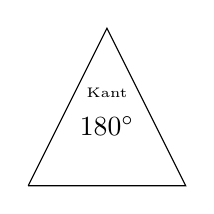
\begin{tikzpicture}
\draw (0,0) -- (1,2) -- (2,0) -- (0,0);
\draw (1,1) node[anchor=south]{\tiny Kant}node[anchor=north]{$180^\circ$};
\end{tikzpicture}
\column{.55\textwidth}
Kant: Mathematics is synthetic a priori.\\
Frege: Mathematics is analytic.
\end{columns}
}

\frame{{\href{https://www.maa.org/programs/maa-awards/writing-awards/the-three-crises-in-mathematics-logicism-intuitionism-and-formalism}{\textcolor{fore}{Philosophy of Math: Logicism/Intuitionism/Formalism}}}
\begin{figure}
	\includegraphics[width=.9\textwidth,angle=0,origin=c]{img/cartoon-foundations.pdf}
\end{figure}
\begin{table}
\begin{tabu}{c|c|c}
\hline
Logicism & Intuitionism & Formalism\\
\hline
$\frac{\mathit{Mathematics}}{\mathit{Logic}}$ & $\frac{\frac{\mathit{Logic}}{\mathit{Mathematics}}}{\mathit{Mind}}$ & $\frac{\mathit{Mathematics}}{\mathit{Game}}$\\
\hline
Realism & Conceptualism & Nominalism\\
\hline
\end{tabu}
\end{table}
}

%-------------------------------------%
\subsection{After G\"odel}
%-------------------------------------%

\frame{{Leibniz \& Hilbert --- Dream Shattered\dots}
	\centering
\begin{columns}
\column{.45\textwidth}
	\begin{figure}
		\includegraphics[width=.7\textwidth]{img/domino}
	\end{figure}
\column{.5\textwidth}
	\begin{figure}
		\includegraphics[width=\textwidth]{img/scream.jpg}
	\end{figure}
\end{columns}
}

\frame{{G\"odel 1906-1978}
\centerline{\fbox{\textcolor{blue}{``I am unprovable.''\footnote{\tiny G\"odel: On formally undecidable propositions of Principia Mathematica and related systems.}}}}
	\begin{columns}
		\column{0.6\textwidth}
			\begin{itemize}
				\item Completeness.\\
				\textcolor{blue}{\small I think (consistently), therefore I am.\\ (Consistency implies existence.)}
				\item Incompleteness.
				\begin{enumerate}
					\item \textcolor{blue}{\small provable $<$ true}
					\item \textcolor{blue}{\small un-self-aware}
				\end{enumerate}
				\item Consistency of AC and CH.
			\end{itemize}\vspace{-7pt}
			\begin{figure}
				\includegraphics[width=0.45\textwidth,angle=0,origin=c]{img/escher-book}
			\end{figure}
		\column{0.4\textwidth}
			\begin{figure}
				\includegraphics[width=\textwidth,angle=0,origin=c]{img/godel-painting}
			\end{figure}
	\end{columns}
}

\frame{{Tarski 1901-1983}
\begin{center}
``snow is white'' is true iff snow is white.
\end{center}
\begin{center}
	\fbox{\textcolor{blue}{``I am false.''}\footnote{\tiny Tarski: On the Concept of Truth in Formalized Languages.\\ Tarski: The Semantic Conception of Truth and the Foundations of Semantics.}}
\end{center}
\begin{columns}
\column{.22\textwidth}
\begin{figure}
\includegraphics[width=\textwidth,angle=0,origin=c]{img/tarski-painting}
\end{figure}
\column{.72\textwidth}
\begin{center}
\textcolor{red}{\underline{Model Theory}}
\end{center}
\begin{alertblock}{Undefinability of Truth}
Arithetical truth can't be defined in arithmetic.
\end{alertblock}
\begin{tcolorbox}
	The theory of real closed fields / elementary geometry is complete and decidable.
\end{tcolorbox}
\end{columns}
}

\frame{{Turing 1912-1954}\vspace{-1ex}
	\begin{columns}[onlytextwidth]
		\column{0.62\textwidth}
			\begin{itemize}
				\item Universal Turing Machine.
				\item Church-Turing Thesis.
				\item Halting Problem.
				\item Undecidability.
				\item Oracle Machine.
				\item Computable Absolutely Normal Number.
				\item Turing Test.
				\item Morphogenesis.
				\item Good-Turing Smoothing.
				\item Enigma.
			\end{itemize}
		\column{0.35\textwidth}
			\begin{figure}
				\includegraphics[width=\textwidth,angle=0,origin=c]{img/turing13}
			\end{figure}
	\end{columns}
	\begin{figure}\vspace*{-2.9cm}
		\begin{center}
			\[
			\begin{array}{c}
			\textcolor{darkgreen}{\boxed{\infer{\boxed{\surd}}{\boxed{\times} & \boxed{\times}}}}\\
			\qquad\textcolor{red}{\mapDown}\;\textcolor{purple}{\longrightarrow}\\
			\colorbox{cyan}{\begin{tabu}{c|c|c|c|c|c|c|c|c}
				\hline
				\;$\cdots$ & $0$ & $1$ & \textcolor{green}{$0$} & \textcolor{red}{$1$} & \textcolor{green}{$0$} & $1$ & $0$ & $\cdots$\\
				\hline
				\end{tabu}}
			\end{array}
			\]
		\end{center}
	\end{figure}\vspace{-0.6cm}
	\centerline{\fbox{\textcolor{red}{What is ``effective procedure''?\footnote{\tiny Turing: On computable numbers, with an application to the Entscheidungsproblem.}} --- \textcolor{red}{\underline{Recursion Theory}}}}
}

%%%%%%%%%%%%%%%%%%%%%%%%%%%%%%%
\section{Propositional Logic}
%%%%%%%%%%%%%%%%%%%%%%%%%%%%%%%

%%%%%%%%%%%%%%%%%%%%%%%%%%%%
\subsection{What is Logic?}
%%%%%%%%%%%%%%%%%%%%%%%%%%%%

\frame{{What is Logic?}
	\begin{itemize}
		\item Arithmetic --- the study of numbers.
		\item Geometry --- the study of figures.
		\item Algebra --- the study of mathematical symbols.
		\item Logic --- the study of logical notions.
		\item Set Theory --- the study of sets.
	\end{itemize}
	\begin{itemize}
		\item What is a number?
		\item What is a line?
		\item What is a set?
		\item What is a logical notion?
	\end{itemize}
}

\frame{{What is Mathematics?}
	\begin{quote}\it
		Mathematics is the art of giving the same name to different things.\par
		\hfill --- {\sl Henri Poincar\'e}
		
		Not substance but invariant form is the carrier of the relevant mathematical information.\par
		\hfill --- {\sl F. William Lawvere}
		
		Mathematics may be defined as the subject in which we never know what we are talking about, nor whether what we are saying is true.\par
		\hfill --- {\sl Bertrand Russell}
	\end{quote}
}

\frame{{What is Geometry? --- Klein's Erlangen Programm}
	\begin{block}{What is Geometry?}
		The study of \emph{invariants} under \emph{a group of transformations}.
	\end{block}
	\begin{columns}
		\column{0.63\textwidth}
		\boxed{\vbox{\resizebox{0.82\textwidth}{!}{\begin{minipage}{\textwidth}
						
\begin{tikzpicture}[scale=0.5]
						\draw[blue,fill=blue,nearly transparent,opacity=.5] (0,0) -- (3,0) -- (3,3) -- (0,3) -- cycle;
						\draw[blue,fill=blue,nearly transparent,opacity=.5] (5.5,0) -- (8.5,0) -- (8.5,3) -- (5.5,3) -- cycle;
						\node at (14,1.5) {\huge isometry};
						\end{tikzpicture}
						
						
\begin{tikzpicture}[scale=0.5]
						\draw[blue,fill=blue,nearly transparent,opacity=.5] (0,0) -- (3,0) -- (3,3) -- (0,3) -- cycle;
						\draw[blue,fill=blue,nearly transparent,opacity=.5] (5,-.5) -- (9,-.5) -- (9,3.5) -- (5,3.5) -- cycle;
						\node at (14,1.5) {\huge similarity};
						\end{tikzpicture}
						
						
\begin{tikzpicture}[scale=.5]
						\draw[blue,fill=blue,nearly transparent,opacity=.5] (0,0) -- (3,0) -- (3,3) -- (0,3) -- cycle;
						\draw[blue,fill=blue,nearly transparent,opacity=.5] (5,1.5) -- (7,0.5) -- (9,1.5) -- (7,2.5) -- cycle;
						\node at (14,1.5) {\huge affinity};
						\end{tikzpicture}
						
						
\begin{tikzpicture}[scale=.5]
						\draw[blue,fill=blue,nearly transparent,opacity=.5] (0,0) -- (3,0) -- (3,3) -- (0,3) -- cycle;
						\draw[blue,fill=blue,nearly transparent,opacity=.5] (5,0.5) -- (9,0.5) -- (8,2.5) -- (6,2.5) -- cycle;
						\node at (14,1.5) {\huge projection};
						\end{tikzpicture}
						
						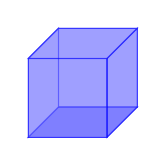
\begin{tikzpicture}[scale=.5]
						\coordinate (O) at (0,0,0);
						\coordinate (A) at (0,2,0);
						\coordinate (B) at (0,2,2);
						\coordinate (C) at (0,0,2);
						\coordinate (D) at (2,0,0);
						\coordinate (E) at (2,2,0);
						\coordinate (F) at (2,2,2);
						\coordinate (G) at (2,0,2);
						\draw[blue,fill=blue,nearly transparent,opacity=.5] (O) -- (C) -- (G) -- (D) -- cycle;% Bottom Face
						\draw[blue,fill=blue!50,nearly transparent,opacity=.5] (O) -- (A) -- (E) -- (D) -- cycle;% Back Face
						\draw[blue,fill=blue!50,nearly transparent,opacity=.5] (O) -- (A) -- (B) -- (C) -- cycle;% Left Face
						\draw[blue,fill=blue!50,nearly transparent,opacity=.5] (D) -- (E) -- (F) -- (G) -- cycle;% Right Face
						\draw[blue,fill=blue!50,nearly transparent,opacity=.5] (C) -- (B) -- (F) -- (G) -- cycle;% Front Face
						\draw[blue,fill=blue!50,nearly transparent,opacity=.5] (A) -- (B) -- (F) -- (E) -- cycle;% Top Face
						\end{tikzpicture}\qquad\quad\;
						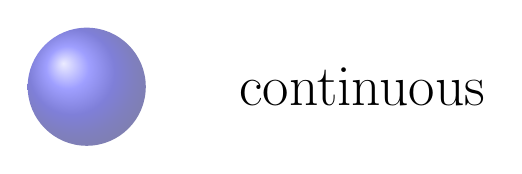
\begin{tikzpicture}
						\node[circle,shading=ball,blue!50,nearly transparent,opacity=.5,minimum width=1.5cm] (ball) at (0,0) {};
						\node at (3.5,0) {\huge continuous};
						\end{tikzpicture}
		\end{minipage}}}}
		\column{0.21\textwidth}\vspace{-4pt}
		\begin{figure}[H]
			\begin{center}
				\includegraphics[width=\textwidth,angle=0,origin=c]{img/klein}\caption{\scriptsize Felix Klein}
			\end{center}
		\end{figure}
	\end{columns}
}

\frame{{What is Geometry? --- Klein's Erlangen Programm}\vspace{-1ex}
\begin{figure}[H]
\includegraphics[width=.6\textwidth]{img/doughnut-cup.png}
\end{figure}\vspace{-4ex}
	\begin{table}
		\begin{tabu}{c|c|c|c|c|c}
			\hline
		    & isometry & similarity & affine & projective & continuous\\
			\hline
			location &  &  &  &  & \\
			\hline
			length & $\checkmark$ &  &  &  & \\
			\hline
			area & $\checkmark$ &  &  &  & \\
			\hline
			perpendicularity & $\checkmark$ & $\checkmark$ &  &  & \\
			\hline
			parallelism & $\checkmark$ & $\checkmark$ & $\checkmark$ &  & \\
			\hline
			collinearity & $\checkmark$ & $\checkmark$ & $\checkmark$ & $\checkmark$ & \\
			\hline
			concurrence & $\checkmark$ & $\checkmark$ & $\checkmark$ & $\checkmark$ & \\
			\hline
			connectedness &  $\checkmark$ & $\checkmark$ & $\checkmark$ & $\checkmark$ & $\checkmark$\\
			\hline
		\end{tabu}
	\end{table}\vspace{-1ex}
	\begin{quote}\it
	Given a manifold, and a transformation group acting on it, to study its invariants.\hfill --- {\sl Felix Klein}
	\end{quote}
}

\frame{{Klein's Erlangen Programm vs Logic}
	\centerline{\textcolor{red}{\Large What is Logic?}\footnote{\href{https://www.tandfonline.com/doi/abs/10.1080/01445348608837096}{Tarski: What are logical notions?}}}
	\begin{tcolorbox}
		Logic is the science that investigates the principles of \textcolor{red}{valid} reasoning.
	\end{tcolorbox}
	\centering\fbox{what follows from what}
	\begin{quote}\it
		The art of thinking and reasoning in strict accordance with the limitations and incapacities of the human misunderstanding.\textcolor{red}{$\sideset{^\circledcirc}{^\circledcirc}{\mathop{\hat{o}}}$}\par\hfill --- \sl The Devil's Dictionary
	\end{quote}
	\begin{tcolorbox}[colback=cyan!3,colframe=back!85]\centering
		The study of \textcolor{red}{invariants} under \textcolor{red}{all automorphisms} \textcolor{blue}{(symmetries)}.
	\end{tcolorbox}
}

\frame{{Logic $\to$ Truth}
	\begin{quote}\it
		\emph{Truth} points the way for logic, just as beauty does for aesthetics, and goodness for ethics.\par
		\hfill --- {\sl Frege}
	\end{quote}
	\centerline{\xymatrix @C=1pc{
					*+++[o][F=]{\txt{\textit{\textbf{\emph{\underline{\textcolor{blue}{{\text{Form}}}}}}}}}&&&&&&*+++[o][F=]{\txt{\textit{\textbf{\emph{\underline{\textcolor{blue}{{\text{Form}}}}}}}}}\\
					&&&&
					\ar@1{<--}^*++[F-]{\text{\footnotesize endow}} "1,7";"5,4"
					&&&\\
					\ar@1{-->}_*++[F-]{\text{\footnotesize suspend}} "1,1";"5,4"
					&&&&&\\
					\ar@1{->}^*++[F-]{\textcolor{red}{\text{\footnotesize transform}}} "1,1";"1,7"\\
					&&&*+++[F-]{\txt{\textit{\textbf{\emph{\textcolor{blue}{{\text{\small Meaning}}}}}}}}&&}}
}

\frame{{}
\begin{gather*}
\textcolor{red}{{\text{Natural Language}}}\\
\MapDown{\text{represents}}\\
\fbox{Formal Language (Syntax)}\\
\bigg{\Downarrow}\rlap{\text{\footnotesize expresses}}\\
\fbox{Theory (calculus $\vdash$)}\\
\bigg{\Downarrow}\llap{\text{\footnotesize interprets\;\;\;}}\bigg{\Uparrow}\rlap{\text{\footnotesize characterizes}}\\
\fbox{Models (semantics $\vDash$)}\\
\MapUp{\text{represents}}\\
\qquad\qquad\dots\dots\dots\dots\dots\dots\dots\dots\dots\dots\dots\dots\dots\dots \text{semantic gap}\\
\textcolor{red}{{\text{Real World}}}
\end{gather*}
}

%%%%%%%%%%%%%%%%%%%%%%%%%%%%%%%
\subsection{Syntax}
%%%%%%%%%%%%%%%%%%%%%%%%%%%%%%%

\frame{{Propositional Logic}
	\begin{itemize}
		\item Language.
		
		Building blocks of propositional logic language.
		\item Syntax.
		
		Propositional symbols and propositional formulas.
		\item Semantics.
		
		Assign ``meaning'' to propositional formulas by first assigning ``meaning'' to propositional symbols.
		\item Calculus.
		
		Axioms and inference rules.
	\end{itemize}
}

\frame{{Syntax}
		\begin{block}{Language}
			\[\mathscr{L}^0:=\{\textcolor{darkgreen}{\neg},\wedge,\vee,\textcolor{darkgreen}{\to},\leftrightarrow,(,)\}\cup\mathscr{P}\]
		\end{block}
		where $\mathscr{P}:=\{p_1,\dots,p_n,(\dots)\}$.
		\begin{block}{Well-Formed Formula $\mathrm{WFF}$}
			\[\varphi::=p_i\mid \textcolor{darkgreen}{(\neg\varphi)}\mid (\varphi\wedge\varphi)\mid (\varphi\vee\varphi)\mid \textcolor{darkgreen}{(\varphi\to\varphi)}\mid (\varphi\leftrightarrow\varphi)\]
		\end{block}
		\begin{itemize}
			\item $\bot:=(\varphi\wedge(\neg\varphi))$
			\item $\top:=(\neg\bot)$
		\end{itemize}
		\begin{example}
			\begin{itemize}
				\item Lily is (not) beautiful.
				\item If wishes are horses, then beggars will ride.
				\item Lily is beautiful and/or/iff $2$ is not a prime number.
			\end{itemize}
		\end{example}
}

\frame{{Well-Formed Formula}
	\setlength\abovedisplayskip{0pt}
	\setlength\belowdisplayskip{0pt}\vspace{-2pt}\centering
	\begin{overpic}[scale=0.45]{img/panda.png}
	\put(1,75){\textcolor{blue}{\footnotesize\textbf{A panda eats\textcolor{red}{\Large,}shoots and leaves.}}}
	\end{overpic}\vspace{-3ex}
	\begin{definition}[Formula-Building Operator]
		\begin{columns}
			\column{0.3\textwidth}
				\begin{align*}
				\mathscr{E}_\neg(\varphi)&:=(\neg\varphi)\\
				\mathscr{E}_\wedge(\varphi,\psi)&:=(\varphi\wedge\psi)\\
				\mathscr{E}_\vee(\varphi,\psi)&:=(\varphi\vee\psi)\\
				\mathscr{E}_\to(\varphi,\psi)&:=(\varphi\to\psi)\\
				\mathscr{E}_\leftrightarrow(\varphi,\psi)&:=(\varphi\leftrightarrow\psi)
				\end{align*}
			\column{0.3\textwidth}
				\boxed{\vbox{
					\begin{align*}
					\mathscr{E}_\neg(\varphi)&:=\neg\varphi\\
					\mathscr{E}_\wedge(\varphi,\psi)&:=\wedge\varphi\psi\\
					\mathscr{E}_\vee(\varphi,\psi)&:=\vee\varphi\psi\\
					\mathscr{E}_\to(\varphi,\psi)&:=\to\varphi\psi\\
					\mathscr{E}_\leftrightarrow(\varphi,\psi)&:=\leftrightarrow\varphi\psi
					\end{align*}}}
		\end{columns}
	\end{definition}
}

\frame{{Well-Formed Formula}
	\begin{definition}[Construction Sequence]
		A construction sequence $(\alpha_1,\dots,\alpha_n)$ is a finite sequence of expressions s.t. for each $i\leq n$ we have at least one of 
		\begin{align*}
		&\alpha_i=p_i\quad\text{for some $i$}\\
		&\alpha_i=\mathscr{E}_\neg(\alpha_j)\quad\text{for some $j$}\\
		&\alpha_i=\mathscr{E}_\star(\alpha_j,\alpha_k)\quad\text{for some $j<i, k<i$}\\
		&\text{where}\;\star\in\{\wedge,\vee,\to,\leftrightarrow\}.
		\end{align*}
	\end{definition}
	\begin{definition}[Well-Formed Formula]
	A formula $\varphi$ is a well-formed formula (wff) iff there is some construction sequence $(\alpha_1,\dots,\alpha_n)$ and $\alpha_n=\varphi$.
	\end{definition}
}

\frame{{Generation --- Bottom Up vs Top Down}
	\begin{tcolorbox}[colback=cyan!3,colframe=back!85,title=Problem]
		Given a class $\mathcal{F}$ of functions over $U$, how to \textcolor{blue}{generate} a certain subset of $U$ by starting with some initial elements $B\subset U$?
	\end{tcolorbox}
	\begin{columns}
		\column{0.5\textwidth}
			\setlength\abovedisplayskip{0pt}
			\begin{tcolorbox}[colback=cyan!3,colframe=back!85,title=Bottom Up]\vspace{-4pt}
				\begin{align*}
				C_0&:=B\\ C_{n+1}&:=C_n\cup\bigcup\limits_{f\in\mathcal{F}}\left\{f(\bm{x})\colon \bm{x}\in C_n\right\}\\
				C_*&:=\bigcup\limits_{n\in\mathbb{N}} C_n
				\end{align*}
				\[\mathit{deg}(\bm{x}):=\mu n\left[\bm{x}\in C_n\right]\]
			\end{tcolorbox}
		\column{0.53\textwidth}
			\begin{tcolorbox}[colback=cyan!3,colframe=back!85,title=Top Down]
				\begin{itemize}
					\item A set $S$ is \textcolor{red}{closed under a function} $f$ if for all $\bm{x}$: $\bm{x}\in S\to f(\bm{x})\in S$.
					\item A set $S$ is \textcolor{blue}{inductive} if  $B\subset S$ and for all $f\in\mathcal{F}$: $S$ is closed under $f$.
					\item $C^*:=\bigcap\{S\colon S\mbox{ is inductive}\}$
				\end{itemize}
			\end{tcolorbox}
	\end{columns}
}

\frame{{Bottom Up vs Top Down}
	\begin{tcolorbox}[colback=cyan!3,colframe=back!85,title=$10$块钱最多可以喝几瓶啤酒?$\sideset{^\circledcirc}{^\circledcirc}{\mathop{\hat{o}}}$]
		\begin{itemize}
		\item $2$块钱买$1$瓶啤酒。
		\item $2$个空瓶换$1$瓶啤酒。
		\item $4$个瓶盖换$1$瓶啤酒。
		\end{itemize}
	\end{tcolorbox}
}

\frame{{Generation --- Bottom Up vs Top Down}
	\begin{example}
		Let $B:=\{0\}, \mathcal{F}:=\{S,P\}, S(x):=x+1, P(x):=x-1$
		\[C_*=\{\dots,-2,-1,0,1,2,\dots\}\]
		There is more than one way of obtaining a member of $C_*$, e.g. $1=S(0)=S(P(S(0)))$.
	\end{example}
	\setlength\abovedisplayskip{0pt}
	\setlength\belowdisplayskip{0pt}
	\begin{theorem}[Bottom up and Top down]
		\[C_*=C^*\]
	\end{theorem}
	\begin{proof}
		($C^*\subset C_*$): to show $C_*$ is inductive.\\
		($C_*\subset C^*$): for any $( x_1,\dots,x_n)$, if $x_j\in C^*$ for all $j<i$, then $x_i\in C^*$. So by induction on $i$, it follows that, $x_i\in C^*$ for all $i\leq n$.
	\end{proof}
}

\frame{{Induction Principle for WFF}
	\begin{theorem}[归纳原理]
		令$\Psi$为一个关于合式公式的性质。假设
		\begin{itemize}
		\item $\Psi$对所有的命题符号成立;并且
		\item $\Psi$对公式构造运算封闭。
		\end{itemize}
		那么,$\Psi$对所有的合式公式都成立。
	\end{theorem}
	\begin{proof}
		\[\mathrm{WFF}_*=\mathrm{WFF}^*\subset\Psi\]
	\end{proof}
	\[\Psi(0)\wedge\forall k\in\mathbb{N}(\Psi(k)\to \Psi(k+1))\to\forall n\in\mathbb{N}\Psi(n)\]
	\[\Psi(k):=\Psi(\mathrm{WFF}_k)\]
}

\frame{{Induction vs Recursion}
\begin{figure}[H]
\includegraphics[width=.5\textwidth]{img/hanoi.pdf}
\end{figure}
\begin{center}
$\psi(n)\equiv$ ``$n$ rings needs $2^n-1$ moves.''
\end{center}
\begin{tcolorbox}
\begin{enumerate}
\item Never leave milk on any day without leaving milk
the next day as well.
\item Leave milk today.
\end{enumerate}
\end{tcolorbox}
\centering
\fbox{Leave milk today and read this note again tomorrow.}
}

\frame{{Subformula}
	\begin{definition}[Subformula]
		The set $\mathrm{Sub}(\varphi)$ of subformulas of a wff $\varphi$ is the smallest set $\Gamma$ that satisfies
		\begin{enumerate}
			\item $\varphi\in\Gamma$
			\item $\neg\psi\in\Gamma\implies\psi\in\Gamma$
			\item $\psi\to\chi\in\Gamma\implies\psi,\chi\in\Gamma$
		\end{enumerate}
	\end{definition}
	\begin{tcolorbox}
		\[
		\mathrm{Sub}(\varphi):=
		\begin{cases}
		\varphi &\text{if}\;\varphi=p\\
		\{\varphi\}\cup \mathrm{Sub}(\psi) &\text{if}\;\varphi=\neg\psi\\
		\{\varphi\}\cup \mathrm{Sub}(\psi)\cup \mathrm{Sub}(\chi) &\text{if}\;\varphi=\psi\to\chi
		\end{cases}
		\]
	\end{tcolorbox}
}

\frame{{Unique Readability, Unique Tree}\vspace{-21pt}
	\begin{figure}
		\[((\neg p)\wedge q)\to(p\wedge(q\vee(\neg r)))\]
		\begin{tikzpicture}[level distance=12mm,outer sep=1mm,inner sep=0,
		level 1/.style={sibling distance=20mm},
		level 2/.style={sibling distance=15mm},
		level 3/.style={sibling distance=15mm},
		level 4/.style={sibling distance=15mm}]
		\begin{scope}[nodes={blue,minimum size=5mm}]
		\node (e) {$\to$}
		child { node (l) {$\wedge$}
			child { node (ll) {$\neg$}
				child { node (lll) {$\textcolor{red}{p}$}
				}
			}
			child { node (lr) {\!\!\!\!$\textcolor{red}{q}$}
			}
		}
		child { node (r) {$\wedge$}
			child { node (rl) {\;\;\;$\textcolor{red}{p}$}
			}
			child { node (rr) {$\vee$}
				child { node (rrl) {$\textcolor{red}{q}$}
				}
				child { node (rrr) {$\neg$}
					child { node (rrrr) {$\textcolor{red}{r}$}
					}
				}
			}
		};
		\end{scope}
		\end{tikzpicture}
	\end{figure}
	\centering subformula vs subtree
}

\frame{{Balanced-Parentheses}
	\begin{corollary}[Balanced-Parentheses]
		In any wff, the number of left parentheses is equal to the number of right parentheses.
	\end{corollary}
	\begin{proof}
		Let $S$ be the set of ``balanced'' wffs.\\
		Base step: the propositional symbols have zero parentheses.\\
		Inductive step: obviously.
	\end{proof}
}

\frame{{Left-Weighted-Parentheses}
	\begin{lemma}
		Any proper initial segment of a wff contains an excess of left parentheses. Thus no proper initial segment of a wff can itself be a wff.
	\end{lemma}
	\setlength\abovedisplayskip{0pt}
	\setlength\belowdisplayskip{0pt}
	\begin{proof}
		Consider $\varphi=(\alpha\wedge\beta)$. The proper initial segments of $(\alpha\wedge\beta)$ are the following:
		\begin{enumerate}
			\item $($
			\item $(\alpha_0$\hfill [inductive hypothesis]
			\item $(\alpha$\hfill [balanced-parentheses]
			\item $(\alpha\wedge$\hfill [balanced-parentheses]
			\item $(\alpha\wedge\beta_0$\hfill [inductive hypothesis]
			\item $(\alpha\wedge\beta$\hfill [balanced-parentheses]
		\end{enumerate}
	\end{proof}
}

\frame{{Unique Readability}
	\begin{theorem}[Unique Readability Theorem]
		The five formula-building operations, when restricted to the set of wffs,
		\begin{enumerate}
			\item are injective, and
			\item have ranges that are disjoint from each other and from the set of proposition symbols.
		\end{enumerate}
	\end{theorem}
	\begin{proof}
		\begin{columns}
			\column{0.6\textwidth}
				To show $\mathscr{E}_\wedge$ is ono-to-one.
				\begin{align*}
				(\varphi\wedge\psi)&=(\alpha\wedge\beta)\\
				&\Downarrow\\
				\varphi\wedge\psi)&=\alpha\wedge\beta)\\
				&\Downarrow\\
				\varphi&=\alpha &[Lemma]
				\end{align*}
			\column{0.4\textwidth}
				then it follows $\psi=\beta$.\\
				
				Similarly, we can prove
				\[(\varphi\wedge\psi)\neq(\alpha\to\beta)\]
		\end{columns}
	\end{proof}
}

\frame{{Omitting Parentheses}
	\begin{enumerate}
		\item The outermost parentheses need not be explicitly mentioned.
		\item We order the boolean connectives according to decreasing binding strength: $\neg, \wedge, \vee, \to, \leftrightarrow$.
		\item Where one connective symbol is used repeatedly, grouping is to the right.
	\end{enumerate}
	\[1+2*3\]
}

%%%%%%%%%%%%%%%%%%%%%%%%%%%%%%%
\subsection{Semantics}
%%%%%%%%%%%%%%%%%%%%%%%%%%%%%%%

\frame{{Assignment}
	\begin{itemize}
		\item A truth assignment for $\mathscr{L}^0$ is a function
		\[\nu\colon\mathscr{P}\to\{0,1\}\]
		\item Such a truth assignment can be uniquely extended to $\overline{\nu}\colon\mathrm{WFF}\to\{0,1\}$ satisfying the following condition:\\\vspace{2ex}
		\centering\begin{minipage}{.75\textwidth}
		\begin{tcolorbox}[colback=cyan!3,colframe=back!85]
			\begin{enumerate}
				\item $\overline{\nu}(p)=\nu(p)$ for $p\in\mathscr{P}$
				\item $\overline{\nu}(\neg\varphi)=1-\overline{\nu}(\varphi)$
				\item $\overline{\nu}(\varphi\to\psi)=1-\overline{\nu}(\varphi)+\overline{\nu}(\varphi)\cdot\overline{\nu}(\psi)$
				\item $\overline{\nu}(\varphi\wedge\psi)=\min\{\overline{\nu}(\varphi),\overline{\nu}(\psi)\}$
				\item $\overline{\nu}(\varphi\vee\psi)=\max\{\overline{\nu}(\varphi),\overline{\nu}(\psi)\}$
				\item $\overline{\nu}(\varphi\leftrightarrow\psi)=\overline{\nu}(\varphi)\cdot\overline{\nu}(\psi)+(1-\overline{\nu}(\varphi))\cdot(1-\overline{\nu}(\psi))$
			\end{enumerate}
		\end{tcolorbox}
		\end{minipage}
	\end{itemize}
}

\frame{{Freeness vs Unique Readability}
	\begin{definition}
		The set $C$ is \textcolor{red}{freely generated} from $B$ by a class of functions $\mathcal{F}$ iff in addition to the requirements for being generated, the following conditions hold:
		\begin{enumerate}
			\item for every $f\in\mathcal{F}$: $f{\restriction_C}$ is injective.
			\item the range of $f{\restriction_C}$ for all $f\in\mathcal{F}$, and the set $B$ are pairwise disjoint.
		\end{enumerate}
	\end{definition}
}

\frame{{Recursion Theorem}
\begin{columns}
\column{.8\textwidth}
	\begin{theorem}[Recursion Theorem]
		Assume that $C$ is \textcolor{red}{freely generated} from $B$ by $\mathcal{F}$, and for every $f\in\mathcal{F}$ we have $F_f\colon V^n\to V$, where $n=\mathit{arity}(f)$. Then for every function $h\colon B\to V$, there exists a unique function $\overline{h}\colon C\to V$ s.t.
		\begin{enumerate}
			\item $\overline{h}{\restriction_B}=h$
			\item for all $f\in\mathcal{F}$ and all $x_1,\dots,x_n\in C$: \[\overline{h}(f(x_1,\dots,x_n))=F_f\big(\overline{h}(x_1),\dots,\overline{h}(x_n)\big)\]
		\end{enumerate}
	\end{theorem}
\column{.15\textwidth}
\xymatrix{B \ar[dr]_{h} \ar[r] &  C \ar[d]^{\overline{h}}\\
&  V}
\end{columns}
	\begin{itemize}
		\item $h$ tells you how to color the initial elements in $B$;
		\item $F_f$ tells you how to convert the color of $\bm{x}$ into the color of $f(\bm{x})$.
	\end{itemize}
	\textcolor{red}{Danger! $F_f$ is saying ``green'' but $F_g$ is saying ``red'' for the same point.}
}

\frame{{Truth Table}
			\[
			\begin{tabu}{c|c}
			\hline
			\textcolor{red}{p} & \textcolor{darkgreen}{\neg p}\\
			\hline
			0 & 1\\
			1 & 0\\
			\hline
			\end{tabu}\qquad
			\begin{tabu}{cc|c|c|c|c}
				\hline
				\textcolor{red}{p} & \textcolor{red}{q} & \textcolor{darkgreen}{p\to q} & p\wedge q & p\vee q & p\leftrightarrow q\\
				\hline
				0 & 0 & 1 & 0 & 0 & 1\\
				0 & 1 & 1 & 0 & 1 & 0\\
				1 & 0 & 0 & 0 & 1 & 0\\
				1 & 1 & 1 & 1 & 1 & 1\\
				\hline
			\end{tabu}
			\]
		\begin{example}
			\begin{itemize}
				\item If $0=1$, then Russell is God.\\
				\item Snow is white iff $1+1=2$.
			\end{itemize}
		\end{example}
}

\frame{{Material Implication vs Cognition}
	\begin{tcolorbox}
		翻哪几张卡才能验证“如果一面是偶数,另一面肯定是红色”?
	\end{tcolorbox}
	\includegraphics[width=\textwidth]{img/wason.png}
	\begin{tcolorbox}
		未满$18$岁禁止饮酒!
	\end{tcolorbox}
}

\frame{{Tautology}
		If lily is beautiful, then the fact that $2$ is a prime number implies lily is beautiful.
		\begin{table}
			\begin{tabu}{cc|c|c}
				\hline
				\textcolor{red}{p} & \textcolor{red}{q} & $q\to p$ & $p\to q\to p$\\
				\hline
				0 & 0 & 1 & 1\\
				0 & 1 & 0 & 1\\
				1 & 0 & 1 & 1\\
				1 & 1 & 1 & 1\\
				\hline
			\end{tabu}
		\end{table}
		\begin{center}
			$2^n$ truth assignments for a set of
			$n$ propositional symbols.
		\end{center}
		\begin{itemize}
			\item $\nu\vDash\varphi$ if $\overline{\nu}(\varphi)=1$.
			\item \textcolor{red}{Logical Consequence.} \textcolor{blue}{$\Gamma\vDash\varphi$} if for any truth assignment $\nu$ s.t. $(\text{for all}\;\psi\in\Gamma\colon \nu\vDash\psi)\implies\nu\vDash\varphi$.
			\item \textcolor{red}{Tautology.} \textcolor{blue}{$\vDash\varphi$ if $\emptyset\vDash\varphi$}.
		\end{itemize}
}

\frame{
	\begin{table}
		\begin{tabu}{ccc|c}
			\hline
			\textcolor{red}{p} & \textcolor{red}{q} & \textcolor{red}{r} & $(p\to q\to r)\to (p\to q)\to p\to r$\\
			\hline
			0 & 0 & 0 & 1\\
			0 & 0 & 1 & 1\\
			0 & 1 & 0 & 1\\
			0 & 1 & 1 & 1\\
			1 & 0 & 0 & 1\\
			1 & 0 & 1 & 1\\
			1 & 1 & 0 & 1\\
			1 & 1 & 1 & 1\\
			\hline
		\end{tabu}
	\end{table}
	
	\begin{block}{What is Propositional Logic?}
		The study of invariants under all permutations in truth space $\{0,1\}^*$.
	\end{block}
}

\frame{{Truth Table --- Simplification for Tautology}
	\begin{table}\huge
		\centering
		\tabcolsep=0pt
		\begin{tabu}{*{24}c}
			&(&p&$\to$&&q&$\to$ &r&&)&$\to$ &&(&p&$\to$ &q&)&$\to$&&p&$\to$ &r&&\\
			&&&&&&&&&&$\underline{\bm{0}}$&&&&&&&&&&&&&\\
			&&&1&&&&&&&$\bm{0}$&&&&&&&$\underline{\bm{0}}$&&&&&&\\
			&&&1&&&&&&&$\bm{0}$&&&&1&&&$\bm{0}$&&&$\underline{\bm{0}}$&&&\\
			&&\textcolor{red}{1}&1&&&&\textcolor{red}{0}&&&$\bm{0}$&&&\textcolor{red}{1}&$\underline{\bm{1}}$&&&$\bm{0}$&&\textcolor{red}{1}&$\bm{0}$&\textcolor{red}{0}&&\\
			&&\textcolor{red}{1}&$\underline{\bm{1}}$&&\textcolor{red}{1}&&\textcolor{red}{0}&&&$\bm{0}$&&&\textcolor{red}{1}&$\bm{1}$&\textcolor{red}{1}&&$\bm{0}$&&\textcolor{red}{1}&$\bm{0}$&\textcolor{red}{0}&&\\
			&&\textcolor{red}{1}&$\bm{1}$&&\textcolor{red}{1}&$\underline{\bm{1}}$&\textcolor{red}{0}&&&$\bm{0}$&&&\textcolor{red}{1}&$\bm{1}$&\textcolor{red}{1}&&$\bm{0}$&&\textcolor{red}{1}&$\bm{0}$&\textcolor{red}{0}&&\\
			&&&&&&$\textcolor{red}{\times}$&&&&&&&&&&&&&&&&&
		\end{tabu}
	\end{table}
}

{\setbeamercolor{normal text}{fg=fore,bg=back}\usebeamercolor[fg]{normal text}
	\frame{{Exercises --- Translation}
		\begin{enumerate}
			\item The answer is $3$ or $6$.
			\item I am not good at logic.
			\item If you can't say it clearly, you don't understand it yourself.
			\item You understand something only if you can formalize it.
			\item I will go out unless it rains.
			\item You can pay by credit card or cheque.
			\item Neither Sarah nor Peter was to blame for the mistake.
			\item I want to buy either a new desktop computer or a laptop, but I have neither the cash nor the credit I need.
			\item If I get in the lift then it breaks, \textcolor{orange}{or} if you get in then the lift breaks.(\textcolor{orange}{???})\hfill \textcolor{cyan}{(Natural language is ambiguous!)}
			\item If we both get in the lift, then the lift breaks.
			\item $p\vee q\to r\logeq(p\to r)\wedge(q\to r)$
			\item $p\wedge q\to r\logeq(p\to r)\vee(q\to r)$
		\end{enumerate}
	}
}

\frame{{Example}
	\begin{tcolorbox}[colback=cyan!3,colframe=back!85,title=$\sideset{^\circledcirc}{^\circledcirc}{\mathop{\hat{o}}}$]
		\begin{enumerate}
			\item The programmer's wife tells him: ``Run to the store and pick up a loaf of bread. If they have eggs, get a dozen.''
			\item The programmer comes home with $12$ loaves of bread.
			\item ``Why did you buy $12$ loaves of bread!?'', his wife screamed.
			\item ``Because they had eggs!''
		\end{enumerate}	
	\end{tcolorbox}
	\begin{itemize}
		\item wife.
		\[q\wedge(p\to r)\]
		\item programmer.
		\[(\neg p\to q)\wedge(p\to s)\]
	\end{itemize}
}

{\setbeamercolor{normal text}{fg=fore,bg=back}\usebeamercolor[fg]{normal text}
	\frame{{Exercises --- Validity}
		\begin{columns}
			\column{0.5\textwidth}
				\begin{enumerate}
					\item \textcolor{green}{$p\vee q\logeq\neg p\to q\logeq(p\to q)\to q$}
					\item \textcolor{green}{$p\wedge q\logeq\neg(p\to\neg q)$}
					\item \textcolor{green}{$p\leftrightarrow q\logeq(p\to q)\wedge(q\to p)$}
					\item $p\wedge q\logeq\neg(\neg p\vee\neg q)$
					\item $p\to(q\to r)\logeq(p\wedge q)\to r$
					\item $p\to q\logeq\neg q\to\neg p$
					\item $p\wedge(q\vee r)\logeq(p\wedge q)\vee(p\wedge r)$
					\item $p\vee(q\wedge r)\logeq(p\vee q)\wedge(p\vee r)$
					\item $\neg(p\vee q)\logeq\neg p\wedge\neg q$
					\item $\neg(p\wedge q)\logeq\neg p\vee\neg q$
					\item $p\logeq p\vee(p\wedge q)$
					\item $p\logeq p\wedge(p\vee q)$
				\end{enumerate}
			\column{0.5\textwidth}
				\begin{enumerate}
					\item \textcolor{orange}{$\vDash\neg\neg p\to p$}
					\item $\vDash p\to\neg\neg p$
					\item \textcolor{orange}{$\vDash p\vee\neg p$}
					\item $\vDash \neg(p\wedge\neg p)$
					\item $\vDash p\wedge\neg p\to q$
					\item \textcolor{orange}{$\vDash (p\to q)\wedge(\neg p\to q)\to q$}
					\item $\vDash (p\to q)\wedge(p\to\neg q)\to\neg p$
					\item \textcolor{orange}{$\vDash (\neg p\to q)\wedge(\neg p\to\neg q)\to p$}
					\item \textcolor{orange}{$\vDash((p\to q)\to p)\to p$}
				\end{enumerate}
				\begin{enumerate}
					\item $\Gamma,\varphi\vDash\psi\iff\Gamma\vDash\varphi\to\psi$
					\item $\varphi\logeq\psi\iff\vDash\varphi\leftrightarrow\psi$
					\item $\varphi\vee\psi, \neg\varphi\vee\chi\vDash\psi\vee\chi$
				\end{enumerate}
		\end{columns}
	}
}

\frame{{}
	\begin{columns}
		\column{0.3\textwidth}
			\begin{prooftree}
				\AxiomC{$p\to q$}
				\noLine
				\UnaryInfC{$\phantom{p\to} q$}
				\alwaysSingleLine
				\UnaryInfC{$p$}
			\end{prooftree}
		\column{0.3\textwidth}
			\begin{prooftree}
				\AxiomC{$p\to q$}
				\noLine
				\UnaryInfC{$\neg p\phantom{\to q}$}
				\alwaysSingleLine
				\UnaryInfC{$\neg q$}
			\end{prooftree}
		\column{0.3\textwidth}
			\begin{prooftree}
				\AxiomC{$p\vee q$}
				\noLine
				\UnaryInfC{$p$}
				\alwaysSingleLine
				\UnaryInfC{$\neg q$}
			\end{prooftree}
	\end{columns}
	\begin{prooftree}
		\AxiomC{I think, therefore I am}
		\noLine
		\UnaryInfC{I do not think\phantom{foreI am}}
		\alwaysSingleLine
		\UnaryInfC{Therefore I am not}
	\end{prooftree}
	\begin{prooftree}
		\AxiomC{美女是老王或大黄杀的}
		\noLine
		\UnaryInfC{老王是凶手}
		\alwaysSingleLine
		\UnaryInfC{大黄是无辜的}
	\end{prooftree}
\begin{tcolorbox}
\begin{quote}\it
	\textcolor{blue}{By all means marry; if you get a good wife, you'll be happy. If you get a bad one, you'll become a philosopher.} \par\hfill --- {\sl \textcolor{red}{Socrates}}
\end{quote}
\end{tcolorbox}
}

\frame{{Example}
\begin{tcolorbox}
好货不贱,贱货不好。
\end{tcolorbox}
\begin{tcolorbox}
如果把整个太平洋的水倒出,也浇不灭我对你爱情的火焰。
整个太平洋的水倒得出吗?不行。
所以,我不爱你。
\end{tcolorbox}
\begin{tcolorbox}
如果把整个浴缸的水倒出,也浇不灭我对你爱情的火焰。
整个浴缸的水倒得出吗?可以。
所以,是的,我爱你。
\end{tcolorbox}
}

\frame{{Example}
	\begin{tcolorbox}
	\begin{itemize}
		\item 如果你工作,就能挣钱;如果你赋闲在家,就能悠然自在。你要么工作要么赋闲,总之,你能挣钱或者能悠然自在。
		\item 如果你工作,就不能悠然自在;如果你赋闲在家,就不能挣钱。你要么工作要么赋闲,总之,你不能悠然自在或者不能挣钱。
	\end{itemize}
	\end{tcolorbox}
	\[p\to r, q\to s\vDash p\vee q\to r\vee s\]
	\[p\to\neg s, q\to\neg r\vDash p\vee q\to\neg s\vee\neg r\]
\begin{itemize}
	\item 老婆婆有俩儿子,老大卖阳伞,老二卖雨伞,晴天雨伞不好卖,雨天阳伞不好卖……
	\item 被困失火的高楼,走楼梯会被烧死,跳窗会摔死……
\end{itemize}
}

\frame{{Example}
	\begin{tcolorbox}[title=诉讼悖论]\small
		\begin{itemize}
			\item 曾有师生签订合同:上学期间不收费,学生毕业打赢第一场官司后交学费。
			\item 可学生毕业后并未从事律师职业,于是老师威胁起诉学生。
			\item 老师说:如果我赢了,根据法庭判决,你必须交学费;如果你赢了,根据合同,你也必须交学费。要么我赢要么你赢,你都必须交学费。
			\item 学生说:如果我赢了,根据法庭判决,我不用交学费;如果你赢了,根据合同,我不用交学费。要么我赢要么你赢,我都不用交学费。
		\end{itemize}
	\end{tcolorbox}
\begin{columns}
\column{.64\textwidth}
	\[w\to p, \neg w\to p, w\vee\neg w\vDash p\]
	\[w\wedge j\to p, \neg w\wedge c\to p, w\vee\neg w\stackrel{?}{\vDash} p\]
	\[\neg w\wedge j\to\neg p, w\wedge c\to\neg p, w\vee\neg w\stackrel{?}{\vDash}\neg p\]
	\[w\wedge j\to p, \neg w\wedge c\to p, (w\wedge j)\vee(\neg w\wedge c)\vDash p\]
\column{.33\textwidth}
\includegraphics[width=\textwidth]{img/wangwang.jpg}
\end{columns}
}

\frame{{The Crocodile Dilemma}
	\begin{alertblock}{The Crocodile Dilemma}
		I will return your child iff you can correctly predict what I will do next.
	\end{alertblock}
	\[x=?\implies \vDash(x\leftrightarrow r)\to r\]
	\[
		\begin{tabu}{c|c}
		\hline
		r & (\neg r\leftrightarrow r)\to r\\
		\hline
		0 & 1\\
		1 & 1\\
		\hline
		\end{tabu}
	\]
	\[((r\vee\neg r)\leftrightarrow r)\to r\]
}

\frame{{怎么得大奖?}
	\begin{problem}[怎么得大奖?]
		\begin{itemize}
			\item 说真话得一个大奖或一个小奖。
			\item 说假话不得奖。
		\end{itemize}
	\end{problem}
\begin{itemize}
\item b: 我会得大奖。
\item s: 我会得小奖。
\end{itemize}\pause
\[x=?\implies \vDash(x\leftrightarrow b\vee s)\to b\]
\[\!\!\hspace*{-6pt}
		\begin{tabu}{cc|c|c|c}
			\hline
			b & s & (\textcolor{red}{\neg b\wedge\neg s}\leftrightarrow b\vee s)\to b & (\textcolor{red}{\neg s}\leftrightarrow b\vee s)\to b & ((\textcolor{red}{s\to b})\leftrightarrow b\vee s)\to b\\
			\hline
				0 & 0 & 1 & 1 &1\\
				0 & 1 & 1 & 1 &1\\
				1 & 0 & 1 & 1 &1\\
				1 & 1 & 1 & 1 &1\\
			\hline
		\end{tabu}
\]
}

\frame{{Gateway to Heaven}
	\begin{problem}[天堂之路]
		\begin{itemize}
			\item 你面前有左右两人守卫左右两门。
			\item 一人只说真话,一人只说假话。
			\item 一门通天堂,一门通地狱。
			\item 你只有向其中一人提问一个“是/否”问题的机会。
			\item 怎么问出去天堂的路?
		\end{itemize}
	\end{problem}
\[x=?\implies \vDash(p\to(x\leftrightarrow q))\wedge(\neg p\to(x\leftrightarrow\neg q))\]\vspace*{-2ex}
\begin{columns}
\column{.3\textwidth}
\begin{itemize}
\item p: 你说真话。
\item q: 左门通天堂。
\end{itemize}
\column{.6\textwidth}
	\begin{table}
		\begin{tabu}{cc|c|c}
			\hline
			p & q & $(p\wedge q)\vee(\neg p\wedge\neg q)$ & report\\
			\hline
				0 & \textcolor{blue}{0} & 1 & \textcolor{blue}{0}\\
				0 & \textcolor{red}{1} & 0 & \textcolor{red}{1}\\
				1 & \textcolor{blue}{0} & 0 & \textcolor{blue}{0}\\
				1 & \textcolor{red}{1} & 1 & \textcolor{red}{1}\\
			\hline
		\end{tabu}
	\end{table}
\end{columns}
}

\frame{{Proof by Contradiction}
\[(\neg p\to q)\wedge(\neg p\to\neg q)\to p\]
\begin{theorem}[Euclid's Theorem]
There are infinitely many prime numbers.
\end{theorem}
\begin{proof}
Assume to the contrary that $\mathbb{P}:=\{p_1,p_2,\dots,p_k\}$ is finite. Let $N:=\prod\limits_{i=1}^kp_i$.
$\exists p\in\mathbb{P}\colon p\mid(N+1)\;\;\&\;\;p\mid N\implies p\mid 1$.
\end{proof}
}

\frame{{Semantic Equivalence}
	\begin{itemize}
		\item Semantic equivalence is an equivalence relation between formulas.
		\item Semantic equivalence is compatible with operators.
		\[\varphi\logeq\varphi'\implies\neg\varphi\logeq\neg\varphi'\]
		\[\left.
		\begin{aligned}
		\varphi&\logeq\varphi'\\
		\psi&\logeq\psi'
		\end{aligned}\right\}\implies\varphi\star\psi \logeq \varphi'\star\psi'\]
		where $\star\in\{\wedge,\vee,\to,\leftrightarrow\}$.
		\item \textcolor{blue}{\small Equivalence relation $+$ Compatible with Operators $=$ Congruence relation}
	\end{itemize}
}

\frame{{Substitution}\vspace{-3ex}
	\begin{align*}
	p[\alpha_1/p_1,\dots,\alpha_n/p_n]&:=
	\begin{cases}
	\alpha_i &\text{if}\;p=p_i\;\text{for some}\;1\leq i\leq n\\
	p &\text{otherwise}
	\end{cases}\\
	(\neg\varphi)[\alpha_1/p_1,\dots,\alpha_n/p_n]&:=\neg\varphi[\alpha_1/p_1,\dots,\alpha_n/p_n]\\
	(\varphi\to\psi)[\alpha_1/p_1,\dots,\alpha_n/p_n]&:=\varphi[\alpha_1/p_1,\dots,\alpha_n/p_n]\to\psi[\alpha_1/p_1,\dots,\alpha_n/p_n]
	\end{align*}
	\begin{theorem}
		Consider a wff $\varphi$ and a sequence $\alpha_1,\dots,\alpha_n$ of wffs.
		\begin{enumerate}
			\item Let $\nu$ be a truth assignment for the set of all propositional symbols. Define $\rho$ to be the truth assignment for which $\rho(p_i)=\overline{\nu}(\alpha_i)$. Then $\overline{\rho}(\varphi)=\overline{\nu}\left(\varphi[\alpha_1/p_1,\dots,\alpha_n/p_n]\right)$.
			\item $\vDash\varphi\implies\vDash\varphi[\alpha_1/p_1,\dots,\alpha_n/p_n]$
		\end{enumerate}
	\end{theorem}
	\begin{example}
		\[\vDash p\vee\neg p\implies\vDash(p\wedge\neg p)\vee\neg(p\wedge\neg p)\]
	\end{example}
}

\frame{{Duality}
	\begin{theorem}
		Let $\varphi$ be a wff whose only connectives are $\neg,\wedge,\vee$. Let $\varphi^*$ be the result of interchanging $\wedge$ and $\vee$ and replacing each propositional symbol by its negation. Then $\neg\varphi\logeq\varphi^*$.
	\end{theorem}
	\begin{proof}
		Prove by induction.
		\begin{itemize}
			\item $\varphi=p_i$
			\item $\varphi=\neg\alpha$
			\item $\varphi=\alpha\wedge\beta$
			\item $\varphi=\alpha\vee\beta$
		\end{itemize}
	\end{proof}
}

%%%%%%%%%%%%%%%%%%%%%%%%%%%%%%%
\subsection{Connectives}
%%%%%%%%%%%%%%%%%%%%%%%%%%%%%%%

\frame{{Connectives}
	\begin{tcolorbox}[colback=cyan!3,colframe=back!85]
		Would we gain anything by adding more connectives to the language?
	\end{tcolorbox}
	\begin{example}[Exclusive Disjunction]
		\begin{columns}
			\column{0.7\textwidth}
				\begin{align*}
				\nu(p\dot{\vee} q)&=|\nu(p)-\nu(q)|\\
				&\Downarrow\\
				p\dot{\vee} q&\logeq(p\wedge\neg q)\vee(\neg p\wedge q)\\
				&\logeq(p\vee q)\wedge\neg(p\wedge q)\\
				&\logeq\neg(p\leftrightarrow q)
				\end{align*}
			\column{0.3\textwidth}
				\begin{table}
					\begin{tabu}{cc|c}
						\hline
						\textcolor{red}{p} & \textcolor{red}{q} & $p\dot{\vee}q$\\
						\hline
						0 & 0  & 0\\
						0 & 1  & 1\\
						1 & 0  & 1\\
						1 & 1  & 0\\
						\hline
					\end{tabu}
				\end{table}
		\end{columns}
	\end{example}
	\begin{columns}
		\column{0.2\textwidth}
			\begin{prooftree}
				\AxiomC{$p\dot{\vee} q$}
				\noLine
				\UnaryInfC{$p$}
				\alwaysSingleLine
				\UnaryInfC{$\neg q$}
			\end{prooftree}
		\column{0.2\textwidth}
			\begin{prooftree}
				\AxiomC{$p\dot{\vee} q$}
				\noLine
				\UnaryInfC{$\neg p$}
				\alwaysSingleLine
				\UnaryInfC{$q$}
			\end{prooftree}
		\column{0.2\textwidth}
			\begin{prooftree}
				\AxiomC{$p$}
				\alwaysSingleLine
				\RightLabel{\textcolor{red}{?}}
				\UnaryInfC{$p\dot{\vee} q$}
			\end{prooftree}
	\end{columns}
}

\frame{{Example}
	\setlength\abovedisplayskip{0pt}
	\setlength\belowdisplayskip{0pt}
	\begin{example}
		Let $\#$ be a three-place proposition connective.\\
		The interpretation of $\#$ is given by
		\[\nu(\#(p,q,r))=\left\lfloor\dfrac{\nu(p)+\nu(q)+\nu(r)}{2}\right\rfloor\]
		then
		\[\#(p,q,r)\logeq(p\wedge q)\vee(p\wedge r)\vee(q\wedge r)\]
	\end{example}
}

\frame{{Boolean Function}
	A $n$-place Boolean function is a function $B\colon\{0,1\}^n\to\{0,1\}$.
\[
\begin{tabu}{c|c}
					\hline
					\textcolor{red}{p} & \textcolor{darkgreen}{\neg p}\\
					\hline
					0 & 1\\
					1 & 0\\
					\hline
\end{tabu}\qquad
\begin{tabu}{cc|c|c|c|c|c}
					\hline
					\textcolor{red}{p} & \textcolor{red}{q} & \textcolor{darkgreen}{p\to q} & p\wedge q & p\vee q & p\leftrightarrow q & \cdots\\
					\hline
					0 & 0  & 1 & 0 & 0 & 1 & \cdots\\
					0 & 1  & 1 & 0 & 1 & 0 & \cdots\\
					1 & 0  & 0 & 0 & 1 & 0 & \cdots\\
					1 & 1  & 1 & 1 & 1 & 1 & \cdots\\
					\hline
\end{tabu}
\]
	\textcolor{red}{There are $2^{2^n}$ distinct Boolean functions with $n$ places.}
	\begin{definition}
		Suppose $\varphi$ is a wff whose propositional symbols are $p_1,\dots,p_n$. A Boolean function $B$ \textcolor{blue}{realized} by $\varphi$ is
		\[B_\varphi(\nu(p_1),\dots,\nu(p_n))=\overline{\nu}(\varphi)\]
	\end{definition}
}

\frame{
	\begin{theorem}[Post1921]
		Every Boolean function can be realized by some wff whose only connectives are $\neg,\wedge,\vee$.
	\end{theorem}
	\begin{proof}
		\[p_i^{x_i}:=
		\begin{cases}
		p_i &\text{if}\; x_i=1\\
		\neg p_i &\text{otherwise}
		\end{cases}\]
		\begin{columns}
			\column{0.5\textwidth}
				Case1: $B(\bm{x})=0$ for all $\bm{x}\in\{0,1\}^n$.\\
				Let $\varphi=p\wedge\neg p$.\\
				Case2: 
				\[\varphi=\bigvee\limits_{\bm{x}:B(\bm{x})=1}\bigwedge\limits_{i=1}^n p_i^{x_i}\]
			\column{0.5\textwidth}
				Case1: $B(\bm{x})=1$ for all $\bm{x}\in\{0,1\}^n$.\\
				Let $\psi=p\vee\neg p$.\\
				Case2: 
				\[\psi=\bigwedge\limits_{\bm{x}:B(\bm{x})=0}\bigvee\limits_{i=1}^n p_i^{1-x_i}\]
		\end{columns}
	\end{proof}
}

\frame{{Normal Form}
	\begin{corollary}
		Every wff which is not a contradiction is logically equivalent to a formula of \textcolor{blue}{disjunctive normal form (DNF)}: \[\bigvee\limits_{i=1}^m\bigwedge\limits_{j=1}^n\pm p_{ij}\]
	\end{corollary}
	\begin{corollary}
		Every wff which is not a tautology is logically equivalent to a formula of \textcolor{blue}{conjunctive normal form (CNF)}: \[\bigwedge\limits_{i=1}^m\bigvee\limits_{j=1}^n\pm p_{ij}\]
	\end{corollary}
}

\frame{{CNF Transformation}
	\begin{align*}
	\varphi\leftrightarrow \psi&\implies(\neg \varphi\vee \psi)\wedge(\neg \psi\vee \varphi)\\
	\varphi\to \psi&\implies \neg \varphi\vee \psi\\
	\neg(\varphi\wedge \psi)&\implies\neg \varphi\vee\neg \psi\\
	\neg(\varphi\vee \psi)&\implies\neg \varphi\wedge\neg \psi\\
	\neg\neg \varphi&\implies \varphi\\
	(\varphi_1\wedge\dots\wedge \varphi_n)\vee \psi&\implies(\varphi_1\vee \psi)\wedge\dots\wedge(\varphi_n\vee \psi)
	\end{align*}
}

\frame{{Adequate Sets of Connectives}
	\begin{definition}
		An adequate set of connectives is a set s.t. every truth function can be represented by a wff containing only connectives from that set.
	\end{definition}
	\begin{columns}
		\column{0.6\textwidth}
			\begin{itemize}
				\item $\{\neg,\wedge,\vee\}$
				\item $\{\neg,\wedge\}; \{\neg,\vee\}; \{\neg,\to\}; \{\bot,\to\}$
				\item $\{\uparrow\}; \{\downarrow\}$
				\item $\{\wedge,\vee,\to,\leftrightarrow\}; \{\neg,\leftrightarrow\}$ not adequate.
			\end{itemize}
		\begin{align*}
			\bot&:=p\wedge\neg p\\
			p\uparrow q&:=\neg(p\wedge q)\\
			p\downarrow q&:=\neg(p\vee q)\\
			\neg p&:=p\uparrow p\\
			p\wedge q&:=(p\uparrow q)\uparrow(p\uparrow q)\\
			p\vee q&:=(p\uparrow p)\uparrow(q\uparrow q)
		\end{align*}
		\column{0.4\textwidth}
			\begin{table}
				\begin{tabu}{c|c}
					\hline
					\textcolor{red}{p} & \textcolor{darkgreen}{$\bot$}\\
					\hline
					0 & 0\\
					1 & 0\\
					\hline
				\end{tabu}
			\end{table}
			\begin{table}
				\begin{tabu}{cc|c|c}
					\hline
					\textcolor{red}{p} & \textcolor{red}{q} & $p\uparrow q$ & $p\downarrow q$\\
					\hline
					0 & 0  & 1 & 1\\
					0 & 1  & 1 & 0\\
					1 & 0  & 1 & 0\\
					1 & 1  & 0 & 0\\
					\hline
				\end{tabu}
			\end{table}
	\end{columns}
}

%%%%%%%%%%%%%%%%%%%%%%%%%%%%%%%
\subsection{Formal System}
%%%%%%%%%%%%%%%%%%%%%%%%%%%%%%%

\begin{frame}[fragile]{Why Study Formal System?}
	Why truth tables are not sufficient?
	\begin{itemize}
		\item Exponential size
		\begin{itemize}
			\item \textcolor{blue}{How many \switchocg{ocg6}{times} would you have to fold a piece of paper($0.1mm$) onto itself to reach the Moon?}
			\item \href{http://nautil.us/blog/we-are-all-princes-paupers-and-part-of-the-human-family}{\textcolor{purple}{Common Ancestors of All Humans}}\\
			\textcolor{blue}{$(1)$ Someone alive $1000BC$ is an ancestor of everyone alive today;\\
				$(2)$ Everyone alive $2000BC$ is either an ancestor of nobody alive today or of everyone alive today;\\
				$(3)$ Most of the people you are descended from are no more genetically related to you than strangers are.\\
				$(4)$ Even if everyone alive today had exactly the same set of ancestors from $2000BC$, the distribution of one's ancestors from that population could be very different.}
		\end{itemize}
		\item Inapplicability beyond Boolean connectives.
	\end{itemize}
\begin{columns}
\column{.12\textwidth}
	\begin{figure}[H]
	\includegraphics[width=\textwidth]{img/grid.pdf}
	\end{figure}
\column{.1\textwidth}
\begin{ocg}{fold-paper}{ocg6}{0}
\begin{verbatim}
42
\end{verbatim}
\end{ocg}
\end{columns}
\end{frame}

\frame{{Formal System $=$ Axiom $+$ Inference Rule}
		\begin{alertblock}{Axiom Schema}
			\begin{enumerate}
				\item $\varphi\to\psi\to\varphi$
				\item $(\varphi\to\psi\to\chi)\to(\varphi\to\psi)\to\varphi\to\chi$
				\item $(\neg\varphi\to\neg\psi)\to(\neg\varphi\to\psi)\to\varphi$
			\end{enumerate}
		\end{alertblock}
		\begin{alertblock}{Inference Rule}
			\begin{prooftree}
				\AxiomC{$\varphi$\quad$\varphi\to\psi$}
				\alwaysSingleLine
				\RightLabel{\textcolor{blue}{[MP]}}
				\UnaryInfC{$\psi$}
			\end{prooftree}
		\end{alertblock}
}

\frame{{Deduction / Proof}
	\begin{center}
	\fbox{这个句子永远不能被证明}
	\end{center}
		\begin{tcolorbox}[colback=cyan!3,colframe=back!85]
			\centering\textcolor{red}{什么是“证明”?}
		\end{tcolorbox}
		\begin{definition}[Deduction]
			A deduction from $\Gamma$ is a sequence of wff $(\varphi_1,\dots,\varphi_n)$ s.t. for $k\leq n$, either
			\begin{enumerate}
				\item $\varphi_k$ is an axiom, or\\
				\item $\varphi_k\in\Gamma$, or\\
				\item for some $i<k$ and $j<k$, $\varphi_i=\varphi_j\to\varphi_k$.
			\end{enumerate}
		\end{definition}
		\begin{itemize}
			\item \textcolor{blue}{$\Gamma\vdash\varphi$} if $\varphi$ is the last member of some deduction from $\Gamma$.
			\item \textcolor{blue}{$\vdash\varphi:=\emptyset\vdash\varphi$}
		\end{itemize}
房子着火了,数学家的妻子拿起灭火器把火灭了;\\
煤气泄漏了,数学家把房子点了。
}

\frame{{Example}
	\begin{theorem}
		\[\vdash p\to p\]
	\end{theorem}
	\begin{proof}
		\begin{enumerate}
			\item $p\to(p\to p)\to p$ \hfill A1
			\item $(p\to(p\to p)\to p)\to(p\to p\to p)\to p\to p$\hfill A2
			\item $(p\to p\to p)\to p\to p$\hfill 1,2 MP
			\item $p\to p\to p$\hfill A1
			\item $p\to p$\hfill 3,4 MP
		\end{enumerate}
	\end{proof}
}

\frame{{Example}
	\begin{theorem}
		\[\vdash(\neg p\to p)\to p\]
	\end{theorem}
	\begin{proof}
		\begin{enumerate}
			\item $(\neg p \to\neg p) \to(\neg p \to p) \to p$ \hfill A3
			\item $\neg p \to \neg p$
			\item $(\neg p \to p) \to p$ \hfill 1,2 MP
		\end{enumerate}
	\end{proof}
}

\frame{{Example}
	\begin{theorem}
		\[p\to q, q \to r\vdash p \to r\]
	\end{theorem}
	\begin{proof} 
		\begin{enumerate}
			\item $(q\to r)\to (p\to q\to r)$ \hfill A1
			\item $q \to r$ \hfill Premise
			\item $p \to q \to r$ \hfill 1,2 MP
			\item $(p \to q \to r) \to (p \to q) \to p \to r$ \hfill A2
			\item $(p \to q) \to p \to r$ \hfill 4,3 MP
			\item $p \to q$ \hfill Premise
			\item $p \to r$ \hfill 5,6 MP
		\end{enumerate}
	\end{proof}
}

\frame{{Example --- Curry's Paradox\textcolor{red}{$\sideset{^\circledcirc}{^\circledcirc}{\mathop{\hat{o}}}$}}
\centering
\fbox{\textcolor{red}{如果这句话是真的那么上帝存在。}}
	\begin{block}{If this sentence is true, then I am God.}
		\[p\leftrightarrow(p\to q)\vdash q\]
	\end{block}
\begin{columns}
\column{.36\textwidth}
	\begin{proof}
		\begin{enumerate}
			\item $p\leftrightarrow(p\to q)$
			\item $p\to p\to q$
			\item $(p\to p)\to p\to q$
			\item $p\to q$
			\item $p$
			\item $q$
		\end{enumerate}
	\end{proof}
\column{.57\textwidth}
\begin{enumerate}
	\item 甲:如果我没说错,那么上帝存在。
	\item 乙:\textbf{如果你没说错,}那么上帝存在。
	\item 甲:你承认我没说错了?
	\item 乙:当然。
	\item 甲:可见我没说错。你已经承认:\textbf{如果我没说错,那么上帝存在。}所以,上帝存在。
\end{enumerate}
\end{columns}\centering
\fbox{\textcolor{red}{这句话是假的并且上帝不存在。}}
}

\frame{{Curry's Paradox --- Kiss-Kiss $\sideset{^\heartsuit}{^\heartsuit}{\mathop{\circledcirc}}$}
	\begin{tcolorbox}[colback=cyan!3,colframe=back!85,title=Smullyan实力撩妹$\sideset{^\heartsuit}{^\heartsuit}{\mathop{\circledcirc}}$]
	\begin{enumerate}\small
		\item Smullyan: “我说一句话,如果它是真的,可以给我你的签名吗?”
		\item 美女:“可以。”
		\item Smullyan: “不过如果我说的不是真的,那就不要给我签名了。”
		\item 美女:“好的。”
		\item 然后Smullyan说了一句话。
		\item 美女想了一下,发现她必须给他一个吻!
	\end{enumerate}
	\end{tcolorbox}
\[x=?\implies\vDash(s\leftrightarrow x)\to k\]
\begin{tcolorbox}[title=美女,问你个问题啊 \~\!\!~v\~]
\textcolor{red}{如果我问你\textcolor{blue}{“你能做我女朋友吗”},那么\textcolor{blue}{你的答案}能否和这个问题本身的答案一样?}
\end{tcolorbox}
}

\frame{{Deduction Theorem --- “搬运工”}
	\begin{theorem}[Deduction Theorem]
		\[\Gamma,\varphi\vdash\psi\iff\Gamma\vdash\varphi\to\psi\]
	\end{theorem}
	\begin{proof}Prove by induction on the length  of the deduction sequence $(\alpha_1,\dots,\alpha_n)$ of $\psi$ from $\Gamma\cup\{\varphi\}$.\\
		Base step $n=1$:\\
		case1. $\psi$ is an axiom. (use Axiom1.)\\
		case2. $\psi\in\Gamma$.\\
		case3. $\psi=\varphi$.\\
		Inductive step $n>1$:\\
		case1. $\psi$ is either an axiom, or $\psi\in\Gamma$, or $\psi=\varphi$.\\
		case2. $\alpha_i=\alpha_j\to\psi$\\ $\Gamma,\varphi\vdash\alpha_j\implies\Gamma\vdash\varphi\to\alpha_j$\\
		$\Gamma,\varphi\vdash\alpha_j\to\psi\implies\Gamma\vdash\varphi\to\alpha_j\to\psi$
	\end{proof}
}

\frame{{Equivalent Replacement}
	\begin{theorem}
		Suppose $\psi\in \mathrm{Sub}(\varphi)$, and $\varphi^*$ arises from the wff $\varphi$ by replacing one or more occurrences of $\psi$ in $\varphi$ by $\chi$. Then
		\[\psi\leftrightarrow\chi\vdash\varphi\leftrightarrow\varphi^*\]
	\end{theorem}
	\begin{proof}
		Prove by induction on the number of connective of $\varphi$.
	\end{proof}
}

\frame{{Example}
	\begin{tcolorbox}[colback=cyan!3,colframe=back!85,title=$\sideset{^\circledcirc}{^\circledcirc}{\mathop{\hat{o}}}$]
		\begin{enumerate}
			\item A logician's wife is having a baby. 
			\item The doctor immediately hands the newborn to the dad.
			\item His wife asks impatiently: ``So, is it a boy or a girl''?
			\item The logician replies: ``yes''.
		\end{enumerate}
	\end{tcolorbox}
	\begin{itemize}
	\item wife.
	\[?p\]
	\item logician.
	\[\left.\begin{array}{r} p\vee q\\q\leftrightarrow\neg p\end{array}\right\}\implies p\vee\neg p\qquad\checkmark\]
	\end{itemize}
}

\frame{{Formal System --- Variant}\vspace{-5pt}
	\begin{columns}
		\column{.65\textwidth}
			\begin{alertblock}{Axiom Schema}
				\begin{enumerate}
					\item $\varphi\to\psi\to\varphi$
					\item $(\varphi\to\psi\to\chi)\to(\varphi\to\psi)\to\varphi\to\chi$
					\item $\varphi\wedge\psi\to\varphi$
					\item $\varphi\wedge\psi\to\psi$
					\item $(\varphi\to\psi)\to(\varphi\to\chi)\to\varphi\to\psi\wedge\chi$
					\item $\varphi\to\varphi\vee\psi$
					\item $\psi\to\varphi\vee\psi$
					\item $(\varphi\to\chi)\to(\psi\to\chi)\to\varphi\vee\psi\to\chi$
					\item \textcolor{red}{$(\varphi\to\neg\psi)\to(\varphi\to\psi)\to\neg\varphi$}
					\item \textcolor{red}{$\neg\varphi\to\varphi\to\psi$}
					\item \textcolor{red}{$\neg\neg\varphi\to\varphi$}
				\end{enumerate}
			\end{alertblock}
		\column{.3\textwidth}
			\begin{alertblock}{Reference Rule}
				\begin{prooftree}
					\AxiomC{$\varphi$\quad$\varphi\to\psi$}
					\alwaysSingleLine
					\RightLabel{\textcolor{blue}{[MP]}}
					\UnaryInfC{$\psi$}
				\end{prooftree}
			\end{alertblock}
			\vbox{
				\begin{align*}
				p'&:=\neg\neg p\\
				(\varphi\star\psi)'&:=\neg\neg(\varphi'\star\psi')
				\end{align*}\vspace{-21pt}
				\[\text{where}\;\star\in\{\wedge,\vee,\to\}\]
				\[\Gamma':=\{\varphi': \varphi\in\Gamma\}\]
				\[\textcolor{red}{\Gamma\vdash_{\bm{C}}\varphi\iff\Gamma'\vdash_{\bm{I}}\varphi'}\]
			}
	\end{columns}
	\vspace{5pt}\centering
	$1$--$8$+MP=\textbf{P}ositive Calculus \quad \textbf{P}+$9$=\textbf{M}inimal Calculus\\
	\textbf{M}+$10$=\textbf{I}ntuitionistic Calculus \quad \textbf{I}+$11$=\textbf{C}lassical Calculus
}

\frame{{Tree Method for Propositional Logic}\vspace{-2ex}
		\begin{columns}
			\column{0.2\textwidth}
				\begin{center}
					\begin{tikzpicture}[sibling distance=10em,
					every node/.style = {align=center}]
					\node{$\neg\neg\varphi$}
					child{node{$\varphi$}};
					\end{tikzpicture}
				\end{center}
			\column{0.5\textwidth}
				\begin{center}
					\begin{tikzpicture}[sibling distance=10em,
					every node/.style = {align=center}]
					\node{$\varphi\to\psi$}
					child{node{$\neg\varphi$}}
					child{node{$\psi$}};
					\end{tikzpicture}
				\end{center}
			\column{0.2\textwidth}
				\begin{center}
					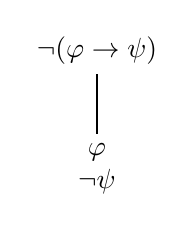
\begin{tikzpicture}[sibling distance=10em,
					every node/.style = {align=center}]
					\node{$\neg(\varphi\to\psi)$}
					child{node{$\varphi$\\$\neg\psi$}};
					\end{tikzpicture}
				\end{center}
		\end{columns}
		\vspace{7pt}
		\hrule
		\vspace{7pt}
		\begin{columns}
			\column{0.1\textwidth}
				\begin{tikzpicture}[sibling distance=10em,
				every node/.style = {align=center}]
				\node{$\varphi\wedge\psi$}
				child{node{$\varphi$\\$\psi$}};
				\end{tikzpicture}
			\column{0.35\textwidth}
				\resizebox{\textwidth}{!}{
					\begin{tikzpicture}[sibling distance=10em,
					every node/.style = {align=center}]
					\node{$\!\!\!\!\neg(\varphi\wedge\psi)$}
					child{node{$\neg\varphi$}}
					child{node{$\neg\psi$}};
					\end{tikzpicture}}
			\column{0.35\textwidth}
				\resizebox{\textwidth}{!}{
					\begin{tikzpicture}[sibling distance=10em,
					every node/.style = {align=center}]
					\node{$\varphi\vee\psi$}
					child{node{$\varphi$}}
					child{node{$\psi$}};
					\end{tikzpicture}}
			\column{0.12\textwidth}
				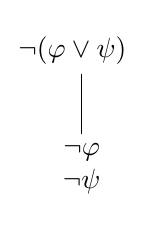
\begin{tikzpicture}[sibling distance=10em,
				every node/.style = {align=center}]
				\node{$\!\!\!\!\neg(\varphi\vee\psi)$}
				child{node{$\neg\varphi$\\$\neg\psi$}};
				\end{tikzpicture}
		\end{columns}
		\vspace{7pt}
		\hrule
		\vspace{7pt}
		\begin{columns}
			\column{0.35\textwidth}\hspace{-7pt}
				\resizebox{\textwidth}{!}{
					\begin{tikzpicture}[sibling distance=10em,
					every node/.style = {align=center}]
					\node{$\varphi\leftrightarrow\psi$}
					child{node{$\varphi$\\$\psi$}}
					child{node{$\neg\varphi$\\$\neg\psi$}};
					\end{tikzpicture}}
			\column{0.35\textwidth}\hspace{-7pt}
				\resizebox{\textwidth}{!}{
					\begin{tikzpicture}[sibling distance=10em,
					every node/.style = {align=center}]
					\node{$\neg(\varphi\leftrightarrow\psi)$}
					child{node{$\varphi$\\$\neg\psi$}}
					child{node{$\neg\varphi$\\$\psi$}};
					\end{tikzpicture}}
		\end{columns}
	\[\textcolor{red}{\checkmark}\]
}

\frame{{Instructions for Tree Construction}
\begin{itemize}
	\item A \emph{literal} is an atomic formula or its negation.
	\item When a non-literal wff has been fully unpacked, check it with $\textcolor{red}{\checkmark}$
\end{itemize}
\begin{enumerate}
	\item Start with premises and the negation of the conclusion.
	\item Inspect each open path for an occurrance of a wff and its negation. If these occur, close the path with $\textcolor{red}{\times}$.
	\item If there is no unchecked non-literal wff on any open path, then stop!
	\item Otherwise, unpack any unchecked non-literal wff on any open path.
	\item Goto \textcircled{\footnotesize 2}.
\end{enumerate}
\begin{itemize}
	\item \emph{Closed branch.} A branch is closed if it contains a wff and its negation.
	\item \emph{Closed tree.} A tree is closed if all its branches are closed.
	\item \emph{Open branch.} A branch is open if it is not closed and no rule can be applied.
	\item \emph{Open tree.} A tree is open if it has at least one open branch.
\end{itemize}
}

\frame{{Tactics}
\begin{itemize}
	\item Try to apply ``non-branching'' rules first, in order to reduce the number of branches.
	\item Try to close off branches as quickly as possible.
\end{itemize}
\begin{definition}[Deduction]
	$\varphi_1,\dots,\varphi_n\vdash\psi$ iff there exists a \emph{closed tree} from $\{\varphi_1,\dots,\varphi_n,\neg\psi\}$.
\end{definition}
\begin{theorem}[Soundness \& Completeness Theorem]
	\[\varphi_1,\dots,\varphi_n\vdash\psi\iff \varphi_1,\dots,\varphi_n\vDash\psi\]
\end{theorem}
	\textbf{Remark:} If an inference with
propositional formulas is not valid, then its tree will have at least one open branch. The tree method can generate every counterexample of an invalid inference in propositional logic.
}

\frame{{Examples --- Tree Method}
\begin{flushright}
	\fbox{$p\to q, \neg q\vee r\vdash\neg p\vee r$}
\end{flushright}
	\begin{center}
		\begin{tikzpicture}[sibling distance=10em,
		every node/.style = {align=center}]
		\node{\quad$p\to q\;\textcolor{red}{\checkmark}$\\\;$\neg q\vee r\;\textcolor{red}{\checkmark}$\\\!\!$\neg(\neg p\vee r)\;\textcolor{red}{\checkmark}$}
		child{node{$\neg\neg p$\\$\neg r$}
			child{node{$\neg p$\\$\textcolor{red}{\times}$}}
			child{node{$q$}
				child{node{$\neg q$\\$\textcolor{red}{\times}$}}
				child{node{$r$\\$\textcolor{red}{\times}$}}}};
		\end{tikzpicture}
	\end{center}
}

\frame{{An open branch corresponds to a valuation}\vspace{-1ex}
\begin{flushright}
	\fbox{$p\vee q, r\vee s, s\to t\stackrel{?}{\vDash} r$}
\end{flushright}
	\begin{center}\vspace{-5ex}
		\begin{tikzpicture}[sibling distance=10em,
		every node/.style = {align=center}]
		\node{\;\;\;$p\vee q\;\textcolor{red}{\checkmark}$\\\;\;\;$r\vee s\;\textcolor{red}{\checkmark}$\\\;\;\;$s\to t\;\textcolor{red}{\checkmark}$\\$\neg r$}
		child{node{$r$\\$\textcolor{red}{\times}$}}
		child{node{$s$}
			child{node{$\neg s$\\$\textcolor{red}{\times}$}}
			child{node{$t$}
				child{node{$p$}}
				child{node{$q$}}}};
		\end{tikzpicture}
	\end{center}
	\[\nu(r)=0,\quad \nu(s)=1,\quad \nu(t)=1\quad \nu(p)=1\quad\nu(q)=1 \mbox{ or } 0\]
	\[\nu(r)=0,\quad \nu(s)=1,\quad \nu(t)=1\quad \nu(q)=1\quad\nu(p)=1 \mbox{ or } 0\]
	\[\nu\vDash p\vee q,\quad \nu\vDash r\vee s,\quad \nu\vDash s\to t,\quad \nu\nvDash r\]
}

{\setbeamercolor{normal text}{fg=fore,bg=back}\usebeamercolor[fg]{normal text}
	\frame{{Exercises --- Tree Method}
		\begin{enumerate}
			\item $p\to(\neg q\to q)\vdash p\to q$
			\item $(p\to r)\wedge(q\to r)\vdash p\vee q\to r$
			\item $(p\to q)\wedge(r\to s)\vdash\neg q\wedge r\to\neg q\wedge s$
			\item $\Big(\big((p\to q)\to(\neg r\to\neg s)\big)\to r\Big)\to t\vdash (t\to p)\to s\to p$
			\item $(p\to q)\vee(q\to r)$
			\item $(p\to q)\to(\neg p\to q)\to q$
			\item $((p\to q)\to p)\to p$
			\item $(p\to q)\wedge(r\to s)\to p\vee r\to q\vee s$
			\item $(p\to q)\wedge r\to\neg(p\wedge r)\vee(q\wedge r)$
			\item $(p\leftrightarrow(p\to q))\to q$
			\item $\neg(p\leftrightarrow q)\leftrightarrow(\neg p\leftrightarrow q)$
		\end{enumerate}
	}
}

{\setbeamercolor{normal text}{fg=fore,bg=back}\usebeamercolor[fg]{normal text}
\frame{{Exercises --- Tree Method}
\textcolor{white}{Decide whether the following inferences are valid or not. If not, provide a counterexample.}
\begin{enumerate}
	\item $(p\vee q)\wedge r\stackrel{?}{\vDash} p\vee(q\wedge r)$
	\item $p\vee(q\wedge r)\stackrel{?}{\vDash} (p\vee q)\wedge r$
	\item $p\leftrightarrow(q\to r)\stackrel{?}{\vDash}(p\leftrightarrow q)\to r$
	\item $(p\leftrightarrow q)\to r\stackrel{?}{\vDash}p\leftrightarrow(q\to r)$
	\item $\neg(p\to q\wedge r),r\to p\wedge q \stackrel{?}{\vDash}\neg r$
	\item $p\to(q\wedge r), \neg(p\vee q\to r)\stackrel{?}{\vDash}p$
	\item $p\to q, r\to s, p\vee r, \neg(q\wedge s)\stackrel{?}{\vDash}(q\to p)\wedge(s\to r)$
	\item If God does not exist, then it's not the case that \emph{if I pray, my prayers will be answered}; and I don't pray; so God exists.
\end{enumerate}
}
}

%---------------------------------%
\subsection{Meta-Theorems}
%---------------------------------%

\frame{{Independence}\vspace{-1ex}
	\setlength\abovedisplayskip{0pt}
	\setlength\belowdisplayskip{0pt}
	\begin{definition}[Independence]
		An axiom $\varphi$ in $\Gamma$ is independent if $\Gamma\setminus\{\varphi\}\nvdash\varphi$.
	\end{definition}
\begin{tcolorbox}
	\textcolor{blue}{找一个这个公理没有的性质,证明能从其他公理推出来的命题都有这个性质。} 比如对某个特殊语义$\Vdash$:
	\begin{itemize}
		\item for all $\psi$, $\Gamma\setminus\{\varphi\}\vdash\psi\implies\Vdash\psi$
		\item $\nVdash\varphi$
	\end{itemize}
\end{tcolorbox}\vspace{-1ex}
	\begin{theorem}
	Axiom$3$ is independent of Axiom$1$ and Axiom$2$.
	\end{theorem}\vspace{-2ex}
\[
\begin{tabu}{c|c}
\hline
p & \neg p\\
\hline
0 & 0\\
1 & 0\\
\hline
\end{tabu}\qquad
\begin{tabu}{c|cc}
\hline
\to & 0 & 1\\
\hline
0 & 1 & 1\\
1 & 0 & 1\\
\hline
\end{tabu}
\]
Let $\nu(p)=0$ and $\nu(q)=1$, then $\nVdash(\neg p\to\neg q)\to(\neg p\to q)\to p$.
}

\frame{{Independence}
Axiom$1$ and Axiom$2$ axiomatizes the conditional ($\to$) fragment of intuitionistic propositional logic. To axiomatize the conditional fragment of classical logic, we also need \emph{Peirce's law}: $((p\to q)\to p)\to p$.
\begin{theorem}
	Peirce's law is independent of Axiom$1$ and Axiom$2$.
	\end{theorem}
\begin{table}
  \begin{tabu}{c|ccc}
    \hline
    $\to$ & 1 & 2 & 3\\
    \hline
    1 & 1 & 2 & 3\\
    2 & 1 & 1 & 3\\
    3 & 1 & 1 & 1\\
    \hline
  \end{tabu}
\end{table}
Here we interpret $1$ as ``true'', $3$ as ``false'', and $2$ as ``maybe''.\\
Let $\nu(p)=2$ and $\nu(q)=3$, then $\nu(((p\to q)\to p)\to p)=2$.
}

\frame{{Model \& Semantic Consequence}
\begin{columns}
\column{.4\textwidth}
	\begin{itemize}
		\item $\mathrm{Mod}(\varphi):=\left\{\nu\colon \nu\vDash\varphi\right\}$
		\item $\mathrm{Mod}(\Gamma):=\bigcap\limits_{\varphi\in\Gamma}\mathrm{Mod}(\varphi)$
		\item $\mathrm{Th}(\nu):=\left\{\varphi\colon \nu\vDash\varphi\right\}$
		\item $\mathrm{Th}(\mathcal{K}):=\bigcap\limits_{\nu\in\mathcal{K}}\mathrm{Th}(\nu)$
		\item $\mathrm{Cn}(\Gamma):=\left\{\varphi\colon \Gamma\vDash\varphi\right\}$
	\end{itemize}
\column{.6\textwidth}
	\begin{tcolorbox}
		\begin{itemize}
			\item \textcolor{blue}{$\Gamma\subset\Gamma'\implies\mathrm{Mod}(\Gamma')\subset\mathrm{Mod}(\Gamma)$}
			\item \textcolor{blue}{$\mathcal{K}\subset\mathcal{K}'\implies\mathrm{Th}(\mathcal{K}')\subset\mathrm{Th}(\mathcal{K})$}
			\item \textcolor{blue}{$\Gamma\subset\mathrm{Th}(\mathrm{Mod}(\Gamma))$}
			\item \textcolor{blue}{$\mathcal{K}\subset\mathrm{Mod}(\mathrm{Th}(\mathcal{K}))$}
			\item $\mathrm{Mod}(\Gamma)=\mathrm{Mod}(\mathrm{Th}(\mathrm{Mod}(\Gamma)))$
			\item $\mathrm{Th}(\mathcal{K})=\mathrm{Th}(\mathrm{Mod}(\mathrm{Th}(\mathcal{K})))$
			\item $\mathrm{Cn}(\Gamma)=\mathrm{Th}(\mathrm{Mod}(\Gamma))$
			\item $\Gamma\subset\Gamma'\implies \mathrm{Cn}(\Gamma)\subset \mathrm{Cn}(\Gamma')$
			\item $\mathrm{Cn}(\mathrm{Cn}(\Gamma))=\mathrm{Cn}(\Gamma)$
		\end{itemize}
	\end{tcolorbox}
\end{columns}
}

\frame{{Consistency \& Satisfiability}
	\begin{itemize}
		\item $\Gamma$ is \textcolor{blue}{consistent} if $\Gamma\nvdash\bot$.
		\item $\Gamma$ is \textcolor{blue}{Post-consistent} if there is some wff $\varphi\colon\Gamma\nvdash\varphi$.
		\begin{center}
			\fbox{$\Gamma$ is consistent iff it is Post-consistent.}
		\end{center}
		\item $\Gamma$ is \textcolor{blue}{maximal} if for every wff $\varphi$, either $\varphi\in\Gamma$ or $\neg\varphi\in\Gamma$.
		\item $\Gamma$ is \textcolor{blue}{maximal consistent} if it is both consistent and maximal.
	\end{itemize}
	\begin{itemize}
		\item $\Gamma$ is \textcolor{blue}{satisfiable} if  $\mathrm{Mod}(\Gamma)\neq\emptyset$.
		\item $\Gamma$ is \textcolor{blue}{finitely satisfiable} if  every finite subset of $\Gamma$ is satisfiable.
	\end{itemize}
	\begin{tcolorbox}
		\begin{itemize}
			\item If $\Gamma$ is consistent and $\Gamma\vdash\varphi$, then $\Gamma\cup\{\varphi\}$ is consistent.
			\item $\Gamma\cup\{\neg\varphi\}$ is inconsistent iff $\Gamma\vdash\varphi$.
			\item {\small If $\Gamma$ is maximal consistent, then $\varphi\notin\Gamma\implies\Gamma\cup\{\varphi\}\;\text{is inconsistent}$.}
		\end{itemize}
	\end{tcolorbox}
}

\frame{{Soundness Theorem}
	\begin{theorem}[Soundness Theorem]
		\[\Gamma\vdash\varphi\implies\Gamma\vDash\varphi\]
	\end{theorem}
	\begin{proof}
		Prove by induction on the length of the deduction sequence.\\
		Case1: $\varphi$ is an axiom. (truth table)\\
		Case2: $\varphi\in\Gamma$\\
		Case3:
		\[\left.
		\begin{aligned}
		\Gamma&\vDash\alpha_j\\
		\Gamma&\vDash\alpha_j\to\varphi
		\end{aligned}\right\}\implies\Gamma\vDash\varphi\]
	\end{proof}
	\begin{corollary}
		Any \textcolor{red}{satisfiable} set of wffs is \textcolor{red}{consistent}.
	\end{corollary}
}

\frame{{Compactness Theorem}
	\setlength\abovedisplayskip{0pt}
	\setlength\belowdisplayskip{0pt}
	\begin{theorem}[Compactness Theorem]
		A set of wffs is satisfiable iff it is finitely satisfiable.
	\end{theorem}
	\begin{tcolorbox}
	如果语言可以说无穷析取,则没有紧致性。$\left\{\bigvee\limits_{i=1}^\infty p_i,\neg p_1,\neg p_2,\dots\right\}$
	\end{tcolorbox}
	\begin{corollary}
		If $\Gamma\vDash\varphi$, then there is a finite $\Gamma_0\subset\Gamma$ s.t. $\Gamma_0\vDash\varphi$.
	\end{corollary}
	\begin{proof}
		\begin{align*}
		\Gamma_0\nvDash\varphi\;\text{for any}\;\Gamma_0\subset\Gamma&\implies\Gamma_0\cup\{\neg\varphi\}\;\text{is satisfiable for any}\;\Gamma_0\subset\Gamma\\
		&\implies\Gamma\cup\{\neg\varphi\}\;\text{is satisfiable}\\
		&\implies\Gamma\nvDash\varphi
		\end{align*}
	\end{proof}
}

\frame{{Applications of Compactness $\stackrel{\rightharpoonup}{\odot}\!\!\underline{\Delta}\!\!\stackrel{\leftharpoonup}{\odot}$}
	\begin{figure}
		\includegraphics[width=\textwidth]{img/4color}
	\end{figure}
	\begin{center}
		\resizebox{\textwidth}{!}{\fbox{An infinite graph $(V,E)$ is $n$-colorable iff every finite subgraph of $(V,E)$ is $n$-colorable.}}
	\end{center}
\begin{proof}
Take $V\times\{1,\dots,n\}$ as the set of atoms.
$\Gamma:=\big\{p(v,1)\vee\dots\vee p(v,n)\colon v\in V\big\}\cup\big\{\neg\big(p(v,i)\wedge p(v,j)\big)\colon v\in V, 1\leq i<j\leq n\big\}\cup\big\{\neg\big(p(v,i)\wedge p(w,i)\big)\colon (v,w)\in E, 1\leq i\leq n\big\}$
\end{proof}
}

\frame{{Proof of Compactness Theorem}
	\begin{proof}
		part1. Extend the finitely satisfiable
		set $\Gamma$ to a maximal finitely satisfiable set $\Delta$.\\
		Let $\left\langle\varphi_i\colon i\in\mathbb{N}\right\rangle$ be a fixed enumeration of the wffs.
		\begin{align*}
		\Delta_0&:=\Gamma\\
		\Delta_{n+1}&:=
		\begin{cases}
		\Delta_n\cup\{\varphi_n\} &\text{if $\Delta_n\cup\{\varphi_n\}$ is finitely satisfiable}\\
		\Delta_n\cup\{\neg\varphi_n\} &\text{otherwise}
		\end{cases}\\
		\Delta&:=\bigcup\limits_{n\in\mathbb{N}}\Delta_n
		\end{align*}
		part2. Define a truth assignment that satisfies $\Gamma$.
		\[\nu(p):=
		\begin{cases}
		1 &\text{if}\; p\in\Delta\\
		0 &\text{otherwise}
		\end{cases}\implies\big(\nu\vDash\varphi\iff \varphi\in\Delta\big)\]
	\end{proof}
}

\frame{{``Compactness Theorem''}
	\begin{theorem}[``Compactness Theorem'']
		$\Gamma$ is consistent iff every finite subset of $\Gamma$ is consistent.
	\end{theorem}
	\begin{proof}
		Suppose $\Gamma\vdash\varphi$ and $\Gamma\vdash\neg\varphi$.\\
		Then there is a deduction sequence $(\alpha_1,\dots,\alpha_n)$ of $\varphi$ from $\Gamma$, and a deduction sequence $(\beta_1,\dots,\beta_m)$ of $\neg\varphi$ from $\Gamma$.\\
		Let $\Sigma_0:=\{\alpha_i\in\Gamma\colon 1\leq i\leq n\}$ and $\Sigma_1:=\{\beta_i\in\Gamma\colon 1\leq i\leq m\}$.\\
		The finite set $\Sigma:=\Sigma_0\cup\Sigma_1$ is inconsistent.
	\end{proof}
}

\frame{{Weak Completeness Theorem}
	\begin{lemma}
		Let $\varphi$ be a wff whose only propositional symbols are $p_1,\dots,p_n$. Let
		\[p_i^\nu:=
		\begin{cases}
		p_i &\text{if}\;\nu\vDash p_i\\
		\neg p_i &\text{otherwise}
		\end{cases}\qquad
		\varphi^\nu:=
		\begin{cases}
		\varphi &\text{if}\;\nu\vDash\varphi\\
		\neg\varphi &\text{otherwise}
		\end{cases}\]
		then $p_1^\nu,\dots,p_n^\nu\vdash\varphi^\nu$.
	\end{lemma}
	\begin{block}{Weak Completeness Theorem\quad \textcolor{red}{$\vDash\varphi\implies\vdash\varphi$}}
		\[\mu(p):=
		\begin{cases}
		1-\nu(p) &\text{if}\;p=p_n\\
		\nu(p) &\text{otherwise}
		\end{cases}
		\]
		\[
		\left.
		\begin{aligned}
		p_1^\nu,\dots,p_{n-1}^\nu,p_n^\nu\vdash\varphi&\\
		p_1^\mu,\dots,p_{n-1}^\mu,p_n^\mu\vdash\varphi&
		\end{aligned}\right\}\implies p_1^\nu,\dots,p_{n-1}^\nu\vdash\varphi
		\]
	\end{block}
}

\frame{{Completeness Theorem}
	\begin{center}
		$\vDash\varphi\iff\;\vdash\varphi\;\;$\\
		$+$\\
		Compactness\\
		$\Downarrow$\\
		$\Gamma\vDash\varphi\iff\Gamma\;\vdash\varphi$
	\end{center}
}

\frame{{Completeness Theorem --- Post1921}
		\begin{theorem}[Completeness Theorem]
			\[\Gamma\vDash\varphi\implies\Gamma\vdash\varphi\]
		\end{theorem}
		\begin{corollary}
			Any \textcolor{red}{consistent} set of wffs is \textcolor{red}{satisfiable}.
		\end{corollary}
		\begin{center}
			\begin{minipage}{.5\textwidth}\vspace{-0.5cm}
				{\Large \[\arraycolsep=0.7pt\def\arraystretch{1.7}
					\begin{array}{cccc}
					&\Gamma\vDash\varphi&\iff&\Gamma\vdash\varphi\\
					&\rotatebox[origin=C]{90}{$\iff$}&&\rotatebox[origin=C]{90}{$\iff$}\\
					&\Gamma\cup\{\neg\varphi\}\atop{\text{unsatisfiable}}&\iff&\Gamma\cup\{\neg\varphi\}\atop{\text{inconsistent}}
					\end{array}
					\]}
			\end{minipage}
		\end{center}\vspace{-3ex}
		\begin{corollary}[Compactness Theorem]
			A set of wffs is satisfiable iff it is finitely satisfiable.
		\end{corollary}
}

\frame{{Proof of Completeness Theorem}
	\begin{proof}
		step$1$. Extend the consistent set $\Gamma$ to a maximal consistent set $\Delta$.\\
		Let $\left\langle\varphi_i\colon i\in\mathbb{N}\right\rangle$ be a fixed enumeration of the wffs.
		\begin{align*}
		\Delta_0&:=\Gamma\\
		\Delta_{n+1}&:=
		\begin{cases}
		\Delta_n\cup\{\varphi_n\} &\text{if $\Delta_n\cup\{\varphi_n\}$ is consistent}\\
		\Delta_n\cup\{\neg\varphi_n\} &\text{otherwise}
		\end{cases}\\
		\Delta&:=\bigcup\limits_{n\in\mathbb{N}}\Delta_n
		\end{align*}
		step$2$. Define a truth assignment that satisfies $\Gamma$.
		\[\nu(p):=
		\begin{cases}
		1 &\text{if}\; p\in\Delta\\
		0 &\text{otherwise}
		\end{cases}\implies\big(\nu\vDash\varphi\iff \varphi\in\Delta\big)\]
	\end{proof}
}

\frame{{Decidability --- Post1921}
	\begin{theorem}
		There is an effective procedure that, given any expression, will decide whether or not it is a wff.
	\end{theorem}
	\begin{theorem}
		There is an effective procedure that, given a finite set $\Gamma\cup\{\varphi\}$ of wffs, will decide whether or not $\Gamma\vDash\varphi$.
	\end{theorem}
	\begin{theorem}
		If $\Gamma$ is a decidable set of wffs, then the set of logical consequences of $\Gamma$ is recursively enumerable.
	\end{theorem}
}

\frame{{Post 1897-1954}
\begin{columns}
\column{.4\textwidth}
\begin{figure}
	\includegraphics[height=.9\textwidth,angle=0,origin=c]{img/post}
\end{figure}
\column{.6\textwidth}
\begin{itemize}
	\item Truth table
	\item Completeness of propositional logic
	\item Post machine
	\item Post canonical system
	\item Post correspondence problem
	\item Post problem
\end{itemize}
\end{columns}
}

\frame{{Theory \& Axiomatization}
	\begin{tcolorbox}[colback=cyan!3,colframe=back!85]
		\centering\textcolor{red}{什么是“理论”?}
	\end{tcolorbox}
	\begin{itemize}
		\item A set $\Gamma$ of sentences is a \textcolor{blue}{theory} if $\Gamma=\mathrm{Cn}(\Gamma)$.
		\item A theory $\Gamma$ is \textcolor{blue}{complete} if for every sentence $\varphi$, either $\varphi\in\Gamma$ or $\neg\varphi\in\Gamma$.
		\item A theory $\Gamma$ is \textcolor{blue}{axiomatizable} if there is a decidable set $\Sigma$ of sentences s.t. $\Gamma=\mathrm{Cn}(\Sigma)$.
		\item A theory $\Gamma$ is \textcolor{blue}{finitely axiomatizable} if $\Gamma=\mathrm{Cn}(\Sigma)$ for some finite set $\Sigma$ of sentences.
	\end{itemize}
}

\frame{{\small Model Checking \& Satisfiability Checking \& Validity Checking\footnote{\tiny \href{https://www.scottaaronson.com/papers/philos.pdf}{Aaronson: Why Philosophers Should Care About Computational Complexity.}}}
	\begin{itemize}
		\item Given a model $\nu$ and a formula $\varphi$. Is $\nu\vDash\varphi$?\hfill ---\textcolor{blue}{P}
		\item Given a formula $\varphi$. Is there a model $\nu$ s.t. $\nu\vDash\varphi$?\hfill ---\textcolor{blue}{NP}
		\item Given a sentence $\varphi$. Is $\vDash\varphi$?
	\end{itemize}
	\begin{columns}
		\column{0.28\textwidth}
			\begin{figure}
				\centering\includegraphics[width=\textwidth]{img/euler-bridge}\\
				\centering\includegraphics[width=\textwidth]{img/eulerian-path}\caption{\tiny{\textit{Eulerian Circle(P)}}}
			\end{figure}
		\column{0.3\textwidth}\vspace{-0.3cm}
			\begin{figure}
				\centering\includegraphics[width=0.7\textwidth]{img/hamiltonian-path}\vspace{-0.2cm}\caption{\tiny{\textit{Hamiltonian Circle(NPC)}}}\vspace{-0.2cm}
				\centering\includegraphics[width=0.7\textwidth]{img/graph-coloring}\vspace{-0.3cm}\caption{\tiny{\textit{Graph Coloring(NPC)}}}
			\end{figure}
		\column{0.4\textwidth}\vspace{-0.5cm}
			\begin{center}
				\begin{figure}
					\includegraphics[width=\textwidth]{img/hanoi.pdf}
				\end{figure}
			\end{center}
	\end{columns}
}

%%%%%%%%%%%%%%%%%%%%%%%%%%%%%%
\subsection{Application}
%%%%%%%%%%%%%%%%%%%%%%%%%%%%%%

\frame{{Information Update}
\begin{center}
\begin{figure}
\includegraphics[width=.6\textwidth]{img/bar}
\end{figure}
\end{center}
The information content of a formula $\varphi$ is the set $\mathrm{Mod}(\varphi)$ of its models. An update with new information $\psi$ reduces the current set of models $\mathrm{Mod}(\varphi)$ to the overlap of $\mathrm{Mod}(\varphi)$ and $\mathrm{Mod}(\psi)$.
}

\frame{{Party and Friends}
	\begin{problem}
		\begin{itemize}
			\item We want to throw a party for \textcolor{blue}{Tweety}, \textcolor{blue}{Gentoo} and \textcolor{blue}{Tux}.
			\item But they have different circles of friends and dislike some.
			\item Tweety tells you that he would like to see \emph{either} his friend \textcolor{blue}{Kimmy} \emph{or} not to meet Gentoo's \textcolor{blue}{Alice}, but not both.
			\item But Gentoo proposes to invite  \textcolor{blue}{Alice} or \textcolor{blue}{Harry} or both.
			\item Tux, however, does not like \textcolor{blue}{Harry} and \textcolor{blue}{Kimmy} too much, so he suggests to \textcolor{blue}{exclude} at least one of them.
		\end{itemize}
	\end{problem}\pause
	\begin{solution}
		\[(K\vee\neg A)\wedge\neg(K\wedge\neg A)\wedge(A\vee H)\wedge(\neg H\vee\neg K)\]
	\end{solution}
}

\frame{{Sudoku}
\begin{columns}
\column{.37\textwidth}
\begin{center}
\resizebox{\textwidth}{!}{$
\begin{tabu}{!{\vrule width2pt}c|c|c!{\vrule width2pt}c|c|c!{\vrule width2pt}c|c|c!{\vrule width2pt}}
\Xhline{2pt}
&&&&&&&&\\
\hline
&\textcolor{red}{\bm{8}}&\textcolor{red}{\bm{6}}&&&&\textcolor{red}{\bm{2}}&\textcolor{red}{\bm{9}}&\\
\hline
\textcolor{red}{\bm{4}}&&&\textcolor{red}{\bm{1}}&&\textcolor{red}{\bm{5}}&&&\textcolor{red}{\bm{8}}\\
\Xhline{2pt}
\textcolor{red}{\bm{7}}&&&&\textcolor{red}{\bm{9}}&&&&\textcolor{red}{\bm{4}}\\
\hline
\textcolor{red}{\bm{1}}&&&&&&&&\textcolor{red}{\bm{9}}\\
\hline
&\textcolor{red}{\bm{5}}&&&&&&\textcolor{red}{\bm{1}}&\\
\Xhline{2pt}
&&\textcolor{red}{\bm{8}}&&&&\textcolor{red}{\bm{3}}&&\\
\hline
&&&\textcolor{red}{\bm{5}}&&\textcolor{red}{\bm{9}}&&&\\
\hline
&&&&\textcolor{red}{\bm{2}}&&&&\\
\Xhline{2pt}
\end{tabu}
$}
\end{center}
\centering\textcolor{blue}{$p(i,j,n):=$ the cell in row $i$ and column $j$ contains the number $n$}
\column{.63\textwidth}
\begin{itemize}
				\item Every row/column contains every number.
				\[\bigwedge\limits_{i=1}^9\bigwedge\limits_{n=1}^9\bigvee\limits_{j=1}^9 p(i,j,n)\qquad\bigwedge\limits_{j=1}^9\bigwedge\limits_{n=1}^9\bigvee\limits_{i=1}^9 p(i,j,n)\]
				\item Every $3\times3$ block contains every number.
				\[\bigwedge\limits_{r=0}^2\bigwedge\limits_{s=0}^2\bigwedge\limits_{n=1}^9\bigvee\limits_{i=1}^3\bigvee\limits_{j=1}^3 p(3r+i,3s+j,n)\]
				\item No cell contains more than one number.
				
				for all $1\leq i,j,n,n'\leq 9$ and $n\neq n'$: \[p(i,j,n)\to\neg p(i,j,n')\]
\end{itemize}
\end{columns}
}

\frame{{Shannon --- Digital Circuit Design}
	\begin{figure}[!htbp]
		\begin{center}
			\includegraphics[width=0.8\textwidth,angle=0,origin=c]{img/circuit1}
		\end{center}
	\end{figure}
	\[(A\wedge B)\vee((C\vee A)\wedge\neg B)\logeq A\vee(C\wedge\neg B)\]
	\begin{figure}[!htbp]
		\begin{center}
			\includegraphics[width=0.8\textwidth,angle=0,origin=c]{img/circuit2}
		\end{center}
	\end{figure}
}

\frame{{Shannon --- Digital Circuit Design}
\begin{figure}
\includegraphics[width=.9\textwidth]{img/boole-circuit.pdf}
\end{figure}
\[(A\vee\neg C)\wedge(B\vee\neg C)\logeq(A\wedge B)\vee\neg C\]
}

\frame{{McCulloch-Pitts Artificial Neural Network}
	\begin{columns}\hspace{-1cm}
		\column{.6\textwidth}
			\resizebox{\textwidth}{!}{
				\begin{minipage}{\textwidth}
					\begin{tikzpicture}
					\node[rectangle, blue, ultra thick, fill=red, opacity=1,label=above:{\parbox{2cm}{\centering activation \\ function}}] at (2,-2)  (sigmoid) {\huge $g$};
					\node[darkgreen,label=above:{\parbox{2cm}{\centering output}}] at (4,-2)  (output) {$y$};
					%%Create a style for the arrows we are using
					\tikzset{normal arrow/.style={draw,-triangle 45,very thick}}
					%%Create the different coordinates to place the nodes
					\path (0,0) coordinate (1) ++(0,-2) coordinate (2) ++(0,-2) coordinate (3);
					\path (1) ++(-2,-1) coordinate (x1);
					\path (3) ++(-2,1) coordinate (x2);
					%%Place nodes at each point using the foreach construct
					\node[draw,circle,shading=axis,top color=green!1, bottom color=green,shading angle=5] at (2) (n2) {$\sum$};
					\node[above of=n2,above=.5cm,label=above:{\parbox{2cm}{\centering bias}}] (b) {$1$};
					\node[below of=n2,below=1ex] {linear};
					\node[below of=sigmoid,below=1ex] {nonlinear};
					\node[left of=n2,left=.2cm] (vdots) {\textcolor{cyan}{\huge $\vdots$}};
					%%Place the remaining nodes separately
					\node[label=above:{\parbox{2cm}{$\;\,$ inputs}}] (nx1) at (x1) {$x_1$};
					\node (nx2) at (x2) {$x_n$};
					%\node (ny)  at (7)  {$y$};
					\path[normal arrow,cyan] (b) -- node[right=.05em,cyan] {$b$} (n2);
					\path[normal arrow,cyan] (n2) --  (sigmoid);
					\path[normal arrow,cyan] (sigmoid) --  (output);
					\path[normal arrow,cyan] (nx1) -- node[label=above:{\parbox{2cm}{\centering\small \textcolor{black}{weights}}}][above=.3em,cyan](w1) {$w_1$} (n2);
					\path[normal arrow,cyan] (nx2) -- node[below=.3em,cyan] {$w_n$} (n2);
					\end{tikzpicture}
			\end{minipage}}
			{\Large \[y=g\left(\sum\limits_{i=1}^n w_ix_i+b\right)\]}
		\column{.4\textwidth}
			\resizebox{.8\textwidth}{!}{
				\begin{minipage}{\textwidth}
					\begin{tikzpicture}
					\node[blue, rectangle, fill=red, opacity=1] at (2,-2)  (sigmoid) {$\chi_{\geq 0}$};
					\node[darkgreen] at (4,-2)  (and) {\Huge{$\wedge$}};
					%%Create a style for the arrows we are using
					\tikzset{normal arrow/.style={draw,-triangle 45,very thick}}
					%%Create the different coordinates to place the nodes
					\path (0,0) coordinate (1) ++(0,-2) coordinate (2) ++(0,-2) coordinate (3);
					\path (1) ++(-2,-1) coordinate (x1);
					\path (3) ++(-2,1) coordinate (x2);
					%%Place nodes at each point using the foreach construct
					\node[draw,circle,shading=axis,top color=green!1, bottom color=green,shading angle=5] at (2) (n2) {$\sum$};
					\node[above of=n2,above=.5cm] (b) {$1$};
					%%Place the remaining nodes separately
					\node (nx1) at (x1) {$x_1$};
					\node (nx2) at (x2) {$x_2$};
					%\node (ny)  at (7)  {$y$};
					\path[normal arrow,cyan] (b) -- node[right=.05em,cyan] {$-2$} (n2);
					\path[normal arrow,cyan] (n2) --  (sigmoid);
					\path[normal arrow,cyan] (sigmoid) --  (and);
					\path[normal arrow,cyan] (nx1) -- node[above=.5em,cyan] {$+1$} (n2);
					\path[normal arrow,cyan] (nx2) -- node[below=.5em,cyan] {$+1$} (n2);
					\end{tikzpicture}
			\end{minipage}}\\
			\resizebox{.8\textwidth}{!}{
				\begin{minipage}{\textwidth}\vspace{-.5cm}
					\begin{tikzpicture}
					\node[blue, rectangle, fill=red, opacity=1] at (2,-2)  (sigmoid) {$\chi_{\geq 0}$};
					\node[darkgreen] at (4,-2)  (or) {\Huge{$\vee$}};
					%%Create a style for the arrows we are using
					\tikzset{normal arrow/.style={draw,-triangle 45,very thick}}
					%%Create the different coordinates to place the nodes
					\path (0,0) coordinate (1) ++(0,-2) coordinate (2) ++(0,-2) coordinate (3);
					\path (1) ++(-2,-1) coordinate (x1);
					\path (3) ++(-2,1) coordinate (x2);
					\node[draw,circle,shading=axis,top color=green!1, bottom color=green,shading angle=5] at (2) (n2) {$\sum$};
					\node[above of=n2,above=.5cm] (b) {$1$};
					%%Place the remaining nodes separately
					\node (nx1) at (x1) {$x_1$};
					\node (nx2) at (x2) {$x_2$};
					%\node (ny)  at (7)  {$y$};
					\path[normal arrow,cyan] (b) -- node[right=.05em,cyan] {$-1$} (n2);
					\path[normal arrow,cyan] (n2) --  (sigmoid);
					\path[normal arrow,cyan] (sigmoid) --  (or);
					\path[normal arrow,cyan] (nx1) -- node[above=.5em,cyan] {$+1$} (n2);
					\path[normal arrow,cyan] (nx2) -- node[below=.5em,cyan] {$+1$} (n2);
					\end{tikzpicture}
			\end{minipage}}\\
			\resizebox{.8\textwidth}{!}{
				\begin{minipage}{\textwidth}\vspace{-.5cm}
					\begin{tikzpicture}
					\node[blue, rectangle, fill=red, opacity=1] at (2,-2)  (sigmoid) {$\chi_{\geq 0}$};
					\node[darkgreen] at (4,-2)  (not) {\Huge{$\neg$}};
					%%Create a style for the arrows we are using
					\tikzset{normal arrow/.style={draw,-triangle 45,very thick}}
					%%Create the different coordinates to place the nodes
					\path (0,0) coordinate (1) ++(0,-2) coordinate (2) ++(0,-2) coordinate (3);
					\path (1) ++(-2,-2) coordinate (x1);
					%%Place nodes at each point using the foreach construct
					\node[draw,circle,shading=axis,top color=green!1, bottom color=green,shading angle=5] at (2) (n2) {$\sum$};
					\node[above of=n2,above=.5cm] (b) {$1$};
					%%Place the remaining nodes separately
					\node (nx1) at (x1) {$x$};
					%\node (ny)  at (7)  {$y$};
					\path[normal arrow,cyan] (b) -- node[right=.05em,cyan] {$0$} (n2);
					\path[normal arrow,cyan] (n2) --  (sigmoid);
					\path[normal arrow,cyan] (sigmoid) --  (not);
					\path[normal arrow,cyan] (nx1) -- node[above=.5em,cyan] {$-1$} (n2);
					\end{tikzpicture}
			\end{minipage}}
	\end{columns}
}

\frame{{}
\begin{tcolorbox}[title=《三体》]
\begin{itemize}
	\item 秦始皇:朕当然需要预测太阳的运行,但你们让我集结三千万大军,至少要首先向朕演示一下这种计算如何进行吧。
	\item 冯诺依曼:陛下,请给我三个士兵,我将为您演示。……
	\item 秦始皇:他们不需要学更多的东西了吗?
	\item 冯诺依曼:不需要,我们组建一千万个这样的门部件,再将这些部件组合成一个系统,这个系统就能进行我们所需要的运算,解出那些预测太阳运行的微分方程。
\end{itemize}
\end{tcolorbox}
\begin{columns}	
\column{0.3\textwidth}
	\begin{table}
		\begin{tabu}{cc|c}
			\hline
			\textcolor{red}{p} & \textcolor{red}{q} & $p\dot{\vee}q$\\
			\hline
			0 & 0  & 0\\
			0 & 1  & 1\\
			1 & 0  & 1\\
			1 & 1  & 0\\
			\hline
		\end{tabu}
	\end{table}
\column{0.4\textwidth}
\begin{align*}
w_1\cdot 0+w_2\cdot 0+b<0\\
w_1\cdot 0+w_2\cdot 1+b\geq 0\\
w_1\cdot 1+w_2\cdot 0+b\geq 0\\
w_1\cdot 1+w_2\cdot 1+b<0
\end{align*}
\column{0.3\textwidth}
\begin{align*}
b<0\\
w_2+b\geq 0\\
w_1+b\geq 0\\
w_1+w_2+b<0
\end{align*}
\end{columns}
A simple single-layer perception can't solve nonlinearly separable problems.
}

\frame{{Finite State Automaton}
\begin{columns}
\column{.5\textwidth}
\begin{figure}[H]
\includegraphics[width=\textwidth]{img/boole-automata.pdf}
\end{figure}
\column{.5\textwidth}
\[
\begin{tabu}{ccc|cc}
\hline
y_1&y_2&x&y_1^+&y_2^+\\
\hline
0 & 0 & 0 & 1 & 0 \\
0 & 0 & 1 & 1 & 0 \\
0 & 1 & 0 & 0 & 0 \\
0 & 1 & 1 & 0 & 0 \\
1 & 0 & 0 & 1 & 1 \\
1 & 0 & 1 & 0 & 1 \\
1 & 1 & 0 & 0 & 0 \\
1 & 1 & 1 & 0 & 1 \\
\hline
\end{tabu}
\]
\end{columns}
\begin{align*}
y_1^+&=\bar{y}_1\bar{y}_2+\bar{x}\bar{y}_2\\
y_2^+&=y_1\bar{y}_2+xy_1
\end{align*}
}

\frame{{Reversible Computing --- Fredkin Gate}
\begin{columns}
\column{.38\textwidth}
\begin{tabular}{lll|lll}
\hline
$c$   & $x_1$  &$x_2$&$c'$&$y_1$&$y_2$\\
\hline
0     & 0      & 0  & 0 & 0  & 0  \\
0     & 0      & 1  & 0 & 0  & 1  \\
0     & 1      & 0  & 0 & 1  & 0  \\
0     & 1      & 1  & 0 & 1  & 1  \\
1     & 0      & 0  & 1 & 0  & 0  \\
1     & 0      & 1  & 1 & 1  & 0  \\
1     & 1      & 0  & 1 & 0  & 1  \\
1     & 1      & 1  & 1 & 1  & 1  \\
\hline
\end{tabular}
\column{.6\textwidth}
\begin{figure}[H]
\includegraphics[width=\textwidth]{img/fredkin-gate.pdf}\caption{transmit the first bit unchanged and swap the last two bits iff the first bit is $1$. $f\colon(c,x_1,x_2)\mapsto(c,\bar{c}x_1+cx_2,cx_1+\bar{c}x_2)$}
\end{figure}
\end{columns}
\begin{columns}
\column{.65\textwidth}
\begin{itemize}
\item If $x_2 = 0$, then $y_2 = cx_1$.\hfill$\wedge$
\item If $x_2 = 1$, then $y_1 = c+x_1$.\hfill$\vee$
\item If $x_1 = 0$ and $x_2 = 1$, then $y_2 = \bar{c}$.\hfill$\neg$
\end{itemize}
\end{columns}
}

\frame{{Exercise}
\begin{tcolorbox}[colback=cyan!3,colframe=back!85,title=宝藏在哪里?]
你面前有三扇门,只有一扇门后是宝藏。门上各有一句话,只有一扇门上的是真话。
\begin{enumerate}
	\item 宝藏不在这儿。
	\item 宝藏不在这儿。
	\item 宝藏在\textcircled{\footnotesize 2}号门。
\end{enumerate}
\end{tcolorbox}
\begin{itemize}
	\item \textcircled{\footnotesize 1} $\neg t_1$; \textcircled{\footnotesize 2} $\neg t_2$; \textcircled{\footnotesize 3} $t_2$.
	\item 只有一扇门上的是真话。
	$(\neg t_1\wedge\neg\neg t_2\wedge\neg t_2)\vee(\neg\neg t_1\wedge\neg t_2\wedge\neg t_2)\vee(\neg\neg t_1\wedge\neg\neg t_2\wedge t_2)$
	\item 只有一扇门后是宝藏。\\
	$(t_1\wedge\neg t_2\wedge\neg t_3)\vee(\neg t_1\wedge t_2\wedge\neg t_3)\vee(\neg t_1\wedge\neg t_2\wedge t_3)$
\end{itemize}
}

{\setbeamercolor{normal text}{bg=back}
	\frame{{Exercise}
		\begin{tcolorbox}[colback=cyan!3,colframe=back!85,title=谁是凶手?]
			一起凶杀案有三个嫌疑人:小白、大黄和老王。
			\begin{enumerate}
				\item 至少有一人是凶手,但不可能三人同时犯罪。
				\item 如果小白是凶手,那么老王是同犯。
				\item 如果大黄不是凶手,那么老王也不是。
			\end{enumerate}
		\end{tcolorbox}
		\begin{tcolorbox}[colback=cyan!3,colframe=back!85,title=谁是窃贼?]
			\begin{enumerate}
				\item 钱要么是甲偷的要么是乙偷的。
				\item 如果是甲偷的,则偷窃时间不会在午夜前。
				\item 如果乙的证词正确,则午夜时灯光未灭。
				\item 如果乙的证词不正确,则偷窃发生在午夜前。
				\item 午夜时没有灯光。
			\end{enumerate}
		\end{tcolorbox}
	}
}

{\setbeamercolor{normal text}{bg=back}
	\frame{{Exercise}
		\begin{tcolorbox}[colback=cyan!3,colframe=back!85,title=哪个部落的?]
		一个岛上有T、F两个部落,T部落的居民只说真话,F部落的居民只说谎。你在岛上遇到了小白、大黄、老王三个土著。
			\begin{enumerate}
				\item 小白:“如果老王说谎,我或大黄说的就是真话”。
				\item 大黄:“只要小白或老王说真话,那么,我们三人中有且只有一人说真话是不可能的”。
				\item 老王:“小白或大黄说谎当且仅当小白或我说真话”。
			\end{enumerate}
		\end{tcolorbox}
		\begin{tcolorbox}[colback=cyan!3,colframe=back!85,title=我在做什么?]
			\begin{enumerate}
				\item 如果我不在打网球,那就在看网球。
				\item 如果我不在看网球,那就在读网球杂志。
				\item 但我不能同时做两件以上的事。
			\end{enumerate}
		\end{tcolorbox}
	}
}

\frame{{Summary}
	\begin{itemize}
		\item Syntax
		\item Semantics
		\item Formal System
	\end{itemize}
	\begin{itemize}
		\item Expressiveness / Succinctness
		\item Satisfiability / Validity
		\item Soundness / Completeness / Compactness
		\item Decidability / Computational Complexity
		\item $\phantom{Dec}\vdots$
	\end{itemize}
}


%%%%%%%%%%%%%%%%%%%%%%%%%%%%%%%
\section{Predicate Logic}
%%%%%%%%%%%%%%%%%%%%%%%%%%%%%%%


\frame{{Why Study Predicate Logic?}
	\begin{itemize}
		\item Propositional logic assumes the world contains \textcolor{red}{facts}.
		\item Predicate logic assumes the world contains
		\begin{itemize}
			\item \textcolor{red}{Objects}: people, houses, numbers, colors, baseball games, wars, \dots
			\item \textcolor{red}{Relations}: red, round, prime, brother of, bigger than, part of, between, fall in love with, \dots
			\item \textcolor{red}{Functions}: father of, best friend, one more than, plus, \dots
		\end{itemize}
		\item Expressive power.
	\end{itemize}
}

\frame{{Example}
	\begin{block}{$\sideset{^\circledcirc}{^\circledcirc}{\mathop{\hat{o}}}$}
		What will a logician choose: an egg or eternal bliss in the afterlife? An egg! Because nothing is better than eternal bliss in the afterlife, and an egg is better than nothing.
	\end{block}
	\[b<0<e\implies b<e\]
	\[\neg\exists x(x>b)\implies 0\ngtr b\]
	\begin{block}{$\sideset{^\circledcirc}{^\circledcirc}{\mathop{\hat{o}}}$}
		No cat has eight tails. A cat has one tail more than no cat. Therefore, a cat has nine tails.
	\end{block}
}

\frame{{}
	\begin{figure}
		\includegraphics[width=0.93\textwidth,angle=0,origin=c]{img/mathtree}
	\end{figure}
}

\frame{{}
	\begin{figure}
		\includegraphics[width=0.8\textwidth,angle=-90,origin=c]{img/tree}
	\end{figure}
}

\frame{{}
	\begin{figure}
		\includegraphics[width=0.6\textwidth,angle=0,origin=c]{img/theory-tree}
	\end{figure}
}

\frame{{打破学科鄙视链}
	\begin{figure}
		\includegraphics[width=\textwidth,angle=0,origin=c]{img/purity}\caption{还原论 $\ne$ 演生论}
	\end{figure}
}

%%%%%%%%%%%%%%%%%%%%
\subsection{Syntax}
%%%%%%%%%%%%%%%%%%%%

\frame{{Syntax}
		\begin{block}{Language}
			\[\mathscr{L}^1:=\{\textcolor{darkgreen}{\neg},\wedge,\vee,\textcolor{darkgreen}{\to},\leftrightarrow,\textcolor{darkgreen}{\forall},\exists,=,(,)\}\cup\mathscr{V}\cup\overbrace{\textcolor{blue}{\mathscr{F}}\cup\textcolor{blue}{\mathscr{Q}}}^{\text{signature}}\]
		\end{block}
		where
		\[\mathscr{V}:=\{x_i\colon i\in\mathbb{N}\}\]
		\[\mathscr{F}:=\bigcup\limits_{k\in\mathbb{N}}\mathscr{F}^k\quad \mathscr{F}^k:=\left\{f_1^k,\dots,f_n^k,(\dots)\right\}\]
		\[\mathscr{Q}:=\bigcup\limits_{k\in\mathbb{N}}\mathscr{Q}^k\quad \mathscr{Q}^k:=\left\{P_1^k,\dots,P_n^k,(\dots)\right\}\]
		$f^k$ is a $k$-place function symbol.\\
		$P^k$ is a $k$-place predicate symbol.\\
		A $0$-place function symbol $f^0$ is called constant.\\
		A $0$-place predicate symbol $P^0$ is called (atomic) proposition.
}

\frame{{Term \& Formula}
		\begin{block}{Term $\mathcal{T}$}
			\[t::= x\mid f(t,\dots,t)\]
			where $x\in\mathscr{V}$ and $f\in\mathscr{F}$.
		\end{block}
		\begin{itemize}
			\item $\mathcal{T}$ is freely generated from $\mathscr{V}$ by $\mathscr{F}$.
		\end{itemize}
		\begin{block}{Well-Formed Formula $\mathrm{WFF}$}
			\[\varphi::=\overbrace{\textcolor{purple}{t=t}\mid \textcolor{purple}{P(t,\dots,t)}}^{\text{atomic formula}}\mid \textcolor{darkgreen}{\neg\varphi}\mid \varphi\wedge\psi\mid \varphi\vee\psi\mid \textcolor{darkgreen}{\varphi\to\varphi}\mid \varphi\leftrightarrow\psi\mid \textcolor{darkgreen}{\forall x\varphi}\mid \exists x\varphi\]
			where $t\in\mathcal{T}$ and $P\in\mathscr{Q}$.
		\end{block}
		\begin{itemize}
			\item $\mathrm{WFF}$ is freely generated from atomic formulas by connective and quantifier operators.
		\end{itemize}
}

\frame{{Syntax}
\centering\begin{minipage}{.6\textwidth}
	\begin{tcolorbox}
		\begin{itemize}
			\item $\varphi\wedge\psi:=\neg(\varphi\to\neg\psi)$
			\item $\varphi\vee\psi:=\neg\varphi\to\psi$
			\item $\varphi\leftrightarrow\psi:=(\varphi\to\psi)\wedge(\psi\to\varphi)$
			\item $\exists x\varphi:=\neg\forall x\neg\varphi$
			\item $\bot:=\varphi\wedge\neg\varphi$
			\item $\top:=\neg\bot$
		\end{itemize}
	\end{tcolorbox}
\end{minipage}
	\begin{itemize}
		\item Bottom up and Top down definitions of terms, subterms, wffs and subformulas.
		\item Induction Principle for terms and wffs.
		\item Unique readability theorem for terms and wffs.
		\item Omitting Parenthesis.\\
		\small{1). outermost parentheses. 2).  $\neg,\forall,\exists,\wedge,\vee,\to,\leftrightarrow$ 3). group to the right.}
	\end{itemize}
}

\frame{{Freedom \& Bondage}
	\begin{columns}
		\column{.5\textwidth}
			\[\exists\textcolor{blue}{y}\forall\textcolor{darkgreen}{z}(\neg\exists \textcolor{red}{x} R\textcolor{red}{x}\textcolor{darkgreen}{z}\to Rx\textcolor{blue}{y}\wedge R\textcolor{darkgreen}{z}\textcolor{cyan}{c})\]
			\centering\tikz[level distance=10mm,outer sep=1mm,inner sep=0,
			level 1/.style={sibling distance=20mm},
			level 2/.style={sibling distance=35mm},
			level 3/.style={sibling distance=30mm},
			level 4/.style={sibling distance=17mm},
			level 5/.style={sibling distance=8mm},
			level 6/.style={sibling distance=8mm}
			]
			\node {$\exists \textcolor{blue}{y}$}
			child {node {$\forall \textcolor{darkgreen}{z}$}
				child {node   {$\to$}
					child {node {$\neg$}
						child{node {$\exists \textcolor{red}{x}$}
							child {node {$R$}
								child {node {$\textcolor{red}{x}$} }
								child {node {$\textcolor{darkgreen}{z}$} }
							}
						}
					}
					child {node  {$\wedge$}
						child {node {$R$}
							child {node {$x$} }
							child {node {$\textcolor{blue}{y}$} }
						}
						child {node {$R$}
							child {node {$\textcolor{darkgreen}{z}$ }}
							child {node {$\textcolor{cyan}{c}$} }
						}
					}
				}
			};
		\column{.52\textwidth}
			\[\sum\limits_{\textcolor{red}{n}=1}^\infty\frac{1}{\textcolor{red}{n}^{\textcolor{blue}{s}}}=\prod\limits_{\textcolor{red}{p}\in\mathbb{P}}\frac{1}{1-\frac{1}{\textcolor{red}{p}^{\textcolor{blue}{s}}}}\]
			\[\mathrm{e}^{\mathrm{i}\theta}=\cos\theta+\mathrm{i}\sin\theta\]
			\[\hspace{-3ex}\left(\sum\limits_{x\in\mathcal{X}}\left|P(x)-Q(x)\right|\right)^2\leq 2\sum\limits_{x\in\mathcal{X}} P(x)\ln \dfrac{P(x)}{Q(x)}\]
			\[\dfrac{\mathrm{d}}{\mathrm{d}x}\int_{a}^x\!\!f(t)\mathrm{d}t=f(x)\]
			\[\int_0^t\!\!\frac{1}{\sqrt{2\pi}}\mathrm{e}^{-\frac{x^2}{2}}\mathrm{d}x\]
			\[f(x)=\sum\limits_{n=1}^\infty\dfrac{f^{(n)}(a)}{n!}(x-a)^n\]
			\[\hat{f}(\xi)=\int_{-\infty}^{\infty}\!\!f(x)\mathrm{e}^{-2\pi \mathrm{i}x\xi}\mathrm{d}x\]
	\end{columns}
}

\frame{{Freedom \& Bondage}
	\begin{definition}[Free Variable of a Term]
		\[
		\mathrm{Fv}(t):=
		\begin{cases}
		x &\text{if}\;t=x\\
		\emptyset &\text{if}\;t=c\\
		\mathrm{Fv}(t_1)\cup\dots\cup \mathrm{Fv}(t_n) &\text{if}\;t=f(t_1,\dots,t_n)
		\end{cases}
		\]
	\end{definition}
	\begin{definition}[Free Variable of a wff]
		\[
		\mathrm{Fv}(\varphi):=
		\begin{cases}
		\mathrm{Fv}(t_1)\cup \mathrm{Fv}(t_2) &\text{if}\;\varphi=t_1= t_2\\
		\mathrm{Fv}(t_1)\cup\dots\cup \mathrm{Fv}(t_n) &\text{if}\;\varphi=P(t_1,\dots,t_n)\\
		\mathrm{Fv}(\psi) &\text{if}\;\varphi=\neg\psi\\
		\mathrm{Fv}(\psi)\cup \mathrm{Fv}(\chi) &\text{if}\;\varphi=\psi\to\chi\\
		\mathrm{Fv}(\psi)\setminus\{x\} &\text{if}\;\varphi=\forall x\psi
		\end{cases}
		\]
	\end{definition}
}

\frame{{Freedom \& Bondage}
	\begin{definition}[Bound Variable]
		\[\mathrm{Bv}(\varphi):=
		\begin{cases}
		\emptyset &\text{if}\;\varphi=t_1= t_2\;\text{or}\;\varphi=P(t_1,\dots,t_n)\\
		\mathrm{Bv}(\psi) &\text{if}\;\varphi=\neg\psi\\
		\mathrm{Bv}(\psi)\cup \mathrm{Bv}(\chi) &\text{if}\;\varphi=\psi\to\chi\\
		\mathrm{Bv}(\psi)\cup\{x\} &\text{if}\;\varphi=\forall x\psi
		\end{cases}\]
	\end{definition}
\begin{itemize}
	\item $t$ is a ground (closed) term if $\mathrm{Fv}(t)=\emptyset$.
	\item $\varphi$ is a sentence (closed formula) if $\mathrm{Fv}(\varphi)=\emptyset$.
	\item $\varphi$ is an open formula if $\mathrm{Bv}(\varphi)=\emptyset$.
\end{itemize}
	Example: $c=d$ is clopen.
}

\frame{{Translation}
		\begin{tcolorbox}[colback=cyan!3,colframe=back!85]
			\centering How to `speak' the language of first order logic?
		\end{tcolorbox}
		\begin{enumerate}
			\item $\bm{A}$: $\forall x(Sx\to Px)$
			\item $\bm{E}$: $\forall x(Sx\to \neg Px)$
			\item $\bm{I}$: $\exists x(Sx\wedge Px)$
			\item $\bm{O}$: $\exists x(Sx\wedge \neg Px)$
			\item Every boy loves some girl. $\forall x\big(Bx\to\exists y(Gy\wedge Lxy)\big)$
			\item 有爹就有娘。 $\forall x(\exists y Fyx\to\exists y Myx)$
			\item 外婆是妈妈的妈妈。\\
			$\forall xy\big(Gxy\leftrightarrow\exists z(Mxz\wedge Mzy)\big)$\\
			$\forall xy\big(x=Gy\leftrightarrow\exists z(x=Mz\wedge z=My)\big)$
			\item 如果大鱼比小鱼游得快,那么,有最大的鱼就有游得最快的鱼。\\
			$\forall xy(Fx\wedge Fy\wedge Bxy\to Sxy)\to\exists x(Fx\wedge\forall y(Fy\to Bxy))\to\exists x(Fx\wedge\forall y(Fy\to Sxy))$
			\item There are $n$ elements.
			$\exists x_1\dots x_n\left(\bigwedge\limits_{1\leq i<j\leq n}x_i\ne x_j\wedge\forall x\left(\bigvee\limits_{i=1}^n x=x_i\right)\right)$
		\end{enumerate}
}

\frame{{\href{http://jdh.hamkins.org/famous-quotations-in-their-original-language/}{\textcolor{fore}{Translation}}}
\begin{enumerate}
\item $\mathit{Cogito}(i)\to\exists x(x=i)$\hfill {\sl Descartes}
\item $\exists x(x= i)\vee\neg\exists x(x= i)$\hfill {\sl Shakespeare}
\item $\forall x\big(\mathit{Month}(x)\to\mathit{Crueler}(\mathit{april},x)\big)$\hfill {\sl Eliot}
\item $\forall x(\neg\mathit{Weep}(x)\to\neg\mathit{See}(x))$\hfill {\sl Hugo}
\item $\forall x\big(\mathit{Time}(x)\to\mathit{Better}(t,x)\big)\wedge\forall x\big(\mathit{Time}(x)\to\mathit{Better}(x,t)\big)$\hfill {\sl Dickens}
\item $\exists p\Big(\mathit{Child}(p)\wedge\neg\mathit{Grow}(p)\wedge\forall x\big(\mathit{Child}(x)\wedge x\ne p\to\mathit{Grow}(x)\big)\Big)$\hfill {\sl Barrie}
\item $\forall xy\big(Fx\wedge Fy\to (Hx\wedge Hy\to Axy)\wedge(\neg Hx\wedge\neg Hy\to\neg Axy)\big)$\hfill {\sl Tolstoi}
\item $\exists t\forall x \mathit{Fool}(x,t)\wedge \exists x\forall t \mathit{Fool}(x,t)\wedge\neg\forall x\forall t \mathit{Fool}(x,t)$\hfill {\sl Lincoln}
\item $\forall x\big(\mathit{Problem}(x)\wedge\mathit{Philo}(x)\wedge\mathit{Serious}(x)\leftrightarrow x=\mathit{suicide}\big)$\hfill {\sl Camus}
\item $\forall x\big(\mathit{Feather}(x)\wedge\mathit{Perch}(x,\mathit{soul})\leftrightarrow x=\mathit{hope}\big)$\hfill {\sl Dickinson}
\item $\forall x\Big(\mathit{Enter}(x)\to\forall y\big(\mathit{Hope}(y)\to\mathit{Abandon}(x,y)\big)\Big)$\hfill {\sl Dante}
\item $\exists x\forall y\big(\mathit{For}(y,x)\wedge\mathit{For}(x,y)\big)\textcolor{blue}{?}$\hfill {\sl Dumas}
\item $\exists x\big(\mathit{Fear}(\mathit{we},x)\leftrightarrow x=\mathit{Fear}\big)$\textcolor{red}{?}\hfill {\sl Roosevelt}
\item $\forall xy(Ax\wedge Ay\to Exy)\wedge\exists xy\big(Ax\wedge Ay\wedge\llbracket Exx\rrbracket>\llbracket Eyy\rrbracket\big)$\textcolor{red}{?}\hfill {\sl Orwell}
\end{enumerate}
}

\frame{{}
\begin{enumerate}
\item Cogito, ergo sum. (I think, therefore I am.)\hfill {\sl Descartes}
\item To be or not to be.\hfill {\sl Shakespeare}
\item April is the cruellest month.\hfill {\sl Eliot}
\item Those who do not weep, do not see.\hfill {\sl Hugo}
\item It was the best of times, it was the worst of times.\hfill {\sl Dickens}
\item All Children, except one, grow up.\hfill {\sl Barrie}
\item All happy families are alike; each unhappy family is unhappy in it's own way.\hfill {\sl Tolstoi}
\item You can fool all the people some of the time, and some of the people all the time, but you can't fool all the people all the time.\hfill {\sl Lincoln}
\item There is but one truly serious philosophical problem and that is suicide.\hfill {\sl Camus}
\item Hope is the thing with feathers that perches in the soul.\hfill {\sl Dickinson}
\item All hope abandon, all you who enter here.\hfill {\sl Dante}
\item One for all and all for one.\hfill {\sl Dumas}
\item The only thing we have to fear is fear itself.\hfill {\sl Roosevelt}
\item All animals are equal, but some animals are more equal than others.\par\hfill {\sl Orwell}
\end{enumerate}
}

{\setbeamercolor{normal text}{fg=fore,bg=back}\usebeamercolor[fg]{normal text}
	\frame{{Exercises --- Translation}
		\begin{enumerate}
			\item If you can't solve a problem, then there is an easier problem that you can't solve.
			\item Men \emph{and} women are welcome to apply.
			\item \emph{None but} ripe bananas are edible.
			\item \emph{Only} Socrates and Plato are human.
			\item \emph{All but} Socrates and Plato are human.
			\item Every boy loves \emph{at least} two girls.
			\item Adams can't do \emph{every} job right.
			\item Adams can't do \emph{any} job right.
			\item \emph{Not all} that glitters are gold.
			\item Every farmer who owns a donkey is happy.
			\item Every farmer who owns a donkey beats it.
			\item All even numbers are divisible by $2$, but \emph{only some} are divisible by $4$.
		\end{enumerate}
	}
}

{\setbeamercolor{normal text}{fg=fore,bg=back}\usebeamercolor[fg]{normal text}
	\frame{{Exercises --- Translation}
		\begin{enumerate}
			\item Everyone alive $2000BC$ is either an ancestor of nobody alive today or of everyone alive today.
			\item John hates all people who do not hate themselves.
			\item No barber shaves exactly those who do not shave themselves.
			\item Andy and Paul have the same maternal grandmother. \quad\textcolor{cyan}{$\mathit{mother}(x,y)$}
			\item Anyone who loves \emph{two} different girls is Tony.
			\item There is \emph{exactly} one sun.
			\item Socrates' wife \emph{has} a face that \emph{only} her mother could love.
			\item If horses are animals, every head of a horse is the head of an animal.%\resizebox{.8\textwidth}{!}{\textcolor{back}{$\forall x(H(x)\to A(x))\to\forall x\big(\exists y(H(y)\wedge\mathit{head}(x,y))\to\exists y(A(y)\wedge\mathit{head}(x,y))\big)$}}
			\item Someone \emph{other than} \emph{the girl} who loves Bryn is stupid.
			\item Morris only loves \emph{the girl} who loves him.
			\item \emph{The one} who loves Emma is \emph{the one} she loves.
			\item \emph{The shortest} English speaker loves \emph{the tallest} English speaker.
		\end{enumerate}
	}
}

\frame{{Translation}
\[\lim\limits_{n\to\infty}a_n=a\iff\forall\varepsilon>0\exists N\in\mathbb{N}\forall n\geq N\big(|a_n-a|<\varepsilon\big)\]
\[\lim\limits_{x\to c}f(x)\uparrow\iff\forall y\in\mathbb{R}\exists\varepsilon>0\forall\delta>0\exists x\in\mathbb{R}\big(0<|x-c|<\delta\wedge|f(x)-y|\geq\varepsilon\big)\]
continuity vs uniform continuity
\[\forall x\in\mathbb{R}\forall\varepsilon>0\exists\delta>0\forall y\in\mathbb{R}\big(|x-y|<\delta\to|f(x)-f(y)|<\varepsilon\big)\]
\[\forall\varepsilon>0\exists\delta>0\forall xy\in\mathbb{R}\big(|x-y|<\delta\to|f(x)-f(y)|<\varepsilon\big)\]
}

\frame{{\small G\"odel's Theorem: An Incomplete Guide to Its Use and Abuse}
\begin{itemize}
	\item M: It's one of the most important discoveries of the last decade!
	\item P: Can you explain it in words ordinary mortals can understand?
	\item M: Look, buster, if ordinary mortals could understand it, you wouldn't need mathematicians to do the job for you, right? You can't get a feeling for what's going on without understanding the technical details. How can I talk about manifolds without mentioning that \textcolor{red}{the theorems only work if the manifolds are finite-dimensional paracompact Hausdorff with empty boundary}?
	\item P: Lie a bit.
	\item M: Oh, but I couldn't do that!
	\item P: Why not? Everybody else does.
	\item M: Oh, no! Don't lie --- because everybody else does.
\end{itemize}
}

{\setbeamercolor{normal text}{fg=fore,bg=back}\usebeamercolor[fg]{normal text}
	\frame{{Translation}
		\begin{enumerate}
			\item $\exists x\Big(Gx\wedge\forall y\big(By\wedge\forall z(Gz\wedge z\ne x\to\neg Lzy)\to Lxy\big)\Big)\to\forall x\Big(Bx\to\exists y\big(Gy\wedge Lyx\big)\Big)$
			\item $\forall xy\Big(\big(Gx\wedge\forall y(By\to\neg Lxy)\big)\wedge\big(Gy\wedge\exists x(Bx\wedge Lyx)\big)\to\neg Lxy\Big)$
		\end{enumerate}\pause
		\begin{figure}[!htb]
			\centering\vspace{-8pt}
			\begin{overpic}[scale=0.7]{img/bbgirl.jpg}
				\put(12,75){\textcolor{red}{\small 安得圣母爱渣男,大庇天下雄性有红颜!}}
				\put(39,16){\textcolor{red}{\tiny 女同不爱女异。}}
			\end{overpic}
		\end{figure}
	}
}

\frame{{Exercises --- Translation}
\begin{center}
			\begin{minipage}{.7\textwidth}
				\begin{enumerate}
					\item \textcolor{blue}{Only} the bishop gave the monkey the banana.
					\item The \textcolor{blue}{only} bishop gave the monkey the banana.
					\item The bishop \textcolor{blue}{only} gave the monkey the banana.
					\item The bishop gave \textcolor{blue}{only} the monkey the banana.
					\item The bishop gave the  \textcolor{blue}{only} monkey the banana.
					\item The bishop gave the monkey \textcolor{blue}{only} the banana.
					\item The bishop gave the monkey the \textcolor{blue}{only} banana.
					\item The bishop gave the monkey the banana \textcolor{blue}{only}.
				\end{enumerate}
			\end{minipage}
\end{center}
}

\frame{{Substitution and Substitutable}
	\begin{definition}[Substitution]
		\[=,P,\neg,\to\cdots\]
		\resizebox{\textwidth}{!}{$
			(\forall y\psi)[t_1/x_1,\dots,t_n/x_n]:=
			\begin{cases}
			\forall y\psi[t_1/x_1,\dots,t_n/x_n] &\text{if}\;y\notin\{x_1,\dots,x_n\}\\
			\forall y\psi[t_1/x_1,\dots,t_{i-1}/x_{i-1},t_{i+1}/x_{i+1},\dots,t_n/x_n] &\text{if}\;y=x_i
			\end{cases}
			$}
	\end{definition}
	\begin{definition}[Substitutable]
		$t$ is substitutable for $x$ in $\varphi$:
		\[=,P,\neg,\to\cdots\]
		$\varphi=\forall y\psi$ iff either
		\begin{enumerate}
			\item $x\notin \mathrm{Fv}(\varphi)$ or
			\item $y\notin \mathrm{Fv}(t)$ and $t$ is substitutable for $x$ in $\psi$.
		\end{enumerate}
	\end{definition}
	避免替换后$t$中的变元被$\varphi$中的量词约束。
}

%%%%%%%%%%%%%%%%%%%%%%%%%%%%%
\subsection{Semantics}
%%%%%%%%%%%%%%%%%%%%%%%%%%%%%

\frame{{Philosophy}
	\begin{itemize}
		\item \textcolor{blue}{No entity without identity.}\hfill --- Quine's standards of ontological admissibility
		\item \textcolor{blue}{To be is to be the value of a bound variable.}\hfill --- Quine's criterion of ontological commitments
		\item \textcolor{darkgreen}{To be is to be constructed by intuition.}\hfill --- Brouwer
		\item \textcolor{darkgreen}{To be true is to be provable.}\hfill --- Kolmogorov
		\item \textcolor{blue}{``$p$'' is true iff $p$.}\hfill --- Tarski's ``$T$-schema''
	\end{itemize}
			\begin{tcolorbox}[colback=cyan!3,colframe=back!85]
				\centering\textcolor{red}{什么是“真”? --- Are all truths knowable?}
			\end{tcolorbox}\vspace{-2ex}
	\begin{columns}
		\column{0.26\textwidth}
			\begin{figure}
				\includegraphics[width=\textwidth,angle=0,origin=c]{img/tarski}
			\end{figure}
		\column{0.71\textwidth}
			\begin{enumerate}
				\item \emph{formally correct} \textcolor{cyan}{$\forall x\big(T(x)\leftrightarrow\varphi(x)\big)$}
				\item \emph{materially adequate} \textcolor{cyan}{$\varphi(s)\leftrightarrow p$}\\
				where `$s$' is the name of a sentence of $\mathscr{L}$, and `$p$' is the translation of this sentence
				in $\mathscr{L'}$.
			\end{enumerate}
	\end{columns}
}

\frame{{Structure}
		A \textcolor{red}{structure} over the signature is a pair $\mathcal{A}:=(A,I)$, where $A$ is a non-empty set, and $I$ is a mapping which
		\begin{itemize}
			\item assigns to each function symbol $f^k$ a $k$-ary function $I(f^k)\colon A^k\to A$,
			\item assigns to each predicate symbol $P^k$ a $k$-ary relation $I(P^k)\subset A^k$.
		\end{itemize}
		We write $\mathcal{A}=\left( A,c^{\mathcal{A}},f^{\mathcal{A}},P^{\mathcal{A}}\right)$ for convenience.
		\begin{columns}
		\column{.65\textwidth}
				\begin{tcolorbox}
					The `elements' of the structure have no properties other than those relating them to other `elements' of the same structure.
				\end{tcolorbox}
		\column{.3\textwidth}
				\centering\includegraphics[width=.7\textwidth]{img/ship.png}
		\end{columns}
}
	
\frame{{Structure}
		\begin{columns}[onlytextwidth]
		\column{.45\textwidth}
		\includegraphics[width=\textwidth]{img/5elements}
		\column{.45\textwidth}
		\includegraphics[width=\textwidth]{img/rock-paper-scissors}
		\end{columns}\vspace{-7ex}
				\begin{center}
					\begin{tikzpicture}
					\node[
					regular polygon,
					regular polygon sides=5,
					minimum width=3.5cm,
					] (PG) {}
					(PG.corner 1) node (PG1) {fire}
					(PG.corner 2) node (PG2) {wood}
					(PG.corner 3) node (PG3) {water}
					(PG.corner 4) node (PG4) {metal}
					(PG.corner 5) node (PG5) {earth}
					;
					\foreach \S/\E in {2/1, 3/2, 4/3, 5/4, 1/5}{\draw[->,line width=1mm,red] (PG\S) -- (PG\E);}
					\foreach \S/\E in {3/1, 1/4, 4/2, 2/5, 5/3}{\draw[->,line width=1mm,blue] (PG\S) -- (PG\E);}
					\end{tikzpicture}
				\end{center}
}

\frame{{Interpretation}
		An \textcolor{red}{interpretation} $(\mathcal{A},\nu)$ is a structure $\mathcal{A}$ together with a variable assignment $\nu\colon\mathscr{V}\to A$.\\
		We extend $\nu$ to $\overline{\nu}\colon\mathcal{T}\to A$ by recursion as follows:\\\vspace{2ex}
	\centering\begin{minipage}{.67\textwidth}
		\begin{tcolorbox}[colback=cyan!3,colframe=back!85]
			\begin{itemize}
				\item $\overline{\nu}(x):=\nu(x)$
				\item $\overline{\nu}(c):=c^{\mathcal{A}}$
				\item $\overline{\nu}(f(t_1,\dots,f_n)):=f^{\mathcal{A}}(\overline{\nu}(t_1),\dots,\overline{\nu}(t_n))$
			\end{itemize}
		\end{tcolorbox}
	\end{minipage}
		\centering\resizebox{0.4\textwidth}{!}{
			\xymatrix{\mathcal{T} \ar[d]_{\mathscr{E}_f} \ar[r]^{\overline{\nu}} &  A \ar[d]^{f^{\mathcal{A}}} \\
				\mathcal{T} \ar[r]^{\overline{\nu}} &  A}
		}
}

\frame{{Tarski's Definition of Truth}
		\begin{definition}[$\mathcal{A},\nu\vDash\varphi$]
			\begin{itemize}
				\item $\mathcal{A},\nu\vDash t_1=t_2$ if $\overline{\nu}(t_1)=\overline{\nu}(t_2)$
				\item $\mathcal{A},\nu\vDash P(t_1,\dots,t_n)$ if $(\overline{\nu}(t_1),\dots,\overline{\nu}(t_n))\in P^{\mathcal{A}}$
				\item $\mathcal{A},\nu\vDash\neg\varphi$ if $\mathcal{A},\nu\nvDash\varphi$
				\item $\mathcal{A},\nu\vDash\varphi\to\psi$ if $\mathcal{A},\nu\nvDash\varphi$\;\;\text{or}\;\;$\mathcal{A},\nu\vDash\psi$
				\item $\mathcal{A},\nu\vDash\forall x\varphi$ if for every $a\in A\colon \mathcal{A},\nu(a/x)\vDash\varphi$\\
				where
				\[\nu(a/x)(y):=
				\begin{cases}
				\nu(y) &\text{if}\;y\neq x\\
				a &\text{otherwise}
				\end{cases}\]
				\textcolor{darkgreen}{or,
					$\mathcal{A},\nu\vDash\forall x\varphi$ if for all $\nu'\sim_x\nu\colon \mathcal{A},\nu'\vDash\varphi$.\\
					where $\nu'\sim_x\nu$ if for all $y\neq x\colon\nu'(y)=\nu(y)$.}
			\end{itemize}
		\end{definition}
	\begin{quote}\it
	To say of \textcolor{red}{what is that it is not}, or of \textcolor{red}{what is not that it is}, is \textcolor{red}{false}, while to say of \textcolor{red}{what is that it is}, or of \textcolor{red}{what is not that it is not}, is \textcolor{red}{true}.\hfill --- {\sl Aristotle}
	\end{quote}
}

\frame{{Tarski's Definition of Truth}
	Let $h$ map atomic formulas to variable assignments $P\big(A^{\mathscr{V}}\big)$.
	\begin{itemize}
		\item $h(t_1=t_2)=\left\{\nu\colon \overline{\nu}(t_1)=\overline{\nu}(t_2)\right\}$
		\item $h(P(t_1,\dots,t_k))=\left\{\nu\colon (\overline{\nu}(t_1),\dots,\overline{\nu}(t_n))\in P^{\mathcal{A}}\right\}$
	\end{itemize}
	We extend $h$ to $\overline{h}\colon\mathrm{WFF}\to P\big(A^{\mathscr{V}}\big)$ by recursion as follows:\\\vspace{2ex}
	\centering\begin{minipage}{.65\textwidth}
	\begin{tcolorbox}[colback=cyan!3,colframe=back!85]
		\begin{enumerate}
			\item $\overline{h}(\varphi)=h(\varphi)$ for atomic $\varphi$
			\item $\overline{h}(\neg\varphi)= A^{\mathscr{V}}\setminus\overline{h}(\varphi)$
			\item $\overline{h}(\varphi\to\psi)=\big( A^{\mathscr{V}}\setminus\overline{h}(\varphi)\big)\cup\overline{h}(\psi)$
			\item $\overline{h}(\forall x\varphi)=\bigcap\limits_{a\in A}\big\{\nu\colon \nu(a/x)\in\overline{h}(\varphi)\big\}$
		\end{enumerate}
	\end{tcolorbox}
	\end{minipage}
	\[\textcolor{red}{\mathcal{A},\nu\vDash\varphi \;:=\;\nu\in\overline{h}(\varphi)}\]
}

\frame{{Tarski's Definition of Truth}
		\begin{tcolorbox}[colback=cyan!3,colframe=back!85]
			\begin{itemize}
				\item $\mathcal{A}\vDash\varphi$ if for all $\nu\colon \mathcal{A},\nu\vDash\varphi$.\hfill (True)
				\item $\mathcal{A},\nu\vDash\Gamma$ if for all $\varphi\in\Gamma\colon \mathcal{A},\nu\vDash\varphi$.
				\item $\mathcal{A}\vDash\Gamma$ if for all $\varphi\in\Gamma\colon\mathcal{A}\vDash\varphi$.
				\item $\Gamma\vDash\varphi$ if for all $\mathcal{A},\nu\colon \mathcal{A},\nu\vDash\Gamma\implies\mathcal{A},\nu\vDash\varphi$.
				\item $\Gamma\vDash^*\varphi$ if for all $\mathcal{A}\colon \mathcal{A}\vDash\Gamma\implies\mathcal{A}\vDash\varphi$.
				\item $\vDash\varphi$ if $\emptyset\vDash\varphi$.\hfill (Valid)
				\item $\varphi$ is \textcolor{blue}{satisfiable} if there exists $\mathcal{A},\nu$ s.t. $\mathcal{A},\nu\vDash\varphi$.
			\end{itemize}
		\end{tcolorbox}
}

\frame{{Example}
	\begin{example}
		\begin{columns}
			\column{0.63\textwidth}
				\begin{tikzpicture}[point/.style={circle,fill=black!60!white,draw=none,inner sep=2pt,minimum size=4mm},
				node distance=26mm]
				\node (1) [point] {};
				\node (3) [point,fill,%green!50!black, 
				below right of =1] {};
				\node (3) [point,fill=darkgreen,%green!50!black, 
				below right of =1] {};
				\node (2) [point, above right of=3] {};
				% \node at ($(1)!.5!(2) + (0mm,-20mm)$) {A};
				\node at (1) [xshift=-6mm] {$a_1$};
				\node at (2) [xshift=6mm] {$a_2$};
				\node at (3) [xshift=5mm] {$a_3$};
				
				\begin{scope}[shorten <= 2mm, shorten >= 2mm, very thick, >=stealth]
				\draw [->] (3) to[out=-140,in=-40,looseness=10] (3);
				\draw [->] (1) to (2);
				\draw [->] (1) to (3);
				\draw [->] (3) to (2);
				\end{scope}
				
				\begin{scope}[circ/.style={circle,draw=blue,very thick,inner sep=0,minimum size=6mm}]
				\node at (1) [circ] {};
				\node at (2) [circ] {};    
				\end{scope}
				\node [left of=1,node distance=17mm,yshift=8mm] {\Large $\mathcal{A}$};
				\draw [rounded corners=5mm,thick,dashed] 
				($(1) + (-12mm,10mm)$) rectangle ($(2) + (12mm,-32mm)$);
				\end{tikzpicture}
				\begin{itemize}
					\item $ A=\left\{a_1,a_2,a_3\right\}$
					\item $c^{\mathcal{A}}=a_3$
					\item $P^{\mathcal{A}}=\left\{a_1,a_2\right\}$
					\item $R^{\mathcal{A}}=\left\{( a_1,a_2), ( a_1,a_3), ( a_3,a_2), ( a_3,a_3)\right\}$
				\end{itemize}
			\column{.42\textwidth}
				\begin{itemize}    
					\item
					$c^{\mathcal{A}}$: \textcolor{darkgreen}{green} point
					\item
					$P^{\mathcal{A}}$: \textcolor{blue}{blue} circles
					\item
					$R^{\mathcal{A}}$: arrows
				\end{itemize}
				\vspace{.43cm}
				\begin{itemize}
					\item $\mathcal{A} \stackrel{\textcolor{red}{?}}{\vDash} Pc$
					\item $\mathcal{A} \stackrel{\textcolor{red}{?}}{\vDash}  Pc\vee Rcc$
					\item $\mathcal{A} \stackrel{\textcolor{red}{?}}{\vDash}\forall x(Px\vee Rxx)$
					\item $\mathcal{A} \stackrel{\textcolor{red}{?}}{\vDash}\exists x\forall y(y=x\vee Rxy)$
					\item $\mathcal{A},\nu \stackrel{\textcolor{red}{?}}{\vDash} Rxy\to Rcy$\\
					{\small where $\nu(x)=a_1, \nu(y)=a_3$.}
				\end{itemize}
		\end{columns}
	\end{example}
}

\frame{{Example}
	\begin{example}
		\[\forall xyz(Rxy \wedge Ryz \to Rxz)\]
		What arrows are missing to make the following a model?
		\begin{center}
			\begin{tikzpicture}[node distance=15mm,
			dot/.style={minimum size=4mm, circle, draw=none, fill=black!87, inner sep=0, outer sep=1mm, text=white}]
			\node [dot] (1) {1};
			\node [dot,right of=1] (2) {2};
			\node [dot,right of=2] (3) {3};
			\node [dot,below of=1] (4) {4};
			\node [dot,right of=4] (5) {5};
			\node [dot,right of=5] (6) {6};
			\begin{scope}[->,thick]
			\draw (1) to[bend left=20] (2);
			\draw (2) to[bend left=20] (1);
			\draw (3) -- (6);
			\draw (6) -- (5);
			\draw (5) -- (4);
			\end{scope}
			\draw [rounded corners=5mm,thick,dashed] 
			($(1) + (-7mm,8mm)$) rectangle ($(3) + (7mm,-21mm)$);
			\end{tikzpicture}
		\end{center}
		(Add only those arrows that are really needed.)
	\end{example}
}

\frame{{Counter Model}
	\begin{example}[Counter Model]
		\begin{columns}
		\setlength\abovedisplayskip{0pt}
		\setlength\belowdisplayskip{0pt}
			\column{.5\textwidth}
				\[\forall x\exists y Rxy\nvDash\exists x\forall y Rxy\]
				\[\forall x\exists y Rxy\nvDash\exists y\forall x Rxy\]
				\centering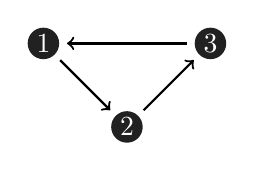
\begin{tikzpicture}[node distance=15mm,
				dot/.style={minimum size=4mm, circle, draw=none, fill=black!87, inner sep=0, outer sep=1mm, text=white}]
				
				\begin{scope}
				\node [dot] (1) {1};
				\node [dot,below right of=1] (2) {2};
				\node [dot,above right of=2] (3) {3};
				\begin{scope}[->,thick]
				\draw (1) -- (2);
				\draw (2) -- (3);
				\draw (3) -- (1);
				\end{scope}
				\end{scope}
				\end{tikzpicture}
			\column{.5\textwidth}
				\[\exists y\forall x Rxy\nvDash\forall y\exists x Rxy\]
				\centering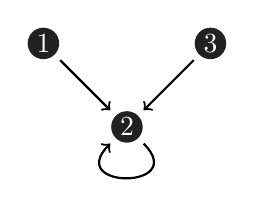
\begin{tikzpicture}[node distance=15mm,
				dot/.style={minimum size=4mm, circle, draw=none, fill=black!87, inner sep=0, outer sep=1mm, text=white}]
				
				\begin{scope}[xshift=50mm]
				\node [dot] (1) {1};
				\node [dot,below right of=1] (2) {2};
				\node [dot,above right of=2] (3) {3};
				\begin{scope}[->,thick]
				\draw (1) -- (2);
				\draw (3) -- (2);
				\draw (2) to[out=-45,in=-45-90,looseness=5] (2);
				\end{scope}
				\end{scope}
				\end{tikzpicture}
		\end{columns}
	\end{example}
}

\frame{{Is there a finite counter model?}
	\begin{exercise}[Counter Model]
		Give a counter model for
	\begin{enumerate}
		\item $\forall x\exists y Rxy\wedge\forall xyz(Rxy\wedge Ryz\to Rxz)\nvDash\exists x Rxx$
		\item $\forall x\exists y Rxy\wedge\forall xyz(Rxy\wedge Ryz\to Rxz)\nvDash\exists xy(Rxy\wedge Ryx)$
	\end{enumerate}
	\end{exercise}
\begin{prooftree}
	\AxiomC{Everybody loves somebody}
	\noLine
	\UnaryInfC{Everybody loves all persons who are loved by his loved ones}
	\alwaysSingleLine
	\UnaryInfC{There is at least a pair of persons who love each other}
\end{prooftree}
\[(\mathbb{Z},<)\]
}

\frame{{Relevance Lemma}
	\begin{lemma}[Relevance Lemma]
		Assume $\nu_1,\nu_2\colon \mathscr{V}\to A$, and for any $x\in \mathrm{Fv}(\varphi)\colon \nu_1(x)=\nu_2(x)$. Then
		\[\mathcal{A},\nu_1\vDash\varphi\iff\mathcal{A},\nu_2\vDash\varphi\]
	\end{lemma}
	\begin{itemize}
		\item If $\varphi$ is a sentence, then either $\mathcal{A}\vDash\varphi$ or $\mathcal{A}\vDash\neg\varphi$.
		\item $\mathcal{A}\vDash\varphi\implies\mathcal{A}\vDash\forall x\varphi$
		\item \textbf{Notation}: If $\mathrm{Fv}(\varphi)\subset\{x_1,\dots,x_n\}$, then we write $\mathcal{A}\vDash\varphi[a_1,\dots,a_n]$ to mean $\mathcal{A},\nu\vDash\varphi$ for some \textcolor{blue}{(equivalently any)} assignment $\nu$ s.t. $\nu(x_i)=a_i$ for $1\leq i\leq n$.
	\end{itemize}
}

\frame{{Substitution Lemma}
	\begin{columns}
		\column{.57\textwidth}
			\setlength\abovedisplayskip{0pt}
			\setlength\belowdisplayskip{0pt}
			\begin{lemma}[Substitution Lemma]
				\begin{itemize}
					\item $\nu\left(s[t/x]\right)=\nu(\nu(t)/x)(s)$
					\item If the term $t$ is substitutable for the variable $x$ in the wff $\varphi$, then
					\[\mathcal{A},\nu\vDash\varphi[t/x]\iff\mathcal{A},\nu(\nu(t)/x)\vDash\varphi\]
				\end{itemize}
			\end{lemma}
		\column{.43\textwidth}
			\begin{tcolorbox}[colback=cyan!3,colframe=back!85]
				\centering\resizebox{.63\textwidth}{!}{
					\begin{minipage}{1.35\textwidth}\hspace{-5ex}
						\begin{tikzpicture}[node distance=5cm]
						\begin{scope}[->,ultra thick]
						\node (1) {\textcolor{blue}{\huge $s$}};
						\node [below right of=1] (2) {\huge $\textcolor{blue}{ A}$};
						\node [above right of=2] (3) {\textcolor{blue}{\huge $s[t/x]$}};
						\begin{scope}[->,ultra thick]
						\draw[darkgreen, ultra thick,->,above] (1) to node{\textcolor{cyan}{\huge $[t/x]$}} (3);
						\draw[darkgreen, ultra thick,->,below of=1] (1) to node{\textcolor{red}{\huge \!\!\!\!\!\!\!\!\!\!\!\!\!\!\!\!\!\!\!\!\!\!\!\!\!\!\!\!\!\!\!\!$\overline{\nu(\overline{\nu}(t)/x)}$}} (2);
						\draw[darkgreen, ultra thick,->,below of =3] (3) to node{\textcolor{red}{\huge \qquad$\overline{\nu}$}} (2);
						\end{scope}
						\end{scope}
						\end{tikzpicture}
				\end{minipage}}
			\end{tcolorbox}
	\end{columns}
	\begin{tcolorbox}
		\[\mathscr{L}_A:=\mathscr{L}\cup\mathscr{C}_A\;\;\mbox{where}\;\;\mathscr{C}_A:=\left\{c_a\colon a\in A\right\}\]
		\[\mathcal{A},\nu\vDash\varphi[c_a/x]\iff\mathcal{A},\nu(a/x)\vDash\varphi\]
		We abbreviate $\mathcal{A},\nu\vDash\varphi[c_a/x]$ by $\mathcal{A},\nu\vDash\varphi[a]$.
		\[\textcolor{purple}{\mathcal{A},\nu\vDash\forall x\varphi\iff\;\mbox{for every}\; a\in A\colon \mathcal{A},\nu\vDash\varphi[a]}\]
	\end{tcolorbox}
}

\frame{{Equivalent Replacement}
	\begin{lemma}
		Suppose $\psi\in \mathrm{Sub}(\varphi)$, and $\varphi^*$ arises from $\varphi$ by replacing zero or more occurrences of $\psi$ by $\chi$. Then
		\[\vDash\psi\leftrightarrow\chi\implies\vDash\varphi\leftrightarrow\varphi^*\]
	\end{lemma}
}

\frame{{Alphabetic Variant}
	\begin{definition}[Alphabetic Variant]
		If $y\notin \mathrm{Fv}(\varphi)$, and $y$ is substitutable for $x$ in $\varphi$, we say that $\forall y\varphi[y/x]$ is an alphabetic variant of $\forall x\varphi$.
	\end{definition}
	\begin{theorem}
		If $\forall y\varphi[y/x]$ is an alphabetic variant of $\forall x\varphi$, then \[\vDash\forall x\varphi\leftrightarrow\forall y\varphi[y/x]\]
	\end{theorem}
	If $y\notin \mathrm{Fv}(\varphi)$, then $\varphi[y/x][x/y]=\varphi$.
	\begin{itemize}
		\item \textbf{Convention}: When we write $\varphi[t/x]$ we assume that $t$ is substitutable for $x$ in $\varphi$. --- \textit{For any formula $\varphi$ and a finite number of variables $y_1,\dots,y_n$ (occurring in $t$), we can always find a logically equivalent alphabetic variant $\varphi^*$ of $\varphi$ s.t. $y_1,\dots,y_n$ do not occur bound in $\varphi^*$.}
	\end{itemize}
}

\frame{{Equality and Equivalence}
	\begin{lemma}
		Suppose $\mathrm{Fv}(t)\cup \mathrm{Fv}(s)\subset\{x_1,\dots,x_n\}$, and $\varphi^*$ arises from the wff $\varphi$ by replacing one occurrence of $t$ in $\varphi$ by $s$. Then
		\[\vDash\forall x_1\dots x_n(t= s)\to(\varphi\leftrightarrow\varphi^*)\]
		\[\mathcal{A}\vDash t= s\implies\mathcal{A}\vDash\varphi\leftrightarrow\varphi^*\]
	\end{lemma}
	\begin{lemma}
		Suppose $\mathrm{Fv}(\psi)\cup \mathrm{Fv}(\chi)\subset\{x_1,\dots,x_n\}$, and $\varphi^*$ arises from the wff $\varphi$ by replacing one occurrence of $\psi$ in $\varphi$ by $\chi$. Then
		\[\vDash\forall x_1\dots x_n(\psi\leftrightarrow\chi)\to(\varphi\leftrightarrow\varphi^*)\]
		\[\mathcal{A}\vDash\psi\leftrightarrow\chi\implies\mathcal{A}\vDash\varphi\leftrightarrow\varphi^*\]
	\end{lemma}
}

\frame{{Remark}
	\begin{itemize}
		\item $\vDash\forall x\bigl(Px\leftrightarrow Qx\bigr)\to\bigl(\forall x Px\leftrightarrow\forall x Qx\bigr)$
		
		$\nvDash\bigl(Px\leftrightarrow Qx\bigr)\to\bigl(\forall x Px\leftrightarrow\forall x Qx\bigr)$
		\item $\mathcal{A},\nu\vDash t=s\centernot\implies\mathcal{A},\nu\vDash\varphi\leftrightarrow\varphi^*$
		\item $\mathcal{A},\nu\vDash \psi\leftrightarrow\chi\centernot\implies\mathcal{A},\nu\vDash\varphi\leftrightarrow\varphi^*$
		\[\psi=Px,\;\; \chi=Py,\;\; \varphi=\forall x Px,\;\; \varphi^*=\forall x Py\]
	\end{itemize}
}

\frame{{Valid Formulas --- Example}
	\begin{align*}
	&\forall x\varphi\to\varphi[t/x] &&\varphi[t/x]\to\exists x\varphi\\
	&\neg\forall x\varphi\leftrightarrow\exists x\neg\varphi &&\neg\exists x\varphi\leftrightarrow\forall x\neg\varphi\\
	&\forall x(\varphi\wedge\psi)\leftrightarrow\forall x\varphi\wedge\forall x\psi &&\forall x\varphi\vee\forall x\psi\to\forall x(\varphi\vee\psi)\\
	&\exists x(\varphi\vee\psi)\leftrightarrow\exists x\varphi\vee\exists x\psi &&\exists x(\varphi\wedge\psi)\to\exists x\varphi\wedge\exists x\psi\\
	&\forall x(\varphi\to\psi)\to\forall x\varphi\to\forall x\psi &&\forall x(\varphi\to\psi)\to\exists x\varphi\to\exists x\psi\\
	&\forall xy\varphi\leftrightarrow\forall yx\varphi &&\exists xy\varphi\leftrightarrow\exists yx\varphi\\
	&\exists x\forall y\varphi\to\forall y\exists x\varphi &&\\
	&\forall x(\varphi\leftrightarrow\psi)\to(\forall x\varphi\leftrightarrow\forall x\psi) &&\\
	&(\forall x\varphi\to\exists x\psi)\leftrightarrow\exists x(\varphi\to\psi)&&
	\end{align*}
}

\frame{{Valid Formulas --- Example}
	$x\notin \mathrm{Fv}(\varphi):$
	\hrule
	\begin{align*}
	&\varphi\leftrightarrow\forall x\varphi &&\varphi\leftrightarrow\exists x\varphi\\
	&\forall x(\varphi\vee\psi)\leftrightarrow\varphi\vee\forall x\psi &&\exists x(\varphi\vee\psi)\leftrightarrow\varphi\vee\exists x\psi\\
	&\forall x(\varphi\wedge\psi)\leftrightarrow\varphi\wedge\forall x\psi &&\exists x(\varphi\wedge\psi)\leftrightarrow\varphi\wedge\exists x\psi\\
	&\forall x(\varphi\to\psi)\leftrightarrow(\varphi\to\forall x\psi) &&\exists x(\varphi\to\psi)\leftrightarrow(\varphi\to\exists x\psi)\\
	&\forall x(\psi\to\varphi)\leftrightarrow(\exists x\psi\to\varphi) &&\exists x(\psi\to\varphi)\leftrightarrow(\forall x\psi\to\varphi)\\
	&&&\exists x(\varphi\to\forall x\varphi)
	\end{align*}
}

\frame{{Valid Formulas --- Example}
	\begin{align*}
	&t= t\\
	&t= s\to s= t\\
	&t= s\to s= r\to t= r\\
	&t_1= s_1\to\dots\to t_n= s_n\to f(t_1,\dots,t_n)= f(s_1,\dots,t_n)\\
	&t_1= s_1\to\dots\to t_n= s_n\to \bigl(P(t_1,\dots,t_n)\leftrightarrow P(s_1,\dots,s_n)\bigr)\\
	&t= s\to r[t/x]= r[s/x]\\
	&t= s\to\bigl(\varphi[t/x]\leftrightarrow\varphi[s/x]\bigr)
	\end{align*}
}

\frame{{Valid Formulas --- Example}
	$x\notin \mathrm{Fv}(t):$
	\hrule
	\begin{align*}
	&\exists x(x= t)\\
	&\varphi[t/x]\leftrightarrow\forall x(x= t\to\varphi)\\
	&\varphi[t/x]\leftrightarrow\exists x (x= t\wedge\varphi)
	\end{align*}
	\hrule
	\vspace{17pt}
	$\{x_1,\dots,x_n\}\cap \mathrm{Fv}(s)\cap \mathrm{Fv}(t_1)\cap\dots\cap \mathrm{Fv}(t_n)=\emptyset:$
	\hrule
	\begin{align*}
	f(t_1,\dots,t_n)&=s\\
	&\updownarrow\\
	\forall x_1\dots x_n\bigl(t_1= x_1,\dots,t_n= x_n&\to f(x_1,\dots,x_n)=s\bigr)\\
	&\updownarrow\\
	\exists x_1\dots x_n\bigl(t_1= x_1\wedge t_n= x_n&\wedge f(x_1,\dots,x_n)=s\bigr)
	\end{align*}
}

\frame{{Application --- Game}
	\begin{theorem}[Zermelo's Theorem]
		Every finite game of perfect information with no tie is determined.
	\end{theorem}
	\begin{proof}
		First, color those end nodes black that are wins for player $1$, and color the other end nodes white, being the wins for $2$. Then
		\begin{itemize}
			\item if player $1$ is to move, and at least one child is black, color it black; if all children are white, color it white.
			\item if player $2$ is to move, and at least one child is white, color it white; if all children are black, color it black.
		\end{itemize}
	\end{proof}
	\begin{proof}
		\[\exists x_1\forall y_1\dots\exists x_n\forall y_n\varphi\vee\forall x_1\exists y_1\dots\forall x_n\exists y_n\neg\varphi\]
		where $\varphi$  states that a final position is reached where player $1$ wins.
	\end{proof}
}

%%%%%%%%%%%%%%%%%%%%%%%%%%%%%%%
\subsection{Formal Systems}
%%%%%%%%%%%%%%%%%%%%%%%%%%%%%%%

\frame{{Formal Systems}
	\begin{itemize}
		\item Hilbert System
		\item Tree Method
		\item Natural Deduction
		\item Sequent Calculus
		\item Resolution
		\item \dots
	\end{itemize}
}

%-------------------------------------%
\subsubsection{Hilbert System}
%-------------------------------------%

\frame{{Hilbert System $=$ Axiom $+$ Inference Rule}\vspace{-1ex}
				\begin{alertblock}{Axiom Schema}
					\begin{enumerate}
						\item $\varphi\to\psi\to\varphi$
						\item $(\varphi\to\psi\to\chi)\to(\varphi\to\psi)\to\varphi\to\chi$
						\item $(\neg\varphi\to\neg\psi)\to(\neg\varphi\to\psi)\to\varphi$
						\item \textcolor{blue}{$\forall x(\varphi\to\psi)\to\forall x\varphi\to\forall x\psi$}
						\item \textcolor{blue}{$\forall x\varphi\to\varphi[t/x]$ where $t$ is substitutable for $x$ in $\varphi$.}
						\item \textcolor{blue}{$\varphi\to\forall x\varphi$ where $x\notin \mathrm{Fv}(\varphi)$.}
						\item $x= x$
						\item $x= y\to\varphi\to\varphi'$ where $\varphi$ is atomic and $\varphi'$ is obtained from $\varphi$ by replacing $x$ in zero or more places by $y$.
						\item \textcolor{red}{$\forall x_1\dots x_n\varphi$ where $n\geq 0$ and $\varphi$ is any axiom of the preceding groups.}
					\end{enumerate}
				\end{alertblock}
				\begin{alertblock}{Inference Rule}
					\begin{prooftree}
						\AxiomC{$\varphi$\quad$\varphi\to\psi$}
						\alwaysSingleLine
						\RightLabel{\textcolor{blue}{[MP]}}
						\UnaryInfC{$\psi$}
					\end{prooftree}
				\end{alertblock}
}

\frame{{Example}
	\begin{theorem}
		\[\varphi\vdash\exists x\varphi\]
	\end{theorem}
	\begin{proof}
		\begin{enumerate}
			\item $(\forall x\, \neg\varphi \to \neg\varphi) \to \varphi \to \neg \forall x\, \neg \varphi$ \hfill Tautology
			\item $\forall x\, \neg\varphi \to \neg\varphi$ \hfill A5
			\item $\varphi\to \neg \forall x\, \neg \varphi$ \hfill 1,2 MP
			\item $\varphi$ \hfill Premise
			\item $\neg \forall x\, \neg \varphi$ \hfill 3,4 MP
			\item $\exists x\, \varphi$ \hfill Definition of $\exists$
		\end{enumerate}
	\end{proof}
}

\frame{{Meta-properties}
	\begin{itemize}
		\item $\vDash\varphi[\psi_1/p_1,\dots,\psi_n/p_n]$ where $\varphi\in\mathscr{L}^0$, $\psi_1,\dots,\psi_n\in\mathscr{L}^1$. \hfill \textcolor{blue}{tautology}
		\item $\Gamma,\varphi\vdash\psi\iff\Gamma\vdash\varphi\to\psi$\hfill \textcolor{blue}{deduction theorem}
		\item $\Gamma,\varphi\vdash\psi\wedge\neg\psi\implies\Gamma\vdash\neg\varphi$\hfill\textcolor{blue}{reductio ad absurdum}
		\item $\Gamma,\neg\varphi\vdash\psi\;\;\&\;\;\Gamma,\neg\varphi\vdash\neg\psi\implies\Gamma\vdash\varphi$ \hfill \textcolor{blue}{proof by contradiction}
		\item $\Gamma,\varphi\vdash\neg\psi\iff\Gamma,\psi\vdash\neg\varphi$\hfill\textcolor{blue}{contraposition}
		\item $t= s\vdash r[t/x]= r[s/x]$\hfill\textcolor{blue}{substitution}
		\item $t= s\vdash\varphi[t/x]\leftrightarrow\varphi[s/x]$\hfill\textcolor{blue}{substitution}
		\item $\vdash\psi\leftrightarrow\chi\implies\vdash\varphi\leftrightarrow\varphi^*$ where $\varphi^*$ arises from $\varphi$ by replacing one or more occurrences of $\psi$ in $\varphi$ by $\chi$.\hfill \textcolor{blue}{equivalent replacement}
		\item $\vdash\forall x\varphi\iff\vdash\forall y\varphi[y/x]$ \hfill \textcolor{blue}{alphabetic variant}
	\end{itemize}
}

\frame{{Meta-properties}
	\begin{itemize}
		\item $\Gamma,\varphi[t/x]\vdash\psi\implies\Gamma,\forall x\varphi\vdash\psi$\hfill \textcolor{blue}{$\forall L$}
		\item $\Gamma\vdash\varphi[t/x]\implies\Gamma\vdash\exists x\varphi$\hfill \textcolor{blue}{$\exists R$}
		\item $\Gamma\vdash\varphi[y/x]\;\;\&\;\;y\notin\mathrm{Fv}(\Gamma,\forall x\varphi)\implies\Gamma\vdash\forall x\varphi$\hfill \textcolor{blue}{$\forall R$}
		\item $\Gamma,\varphi[y/x]\vdash\psi\;\;\&\;\;y\notin \mathrm{Fv}(\Gamma,\exists x\varphi,\psi)\implies\Gamma,\exists x\varphi\vdash\psi$\hfill \textcolor{blue}{$\exists L$}
		\item $\Gamma\vdash\varphi\;\;\&\;\;a\notin\mathrm{Cst}(\Gamma)\implies\exists y\notin\mathrm{Fv}(\varphi)\colon\Gamma\vdash\forall y\varphi[y/a]$
		\item $\Gamma\vdash\varphi[a/x]\;\;\&\;\;a\notin\mathrm{Cst}(\Gamma,\forall x\varphi)\implies\Gamma\vdash\forall x\varphi$\hfill \textcolor{blue}{$\forall R$}
		\item $\Gamma,\varphi[a/x]\vdash\psi\;\;\&\;\;a\notin\mathrm{Cst}(\Gamma,\exists x\varphi,\psi)\implies\Gamma,\exists x\varphi\vdash\psi$\hfill \textcolor{blue}{$\exists L$}
	\end{itemize}
}

\frame{{Alphabetic Variant}
	\begin{theorem}[Existence of Alphabetic Variants]
		Let $\varphi$ be a formula, $t$ a term, and $x$ a variable. Then we can find a formula $\varphi^*$ which differs from $\varphi$ only in the choice of quantified variables s.t.
		\begin{enumerate}
			\item $\varphi\dedeq\varphi^*$
			\item $t$ is substitutable for $x$ in $\varphi^*$.
		\end{enumerate}
	\end{theorem}
}

\frame{{Strategy}
	\begin{enumerate}[i]
		\item $(\to)$\quad $\Gamma\vdash\varphi\to\psi\impliedby\Gamma,\varphi\vdash\psi$
		\item $(\forall)$
		\begin{enumerate}
			\item if $x\notin \mathrm{Fv}(\Gamma)$, $\Gamma\vdash\forall x\varphi\impliedby\Gamma\vdash\varphi$
			\item if $x\in \mathrm{Fv}(\Gamma)$, $\Gamma\vdash\forall x\varphi\impliedby\Gamma\vdash\forall y\varphi[y/x]\impliedby\Gamma\vdash\varphi[y/x]$ for some new $y$.
		\end{enumerate}
		\item $(\neg)$
		\begin{enumerate}
			\item $(\neg\to)$\quad
			$\Gamma\vdash\neg(\varphi\to\psi)\impliedby\Gamma\vdash\varphi\;\;\&\;\;\Gamma\vdash\neg\psi$
			\item $(\neg\neg)$\quad $\Gamma\vdash\neg\neg\varphi\impliedby\Gamma\vdash\varphi$
			\item $(\neg\forall)$\quad
			$\Gamma\vdash\neg\forall x\varphi\impliedby\Gamma\vdash\neg\varphi[t/x]$\\ Unfortunately this is not always possible. Try contraposition, reductio ad absurdum or prove by contradiction\dots
		\end{enumerate}
	\end{enumerate}
}

%----------------------------------%
\subsubsection{Tree Method}
%----------------------------------%

\frame{{Tree Method for Propositional Logic}\vspace{-2ex}
		\begin{columns}
			\column{0.2\textwidth}
				\begin{center}
					\begin{tikzpicture}[sibling distance=10em,
					every node/.style = {align=center}]
					\node{$\neg\neg\varphi$}
					child{node{$\varphi$}};
					\end{tikzpicture}
				\end{center}
			\column{0.5\textwidth}
				\begin{center}
					\begin{tikzpicture}[sibling distance=10em,
					every node/.style = {align=center}]
					\node{$\varphi\to\psi$}
					child{node{$\neg\varphi$}}
					child{node{$\psi$}};
					\end{tikzpicture}
				\end{center}
			\column{0.2\textwidth}
				\begin{center}
					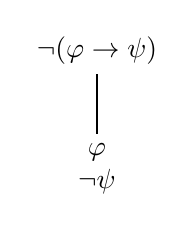
\begin{tikzpicture}[sibling distance=10em,
					every node/.style = {align=center}]
					\node{$\neg(\varphi\to\psi)$}
					child{node{$\varphi$\\$\neg\psi$}};
					\end{tikzpicture}
				\end{center}
		\end{columns}
		\vspace{7pt}
		\hrule
		\vspace{7pt}
		\begin{columns}
			\column{0.1\textwidth}
				\begin{tikzpicture}[sibling distance=10em,
				every node/.style = {align=center}]
				\node{$\varphi\wedge\psi$}
				child{node{$\varphi$\\$\psi$}};
				\end{tikzpicture}
			\column{0.35\textwidth}
				\resizebox{\textwidth}{!}{
					\begin{tikzpicture}[sibling distance=10em,
					every node/.style = {align=center}]
					\node{$\!\!\!\!\neg(\varphi\wedge\psi)$}
					child{node{$\neg\varphi$}}
					child{node{$\neg\psi$}};
					\end{tikzpicture}}
			\column{0.35\textwidth}
				\resizebox{\textwidth}{!}{
					\begin{tikzpicture}[sibling distance=10em,
					every node/.style = {align=center}]
					\node{$\varphi\vee\psi$}
					child{node{$\varphi$}}
					child{node{$\psi$}};
					\end{tikzpicture}}
			\column{0.12\textwidth}
				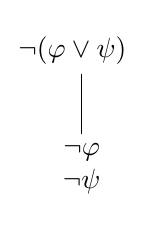
\begin{tikzpicture}[sibling distance=10em,
				every node/.style = {align=center}]
				\node{$\!\!\!\!\neg(\varphi\vee\psi)$}
				child{node{$\neg\varphi$\\$\neg\psi$}};
				\end{tikzpicture}
		\end{columns}
		\vspace{7pt}
		\hrule
		\vspace{7pt}
		\begin{columns}
			\column{0.35\textwidth}\hspace{-7pt}
				\resizebox{\textwidth}{!}{
					\begin{tikzpicture}[sibling distance=10em,
					every node/.style = {align=center}]
					\node{$\varphi\leftrightarrow\psi$}
					child{node{$\varphi$\\$\psi$}}
					child{node{$\neg\varphi$\\$\neg\psi$}};
					\end{tikzpicture}}
			\column{0.35\textwidth}\hspace{-7pt}
				\resizebox{\textwidth}{!}{
					\begin{tikzpicture}[sibling distance=10em,
					every node/.style = {align=center}]
					\node{$\neg(\varphi\leftrightarrow\psi)$}
					child{node{$\varphi$\\$\neg\psi$}}
					child{node{$\neg\varphi$\\$\psi$}};
					\end{tikzpicture}}
		\end{columns}
	\[\textcolor{red}{\checkmark}\]
}

\frame{{Tree Method for Predicate Logic \textcolor{red}{I}}
	\textcolor{red}{Ground Tree:}
	\begin{columns}
		\column{0.5\textwidth}
			\begin{center}
				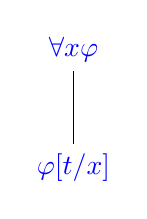
\begin{tikzpicture}[sibling distance=10em,
				every node/.style = {align=center}]
				\node{\textcolor{blue}{$\forall x\varphi$}}
				child{node{\textcolor{blue}{$\varphi[t/x]$}}};
				\end{tikzpicture}
			\end{center}
			where $t$ is a ground term.
		\column{0.5\textwidth}
			\begin{center}
				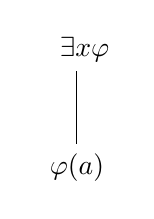
\begin{tikzpicture}[sibling distance=10em,
				every node/.style = {align=center}]
				\node{\;\;\;$\exists x\varphi\;\textcolor{red}{\checkmark}$}
				child{node{$\varphi(a)$}};
				\end{tikzpicture}
			\end{center}
			where $a$ is a new constant.
	\end{columns}
	\hrule
	\vspace{7pt}
	\begin{columns}
		\column{0.5\textwidth}
			\begin{center}
				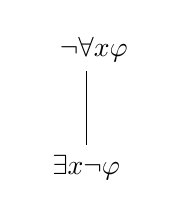
\begin{tikzpicture}[sibling distance=10em,
				every node/.style = {align=center}]
				\node{\;\;\;$\neg\forall x\varphi\;\textcolor{red}{\checkmark}$}
				child{node{$\exists x\neg\varphi$}};
				\end{tikzpicture}
			\end{center}
		\column{0.5\textwidth}
			\begin{center}
				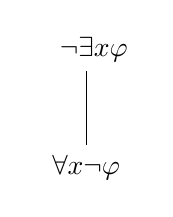
\begin{tikzpicture}[sibling distance=10em,
				every node/.style = {align=center}]
				\node{\;\;\;$\neg\exists x\varphi\;\textcolor{red}{\checkmark}$}
				child{node{$\forall x\neg\varphi$}};
				\end{tikzpicture}
			\end{center}
	\end{columns}
}

\frame{{Tree Method for Predicate Logic \textcolor{red}{II}}
	\textcolor{red}{Tree Method with Unification:}
	\begin{columns}
		\column{0.5\textwidth}
			\begin{center}
				\begin{tikzpicture}[sibling distance=10em,
				every node/.style = {align=center}]
				\node{\;\;\;$\forall x\varphi$\;\textcolor{red}{\checkmark}}
				child{node{$\varphi[x_i/x]$}};
				\end{tikzpicture}
			\end{center}
			where $x_i$ is a new variable.
		\column{0.5\textwidth}
			\begin{center}
				\begin{tikzpicture}[sibling distance=10em,
				every node/.style = {align=center}]
				\node{\;\;\;$\exists x\varphi$\;\textcolor{red}{\checkmark}}
				child{node{$\varphi[f(x_1,\dots,x_m)/x]$}};
				\end{tikzpicture}
			\end{center}
			where $f$ is a new function and $\{x_1,\dots,x_m\}=\mathrm{Fv}(\exists x\varphi)$.
	\end{columns}
	\hrule
	\vspace{7pt}
	\begin{columns}
		\column{0.5\textwidth}
			\begin{center}
				\begin{tikzpicture}[sibling distance=10em,
				every node/.style = {align=center}]
				\node{\;\;\;$\neg\forall x\varphi\;\textcolor{red}{\checkmark}$}
				child{node{$\exists x\neg\varphi$}};
				\end{tikzpicture}
			\end{center}
		\column{0.5\textwidth}
			\begin{center}
				\begin{tikzpicture}[sibling distance=10em,
				every node/.style = {align=center}]
				\node{\;\;\;$\neg\exists x\varphi\;\textcolor{red}{\checkmark}$}
				child{node{$\forall x\neg\varphi$}};
				\end{tikzpicture}
			\end{center}
	\end{columns}
}

\frame{{Tree Method with Unification}
	\begin{itemize}
		\item when expanding a universally quantified formula, do not choose a specific term but a rigid variable as a placeholder.
		\item choose the term only when it is clear it allows closing a branch.
	\end{itemize}
	\begin{center}
		\textcolor{blue}{rigid variable = same value in the whole tree}
	\end{center}
	\begin{itemize}
		\item variables can assigned to closed terms, like $x_1=a$.
		\item can also be assigned to unclosed terms, like $x_1=f(x_2)$.
	\end{itemize}
	\begin{itemize}
		\item make literals one the opposite of the other.
		\item using terms as unspecified as possible --- Given literals $A$ and $\neg B$ on the same branch, take the \textcolor{blue}{most general unifier} of $A$ and $B$.
	\end{itemize}
}

\frame{{Unifier}
\begin{tcolorbox}
\begin{itemize}
\item A substitution $\sigma$ is a \emph{unifier} for a set $\Gamma$ of formulas if for every $\varphi,\psi\in\Gamma\colon\varphi\sigma=\psi\sigma$.
\item A unifier $\sigma$ is a \emph{most general unifier} for $\Gamma$ if for each unifier $\theta$ there exists a substitution $\uplambda$ s.t. $\theta=\sigma\uplambda$.
\end{itemize}
\end{tcolorbox}
\[\sigma:=\{t_1/x_1,\dots,t_m/x_m\}\qquad \uplambda:=\{s_1/y_1,\dots,s_n/y_n\}\]
\[\sigma\uplambda=\big\{t_1\uplambda/x_1,\dots,t_m\uplambda/x_m,\; s_1/y_1,\dots,s_n/y_n\big\}\setminus\big\{s_i/y_i\colon y_i\in\{x_1,\dots,x_m\}\big\}\]
\begin{itemize}
	\item $(\varphi\sigma)\uplambda=\varphi(\sigma\uplambda)$ and $(t\sigma)\uplambda=t(\sigma\uplambda)$
	\item $(\sigma\uplambda)\theta=\sigma(\uplambda\theta)$
\end{itemize}
}

\frame{{Tree Method for Predicate Logic}
		\begin{columns}
			\column{0.5\textwidth}
				\begin{center}
					\begin{tikzpicture}[sibling distance=10em,
					every node/.style = {align=center}]
					\node{$\varphi(x)$\\$x= y$}
					child{node{$\varphi(y)$}};
					\end{tikzpicture}
				\end{center}
			\column{0.5\textwidth}
				\begin{center}
					\begin{tikzpicture}[sibling distance=10em,
					every node/.style = {align=center}]
					\node{$\varphi(x)$\\$y= x$}
					child{node{$\varphi(y)$}};
					\end{tikzpicture}
				\end{center}
		\end{columns}
		\vspace{5pt}
		where $\varphi(y)$ arises from the wff $\varphi(x)$ by replacing one or more occurrences of $x$ by $y$.
}

\frame{{Tactics}
\begin{itemize}
	\item Try to apply ``non-branching'' rules first, in order to reduce the number of branches.
	\item Try to close off branches as quickly as possible.
	\item Deal with negated quantifiers first.
	\item Instantiate existentials before universals.
\end{itemize}
}

\frame{{Example --- Ground Tree}
	\centering\fbox{$\big\{\forall x\neg P(x),\exists x(P(x)\vee P(f(x)))\big\}$ is unsatisfiable.}
	\begin{center}
		\begin{tikzpicture}[sibling distance=10em,
		every node/.style = {align=center}]
		\node{$\forall x\neg P(x)$\\$\quad\exists x(P(x)\vee P(f(x)))\;\textcolor{red}{\checkmark}$}
		child{node{$\quad P(a)\vee P(f(a))\;\textcolor{red}{\checkmark}$}
			child{node{$P(a)$}
				child{node{$\neg P(a)$\\$\textcolor{red}{\times}$}}}
			child{node{$P(f(a))$}
				child{node{$\neg P(f(a))$\\$\textcolor{red}{\times}$}}}};
		\end{tikzpicture}
	\end{center}
}

\frame{{Example --- Tree Method with Unification}
	\centering\fbox{$\big\{\forall xP(x),\neg Q(f(a)),\forall x(\neg P(f(x))\vee Q(x))\big\}$ is unsatisfiable.}
	\begin{center}
		\begin{tikzpicture}[sibling distance=10em,
		every node/.style = {align=center}]
		\node{$\quad\forall x P(x)\;\textcolor{red}{\checkmark}$\\$\neg Q(f(a))$\\$\quad\forall x(\neg P(f(x))\vee Q(x))\;\textcolor{red}{\checkmark}$}
		child{node{$P(x_1)$}
			child{node{$\quad\neg P(f(x_2))\vee Q(x_2)\;\textcolor{red}{\checkmark}$}
				child{node{$\neg P(f(x_2))$\\ {\footnotesize$x_1=f(x_2)$}\\$\textcolor{red}{\times}$}}
				child{node{$Q(x_2)$\\ {\footnotesize $x_2=f(a)$}\\$\textcolor{red}{\times}$}}}};
		\end{tikzpicture}
	\end{center}
}

\frame{{Unification --- Greedy Unification (incomplete)}\vspace{-2ex}
	\begin{center}
		\begin{tikzpicture}[sibling distance=10em,
		every node/.style = {align=center}]
		\node{$\quad\neg P(a)\;\textcolor{red}{\checkmark}$\\$\quad\neg Q(c)\;\textcolor{red}{\checkmark}$\\$\quad\neg R(d)\;\textcolor{red}{\checkmark}$\\$\forall x(((R(d)\vee\neg P(b))\wedge P(x))\vee((R(d)\vee\neg Q(b))\wedge Q(x)))\;\textcolor{red}{\checkmark}$}
		child{node{\;$\quad((R(d)\vee\neg P(b))\wedge P(x_1))\vee((R(d)\vee\neg Q(b))\wedge Q(x_1))\;\textcolor{red}{\checkmark}$}
			child{node{$\!\!\!\!\!\!\!\!\!\!\!\!\!\!\!\!\!\!\!\!\!\!\!\quad(R(d)\vee\neg P(b))\wedge P(x_1)\;\textcolor{red}{\checkmark}$}
				child{node{$\;\;R(d)\vee\neg P(b)$\\
				$P(x_1)$\\
				{\footnotesize$x_1=a$}\\$\textcolor{red}{\times}$}}}
			child{node{$\qquad(R(d)\vee\neg Q(b))\wedge Q(a)\;\textcolor{red}{\checkmark}$}
				child{node{$\quad\;\;\; R(d)\vee\neg Q(b)\;\textcolor{red}{\checkmark}$\\
				$Q(a)$}
					child{node{$R(d)$\\$\textcolor{red}{\times}$}}
					child{node{$\neg Q(b)$}}}}};
		\end{tikzpicture}
	\end{center}\vspace{-2ex}
{\small Applying unification as soon as a branch can be closed by lead to incompleteness.}
}

\frame{{Unification --- Final Closure}\vspace{-2ex}
	\begin{center}
		\begin{tikzpicture}[sibling distance=10em,
		every node/.style = {align=center}]
		\node{$\quad\neg P(a)\;\textcolor{red}{\checkmark}$\\$\quad\neg Q(c)\;\textcolor{red}{\checkmark}$\\$\quad\neg R(d)\;\textcolor{red}{\checkmark}$\\$\forall x(((R(d)\vee\neg P(b))\wedge P(x))\vee((R(d)\vee\neg Q(b))\wedge Q(x)))\;\textcolor{red}{\checkmark}$}
		child{node{\;$\quad((R(d)\vee\neg P(b))\wedge P(x_1))\vee((R(d)\vee\neg Q(b))\wedge Q(x_1))\;\textcolor{red}{\checkmark}$}
			child{node{$\!\!\!\!\!\!\!\!\!\!\!\!\!\!\!\!\!\!\!\!\!\!\!\quad(R(d)\vee\neg P(b))\wedge P(x_1)\;\textcolor{red}{\checkmark}$}
				child{node{$\quad\;\;R(d)\vee\neg P(b)\;\textcolor{red}{\checkmark}$\\
				$P(x_1)$}
					child{node{$R(d)$\\$\textcolor{red}{\times}$}}
					child{node{{}\\{}\\{}\\$\!\!\!\!\!\!\!\!\!\!\!\!\!\!\!\neg P(b)$\\
					{\footnotesize$\!\!\!\!\!\!\!\!\!\!\!\!\!\!\!\textcolor{blue}{x_1=b}$}\\$\!\!\!\!\!\!\!\!\!\!\textcolor{red}{\times}$}}}}
			child{node{$\qquad(R(d)\vee\neg Q(b))\wedge Q(x_1)\;\textcolor{red}{\checkmark}$}
				child{node{$\quad\;\;\,R(d)\vee\neg Q(b)\;\textcolor{red}{\checkmark}$\\
				$Q(x_1)$}
					child{node{$\qquad\qquad R(d)$\\$\qquad\qquad \textcolor{red}{\times}$}}
					child{node{$\neg Q(b)$\\
				{\footnotesize$\textcolor{blue}{x_1=b}$}\\$\textcolor{red}{\times}$}}}}};
		\end{tikzpicture}
	\end{center}\vspace{-3ex}
{\small Unification is applied only when it closes all open branches at the same time.}
}

\frame[shrink]{{Example --- Unification vs Ground}
	\begin{columns}
		\column{0.5\textwidth}
			\centering\fbox{存在某个人,如果她不孕,则人人不孕。}\\
			\fbox{$\vdash\exists x\big(\varphi(x)\to\forall x\varphi(x)\big)$}\vspace{-2ex}
			\begin{center}
				\begin{tikzpicture}[sibling distance=10em,
				every node/.style = {align=center}]
				\node{$\quad\neg\exists x(\varphi(x)\to\forall x\varphi(x))\;\textcolor{red}{\checkmark}$}
				child{node{$\quad\forall x\neg(\varphi(x)\to\forall x\varphi(x))\;\textcolor{red}{\checkmark}$}
					child{node{$\quad\neg(\varphi(x_1)\to\forall x\varphi(x))\;\textcolor{red}{\checkmark}$}
						child{node{$\varphi(x_1)$\\$\quad\neg\forall x\varphi(x)\;\textcolor{red}{\checkmark}$}
							child{node{$\neg\varphi(a)$\\{\footnotesize $x_1=a$}\\$\textcolor{red}{\times}$}}}}};
				\end{tikzpicture}
			\end{center}
		\column{0.5\textwidth}\vspace{-10pt}
			\begin{center}
				\begin{tikzpicture}[sibling distance=10em,
				every node/.style = {align=center}]
				\node{$\forall x\neg(\varphi(x)\to\forall x\varphi(x))$}
				child{node{$\quad\neg(\varphi(a)\to\forall x\varphi(x))\;\textcolor{red}{\checkmark}$}
					child{node{$\varphi(a)$\\$\quad\neg\forall x\varphi(x)\;\textcolor{red}{\checkmark}$}
						child{node{$\neg\varphi(b)$}
							child{node{$\quad\neg(\varphi(b)\to\forall x\varphi(x))\;\textcolor{red}{\checkmark}$}
								child{node{$\varphi(b)$\\$\neg\forall x\varphi(x)$\\$\textcolor{red}{\times}$}}}}}};
				\end{tikzpicture}
			\end{center}
	\end{columns}
}

\frame{{Soundness \& Completeness}
	\setlength\abovedisplayskip{0pt}
	\begin{definition}[Deduction]
		\[\varphi_1,\dots,\varphi_n\vdash\psi\;\text{iff there exists a closed tree from}\;\{\varphi_1,\dots,\varphi_n,\neg\psi\}.\]
	\end{definition}
	\begin{theorem}[Soundness Theorem]
		If the tree closes, the set is unsatisfiable.
	\end{theorem}
	\begin{theorem}[Completeness Theorem]
		If a set is unsatisfiable, there \textcolor{red}{exists} a closed tree from it.
	\end{theorem}
	\[\varphi_1,\dots,\varphi_n\vdash\psi\iff\varphi_1,\dots,\varphi_n\vDash\psi\]
	\textbf{Remark:} If an inference with predicate wff is not valid and its counterexample is an infinite model, the tree will not find it. The tree method cannot generate every counterexample of an invalid inference in predicate logic.
}

{\setbeamercolor{normal text}{fg=fore,bg=back}\usebeamercolor[fg]{normal text}
	\frame{{Exercises --- Tree Method}
		\begin{enumerate}
			\item $\forall x(Px\to Qx)\to\exists xPx\to\exists xQx$
			\item $\exists x\forall yRxy\to\forall y\exists xRxy$
			\item $\exists x(Px\wedge Qx)\to\exists xPx\wedge\exists xQx$
			\item $\forall x\big(\varphi\vee \psi(x)\big)\to\varphi\vee\forall x\psi(x)$ where $x\notin \mathrm{Fv}(\varphi)$
			\item $\exists x\Big(\big(Px\wedge\forall y(Py\to y=x)\big)\wedge Qx\Big)\dedeq\exists x\forall y\Big(\big(Py\leftrightarrow y=x\big)\wedge Qx\Big)$
			\item $\exists x\big(Px\wedge\forall y(Py\to y=x)\big)\wedge\exists x\big(Qx\wedge\forall y(Qy\to y=x)\big)\wedge\neg\exists x(Px\wedge Qx)\to\exists xy\big(x\ne y\wedge (Px\vee Qx)\wedge(Py\vee Qy)\wedge\forall z(Pz\vee Qz\to z=x\vee z=y)\big)$
\[1+1=2\]
		\end{enumerate}
	}
}

{\setbeamercolor{normal text}{fg=fore,bg=back}\usebeamercolor[fg]{normal text}
	\frame{{Exercises --- Tree Method}%\vspace*{-5pt}
		\begin{enumerate}
			\item Nobody trusts \emph{exactly} those who have no mutual trust with anybody.
			\item If horses are animals, every head of a horse is the head of an animal.
			\item Every non-analytic, meaningful proposition is either verifiable or falsifiable. Philosophical propositions are neither analytic nor verifiable or falsifiable. Therefore, they are meaningless.
			\item No girl loves any sexist pig. Caroline is a girl who loves whoever loves her. Henry loves Caroline. Thus Henry isn't a sexist pig.
			\item \emph{The} present king of France is bald. Bald men are sexy. Hence whoever is a present King of France is sexy.
			\item \emph{Only} Russell is a great philosopher. Wittgenstein is a great philosopher who smokes. So Russell smokes.
			\item Everyone is afraid of Dracula. Dracula is afraid \emph{only} of me. Therefore, I am Dracula.
			\item Everyone loves a \emph{lover}(\emph{anyone who loves somebody}). Romeo loves Juliet. Therefore, I love you.
			\item Everyone loves a \emph{lover}(\emph{anyone who loves somebody}); hence if someone is a lover, everyone loves everyone!
		\end{enumerate}
	}
}

{\setbeamercolor{normal text}{fg=fore,bg=back}\usebeamercolor[fg]{normal text}
	\frame{{Exercises --- Tree Method}
		\begin{enumerate}
			\item I am a genius. A genius can \emph{only} be appreciated by geniuses. No genius is without some eccentricity. I sing rock. Every eccentric rock singer is appreciated by some girl. Eccentrics are conceited. Therefore, some girl is conceited.
			\item Any philosopher admires some logician. Some students admire \emph{only} politicians. No politicians are logicians. Therefore not all students are philosophers.
			\item If anyone speaks to anyone, then someone introduces them; no one introduces anyone to anyone unless they know them both; everyone speaks to Frank; therefore everyone is introduced to Frank by someone who knows him.
			\item Whoever stole the goods, knew the safe combination. Someone stole the goods, and \emph{only} Jack knew the safe combination. Hence Jack stole the goods.
			\item \emph{No one but} Lily and Lucy (\emph{who are different people}) admires Ray. All and only those who admire Ray love him. Hence \emph{exactly} two people love Ray.
		\end{enumerate}
	}
}

\frame{{Application --- \href{http://web.mat.bham.ac.uk/R.W.Kaye/minesw/}{\textcolor{fore}{Minesweeper}}}\vspace{-5pt}
	\begin{figure}
		\includegraphics[width=0.3\textwidth,angle=0,origin=c]{img/minesweeper}
	\end{figure}\vspace{-7pt}
	\begin{itemize}
		\item There are exactly $n$ mines in the game.
		\item If a cell contains the number $1$, then there is exactly one mine in the adjacent cells.\vspace{-12pt}
		\resizebox{.9\textwidth}{!}{
			\begin{minipage}{\textwidth}
				\[\forall x(\mathit{contain}(x,1)\to\exists y(\mathit{adj}(x,y)\wedge \mathit{mine}(y)\wedge\forall z(\mathit{adj}(x,z)\wedge \mathit{mine}(z)\to z=y)))\]
		\end{minipage}}
		\item \dots
	\end{itemize}
}

\frame{{Russell's Theory of Descriptions}
\begin{columns}
\column{.6\textwidth}
\begin{enumerate}
	\item \textcolor{blue}{The substitution of identicals.}
	\underline{``The morning star is the evening star.''}
	\item \textcolor{blue}{The law of the excluded middle.}
	\underline{``The present King of France is bald.''}\;\;\textcolor{red}{or}
	\underline{``The present King of France is not bald.''}
	\item \textcolor{blue}{The problem of negative existentials.}
	\underline{``The round square is round.''}
\end{enumerate}
\column{.25\textwidth}
\begin{figure}
\includegraphics[width=\textwidth]{img/triangle-centroid-median}\\\vspace{2ex}
\includegraphics[width=.8\textwidth]{img/bald.png}
\end{figure}
\end{columns}
}

\frame{{Russell's Theory of Descriptions}
\begin{align*}
\textcolor{blue}{\psi(\iota_x\varphi):}&\textcolor{blue}{=\exists! x\varphi\wedge\exists x(\varphi\wedge\psi)}\\
&\textcolor{blue}{\equiv\exists x\forall y\Big(\big(\varphi(y)\leftrightarrow y=x\big)\wedge\psi(x)\Big)}
\end{align*}
\textcolor{red}{The} round square does not exist. \textcolor{darkgreen}{$\psi(\iota_x\varphi)\vee(\neg\psi)(\iota_x\varphi)$}\;\textcolor{red}{?}
\[\exists x\forall y\Big(\big(Ry\wedge Sy\leftrightarrow y=x\big)\wedge\neg Ex\Big)\quad\textcolor{darkgreen}{(\neg\psi)(\iota_x\varphi)}\;\textcolor{red}{?}\]
\[\neg\exists x\forall y\Big(\big(Ry\wedge Sy\leftrightarrow y=x\big)\wedge Ex\Big)\quad\textcolor{darkgreen}{\neg\psi(\iota_x\varphi)}\;\textcolor{red}{?}\]
\[Ex\stackrel{\textcolor{red}{?}}{:=}\exists P\big(Px\wedge\exists y\neg Py\big)\]
\[\iota_x\varphi=\iota_x\varphi\;\;\textcolor{red}{?}\qquad \forall x\psi\to\psi(\iota_x\varphi)\;\;\textcolor{red}{?}\]
\[\textcolor{blue}{\psi(\iota_x^y\varphi):=\big(\exists!x\varphi\to\exists x(\varphi\wedge\psi)\big)\wedge\big(\neg\exists!x\varphi\to\psi[y/x]\big)}\]
\[\vdash\forall x\psi\to\psi(\iota_x^y\varphi)\]
}

\frame{{}
\begin{itemize}
	\item The logical form of a statement may differ from its grammatical form.
	\item The correct logical analysis of a word or phrase may involve an explanation not of what that word or phrase taken by itself means, but rather of what whole sentences containing the word or phrase mean.
	\item The method of contextual definition, which the theory of descriptions exemplifies, was inspired by the nineteenth-century rigorization of analysis.
\end{itemize}
Berkeley: $2^{nd}$ crisis of the Foundations of Mathematics\\
For $f(x)=x^2$,
\[\dfrac{\mathrm{d} f(x)}{\mathrm{d}x}=\dfrac{f(x+\mathrm{d}x)-f(x)}{\mathrm{d}x}=\dfrac{(x+\mathrm{d}x)^2-x^2}{\mathrm{d}x}=\dfrac{2x\mathrm{d}x+(\mathrm{d}x)^2}{\textcolor{red}{\mathrm{d}x}}=2x+\textcolor{red}{\mathrm{d}x}=2x\]
$\dfrac{\mathrm{d}}{\mathrm{d}x}$ should be explained as a whole.
\[\dfrac{\mathrm{d} f(x)}{\mathrm{d}x}=\dfrac{\mathrm{d}}{\mathrm{d}x}f(x)=\lim\limits_{\Delta x\to 0}\dfrac{f(x+\Delta x)-f(x)}{\Delta x}\]
}

\frame{{Logicism \& Logical Positivism}
\begin{itemize}
	\item Mathematics could be reduced to logic.
	\item Science could be reduced to logical compounds of statements about sense data.
	\item Only statements verifiable through observation or logical proof are meaningful.
	\item If all you have is a hammer, everything looks like a nail.
	\item The new logical resources provided by Frege and Russell had both tempted the positivists to conjecture more than they could prove and made it clear to them that proof of their conjecture was impossible.
	\item Few if any philosophical schools before the positivists had even stated their aims with sufficient clarity to make it possible to see that they were unachievable.
\end{itemize}
}

%-------------------------------------%
\subsubsection{Natural Deduction}
%-------------------------------------%

\frame{{Gentzen}
	\begin{columns}
		\column{0.4\textwidth}\vspace{-2ex}
			\begin{figure}
				\includegraphics[width=\textwidth,angle=0,origin=c]{img/gentzen}\caption{Gentzen 1909-1945}
			\end{figure}
		\column{0.61\textwidth}
			\begin{tcolorbox}
				\begin{itemize}
					\item Natural Deduction: one proposition on the right.
					\item Sequent Calculus: zero or more propositions on the right.
					\[\Gamma\vdash\Delta\iff\vdash\bigwedge\Gamma\to\bigvee\Delta\]
					\item Consistency of $\mathrm{PA}$\\
					(proof-theoretical strength of $\mathrm{PA}$)
				\end{itemize}
			\end{tcolorbox}
	\end{columns}
}

\frame{{Natural Deduction}
	\begin{columns}
		\column{0.5\textwidth}
			\begin{prooftree}
				\AxiomC{$\varphi\in\Gamma$}
				\alwaysSingleLine
				\RightLabel{\textcolor{blue}{[I]}}
				\UnaryInfC{$\Gamma\vdash\varphi$}
			\end{prooftree}
		\column{0.5\textwidth}
			\begin{prooftree}
				\AxiomC{$\Gamma\vdash\varphi\qquad \Gamma\subset\Gamma'$}
				\alwaysSingleLine
				\RightLabel{\textcolor{blue}{[M]}}
				\UnaryInfC{$\Gamma'\vdash\varphi$}
			\end{prooftree}
	\end{columns}
	\begin{columns}
	\column{.4\textwidth}
			\begin{prooftree}
				\AxiomC{$\Gamma\vdash\varphi\qquad\Gamma\vdash\psi$}
				\alwaysSingleLine
				\RightLabel{\textcolor{blue}{[$\wedge^+$]}}
				\UnaryInfC{$\Gamma\vdash\varphi\wedge\psi$}
			\end{prooftree}
	\column{.3\textwidth}
			\begin{prooftree}
				\AxiomC{$\Gamma\vdash\varphi\wedge\psi$}
				\alwaysSingleLine
				\RightLabel{\textcolor{blue}{[$\wedge^-$]}}
				\UnaryInfC{$\Gamma\vdash\varphi$}
			\end{prooftree}
	\column{.3\textwidth}
			\begin{prooftree}
				\AxiomC{$\Gamma\vdash\varphi\wedge\psi$}
				\alwaysSingleLine
				\RightLabel{\textcolor{blue}{[$\wedge^-$]}}
				\UnaryInfC{$\Gamma\vdash\psi$}
			\end{prooftree}
	\end{columns}
	\begin{columns}
		\column{0.25\textwidth}
			\begin{prooftree}
				\AxiomC{$\Gamma\vdash\varphi$}
				\alwaysSingleLine
				\RightLabel{\textcolor{blue}{[$\vee^+$]}}
				\UnaryInfC{$\Gamma\vdash\varphi\vee\psi$}
			\end{prooftree}
		\column{0.25\textwidth}
			\begin{prooftree}
				\AxiomC{$\Gamma\vdash\varphi$}
				\alwaysSingleLine
				\RightLabel{\textcolor{blue}{[$\vee^+$]}}
				\UnaryInfC{$\Gamma\vdash\psi\vee\varphi$}
			\end{prooftree}
		\column{0.57\textwidth}
			\begin{prooftree}
				\AxiomC{$\Gamma\vdash\varphi\vee\psi\quad\;\Gamma,\varphi\vdash\chi\quad\;\Gamma,\psi\vdash\chi$}
				\alwaysSingleLine
				\RightLabel{\textcolor{blue}{[$\vee^-$]}}
				\UnaryInfC{$\Gamma\vdash\chi$}
			\end{prooftree}
	\end{columns}
	\begin{columns}
		\column{0.5\textwidth}
			\begin{prooftree}
				\AxiomC{$\Gamma,\varphi\vdash\psi$}
				\alwaysSingleLine
				\RightLabel{\textcolor{blue}{[$\to^+$]}}
				\UnaryInfC{$\Gamma\vdash\varphi\to\psi$}
			\end{prooftree}
		\column{0.5\textwidth}
			\begin{prooftree}
				\AxiomC{$\Gamma\vdash\varphi\to\psi\qquad \Gamma\vdash\varphi$}
				\alwaysSingleLine
				\RightLabel{\textcolor{blue}{[$\to^-$]}}
				\UnaryInfC{$\Gamma\vdash\psi$}
			\end{prooftree}
	\end{columns}
	\begin{columns}
		\column{0.22\textwidth}
			\begin{prooftree}
				\AxiomC{$\Gamma,\varphi\vdash\bot$}
				\alwaysSingleLine
				\RightLabel{\textcolor{blue}{[$\neg^+$]}}
				\UnaryInfC{$\Gamma\vdash\neg\varphi$}
			\end{prooftree}
		\column{0.24\textwidth}
			\begin{prooftree}
				\AxiomC{$\Gamma\vdash\neg\neg\varphi$}
				\alwaysSingleLine
				\RightLabel{\textcolor{blue}{[$\neg^-$]}}
				\UnaryInfC{$\Gamma\vdash\varphi$}
			\end{prooftree}
		\column{0.34\textwidth}
			\begin{prooftree}
				\AxiomC{$\Gamma\vdash\neg\varphi\qquad\Gamma\vdash\varphi$}
				\alwaysSingleLine
				\RightLabel{\textcolor{blue}{[$\bot^+$]}}
				\UnaryInfC{$\Gamma\vdash\bot$}
			\end{prooftree}
		\column{0.22\textwidth}
			\begin{prooftree}
				\AxiomC{$\Gamma\vdash\bot$}
				\alwaysSingleLine
				\RightLabel{\textcolor{blue}{[$\bot^-$]}}
				\UnaryInfC{$\Gamma\vdash\varphi$}
			\end{prooftree}
	\end{columns}
}

\frame{{Natural Deduction}
	\begin{columns}
		\column{0.55\textwidth}
			\begin{prooftree}
				\AxiomC{$\Gamma\vdash\varphi(a)\qquad a\notin\mathrm{Cst}(\Gamma,\forall x\varphi)$}
				\alwaysSingleLine
				\RightLabel{\textcolor{blue}{[$\forall^+$]}}
				\UnaryInfC{$\Gamma\vdash\forall x\varphi$}
			\end{prooftree}
		\column{.45\textwidth}
			\begin{prooftree}
				\AxiomC{$\Gamma\vdash\forall x\varphi$}
				\alwaysSingleLine
				\RightLabel{\textcolor{blue}{[$\forall^-$]}}
				\UnaryInfC{$\Gamma\vdash\varphi(t)$}
			\end{prooftree}
	\end{columns}
	\begin{columns}
	\column{.25\textwidth}
			\begin{prooftree}
				\AxiomC{$\Gamma\vdash\varphi(t)$}
				\alwaysSingleLine
				\RightLabel{\textcolor{blue}{[$\exists^+$]}}
				\UnaryInfC{$\Gamma\vdash\exists x\varphi$}
			\end{prooftree}
	\column{.75\textwidth}
			\begin{prooftree}
				\AxiomC{$\Gamma\vdash\exists x\varphi\qquad\Gamma,\varphi(a)\vdash\psi\qquad a\notin\mathrm{Cst}(\Gamma,\exists x\varphi,\psi)$}
				\alwaysSingleLine
				\RightLabel{\textcolor{blue}{[$\exists^-$]}}
				\UnaryInfC{$\Gamma\vdash\psi$}
			\end{prooftree}
	\end{columns}
	\begin{columns}
		\column{0.5\textwidth}
			\begin{prooftree}
				\AxiomC{}
				\alwaysSingleLine
				\RightLabel{\textcolor{blue}{[$=^+$]}}
				\UnaryInfC{$\Gamma\vdash t=t$}
			\end{prooftree}
		\column{0.5\textwidth}
			\begin{prooftree}
				\AxiomC{$\Gamma\vdash s=t\qquad\Gamma\vdash\varphi(s)$}
				\alwaysSingleLine
				\RightLabel{\textcolor{blue}{[$=^-$]}}
				\UnaryInfC{$\Gamma\vdash\varphi(t)$}
			\end{prooftree}
	\end{columns}
}

\frame{{Example}
	\begin{theorem}[Proof by Contradiction]
		\[\neg\varphi\to\bot\vdash\varphi\]
	\end{theorem}
	\begin{proof}
		\begin{prooftree}
			\AxiomC{}
			\alwaysSingleLine
			\RightLabel{\textcolor{blue}{[I]}}
			\UnaryInfC{$\neg\varphi\to\bot,\neg\varphi\vdash\neg\varphi\to\bot$}
			\AxiomC{}
			\RightLabel{\textcolor{blue}{[I]}}
			\UnaryInfC{$\neg\varphi\to\bot,\neg\varphi\vdash\neg\varphi$}
			\RightLabel{\textcolor{blue}{[$\to^-$]}}
			\BinaryInfC{$\neg\varphi\to\bot,\neg\varphi\vdash\bot$}
			\RightLabel{\textcolor{blue}{[$\neg^+$]}}
			\UnaryInfC{$\neg\varphi\to\bot\vdash\neg\neg\varphi$}
			\RightLabel{\textcolor{blue}{[$\neg^-$]}}
			\UnaryInfC{$\neg\varphi\to\bot\vdash\varphi$}
		\end{prooftree}
	\end{proof}
\centerline{\infer[\textcolor{blue}{[\neg^-]}]{\varphi}{\infer[\textcolor{blue}{[\neg^+]}^1]{\neg\neg\varphi}{\infer[\textcolor{blue}{[\to^-]}]{\bot}{\neg\varphi\to\bot &[\neg\varphi]^1}}}}
}

\frame{{Example}\centering
	\fbox{If $x\notin \mathrm{Fv}(\varphi)$, then $\vdash\forall x(\varphi\to\psi(x))\to\varphi\to\forall x\psi(x)$.}
		\begin{prooftree}
			\AxiomC{}
			\alwaysSingleLine
			\RightLabel{\textcolor{blue}{[I]}}
			\UnaryInfC{$\forall x(\varphi\to\psi(x))\vdash\forall x(\varphi\to\psi(x))$}
			\alwaysSingleLine
			\RightLabel{\textcolor{blue}{[$\forall^-$]}}
			\UnaryInfC{$\forall x(\varphi\to\psi(x))\vdash\varphi\to\psi(a)$}
			\alwaysSingleLine
			\RightLabel{\textcolor{blue}{[$\to^-$]}}
			\UnaryInfC{$\forall x(\varphi\to\psi(x)),\varphi\vdash\psi(a)$}
			\alwaysSingleLine
			\RightLabel{\textcolor{blue}{[$\forall^+$]}}
			\UnaryInfC{$\forall x(\varphi\to\psi(x)),\varphi\vdash\forall x\psi(x)$}
			\alwaysSingleLine
			\RightLabel{\textcolor{blue}{[$\to^+$]}}
			\UnaryInfC{$\forall x(\varphi\to\psi(x))\vdash\varphi\to\forall x\psi(x)$}
			\alwaysSingleLine
			\RightLabel{\textcolor{blue}{[$\to^+$]}}
			\UnaryInfC{$\vdash\forall x(\varphi\to\psi(x))\to\varphi\to\forall x\psi(x)$}
		\end{prooftree}
\centerline{\infer[\textcolor{blue}{[\to^+]}^2]{\forall x(\varphi\to\psi(x))\to\varphi\to\forall x\psi(x)}{\infer[\textcolor{blue}{[\to^+]}^1]{\varphi\to\forall x\psi(x)}{\infer[\textcolor{blue}{[\forall^+]}]{\forall x\psi(x)}{\infer[\textcolor{blue}{[\to^-]}]{\psi(a)}{\infer[\textcolor{blue}{[\forall^-]}]{\varphi\to\psi(a)}{[\forall x(\varphi\to\psi(x))]^2}&[\varphi]^1}}}}}
}

\frame{{Natural Deduction --- another version}
\begin{columns}
\column{0.3\textwidth}\centering
\infer[\textcolor{blue}{[\wedge^+]}]{\varphi\wedge\psi}{\varphi &\psi}
\column{0.3\textwidth}\centering
\infer[\textcolor{blue}{[\wedge^-]}]{\varphi}{\varphi\wedge\psi}
\column{0.3\textwidth}\centering
\infer[\textcolor{blue}{[\wedge^-]}]{\psi}{\varphi\wedge\psi}
\end{columns}
\vspace{2pt}
\hrulefill
\vspace{6pt}
\begin{columns}
\column{0.3\textwidth}\centering
\infer[\textcolor{blue}{[\vee^+]}]{\varphi\vee\psi}{\varphi}
\column{0.3\textwidth}\centering
\infer[\textcolor{blue}{[\vee^+]}]{\varphi\vee\psi}{\psi}
\column{0.4\textwidth}\centering
\infer[\textcolor{blue}{[\vee^-]}^n]{\chi}{\varphi\vee \psi & \infer*{\chi}{[\varphi]^n} & \infer*{\chi}{[\psi]^n}}
\end{columns}
\vspace{6pt}
\hrulefill
\vspace{6pt}
\begin{columns}
\column{0.3\textwidth}\centering
\infer[\textcolor{blue}{[\to^+]}^n]{\varphi\to\psi}{\infer*{\psi}{[\varphi]^n}}
\column{0.3\textwidth}\centering
\infer[\textcolor{blue}{[\to^-]}]{\psi}{\varphi\to\psi & \varphi}
\end{columns}
\vspace{6pt}
\hrulefill
\vspace{6pt}
\begin{columns}
\column{0.25\textwidth}\centering
\infer[\textcolor{blue}{[\neg^+]}^n]{\neg\varphi}{\infer*{\bot}{[\varphi]^n}}
\column{0.25\textwidth}\centering
\infer[\textcolor{blue}{[\neg^-]}]{\varphi}{\neg\neg\varphi}
\column{0.25\textwidth}\centering
\infer[\textcolor{blue}{[\bot^+]}]{\bot}{\neg\varphi & \varphi}
\column{0.25\textwidth}\centering
\infer[\textcolor{blue}{[\bot^-]}]{\varphi}{\bot}
\end{columns}
}

\frame{{Natural Deduction --- another version}
\begin{columns}
\column{0.3\textwidth}\centering
\infer[\textcolor{blue}{[\forall^+]}]{\forall x\varphi}{\varphi(a)}
\column{0.3\textwidth}\centering
\infer[\textcolor{blue}{[\forall^-]}]{\varphi(t)}{\forall x\varphi}
\end{columns}
where $a\notin\mathrm{Cst}(\forall x\varphi)$, and $a$ is not in any assumption which is undischarged in the derivation ending with $\varphi(a)$.\\
\hrulefill
\vspace{5pt}
\begin{columns}
\column{0.3\textwidth}\centering
\infer[\textcolor{blue}{[\exists^+]}]{\exists x\varphi}{\varphi(t)}
\column{0.3\textwidth}\centering
\infer[\textcolor{blue}{[\exists^-]}^n]{\psi}{\exists x\varphi & \infer*{\psi}{\big[\varphi(a)\big]^n}}
\end{columns}
where $a\notin\mathrm{Cst}(\exists x\varphi,\psi)$, and $a$ is not in any assumption which is undischarged in the derivations ending with $\exists x\varphi,\psi$ except in $\varphi(a)$.\\
\hrulefill
\vspace{5pt}
\begin{columns}
\column{0.3\textwidth}\centering
\infer[\textcolor{blue}{[=^+]}]{t=t}{}
\column{0.3\textwidth}\centering
\infer[\textcolor{blue}{[=^-]}]{\varphi(t)}{s=t & \varphi(s)}
\end{columns}
}

%-------------------------------------%
\subsubsection{Sequent Calculus}
%-------------------------------------%

\frame{{Sequent Calculus}
	Axiom\hfill \textcolor{red}{Cut}
	\hrule
	\begin{columns}
		\column{0.5\textwidth}\vspace{5pt}
			\begin{prooftree}
				\AxiomC{}
				\alwaysSingleLine
				\RightLabel{\textcolor{blue}{[I]}}
				\UnaryInfC{$\varphi\vdash\varphi$}
			\end{prooftree}
		\column{0.5\textwidth}
			\begin{prooftree}
				\AxiomC{$\Gamma\vdash\Delta,\varphi\qquad\Sigma,\varphi\vdash\Theta$}
				\alwaysSingleLine
				\RightLabel{\textcolor{blue}{[\textcolor{red}{Cut}]}}
				\UnaryInfC{$\Gamma,\Sigma\vdash\Delta,\Theta$}
			\end{prooftree}
	\end{columns}
	\vspace{10pt}
	\hrule\vspace{10pt}
	Left structural rules\hfill Right structural rules
	\hrule
	\begin{columns}
		\column{0.5\textwidth}
			\begin{prooftree}
				\AxiomC{$\Gamma\vdash\Delta$}
				\alwaysSingleLine
				\RightLabel{\textcolor{blue}{[WL]}}
				\UnaryInfC{$\Gamma,\varphi\vdash\Delta$}
			\end{prooftree}
			\begin{prooftree}
				\AxiomC{$\Gamma,\varphi,\varphi\vdash\Delta$}
				\alwaysSingleLine
				\RightLabel{\textcolor{blue}{[CL]}}
				\UnaryInfC{$\Gamma,\varphi\vdash\Delta$}
			\end{prooftree}
			\begin{prooftree}
				\AxiomC{$\Gamma_1,\varphi,\psi,\Gamma_2\vdash\Delta$}
				\alwaysSingleLine
				\RightLabel{\textcolor{blue}{[PL]}}
				\UnaryInfC{$\Gamma_1,\psi,\varphi,\Gamma_2\vdash\Delta$}
			\end{prooftree}
		\column{0.5\textwidth}
			\begin{prooftree}
				\AxiomC{$\Gamma\vdash\Delta$}
				\alwaysSingleLine
				\RightLabel{\textcolor{blue}{[WR]}}
				\UnaryInfC{$\Gamma\vdash\varphi,\Delta$}
			\end{prooftree}
			\begin{prooftree}
				\AxiomC{$\Gamma\vdash\varphi,\varphi,\Delta$}
				\alwaysSingleLine
				\RightLabel{\textcolor{blue}{[CR]}}
				\UnaryInfC{$\Gamma\vdash\varphi,\Delta$}
			\end{prooftree}
			\begin{prooftree}
				\AxiomC{$\Gamma\vdash\Delta_1,\varphi,\psi,\Delta_2$}
				\alwaysSingleLine
				\RightLabel{\textcolor{blue}{[PR]}}
				\UnaryInfC{$\Gamma\vdash\Delta_1,\psi,\varphi,\Delta_2$}
			\end{prooftree}
	\end{columns}
}

\frame{{Sequent Calculus}
	Left logical rules:\hfill Right logical rules:
	\hrule
	\begin{columns}
		\column{0.5\textwidth}
			\begin{prooftree}
				\AxiomC{$\Gamma,\varphi\vdash\Delta$}
				\alwaysSingleLine
				\RightLabel{\textcolor{blue}{[$\wedge L_1$]}}
				\UnaryInfC{$\Gamma,\varphi\wedge\psi\vdash\Delta$}
			\end{prooftree}
			\begin{prooftree}
				\AxiomC{$\Gamma,\psi\vdash\Delta$}
				\alwaysSingleLine
				\RightLabel{\textcolor{blue}{[$\wedge L_2$]}}
				\UnaryInfC{$\Gamma,\varphi\wedge\psi\vdash\Delta$}
			\end{prooftree}
			\begin{prooftree}
				\AxiomC{$\Gamma,\varphi\vdash\Delta\qquad\Sigma,\psi\vdash\Theta$}
				\alwaysSingleLine
				\RightLabel{\textcolor{blue}{[$\vee L$]}}
				\UnaryInfC{$\Gamma,\Sigma,\varphi\vee\psi\vdash\Delta,\Theta$}
			\end{prooftree}
			\begin{prooftree}
				\AxiomC{$\Gamma\vdash\varphi,\Delta\qquad\Sigma,\psi\vdash\Theta$}
				\alwaysSingleLine
				\RightLabel{\textcolor{blue}{[$\to L$]}}
				\UnaryInfC{$\Gamma,\Sigma,\varphi\to\psi\vdash\Delta,\Theta$}
			\end{prooftree}
		\column{0.5\textwidth}
			\begin{prooftree}
				\AxiomC{$\Gamma\vdash\varphi,\Delta$}
				\alwaysSingleLine
				\RightLabel{\textcolor{blue}{[$\vee R_1$]}}
				\UnaryInfC{$\Gamma\vdash\varphi\vee\psi,\Delta$}
			\end{prooftree}
			\begin{prooftree}
				\AxiomC{$\Gamma\vdash\psi,\Delta$}
				\alwaysSingleLine
				\RightLabel{\textcolor{blue}{[$\vee R_2$]}}
				\UnaryInfC{$\Gamma\vdash\varphi\vee\psi,\Delta$}
			\end{prooftree}
			\begin{prooftree}
				\AxiomC{$\Gamma\vdash\varphi,\Delta\qquad\Sigma\vdash\psi,\Theta$}
				\alwaysSingleLine
				\RightLabel{\textcolor{blue}{[$\wedge R$]}}
				\UnaryInfC{$\Gamma,\Sigma\vdash\varphi\wedge\psi,\Delta,\Theta$}
			\end{prooftree}
			\begin{prooftree}
				\AxiomC{$\Gamma,\varphi\vdash\psi,\Delta$}
				\alwaysSingleLine
				\RightLabel{\textcolor{blue}{[$\to R$]}}
				\UnaryInfC{$\Gamma\vdash\varphi\to\psi,\Delta$}
			\end{prooftree}
	\end{columns}
}

\frame{{Sequent Calculus}
	Left logical rules:\hfill Right logical rules:
	\hrule
	\begin{columns}
	\column{0.5\textwidth}
			\begin{prooftree}
				\AxiomC{$\Gamma\vdash\varphi,\Delta$}
				\alwaysSingleLine
				\RightLabel{\textcolor{blue}{[$\neg L$]}}
				\UnaryInfC{$\Gamma,\neg\varphi\vdash\Delta$}
			\end{prooftree}
	\column{0.5\textwidth}
			\begin{prooftree}
				\AxiomC{$\Gamma,\varphi\vdash\Delta$}
				\alwaysSingleLine
				\RightLabel{\textcolor{blue}{[$\neg R$]}}
				\UnaryInfC{$\Gamma\vdash\neg\varphi,\Delta$}
			\end{prooftree}
	\end{columns}
	\begin{columns}[onlytextwidth]
		\column{0.4\textwidth}
			\begin{prooftree}
				\AxiomC{$\Gamma,\varphi(t)\vdash\Delta$}
				\alwaysSingleLine
				\RightLabel{\textcolor{blue}{[$\forall L$]}}
				\UnaryInfC{$\Gamma,\forall x\varphi\vdash\Delta$}
			\end{prooftree}
		\column{0.6\textwidth}
			\begin{prooftree}
				\AxiomC{$\Gamma\vdash\varphi(a),\Delta\qquad a\notin\mathrm{Cst}(\Gamma,\Delta,\forall x\varphi)$}
				\alwaysSingleLine
				\RightLabel{\textcolor{blue}{[$\forall R$]}}
				\UnaryInfC{$\Gamma\vdash\forall x\varphi,\Delta$}
			\end{prooftree}
	\end{columns}
	\begin{columns}[onlytextwidth]
		\column{0.6\textwidth}
			\begin{prooftree}
				\AxiomC{$\Gamma,\varphi(a)\vdash\Delta\qquad a\notin\mathrm{Cst}(\Gamma,\Delta,\exists x\varphi)$}
				\alwaysSingleLine
				\RightLabel{\textcolor{blue}{[$\exists L$]}}
				\UnaryInfC{$\Gamma,\exists x\varphi\vdash\Delta$}
			\end{prooftree}
		\column{0.4\textwidth}
			\begin{prooftree}
				\AxiomC{$\Gamma\vdash\varphi(t),\Delta$}
				\alwaysSingleLine
				\RightLabel{\textcolor{blue}{[$\exists R$]}}
				\UnaryInfC{$\Gamma\vdash\exists x\varphi,\Delta$}
			\end{prooftree}
	\end{columns}
}

\frame{{}
	\begin{columns}
		\column{0.4\textwidth}
			\begin{prooftree}
				\AxiomC{}
				\alwaysSingleLine
				\RightLabel{\textcolor{blue}{[I]}}
				\UnaryInfC{$\varphi\vdash\varphi$}
				\alwaysSingleLine
				\RightLabel{\textcolor{blue}{[$\neg R$]}}
				\UnaryInfC{$\vdash\neg\varphi,\varphi$}
				\alwaysSingleLine
				\RightLabel{\textcolor{blue}{[$\vee R_2$]}}
				\UnaryInfC{$\vdash\neg\varphi\vee\varphi,\varphi$}
				\alwaysSingleLine
				\RightLabel{\textcolor{blue}{[$PR$]}}
				\UnaryInfC{$\vdash\varphi,\varphi\vee\neg\varphi$}
				\alwaysSingleLine
				\RightLabel{\textcolor{blue}{[$\vee R_1$]}}
				\UnaryInfC{$\vdash\varphi\vee\neg\varphi,\varphi\vee\neg\varphi$}
				\alwaysSingleLine
				\RightLabel{\textcolor{blue}{[$CR$]}}
				\UnaryInfC{$\vdash\varphi\vee\neg\varphi$}
			\end{prooftree}
			\begin{prooftree}
				\AxiomC{}
				\alwaysSingleLine
				\RightLabel{\textcolor{blue}{[I]}}
				\UnaryInfC{$\varphi \vdash \varphi$}
				\RightLabel{\textcolor{blue}{[$WR$]}}
				\UnaryInfC{$ \varphi \vdash \psi, \varphi$}
				\RightLabel{\textcolor{blue}{[$\neg L$]}}
				\UnaryInfC{$\varphi, \neg \varphi \vdash \psi$}
				\AxiomC{}
				\alwaysSingleLine
				\RightLabel{\textcolor{blue}{[I]}}
				\UnaryInfC{$\psi \vdash \psi$}
				\RightLabel{\textcolor{blue}{[$WL$]}}
				\UnaryInfC{$\varphi, \psi \vdash \psi$}
				\RightLabel{\textcolor{blue}{[$\vee L$]}} \BinaryInfC{$ \varphi, \neg \varphi \vee \psi \vdash \psi $}
				\RightLabel{\textcolor{blue}{[$\to R$]}} \UnaryInfC{$ \neg \varphi \vee \psi \vdash \varphi \to \psi $}
			\end{prooftree}
			\begin{prooftree}
				\AxiomC{}
				\alwaysSingleLine
				\RightLabel{\textcolor{blue}{[I]}}
				\UnaryInfC{$\varphi(a) \vdash \varphi(a)$}
				\RightLabel{\textcolor{blue}{[$\forall L$]}}
				\UnaryInfC{$\forall x\varphi(x)\vdash \varphi(a)$}
				\RightLabel{\textcolor{blue}{[$\neg L$]}}
				\UnaryInfC{$\forall x\varphi(x),\neg \varphi(a) \vdash$}
				\RightLabel{\textcolor{blue}{[$\neg R$]}}
				\UnaryInfC{$\neg \varphi(a) \vdash \neg \forall x\varphi(x)$}
				\RightLabel{\textcolor{blue}{[$\exists L$]}}
				\UnaryInfC{$ \exists x\neg \varphi(x)\vdash \neg \forall x\varphi(x)$}
			\end{prooftree}
		\column{0.6\textwidth}
			\begin{prooftree}
				\AxiomC{}
				\alwaysSingleLine
				\RightLabel{\textcolor{blue}{[I]}}
				\UnaryInfC{$\varphi \vdash\varphi$}
				\RightLabel{\textcolor{blue}{[$\wedge L_1$]}} \UnaryInfC{$\varphi \wedge \psi \vdash \varphi$}
				\RightLabel{\textcolor{blue}{[$\neg L$]}} \UnaryInfC{$\varphi \wedge \psi, \neg \varphi \vdash $}
				\AxiomC{}
				\alwaysSingleLine
				\RightLabel{\textcolor{blue}{[I]}}
				\UnaryInfC{$ \psi \vdash \psi$}
				\RightLabel{\textcolor{blue}{[$\wedge L_2$]}} \UnaryInfC{$\varphi \wedge \psi \vdash \psi$}
				\RightLabel{\textcolor{blue}{[$\neg L$]}} \UnaryInfC{$\varphi \wedge \psi, \neg \psi \vdash $}
				\RightLabel{\textcolor{blue}{[$\vee L$]}}
				\BinaryInfC{$\varphi \wedge \psi, \neg \varphi \vee \neg \psi \vdash $}
				\RightLabel{\textcolor{blue}{[$\neg R$]}}
				\UnaryInfC{$\neg \varphi \vee \neg \psi \vdash \neg (\varphi \wedge \psi)$}
			\end{prooftree}
			\begin{prooftree}
				\AxiomC{}
				\alwaysSingleLine
				\RightLabel{\textcolor{blue}{[I]}}
				\UnaryInfC{$\varphi(a,b)\vdash\varphi(a,b)$}
				\alwaysSingleLine
				\RightLabel{\textcolor{blue}{[$\forall L$]}}
				\UnaryInfC{$\forall x\varphi(x,b)\vdash\varphi(a,b)$}
				\alwaysSingleLine
				\RightLabel{\textcolor{blue}{[$\exists R$]}}
				\UnaryInfC{$\forall x\varphi(x,b)\vdash\exists y\varphi(a,y)$}
				\alwaysSingleLine
				\RightLabel{\textcolor{blue}{[$\exists L$]}}
				\UnaryInfC{$\exists y\forall x\varphi(x,y)\vdash\exists y\varphi(a,y)$}
				\alwaysSingleLine
				\RightLabel{\textcolor{blue}{[$\forall R$]}}
				\UnaryInfC{$\exists y\forall x\varphi(x,y)\vdash\forall x\exists y\varphi(x,y)$}
			\end{prooftree}
	\end{columns}
}

\frame{{Natural Deduction --- constant vs variable}
			\begin{prooftree}
				\AxiomC{$\Gamma\vdash\varphi(a)\qquad a\notin\mathrm{Cst}(\Gamma,\forall x\varphi)$}
				\alwaysSingleLine
				\RightLabel{\textcolor{blue}{[$\forall^+$]}}
				\UnaryInfC{$\Gamma\vdash\forall x\varphi$}
			\end{prooftree}
			\begin{prooftree}
				\AxiomC{$\Gamma\vdash\varphi[y/x]\qquad y\notin \mathrm{Fv}(\Gamma,\forall x\varphi)$}
				\alwaysSingleLine
				\RightLabel{\textcolor{red}{[$\forall^+$]}}
				\UnaryInfC{$\Gamma\vdash\forall x\varphi$}
			\end{prooftree}
			\begin{prooftree}
				\AxiomC{$\Gamma\vdash\exists x\varphi\qquad\Gamma,\varphi(a)\vdash\psi\qquad a\notin\mathrm{Cst}(\Gamma,\exists x\varphi,\psi)$}
				\alwaysSingleLine
				\RightLabel{\textcolor{blue}{[$\exists^-$]}}
				\UnaryInfC{$\Gamma\vdash\psi$}
			\end{prooftree}
			\begin{prooftree}
				\AxiomC{$\Gamma\vdash\exists x\varphi\qquad\Gamma,\varphi[y/x]\vdash\psi\qquad y\notin \mathrm{Fv}(\Gamma,\exists x\varphi,\psi)$}
				\alwaysSingleLine
				\RightLabel{\textcolor{red}{[$\exists^-$]}}
				\UnaryInfC{$\Gamma\vdash\psi$}
			\end{prooftree}
}

\frame{{Natural Deduction {\small --- another version ---} constant vs variable}
\begin{columns}
\column{0.3\textwidth}\centering
\infer[\textcolor{blue}{[\forall^+]}]{\forall x\varphi}{\varphi(a)}
\column{0.3\textwidth}\centering
\infer[\textcolor{red}{[\forall^+]}]{\forall x\varphi}{\varphi[y/x]}
\end{columns}
where $a\notin\mathrm{Cst}(\forall x\varphi)$, and $a$ is not in any assumption which is undischarged in the derivation ending with $\varphi(a)$.\\\textcolor{red}{where $y\notin\mathrm{Fv}(\forall x\varphi)$, and $y$ is not free in any assumption which is undischarged in the derivation ending with $\varphi[y/x]$.}\\
\hrulefill
\vspace{5pt}
\begin{columns}
\column{0.3\textwidth}\centering
\infer[\textcolor{blue}{[\exists^-]}^n]{\psi}{\exists x\varphi & \infer*{\psi}{\big[\varphi(a)\big]^n}}
\column{0.3\textwidth}\centering
\infer[\textcolor{red}{[\exists^-]}^n]{\psi}{\exists x\varphi & \infer*{\psi}{\big[\varphi[y/x]\big]^n}}
\end{columns}
where $a\notin\mathrm{Cst}(\exists x\varphi,\psi)$, and $a$ is not in any assumption which is undischarged in the derivations ending with $\exists x\varphi,\psi$ except in $\varphi(a)$.\\
\textcolor{red}{where $y\notin\mathrm{Fv}(\exists x\varphi,\psi)$, and $y$ is not free in any assumption which is undischarged in the derivations ending with $\exists x\varphi,\psi$ except in $\varphi[y/x]$.}
}

\frame{{Sequent Calculus --- constant vs variable}
			\begin{prooftree}
				\AxiomC{$\Gamma\vdash\varphi(a),\Delta\qquad a\notin\mathrm{Cst}(\Gamma,\Delta,\forall x\varphi)$}
				\alwaysSingleLine
				\RightLabel{\textcolor{blue}{[$\forall R$]}}
				\UnaryInfC{$\Gamma\vdash\forall x\varphi,\Delta$}
			\end{prooftree}
			\begin{prooftree}
				\AxiomC{$\Gamma\vdash\varphi[y/x],\Delta\qquad y\notin \mathrm{Fv}(\Gamma,\Delta,\forall x\varphi)$}
				\alwaysSingleLine
				\RightLabel{\textcolor{red}{[$\forall R$]}}
				\UnaryInfC{$\Gamma\vdash\forall x\varphi,\Delta$}
			\end{prooftree}
			\begin{prooftree}
				\AxiomC{$\Gamma,\varphi(a)\vdash\Delta\qquad a\notin\mathrm{Cst}(\Gamma,\Delta,\exists x\varphi)$}
				\alwaysSingleLine
				\RightLabel{\textcolor{blue}{[$\exists L$]}}
				\UnaryInfC{$\Gamma,\exists x\varphi\vdash\Delta$}
			\end{prooftree}
			\begin{prooftree}
				\AxiomC{$\Gamma,\varphi[y/x]\vdash\Delta\qquad y\notin \mathrm{Fv}(\Gamma,\Delta,\exists x\varphi)$}
				\alwaysSingleLine
				\RightLabel{\textcolor{red}{[$\exists L$]}}
				\UnaryInfC{$\Gamma,\exists x\varphi\vdash\Delta$}
			\end{prooftree}
}

\frame{{Cut-Elimination Theorem}\vspace{-1ex}
	\begin{theorem}[Cut-Elimination Theorem --- Gentzen1934]
		If $\Gamma\vdash\Delta$ is provable, then it is
		provable without use of the \textcolor{red}{Cut} Rule.
	\end{theorem}
	\setlength\belowdisplayskip{0pt}
	\begin{corollary}[The Subformula Property]
		If $\Gamma\vdash\Delta$ is provable, then it has a deduction all of whose formulas are subformulas of $\Gamma$ and $\Delta$.
	\end{corollary}
	\begin{corollary}[Consistency]
		A contradiction, i.e. the empty sequent $\emptyset\vdash\emptyset$, is not deducible.
	\end{corollary}
	\begin{corollary}[Conservation]
		Predicate logic is conservative over propositional logic.
	\end{corollary}
	\begin{theorem}[Cut-free Completeness Theorem]
		Let  $\Pi$ be a set of sentences. If $\Pi$ logically implies $\Gamma\vdash\Delta$, then there is a finite subset $\Sigma\subset\Pi$ s.t. $\Sigma,\Gamma\vdash\Delta$ has a cut-free proof.
	\end{theorem}
}

%----------------------------%
\subsection{Definability \& Isomorphism}
%----------------------------%

\frame{{Definability}
\setlength\abovedisplayskip{0pt}
\setlength\belowdisplayskip{0pt}
\begin{tcolorbox}[colback=cyan!3,colframe=back!85]
	\begin{center}
		\textcolor{red}{什么是“可定义”?}
	\end{center}
\end{tcolorbox}
\begin{block}{Berry Paradox}
	The smallest positive integer not definable in fewer than twelve words.
\end{block}
\begin{definition}[Definability]
\begin{itemize}
	\item $X\subset A^n$ is $Y$-definable \emph{($X\in\mathrm{Def}(\mathcal{A},Y)$)} over $\mathcal{A}$ if there is a wff $\varphi$ and $b_1,\dots,b_m\in Y^m$ s.t.
	\[X=\big\{(a_1,\dots,a_n)\colon \mathcal{A}\vDash\varphi[a_1,\dots,a_n,b_1,\dots,b_m]\big\}\]
	\item $X$ is definable in $\mathcal{A}$ if it is $\emptyset$-definable in $\mathcal{A}$.
\end{itemize}
\end{definition}
\begin{quote}
	A definition is acceptable only on condition that it implies no contradiction.\hfill --- {\sl Poincar\'e}
\end{quote}
}

\frame{{Representability}
	\begin{tcolorbox}[colback=cyan!3,colframe=back!85]
		\begin{center}
			\textcolor{red}{什么是“可表示”?}
		\end{center}
	\end{tcolorbox}
	\begin{definition}[Representable Functions]
		A $n$-ary function $f\colon\mathbb{N}^n\to\mathbb{N}$ is representable in the theory $\mathbb{T}$ iff there is a wff $\varphi(x_1,\dots,x_n,y)$ s.t. for all $a_1,\dots,a_n$,
		\setlength\belowdisplayskip{0pt}
		\[\mathbb{T}\vdash\forall y\Big(\varphi(\underline{a_1},\dots,\underline{a_n},y)\leftrightarrow y=\underline{f(a_1,\dots,a_n)}\Big)\]
	\end{definition}
	\begin{definition}[Representable Relations]
		A $n$-ary relation $R\subset\mathbb{N}^n$ is representable in the theory $\mathbb{T}$ iff there is a wff $\varphi$ s.t. for all $a_1,\dots,a_n$,
		\setlength\abovedisplayskip{0pt}
		\setlength\belowdisplayskip{0pt}
		\begin{align*}
		&( a_1,\dots,a_n)\in R\implies \mathbb{T}\vdash\varphi[a_1,\dots,a_n]\\
		&( a_1,\dots,a_n)\notin R\implies \mathbb{T}\vdash\neg\varphi[a_1,\dots,a_n]
		\end{align*}
	\end{definition}
	\centering\fbox{A function/relation is representable in Robinson $Q$ iff it is computable.}
}

\frame{{Example}
	\begin{itemize}
		\item The interval $[0,\infty)$ is definable in $\mathcal{R}=(\mathbb{R},0,1,+,\cdot)$, where the language is $\mathscr{L}=\{0,1,+,\cdot\}$.
		\[\mathcal{R}\vDash\exists y(x= y\cdot y)[a]\iff a\geq 0\]
		\item The ordering relation $<$ is definable in $\mathcal{N}=(\mathbb{N},0,S,+,\cdot)$, where the language is $\mathscr{L}=\{0,S,+,\cdot\}$.
		\[\exists z\bigl(x+S(z)= y\bigr)\]
		\item The set of primes is definable in $\mathcal{N}$ by the formula
		\[\exists y\bigl(x= S(0)+S(y)\bigr)\wedge\forall yz\bigl(x= y\cdot z\to y= S(0)\vee z= S(0)\bigr)\]
		\item $\mathbb{N}$ is definable in $(\mathbb{Z},+,\cdot)$ by
		\[\exists y_1y_2y_3y_4\Big(x=y_1^2+y_2^2+y_3^2+y_4^2\Big)\tag{\text{Lagrange four-square theorem}}\]
		\item Exponentiation $\big\{(m,n,p)\colon p=m^n\big\}$ is definable in $\mathcal{N}$. (use the Chinese remainder theorem)
	\end{itemize}
}

\frame{{Homomorphism \& Isomorphism}
	\setlength\abovedisplayskip{0pt}
	\setlength\belowdisplayskip{0pt}
	\begin{definition}[Homomorphism]
		A homomorphism $h$ of $\mathcal{A}$ into $\mathcal{B}$ is a function $h\colon A\to B$ s.t.
		\begin{itemize}
			\item For each $n$-place predicate symbol $P$ and each $n$-tuple $( a_1,\dots,a_n)\in A^n$,
			\[( a_1,\dots,a_n)\in P^{\mathcal{A}}\iff( h(a_1),\dots,h(a_n))\in P^{\mathcal{B}}\]
			\item For each $n$-place function symbol $f$ and each $n$-tuple $( a_1,\dots,a_n)\in A^n$,
			\[h\colon f^{\mathcal{A}}(a_1,\dots,a_n)\mapsto f^{\mathcal{B}}\bigl(h(a_1),\dots,h(a_n)\bigr)\]
			In the case of a constant symbol $c$ this becomes $h\colon c^{\mathcal{A}}\mapsto c^{\mathcal{B}}$.
		\end{itemize}
	\end{definition}
	\begin{itemize}
		\item An isomorphism \textcolor{orange}{(monomorphism/epimorphism)} is a bijective \textcolor{orange}{(injective/surjective)} homomorphism. $\mathcal{A}\cong\mathcal{B}$
		\item An automorphism \textcolor{orange}{(endomorphism)} is an isomorphism \textcolor{orange}{(homomorphism)} from $\mathcal{A}$ to itself.
		\item A structure $\mathcal{A}$ is rigid if it has no automorphisms other than $1_A$.
	\end{itemize}
}

\frame{{Homomorphism Theorem}
	\begin{theorem}[Homomorphism Theorem]
		Let $h$ be a homomorphism of $\mathcal{A}$ into $\mathcal{B}$, and $\nu\colon \mathscr{V}\to A$.
		\begin{enumerate}
			\item For any term $t$, $h\bigl(\overline{\nu}(t)\bigr)=\overline{h\circ\nu}(t)$
			\item For any \textcolor{blue}{open} formula $\varphi$ \textcolor{blue}{not containing $=$}, $\mathcal{A},\nu\vDash\varphi\iff\mathcal{B},h\circ\nu\vDash\varphi$
			\item If $h\colon A\rightarrowtail B$, we may delete the restriction ``not containing $=$''.
			\item If $h\colon A\twoheadrightarrow B$, we may delete the restriction ``open''.
		\end{enumerate}
	\end{theorem}
	\begin{definition}[Elementary Equivalence]
		\[\mathcal{A}\equiv\mathcal{B} \text{ if for any sentence}\;\varphi\colon \mathcal{A}\vDash\varphi\iff\mathcal{B}\vDash\varphi\]
	\end{definition}
	\[\mathcal{A}\cong\mathcal{B}\implies\mathcal{A}\equiv\mathcal{B}\]
}

\frame{{}
\begin{theorem}
$\mathcal{A}\equiv\mathcal{B}\;\;\&\;\;|A|<\infty\implies\mathcal{A}\cong\mathcal{B}$
\end{theorem}
\begin{proof}
Suppose $|A|=n$. Then $|B|=n$.

There are only finitely many functions $f_1,\dots,f_m\colon A\to B$. Assume none of $f\colon A\to B$ is an isomorphism. For each $f_i, 1\leq i\leq m$, there is a formula $\varphi_i$ s.t. $\mathcal{A}\vDash\varphi_i(a_1,\dots,a_n)$ but $\mathcal{B}\nvDash\varphi_i(f_i(a_1),\dots,f_i(a_n))$. Then we have
\[\mathcal{A}\vDash\bigwedge\limits_{i=1}^m\varphi_i(a_1,\dots,a_n)\;\;\;\&\;\;\;\mathcal{A}\vDash\exists x_1\dots x_n\bigwedge\limits_{i=1}^m\varphi_i(x_1,\dots,x_n)\]
Since $\mathcal{A}\equiv\mathcal{B}$, then $\mathcal{B}\vDash\exists x_1\dots x_n\bigwedge\limits_{i=1}^m\varphi_i(x_1,\dots,x_n)$, and $\mathcal{B}\vDash\bigwedge\limits_{i=1}^m\varphi_i(b_1,\dots,b_n)$ for some $b_1,\dots,b_n\in B$.\\
Let $f_j\colon a_i\mapsto b_i$. But $\mathcal{B}\nvDash\varphi_j(b_1,\dots,b_n)$.
\end{proof}
}

\frame{{Substructure}
	\begin{definition}[Substructure]
		$\mathcal{A}$ is called a substructure of $\mathcal{B}$ ($\mathcal{A}\subset\mathcal{B}$) iff
		\begin{itemize}
			\item $ A\subset B$
			\item
			\begin{enumerate}
				\item $P^{\mathcal{A}}=P^{\mathcal{B}}\cap A^n$ for any $n$-ary predicate symbol $P$.
				\item $f^{\mathcal{A}}=f^{\mathcal{B}}{\restriction_{A^n}}$ for any $n$-ary function symbol $f$.
			\end{enumerate}
		\end{itemize}
	\end{definition}
	\begin{tcolorbox}
	Suppose $\mathcal{A}\subset\mathcal{B}$. Then
		\begin{itemize}
			\item for any term $t(x_1,\dots,x_n)$, and any $a_1,\dots,a_n\in A$,
			\[t^{\mathcal{A}}[a_1,\dots,a_n]=t^{\mathcal{B}}[a_1,\dots,a_n]\]
			\item for any open formula $\varphi(x_1,\dots,x_n)$, and any $a_1,\dots,a_n\in A$,
			\[\mathcal{A}\vDash\varphi[a_1,\dots,a_n]\iff\mathcal{B}\vDash\varphi[a_1,\dots,a_n]\]
		\end{itemize} 
	\end{tcolorbox}
}

\frame{{Example}
	\begin{itemize}
		\item 
		$\mathscr{L}=\{0,1,+,\cdot\}, \mathcal{N}=\left(\mathbb{N},0,1,+,\cdot\right), \mathcal{R}=\left(\mathbb{R},0,1,+,\cdot\right)$
		\[\mathcal{N}\subset\mathcal{R}\]
		\item $\mathscr{L}=\{<\}, \mathcal{A}=\left(\mathbb{N},<\right), \mathcal{B}=\left(\left\{2n\colon  n\in\mathbb{N}\right\},<\right)$
		\[h\colon n\mapsto 2n, \quad h\colon\mathcal{A}\cong\mathcal{B},\quad\text{but}\quad\mathcal{A}\not\subset\mathcal{B}\]
		\item $\mathscr{L}=\{0,+\}$
		\begin{align*}
		&\mathcal{A}=\big(\mathbb{N},0^{\mathcal{A}},+^{\mathcal{A}}\big), &\text{where}\quad&0^{\mathcal{A}}=0, &&+^{\mathcal{A}}(a,b)=a+b\\
		&\mathcal{B}=\big(\left\{2^n\colon n\in\mathbb{N}\right\}, 0^{\mathcal{B}}, +^{\mathcal{B}}\big), &\text{where}\quad&0^{\mathcal{B}}=1, &&+^{\mathcal{B}}(a,b)=a\cdot b
		\end{align*}
		\[h\colon n\mapsto 2^n,\quad h\colon\mathcal{A}\cong\mathcal{B}\quad\text{but}\quad\mathcal{A}\not\subset\mathcal{B}.\]
	\end{itemize}
}

\frame{{Example}
	\begin{columns}
		\column{0.3\textwidth}
			\begin{figure}
				\includegraphics[width=\textwidth,angle=0,origin=c]{img/isomorphism-a}
			\end{figure}
		\column{0.5\textwidth}
			\begin{figure}
				\includegraphics[width=\textwidth,angle=0,origin=c]{img/isomorphism-b}
			\end{figure}
			\[\href{http://people.cs.uchicago.edu/~laci/update.html}{\text{quasipolynomial}}\;\;2^{\mathcal{O}\left((\log n)^c\right)}\]
		\column{0.2\textwidth}
			\begin{align*}
			a&\mapsto 1\\
			b&\mapsto 6\\
			c&\mapsto 8\\
			d&\mapsto 3\\
			g&\mapsto 5\\
			h&\mapsto 2\\
			i&\mapsto 4\\
			j&\mapsto 7
			\end{align*}
	\end{columns}
}

\frame{{\href{https://mathoverflow.net/questions/53122/mathematical-urban-legends}{A Story}}
	\begin{figure}
	\includegraphics[width=\textwidth]{img/joke-isomorphic}
	\end{figure}
}

\frame{{Automorphism \& Undefinability}
	\begin{corollary}
		Let $h$ be an automorphism $h\colon A\to A$, and $R\subset A^n$ definable in $\mathcal{A}$. Then for any $a_1,\dots,a_n\in  A$,
		\[( a_1,\dots,a_n)\in R\iff( h(a_1),\dots,h(a_n))\in R\]
	\end{corollary}
	\textbf{Remark:} This corollary is sometimes useful in showing that a given relation is not definable.
	\begin{example}[The set $\mathbb{N}$ is not definable in $(\mathbb{R},<)$ where $\mathscr{L}=\{<\}$.]
		$h\colon a\mapsto a^3$ is an automorphism of $\mathbb{R}$.\\
		It maps points outside of $\mathbb{N}$ into $\mathbb{N}$.
	\end{example}
	\begin{center}
		\fbox{$\mathbb{N}$ is not definable in $(\mathbb{R},0,1,+,\cdot,<)$}\\
		Natural numbers are not definable over the theory of real-closed fields.
	\end{center}
}

\frame{{Example}
	\setlength\abovedisplayskip{0pt}
	\setlength\belowdisplayskip{0pt}
\begin{example}
	The structure $\mathcal{A}:=\big(\{a,b,c\},\{(a,b),(a,c)\}\big)$\\
	where the language is $\mathscr{L}=\{E\}$.
	\[\textcolor{red}{b\;\bullet\bm{\leftarrow}\stackrel{a}{\bullet}\bm{\to}\bullet\;c}\]
	\begin{itemize}
		\item $\{b,c\}$ is definable in $\mathcal{A}$:\quad $\exists y E(y,x)$
		\item $\{b\}$ is not definable in $\mathcal{A}$.
	\end{itemize}
\end{example}
\begin{example}
Consider the vector space $\mathcal{E}:=(E,+,f_r)_{r\in\mathbb{R}}$, where $E$ is the universe, $f_r$ is the scalar multiplication by $r$.
\begin{itemize}
	\item $U:=\{\bm{x}\in E\colon |\bm{x}|=1\}$ is not definable in $\mathcal{E}$.
	\item $h\colon\bm{x}\mapsto 2\bm{x}$ is an automorphism but it does not preserve $U$.
\end{itemize}
\end{example}
}

\frame{{Ehrenfeucht-Fra\"iss\'e Game (EF Game)}
\emph{Spoiler} and \emph{Duplicator}, played on two structures $\mathcal{A}$ and $\mathcal{B}$.

Each run of the game has $n$ moves. In each move,

\begin{itemize}
	\item \emph{\textcolor{blue}{Spoiler}} picks an element from $\mathcal{A}$ or from $\mathcal{B}$.
	\item \emph{\textcolor{blue}{Duplicator}} picks an element from $\mathcal{B}$ or from $\mathcal{A}$.
\end{itemize}
\begin{itemize}
	\item \emph{Duplicator} wins the run if $(a_i,b_i)_{i=1}^n$ is a partial isomorphism from $\mathcal{A}$ to $\mathcal{B}$.
	\item \emph{Spoler} wins the run otherwise.
\end{itemize}
\begin{itemize}
	\item \textcolor{blue}{$\mathcal{A}\sim_n\mathcal{B}$} if \emph{Duplicator} has a winning strategy in the $n$-move game.
	\item \textcolor{blue}{$\mathcal{A}\equiv_n\mathcal{B}$} if $\mathcal{A}\vDash\varphi\iff\mathcal{B}\vDash\varphi$ for all sentences up to \emph{quantifier depth} $n$.
\end{itemize}
\begin{theorem}
\[\mathcal{A}\sim_n\mathcal{B}\iff \mathcal{A}\equiv_n\mathcal{B}\]
\end{theorem}
}

\frame{{Ehrenfeucht-Fra\"iss\'e Game (EF Game)}
\begin{columns}
\column{.5\textwidth}
	\begin{center}
		\begin{tikzpicture}
		\foreach \x[count=\x] in {0,1}{
			\node[fill,circle,inner sep=2pt] (a\x) at (0,\x){};
		}
		
		\foreach \x[count=\x] in {0,1}{
			\node[fill,circle,inner sep=2pt] (b\x) at (1,\x){};
		}
		
		\draw[thick,blue] (a1) -- (b1);
		\draw[thick,blue] (a1) -- (a2);
		\draw[thick,blue] (a2) -- (b2);
		\draw[thick,blue] (b1) -- (b2);
		\end{tikzpicture}
	\end{center}
\column{.5\textwidth}
	\begin{center}
		\begin{tikzpicture}
		\foreach \x[count=\x] in {0,1,2}{
			\node[fill,circle,inner sep=2pt] (a\x) at (0,\x){};
		}
		
		\foreach \x[count=\x] in {0,1,2}{
			\node[fill,circle,inner sep=2pt] (b\x) at (1,\x){};
		}
		
		\draw[thick,blue] (a1) -- (b1);
		\draw[thick,blue] (a1) -- (a2);
		\draw[thick,blue] (a2) -- (a3);
		\draw[thick,blue] (a3) -- (b3);
		\draw[thick,blue] (b1) -- (b2);
		\draw[thick,blue] (b2) -- (b3);
		\draw[thick,blue] (a2) -- (b2);
		\end{tikzpicture}
	\end{center}
\end{columns}

\[\mathcal{A}\sim_2\mathcal{B}\qquad \mathcal{A}\nsim_3\mathcal{B}\]
\[\mathcal{A}\vDash\varphi\qquad \mathcal{B}\vDash\neg\varphi\]
\[\forall xy\exists z(\neg Exy\to Exz\wedge Eyz)\]
}

\frame{{Isomorphic Embedding, Elementary Embedding}
	\setlength\abovedisplayskip{0pt}
	\setlength\belowdisplayskip{0pt}
\begin{definition}
\begin{itemize}
	\item \textbf{Isomorphic embedding} $f\colon\mathcal{A}\subset\mathcal{B}$ if there is $\mathcal{C}\subset\mathcal{B}$ s.t. $f\colon\mathcal{A}\cong\mathcal{C}$.
	\item \textbf{Elementary embedding} $f\colon\mathcal{A}\prec\mathcal{B}$ if for any wff $\varphi(x_1,\dots,x_n)$ and any $a_1,\dots,a_n\in A$,
	\[\mathcal{A}\vDash\varphi[a_1,\dots,a_n]\iff\mathcal{B}\vDash\varphi[f(a_1,),\dots,f(a_n)]\]
	\item \textbf{Elementary substructure} $\mathcal{A}\prec\mathcal{B}$ if $A\subset B\;\;\&\;\;1_A\colon\mathcal{A}\prec\mathcal{B}$.
\end{itemize}
\end{definition}
\begin{example}
\begin{itemize}
	\item $(\mathbb{N}\setminus\{0\},\leq)\subset(\mathbb{N},\leq)\qquad(\mathbb{N}\setminus\{0\},\leq)\cong(\mathbb{N},\leq)\qquad(\mathbb{N}\setminus\{0\},\leq)\nprec(\mathbb{N},\leq)$
\[\varphi(x):=\exists y(y\leq x\wedge\neg y=x)\qquad(\mathbb{N},\leq)\vDash\varphi[1]\qquad (\mathbb{N}\setminus\{0\},\leq)\nvDash\varphi[1]\]
	\item $(2\mathbb{Z},<)\subset (\mathbb{Z},<)\qquad(2\mathbb{Z},<)\cong(\mathbb{Z},<)\qquad(2\mathbb{Z},<)\nprec(\mathbb{Z},<)$
	\[\varphi(x,y):=\exists z(x<z<y)\qquad(\mathbb{Z},<)\vDash\varphi[0,2]\qquad(2\mathbb{Z},<)\nvDash\varphi[0,2]\]
\end{itemize}
\end{example}
\[f\colon\mathcal{A}\prec\mathcal{B}\iff \exists \mathcal{C}\big(f\colon\mathcal{A}\cong\mathcal{C}\prec \mathcal{B}\big)\iff\exists \mathcal{C}\big(\mathcal{A}\prec\mathcal{C}\cong\mathcal{B}\big)\]
}

\frame{{Isomorphic Embedding, Elementary Embedding}
\[(\mathbb{N},<)\subset(\mathbb{Z},<)\subset(\mathbb{Q},<)\]
\[(\mathbb{N},<)\nprec(\mathbb{Z},<)\nprec(\mathbb{Q},<)\]
\[(\mathbb{Q},0,1,+,\cdot)\subset(\mathbb{R},0,1,+,\cdot)\subset(\mathbb{C},0,1,+,\cdot)\]
\[(\mathbb{Q},0,1,+,\cdot)\nprec(\mathbb{R},0,1,+,\cdot)\nprec(\mathbb{C},0,1,+,\cdot)\]
\[(\mathbb{N},0,1,+,\cdot,<)\subset(\mathbb{Z},0,1,+,\cdot,<)\subset(\mathbb{Q},0,1,+,\cdot,<)\subset(\mathbb{R},0,1,+,\cdot,<)\]
\[(\mathbb{N},0,1,+,\cdot,<)\nprec(\mathbb{Z},0,1,+,\cdot,<)\nprec(\mathbb{Q},0,1,+,\cdot,<)\nprec(\mathbb{R},0,1,+,\cdot,<)\]
\[(\mathbb{Q},<)\prec(\mathbb{R},<)\]
\[(2\mathbb{Z},0,+,-,<)\subset(\mathbb{Z},0,+,-,<)\]
\[(2\mathbb{Z},0,+,-,<)\equiv(\mathbb{Z},0,+,-,<)\]
\[(2\mathbb{Z},0,+,-,<)\nprec(\mathbb{Z},0,+,-,<)\]
}

\frame{{Isomorphic Embedding, Elementary Embedding}
\begin{itemize}
	\item If $f\colon\mathcal{A}\cong\mathcal{B}$, then for any term $t(x_1,\dots,x_n)$, any wff $\varphi(x_1,\dots,x_n)$, and any $a_1,\dots,a_n\in A$,
	\[f(t^{\mathcal{A}}[a_1,\dots,a_n])=t^{\mathcal{B}}[f(a_1),\dots,f(a_n)]\]
	\[\mathcal{A}\vDash\varphi[a_1,\dots,a_n]\iff\mathcal{B}\vDash\varphi[f(a_1),\dots,f(a_n)]\]
	\item $f\colon\mathcal{A}\prec\mathcal{B}$ iff $f\colon\mathcal{A}\subset\mathcal{B}$ and for any wff $\exists x\varphi(x_1,\dots,x_n,x)$ and any $a_1,\dots,a_n\in A$,
\end{itemize}
\[\mathcal{B}\vDash\exists x\varphi[f(a_1),\dots,f(a_n),x]\implies\exists a\in A\colon\mathcal{B}\vDash\varphi[f(a_1),\dots,f(a_n),f(a)]\]
}

\frame{{Isomorphic Embedding, Elementary Embedding}
\begin{itemize}
	\item Let $\mathcal{A}$ be a $\mathscr{L}$-structure. $\mathcal{A}_A:=(\mathcal{A},a)_{a\in A}$ is a $\mathscr{L}_A$-structure by interpreting $c_a$ by $a$.\\
	\item Let $\mathcal{B}$ be a $\mathscr{L}$-structure, and $X\subset A\;\;\&\;\; f\colon X\to B$. $(\mathcal{B},f(a))_{a\in X}$ is a $\mathscr{L}_X$-structure by interpreting $c_a$ by $f(a)$.
\end{itemize}
\[\resizebox{\textwidth}{!}{$\mathrm{diag}(\mathcal{A}):=\big\{\varphi\colon \varphi\mbox{ is an atomic or negated atomic sentence of $\mathscr{L}_A$ and } \mathcal{A}_A\vDash\varphi\big\}$}\]
\begin{tcolorbox}
\begin{itemize}
	\item $f\colon\mathcal{A}\subset\mathcal{B}\iff(\mathcal{B},f(a))_{a\in A}\vDash\mathrm{diag}(\mathcal{A})$
	\item $f\colon\mathcal{A}\prec\mathcal{B}\iff (\mathcal{B},f(a))_{a\in A}\vDash\mathrm{Th}(\mathcal{A}_A)$
\end{itemize}
\end{tcolorbox}
\begin{tcolorbox}
	\[\mathcal{A}\prec\mathcal{B}\iff \mathcal{A}\subset\mathcal{B}\;\;\&\;\;\forall X\in\mathrm{Def}(\mathcal{B},A)\colon X\cap A\neq\emptyset\]
\end{tcolorbox}
\begin{tcolorbox}
Let $M\subset\mathbb{R}$. $(M,<)\prec(\mathbb{R},<)$ iff $(M,<)$ is a dense linear ordering without endpoints.
\end{tcolorbox}
}

\frame{{Logic as permutation-invariant theory}
	\begin{alertblock}{Logic as permutation-invariant theory.}
		The study of \textcolor{red}{invariants} under \textcolor{red}{all automorphisms} \textcolor{blue}{(symmetries)}.
	\end{alertblock}
	\begin{quote}
		A notion is ``logical'' if it is invariant under all possible one-one transformations of the universe of discourse onto itself.\par
		\hfill --- {\sl\href{https://www.tandfonline.com/doi/abs/10.1080/01445348608837096}{Tarski}}
	\end{quote}
	\begin{quote}\it
		Logic analyzes the meaning of the concepts common to all the sciences, and establishes the general laws governing the concepts.\par\hfill --- {\sl Tarski}
	\end{quote}
}

%---------------------------------%
\subsection{Normal Forms}
%---------------------------------%

\frame{{Normal Form}
	\begin{itemize}
		\item A \emph{literal} is an atomic formula or its negation.
		\item A formula is in negation normal form (NNF) iff it contains no other connectives than $\neg, \wedge, \vee$, and the negation sign $\neg$ appears in literals only.
		\item A clause is any formula of the form: $\varphi_1\vee\varphi_2\vee\dots\vee\varphi_n$, where $n\geq 1$ and $\varphi_1, \varphi_2,\dots,\varphi_n$ are literals.
		\item A Horn clause is a clause in which at most one literal is positive.
		\item An open formula is in conjuctive normal form (CNF) iff it is a conjuction of clause.
		\item  An open formula is in disjunctive normal form (DNF) iff it is a disjunction of one or more conjunctions of one or more literals.
		\item A CNF formula is in full conjunctive normal form (FCNF) if each of its variables appears exactly once in every clause. (similarly, full disjunctive normal form)
	\end{itemize}
}

\frame{{NNF/CNF/DNF}
	\begin{columns}
		\column{0.5\textwidth}
			\begin{table}[!htbp]\centering
				\begin{tabu}{c|c}
					\hline
					subformula & replaced by\\
					\hline
					$\varphi\leftrightarrow\psi$ & $(\neg\varphi\vee\psi)\wedge(\varphi\vee\neg\psi)$\\
					\hline
					$\varphi\to\psi$ & $\neg\varphi\vee\psi$\\
					\hline
					$\neg\neg\varphi$ &$\varphi$\\
					\hline
					$\neg(\varphi\vee\psi)$ & $\neg\varphi\wedge\neg\psi$\\
					\hline
					$\neg(\varphi\wedge\psi)$ & $\neg\varphi\vee\neg\psi$\\
					\hline
					$\neg\forall x\varphi$ & $\exists x\neg\varphi$\\
					\hline
					$\neg\exists x\varphi$ & $\forall x\neg\varphi$\\
					\hline
				\end{tabu}
			\end{table}
		\column{0.5\textwidth}
			\begin{table}[!htbp]\centering
				\begin{tabu}{c|c}
					\hline
					subformula & replaced by\\
					\hline
					$(\varphi\wedge\psi)\vee\chi$ & $(\varphi\vee\chi)\wedge(\psi\vee\chi)$\\
					\hline
					$\chi\vee(\varphi\wedge\psi)$ & $(\chi\vee\varphi)\wedge(\chi\vee\psi)$\\
					\hline
				\end{tabu}
			\end{table}
			\begin{table}[!htbp]\centering
				\begin{tabu}{c|c}
					\hline
					subformula & replaced by\\
					\hline
					$(\varphi\vee\psi)\wedge\chi$ & $(\varphi\wedge\chi)\vee(\psi\wedge\chi)$\\
					\hline
					$\chi\wedge(\varphi\vee\psi)$ & $(\chi\wedge\varphi)\vee(\chi\wedge\psi)$\\
					\hline
				\end{tabu}
			\end{table}
	\end{columns}
	\begin{itemize}
		\item Any formula can be equivalently transformed into NNF.
		\item Any open formula can be equivalently transformed into CNF/DNF.
	\end{itemize}
}

\frame{{PNF}
	\begin{itemize}
		\item A formula is in prenex normal form (PNF) iff all its quantifiers (if any) are in its prefix. (PCNF)
		\item Any formula can be equivalently transformed into PNF/PCNF.
	\end{itemize}
	\begin{table}[!htbp]\centering
		\begin{tabu}{c|cl}
			\hline
			subformula & replaced by\\
			\hline
			$\neg\forall x\varphi$ & $\exists x\neg\varphi$ &\\
			\hline
			$\neg\exists x\varphi$ & $\forall x\neg\varphi$ &\\
			\hline
			$\forall x\varphi(x)\wedge\forall x\psi(x)$ &$\forall x(\varphi(x)\wedge\psi(x))$ &\\
			\hline
			$\exists x\varphi(x)\vee\exists x\psi(x)$ &$\exists x(\varphi(x)\vee\psi(x))$ &\\
			\hline
			\textcolor{blue}{$\forall x\varphi(x)$} & \textcolor{blue}{$\forall y\varphi[y/x]$} &\qquad \textcolor{blue}{where $y\notin \mathrm{Fv}(\varphi)\cup \mathrm{Bv}(\varphi)$}\\
			\hline
			$\varphi\vee Qx \psi$ & $Qx(\varphi\vee\psi)$ &\qquad where $x\notin \mathrm{Fv}(\varphi)$\\
			\hline
			$\varphi\wedge Qx \psi$ & $Qx(\varphi\wedge\psi)$ &\qquad where $x\notin \mathrm{Fv}(\varphi)$\\
			\hline
			$\varphi\to\forall x\psi$ &$\forall x(\varphi\to\psi)$ &\qquad where $x\notin \mathrm{Fv}(\varphi)$\\
			\hline
			$\varphi\to\exists x \psi$ &$\exists x(\varphi\to\psi)$ &\qquad where $x\notin \mathrm{Fv}(\varphi)$\\
			\hline
			$\forall x\varphi\to\psi$ &$\exists x(\varphi\to\psi)$ &\qquad where $x\notin \mathrm{Fv}(\varphi)$\\
			\hline
			$\exists x\varphi\to\psi$ &$\forall x(\varphi\to\psi)$ &\qquad where $x\notin \mathrm{Fv}(\varphi)$\\
			\hline
		\end{tabu}
	\end{table}
}

\frame{{PNF \& Arithmetical Hierarchy}
	\begin{columns}\hspace{-5ex}
		\column{0.5\textwidth}
			\resizebox{1.2\textwidth}{!}{
				\begin{picture}(468,576)
				% basic hierarchy lines
				\put(70,110){\framebox(288,432)} % \hbox overfull, NOT
				\put(70,182){\line(4,-1){288}}
				\put(70,182){\line(4,1){288}}
				\put(358,182){\line(-4,-1){288}}
				\put(358,182){\line(-4,1){288}}
				\put(70,326){\line(4,-1){288}}
				\put(70,326){\line(4,1){288}}
				\put(358,326){\line(-4,-1){288}}
				\put(358,326){\line(-4,1){288}}
				
				% labeling
				\Large
				\put(210,122){\mbox{$\Delta_1^0$}}
				\put(80,140){\mbox{${\Sigma_1^0}$}}
				\put(330,140){\mbox{$\Pi_1^0$}}
				\put(50,140){\mbox{${\exists}$}}
				\put(370,140){\mbox{${\forall}$}}
				\put(205,176){\mbox{$\Delta_2^0$}}
				
				\put(80,212){\mbox{${\Sigma_2^0}$}}
				\put(330,212){\mbox{$\Pi_2^0$}}
				\put(42,212){\mbox{${\exists\forall}$}}
				\put(370,212){\mbox{${\forall\exists}$}}
				\put(205,248){\mbox{$\Delta_3^0$}}
				
				\put(80,284){\mbox{${\Sigma_3^0}$}}
				\put(330,284){\mbox{$\Pi_3^0$}}
				\put(34,284){\mbox{${\exists\forall\exists}$}}
				\put(370,284){\mbox{${\forall\exists\forall}$}}
				\put(205,320){\mbox{$\Delta_4^0$}}
				
				\put(80,356){\mbox{${\Sigma_4^0}$}}
				\put(330,356){\mbox{$\Pi_4^0$}}
				\put(26,356){\mbox{${\exists\forall\exists\forall}$}}
				\put(370,356){\mbox{${\forall\exists\forall\exists}$}}
				\put(205,392){\mbox{$\Delta_5^0$}}
				\put(210,420){\mbox{$\vdots$}}
				
				\put(150,474){\mbox{${\rm AH}={\bigcup\limits_{i=1}^{\infty}{\Sigma_i^0}}
						={\bigcup\limits_{i=1}^{\infty}{\Pi_i^0}}$}}
				
				\normalsize
				\end{picture}}
		\column{0.5\textwidth}\vspace{-9ex}
			\begin{figure}
				\includegraphics[width=\textwidth,angle=0,origin=c]{img/complexity-hierarchy}
			\end{figure}
	\end{columns}
}

\frame{{Skolem Normal Form}
	\begin{itemize}
		\item A formula is in \emph{Skolem normal form} (SNF) iff it is in PNF (PCNF) without existential quantifiers. 
		\item Skolemization: Replace $\forall x_1\dots\forall x_n\exists y\varphi$ by $\forall x_1\dots\forall x_n\varphi[f(x_1,\dots,x_n)/y]$, where $f$ is a new function symbol. If there are no universal quantifiers preceding $\exists$, replace $\exists x\varphi$ by $\varphi[c/x]$, where $c$ is a new constant. Given $\varphi$, in finitely many steps we can obtain its \emph{Skolem normal form} $\varphi^{\mathrm{SNF}}$ without existential quantifiers.
		\item Any formula can be \emph{equisatisfiably} transformed into SNF.
	\end{itemize}
	Warning: $\varphi^{\mathrm{SNF}}\vDash\varphi$ but the converse is not true in general.
	\begin{exercise}[Transform the following sentence into SNF]
	Who loves all animals, is in turn loved by someone.
	\end{exercise}
}

\frame{{Herbrand Normal Form}
	\begin{center}
		\fbox{$\varphi$ is satisfiable iff $\varphi^{\mathrm{SNF}}$ is satisfiable.}
		\[\varphi^{\mathrm{HNF}}:=\left(\neg(\neg\varphi)^{\mathrm{SNF}}\right)^{\mathrm{NNF}}\]
		\fbox{$\vDash\varphi\iff\vDash\varphi^{\mathrm{HNF}}$}
	\end{center}
	Example:
	\[(\forall x\exists y\forall z\varphi(x,y,z))^{\mathrm{SNF}}=\forall xz\varphi(x,f(x),z)\]
	\[(\forall x\exists y\forall z\varphi(x,y,z))^{\mathrm{HNF}}=\exists y\varphi(c,y,f(y))\]
}

\frame{{Herbrand Universe}
\begin{definition}[Herbrand Universe]
Given a sentence $\varphi$ in Skolem normal form,
\begin{itemize}
	\item $H_0:=\{\mbox{all constants in } \varphi\}$. If no constant in $\varphi$ then $H_0:=\{c\}$ for a new constant $c$.
	\item $H_{i+1}:=\big\{f(t_1,\dots,t_n)\colon f \mbox{ in } \varphi \mbox{ and } t_j\in H_i,\; j=1,\dots, n\big\}$
	\item $H_\varphi:=\bigcup\limits_{i\in\omega}H_i$
\end{itemize}
\end{definition}
The Herbrand universe of a language $\mathscr{L}$ is the set of all ground terms of $\mathscr{L}$. If no constant in $\mathscr{L}$, then add a new constant to $\mathscr{L}$.
}

\frame{{Herbrand Structure}
\begin{definition}[Herbrand Structure]
A Herbrand structure for $\mathscr{L}$ is $(H,I)$ s.t.
\begin{itemize}
	\item $H$ is the Herbrand universe of $\mathscr{L}$.
	\item for every ground term $t$, $I(t)=t$.
\end{itemize}
\end{definition}
\begin{theorem}
A formula $\varphi$ is satisfiable iff there is a Herbrand structure satisfying it.
\end{theorem}
\begin{proof}
Assume $\varphi$ is in Skolem normal form, and it is satisfied by some structure $(A,I)$. Then Herbrand structure $(H_\varphi,J)\vDash\varphi$, where for each ground term $t\colon J(t)=t$, and for each predicate symbol $P$, $J(P)=\big\{(t_1,\dots,t_n)\in H_\varphi\colon A,I\vDash P(t_1,\dots,t_n)\big\}$.
\end{proof}
}

\frame{{Herbrand's Theorem}
For a quantifier-free wff $\varphi(x_1,\dots,x_n)$, the Herbrand expansion over a set $D$ of ground terms is $\mathcal{E}(\varphi,D):=\big\{\varphi(t_1,\dots,t_n)\colon t_i\in D\big\}$.
\begin{definition}[Herbrand's Theorem]
A sentence $\forall\bm{x}\varphi(\bm{x})$ in Skolem normal form is unsatisfiable iff some finite subset $K\subset\mathcal{E}(\varphi,H_\varphi)$ is unsatisfiable.
\end{definition}
	\begin{theorem}[Herbrand's Theorem]
		Suppose $\varphi$ is a sentence. Then
		\[\vdash\varphi\iff\vdash\bigvee\limits_{k=1}^m\varphi'(t_{k1},\dots,t_{kn})\]
		for some $m>0$ and a finite sequence of terms $t_{ij}$ with $1\leq i\leq m$ and $1\leq j\leq n$, where $\varphi'$ is obtained from $\varphi^{\mathrm{HNF}}$ by dropping the quantifiers.
	\end{theorem}
}

\frame{{Resolution --- Example}
Given clauses $A=\varphi(f(x))\vee \psi(x)$ and $B=\neg \varphi(x)\vee\neg \varphi(y)$.
\begin{enumerate}
\item Separate their variables by standard substitutions $\{x_1/x\}$ and $\{y_1/x,y_2/y\}$.
\[A'=\big\{\varphi(f(x_1)), \psi(x_1)\big\}\quad B'=\big\{\neg \varphi(y_1), \neg \varphi(y_2)\big\}\]
\item Pick a subset $C\subset A'$ containing literals all of the same sign, and a subset $D\subset B'$ containing literals all of the opposite sign of $C$ such that $|C\cup D|$ is unifiable.
\[C=\big\{\varphi(f(x_1))\big\}\quad D=\big\{\neg \varphi(y_1), \neg \varphi(y_2)\big\}\]
\[|C\cup D|=\big\{\varphi(f(x_1)), \varphi(y_1), \varphi(y_2)\big\}\]
\item A most general unifier for $|C\cup D|$ is
\[\sigma=\big\{f(x_1)/y_1,f(x_1)/y_2\big\}\]
\item A resolvent for $A$ and $B$ is:
\[R=(A'\sigma\setminus C\sigma)\cup(B'\sigma\setminus D\sigma)=\big\{\psi(x_1)\big\}\]
\end{enumerate}
}

\frame{{Resolution}
\begin{theorem}[Soundness]
If $R$ is a resolvent of $A$ and $B$, then any model satisfying both $A$ and $B$ will also satisfy $R$.
\end{theorem}
\begin{itemize}
\item For a wff $\varphi$, $\mathcal{R}(\varphi)$ is $\varphi$ extended with all resolvents to clauses of $\varphi$.
\item The successive application of the resolution rule yields a complete proof procedure.
\end{itemize}
\begin{theorem}[Completeness]
If $\varphi$ is unsatisfiable, then $\mathcal{R}^n(\varphi)$ will contain the empty clause for some $n$.
\end{theorem}
}

%---------------------------------%
\subsection{Meta-Theorems}
%---------------------------------%

\frame{{Model \& Semantic Consequence}
\begin{columns}
\column{.4\textwidth}
	\begin{itemize}
		\item $\mathrm{Mod}(\varphi):=\left\{\mathcal{A}\colon \mathcal{A}\vDash\varphi\right\}$
		\item \textcolor{red}{$\mathrm{Mod}(\Gamma):=\bigcap\limits_{\varphi\in\Gamma}\mathrm{Mod}(\varphi)$}
		\item $\mathrm{Th}(\mathcal{A}):=\left\{\varphi\colon \mathcal{A}\vDash\varphi\right\}$
		\item \textcolor{red}{$\mathrm{Th}(\mathcal{K}):=\bigcap\limits_{\mathcal{A}\in\mathcal{K}}\mathrm{Th}(\mathcal{A})$}
		\item $\mathrm{Cn}(\Gamma):=\left\{\varphi\colon \Gamma\vDash\varphi\right\}$
	\end{itemize}
\column{.6\textwidth}
	\begin{tcolorbox}
		\begin{itemize}
			\item \textcolor{blue}{$\Gamma\subset\Gamma'\implies\mathrm{Mod}(\Gamma')\subset\mathrm{Mod}(\Gamma)$}
			\item \textcolor{blue}{$\mathcal{K}\subset\mathcal{K}'\implies\mathrm{Th}(\mathcal{K}')\subset\mathrm{Th}(\mathcal{K})$}
			\item \textcolor{blue}{$\Gamma\subset\mathrm{Th}(\mathrm{Mod}(\Gamma))$}
			\item \textcolor{blue}{$\mathcal{K}\subset\mathrm{Mod}(\mathrm{Th}(\mathcal{K}))$}
			\item $\mathrm{Mod}(\Gamma)=\mathrm{Mod}(\mathrm{Th}(\mathrm{Mod}(\Gamma)))$
			\item $\mathrm{Th}(\mathcal{K})=\mathrm{Th}(\mathrm{Mod}(\mathrm{Th}(\mathcal{K})))$
			\item $\mathrm{Cn}(\Gamma)=\mathrm{Th}(\mathrm{Mod}(\Gamma))$
			\item $\Gamma\subset\Gamma'\implies \mathrm{Cn}(\Gamma)\subset \mathrm{Cn}(\Gamma')$
			\item $\mathrm{Cn}(\mathrm{Cn}(\Gamma))=\mathrm{Cn}(\Gamma)$
		\end{itemize}
	\end{tcolorbox}
\end{columns}
}

\frame{{Galois Correspondence}
	\setlength\abovedisplayskip{0pt}
	\setlength\belowdisplayskip{0pt}
\begin{definition}[Galois Correspondence]
The function $X\mapsto X^*$ from $P(A)$ to $P(B)$ and the function $Y\mapsto Y^\dagger$ from $P(B)$ to $P(A)$ constitute a \emph{Golois correspondence} if
\begin{enumerate}
	\item $X_1\subset X_2\implies X_2^*\subset X_1^*$
	\item $Y_1\subset Y_2\implies Y_2^\dagger\subset Y_1^\dagger$
	\item $X\subset(X^*)^\dagger$
	\item $Y\subset(Y^\dagger)^*$
\end{enumerate}
\end{definition}
\begin{definition}[Polarity]
Given $R\subset A\times B$, $X\subset A$, $Y\subset B$. Let
\[X^*:=\bigcap_{x\in X}\{y\in B\colon Rxy\}\qquad Y^\dagger:=\bigcap_{y\in Y}\{x\in A\colon Rxy\}\]
We refer to the functions $X\mapsto X^*$ and $Y\mapsto Y^\dagger$ as \emph{polarities}.
\end{definition}
\begin{itemize}\small
	\item The polarities induced by a relation constitute a Galois correspondence.
	\item Every Galois correspondence arises from ploarities induced by a relation.
\end{itemize}
}

\frame{{Theory \& Axiomatization}
	\begin{itemize}
		\item A set $\Gamma$ of sentences is a \textcolor{blue}{theory} if $\Gamma=\mathrm{Cn}(\Gamma)$.
		\item A theory $\Gamma$ is \textcolor{blue}{complete} if for every sentence $\varphi$, either $\varphi\in\Gamma$ or $\neg\varphi\in\Gamma$.
		\item A theory $\Gamma$ is \textcolor{darkgreen}{finitely axiomatizable} if $\Gamma=\mathrm{Cn}(\Sigma)$ for some finite set $\Sigma$ of sentences.
		\item A theory $\Gamma$ is \textcolor{purple}{axiomatizable} if there is a decidable set $\Sigma$ of sentences s.t. $\Gamma=\mathrm{Cn}(\Sigma)$.
		\item A class $\mathcal{K}$ of structures is an \textcolor{darkgreen}{elementary class ($EC$)} if $\mathcal{K}=\mathrm{Mod}(\varphi)$ for some sentence $\varphi$.
		\item A class $\mathcal{K}$ of structures is an \textcolor{purple}{elementary class in wider sense ($EC_\Delta$)} if $\mathcal{K}=\mathrm{Mod}(\Sigma)$ for some set $\Sigma$ of sentences.
	\end{itemize}
}

\frame{{Consistency \& Satisfiability}
	\begin{itemize}
		\item $\Gamma$ is \textcolor{blue}{consistent} if $\Gamma\nvdash\bot$.
		\item $\Gamma$ is \textcolor{blue}{maximal} if for every wff $\varphi$, either $\varphi\in\Gamma$ or $\neg\varphi\in\Gamma$.
		\item $\Gamma$ is \textcolor{blue}{maximal consistent} if it is both consistent and maximal.
	\end{itemize}
	\begin{itemize}
		\item $\Gamma$ is \textcolor{blue}{satisfiable} if $\mathrm{Mod}(\Gamma)\neq\emptyset$.
		\item $\Gamma$ is \textcolor{blue}{finitely satisfiable} if every finite subset of $\Gamma$ is satisfiable.
	\end{itemize}
}

\frame{{Soundness Theorem}
	\begin{theorem}[Soundness Theorem]
		\[\Gamma\vdash\varphi\implies\Gamma\vDash\varphi\]
	\end{theorem}
	\begin{proof}
		by induction on derivation lengths.
	\end{proof}
	\centering \emph{\textcolor{blue}{Truth in a model is preserved under making deductions.}}
}

\frame{{Completeness Theorem}
		\begin{theorem}[Completeness Theorem --- G\"odel1930]
			\[\Gamma\vDash\varphi\implies\Gamma\vdash\varphi\]
		\end{theorem}
		\begin{corollary}
			Any \textcolor{red}{consistent} set of wffs is \textcolor{red}{satisfiable}.
		\end{corollary}\vspace{-5ex}
		{\huge \[\arraycolsep=0.7pt\def\arraystretch{1.7}
			\begin{array}{cccc}
			&\Gamma\vDash\varphi&\iff&\Gamma\vdash\varphi\\
			&\rotatebox[origin=C]{90}{$\iff$}&&\rotatebox[origin=C]{90}{$\iff$}\\
			&\Gamma\cup\{\neg\varphi\}\atop{\text{unsatisfiable}}&\iff&\Gamma\cup\{\neg\varphi\}\atop{\text{inconsistent}}
			\end{array}
			\]}
}

\frame{{Proof of Completeness Theorem --- step$1$}
	\begin{lemma}[Lindenbaum Lemma]
		Any consistent set $\Theta$ of sentences can be extended to a maximal consistent set $\Delta$ of sentences of the same language.
	\end{lemma}
	\begin{proof}
		Arrange all the sentences in a sequence $\langle\varphi_\xi\colon \xi<\kappa\rangle$.
		\begin{align*}
		\Theta_0&:=\Theta\\
		\Theta_{\xi+1}&:=
		\begin{cases}
		\Theta_\xi\cup\left\{\varphi_\xi\right\}&\text{if $\Theta_\xi\cup\left\{\varphi_\xi\right\}$ is consistent}\\
		\Theta_\xi\cup\left\{\neg\varphi_\xi\right\}&\text{otherwise}
		\end{cases}\\
		\Theta_\xi&:=\bigcup\limits_{\alpha<\xi}\Theta_\alpha\;\quad\qquad\text{if $\xi$ is a limit ordinal}
		\end{align*}
		$\Delta:=\bigcup\limits_{\xi<\kappa}\Theta_\xi$ is maximal consistent.
	\end{proof}
}

\frame{{Proof of Completeness Theorem --- step$2$}\vspace{-3pt}
	A set $\Delta$ is Henkin iff $\Delta$ is maximally consistent and for any formula of the form $\exists x\varphi$ there exists a constant $c$ s.t. $\exists x\varphi\to\varphi[c/x]\in\Delta$.\vspace{-3pt}
	\begin{lemma}[Closure Lemma]
		If $\Gamma$ is consistent, then there is a Henkin set $\Delta\supset\Gamma$.
	\end{lemma}\vspace{-3pt}
	\begin{proof}
		Let $\mathscr{C}$ be a set of new constants. $\mathscr{L}^+:=\mathscr{L}\cup\mathscr{C}$, $\mathscr{L}\cap\mathscr{C}=\emptyset$, $|\mathscr{C}|=|\mathscr{L}|$.\\
		Assume $|\mathscr{C}|=\kappa$, and $\mathscr{C}=\left\{c_\xi\colon \xi<\kappa\right\}$. Arrange all formulas of $\mathscr{L}^+$ with at most one free variable in a sequence $\langle\varphi_\xi\colon \xi<\kappa\rangle$. Let\vspace{-13pt}
		\begin{columns}
			\column{.55\textwidth}
				\begin{align*}
				\Gamma_0&:=\Gamma\\
				\Gamma_{\xi+1}&:=\Gamma_{\xi}\cup\left\{\exists x\varphi_\xi(x)\to\varphi_\xi[c_{\beta}/x]\right\}\\
				\Gamma_\xi&:=\bigcup\limits_{\alpha<\xi}\Gamma_\alpha\quad\text{if $\xi$ is a limit ordinal}
				\end{align*}
			\column{.45\textwidth}
				where $c_\beta$ is the first new constant not occurring in $\Gamma_\xi\cup\left\{\varphi_\xi\right\}$.
		\end{columns}
		Then $\Theta:=\bigcup\limits_{\xi<\kappa}\Gamma_\xi$ is consistent, and we can extend $\Theta$ to a maximal consistent set $\Delta\supset\Theta$ by Lindenbaum lemma.
	\end{proof}
}

\frame{{Proof of Completeness Theorem --- step$3$}
	\begin{lemma}[Term Models Lemma]
		If $\Delta$ is maximal consistent, then there is an interpretation $\mathcal{A},\nu$ s.t.
		\[\mathcal{A},\nu\vDash\varphi\iff\varphi\in\Delta\]
	\end{lemma}
	\begin{proof}
		\begin{itemize}
			\item $ A:=\left\{[t]\colon t\in\mathcal{T}\right\}$ where $\mathcal{T} $ is the set of all terms of $\mathscr{L}^+$,\\
			$[t]:=\{s\colon s\sim t\}$, $s\sim t:= s=t\in\Delta$
			\item $\left( [t_1],\dots,[t_n]\right)\in P^{\mathcal{A}}:= P\left(t_1,\dots,t_n\right)\in\Delta$
			\item $f^{\mathcal{A}}\left([t_1],\dots,[t_n]\right):=[f(t_1,\dots,t_n)]$
			\item $c^{\mathcal{A}}=[c]$
			\item $\nu(x):=[x]$
		\end{itemize}
	\end{proof}
}

\frame{{\href{http://mat.msgsu.edu.tr/~dpierce/Notes/Ultraproducts/}{\textcolor{fore}{Stone Space of Lindenbaum Algebra}}}
\begin{columns}[onlytextwidth]\hspace{-1cm}
\column{.5\textwidth}\vspace{-3.5cm}
\begin{equation*}
\xymatrix@!0@=2.3cm{
\mathrm{Str}\ar@{>>}[d]_{\mathcal{A} \mapsto \mathrm{Th}(\mathcal{A})}
&\mathrm{Sen}\ar@{<~>}[l]_{\vDash}\ar@{>>}[d]^{\varphi \mapsto [\varphi]}\\
\mathrm{S_0}\rule[-1.7ex]{0ex}{2ex}
\ar@{<~>}[ur]_{\ni}\ar@{<~>}[r]\ar@{>->}[d]_{T \mapsto T/\sim}
&\mathrm{Lin_0}\\
\mathrm{Sto}(\mathrm{Lin_0})\ar@{<~>}[ur]_{\ni}}
\end{equation*}
\column{1.1\textwidth}
\resizebox{\textwidth}{!}{
\begin{minipage}{\textwidth}\vspace{2ex}
\begin{itemize}
	\item $\mathrm{Str}$: the class of structures.
	\item $\mathrm{Sen}$: the set of sentences.
	\item $\mathrm{S_0}$: the set of complete theories.
	\item $\mathrm{Lin_0}=\mathrm{Sen}/\sim$
	\item $\mathrm{Sto}(A)$: the set of ultrafilters of $A$.
\end{itemize}
\end{minipage}}\vspace{2ex}
\resizebox{.7\textwidth}{!}{\hspace{-2.7cm}
\begin{minipage}{\textwidth}
\begin{enumerate}
	\item The closed subsets of $\mathrm{Sen}$ are precisely the theories.
	\item The closed subsets of $\mathrm{S_0}$ compose a Hausdorff topology.
	\item $\mathcal{A} \mapsto \mathrm{Th}(\mathcal{A})\colon\mathrm{Str}\to\mathrm{S_0}$ is continuous, and $[\mathcal{A}]\mapsto\mathrm{Th}(\mathcal{A})$ is a homomorphism, $\mathrm{S_0}$ is a Kolmogorov quotient $\mathrm{Str}/\equiv$.
	\item For every theory $T$, $T/\sim$ is a filter of $\mathrm{Lin_0}$.
	\item For every complete theory $T$, $T/\sim$ is an ultrafilter of $\mathrm{Lin_0}$.
	\item $T\mapsto T/\sim\colon\mathrm{S_0}\rightarrowtail\mathrm{Sto}(\mathrm{Lin_0})$ is a homomorphism.
	\item The image is dense in $\mathrm{Sto}(\mathrm{Lin_0})$.
	\item The image is a closed subspace of $\mathrm{Sto}(\mathrm{Lin_0})$.
	\item $T\mapsto T/\sim\colon\mathrm{S_0}\biject\mathrm{Sto}(\mathrm{Lin_0})$ iff the topology on $\mathrm{S_0}$ is compact.
\end{enumerate}
\end{minipage}}
\end{columns}
}

\frame{{Compactness Theorem}
	\begin{theorem}[Compactness Theorem]
		A set of wffs is satisfiable iff it is finitely satisfiable.
	\end{theorem}
	\begin{corollary}
		If $\Gamma\vDash\varphi$, then there is a finite $\Gamma_0\subset\Gamma$ s.t. $\Gamma_0\vDash\varphi$.
	\end{corollary}
	\begin{corollary}
		If a set $\Gamma$ of sentences has arbitrarily large finite models, then it has an infinite model.
	\end{corollary}
	\begin{corollary}
		There is a countable structure $\mathcal{M}\equiv\mathcal{N}$ but $\mathcal{M}\ncong\mathcal{N}$.
	\end{corollary}
}

\frame{{Ultraproduct \& \L o\'s Theorem}
	\setlength\abovedisplayskip{0pt}
	\setlength\belowdisplayskip{0pt}
	\begin{definition}[Ultraproduct]
		Suppose $\{\mathcal{A}_i\colon i\in I\}$ is a set of structures, and $U$ is an ultrafilter on $I$. Define $\mathcal{B}:=\prod\limits_{i\in I}\mathcal{A}_i\big\slash\!U$ as follows:
		\begin{itemize}
			\item $B:=\prod\limits_{i\in I}A_i\big\slash\!\!\sim \;= \Big\{[f]\colon f\in\prod\limits_{i\in I} A_i\Big\}$ where $f\sim g:=\big\{i\in I\colon f(i)=g(i)\big\}\in U$
			\item $P^{\mathcal{B}}\big([f_1],\dots,[f_n]\big):=\left\{i\in I\colon P^{\mathcal{A}_i}(f_1(i),\dots,f_n(i))\right\}\in U$
			\item $F^{\mathcal{B}}\big([f_1],\dots,[f_n]\big):=[f]$ where $f(i):=F^{\mathcal{A}_i}\big(f_1(i),\dots,f_n(i)\big)$
		\end{itemize}
	\end{definition}
	\begin{theorem}[\L o\'s Theorem]
		\[\prod\limits_{i\in I}\mathcal{A}_i\big\slash\!U\;\vDash\varphi\left([f_1],\dots,[f_n]\right)\iff\left\{i\in I\colon\mathcal{A}_i\vDash\varphi\big(f_1(i),\dots,f_n(i)\big)\right\}\in U\]
	\end{theorem}
}

\frame{{Ultrapower}
	\begin{tcolorbox}
	Let $j\colon a\mapsto[f_a]$, where $f_a(i)=a$ for $i\in I$. Then
	\[j\colon\mathcal{A}\prec\prod\limits_{i\in I}\mathcal{A}\big\slash\!U\]
	\end{tcolorbox}
	\begin{theorem}[Kiesler-Shelah]
	$\mathcal{A}\equiv\mathcal{B}$ iff for some $I$ and an ultrafilter $U$ on $I$, $\prod\limits_{i\in I}\mathcal{A}\big\slash\!U\cong\prod\limits_{i\in I}\mathcal{B}\big\slash\!U$.
	\end{theorem}
}

\frame{{Compactness Theorem}
\setlength\abovedisplayskip{0pt}
\setlength\belowdisplayskip{0pt}
	\begin{corollary}[Compactness Theorem]
		A set $\Gamma$ of wffs is satisfiable iff it is finitely satisfiable.
	\end{corollary}
	\begin{proof}
		Let $I:=\big\{\Delta\subset\Gamma\colon |\Delta|<\infty\big\}$.\\
		Then $\forall \Delta\in I\;\exists \mathcal{A}_\Delta\colon \mathcal{A}_\Delta\vDash\Delta$.\\
		Let $\hat{\varphi}:=\{\Delta\in I\colon\varphi\in\Delta\}$.\\
		Then $F:=\{\hat{\varphi}\colon\varphi\in\Gamma\}$ has the finite intersection property because
		\[\{\varphi_1,\dots,\varphi_n\}\in\hat{\varphi}_1\cap\dots\cap\hat{\varphi}_n\]
		By the ultrafilter theorem, $F$ can be extended to an ultrafilter $U$ on $I$.\\
		For $\varphi\in\Gamma$,
		\begin{align*}
		\hat{\varphi}\in U\;\;\&\;\;\hat{\varphi}\subset\{\Delta\in I\colon\mathcal{A}_\Delta\vDash\varphi\}&\implies\{\Delta\in I\colon\mathcal{A}_\Delta\vDash\varphi\}\in U\\
		&\implies\prod\limits_{\Delta\in I}\mathcal{A}_\Delta\big\slash\!U\;\vDash\varphi
		\end{align*}
	\end{proof}
}

\frame{{Compactness and Compactification}
\begin{columns}
\column{.66\textwidth}
\begin{itemize}
	\item Extreme value theorem: A continuous real-valued function on a compact space is bounded and attains its maximum and minimum values.
	\item A subset of a topological space is \emph{compact} if every open cover of it has a finite subcover.
	\item Heine-Borel Theorem: A subset of $\mathbb{R}$ is compact iff it is closed and bounded.
	\item Cantor's Intersection Theorem: A decreasing nested sequence of non-empty, closed and bounded subsets of $\mathbb{R}$ has a non-empty intersection.
	\item Bolzano-Weierstrass Theorem: Every bounded sequence of real numbers has a convergent subsequence.
\end{itemize}
\column{.32\textwidth}
\centerline{\textcolor{red}{Compactness}}\vspace*{1ex}
\centerline{finite $\implies$ infinite}
\centerline{local $\implies$ global}\vspace*{2ex}
\centerline{\textcolor{red}{Compactification}}
\[\mathbb{R}\implies\mathbb{R}\cup\{-\infty,+\infty\}\]
\begin{tikzpicture}
\draw[very thick](0,1)circle(1 and 1);
\draw[line width=1pt](-2,0) -- (2,0)node[below,midway](O){0};
\draw[red,line width=1pt](0,2) -- (1,0);
\draw[red,line width=1pt](0,2) -- (-1.5,0);
\draw[red,line width=1pt](-2,2) -- (2,2);
\draw[red,line width=1pt](0,0) -- (0,2);
\node at (0,2.2) {N};
\end{tikzpicture}
\[x\mapsto\left(\frac{x}{1+x^2},\frac{x^2}{1+x^2}\right)\]
\end{columns}
}

\frame{{Nonstandard Analysis}
	\begin{columns}
		\column{0.5\textwidth}
			\begin{theorem}
				There is a structure $\mathcal{R}^*$ s.t.
				\[\mathcal{R}\equiv\mathcal{R}^*\quad \mathcal{R}\subset\mathcal{R}^*\]
			\end{theorem}
			\begin{proof}
				\[\mathrm{Th}(\mathcal{R})\cup\left\{x>c_r\colon r\in\mathbb{R}\right\}\]
			\end{proof}
		\column{0.23\textwidth}
			\begin{figure}
				\includegraphics[width=\textwidth,angle=0,origin=c]{img/robinson}\caption{Robinson}
			\end{figure}
	\end{columns}
}

\frame{{Nonstandard Analysis}
Let $U$ be a nonprinciple ultrafilter on $\mathbb{N}$.
\[\prod\limits_{i\in\mathbb{N}}\mathcal{R}\big\slash\!U\vDash\mathrm{Th}(\mathcal{R})\]
Let $\varepsilon:=\left[(1,\frac{1}{2},\frac{1}{3},\dots)\right]\in\mathbb{R}$.\\
For any $n\in\mathbb{N}$,
\[\prod\limits_{i\in\mathbb{N}}\mathcal{R}\big\slash\!U\vDash\varepsilon<\frac{1}{n}\]
}

\frame{{}
\begin{theorem}
\begin{itemize}
	\item $\mathcal{K}$ is $EC_\Delta$ iff $\mathcal{K}$ is closed under ultraproducts and elementary equivalence.
	\item $\mathcal{K}$ is $EC$ iff both $\mathcal{K}$ and the complement of $\mathcal{K}$ are closed under ultraproducts and elementary equivalence.
\end{itemize}
\end{theorem}
}

\frame{{Applications of Compactness}
	\begin{itemize}
		\item The class of all finite structures is not $EC_\Delta$. (Model finiteness is undefinable even by a set of formulas.)
		\item The class of all infinite structures is $EC_\Delta$ but not $EC$. (Model infiniteness is definable by a set of formulas but undefinable by a single formula.)
		\item The class of graphs / groups / rings / fields / ordered fields / $n$-dimensional vector spaces / fields of characteristic $p$ is $EC$; the class of infinite groups / divisible groups / torsion-free groups / infinite rings / infinite-dimensional vector spaces / fields of characteristic $0$ is $EC_\Delta$ but not $EC$; the class of all connected graphs / finite graphs / finite groups / finite rings / finite fields / algebraically closed fields / torsion groups / finite-dimensional vector spaces / noetherian commutative rings is not $EC_\Delta$.
	\end{itemize}
}

\frame{{\small Applications of Compactness --- Ramsey in the Dining Room}
	\begin{problem}[Complete Disorder is Impossible!]
		\begin{itemize}
			\item How many people do you need to invite in a party in order to have that either at least $n$ of them are mutual strangers or at least $n$ of them are mutual acquaintances?
			\item How may we know that such number exists for any $n$?
		\end{itemize}
	\end{problem}
	\begin{columns}
		\column{0.3\textwidth}
			\begin{center}
				\begin{figure}
					\includegraphics[width=\textwidth,angle=0,origin=c]{img/pigeonhole.png}
				\end{figure}
			\end{center}
		\column{0.4\textwidth}
			\begin{center}\vspace{-7pt}
				\begin{tikzpicture}
				\node[
				regular polygon,
				regular polygon sides=5,
				minimum width=4.2cm,
				] (PG) {}
				(PG.corner 1) node (PG1) {1}
				(PG.corner 2) node (PG2) {2}
				(PG.corner 3) node (PG3) {3}
				(PG.corner 4) node (PG4) {4}
				(PG.corner 5) node (PG5) {5}
				;
				\foreach \S/\E in {2/1, 3/2, 4/3, 5/4, 1/5}{\draw[-,line width=1mm,red] (PG\S) -- (PG\E);}
				\foreach \S/\E in {3/1, 1/4, 4/2, 2/5, 5/3}{\draw[-,line width=1mm,blue] (PG\S) -- (PG\E);}
				\end{tikzpicture}
			\end{center}
		\column{.3\textwidth}
		\begin{figure}
		\includegraphics[width=\textwidth]{img/beautiful-mind.jpg}
		\end{figure}
	\end{columns}
}

\frame{{Applications of Compactness}
	\begin{theorem}[Infinite Ramsey Theorem]
		If $(V,E)$ is a graph with infinitely many vertices, then it has an infinite clique or an infinite independent set.
	\end{theorem}
	\begin{theorem}[Finite Ramsey Theorem]
		For every $m,n\geq 1$ there is an integer $R(m,n)$ s.t. any graph with at least $R(m,n)$ vertices has a clique with $m$ vertices or an independent set with $n$ vertices.
	\end{theorem}
	\vspace{-2ex}
	\[R(m,n)\leq R(m-1,n)+R(m,n-1)\]
	\[R(m,n)\leq \binom{m+n-2}{m-1}\]
}

\frame{{Ramsey Number}\vspace{-1ex}
	\hspace{-1ex}\resizebox{.68\textwidth}{!}{
		\begin{minipage}{\textwidth}
			\begin{table}\[
				\begin{tabu}{!{\vrule width1pt}c!{\vrule width1.5pt}c|c|c|c|c|c|c|c|c|c!{\vrule width1pt}}
				\Xhline{1pt}
				m,n & 1 & 2  & 3     & 4        & 5          & 6           & 7           & 8           & 9           & 10          \\
				\Xhline{1.5pt}
				1    & {\bm{1}} & 1  & 1     & 1        & 1          & 1           & 1           & 1           & 1           & 1           \\
				\hline
				2    & 1 & {\bm{2}}  & 3     & 4        & 5          & 6           & 7           & 8           & 9           & 10          \\
				\hline
				3    & 1 & 3  & {\bm{6}}     & 9        & 14         & 18          & 23          & 28          & 36          & 40-42       \\
				\hline
				4    & 1 & 4  & 9     & {\bm{18}}       & 25       & 36-41       & 49-61       & 59-84    & 73-115      & 92-149      \\
				\hline
				5    & 1 & 5  & 14    & 25     & {\bm{43-48}}    & 58-87       & 80-143      & 101-216     & 133-316  & 149-442  \\
				\hline
				6    & 1 & 6  & 18    & 36-41    & 58-87      & {\bm{102-165}}     & 115-298  & 134-495  & 183-780  & 204-1171 \\
				\hline
				7    & 1 & 7  & 23    & 49-61    & 80-143     & 115-298  & {\bm{205-540}}     & 217-1031    & 252-1713 & 292-2826 \\
				\hline
				8    & 1 & 8  & 28    & 59-84 & 101-216    & 134-495  & 217-1031    & {\bm{282-1870}}    & 329-3583 & 343-6090 \\
				\hline
				9    & 1 & 9  & 36    & 73-115   & 133-316 & 183-780  & 252-1713 & 329-3583 & {\bm{565-6588}}    & 581-12677   \\
				\hline
				10   & 1 & 10 & 40-42 & 92-149   & 149-442 & 204-1171 & 292-2826 & 343-6090 & 581-12677   & {\bm{798-23556}}   \\
				\Xhline{1pt}
				\end{tabu}\]
			\end{table}
	\end{minipage}}\vspace{-20pt}
	\begin{columns}
		\column{.5\textwidth}
		\begin{figure}
			\includegraphics[width=.45\textwidth,angle=0,origin=c]{img/ramsey1}\vspace{-2ex}\caption{Ramsey 1903-1930}
		\end{figure}
		\column{0.5\textwidth}
		\begin{figure}
			\includegraphics[width=.9\textwidth,angle=0,origin=c]{img/erdos-tao}\vspace{-2ex}\caption{Erd\H{o}s 1913-1996}
		\end{figure}
	\end{columns}
}

\frame{{Ramsey Number --- Probabilistic Method}
	\begin{theorem}		
		\[\forall k\geq 2\colon R(k,k)\geq 2^{\frac{k}{2}}\]
	\end{theorem}
	\begin{proof}
		$R(2,2)=2, R(3,3)=6$. Assume $k\geq 4$. Suppose $N<2^{\frac{k}{2}}$, and consider all random red-blue
		colorings. Let A be a set of vertices of size $k$. The probability of the event $A_R$ that the edges in $A$ are all colored red is then $2^{-\binom{k}{2}}$. Hence the probability $p_R$ for some $k$-set to be colored all red is bounded by
		\[p_R=P\left(\bigcup\limits_{|A|=k}A_R\right)\leq\sum\limits_{|A|=k}P(A_R)=\binom{N}{k}2^{-\binom{k}{2}}<\dfrac{1}{2}\]
		By symmetry, $p_B<\frac{1}{2}$. So $p_R+p_B<1$ for $N<2^{\frac{k}{2}}$.
	\end{proof}
}

\frame{{Complete Disorder is Impossible!}
	\begin{theorem}[Hales-Jewett Theorem]
		For every $k,n\in\mathbb{N}^+$, there is $d\in\mathbb{N}^+$ s.t. if the unit hypercubes in a $d$-dimensional hypercube $n^d$ are colored in $k$ colors, then there exists at least one row, column or diagonal of $n$ squares, all of the same color.
	\end{theorem}
	\begin{theorem}[van der Waerden Theorem]
		For every $k,m\in\mathbb{N}^+$, there is $n\in\mathbb{N}^+$ s.t. if the numbers from $1$ to $n$ are colored in $k$ colors, then there exists at least $m$ numbers in arithmetic progression, all of the same color.
	\end{theorem}
	\begin{theorem}[Green-Tao Theorem]
		A subset of prime numbers $A$ with $\limsup\limits_{n\to\infty}\frac{|A\cap[1,n]|}{\pi(n)}>0$ contains arbitrarily long arithmetic progressions, where $\pi(n)$ is the number of primes $\leq n$.
	\end{theorem}
}

\frame{{Complete Disorder is Impossible!}
	\setlength\abovedisplayskip{0pt}
	\begin{theorem}[Szemer\'edi Theorem]
		A set $A\subset\mathbb{N}$ with $\limsup\limits_{n\to\infty}{\frac {|A\cap [1,n]|}{n}}>0$ contains arbitrarily long arithmetic progressions.
	\end{theorem}
	\begin{theorem}[Furstenberg Multiple Recurrence Theorem]
		Let $(X,{\mathscr{B}},\mu ,T)$ be a measure-preserving system and $A\in\mathscr{B}$ with $\mu(A) > 0$. Then,
		\[\forall k\in\mathbb{N}\colon\;\liminf\limits_{N\to\infty}\dfrac{1}{N}\sum\limits_{n=1}^N\mu\left(\bigcap\limits_{j=0}^k T^{-jn}A\right)>0\]
	\end{theorem}
	\[\text{Szemer\'edi Theorem}\iff\text{Furstenberg Multiple Recurrence Theorem}\]
}

\frame{{Complete Disorder is Impossible!}
	\begin{theorem}[Poincar\'e Recurrence Theorem]
		Let $(X,{\mathscr{B}},\mu ,T)$ be a measure-preserving system and $A\in\mathscr{B}$ with $\mu(A) > 0$. Then almost every $x\in A$ returns infinitely often to $A$.
		\[
		\mu\left(\{x\in A\colon \exists N\forall n>N\colon T^n x\notin A\}\right)=0
		\]
	\end{theorem}
	\begin{lemma}[Kac's Lemma]
		Let $(X,{\mathscr{B}},\mu ,T)$ be a measure-preserving system and $A\in\mathscr{B}$ with $\mu(A) > 0$. Then the recurrence time $\tau_A(x):=\min\left\{k\geq 1\colon T^k x\in A\right\}$ satisfies
		\[\int_A\!\tau_A(x)\mathrm{d}\mu(x)=1\]
		Equivalently, the mean recurrence time $\left\langle \tau_A\right\rangle:=\frac{1}{\mu(A)}\int_A\!\tau_A(x)\mathrm{d}\mu(x)=\frac{1}{\mu(A)}$.
	\end{lemma}
}

\frame{{Correlation Supersedes Causation?}
	\begin{itemize}
		\item The average recurrence time to a subset $A$ in Poincar\'e recurrence theorem is the inverse of the probability of $A$. The probability decrease exponentially with the size (dimension) of the phase space (observables and parameters) and the recurrence time increases exponentially with that size. One cannot reliably predict by ``analogy'' with the past, even in deterministic systems, chaotic or not.
		\item Given any arbitrary correlation on sets of data, there exists a large enough number such that any data set larger than that size realises that type of correlation. Every large set of numbers, points or objects necessarily contains a highly regular pattern.
		\item There is no true randomness. Randomness means unpredictability with respect to some fixed theory.
	\end{itemize}
}

\frame{{\href{https://www.cs.auckland.ac.nz/~cristian/crispapers/fos2016.pdf}{\textcolor{fore}{Correlation Supersedes Causation?}}}\vspace{-1ex}
	\begin{itemize}
		\item How to distinguish correlation from causation?
		\item How to distinguish content-correlations from Ramsey-type correlations?
		\item Ramsey-type correlations appear in all
		large enough databases.
		\item A correlation is \emph{spurious} if it appears in a ``randomly'' generated database.
		\item How ``large'' is the set of spurious correlations?
		\item Most strings are algorithmically random. 
		\[P\left(\Big\{x\in\mathcal{X}^n\colon \frac{K(x)}{n}<1-\delta\Big\}\right)<2^{-\delta n}\]
		\item Most correlations are spurious.
		\item It may be the case that our part of the universe is an oasis of regularity in a maximally random universe.
	\end{itemize}\vspace{-1ex}
	\begin{block}{Complete Disorder is Impossible!}
		For sufficiently large $n$ and any $x\in\mathcal{X}^n$, if $C(x)\geq n-\delta(n)$, then each block of length $\log n-\log\log n-\log(\delta(n)+\log n)-\mathcal{O}(1)$ occurs at least once in $x$.
	\end{block}
}

\frame{{L\"owenheim-Skolem Theorem}
	\begin{theorem}[Downward L\"owenheim-Skolem Theorem]
		A consistent set of sentences in a language of cardinality $\lambda$ has a model of cardinality $\leq\lambda$.
	\end{theorem}
	\begin{theorem}[Upward L\"owenheim-Skolem Theorem]
		If a set of sentences in a language of cardinality $\lambda$ has an infinite model, then it has models of every cardinality $\geq\lambda$.
	\end{theorem}
}

\frame{{Skolem Paradox? --- Models and Reality}
	\begin{itemize}
		\item Cantor: $P(\mathbb{N})$ is uncountable.
		\item There is a countable model $\mathcal{M}\vDash \mathrm{ZF}\vdash$``$P(\mathbb{N})$ is uncountable''.
		\item The statement ``$P(\mathbb{N})$ is uncountable'' is interpreted in $\mathcal{M}$ as --- within $\mathcal{M}$, there is a set $M_1$ that looks like $P(\mathbb{N})$ and $M_2$ that looks like $\mathbb{N}$, but there is no set corresponding to the set of pairs of members of $M_1$ and $M_2$.''
		\item Outside of $\mathcal{M}$, we can see that all $\mathcal{M}$-sets are really only countable. The $\mathcal{M}$-set $M_1$ that $\mathcal{M}$ says is $P(\mathbb{N})$ really isn't --- outside $\mathcal{M}$, $M_1$ and $\mathbb{N}$ can be paired, but this requires the existence of a ``pairing'' set that isn't in $\mathcal{M}$.
		\item What we think are uncountable sets in our hierarchy may really be countable $\mathcal{M}'$-sets in the larger hierarchy.
		\item There is no absolute notion of countability. A set can only be said to be countable or uncountable relative to an interpretation of $\mathrm{ZF}$.
	\end{itemize}
}

\frame{{Skolem Paradox? --- Models and Reality}
	\begin{figure}
		\includegraphics[width=\textwidth,angle=0,origin=c]{img/skolem-paradox}
	\end{figure}
}

\frame{{The Interpolation Theorem}
	\begin{theorem}[Craig's Interpolation Theorem]
		If $\vDash\varphi\to\psi$, then there is a
		sentence $\chi$ s.t. $\vDash\varphi\to\chi$ and $\vDash\chi\to\psi$, and $\chi$ contains no non-logical symbols except such as are both in $\varphi$ and in $\psi$.
	\end{theorem}
	\begin{theorem}[Robinson's joint Consistency Theorem]
		Let $\mathscr{L}_0,\mathscr{L}_1,\mathscr{L}_2$ be languages, with $\mathscr{L}_0 = \mathscr{L}_1\cap \mathscr{L}_2$. Let $\mathbb{T}_i$ be a theory in $\mathscr{L}_i$ for $i=1,2$. If $\mathbb{T}_1$ and $\mathbb{T}_2$ are consistent and if there is no formula $\varphi$ of $\mathscr{L}_0$ s.t. $\mathbb{T}_1\vdash\varphi$ and $\mathbb{T}_2\vdash\neg\varphi$, then the union $\mathbb{T}_1\cup \mathbb{T}_2$ is consistent.
	\end{theorem}
}

\frame{{Beth's Definability Theorem}
	\setlength\abovedisplayskip{0pt}
	\setlength\belowdisplayskip{0pt}
	\begin{definition}[Explicit Definition]
		Suppose $\mathscr{L}$ is a language not containing the predicate symbol $P$. A set $\Sigma(P)$ of sentences of $\mathscr{L}\cup\{P\}$ \emph{explicitly defines} $P$ iff there is a wff $\varphi(x_1,\dots,x_n)$ of $\mathscr{L}$ s.t.
		\[\Sigma(P)\vDash\forall x_1\dots\forall x_n(P(x_1,\dots,x_n)\leftrightarrow\varphi(x_1,\dots,x_n))\]
	\end{definition}
	\begin{definition}[Implicit Definition]
		Suppose $\mathscr{L}$ is a language not containing the predicate symbol $P$ and $P'$. A set $\Sigma(P)$ of sentences of $\mathscr{L}\cup\{P\}$ \emph{implicitly defines} $P$ iff
		\[\Sigma(P)\cup\Sigma(P')\vDash\forall x_1\dots\forall x_n(P(x_1,\dots,x_n)\leftrightarrow P'(x_1,\dots,x_n))\]
		where $\Sigma(P')$ is the result of uniformly replacing $P$ with $P'$ in $\Sigma(P)$.
	\end{definition}
	\begin{theorem}[Beth's Definability Theorem]
		$\Sigma(P)$ implicitly defines $P$ iff $\Sigma(P)$ explicitly defines $P$.
	\end{theorem}
	\centerline{\fbox{\footnotesize Philosophy question: Is supervenience equivalent to reducibility?}}
}

\frame{{Abstract Logics}
	\begin{definition}[Abstract Logic]
		An \emph{abstract logic} is a pair $\mathcal{L}:=(\mathcal{S},\vDash_{\mathcal{L}})$, where $\mathcal{S}\colon\mathop{signatures}\to\mathop{sets}$ assigns to signature $\tau$ a set $\mathcal{S}(\tau)$ of sentences, and $\vDash_{\mathcal{L}}$ is a relation between $\tau$-$\mathop{structures}$ and elements of
		$\mathcal{S}(\tau)$ s.t.
		\begin{enumerate}
			\item (\emph{Monotony}) $\tau\subset\tau'\implies \mathcal{S}(\tau) \subset \mathcal{S}(\tau')$
			\item (\emph{Isomorphism}) $\mathcal{A}\vDash_{\mathcal{L}} \varphi\;\&\;\mathcal{A} \cong \mathcal{B}\implies\mathcal{B}\vDash_{\mathcal{L}}	\varphi$
			\item (\emph{Expansion}) If $\tau\subset\tau', \varphi\in \mathcal{S}(\tau)$, and $\mathcal{A}$ is an $\tau'$-structure, then $\mathcal{A}\vDash_{\mathcal{L}} \varphi\iff\mathcal{A}{\restriction_\tau}\vDash_{\mathcal{L}} \varphi$
		\end{enumerate}
	\end{definition}
	\[\mathrm{Mod}_{\mathcal{L}}^\tau(\varphi):=\big\{\mathcal{A}\in\tau\text{-}structures\colon\mathcal{A}\vDash_{\mathcal{L}}\varphi\big\}\]
}

\frame{{Example --- $\mathcal{L}_{\kappa\lambda}$}
	For $\kappa\geq\lambda$, define the $\mathcal{L}_{\kappa\lambda}$ formulas as for first order logic, plus:
	\begin{itemize}
		\item Given a set of formulas $\{\varphi_i\colon i\in A\}, |A|<\kappa$, then $\bigwedge\limits_{i\in A}\varphi_i$ and  $\bigvee\limits_{i\in A}\varphi_i$ are formulas.
		\item Given a set of variables $\{x_i\colon i\in B\}, |B|<\lambda$ and a formula $\varphi$, then $\exists(x_i\colon i\in B)\varphi$ and $\forall(x_i\colon i\in B)\varphi$ are formulas.
	\end{itemize}
	Satisfaction relation:
	\begin{itemize}
		\item $\mathcal{A}\vDash_{\mathcal{L}_{\kappa\lambda}}\bigwedge\limits_{i\in A}\varphi_i $ if $\mathcal{A}\vDash_{\mathcal{L}_{\kappa\lambda}}\varphi_i$ for all $i\in A$.
		\item $\mathcal{A}\vDash_{\mathcal{L}_{\kappa\lambda}}\exists(x_i\colon i\in B)\varphi $ if $\mathcal{A}\vDash_{\mathcal{L}_{\kappa\lambda}}\varphi[a_i\colon i\in B]$ for some $\{a_i\colon i\in B\}\subset  A$.
	\end{itemize}
	Note: $\mathcal{L}_{\omega\omega}$ is classical first order logic.
}

\frame{{}\vspace{-1ex}
	\begin{definition}[Regular Abstract Logic]
		An abstract logic $\mathcal{L}$ is \emph{regular} if it satisfies:
		\begin{enumerate}
			\item (\emph{Bool}) For $\varphi \in \mathcal{S}(\tau)$ there is $\psi \in \mathcal{S}(\tau)$ s.t. $\mathcal{A}\vDash_{\mathcal{L}}\psi\iff\mathcal{A}\nvDash_{\mathcal{L}} \varphi$; and $\forall \varphi,\psi\in \mathcal{S}(\tau)\;\exists\chi\in \mathcal{S}(\tau)\colon \mathcal{A}\vDash_{\mathcal{L}}\chi\iff\mathcal{A}\vDash_{\mathcal{L}}\varphi\;\&\;\mathcal{A}\vDash_{\mathcal{L}}\psi$.
			\item (\emph{Quantifier}) $\forall c\in\tau\forall \varphi \in \mathcal{S}(\tau)\;\exists\psi \in \mathcal{S}(\tau)\colon$\vspace{-1ex}
			\[
			\mathrm{Mod}_{\mathcal{L}}^{\tau\setminus\!\{c\}}(\psi)=\left\{\mathcal{A}\colon (\mathcal{A},a) \in \mathrm{Mod}_{\mathcal{L}}^\tau(\varphi)\;\text{for some }\;a \in A\right\}
			\]
			where $(\mathcal{A},a)$ is the expansion of $\mathcal{A}$ to $\tau$ assigning $a$ to $c$.
			\item (\emph{Renaming}) Let $\pi\colon\tau\to\tau'$ be a bijection which respects arity, and we extend $\pi$ in a canonical way to $\hat{\pi}\colon\tau\text{-structures}\to\tau'\text{-structures}$. Then\vspace{-1ex}
			\[\forall\varphi\in \mathcal{S}(\tau)\;\exists\varphi'\in \mathcal{S}(\tau)\colon \mathcal{A}\vDash_{\mathcal{L}} \varphi\iff\hat{\pi}(\mathcal{A})\vDash_{\mathcal{L}}\varphi'\]
			\item (\emph{Relativization}) Given $\varphi \in\mathcal{S}(\tau)$ and symbols $R$, $c_1,\dots,c_n\notin\tau$, there is $\psi \in\mathcal{S}(\tau\cup \{R,c_1,\ldots,c_n\})$ called the \emph{relativization} of $\varphi$ to $R(x, c_1,\dots c_n)$, s.t. for $\mathcal{A}\colon (\mathcal{A},X, b_1,\ldots,b_n)\vDash_{\mathcal{L}} \psi \iff \mathcal{B} \vDash_{\mathcal{L}} \varphi$\\
			where $\mathcal{B}\subset\mathcal{A}$ with $ B=\left\{a\in A\colon R^{\mathcal{A}}(a, b_1, \dots, b_n)\right\}$, and $(\mathcal{A},X, b_1, \ldots,b_n)$ is the expansion of $\mathcal{A}$ interpreting $R$, $c_1,\dots,c_n$ by $X$, $b_1,,\dots,b_n$ (with $X
			\subset  A^{n+1}$).
		\end{enumerate}
	\end{definition}
}

\frame{{Lindstr\"om's Theorem}
	\begin{definition}[Expressive Power]
		$\mathcal{L}_2$ is \emph{at least as expressive} as $\mathcal{L}_1$ ($\mathcal{L}_1\leq \mathcal{L}_2$) if for each signature $\tau$ and $\varphi\in \mathcal{S}_1(\tau)$ there is $\psi\in \mathcal{S}_2(\tau)$ s.t.
		\[\mathrm{Mod}_{\mathcal{L}_1}^\tau(\varphi)=\mathrm{Mod}_{\mathcal{L}_2}^\tau(\psi)\]
		\[\mathcal{L}_1\sim\mathcal{L}_2:=\mathcal{L}_1\leq\mathcal{L}_2\;\&\;\mathcal{L}_2\leq\mathcal{L}_1\]
	\end{definition}
	\begin{theorem}[Lindstr\"om's Theorem]
		If a regular abstract logic $\mathcal{L}$ has the Countable Compactness and the Downward L\"owenheim-Skolem Properties, then $\mathcal{L}\sim\mathcal{L}_{\omega\omega}$.
	\end{theorem}
}

\frame{{\href{https://www.pdcnet.org/jphil/content/jphil_1984_0081_0008_0430_0449}{\textcolor{fore}{Expressive Limitation of First Order Language}}}
\begin{itemize}
	\item Most boys are funny.
	\item Some critics admire only one another.
\[\exists X\Big(\exists x Xx\wedge \forall x(Xx\to Cx)\wedge \forall xy\big(Xx\wedge A(x,y)\to Xy\wedge x\ne y\big)\Big)\]
	%\item Some non-zero natural numbers are successors only of one another.\[\exists X\Big(\exists x Xx\wedge \forall x(Xx\to Nx)\wedge \forall xy\big(Xx\wedge (x=0\vee x=y+1)\to Xy\wedge x\ne y\big)\Big)\]which is true in all nonstandard models of arithmetic but false in the standard model.
	\item There are some gunslingers each of whom has shot the right foot of at least one of the others.
\[\exists X\Big(\exists xXx\wedge \forall x(Xx\to Gx)\wedge\forall x\big(Xx\to\exists y(Xy\wedge Sxy\wedge x\ne y)\big)\Big)\]
	\item Least Number Principle.
\[\forall X\Big(\exists xXx\wedge \forall x(Xx\to Nx)\to\exists x\big(Xx\wedge\forall y(Xy\wedge x\ne y\to x<y)\big)\Big)\]
\end{itemize}
}

\frame{{Dense Linear Ordering without Endpoints}
	\begin{enumerate}
		\item $x\nless x$
		\item $x<y\to y<z\to x<z$
		\item $x<y\vee x= y\vee y<x$
		\item $x<y\to\exists z(x<z<y)$
		\item $\exists yz(y<x<z)$
	\end{enumerate}
	\begin{definition}[$\kappa$-categoricity]
	A theory is $\kappa$-categorical if it has a unique model of cardinality $\kappa$.
	\end{definition}
	\begin{theorem}[Cantor]
		\begin{itemize}
			\item The theory of dense linear orderings without endpoints is $\aleph_0$-categorical.
			\item $(\mathbb{R},<)$ is the unique complete linear ordering that has a countable dense subset isomorphic to $(\mathbb{Q},<)$.
		\end{itemize}
	\end{theorem}
}

\frame{{}
	\begin{theorem}[\L o\'s-Vaught Test]
		If a theory with no finite model is $\kappa$-categorical, then it is complete.
	\end{theorem}
	\begin{theorem}
	The theory $\mathrm{ACF}_p$ of algebraically closed fields of characteristic $p$ (for $p$ prime or $0$) is $\kappa$-categorical for all uncountable cardinals $\kappa$.
	\end{theorem}
	\begin{corollary}
	For $p\in\mathbb{P}$ or $p=0$, $\mathrm{ACF}_p$ is complete and decidable.
	\end{corollary}
	\begin{theorem}[Morley's Categoricity Theorem]
		If a theory is $\kappa$-categorical for some $\kappa\geq|\mathscr{L}|$, then it is categorical in all cardinalities $\geq|\mathscr{L}|$.
	\end{theorem}
}

\frame{{Lefschetz's Transfer Principle}\vspace*{-3pt}
\begin{theorem}[Lefschetz's Transfer Principle]
For a sentence $\varphi$ in the language of fields, the following are equivalent:
\begin{enumerate}
	\item $\mathbb{C}\vDash\varphi$
	\item $\mathrm{ACF}_0\vDash\varphi$
	\item $\mathrm{ACF}_p\vDash\varphi$ for all sufficiently large primes $p$.
	\item $\mathrm{ACF}_p\vDash\varphi$ for infinitely many primes $p$.
\end{enumerate}
\end{theorem}\vspace*{-2pt}
\begin{proof}
($1\leftrightarrow 2$) follows from the completeness of $\mathrm{ACF}_0$.

($2\to 3$) assume
$\mathrm{ACF}_0\vDash\varphi$, since the deduction $\mathrm{ACF}_0\vdash\varphi$ only use finitely many instances of $\overbrace{1 + 1 + \cdots + 1}^{n\text{ times}} \ne 0$, then for some finite $\Delta\subset\mathrm{ACF}_0\colon \Delta\vdash\varphi$, and $\mathrm{ACF}_p\vDash\Delta$ for all sufficiently large primes $p$.

($3\to 4$) is trivial.

($4\to 2$) $\mathrm{ACF}_0\nvdash\varphi\implies\mathrm{ACF}_0\vdash\neg\varphi\implies\mathrm{ACF}_p\vdash\neg\varphi$ for all sufficiently large primes $p$.
\end{proof}
}

\frame{{Ax-Grothendieck Theorem}
\begin{itemize}
	\item An \emph{affine variety} is a set $V\subset\mathbb{C}^n$ s.t. $V=\big\{(x_1,\dots,x_n)\colon f_i(x_1,\dots,x_n)=0, 1\leq i\leq k\big\}$ with $f_i\in\mathbb{C}[x_1,\dots,x_n]$.
	\item For any field $K$ a map $f\colon K^n\to K^n$ is \emph{polynomial} if $f(x_1,\dots,x_n)=\big(f_1(x_1,\dots,x_n),\dots,f_n(x_1,\dots,x_n)\big)$ with $f_i\in K[x_1,\dots,x_n]$.
\end{itemize}
	\begin{theorem}[Ax-Grothendieck Theorem]
		Let $f\colon V\to V$ be a polynomial map of an affine variety in $\mathbb{C}^n$. If $f$ is injective, then it is surjective.
	\end{theorem}
}

\frame{{Ax-Grothendieck Theorem}
\setlength\abovedisplayskip{0pt}
\setlength\belowdisplayskip{0pt}
\begin{tcolorbox}[title=Every injective polynomial map f$\colon \mathbb{C}^n\to \mathbb{C}^n$ is surjective.]
Let $\varphi:=$``Every injective polynomial map $f$ of degree $d$ is surjective''.

By Lefschetz's transfer principle, we just have to show for all primes $p$, $\mathrm{ACF}_p\vdash\varphi$.

Moreover, for each $p$, by completeness of $\mathrm{ACF}_p$, we only need to show $\varphi$ is true in \emph{some} model of $\mathrm{ACF}_p$.

Consider the algebraic closure $F:=\overline{\mathbb{F}}_p$ of the prime field $\mathbb{F}_p:=\mathbb{Z}/p\mathbb{Z}$. We have $F=\bigcup\limits_{n=1}^\infty\mathbb{F}_{p^n}$.

Let $\{a_1, \cdots, a_k\}$ be the set of coefficients appearing in $f\colon F^n\to F^n$. For $(b_1, \cdots, b_n) \in F^n$, let $K$ be the subfield of $F$ generated by $\{a_1, \cdots, a_k, b_1, \cdots, b_n\}$. Since $K$ is finitely generated and $\exists N\colon K\subset\bigcup\limits_{n=1}^N\mathbb{F}_{p^n}$, hence it is finite. So $f{\restriction_{K^n}}\colon K^n \to K^n$ that is injective must be surjective. Hence $f\colon F^n\to F^n$ is surjective.
\end{tcolorbox}
}


%%%%%%%%%%%%%%%%%%%%%%%%%%%%%%%
\section{Equational Logic}
%%%%%%%%%%%%%%%%%%%%%%%%%%%%%%%


\frame{{Why Study Equational Logic?}
	\begin{itemize}
		\item Propositional logic has very limited expressive power.
		\item Equational Logic is powerful enough to express propositional logic.
		\item It underlies the mathematical field of universal algebra.
		\item The basis of programming and specification languages.
	\end{itemize}
}

\frame{{Syntax}
	\begin{block}{Language}
		\[\mathscr{L}^=:=\{=,(,)\}\cup\mathscr{V}\cup\overbrace{\textcolor{blue}{\mathscr{F}}}^{signature}\]
	\end{block}
	where
	\[\mathscr{V}:=\{x_i\colon i\in\mathbb{N}\}\]
	\[\mathscr{F}:=\bigcup\limits_{k\in\mathbb{N}}\mathscr{F}^k\quad \mathscr{F}^k:=\left\{f_1^k,\dots,f_n^k,(\dots)\right\}\]
	$f^k$ is a $k$-place function symbol.\\
	A $0$-place function symbol $f^0$ is called constant.
}

\frame{{Term \& Formula}
	\begin{block}{Term $\mathcal{T}$}
		\[t::= x\mid f(t,\dots,t)\]
		where $x\in\mathscr{V}$ and $f\in\mathscr{F}$.
	\end{block}
	\begin{block}{Well-Formed Formula $\mathrm{WFF}$}
		\[\varphi::=\textcolor{purple}{s=t}\]
		where $s,t\in\mathcal{T}$.
	\end{block}
}

\frame{{Semantics}
	A \textcolor{red}{structure} is a pair $\mathcal{A}:=(A,I)$, where $A$ is a non-empty set, and $I$ is a mapping which assigns to each function symbol $f^k$ a $k$-ary function $I(f^k)\colon A^k\to A$.\\
	We write $\mathcal{A}=\left( A,c^{\mathcal{A}},f^{\mathcal{A}}\right)$ for convinence.\\
	An \textcolor{red}{interpretation} $(\mathcal{A},\nu)$ is a structure $\mathcal{A}$ together with a variable assignment $\nu\colon\mathscr{V}\to A$.\\
	We extend $\nu$ to $\overline{\nu}\colon\mathcal{T}\to A$ by recursion as follows:
	\begin{columns}[onlytextwidth]
		\column{0.6\textwidth}
			\begin{block}{Assignment over Terms}
				\begin{itemize}
					\item $\overline{\nu}(x)=\nu(x)$
					\item $\overline{\nu}(c)=c^{\mathcal{A}}$
					\item $\overline{\nu}(f(t_1,\dots,f_n))=f^{\mathcal{A}}(\overline{\nu}(t_1),\dots,\overline{\nu}(t_n))$
				\end{itemize}
			\end{block}
		\column{0.4\textwidth}
			\resizebox{\textwidth}{!}{
				\xymatrix{\mathcal{T} \ar[d]_{\mathscr{E}_f} \ar[r]^{\overline{\nu}} &  A \ar[d]^{f^{\mathcal{A}}} \\
					\mathcal{T} \ar[r]^{\overline{\nu}} &  A}
			}
	\end{columns}
}

\frame{{Semantics}
	\begin{tcolorbox}[colback=cyan!3,colframe=back!85]
		\begin{itemize}
			\item $\mathcal{A},\nu\vDash s= t $ if  $\overline{\nu}(s)=\overline{\nu}(t)$.\hfill (Satisfaction)
			\item $\mathcal{A}\vDash s= t$ if for all $\nu\colon \mathcal{A},\nu\vDash s= t$.\hfill (True)
			\item $\mathcal{A}\vDash\mathbb{T}$ if for all $\varphi\in\mathbb{T}\colon \mathcal{A}\vDash\varphi$.\hfill (Model)
			\item $\mathbb{T}\vDash s= t$ if for all $\mathcal{A}: \mathcal{A}\vDash\mathbb{T}\implies\mathcal{A}\vDash s= t$.
			\item $\vDash s= t$ if $\emptyset\vDash s= t$.\hfill (Valid)
		\end{itemize}
	\end{tcolorbox}
}

\frame{{Formal System}
	\begin{alertblock}{Birkhoff's Rules}
		\begin{columns}
			\column{0.5\textwidth}
				\begin{prooftree}
					\AxiomC{}
					\alwaysSingleLine
					\RightLabel{\textcolor{blue}{[REFL]}}
					\UnaryInfC{$t= t$}
				\end{prooftree}
				\begin{prooftree}
					\AxiomC{$r= s\qquad s= t$}
					\alwaysSingleLine
					\RightLabel{\textcolor{blue}{[TRANS]}}
					\UnaryInfC{$r= t$}
				\end{prooftree}
			\column{0.5\textwidth}
				\begin{prooftree}
					\AxiomC{$s=t$}
					\alwaysSingleLine
					\RightLabel{\textcolor{blue}{[SYMM]}}
					\UnaryInfC{$t=s$}
				\end{prooftree}
				\begin{prooftree}
					\AxiomC{$s=t$}
					\alwaysSingleLine
					\RightLabel{\textcolor{blue}{[REP]}}
					\UnaryInfC{$r(\dots s\dots)= r(\dots t\dots)$}
				\end{prooftree}
		\end{columns}
		\begin{prooftree}
			\AxiomC{$r(x_1,\dots,x_n)= s(x_1,\dots,x_n)$}
			\alwaysSingleLine
			\RightLabel{\textcolor{blue}{[SUBST]}}
			\UnaryInfC{$r[t_1/x_1,\dots,t_n/x_n]= s[t_1/x_1,\dots,t_n/x_n]$}
		\end{prooftree}
		where $r(\dots t\dots)$ arises from $r(\dots s\dots)$ by replacing an occurrence of $s$ in $r$ by $t$.
	\end{alertblock}
	\textcolor{red}{$\mathbb{T}\vdash s= t$}: An equation $s= t$ is a \emph{theorem} of a theory $\mathbb{T}$ if $s= t$ is the last member of some deduction from $\mathbb{T}$.
}

\frame{{Meta-Theorems}
	\begin{theorem}[Soundness \& Completeness]
		\[\mathbb{T}\vdash s= t\iff\mathbb{T}\vDash s= t\]
	\end{theorem}
	\begin{itemize}
		\item Determining Validity? Undecidable!
	\end{itemize}
}

%%%%%%%%%%%%%%%%%%%%
\subsection{Boolean Algebra}
%%%%%%%%%%%%%%%%%%%%

\frame{{\textcolor{purple}{Semigroup}/\textcolor{cyan}{Monoid}/Group}
	\begin{columns}[onlytextwidth]
		\column{.48\textwidth}
			Group $\mathscr{L}=\{e,\cdot,{}^{-1}\}$
			\begin{enumerate}
				\item \textcolor{purple}{$\forall xyz\colon x\cdot(y\cdot z)=(x\cdot y)\cdot z$}
				\item \textcolor{cyan}{$\forall x\colon e\cdot x=x$}
				\item \textcolor{cyan}{$\forall x\colon x\cdot e=x$}
				\item $\forall x\colon x^{-1}\cdot x=e$
				\item $\forall x\colon x\cdot x^{-1}=e$
			\end{enumerate}
			\vspace{1ex}
			Group $\mathscr{L}=\{\cdot\}$
			\begin{enumerate}
				\item $\forall xyz\colon x\cdot(y\cdot z)=(x\cdot y)\cdot z$
				\item $\forall xy\exists z\colon xz=y$
				\item $\forall xy\exists z\colon zx=y$
			\end{enumerate}	
		\column{.52\textwidth}
			Group $\mathscr{L}=\{e,\cdot\}$
			\begin{enumerate}
				\item $\forall xyz\colon x\cdot(y\cdot z)=(x\cdot y)\cdot z$
				\item $\forall x\colon e\cdot x=x\cdot e=x$
				\item $\forall x\exists y\colon x\cdot y=y\cdot x=e$
			\end{enumerate}
			\vspace{1ex}
			Structure
			\begin{itemize}
				\item $(\mathbb{Z},0,+)$
				\item $(\mathbb{Q}\setminus\{0\},1,\times)$
				\item Klein group: $(\{e,a,b,c\},e,\cdot)$
				\begin{table}
					\begin{tabu}{c|cccc|c}
						\hline
						$\cdot$	&e	&a	&b	&c & permutation\\
						\hline
						e	&e	&a	&b	&c &e\\
						a	&a	&e	&c	&b &(1,2)(3,4)\\
						b	&b	&c	&e	&a &(1,3)(2,4)\\
						c	&c	&b	&a	&e &(1,4)(2,3)\\
						\hline
					\end{tabu}
				\end{table}
			\end{itemize}
	\end{columns}
}

\frame{{Examples of Groups}\vspace{-3ex}
	\[
	\begin{tabu}{ccccccc}
		\dagger &\clubsuit &\divideontimes &\oint &\Diamondblack &\nabla &\$\\
		\Xhline{2pt}
		\divideontimes &\Diamondblack &\nabla &\clubsuit &\oint &\$ &\dagger
	\end{tabu}\iff
	\begin{tabu}{ccccccc}
		1 &2 &3 &4 &5 &6 &7\\
		\Xhline{2pt}
		3 &5 &6 &2 &4 &7 &1
	\end{tabu}=(1,3,6,7)(2,5,4)
	\]\vspace{-4ex}
	\begin{figure}[!htbp]
		\[
			\includegraphics[height=0.25\textwidth,angle=0,origin=c]{img/rtr}
			\includegraphics[height=0.25\textwidth,angle=0,origin=c]{img/rtt}
		\]
	\end{figure}\vspace{-2ex}
	\[\left\{e,r,r^2,m,mr,mr^2\right\}\]\vspace{-5ex}
\begin{columns}
\column{.85\textwidth}
\begin{quote}\it
Jump above calculations; group the operations, classify them according to their complexities rather than their appearances. \par
\hfill --- {\sl \'Evariste Galois}
\end{quote}
\column{.2\textwidth}
\begin{figure}
	\includegraphics[width=\textwidth]{img/galois0}
\end{figure}
\end{columns}
}

\frame{{Cayley's Theorem}
\begin{theorem}[Cayley Theorem]
Every group $G$ is isomorphic to a subgroup of the symmetric group on $G$.
\end{theorem}
\begin{proof}
Let $\uplambda_g\colon x\mapsto g\cdot x$, and $T\colon g\mapsto \uplambda_g$ for $g\in G$.\\
For every group $(G,e,\cdot)$, the function $T$ embeds $(G,e,\cdot)$ in the group $\left(\mathrm{Sym}(G),1_G,\circ\right)$ of symmetries.
\[\uplambda_e=1_G\qquad \uplambda_{g\cdot h}=\uplambda_g\circ \uplambda_h\qquad (\uplambda_g)^{-1}=\uplambda_{g^{-1}}\]
\end{proof}
}

\frame{{Ring/Boolean Ring $\mathcal{B\!R}$}
	\begin{columns}
		\column{.55\textwidth}		
			Ring $\mathscr{L}=\{0,1,\oplus,\odot,-\}$
			\begin{enumerate}
				\item $\forall xyz\colon x\oplus(y\oplus z)=(x\oplus y)\oplus z$
				\item $\forall xy\colon x\oplus y=y\oplus x$
				\item $\forall x\colon x\oplus(-x)=0$
				\item $\forall x\colon x\oplus0=x$
				\item $\forall xyz\colon x\odot(y\odot z)=(x\odot y)\odot z$
				\item $\forall xyz\colon x\odot(y\oplus z)=(x\odot y)\oplus(x\odot z)$
				\item $\forall xyz\colon (x\oplus y)\odot z=(x\odot z)\oplus(y\odot z)$
				\item $\forall x\colon x\odot 1=1\odot x=x$
				\item $0\neq 1$
			\end{enumerate}
		\column{.45\textwidth}
			\resizebox{\textwidth}{!}{
				\begin{minipage}{2\textwidth}
\setlength{\unitlength}{0.45pt}
\begin{picture}(240,240)
\put(10,80){$X$}
\put(205,80){$Y$}
\put(0,0){\line(1,0){240}}
\put(0,0){\line(0,1){180}}
\put(0,180){\line(1,0){240}}
\put(240,0){\line(0,1){180}}
\put(90,90){\circle{100}}
\put(150,90){\circle{100}}
\put(40,90){\line(1,0){60}}
\put(140,90){\line(1,0){60}}
\put(45,110){\line(1,0){60}}
\put(135,110){\line(1,0){60}}
\put(45,70){\line(1,0){60}}
\put(135,70){\line(1,0){60}}
\put(60,130){\line(1,0){120}}
\put(60,50){\line(1,0){120}}
\end{picture}
\begin{picture}(240,240)
\put(45,80){$X$}
\put(170,80){$Y$}
\put(0,0){\line(1,0){240}}
\put(0,0){\line(0,1){180}}
\put(0,180){\line(1,0){240}}
\put(240,0){\line(0,1){180}}
\put(90,90){\circle{100}}
\put(150,90){\circle{100}}
\put(100,90){\line(1,0){40}}
\put(105,110){\line(1,0){30}}
\put(105,70){\line(1,0){30}}
\end{picture}
\begin{picture}(180,240)
\put(10,80){$X$}
\put(0,0){\line(1,0){180}}
\put(0,0){\line(0,1){180}}
\put(0,180){\line(1,0){180}}
\put(180,0){\line(0,1){180}}
\put(90,90){\circle{100}}
\put(40,90){\line(1,0){100}}
\put(45,110){\line(1,0){90}}
\put(45,70){\line(1,0){90}}
\put(60,130){\line(1,0){60}}
\put(60,50){\line(1,0){60}}
\end{picture}
			\end{minipage}}	
			\begin{tcolorbox}
				\textcolor{blue}{A \textcolor{darkgreen}{\emph{\textbf{Boolean ring}}} is a ring for which}
				\[\textcolor{blue}{\forall x\colon x\odot x=x}\]
			\end{tcolorbox}
			Field $\mathscr{L}=\{0,1,\oplus,-,\odot,{}^{-1}\}$
			\begin{itemize}
				\item $\forall xy\colon x\odot y=y\odot x$
				\item $\forall x\neq 0\colon x\odot x^{-1}=x^{-1}\odot x=1$
			\end{itemize}
	\end{columns}
}

\frame{{Logic as Algebra --- Boolean Algebra $\mathcal{B\!A}$}
\begin{columns}[onlytextwidth]
\column{0.5\textwidth}
Boolean Algebra $\mathscr{L}=\{0,1,+,\cdot,\overline{\phantom{x}}\}$
			\begin{itemize}
				\item \textcolor{red}{$x+(y+z)=(x+y)+z$}\\
				\textcolor{red}{$x\cdot(y\cdot z)=(x\cdot y)\cdot z$}
				\item \textcolor{red}{$x+y=y+x\quad x\cdot y=y\cdot x$}
				\item \textcolor{red}{$x+(x\cdot y)=x\quad x\cdot(x+y)=x$}
				\item $x+(y\cdot z)=(x+y)\cdot(x+z)$\\
				$x\cdot(y+z)=(x\cdot y)+(x\cdot z)$
				\item $\overline{\overline{x}}=x$
				\item $\overline{x+y}=\overline{x}\cdot\overline{y}\quad\overline{x\cdot y}=\overline{x}+\overline{y}$
				\item $x+\overline{x}=1\quad x\cdot\overline{x}=0\quad 0\neq 1$
				\item $x+0=x\quad x\cdot 0=0$
				$x+1=1\quad x\cdot 1=x$
			\end{itemize}
\column{0.5\textwidth}
			\[\text{\textcolor{blue}{Logic}}\]
			\vspace{-17pt}
			\resizebox{\textwidth}{!}{
				\xymatrix{\text{proposition} \ar[d]_{\text{translate}} \ar[r]^{\text{deduce}} & \text{proposition}\\
					\text{equation} \ar[r]^{\text{calculate}} & \text{equation} \ar[u]_{\text{translate}}}
			}\vspace{-10pt}
			\[\text{\textcolor{blue}{Algebra}}\]
	\end{columns}
}

\frame{{Power Set Algebra}
\[(P(A),\emptyset,A,\cup,\cap,\overline{\phantom{x}})\]
\centering
\setlength{\unitlength}{0.42pt}
\begin{picture}(240,240)
\put(10,80){$X$}
\put(205,80){$Y$}
\put(0,0){\line(1,0){240}}
\put(0,0){\line(0,1){180}}
\put(0,180){\line(1,0){240}}
\put(240,0){\line(0,1){180}}
\put(90,90){\circle{100}}
\put(150,90){\circle{100}}
\put(40,90){\line(1,0){160}}
\put(45,110){\line(1,0){150}}
\put(45,70){\line(1,0){150}}
\put(60,130){\line(1,0){120}}
\put(60,50){\line(1,0){120}}
\end{picture}
\begin{picture}(240,240)
\put(45,80){$X$}
\put(170,80){$Y$}
\put(0,0){\line(1,0){240}}
\put(0,0){\line(0,1){180}}
\put(0,180){\line(1,0){240}}
\put(240,0){\line(0,1){180}}
\put(90,90){\circle{100}}
\put(150,90){\circle{100}}
\put(100,90){\line(1,0){40}}
\put(105,110){\line(1,0){30}}
\put(105,70){\line(1,0){30}}
\end{picture}
\begin{picture}(180,240)
\put(45,80){$X$}
\put(0,0){\line(1,0){180}}
\put(0,0){\line(0,1){180}}
\put(0,180){\line(1,0){180}}
\put(180,0){\line(0,1){180}}
\put(90,90){\circle{100}}
\put(0,90){\line(1,0){40}}
\put(140,90){\line(1,0){40}}
\put(0,110){\line(1,0){45}}
\put(135,110){\line(1,0){45}}
\put(0,70){\line(1,0){45}}
\put(135,70){\line(1,0){45}}
\put(0,130){\line(1,0){60}}
\put(120,130){\line(1,0){60}}
\put(0,50){\line(1,0){60}}
\put(120,50){\line(1,0){60}}
\put(0,150){\line(1,0){180}}
\put(0,30){\line(1,0){180}}
\put(0,170){\line(1,0){180}}
\put(0,10){\line(1,0){180}}
\end{picture}
\begin{columns}
\column{.5\textwidth}
\[x\oplus y:=(x\cdot\overline{y})+(\overline{x}\cdot y)\]
\[x=y\iff x\oplus y=0\]
\column{.5\textwidth}
\setlength{\unitlength}{0.42pt}
\begin{picture}(240,240)
\put(10,80){$X$}
\put(205,80){$Y$}
\put(0,0){\line(1,0){240}}
\put(0,0){\line(0,1){180}}
\put(0,180){\line(1,0){240}}
\put(240,0){\line(0,1){180}}
\put(90,90){\circle{100}}
\put(150,90){\circle{100}}
\put(40,90){\line(1,0){60}}
\put(140,90){\line(1,0){60}}
\put(45,110){\line(1,0){60}}
\put(135,110){\line(1,0){60}}
\put(45,70){\line(1,0){60}}
\put(135,70){\line(1,0){60}}
\put(60,130){\line(1,0){120}}
\put(60,50){\line(1,0){120}}
\end{picture}
\end{columns}
}

\frame{{Boolean Ring $\mathcal{B\!R}$ vs Boolean Algebra $\mathcal{B\!A}$}
	\begin{columns}
		\column{.5\textwidth}
			\begin{tcolorbox}[colback=cyan!3,colframe=back!85,title=$\mathcal{B\!R} \implies \mathcal{B\!A}$]
				\setlength\abovedisplayskip{0pt}
				\begin{align*}
				x\cdot y&=x\odot y\\
				x+y&=x\oplus y\oplus(x\odot y)\\
				\overline{x}&=1\oplus x
				\end{align*}
			\end{tcolorbox}
		\column{.5\textwidth}
			\begin{tcolorbox}[colback=cyan!3,colframe=back!85,title=$\mathcal{B\!A} \implies \mathcal{B\!R}$]
				\setlength\abovedisplayskip{0pt}
				\begin{align*}
				x\odot y&=x\cdot y\\
				x\oplus y&=(x\cdot\overline{y})+(\overline{x}\cdot y)\\
				-x&=x
				\end{align*}
			\end{tcolorbox}
	\end{columns}
}

\frame{{\href{https://www.math.uwaterloo.ca/~snburris/htdocs/Theme2_talk_snburris.pdf}{\textcolor{fore}{Boole's Four Main Theorems}}}
	\setlength\abovedisplayskip{0pt}
	\setlength\belowdisplayskip{0pt}\vspace{-1em}
	\[\bm{x}^\sigma:=x_1^{\sigma_1}\cdots x_n^{\sigma_n}\qquad x_i^{\sigma_i}:=
	\begin{cases}
	x_i &\mbox{if } \sigma_i=1\\
	\overline{x}_i &\mbox{if } \sigma_i=0
	\end{cases}\qquad\sigma\colon\{1,\dots,n\}\to\{0,1\}\]
	\begin{enumerate}
		\item \textcolor{blue}{Expansion}\vspace{-1em}
		\[f(\bm{x},\bm{y})=\sum_\sigma f(\sigma,\bm{y})\cdot \bm{x}^\sigma\]
		\item \textcolor{blue}{Reduction}\vspace{-1em}
		\[\bigwedge_i\big(f_i(\bm{x})=0\big)\iff\sum_i f_i(\bm{x})=0\]
		\item \textcolor{blue}{Elimination}\vspace{-1em}
		\[\exists \bm{x}\big(f(\bm{x},\bm{y})\big)=0\iff \prod_\sigma f(\sigma,\bm{y})=0\]
		\item \textcolor{blue}{Solution}\vspace{-1em}
		\[q(\bm{y})\cdot x=p(\bm{y})\]
		\[\rotatebox[origin=C]{90}{$\iff$}\]
		\[p(\bm{y})\cdot\big(p(\bm{y})-q(\bm{y})\big)=0\quad\&\quad \exists v\colon x=\!\!\!\sum\limits_{\tau\colon p(\tau)=q(\tau)\neq 0}\!\!\!\!\!\bm{y}^\tau+v\cdot \!\!\!\!\!\sum\limits_{\tau\colon p(\tau)=q(\tau)=0}\!\!\!\!\!\bm{y}^\tau\]
	\end{enumerate}
}

\frame{{\href{https://www.math.uwaterloo.ca/~snburris/htdocs/MYWORKS/PREPRINTS/BuSa1.pdf}{\textcolor{fore}{Boole's Method}}}
	\begin{enumerate}
		\item \textcolor{blue}{Translation.} Translate premises into equational form.\\
		\textbf{A}: $x\cdot\overline{y}=0$;\qquad \textbf{E}: $x\cdot y=0$;\qquad \textbf{I}: $v=v\cdot x\cdot y$;\qquad \textbf{O}: $v=v\cdot x\cdot\overline{y}$.
		\item \textcolor{blue}{Reduction.} Combine the premise-equations into a single equation. \[f_1(\bm{x})=0,\dots,f_k(\bm{x})=0\iff \sum\limits_{i=1}^k f_i(\bm{x})=0\]
		\item \textcolor{blue}{Elimination.} Given the single premise $\sum\limits_{i=1}^k f_i(\bm{y},\bm{z})=0$, the most general conclution involving only $\bm{z}$ is $f(\bm{z})=0$, where
		\[f(\bm{z}):=\left(\sum\limits_{i=1}^k f_i(1,\dots,1,\bm{z})\right)\cdot\ldots\cdot\left(\sum\limits_{i=1}^k f_i(0,\dots,0,\bm{z})\right)\]
		\item \textcolor{blue}{Expansion.} $f(\bm{z})=f(1,\dots,1)\cdot z_1\cdot\ldots\cdot z_n+\ldots+f(0,\dots,0)\cdot\overline{z}_1\cdot\ldots\cdot\overline{z}_n$
		\item \textcolor{blue}{Translation.} Interpret the conclusion-equations as propositions.
	\end{enumerate}
}

\frame{{Boole's Method --- Syllogism}
	\begin{columns}
		\column{0.2\textwidth}
			\begin{prooftree}
				\AxiomC{$MAP$}
				\noLine
				\UnaryInfC{$SAM$}
				\alwaysSingleLine
				\UnaryInfC{$SAP$}
			\end{prooftree}
		\column{0.8\textwidth}
	\end{columns}
	\vspace{-50pt}
	\[
	\begin{matrix}
	\underbrace{m\cdot\overline{p}=0\qquad s\cdot\overline{m}=0}\\
	\MapDown{Reduction}\\
	m\cdot\overline{p}+s\cdot\overline{m}=0\\
	\MapDown{Elimination}\\
	(1\cdot\overline{p}+s\cdot 0)\cdot(0\cdot\overline{p}+s\cdot 1)=0\\
	\MapDown{Expansion}\\
	\resizebox{\textwidth}{!}{$(1\cdot 0+1\cdot 0)\cdot(0\cdot 1+1\cdot 1)\cdot s\cdot p+\ldots+(1\cdot 1+0\cdot 0)\cdot(0\cdot 1+0\cdot 1)\cdot\overline{s}\cdot\overline{p}=0$}\\
	\MapDown{}\\
	s\cdot\overline{p}=0
	\end{matrix}
	\]\setlength\abovedisplayskip{0pt}
	\begin{tcolorbox}
		\[s\cdot\overline{p}=s\cdot 1\cdot\overline{p}=s\cdot(m+\overline{m})\cdot\overline{p}=s\cdot m\cdot\overline{p}+s\cdot\overline{m}\cdot\overline{p}=0+0=0\]
	\end{tcolorbox}
}

\frame{{Boole's Method --- Syllogism}
	\setlength\abovedisplayskip{0pt}
	\setlength\belowdisplayskip{0pt}
\[\textbf{A}: x\cdot\overline{y}=0;\qquad \textbf{E}: x\cdot y=0;\qquad \textbf{I}: x\cdot y\neq 0;\qquad \textbf{O}: x\cdot\overline{y}\neq 0.\]
\begin{columns}
\column{.5\textwidth}
\begin{prooftree}
	\AxiomC{$PAM$}
	\noLine
	\UnaryInfC{$SOM$}
	\alwaysSingleLine
	\UnaryInfC{$SOP$}
\end{prooftree}
\begin{gather*}
p\cdot\overline{m}=s\cdot\overline{m}\cdot p+\overline{s}\cdot\overline{m}\cdot p=0\\
s\cdot\overline{m}=s\cdot\overline{m}\cdot p+s\cdot\overline{m}\cdot\overline{p}\neq 0\\
\Downarrow\\
p\cdot\overline{m}+s\cdot\overline{m}=s\cdot\overline{m}\cdot\overline{p}\neq 0\\
\Downarrow\\
s\cdot \overline{m}\cdot\overline{p}+s\cdot m\cdot\overline{p}=s\cdot\overline{p}\neq 0
\end{gather*}
\column{.5\textwidth}
\begin{prooftree}
	\AxiomC{$MEP$}
	\noLine
	\UnaryInfC{$MIS$}
	\alwaysSingleLine
	\UnaryInfC{$SOP$}
\end{prooftree}
\begin{gather*}
m\cdot p=s\cdot m\cdot p+\overline{s}\cdot m\cdot p=0\\
m\cdot s=s\cdot m\cdot p+s\cdot m\cdot\overline{p}\neq 0\\
\Downarrow\\
m\cdot p+m\cdot s=s\cdot m\cdot\overline{p}\neq 0\\
\Downarrow\\
s\cdot m\cdot\overline{p}+s\cdot\overline{m}\cdot\overline{p}=s\cdot\overline{p}\neq 0
\end{gather*}
\end{columns}
}

\frame{{Boolean Algebra vs Propositional Logic}
	\begin{tcolorbox}[colback=cyan!3,colframe=back!85,title=Exercise]
		Alice, Ben, Charlie, and Diane are considering going to a
		Halloween party.
		\begin{enumerate}
			\item If Alice goes then Ben won't go and Charlie will.
			\item If Ben and Diane go, then either Alice or Charlie (but not both) will go.
			\item If Charlie goes and Ben does not, then Diane will go but Alice will not.
		\end{enumerate}
	\end{tcolorbox}
	\begin{align*}
	A&\to\neg B\wedge C &\textcolor{blue}{A\cdot(B+\overline{C})}&\textcolor{blue}{=0}\\
	B\wedge D&\to(A\wedge\neg C)\vee(\neg A\wedge C) &\textcolor{blue}{B\cdot D\cdot(\overline{A}\cdot\overline{C}+A\cdot C)}&\textcolor{blue}{=0}\\
	\neg B\wedge C&\to\neg A\wedge D &\textcolor{blue}{\overline{B}\cdot C\cdot(A+\overline{D})}&\textcolor{blue}{=0}
	\end{align*}
}

\frame{{General Solution?\footnote{Brown: Boolean Reasoning.}}
	\begin{alertblock}{Exercise --- Save Yourself}
		You can say one sentence. If you lie I will hang you. If you tell the truth I will shoot you.
	\end{alertblock}
	\[\vDash(\neg h\to h)\wedge(h\to s)\wedge(s\leftrightarrow\neg h)\to\neg h\wedge\neg s\]
	\[x=?\implies\vDash(\neg x\to h)\wedge(x\to s)\wedge(s\leftrightarrow\neg h)\to\neg h\wedge\neg s\]
	\begin{problem}[General Solution?]
		\[x=?\implies\vDash\varphi(x)\]
	\end{problem}
}

\frame{{General Solution of Boolean Equation}
	\begin{theorem}[General Solution of Boolean Equation]
		Assume $f(x)=0$ is \textcolor{blue}{consistent} (it has at least one solution, i.e., $f(0)\cdot f(1)=0$), then
		\[f(x)=0\]
		\[\Updownarrow\]
		\[f(0)\leq x\leq\overline{f(1)}\]
		\[\Updownarrow\]
		\[x=f(0)+\theta\cdot\overline{f(1)}\]
		where $\theta\in\{0,1\}$.
	\end{theorem}
}

\frame{{Application --- Kiss-Kiss $\sideset{^\heartsuit}{^\heartsuit}{\mathop{\circledcirc}}$}
	\begin{tcolorbox}[colback=cyan!3,colframe=back!85,title=Smullyan实力撩妹$\sideset{^\heartsuit}{^\heartsuit}{\mathop{\circledcirc}}$]
	\begin{enumerate}\small
		\item Smullyan: “我说一句话,如果它是真的,可以给我你的签名吗?”
		\item 美女:“可以。”
		\item Smullyan: “不过如果我说的不是真的,那就不要给我签名了。”
		\item 美女:“好的。”
		\item 然后Smullyan说了一句话。
		\item 美女想了一下,发现她必须给他一个吻!
	\end{enumerate}
	\end{tcolorbox}\pause
	\begin{solution}
		\[\left(s\cdot x+\overline{s}\cdot\overline{x}\right)\cdot\overline{k}=0\]
		\[x=\overline{s}\cdot\overline{k}+\theta\cdot(\overline{s}+k)\]
	\end{solution}\vspace{-2ex}
	\[\vDash(s\leftrightarrow\neg s\wedge\neg k)\to k\]
	\[\vDash(s\leftrightarrow(s\to k))\to k\]
}

\frame{{General Solution of Boolean Equation}
	\begin{theorem}[General Solution of Boolean Equation]
		Given the Boolean funciton $f\colon\{0,1\}^n\to\{0,1\}$, define $f_0, f_1(x_1), f_2(x_1,x_2),\dots, f_n(x_1,\dots,x_n)$ by means of the recursion
		\begin{align*}
		f_n&:=f\\
		f_{i-1}(x_1,\dots,x_{i-1})&:=f_i(x_1,\dots,x_{i-1},0)\cdot f_i(x_1,\dots,x_{i-1},1)
		\end{align*}
		then
		\begin{align*}
		f_0&=0\\
		f_i(x_1,\dots,x_{i-1},0)&\leq x_i\leq\overline{f_i(x_1,\dots,x_{i-1},1)}\qquad\quad  (i=1,\dots,n)
		\end{align*}
		is a genereal solution of $f(x_1,\dots,x_n)=0$.
	\end{theorem}
}

\frame{{Propositional Logic vs Boolean Algebra}
	\begin{columns}
		\column{0.5\textwidth}
			\begin{align*}
			(\bot)^*&:= 0\\
			(\top)^*&:= 1\\
			(p)^*&:= p\\
			(\neg\varphi)^*&:=\overline{\varphi^*}\\
			(\varphi\vee\psi)^*&:=\varphi^*+\psi^*\\
			(\varphi\wedge\psi)^*&:=\varphi^*\cdot\psi^*
			\end{align*}\setlength\abovedisplayskip{0pt}
			\begin{tcolorbox}[colback=cyan!3,colframe=back!85]
				\[\varphi\vdash\psi\iff\mathcal{B\!A}\vdash\varphi^*\leq\psi^*\]
			\end{tcolorbox}
		\column{0.5\textwidth}
			\begin{align*}
			(0)'&:=\bot\\
			(1)'&:=\top\\
			(p)'&:= p\\
			\left(\overline{\varphi}\right)'&:=\neg\varphi'\\
			(\varphi+\psi)'&:=\varphi'\vee\psi'\\
			(\varphi\cdot\psi)'&:=\varphi'\wedge\psi'
			\end{align*}\setlength\abovedisplayskip{0pt}
			\begin{tcolorbox}[colback=cyan!3,colframe=back!85]
				\[\mathcal{B\!A}\vdash\varphi\leq\psi\iff\varphi'\vdash\psi'\]
			\end{tcolorbox}
	\end{columns}
	\[\text{where}\; x\leq y:= x\cdot\overline{y}=0\]
}

\frame{{Homomorphism}
	\begin{itemize}
		\item Let $\mathcal{A}$ and $\mathcal{B}$ be Boolean algebras. A (Boolean) homomorphism is a mapping $h\colon A\to B$ s.t. for all $a,b\in A$:
		\begin{enumerate}
			\item $h(0)=0$
			\item $h(1)=1$
			\item $h(\overline{a})=\overline{h(a)}$
			\item $h(a+b)=h(a)+h(b)$
			\item $h(a\cdot b)=h(a)\cdot h(b)$
		\end{enumerate}
		\item If $h\colon A\rightarrowtail B$, it is an isomorphic embedding of $\mathcal{A}$ into $\mathcal{B}$.
		\item If $h\colon A\biject B$, then $\mathcal{A}$ and $\mathcal{B}$ are isomorphic ($\mathcal{A}\cong\mathcal{B}$). 
	\end{itemize}
}

\frame{{Example --- Lindenbaum Algebra of Propositional Logic}
	\setlength\abovedisplayskip{0pt}
	\setlength\belowdisplayskip{0pt}
	\begin{tcolorbox}[title=Lindenbaum Algebra of Propositional Logic]
	\begin{columns}
	\column{.5\textwidth}
		\[\mathrm{Lin}:=\Big(\mathrm{WFF}/\sim,0,1,+,\cdot,\overline{\phantom{x}}\Big)\]
		where 
		\begin{align*}
		\sim&:=\;\dedeq\\
		[\varphi]&:=\big\{\psi\in\mathrm{WFF}\colon \varphi\sim\psi\big\}\\
		\mathrm{WFF}/\sim&:=\big\{[\varphi]\colon \varphi\in\mathrm{WFF}\big\}\\
		0&:=[\bot]\\
		1&:=[\top]\\
		\overline{[\varphi]}&:=[\neg\varphi]\\
		[\varphi]+[\psi]&:=[\varphi\vee\psi]\\
		[\varphi]\cdot[\psi]&:=[\varphi\wedge\psi]
		\end{align*}
	\column{.52\textwidth}
		\[\bm{2}:=\Big(\{0,1\},0,1,\max,\min,1-\Big)\]
		\[\mathrm{Lin}\stackrel{\textcolor{red}{?}}{\cong}\bm{2}\]
		If $\nu$ is a truth assignment, then $h\colon [\varphi]\mapsto\nu(\varphi)$ is a homomorphism.\\
		If $h\colon\mathrm{Lin}\to\bm{2}$ is a homomorphism, then $\nu\colon\varphi\mapsto h([\varphi])$ is a truth assignment.
	\end{columns}
	\end{tcolorbox}
}

\frame{{Ultrafilter}
	\begin{itemize}
		\item A partial order $R$ over $A$ is a binary relation which is reflexive, antisymmetric, and transitive, i.e., for all $a$, $b$, and $c$ in $A$:
		\begin{enumerate}
			\item $Raa$
			\item $Rab\wedge Rba\to a=b$
			\item $Rab\wedge Rbc\to	Rac$
		\end{enumerate}
		\item $\leq$ is a partial order.
		\item Let $\mathcal{B}=(B,0,1,+,\cdot,\overline{\phantom{x}})$ be a Boolean algebra. A subset $F\subset B$ is a filter if
		\begin{enumerate}
			\item $1\in F$
			\item $a\in F\wedge a\leq b\to b\in F$
			\item $a\in F\wedge b\in F\to a\cdot b\in F$
		\end{enumerate}
		\item A filter $F$ is proper if $0\notin F$.
		\item A proper filter $F$ is an ultrafilter if either $a\in F$ or $\overline{a}\in F$.
		\item \textcolor{blue}{Ultrafilter Theorem}: every proper filter can be extended to an ultrafilter.
	\end{itemize}
	\centering\textcolor{darkgreen}{Ultrafilter theorem on Lindenbaum Algebra of Propositional Logic $\iff$ Every consistent set can be extended to a maximal consistent set.}
}

\frame{{Arrow's Impossibility Theorem}
Let $N$ be a set of voters, and $C$ a set of candidates. A social welfare function (SWF) is $f\colon \mathcal{S}_C^N\to \mathcal{S}_C$, where $\mathcal{S}_C$ is the set of all permutations on $C$. We write $a\succ_i b$ to indicate that voter $i\in N$ ranks $a$ above $b$. Given $\bm{\pi}\in \mathcal{S}_C^N$, $N_{a\succ b}^{\bm{\pi}}:=\{i\in N\colon a\succ_i b \mbox{ under } \bm{\pi}\}$.
\begin{itemize}
	\item Unanimity ($\bm{U}$): If all voters rank $a$ above $b$, then so does society: $N_{a\succ b}^{\bm{\pi}}=N\implies a\succ_{f(\bm{\pi})}b$.
	\item Irrelevant Alternatives ($\bm{IA}$): the relative social ranking of two candidates only depends on their relative individual rankings: $N_{a\succ b}^{\bm{\pi}}=N_{a\succ b}^{\bm{\pi}'}\implies \Big(a\succ_{f(\bm{\pi})}b\iff a\succ_{f(\bm{\pi}')}b\Big)$.
	\item Nondictatorship ($\bm{ND}$): There is no $i\in N$ s.t. $\pi_i=f(\bm{\pi})$.
\end{itemize}
\begin{theorem}[Arrow's Impossibility Theorem]
If $N$ is finite and $|C|\geq 3$, then any SWF that satisfy $\bm{U}$ and $\bm{IA}$ must be a dictatorship.
\end{theorem}
}

\frame{{Proof Sketch of Arrow's Impossibility Theorem}
\begin{enumerate}
	\item We call a subset $A\subset N$ decisive if whenever all $x\in A$ present the same ranking, the SWF $f$ outputs that ranking.
	\item The set of decisive sets of voters $\mathcal{F}:=\{A\subset N\colon A \mbox{ is decisive}\}$ is an ultrafilter.
	\item If $N$ is finite, then the ultrafilter $\mathcal{F}$ must be a principle ultrafilter.
\end{enumerate}
Let $\mathcal{F}$ be an ultrafilter on $N$. We can define a SWF $f$ by declaring the output to be that unique permutation $\pi$ with the property that $\{i\in N\colon \pi_i=\pi\}\in \mathcal{F}$.
\begin{theorem}[Arrow's Theorem]
Assume $|C|\geq 3$. There is a $1-1$ correspondence between ultrafilters on $N$ and SWF that satisfy $\bm{U}$ and $\bm{IA}$. The non-dictatorship SWFs are those corresponding to non-principle ultrafilters. In particular, Arrow's impossibility theorem is equivalent to the assertion that all ultrafilters on a finite set are principle.
\end{theorem}
}

\frame{{Social Choice Theory}
\begin{itemize}
	\item 计算社会选择理论:用计算复杂性防止坏情况的发生
	\item 用逻辑做投票协议验证
		\begin{itemize}
			\item 隐私性:没有别人能知道你投的是谁
			\item 无收据性:你不能证明给别人你投了特定人的票
			\item 可核查性:你自己能检查你的票是不是被算进去了
			\item 公平性:之前投票的部分结果不会影响之后投票的结果
		\end{itemize}
\end{itemize}
}

\frame{{Stone's Representation Theorem}
	\begin{theorem}[Stone's Representation Theorem]
		Every Boolean algebra is isomorphic to an algebra of sets.
	\end{theorem}
	\begin{proof}
		Let $\mathcal{B}$ be a Boolean algebra, and $\mathrm{Sto}(B):=\{w\colon w\;\text{is an ultrafilter on}\;B\}$. Define a map $h\colon B\to P\left(\mathrm{Sto}(B)\right)$ by
		\[x\mapsto\left\{w\in\mathrm{Sto}(B)\colon  x\in w\right\}\] Then
		\[\mathcal{B}\cong\left(h(B),\emptyset,\mathrm{Sto}(B),\cup,\cap,\setminus\right)\]
	\end{proof}
}

\frame{{\small An Algebraic proof of Completeness Theorem for Propositional Logic}
\setlength\abovedisplayskip{0pt}
\setlength\belowdisplayskip{0pt}
\fbox{$\vDash\varphi\implies\vdash\varphi$}
\begin{align*}
				&\nvdash\varphi\\
				&\Downarrow\\
				[\varphi]&\neq[\top]\\
				&\Downarrow\\
				[\neg\varphi]&\neq[\bot]\\
				&\Downarrow\\
				h\left([\neg\varphi]\right)&\neq\emptyset\\
				&\Downarrow\\
				\exists w\in\mathrm{Sto}(B)\big([\neg\varphi]&\in w\big)\\
				&\Downarrow\\
				\chi_w\left([\neg\varphi]\right)&=1
\end{align*}
}

\frame{{\small A Topological Proof of Compactness Theorem for Propositional Logic}
\begin{tcolorbox}[title={A set of wffs $\Gamma$ is satisfiable iff it is finitely satisfiable.}]
Let $2:=\{0,1\}$ be the discrete topology, and $2^{\mathscr{P}}$ be the product topology.

By Tychonoff Theorem, $2^{\mathscr{P}}$ is a compact, Hausdorff space.

For any wff $\varphi$, let $\mathrm{Mod}(\varphi):=\left\{\nu\in 2^{\mathscr{P}}\colon \overline{\nu}(\varphi)=1\right\}$.

It can be shown that $\mathrm{Mod}(\varphi)$ is clopen in $2^{\mathscr{P}}$.

By hypothesis, for each finite $\Gamma_0\subset\Gamma$, there is a truth assignment making $\Gamma_0$ true, i.e. $\mathrm{Mod}(\Gamma_0)\neq\emptyset$. That is to say, $\{\mathrm{Mod}(\varphi)\colon\varphi\in\Gamma\}$ has the Finite Intersection Property. By the compactness of $2^{\mathscr{P}}$, $\mathrm{Mod}(\Gamma)\neq\emptyset$.
\end{tcolorbox}
}

%%%%%%%%%%%%%%%%%%%%
\subsection{Lambda Calculus and Combinatory Logic}
%%%%%%%%%%%%%%%%%%%%

\frame{{Church 1903-1995}
\begin{columns}
\column{.4\textwidth}
\begin{figure}
	\includegraphics[height=.9\textwidth,angle=0,origin=c]{img/church}
\end{figure}
\column{.6\textwidth}
\begin{itemize}
	\item Lambda Calculus
	\item Church-Turing Thesis
	\item Undecidability
	\item Church-Rosser Theorem
	\item Frege-Church Ontology
\end{itemize}
\end{columns}
}

\frame{{Lambda Calculus}
	$\mathscr{L}=\{\lambda,.\}$
	\setlength\abovedisplayskip{0pt}
	\setlength\belowdisplayskip{0pt}
	\begin{definition}[$\lambda$-Terms]
		\[
		\Lambda::=x\mid \Lambda\Lambda\mid \lambda x.\Lambda
		\]
	\end{definition}
	\textbf{Notation}:
	\begin{itemize}
		\item $M_0M_1\cdots M_n$ denotes $(\cdots((M_0M_1)M_2\cdots M_n)$
		\item $\lambda x_0x_1\cdots x_n.M$ denotes $(\lambda x_0.(\lambda x_1.(\cdots(\lambda x_n.M))\cdots))$
	\end{itemize}
	\setlength\abovedisplayskip{0pt}
	\setlength\belowdisplayskip{0pt}
	\begin{definition}[Free Variable]
		\[
		\mathrm{Fv}(\Lambda):=
		\begin{cases}
		\{x\} &\text{if}\;\Lambda=x\\
		\mathrm{Fv}(M)\cup \mathrm{Fv}(N) &\text{if}\;\Lambda=MN\\
		\mathrm{Fv}(M)\setminus\{x\} &\text{if}\;\Lambda=\lambda x.M
		\end{cases}
		\]
	\end{definition}
}

\frame{{Reduction Rules}
	\setlength\abovedisplayskip{0pt}
	\setlength\belowdisplayskip{0pt}
	\begin{definition}[Substitution]
		\begin{align*}
		y[N/x]&=
		\begin{cases}
		N &\text{if}\; x=y\\
		y &\text{otherwise}
		\end{cases}\\
		(M_1M_2)[N/x]&=\left(M_1[N/x]\right)\left(M_2[N/x]\right)\\
		(\lambda y.M)[N/x]&=
		\begin{cases}
		\lambda y.M &\text{if}\; x=y\\
		\lambda y.M[N/x] &\mbox{if $x\neq y$ and $y\notin \mathrm{Fv}(N)$}
		\end{cases}
		\end{align*}
	\end{definition}
	\setlength\abovedisplayskip{0pt}
	\setlength\belowdisplayskip{0pt}
	\begin{alertblock}{Reduction Rules}
		\begin{align*}
		\lambda x.M&\stackrel{\alpha}{=}\lambda y.M[y/x] \quad\text{if $y$ does not occur in $M$.}\\
		(\lambda x.M)N&\stackrel{\beta}{=}M[N/x]\\
		\lambda x.Mx&\stackrel{\eta}{=}M \quad\text{if $x\notin \mathrm{Fv}(M)$}
		\end{align*}
	\end{alertblock}
}

\frame{{$\lambda$-definability}
		\setlength\abovedisplayskip{0pt}
		\setlength\belowdisplayskip{0pt}
	\begin{align*}
	\underline{n}&:=\lambda fx.f^nx\\
	f^0x&:=x\\
	f^{n+1}x&:=f(f^nx)
	\end{align*}
	\begin{definition}[$\lambda$-definability]
		An $n$-ary function $f(x_1,\dots,x_n)$ is $\lambda$-definable if there is a $\lambda$-term $F$ s.t. for all $a_1,\dots,a_n$,
		\[F\underline{a_1}\dots\underline{a_n}\stackrel{\beta}{=}\underline{f(a_1,\dots,a_n)}\]
	\end{definition}
\begin{columns}
\column{.65\textwidth}
	\centering\fbox{A function $f$ is computable iff it is $\lambda$-definable.}
	\begin{align*}
		\mathit{add}&:=\lambda mnfx.mf(nfx)\\
		\mathit{mult}&:=\lambda mnfx.m(nf)x\\
		\mathit{exp}&:=\lambda mn.nm
	\end{align*}
\column{.3\textwidth}
\[\xymatrix{\mathbb{N}^*
		\ar[rr]^{f} \ar[dd]_{\underline{\;\;}} && \mathbb{N}\ar[dd]^{\underline{\;\;}}
		\\
		\\
		\Lambda^*\ar[rr]^{F}&&\Lambda}\]
\end{columns}
}

\frame{{Combinator}
	\begin{definition}[Combinator]
		A $\lambda$-term $M$ is called a combinator if $\mathrm{Fv}(M) = \emptyset$.
	\end{definition}
	\begin{columns}
		\column{.33\textwidth}
			\begin{align*}
			\bm{K}&=\lambda xy.x\\
			\bm{S}&=\lambda xyz.xz(yz)\\
			\bm{I}&=\lambda x.x\\
			\omega&=\lambda x.xx\\
			\Omega&=\omega\omega\\
			Y&=\lambda f.(\omega(\lambda x.f(xx)))
			\end{align*}
		\column{.32\textwidth}
			\begin{align*}
			\bm{F}&=\lambda xy.y\\
			\bm{T}&=\bm{K}\\
			\bm{B}&=\bm{S}(\bm{K}\bm{S})\bm{K}\\
			\bm{C}&=\bm{S}(\bm{B}\bm{B}\bm{S})(\bm{K}\bm{K})\\
			\bm{W}&=\bm{S}\bm{S}(\bm{S}\bm{K})\\
			\bm{D}&=\bm{S}\bm{I}\bm{I}\\
			\bm{L}&=\bm{D}(\bm{B}\bm{D}\bm{D})\\
			\bm{neg}&=\lambda x.x\bm{F}\bm{T}\\
			\bm{zero}&=\lambda x.x(\lambda y.\bm{F})\bm{T}
			\end{align*}
		\column{.34\textwidth}
			\[\textcolor{red}{\iota=\lambda x.x\bm{S}\bm{K}}\]
			\begin{tcolorbox}
				\setlength\abovedisplayskip{0pt}
				\setlength\belowdisplayskip{0pt}
				\begin{align*}
				\bm{K}&=\iota(\iota(\iota\iota))\\
				\bm{S}&=\iota(\iota(\iota(\iota\iota)))
				\end{align*}
			\end{tcolorbox}
			\[\iota\iota x=\bm{S}\bm{K}(\bm{K}\bm{K})x=x=\bm{I}x\]
	\end{columns}
}

\frame{{Exercises}
\begin{itemize}
	\item $\bm{B}xyz=x(yz)$ (composition)
	\item $\bm{C}xyz=xzy$ (swap)
	\item $\bm{W}xy=xyy$ (duplicate)
	\item $\bm{D}x=xx$ (doubling)
	\item $\bm{L}=\bm{L}\bm{L}$ (self-doubling)
\end{itemize}
}

\frame{{Fixpoint in Lambda Calculus}
\setlength\abovedisplayskip{0pt}
\setlength\belowdisplayskip{0pt}
\begin{theorem}[Fixpoint in Lambda Calculus]
	For every $\lambda$-term $F$ there is a $\lambda$-term $X$ s.t. $F\ulcorner X\urcorner=X$.
\end{theorem}
\begin{proof}
Let $W:=\lambda x.F(xx)$ and $X:=WW$.
\end{proof}
\[Y=\lambda f.(\lambda x.f(xx))(\lambda x.f(xx))\]
\[\bm{O}:=Y\bm{K}\implies \bm{O}x=\bm{O}\qquad \bm{L}:=Y\bm{D}\implies \bm{L}=\bm{L}\bm{L}\]
\begin{corollary}
For any $\lambda$-term $C(f,\vec{x})$, there exists a $\lambda$-term $M$ s.t. for all $\lambda$-terms $\vec{N}$
\[M\vec{N}=C(M,\vec{N})\]
\end{corollary}
\begin{proof}
Let $M:=Y(\lambda f\vec{x}.C(f,\vec{x}))$.
\end{proof}
}

\frame{{Fixpoint Combinator}
	\setlength\abovedisplayskip{0pt}
	\setlength\belowdisplayskip{0pt}
	\begin{tcolorbox}[colback=cyan!3,colframe=back!85]
		\begin{align*}
		Y&=\lambda y.(\lambda x.y(xx))(\lambda x.y(xx))&\mbox{Curry}\\
		\Theta&=(\lambda xy.y(xxy))(\lambda xy.y(xxy))&\mbox{Turing}
		\end{align*}
	\end{tcolorbox}
	\[\textcolor{red}{\mathrm{fac}}\; n=\mathrm{if\_then\_else}\;(\mathrm{zero}\; n)\;(1)\;(\mathrm{mult}\; n\;(\textcolor{red}{\mathrm{fac}}\;(\mathrm{pred}\; n)))\]
	\[\textcolor{red}{\mathrm{fac}}=\lambda n.\mathrm{if\_then\_else}\;(\mathrm{zero}\; n)\;(1)\;(\mathrm{mult}\; n\;(\textcolor{red}{\mathrm{fac}}\;(\mathrm{pred}\; n)))\]
	\[\textcolor{red}{\mathrm{fac}}=(\lambda f.\lambda n.\mathrm{if\_then\_else}\;(\mathrm{zero}\; n)\;(1)\;(\mathrm{mult}\; n\;(f\;(\mathrm{pred}\; n))))\;\textcolor{red}{\mathrm{fac}}\]
	\[F:=\lambda f.\lambda n.\mathrm{if\_then\_else}\;(\mathrm{zero}\; n)\;(1)\;(\mathrm{mult}\; n\;(f\;(\mathrm{pred}\; n)))\]
	\[\textcolor{red}{\mathrm{fac}}:=YF\]
	\[\textcolor{blue}{YF=F(YF)}\]
	\[\textcolor{red}{\mathrm{fac}}=F\;\textcolor{red}{\mathrm{fac}}\]
}

\frame{{Church-Rosser Theorem}
	We write $M\twoheadrightarrow_\beta N$ if $M$ $\beta$-reduces to $N$ in zero or more steps.
	\begin{definition}[$\beta$-nf]
		A term is in $\beta$ normal form if it cannot be $\beta$-reduced.\\
		A term $M$ has a $\beta$ normal form if it $\beta$ reduces to some $N$ that is in $\beta$-nf.
	\end{definition}
	\begin{theorem}[Church-Rosser Theorem]
		Let $\twoheadrightarrow$ denote either $\twoheadrightarrow_\beta$ or $\twoheadrightarrow_{\beta\eta}$. Suppose $M,P,Q$ are $\lambda$-terms s.t. $M\twoheadrightarrow P$ and $M\twoheadrightarrow Q$. Then there exists a $\lambda$-term $N$ s.t. $P\twoheadrightarrow N$ and $Q\twoheadrightarrow N$.
	\end{theorem}
	\vspace{-3ex}
	\[
	\xymatrix@C=1pc{
		&&*+[o][]{M}&&\\
		*+[o][]{P}&&&&*+[o][]{Q}\\
		&&*+[o][]{N}&&
		\ar@1{->>}^*+[o][]{} "1,3";"2,1"
		\ar@1{->>}^*+[o][]{} "1,3";"2,5"
		\ar@1{..>>}^*+[o][]{} "2,1";"3,3"
		\ar@1{..>>}^*+[o][]{} "2,5";"3,3"
	}\]
}

\frame{{Fixpoint Theorem in Lambda Calculus}
	We write $\ulcorner M\urcorner$ to denote the $\lambda$-term representing the G\"odel number of $M$.
	\begin{theorem}[Fixpoint Theorem in Lambda Calculus]
		For every $\lambda$-term $F$ there is a $\lambda$-term $X$ s.t. $F\ulcorner X\urcorner=X$.
	\end{theorem}
	\begin{proof}
		By Church-Turing thesis, there is a term $D$ s.t. $D\ulcorner M\urcorner=\ulcorner\ulcorner M\urcorner\urcorner$.\\
		Furthermore, there is a term $A$ s.t. $A\ulcorner M\urcorner\ulcorner N\urcorner=\ulcorner MN\urcorner$.\\
		Take $G:=\lambda n.F(An(Dn))$. Then let $X:=G\ulcorner G\urcorner$.
		\setlength\belowdisplayskip{0pt}
		\begin{align*}
		X&=G\ulcorner G\urcorner\\
		&=F(A\ulcorner G\urcorner(D\ulcorner G\urcorner))\\
		&=F(A\ulcorner G\urcorner(\ulcorner\ulcorner G\urcorner\urcorner))\\
		&=F\ulcorner G\ulcorner G\urcorner\urcorner\\
		&=F\ulcorner X\urcorner
		\end{align*}
	\end{proof}
}

\frame{{Undecidability}
	\begin{theorem}[Church1936]
		There is no term that will decide whether two terms have the same normal form.
	\end{theorem}
	\begin{theorem}[Church1936]
		There is no $\lambda$-term $D$ s.t. for all $\underline{n}$,
		\[D\underline{n}=
		\begin{cases}
		\underline{0}&\text{if term with G\"odel number $n$ has a $\beta$-nf}\\
		\underline{1}&\text{otherwise}
		\end{cases}\]
	\end{theorem}
	\begin{proof}
		Suppose there was such a $D$. Then define $G:=\lambda n.\bm{zero}(Dn)\Omega\bm{I}$.\\
		By the fixpoint theorem, there is $X$ s.t. $G(\ulcorner X\urcorner)=X$.\\
		$X$ has a $\beta$-nf $\implies D\ulcorner X\urcorner=\underline{0}\implies G\ulcorner X\urcorner=\Omega\implies X$ has no $\beta$-nf\\
		$X$ has no $\beta$-nf $\implies D\ulcorner X\urcorner=\underline{1}\implies G\ulcorner X\urcorner=\bm{I}\implies X$ has a $\beta$-nf
	\end{proof}
}

\frame{{Undecidability}
	\begin{theorem}[Church1936]
		There is no $D$ s.t. for all $M$,
		\setlength\abovedisplayskip{0pt}
		\setlength\belowdisplayskip{0pt}
		\[DM=
		\begin{cases}
		\bm{T}&\text{if $M$ has a normal form}\\
		\bm{F}&\text{otherwise}
		\end{cases}\]
	\end{theorem}
	\begin{proof}
		let $G:=\bm{C}(\bm{C}(\bm{B}D(\bm{S}\bm{I}\bm{I}))\Omega)\bm{I}$ and $X:=GG$. Then
		\[X=D(X)\Omega\bm{I}\]
		If $X$ has a normal form, then $D(X)\Omega\bm{I}=\Omega$, but $\Omega$ has no normal form.\\
		If $X$ has no normal form, then $D(X)\Omega\bm{I}=\bm{I}$, but $\bm{I}$ is in normal form.
	\end{proof}
}

\frame{{}
	\begin{theorem}[Curry, Scott, Rice]
		Suppose $A\subset\Lambda$ is closed under $\stackrel{\beta}{=}$. Then $A$ is decidable iff $A=\Lambda$ or $A=\emptyset$.
	\end{theorem}
	\begin{proof}
		Define $B:=\{M\colon M\ulcorner M\urcorner\in A\}$.\\
		There exists a term $D\in\Lambda$ s.t.
		\begin{align*}
		M\in B&\iff D\ulcorner M\urcorner=\underline{0}\\
		M\notin B&\iff D\ulcorner M\urcorner=\underline{1}
		\end{align*}
		Let $P\in A$ and $Q\in\Lambda\setminus A$.
		\[G:=\lambda n.\bm{zero}(Dn)QP\]
		\[G\in B\iff D\ulcorner G\urcorner=\underline{0}\implies G\ulcorner G\urcorner=Q\implies G\ulcorner G\urcorner\notin A\implies G\notin B\]
		\[G\notin B\iff D\ulcorner G\urcorner=\underline{1}\implies G\ulcorner G\urcorner=P\implies G\ulcorner G\urcorner\in A\implies G\in B\]
	\end{proof}
}

\frame{{Combinatory Logic}
	\begin{definition}[Combinatory Terms]
		\[\mathcal{C}::=x\mid \bm{K}\mid \bm{S}\mid (\mathcal{C}\mathcal{C})\]
	\end{definition}
	\begin{alertblock}{Reduction}
		\setlength\abovedisplayskip{0pt}
		\setlength\belowdisplayskip{0pt}
		\begin{align*}
		\bm{K}MN&=M\\
		\bm{S}MNL&=ML(NL)
		\end{align*}
	\end{alertblock}
	\begin{tcolorbox}
		\begin{itemize}
			\item $\varphi_k(x,y)= x$
			\item $\varphi_s(x,y,z)=\varphi_{\varphi_x(z)}(\varphi_y(z))$
		\end{itemize}
	\end{tcolorbox}
}

\frame{{Combinatory Completeness}
\begin{proposition}[Combinatory Completeness]
For every $\lambda$-term $P$ and variable $x$, there is a combinator $\lambda^* x.P$ s.t.
\[(\lambda^* x.P)Q=P[Q/x]\]
\end{proposition}
\begin{proof}
\[\lambda^* x.P:=
\begin{cases}
\bm{I}&\mbox{if } P\equiv x\\
\bm{K}P&\mbox{if } x\notin\mathrm{Fv}(P)\\
\bm{S}(\lambda^* x.M)(\lambda^* x.N)&\mbox{if } P\equiv MN
\end{cases}
\]
\end{proof}
}

\frame{{Lambda Calculus subsumes Combinatory Logic}
\begin{table}[H]
\[\begin{tabu}{c|c}
\hline
M&(M)_\lambda\\
\hline
\bm{I}&\lambda x.x\\
\bm{K}&\lambda xy.x\\
\bm{S}&\lambda xyz.xz(yz)\\
PQ&(P)_\lambda(Q)_\lambda\\
\hline
\end{tabu}\]\caption{translation: $()_\lambda\colon \bm{CL}\to\Lambda$}
\end{table}
\[\vdash_{\bm{CL}} M=N\implies\vdash_\lambda (M)_\lambda = (N)_\lambda\]
But not the other way around:\\
$\nvdash_{\bm{CL}} \bm{S}\bm{K}\bm{I}=\bm{I}$, $\vdash_\lambda (\bm{S}\bm{K}\bm{I})_\lambda=(\bm{I})_\lambda$.
}

\frame{{Combinatory Logic subsumes Lambda Calculus}
\begin{table}[H]
\[\begin{tabu}{c|c}
\hline
M&(M)_{\bm{C}}\\
\hline
x&x\\
\lambda x.P&\lambda^* x.(P)_{\bm{C}}\\
PQ&(P)_{\bm{C}}(Q)_{\bm{C}}\\
\hline
\end{tabu}\]\caption{translation: $()_{\bm{C}}\colon\Lambda\to\bm{CL}$}
\end{table}
\[\vdash_\lambda M=N\iff \vdash_{\bm{CL}} (M)_{\bm{C}} = (N)_{\bm{C}}\]
}

\frame{{Simply-Typed Lambda Calculus (STLC)}
\begin{itemize}
	\item Type
	\[T::=1\mid T\times T\mid T\to T\]
	\item Term
	\[\Lambda::=x\mid *\mid \Lambda\Lambda\mid \lambda x.\Lambda\mid \langle\Lambda,\Lambda\rangle\mid \pi_1\Lambda\mid \pi_2\Lambda\]
	\item Judgement
	\[x_1:T_1,\dots,x_n:T_n\vdash t:T\]
	\begin{enumerate}
		\item $t$ is a proof of $T$ from assumptions $T_1,\dots,T_n$.
		\item $t$ is a program of type $T$ with free variables $x_1,\dots,x_n$ of type $T_1,\dots,T_n$.
	\end{enumerate}
\end{itemize}
}

\frame{{The System of Simply-Typed Lambda Calculus}
	\setlength\abovedisplayskip{0pt}
	\setlength\belowdisplayskip{0pt}
\begin{columns}
	\column{0.5\textwidth}
\begin{prooftree}
	\AxiomC{$x:A\in\Gamma$}
	\alwaysSingleLine
	\RightLabel{\textcolor{blue}{var}}
	\UnaryInfC{$\Gamma\vdash x:A$}
\end{prooftree}
	\column{0.5\textwidth}
\begin{prooftree}
	\AxiomC{$$}
	\alwaysSingleLine
	\RightLabel{\textcolor{blue}{unit}}
	\UnaryInfC{$\Gamma\vdash *: 1$}
\end{prooftree}
\end{columns}
\begin{columns}
	\column{0.4\textwidth}
		\begin{prooftree}
				\AxiomC{$\Gamma\vdash t:A\qquad\Gamma\vdash u: B$}
				\alwaysSingleLine
				\RightLabel{\textcolor{blue}{$\times^+$}}
				\UnaryInfC{$\Gamma\vdash\langle t,u\rangle: A\times B$}
		\end{prooftree}
	\column{0.3\textwidth}
		\begin{prooftree}
				\AxiomC{$\Gamma\vdash t: A\times B$}
				\alwaysSingleLine
				\RightLabel{\textcolor{blue}{$\times^-$}}
				\UnaryInfC{$\Gamma\vdash\pi_1 t: A$}
		\end{prooftree}
	\column{0.3\textwidth}
		\begin{prooftree}
				\AxiomC{$\Gamma\vdash t: A\times B$}
				\alwaysSingleLine
				\RightLabel{\textcolor{blue}{$\times^-$}}
				\UnaryInfC{$\Gamma\vdash\pi_2 t: B$}
		\end{prooftree}
\end{columns}
\begin{columns}
	\column{0.4\textwidth}
		\begin{prooftree}
				\AxiomC{$\Gamma, x: A\vdash t: B$}
				\alwaysSingleLine
				\RightLabel{\textcolor{blue}{abs}}
				\UnaryInfC{$\Gamma\vdash\lambda x.t: A\to B$}
		\end{prooftree}
	\column{0.55\textwidth}
		\begin{prooftree}
				\AxiomC{$\Gamma\vdash t: A\to B\qquad\Gamma\vdash u: A$}
				\alwaysSingleLine
				\RightLabel{\textcolor{blue}{app}}
				\UnaryInfC{$\Gamma\vdash tu: B$}
		\end{prooftree}
\end{columns}
\begin{tcolorbox}[title=Reduction rules]
\begin{align*}
(\lambda x.t)u&\to t[u/x] &(\beta_\to)\\
\lambda x.tx&\to t \quad\mbox{where } x\notin\mathrm{Fv}(t) &(\eta_\to)\\
\pi_1\langle t,u\rangle &\to t &(\beta_{\times,1})\\
\pi_2\langle t,u\rangle &\to u &(\beta_{\times,2})\\
\langle\pi_1 t,\pi_2 t\rangle &\to t &(\eta_\times)
\end{align*}
\end{tcolorbox}
}

\frame{{What does $\beta/\eta$-reduction correspond to?}
\begin{prooftree}
	\AxiomC{$\Gamma,x: A\vdash t: B$}
	\alwaysSingleLine
	\UnaryInfC{$\Gamma\vdash\lambda x.t:A\to B\qquad\Gamma\vdash u: A$}
	\RightLabel{\qquad$\stackrel{\text{cut}}{\implies}\quad\Gamma\vdash t[u/x]: B$}
	\UnaryInfC{$\Gamma\vdash(\lambda x.t)u: B$}
\end{prooftree}
\begin{prooftree}
	\AxiomC{$\Gamma,x: A\vdash t: A\to B\qquad\Gamma,x: A\vdash x:A$}
	\alwaysSingleLine
	\UnaryInfC{$\Gamma,x: A\vdash tx: B$}
	\LeftLabel{$\Gamma\vdash t: A\to B\quad\stackrel{\text{expansion}}{\implies}\qquad\qquad\quad$}
	\UnaryInfC{$\Gamma\vdash\lambda x.tx: A\to B$}
\end{prooftree}
}

\frame{{Example}
\begin{prooftree}
			\AxiomC{$[x:A\to B\to C]^3\qquad [z:A]^1$}
			\alwaysSingleLine
			%\RightLabel{\textcolor{blue}{[I]}}
			\UnaryInfC{$xz:B\to C$}
			\AxiomC{$[y:A\to B]^2\qquad [z:A]^1$}
			%\RightLabel{\textcolor{blue}{[I]}}
			\UnaryInfC{$yz:B$}
			%\RightLabel{\textcolor{blue}{[$\to^-$]}}
			\BinaryInfC{$xz(yz):C$}
			\RightLabel{\textcolor{blue}{$[\to^+]^1$}}
			\UnaryInfC{$\lambda z.xz(yz):A\to C$}
			\RightLabel{\textcolor{blue}{$[\to^+]^2$}}
			\UnaryInfC{$\lambda y.\lambda z.xz(yz):(A\to B)\to A\to C$}
			\RightLabel{\textcolor{blue}{$[\to^+]^3$}}
			\UnaryInfC{$\lambda x.\lambda y.\lambda z.xz(yz):(A\to B\to C)\to (A\to B)\to A\to C$}
\end{prooftree}
\begin{itemize}
	\item $\bm{I}:=\lambda x.x:A\to A$
	\item $\bm{K}:=\lambda x.\lambda y.x:A\to B\to A$
	\item $\bm{S}:=\lambda x.\lambda y.\lambda z.xz(yz):(A\to B\to C)\to (A\to B)\to A\to C$
\end{itemize}
}

\frame{{}
\begin{lemma}[Substitution lemma]
\centerline{\infer{\Gamma\vdash t[u/x]B}{\Gamma,x:A\vdash t:B & \Gamma\vdash u:A}}
\end{lemma}
\begin{theorem}[Subject Reduction Theorem]
\[\Gamma\vdash t:A\;\;\&\;\;t\twoheadrightarrow_\beta u\implies\Gamma\vdash u:A\]
\end{theorem}
\begin{theorem}[Church-Rosser property for typable terms]
Suppose that $\Gamma\vdash t:A$. If $t\twoheadrightarrow_\beta u$ and $t\twoheadrightarrow_\beta v$, then there exists a term $w$ s.t. $u\twoheadrightarrow_\beta w, v\twoheadrightarrow_\beta w$ and $\Gamma\vdash w:A$.
\end{theorem}
}

\frame{{Category}
	\setlength\abovedisplayskip{0pt}
	\setlength\belowdisplayskip{0pt}
	\vspace*{-1ex}
\begin{definition}[Category]
A category $\mathcal{C}$ consists of a class of objects $\mathrm{Ob}(\mathcal{C})$ and a class of arrows $\mathcal{C}(A,B):=\{f\colon A\to B\}$ for $A,B\in\mathrm{Ob}(\mathcal{C})$ with the following properties:
\begin{itemize}
	\item for $A\in\mathrm{Ob}(\mathcal{C})$, there exists the identity $1_A\in\mathcal{C}(A,A)$;
	\item for $A,B,C\in\mathrm{Ob}(\mathcal{C})$, there exists the  composition $\circ\colon\mathcal{C}(A,B)\times\mathcal{C}(B,C)\to\mathcal{C}(A,C)$ such that
		\begin{itemize}
			\item $\forall AB\in\mathrm{Ob}(\mathcal{C})\forall f\colon A\to B\;\big[f\circ1_A=f\;\&\;1_B\circ f=f\big]$
			\item $\forall ABCD\in\mathrm{Ob}(\mathcal{C})\forall fgh\colon A\xrightarrow{f}B\xrightarrow{g}C\xrightarrow{h}D\;\big[h\circ(g\circ f)=(h\circ g)\circ f\big]$
		\end{itemize}
\end{itemize}
\end{definition}
{\footnotesize
\begin{itemize}
	\item \textbf{Set} sets and functions.
	\item \textbf{Rel} sets and relations.
	\item \textbf{Type} types and computable functions.
	\item \textbf{Grp} groups and homomorphisms.
	\item \textbf{Ab} abelian groups and homomorphisms.
	\item \textbf{Rng} rings and ring homomorphisms.
	\item \textbf{Vec} vector spaces and linear maps.
	\item \textbf{Top} topological spaces and continuous functions.
\end{itemize}}
}

\frame{{Initial/Terminal Object \& Product/Coproduct}
	\setlength\abovedisplayskip{0pt}
	\setlength\belowdisplayskip{0pt}
\begin{itemize}
	\item 
	A \emph{initial} object in $\mathcal{C}$ is an object $0$ s.t. for every object $A$, there is a unique arrow $0\to A$.
	\item 
	A \emph{terminal} object in $\mathcal{C}$ is an object $1$ s.t. for every object $A$, there is a unique arrow $A\to 1$.
	\item A \emph{product} of $A$ and $B$ is an object $A\times B$ together with a pair of arrows $A\xleftarrow{\pi_1}A\times B\xrightarrow{\pi_2}B$ s.t
	\[\forall C\forall fg\colon A\xleftarrow{f}C\xrightarrow{g}B\;\exists!h\colon C\to A\times B\big[f=\pi_1\circ h\;\;\&\;\;g=\pi_2\circ h\big]\]
	\item A \emph{coproduct} of $A$ and $B$ is an object $A + B$ together with a pair of arrows $A\xrightarrow{\iota_1}A + B\xleftarrow{\iota_2}B$ s.t
	\[\forall C\forall fg\colon A\xrightarrow{f}C\xleftarrow{g}B\;\exists!h\colon A + B\to C\big[f=h\circ \iota_1\;\;\&\;\;g=h\circ \iota_2\big]\]
\[\xymatrix{A &A\times B\ar@1{<-}^{\pi_1} "1,1";"1,2" &\ar@1{->}^{\pi_2} "1,2";"1,3" B\\
&C&\ar@1{-->}_{!h} "2,2";"1,2" \ar@1{->}^{f} "2,2";"1,1" \ar@1{->}_{g} "2,2";"1,3"}\qquad\qquad\xymatrix{A &A + B\ar@1{->}^{\iota_1} "1,1";"1,2" &\ar@1{<-}^{\iota_2} "1,2";"1,3" B\\
&C&\ar@1{<--}_{!h} "2,2";"1,2" \ar@1{<-}^{f} "2,2";"1,1" \ar@1{<-}_{g} "2,2";"1,3"}\]
\end{itemize}
}

\frame{{Exponential \& Cartesian Closed Category (CCC)}
	\setlength\abovedisplayskip{0pt}
	\setlength\belowdisplayskip{0pt}
\begin{itemize}
	\item An \emph{exponential} of objects $A,B$ is an object $B^A$ together with an arrow $\varepsilon\colon B^A\times A\to B$ s.t.
	\[\forall C\forall f\colon C\times A\to B\;\exists!\lambda f\colon C\to B^A\;\big[\varepsilon\circ(\lambda f\times 1_A)=f\big]\]
\[\xymatrix{B^A\\
&\\
C&\ar@1{-->}^{\lambda f} "3,1";"1,1"}\quad\xymatrix{B^A\times A &\ar@1{->}^{\varepsilon} "1,1";"1,3" & B\\
&\\
C\times A &\ar@1{-->}^{\lambda f\times1_A} "3,1";"1,1" \ar@1{->}_{f} "3,1";"1,3"}\]
	\item \textbf{Cartesian Closed Category (CCC)} is a category with a terminal object, products and exponentials.
\end{itemize}
}

\frame{{Curry-Howard-Lambek Isomorphism}
\begin{itemize}
	\item \textbf{Objects} types/formulas\;\; $\top\mid A\times B\mid A\to B$
	\item \textbf{Arrows} terms/proofs\;\; $1_A\mid *\mid \varepsilon\mid \pi_1\mid \pi_2\mid \lambda f\mid \langle f,g\rangle\mid g\circ f$\quad $f: A\to B\iff A\vdash B$
\end{itemize}
\begin{columns}
\column{.2\textwidth}
\begin{prooftree}
	\AxiomC{}
	\alwaysSingleLine
	%\RightLabel{\textcolor{blue}{Ax}}
	\UnaryInfC{$1_A: A\vdash A$}
\end{prooftree}
\column{.2\textwidth}
\begin{prooftree}
	\AxiomC{}
	\alwaysSingleLine
	%\RightLabel{\textcolor{blue}{Ax}}
	\UnaryInfC{$*: A\vdash\top$}
\end{prooftree}
\column{.4\textwidth}
\begin{prooftree}
	\AxiomC{$f: A\vdash B\qquad g: B\vdash C$}
	\alwaysSingleLine
	%\RightLabel{\textcolor{blue}{Ax}}
	\UnaryInfC{$g\circ f: A\vdash C$}
\end{prooftree}
\end{columns}
\begin{columns}
\column{.35\textwidth}
\begin{prooftree}
	\AxiomC{$f: A\vdash B\qquad g: A\vdash C$}
	\alwaysSingleLine
	%\RightLabel{\textcolor{blue}{Ax}}
	\UnaryInfC{$\langle f,g\rangle: A\vdash B\times C$}
\end{prooftree}
\column{.25\textwidth}
\begin{prooftree}
	\AxiomC{}
	\alwaysSingleLine
	%\RightLabel{\textcolor{blue}{Ax}}
	\UnaryInfC{$\pi_1: A\times B\vdash A$}
\end{prooftree}
\column{.25\textwidth}
\begin{prooftree}
	\AxiomC{}
	\alwaysSingleLine
	%\RightLabel{\textcolor{blue}{Ax}}
	\UnaryInfC{$\pi_2: A\times B\vdash B$}
\end{prooftree}
\end{columns}
\begin{columns}
\column{.35\textwidth}
\begin{prooftree}
	\AxiomC{$f: A\times B\vdash C$}
	\alwaysSingleLine
	%\RightLabel{\textcolor{blue}{Ax}}
	\UnaryInfC{$\lambda f: A\vdash B\to C$}
\end{prooftree}
\column{.35\textwidth}
\begin{prooftree}
	\AxiomC{}
	\alwaysSingleLine
	%\RightLabel{\textcolor{blue}{Ax}}
	\UnaryInfC{$\varepsilon: (A\to B)\times A\vdash B$}
\end{prooftree}
\end{columns}
}

\frame{{Curry-Howard-Lambek Isomorphism}
\begin{table}
\begin{tabu}{c|c|c}
\hline
\textbf{Logic}&\textbf{Type Theory}&\textbf{Categories}\\
\hline
Formula&Type&Object\\
Proof&Term/Program&Arrow\\
\hline
true $\top$&unit type $1$&terminal object $1$\\
false $\bot$&bottom type $0$&initial object $0$\\
conjunction $\wedge$&product type $\times$&product $\times$\\
disjunction $\vee$&sum type $+$&coproduct $+$\\
implication $\to$&function type $\to$&exponential $B^A$\\
%existential quantifier $\exists$&dependent sum types $\sum$&left adjoint of a functor between power sets\\
%universal quantifier $\forall$&dependent product types $\prod$&right adjoint of a functor between power sets\\
cut-elimination&$\beta$-reduction&composition $\circ$\\
modus ponens&application $\mathrm{app}$&evaluation $\varepsilon$\\
\hline
\end{tabu}
\end{table}
}

\frame{{Curry-Howard-Lambek Isomorphism}
\[\xymatrix{Logic &\ar@1{<->} "1,1";"1,3"&Computation\\
&\\
&Categories\ar@1{<->} "3,2";"1,1" \ar@1{<->} "1,3";"3,2"}\]
\begin{quote}\it
A mathematician is a person who can find analogies between theorems; a better mathematician is one who can see analogies between proofs and the best mathematician can notice analogies between theories. One can imagine that the ultimate mathematician is one who can see analogies between analogies.\par\hfill --- {\sl Stefan Banach}
\end{quote}
}

\frame{{Functor}
\begin{definition}[Functor]
A functor $F\colon\mathcal{C}\to\mathcal{D}$ between categories $\mathcal{C}$ and $\mathcal{D}$ is a mapping of objects to objects and arrows to arrows, in such a way that:
\begin{itemize}
\item $F(f\colon A\to B)=Ff\colon FA\to FB$
\item $F(1_A)=1_{FA}$
\item $F(g\circ f)=Fg\circ Ff$
\end{itemize}
\end{definition}
identity functor $1_{\mathcal{C}}$ and composition of functors
\[\xymatrix{A\ar[dd]^f &A\ar[dd]^f
\\
\!\!\!\!1_{\mathcal{C}}\qquad\quad=\!\!\!\!\!\!&\\
B& B}\qquad\qquad\qquad
\xymatrix{A\ar[dd]^f &G(FA)\ar[dd]^{G(Ff)}
\\
\!\!\!\!\!\!\!\!\!\!G\circ F \qquad\qquad=\!\!\!\!\!\!\!\!\!&\\
B&G(FB)}\]
}

\frame{{Natural Transformation}
	\setlength\abovedisplayskip{0pt}
	\setlength\belowdisplayskip{0pt}
\begin{definition}[Natural Transformation]
Given categories and functors $F,G\colon\mathcal{C}\to\mathcal{D}$, a natural transformation $\eta\colon F\to G$ is a family of $\mathcal{D}$-arrows $\{\eta_A\colon FA\to GA\}_{A\in\mathrm{ob}(\mathcal{C})}$, such that for all $\mathcal{C}$-arrows $f\colon A\to B$, the diagram commutes:
\[\xymatrix{FA\ar[rr]^{Ff}\ar[dd]_{\eta_A} && FB \ar[dd]^{\eta_B}
\\
\\
GA\ar[rr]_{Gf}&&GB}\]
\end{definition}
}

\frame{{Equivalence of Categories}
\begin{definition}[Natural Isomorphism]
A natural transformation $\eta\colon F\to G$ is a natural isomorphism ($F\cong G$) if each arrow $\eta_A\colon FA\to GA$ is an isomorphism.
\end{definition}
\begin{definition}[Equivalence of Categories]
The categories $\mathcal{C}$ and $\mathcal{D}$ are equivalent ($\mathcal{C}\simeq\mathcal{D}$) if there are functors $\xymatrix{\mathcal{C}\ar@{->}@<2pt>[r]^{F} \ar@{<-}@<-2pt>[r]_{G} &\mathcal{D}}$ and natural isomorphisms $G\circ F\cong 1_{\mathcal{C}}, F\circ G\cong 1_{\mathcal{D}}$.
\end{definition}
\begin{itemize}
	\item The categories $\mathcal{C}$ and $\mathcal{D}$ are isomorphic ($\mathcal{C}\cong\mathcal{D}$) if there are functors $\xymatrix{\mathcal{C}\ar@{->}@<2pt>[r]^{F} \ar@{<-}@<-2pt>[r]_{G} &\mathcal{D}}$ satisfying $G\circ F=1_{\mathcal{C}}, F\circ G=1_{\mathcal{D}}$.
	\item Equivalence of categories is a generalization of isomorphism. It can be seen as ``isomorphism up to isomorphism''.
\end{itemize}
}

\frame{{Product Category}
\begin{definition}[Product Category]
Given categories $\mathcal{C}$ and $\mathcal{D}$, the product category $\mathcal{C}\times\mathcal{D}$ has
\begin{itemize}
	\item objects $(A,B)$ for $A\in\mathrm{ob}(\mathcal{C})$ and $B\in\mathrm{ob}(\mathcal{D})$.
	\item arrows $(f,g)\colon (A,B)\to(A',B')$ for $f\in\mathcal{C}(A,A')$ and $g\in\mathcal{D}(B,B')$.
	\item identity $1_{(A,B)}:=(1_A,1_B)$.
	\item composition $(f',g')\circ(f,g):=(f'\circ f,g'\circ g)$.
\end{itemize}
\end{definition}
}

\frame{{Functor Category}
\begin{definition}[Functor Category]
Given categories $\mathcal{C}$ and $\mathcal{D}$, the functor category $\mathcal{D}^{\mathcal{C}}$ has
\begin{itemize}
	\item objects: functors $F\colon\mathcal{C}\to\mathcal{D}$
	\item arrows: natural transformations $\eta\colon F\to G$
	\item identity natural transformation $(1_F)_A:=1_{FA}$\\
	given a functor $F\colon\mathcal{C}\to\mathcal{D}$, define $1_F\colon F\to F$ with $(1_F)_A:=FA\xrightarrow{1_{FA}}FA$.
	\item composition of natural transformations $(\theta\circ\eta)_A:=\theta_A\circ\eta_A$\\
	given functors $F,G,H\colon\mathcal{C}\to\mathcal{D}$ and natural transformations $F\xrightarrow{\eta}G\xrightarrow{\theta}H$, define $\theta\circ\eta\colon F\to H$ with
\[(\theta\circ\eta)_A:= FA\xrightarrow{\eta_A}GA\xrightarrow{\theta_A}HA\]
\end{itemize}
\end{definition}
}

\frame{{The Category of Small Categories \textbf{Cat}}
\begin{itemize}
	\item Assume there is an infinite sequence $U_0\in U_1\in U_2\in\dots$ of bigger and bigger Grothendieck universes.
	\item $\textbf{Set}_n=$ category whose objects are the sets in $U_n$ and with $\textbf{Set}_n(A,B)=B^A=$ the functions from $A$ to $B$.
	\item A category $\mathcal{C}$ is locally small if $\forall AB\in\mathcal{C}\colon \mathcal{C}(A,B)\in\textbf{Set}_0$.
	\item A category $\mathcal{C}$ is small if it is both locally small and $\mathrm{ob}(\mathcal{C})\in\textbf{Set}_0$.
\end{itemize}
\begin{definition}[The Category of Small Categories \textbf{Cat}]
The category of small categories \textbf{Cat} has
\begin{itemize}
	\item objects: small categories.
	\item arrows: functors $F\colon\mathcal{C}\to\mathcal{D}$.
	\item identity and composition as for functors.
\end{itemize}
\end{definition}
\textbf{Cat} is large.
}

\frame{{\textbf{Cat} is CCC}
\begin{itemize}
	\item \textbf{Cat} has a terminal object $\bm{1}:=\xymatrix{\bullet\ar@(ur,dr)^{1_\bullet}}$.
	\item \textbf{Cat} has products.
	\item There is a functor $\varepsilon\colon \mathcal{D}^{\mathcal{C}}\times\mathcal{C}\to\mathcal{D}$ that makes $\mathcal{D}^{\mathcal{C}}$ the exponential.
	\item \textbf{Cat} is cartesian closed.
\end{itemize}
}

\frame{{Left/Right Adjoint}
	\setlength\abovedisplayskip{0pt}
	\setlength\belowdisplayskip{0pt}
\begin{definition}[Left/Right Adjoint]
Functors $\xymatrix{\mathcal{C}\ar@{->}@<2pt>[r]^{F}
\ar@{<-}@<-2pt>[r]_{G} &\mathcal{D}}$ are adjoint if there are natural isomorphisms
\[\mathcal{D}(F(A),B)\cong\mathcal{C}(A,G(B))\]
Then $F$ is left adjoint to $G$ and $G$ is right adjoint to $F$, notated $F\dashv G$.
\end{definition}
\begin{example}
Assume $R\subset X\times Y$, and take the projection function $\pi_1\colon X\times Y\to X$, then the function $\pi_1^{-1}$ has both a left adjoint $\exists\colon P(X)\to P(Y)$ and a right adjoint $\forall\colon P(X)\to P(Y)$. For $A\subset X, R\subset X\times Y$:
\[\exists(R)\subset A\iff R\subset\pi_1^{-1}(A)\qquad \pi_1^{-1}(A)\subset R\iff A\subset \forall(R)\]
\centerline{\fbox{Quantifiers are Adjoints: $\exists \dashv\pi_1^{-1}\dashv\forall$}}
\[\exists(R):=\{x\in X\colon \exists y\in Y\colon Rxy\}\qquad \forall(R):=\{x\in X\colon \forall y\in Y\colon Rxy\}\]
\end{example}
}

\frame{{Galois Connection}
	\setlength\abovedisplayskip{0pt}
	\setlength\belowdisplayskip{0pt}
\begin{definition}[Galois Connection]
\begin{itemize}
	\item Let $(\mathcal{C},\prec)$ and $(\mathcal{D},\sqsubset)$ be two partially ordered sets. A monotone Galois connection between these posets consists of two monotone functions: $F\colon\mathcal{C}\to\mathcal{D}, G\colon\mathcal{D}\to\mathcal{C}$ s.t.,
\[\forall A\in\mathcal{C}\forall B\in\mathcal{D}\colon F(A)\sqsubset B\iff A\prec G(B)\]
	\item Let $(\mathcal{C},\prec)$ and $(\mathcal{D},\sqsubset)$ be two partially ordered sets. An antitone Galois connection between these posets consists of two order-reversing functions: $F\colon\mathcal{C}\to\mathcal{D}, G\colon\mathcal{D}\to\mathcal{C}$ s.t.,
\[\forall A\in\mathcal{C}\forall B\in\mathcal{D}\colon B\sqsubset F(A)\iff A\prec G(B)\]
\end{itemize}
\end{definition}
Example: $B\to\neg A\iff A\to\neg B,\;\;F=G=\neg$
\begin{itemize}
	\item A Galois correspondence is an antitone Galois connection.
	\item An antitone Galois connection between $\mathcal{C}$ and $\mathcal{D}$ is just a monotone Galois connection between $\mathcal{C}$ and the order dual $\mathcal{D}^{\mathrm{op}}$.
	\item A Galois connection is a pair of adjoint functors between two categories that arise from partially ordered sets.
\end{itemize}
}

\frame{{Fundamental Theorem of Galois Theory}
\begin{theorem}[Fundamental Theorem of Galois Theory]
Let $K\to L$ be a finite separable normal field extension with Galois group $G:=\mathrm{Aut}(L/K)$. For any subfiled $F$ of $L$ containing $K$, any subgroup $H<G$, let
\[F^*:=\mathrm{Aut}(L/F):=\left\{\sigma\in\mathrm{Aut}(L)\colon\forall x\in F\big(\sigma(x)=x\big)\right\}\]
\[H^\dagger:=\big\{x\in L\colon\forall\sigma\in H\big(\sigma(x)=x\big)\big\}\]
Then
\begin{enumerate}
	\item $[L:K]=|G|$, where $[L:K]$ is the dimension of $L$ as a vector space over $K$.
	\item $F=(F^*)^\dagger$, $H=(H^\dagger)^*$, $[L:F]=|F^*|$, $[F:K]=|G|/|F^*|$.
	\item $F$ is a normal extension of $K$ iff $F^*\lhd G$.
	\item $F^*\lhd G\implies \mathrm{Aut}(F/K)\cong G/F^*$.
\end{enumerate}
\end{theorem}
}

%%%%%%%%%%%%%%%%%%%%%%%%%%%%
\section{Set Theory}
%%%%%%%%%%%%%%%%%%%%%%%%%%%%

\frame{{Welcome to Cantor's Paradise}
\centering
\begin{columns}
\column{.5\textwidth}
\begin{figure}[H]
	\includegraphics[width=\textwidth]{img/mirror}
\end{figure}
\column{.48\textwidth}
\begin{figure}[H]
	\includegraphics[width=\textwidth]{img/infinity-you-me}
	\includegraphics[width=\textwidth]{img/self-mouth}
\end{figure}
\end{columns}
}

%%%%%%%%%%%%%%%%%%%%%%%%%%%%
\subsection{Axioms of $\mathrm{ZFC}$}
%%%%%%%%%%%%%%%%%%%%%%%%%%%%

\frame{{}
\begin{figure}[!htbp]
\begin{center}
  \setlength{\unitlength}{0.3pt}
  \begin{picture}(180,240)
\put(0,190){$X$}
\put(10,80){$X$}
\put(0,0){\line(1,0){180}}
\put(0,0){\line(0,1){180}}
\put(0,180){\line(1,0){180}}
\put(180,0){\line(0,1){180}}
\put(90,90){\circle{100}}
\put(40,90){\line(1,0){100}}
\put(45,110){\line(1,0){90}}
\put(45,70){\line(1,0){90}}
\put(60,130){\line(1,0){60}}
\put(60,50){\line(1,0){60}}
\end{picture}\qquad\qquad
  \begin{picture}(240,240)
\put(0,190){$X\cap Y$}
\put(45,80){$X$}
\put(170,80){$Y$}
\put(0,0){\line(1,0){240}}
\put(0,0){\line(0,1){180}}
\put(0,180){\line(1,0){240}}
\put(240,0){\line(0,1){180}}
\put(90,90){\circle{100}}
\put(150,90){\circle{100}}
\put(100,90){\line(1,0){40}}
\put(105,110){\line(1,0){30}}
\put(105,70){\line(1,0){30}}
\end{picture}\qquad\qquad
  \begin{picture}(240,240)
\put(0,190){$X\cup Y$}
\put(10,80){$X$}
\put(205,80){$Y$}
\put(0,0){\line(1,0){240}}
\put(0,0){\line(0,1){180}}
\put(0,180){\line(1,0){240}}
\put(240,0){\line(0,1){180}}
\put(90,90){\circle{100}}
\put(150,90){\circle{100}}
\put(40,90){\line(1,0){160}}
\put(45,110){\line(1,0){150}}
\put(45,70){\line(1,0){150}}
\put(60,130){\line(1,0){120}}
\put(60,50){\line(1,0){120}}
\end{picture}\\\mbox{}\\
  \begin{picture}(180,240)
\put(0,190){$\overline{X}$}
\put(45,80){$X$}
\put(0,0){\line(1,0){180}}
\put(0,0){\line(0,1){180}}
\put(0,180){\line(1,0){180}}
\put(180,0){\line(0,1){180}}
\put(90,90){\circle{100}}
\put(0,90){\line(1,0){40}}
\put(140,90){\line(1,0){40}}
\put(0,110){\line(1,0){45}}
\put(135,110){\line(1,0){45}}
\put(0,70){\line(1,0){45}}
\put(135,70){\line(1,0){45}}
\put(0,130){\line(1,0){60}}
\put(120,130){\line(1,0){60}}
\put(0,50){\line(1,0){60}}
\put(120,50){\line(1,0){60}}
\put(0,150){\line(1,0){180}}
\put(0,30){\line(1,0){180}}
\put(0,170){\line(1,0){180}}
\put(0,10){\line(1,0){180}}
\end{picture}\qquad\qquad
  \begin{picture}(240,240)
\put(0,190){$X\Delta Y$}
\put(10,80){$X$}
\put(205,80){$Y$}
\put(0,0){\line(1,0){240}}
\put(0,0){\line(0,1){180}}
\put(0,180){\line(1,0){240}}
\put(240,0){\line(0,1){180}}
\put(90,90){\circle{100}}
\put(150,90){\circle{100}}
\put(40,90){\line(1,0){60}}
\put(140,90){\line(1,0){60}}
\put(45,110){\line(1,0){60}}
\put(135,110){\line(1,0){60}}
\put(45,70){\line(1,0){60}}
\put(135,70){\line(1,0){60}}
\put(60,130){\line(1,0){120}}
\put(60,50){\line(1,0){120}}
\end{picture}\qquad\qquad
  \begin{picture}(240,240)
\put(0,190){$X \setminus Y$}
\put(10,80){$X$}
\put(170,80){$Y$}
\put(0,0){\line(1,0){240}}
\put(0,0){\line(0,1){180}}
\put(0,180){\line(1,0){240}}
\put(240,0){\line(0,1){180}}
\put(90,90){\circle{100}}
\put(150,90){\circle{100}}
\put(40,90){\line(1,0){60}}
%\put(140,90){\line(1,0){60}}
\put(45,110){\line(1,0){60}}
%\put(135,110){\line(1,0){60}}
\put(45,70){\line(1,0){60}}
%\put(135,70){\line(1,0){60}}
\put(60,130){\line(1,0){60}}
\put(60,50){\line(1,0){60}}
\end{picture}
\end{center}
\end{figure}
}

\frame{{$\mathrm{ZFC}$ --- Axioms}
	\begin{itemize}
		\item $a\in A$ reads: $a$ is an element of $A$. \textcolor{blue}{(Definition? No!)}
		\item \textbf{Extensionality}. 
		\[X=Y\leftrightarrow\forall u(u\in X\leftrightarrow u\in Y)\]
		\item \textbf{Axiom Schema of Comprehension}. \textcolor{red}{$(\times)$}\\
		For any formula $\varphi$, there exists a set $Y=\{x\colon \varphi(x)\}$.
		\[R:=\{x\colon x\notin x\}\quad R\in R?\tag{Russell Paradox}\]
		\item \textbf{Separation Schema}.\\
		For any formula $\varphi$, for any $X$, there exists a set $Y=\{u\in X\colon \varphi(x)\}$.
		\[\forall X\exists Y\forall u(u\in Y\leftrightarrow u\in X\wedge\varphi(x))\]
	\end{itemize}
}

\frame{{$\mathrm{ZFC}$ --- Axioms}
	\begin{itemize}
		\item \textbf{Pairing}. For any $a$ and $b$ there exists a set $c=\{a,b\}$.
		\[\forall ab\exists c\forall x(x\in c\leftrightarrow x=a\vee x=b)\]
		\item \textbf{Power}. For any $X$ there exists a set $Y=P(X):=\{u\colon \textcolor{darkgreen}{u\subset X}\}$.
		\[\forall X\exists Y\forall u(u\in Y\leftrightarrow\textcolor{darkgreen}{\forall z(z\in u\to z\in X)})\]
		\item \textbf{Union}. For any $X$ there exists a set $Y=\bigcup X$.
		\[\forall X\exists Y\forall u(u\in Y\leftrightarrow\exists z(z\in X\wedge u\in z))\]
		\[\bigcup\limits_{i\in I}X_i:=\bigcup\{X_i\colon i\in I\}\]
		\[\bigcap X:=\{u\colon \forall z(z\in X\to u\in z)\}\]
	\end{itemize}
}

\frame{{Relation}
	\begin{itemize}
		\item ordered pair.
		\begin{align*}
		( a,b)&:=\{\{a\},\{a,b\}\}\\
		( a_1,\dots,a_{n+1})&:=(( a_1,\dots,a_n),a_{n+1})
		\end{align*}
		\[\textcolor{blue}{( a_1,\dots,a_n)=( b_1,\dots,b_n)\to a_i=b_i\quad\text{for}\quad 1\leq i\leq n}\]
		\[\textcolor{darkgreen}{X\subsetneq Y\quad X\cup Y\quad X\cap Y\quad X\setminus Y\quad X\Delta Y\quad X\times Y\quad\prod\limits_{i=1}^n X_i\quad X^n}\]
		\item $n$-ary relation $R$ on $X_1,\dots,X_n$. \[R\subset\prod\limits_{i=1}^n X_i\]
		\[R(x_1,\dots,x_n):=(x_1,\dots,x_n)\in R\]
	\end{itemize}
}

\frame{{Equivalence Relation, Quotient, Partition}
\begin{columns}
\column{.61\textwidth}
	\begin{itemize}
		\item $x\sim x$ \quad (Reflexivity)
		\item $x\sim y\to y\sim x$ \quad (Symmetry)
		\item $x\sim y\wedge y\sim x\to x\sim z$ \quad (Transitivity)
	\end{itemize}
\begin{itemize}
	\item equivalence class: $[x]:=\{y\in X\colon x\sim y\}$
	\item quotient set: $X/\sim\,:=\,\big\{[x]\colon x\in X\big\}$
\end{itemize}
\column{.4\textwidth}\vspace{-6ex}
\begin{figure}[H]
\includegraphics[width=\textwidth]{img/torus.png}\vspace{-5ex}\caption{torus $\mathbb{R}^2/\sim$}{\scriptsize $(x,y)\sim(x',y')\;:=\;(x-x',y-y')\in\mathbb{Z}^2$}
\end{figure}
\end{columns}
\begin{columns}
\column{.8\textwidth}
\begin{itemize}
	\item we say $\mathscr{X}\subset P(X)$ is a \textcolor{blue}{partition} of $X$ if
	\begin{enumerate}
		\item $\forall xy\in\mathscr{X}\colon x\neq y\to x\cap y=\emptyset$
		\item $\bigcup\mathscr{X}=X$
	\end{enumerate}
	\item $X/\sim$ is a partition of $X$.
	\item $R\subset X^2$ is an equivalence relation iff there is a partition $\mathscr{X}$ of $X$ s.t $R(x,y)\iff\exists A\in\mathscr{X} (x,y\in A)$.
\end{itemize}
\column{.2\textwidth}
\begin{figure}[H]
\hspace{-4ex}\includegraphics[width=\textwidth]{img/partition}
\end{figure}
\end{columns}
}

\frame{{Function}
	\begin{itemize}
		\item A $n$-ary operation $f\colon\prod\limits_{i=1}^n X_i\to Y$ is a function if
		\[(\bm{x},y)\in f\wedge(\bm{x},z)\in f\to y=z\]
		\item injection (one-to-one). $f\colon X\rightarrowtail Y$
		\[f(x)=f(y)\to x=y\]
		\item surjection (onto). $f\colon X\twoheadrightarrow Y$.
		\[\forall y\in Y\exists x\in X(f(x)=y)\]
		\item bijection. $f\colon X\biject Y$
		\item restriction. composition. image. inverse image. inverse function.
		\[f{\restriction_A}:=\{( x,y)\in f\colon x\in A\}\quad (f\circ g)(x):=f(g(x))\]
		\[f(A):=\{f(x)\colon x\in A\}\quad f^{-1}(A):=\{x\colon f(x)\in A\}\]
	\end{itemize}
}

\frame{{Exercises}
\begin{align*}
f\colon X\rightarrowtail Y &\;\;\mbox{ iff }\;\; \exists g\colon Y\to X\colon gf=1_X\\
&\;\;\mbox{ iff }\;\; \forall Z\forall g_1g_2\colon Z\to X\colon fg_1=fg_2\implies g_1=g_2\\
f\colon X\twoheadrightarrow Y &\;\;\mbox{ iff }\;\; \exists g\colon Y\to X\colon fg=1_Y\\
&\;\;\mbox{ iff }\;\; \forall Z\forall g_1g_2\colon Y\to Z\colon g_1f=g_2f\implies g_1=g_2\\
&\xymatrix{X\ar[r]^f \ar@/_1pc/@[red][rr]_{1_X} & Y\ar[r]^g & X}\qquad
\xymatrix{Y\ar[r]^g \ar@/_1pc/@[red][rr]_{1_Y} & X\ar[r]^f & Y}\\
&\xymatrix{Z\ar@{->}@<2pt>[r]^{g_1}
\ar@{->}@<-2pt>[r]_{g_1} &X\ar@{->}[r]^{f} &Y}\qquad
\xymatrix{X\ar@{->}[r]^{f} &Y\ar@{->}@<2pt>[r]^{g_1}
\ar@{->}@<-2pt>[r]_{g_1} &Z}\\
f\colon X\biject Y &\;\;\mbox{ iff the diagram commutes: }
\xymatrix{X\ar[r]^f \ar[dr]_{1_X} &Y\ar[d]^g \ar[dr]^{1_Y}\\
& X\ar[r]_f & Y}
\end{align*}
}

\frame{{Order}
	\begin{itemize}
		\item partial order: $x\leq x, x\leq y\wedge y\leq x\to x=y, x\leq y\wedge y\leq z\to x\leq z$.
		\item strict partial order: $x\not< x, x< y\wedge y<z\to x<z$.
		\item total order: partial order with $x\leq y\vee y\leq x$.
		\item A total order of $P$ is a \emph{well order} if every nonempty subset of $P$ has a \textcolor{red}{least} element.
	\end{itemize}
	\begin{definition}
		If $(P,\leq)$ is a partially ordered set, $X\subset P$, and $a\in P$, then:
		\begin{itemize}
			\item $a$ is a \emph{maximal} element of $X$ if $a\in X\wedge\forall x\in X(a\leq x\to a=x)$;
			\item $a$ is a \emph{greatest} element of $X$ if $a\in X\wedge\forall x\in X(x\leq a)$;
			\item $a$ is an \emph{upper bound} of $X$ if $\forall x\in X(x\leq a)$;
			\item $a$ is the \emph{supremum} of $X$ if $a$ is the least upper bound of $X$.
		\end{itemize}
	\end{definition}
}

\frame{{$\mathrm{ZFC}$ --- Axioms}
	\begin{itemize}
		\item \textbf{Replacement Schema}.\\
		If a class $F$ is a function, then for every set $X$, $F(X)$ is a set.
		\[\forall xyz(\varphi(x,y)\wedge\varphi(x,z)\to y=z)\to\forall X\exists Y\forall y(y\in Y\leftrightarrow\exists x\in X\varphi(x,y))\]
		\item \textbf{Axiom of Regularity}. Every nonempty set has an $\in$-minimal element.
		\[\forall X(X\neq\emptyset\to\exists x(x\in X\wedge X\cap x=\emptyset))\]
		\item \textbf{Axiom of Infinity}.
		\[\exists X(\emptyset\in X\wedge\forall x(x\in X\to x\cup\{x\}\in X))\]
		\item \textbf{Axiom of Choice} (AC). For any set $X$ of nonempty sets, there exists a choice function $f$ defined on $X$.
		\[\forall X\left[\emptyset\notin X\to\exists f\colon X\to\bigcup X\;\; \forall A\in X\,(f(A)\in A)\right]\]
	\end{itemize}
}

%%%%%%%%%%%%%%%%%%%%%%%%%%%%
\subsection{Ordinal Numbers}
%%%%%%%%%%%%%%%%%%%%%%%%%%%%

\frame{{Ordinal vs Cardinal}
	\begin{itemize}
		\item ordinal. \textcolor{blue}{(``length'')} A set is an ordinal if it is transitive and well-ordered by $\in$. or equivalently,
		\[\mathrm{Ord}(x)\;:=\;\bigcup x\subset x\wedge\forall yz(y\in x\wedge z\in x\to y\in z\vee y=z\vee z\in y)\]
		\item cardinal. \textcolor{blue}{(``size'')}\quad
		$\mathrm{Card}(x)\;:=\;\mathrm{Ord}(x)\wedge\forall y\in x(|y|\neq|x|)$
		\[|M|=|N|\;:=\;\exists f\colon M\biject N\qquad |M|\leq|N|\;:=\;\exists f\colon M\rightarrowtail N\]
		\[|M|:=\min\{\alpha\in \mathrm{Ord}\colon |\alpha|=|M|\}\]
	\end{itemize}
	The infinite ordinal numbers that are cardinals are called alephs.
}

\frame{{Ordinal}
	\[\alpha<\beta := \alpha\in\beta\]
	\begin{itemize}
		\item $\emptyset$ is an ordinal.
		\item If $\alpha$ is an ordinal and $\beta\in\alpha$, then $\beta$ is an ordinal.
		\item If $\alpha\neq\beta$ are ordinals and $\alpha\subset\beta$, then $\alpha\in\beta$.
		\item If $\alpha,\beta$ are ordinals, then either $\alpha\subset\beta$ or $\beta\subset\alpha$.
		\item $<$ is a linear ordering of the class \emph{Ord}.
		\item For each $\alpha$, $\alpha=\{\beta\colon\beta<\alpha\}$.
		\item If $C$ is a nonempty class of ordinals, then $\bigcap C$ is an ordinal, $\bigcap C\in C$ and $\bigcap C=\inf C$.
		\item If $X$ is a nonempty set of ordinals, then $\bigcup X$ is an ordinal, $\bigcup X=\sup X$.
		\item For every $\alpha$, $\alpha\cup\{\alpha\}$ is an ordinal and $\alpha\cup\{\alpha\}=\inf\{\beta\colon\beta>\alpha\}$.
	\end{itemize}
}

\frame{{Natural Number $\mathbb{N}$}
	\begin{tcolorbox}[colback=cyan!3,colframe=back!85]
		\centering\textcolor{red}{什么是“数”?什么是“无穷”?什么是“超穷”?}
	\end{tcolorbox}
	\[\alpha+1:=\alpha\cup\{\alpha\}\]
	\[0:=\emptyset,\quad 1:=0+1,\quad 2:=1+1,\quad 3:=2+1, \dots\]
	\begin{itemize}
		\item A set $A$ is \textcolor{blue}{inductive} if $\emptyset\in A$ and $\forall x\in A\colon x+1\in A$.
		\item A \textcolor{blue}{natural number} is a set that belongs to every inductive set.
		\[\mathbb{N}:=\left\{n\colon \forall A\big(\emptyset\in A\wedge \forall x\in A(x+1\in A)\to n\in A\big)\right\}\]
		\item A set $A$ is \textcolor{blue}{finite} if $\exists n\in\mathbb{N}\colon |A|=n$.
		\item A set $A$ is \textcolor{blue}{countable} if $|A|\leq|\mathbb{N}|$.
	\end{itemize}
}

\frame{{Integer $\mathbb{Z}$}
	\[(m,n)\sim(p,q):=m+_{\mathbb{N}}q=p+_{\mathbb{N}}n\]
	\[\textcolor{red}{\mathbb{Z}:=\mathbb{N}\times\mathbb{N}/\sim}\]
	\begin{align*}
	&0_{\mathbb{Z}}:=[(0,0)]\\
	[(m,n)]&\leq_{\mathbb{Z}}[(p,q)]:=m+_{\mathbb{N}}q\leq_{\mathbb{N}}p+_{\mathbb{N}}n\\
	[(m,n)]&+_{\mathbb{Z}}[(p,q)]:=[(m+_{\mathbb{N}}p,n+_{\mathbb{N}}q)]\\
	[(m,n)]&\cdot_{\mathbb{Z}}[(p,q)]:=[(m\cdot_{\mathbb{N}}p+n\cdot_{\mathbb{N}}q, m\cdot_{\mathbb{N}}q+n\cdot_{\mathbb{N}}p)]\\
	&-[(m,n)]:=[(n,m)]
	\end{align*}
	\[\mathbb{Z}^+:=\{x\in\mathbb{Z}\colon x>_{\mathbb{Z}}0_{\mathbb{Z}}\}\]
	\[\exists f\colon\mathbb{N}\to\mathbb{Z}\quad n\mapsto[(n,0)]\]
}

\frame{{Rational Number $\mathbb{Q}$}
	\[(m,n)\sim(p,q):=m\cdot_{\mathbb{Z}}q=p\cdot_{\mathbb{Z}}n\]
	\[\textcolor{red}{\mathbb{Q}:=\mathbb{Z}\times\mathbb{Z}^+/\sim}\]
	\begin{align*}
	&0_{\mathbb{Q}}:=[(0_{\mathbb{Z}},x)]\\
	&1_{\mathbb{Q}}:=[(x,x)]\\
	[(m,n)]&\leq_{\mathbb{Q}}[(p,q)]:=m\cdot_{\mathbb{Z}}q\leq_{\mathbb{Z}}p\cdot_{\mathbb{Z}}n\\
	[(m,n)]&+_{\mathbb{Q}}[(p,q)]:=[(m\cdot_{\mathbb{Z}}q+_{\mathbb{Z}}p\cdot_{\mathbb{Z}}n,n\cdot_{\mathbb{Z}}q)]\\
	[(m,n)]&\cdot_{\mathbb{Q}}[(p,q)]:=[(m\cdot_{\mathbb{Z}}p,n\cdot_{\mathbb{Z}}q)]\\
	&-[(m,n)]:=[(-m,n)]
	\end{align*}
	\[\exists f\colon\mathbb{Z}\to\mathbb{Q}\quad x\mapsto[(x,1)]\]
}

\frame{{Dedekind Cut and Real Number $\mathbb{R}$}
	\begin{columns}
	\column{.5\textwidth}
	\begin{definition}[Real Number]
		$\mathbb{R}$ is the set of all $x\in P(\mathbb{Q})$ s.t.
		\begin{itemize}
			\item $x\neq\emptyset,\;x\neq\mathbb{Q}$
			\item $\forall p\in x\exists q\in x\colon p<q$
			\item $\forall pq\in x\colon p\in x\wedge q<p\to q\in x$
		\end{itemize}
	\end{definition}
	\column{.45\textwidth}
	\begin{theorem}[Least-upper-bound]
		Any bounded nonempty subset of $\mathbb{R}$ has a least upper bound.
	\end{theorem}\vspace{-3ex}
	\[\exists f\colon\mathbb{Q}\to\mathbb{R}\quad x\mapsto\{q\in\mathbb{Q}\colon q<x\}\]
	\end{columns}\vspace{-1ex}
	\begin{align*}
		x&\leq_{\mathbb{R}}y:=x\subset y\\
		x&+_{\mathbb{R}}y:=\{p+_{\mathbb{Q}}q\colon p\in x\;\&\;q\in y\}\\
		&-x:=\{q\in\mathbb{Q}\colon \exists p>q(-p\notin x)\}\\
		&|x|:=x\cup-x\\
		x&\cdot_{\mathbb{R}}y:=
		\begin{cases}
			\{r\colon r\leq p\cdot_{\mathbb{Q}}q\;\&\;p\in x\;\&\;q\in y\} &\mbox{if $x>0, y>0$}\\
			0 &\mbox{if $x=0$ or $y=0$}\\
			|x|\cdot_{\mathbb{R}}|y| &\mbox{if $x<0, y<0$}\\
			-(|x|\cdot_{\mathbb{R}}|y|) &\mbox{if $x<0,y>0$ or $x>0,y<0$}
		\end{cases}
	\end{align*}
}

\frame{{Ordinal}
	\begin{columns}
		\column{0.55\textwidth}\vspace{-11pt}
			\begin{figure}
				\includegraphics[width=\textwidth,angle=0,origin=c]{img/ordinal}
			\end{figure}
		\column{0.45\textwidth}
			\vspace{-15pt}
			\begin{align*}
			&0, 1, 2, 3,\dots\\
			&\omega, \omega+1, \omega+2,\dots\\
			&\omega\cdot 2, (\omega \cdot 2)+1, (\omega \cdot 2)+2,\dots\\
			&\vdots\\
			&\omega^2, \omega^2+1, \omega^2+2,\dots\\
			&\vdots\\
			&\omega^{\omega}, \omega^{\omega}+1, \omega^{\omega}+2,\dots\\
			&\vdots\\
			&\omega^{\omega^{\omega}},\dots\\
			&\vdots\\
			&\omega^{\omega^{\omega^{\cdot^{\cdot^{\cdot}}}}},\dots\\
			&\vdots
			\end{align*}
	\end{columns}
}

\frame{{Ordinal and Induction}
	\begin{theorem}[Transfinite Induction Theorem]
		Given a well ordered set $A$, let $P$ be a property. Then
		\[P(\min(A))\wedge\forall x\in A[\forall y<x\,P(y)\to P(x)]\to\forall x\in A\,P(x)\]
	\end{theorem}
	\[\forall P[P(0)\wedge\forall k\in\mathbb{N}(P(k)\to P(k+1))\to\forall n\in\mathbb{N}P(n)]\]
	\vspace{-17pt}
	\begin{columns}
		\column{0.5\textwidth}
			\centering
			\begin{figure}
				\includegraphics[width=.35\textwidth]{img/domino}
			\end{figure}
		\column{0.5\textwidth}
			\begin{figure}
				\includegraphics[width=0.6\textwidth,angle=0,origin=c]{img/induction-dots}
			\end{figure}
	\end{columns}
}

\frame{{Induction --- Example}
	\begin{columns}
		\column{0.55\textwidth}
			\begin{theorem}
				\[\sum\limits_{i=0}^nF_i^2=F_nF_{n+1}\]
				where $F_0=1, F_1=1, F_n=F_{n-1}+F_{n-2}$.
			\end{theorem}
		\column{0.35\textwidth}
		\begin{figure}
			\includegraphics[width=\textwidth]{img/fibonacci}
		\end{figure}
	\end{columns}
	\begin{proof}
		Base step:
		\[F_0^2=1^2=1=1\times 1=F_0F_1\]
		Inductive step:
		\[\sum\limits_{i=0}^{n+1}F_i^2=\sum\limits_{i=0}^n F_i^2+F_{n+1}^2=F_nF_{n+1}+F_{n+1}^2=F_{n+1}(F_n+F_{n+1})=F_{n+1}F_{n+2}\]
	\end{proof}
}

\frame{{Induction --- Example}
	\begin{theorem}
		\[F_n^2+F_{n+1}^2=F_{2n+2}\]
	\end{theorem}\setlength\belowdisplayskip{0pt}
	\begin{proof}
		\textcolor{red}{strengthen} the original statement to
		\[F_n^2+F_{n+1}^2=F_{2n+2}\;\;\text{and}\;\;F_{n+1}^2+2F_nF_{n+1}=F_{2n+3}\]
	\end{proof}
	\begin{problem}
		For all natural numbers $n$, $n\not< n$.
	\end{problem}
}

\frame{{Induction --- Example? $\sideset{^\circledcirc}{^\circledcirc}{\mathop{\hat{o}}}$}
	\begin{tcolorbox}[title=All horses are the same color.$\sideset{^{\odot}}{^{\odot}}{\mathop{\hat{\nabla}}}$]
		假设命题$P(k)$表示$k$匹马的颜色相同;显然,$P(1)$成立;给定$k+1$匹马,移除一匹马; 根据假设,剩下的$k$匹马的颜色相同。放回被移除的马并移除另一匹马; 根据假设,$k$匹马的颜色相同。重复这个过程,直到穷尽$k+1$个$k$匹马的集合,它们的颜色都相同。因此$P(k+1)$成立。
	\end{tcolorbox}
	\begin{tcolorbox}[title=All positive integers are interesting.$\sideset{^\&}{^\&}{\mathop{\hat{o}}}$]
		假设有无趣的正整数,那么,无趣的正整数集必有最小元。但最小元很有趣!把这个最小元移到有趣数的集合,剩下的无趣集仍有最小元……
	\end{tcolorbox}
}

\frame{{Induction --- Example? $\sideset{^\circledcirc}{^\circledcirc}{\mathop{\hat{o}}}$}
	\begin{tcolorbox}[title=突击考试悖论 $\sideset{^{\circledcirc}}{^{\circledcirc}}{\mathop{\hat{\Delta}}}$]
		老师宣布:“下周将会有一个突击考试,但你们事先无法知道一周中究竟哪一天考试。”

		学生们争辩说这个突击考试不可能进行:
		\begin{itemize}
			\item 首先不可能在最后一天举行,因为否则在考试的前一晚就应该知道第二天将进行考试。
			\item 由于最后一天已经被排除,所以同样的逻辑适用于最后一天的前一天。
			\item 同样,所有的日子都可以从列表中删除。
			\item 所以,老师根本不可能进行一场突击考试。
		\end{itemize}
	\end{tcolorbox}
}

\frame{{Zeno's Paradox}\vspace{-5pt}
	\begin{columns}
		\column{0.33\textwidth}
			\begin{figure}
				\includegraphics[width=\textwidth,angle=0,origin=c]{img/zenotortoise}
			\end{figure}
		\column{0.33\textwidth}
			\begin{figure}
				\includegraphics[width=\textwidth,angle=0,origin=c]{img/zeno-tortoise}
			\end{figure}
	\end{columns}\vspace{-8pt}
	\begin{columns}
		\column{0.33\textwidth}
			\begin{figure}
				\includegraphics[width=\textwidth,angle=0,origin=c]{img/zenoarrow}
			\end{figure}
		\column{0.33\textwidth}
			\begin{figure}
				\includegraphics[width=\textwidth,angle=0,origin=c]{img/lamp}
			\end{figure}
	\end{columns}
}

\frame{{Ross-Littlewood Paradox --- Hilbert's Train}
	\begin{tcolorbox}[colback=cyan!3,colframe=back!85]
		\begin{itemize}
			\item Suppose a train is empty at $1$ minute before noon.
			\item At $2^{-n}$ minutes before noon, $10$ passenger get on, and $1$ gets off. 
			\begin{enumerate}
				\item the first gets off?
				\item the last gets off?
				\item randomly gets off?
			\end{enumerate}
			\item How many passengers are on the train at noon?
		\end{itemize}
	\end{tcolorbox}\vspace{-1ex}
	\begin{proof}
		Define $E_n$ to be the event that passenger $1$ is still on the train after the first $n$ station, and $F_i$ the event that passenger $i$ is on the train at noon.
		\setlength\abovedisplayskip{0pt}
		\setlength\belowdisplayskip{0pt}
		\[P(F_1)=P\left(\bigcap\limits_{n=1}^\infty E_n\right)=\lim\limits_{n\to\infty}P(E_n)=\prod\limits_{i=1}^\infty\dfrac{9n}{9n+1}=0\]
		\[\forall i\colon P(F_i)=0\implies P\left(\bigcup\limits_{i=1}^\infty F_i\right)\leq\sum\limits_{i=1}^\infty P(F_i)=0\]\vspace{-1ex}
	\end{proof}
}

\frame{{The Delayed Heaven Paradox}
	\begin{problem}[The Delayed Heaven Paradox]
		\begin{itemize}
			\item Heaven: $1$ every day for eternity.
			\item Hell: $-1$ every day for eternity.
			\item Limbo: $0$ every day for eternity.
		\end{itemize}
		God offers you the chance
		\begin{enumerate}
			\item to go straight to Limbo, or
			\item to take one day in Hell, followed by two days in Heaven, followed by the rest of eternity in Limbo.
		\end{enumerate}
	\end{problem}
	\begin{tcolorbox}
		Suppose you die and the devil offers to play a game of chance. If you win, you can go to heaven. If you lose, you'll stay in hell forever. If you play today, you have $1/2$ chance of winning. Tomorrow $2/3$. Then $3/4, 4/5, 5/6, 6/7\dots$ Will you stay forever in hell in order to increase the chance of leaving it? 
	\end{tcolorbox}
}

\frame{{Transfinite Recursion Theorem}
	\begin{theorem}[Transfinite Recursion Theorem]
		Given a class function $G\colon V\to V$, there exists a unique function $F\colon \mathrm{Ord}\to V$ s.t.
		\[F(\alpha)=G(F{\restriction_\alpha})\]
		for each $\alpha$.
	\end{theorem}
}

\frame{{Ordinal Arithmetic}\vspace{-8pt}
	\setlength\abovedisplayskip{0pt}
	\setlength\belowdisplayskip{0pt}
	\begin{columns}
		\column{.53\textwidth}
			\begin{definition}[Addition]
				\begin{enumerate}
					\item $\alpha+0=\alpha$
					\item $\alpha+(\beta+1)=\alpha+\beta+1$
					\item $\alpha+\beta=\lim\limits_{\xi\to\beta}(\alpha+\xi)$ for limit $\beta>0$
				\end{enumerate}
			\end{definition}\vspace{-1ex}
			\begin{definition}[Multiplication]
				\begin{enumerate}
					\item $\alpha\cdot 0=0$
					\item $\alpha\cdot(\beta+1)=\alpha\cdot\beta+\alpha$
					\item $\alpha\cdot\beta=\lim\limits_{\xi\to\beta}\alpha\cdot\xi$ for limit $\beta>0$
				\end{enumerate}
			\end{definition}\vspace{-1ex}
			\begin{definition}[Exponentiation]
				\begin{enumerate}
					\item $\alpha^0=1$
					\item $\alpha^{\beta+1}=\alpha^\beta\cdot\alpha$
					\item $\alpha^\beta=\lim\limits_{\xi\to\beta}\alpha^\xi$ for limit $\beta>0$
				\end{enumerate}
			\end{definition}
		\column{.47\textwidth}
			\resizebox{.8\textwidth}{!}{
				\begin{minipage}{\textwidth}
					\[\begin{array}{r@{\ =\ \ }cc@{\ <\ }c@{\ <\ }c@{\ <\ }c@{\ <\ }cc}
					\omega   &           & 0 & 1 & 2 & 3 & \cdots \\
					\omega+1 &           & 0 & 1 & 2 & 3  & \cdots & 
					< \omega \\
					1+\omega & \bullet\,<\!\!\!\!& 0 & 1 & 2 & 3 & \cdots
					\end{array}\]
			\end{minipage}}
			\resizebox{\textwidth}{!}{
				\begin{minipage}{1.19\textwidth}
					\begin{itemize}
						\item $1+\omega=\omega\neq\omega+1$
						\item $2\cdot\omega=\omega\neq\omega\cdot 2=\omega+\omega$
						\item $(\omega+1)\cdot 2\neq\omega\cdot 2+1\cdot 2$
						\item $(\omega\cdot 2)^2\neq\omega^2\cdot 2^2$
						\item $\beta<\gamma\to\alpha+\beta<\alpha+\gamma$
						\item $\alpha<\beta\to\exists\delta(\alpha+\delta=\beta)$
						\item $\beta<\gamma \wedge \alpha>0\to \alpha\cdot\beta<\alpha\cdot\gamma$
						\item $\beta<\gamma\wedge\alpha>1\to\alpha^\beta<\alpha^\gamma$
						\item $\alpha>0\to\forall \gamma\exists!\beta\exists!\rho<\alpha(\gamma=\alpha\cdot\beta+\rho)$
						\item $\alpha<\beta\to\alpha+\gamma\leq\beta+\gamma$
						\item $\alpha<\beta\to\alpha\cdot\gamma\leq\beta\cdot\gamma$
						\item $\alpha<\beta\to\alpha^\gamma\leq\beta^\gamma$
						\item $\alpha\cdot(\beta+\gamma)=\alpha\cdot\beta+\alpha\cdot\gamma$
						\item $\alpha^{\beta+\gamma}=\alpha^\beta\cdot\alpha^\gamma$
						\item $(\alpha^\beta)^\gamma=\alpha^{\beta\cdot\gamma}$
					\end{itemize}
			\end{minipage}}
	\end{columns}
}

\frame{{Cantor's Normal Form Theorem}
	\begin{theorem}[Cantor's Normal Form Theorem]
		Every ordinal $\alpha>0$ can be represented uniquely in the form
		\[\alpha=\omega^{\beta_1}\cdot k_1+\dots+\omega^{\beta_n}\cdot k_n\]
		where $n\geq 1, \alpha\geq\beta_1>\dots>\beta_n$, and $k_1,\dots,k_n\in\mathbb{N}^+$.
	\end{theorem}
}

\frame{{Now I Know!}
	\begin{enumerate}
		\item \textbf{C:} Hello \textbf{A} and \textbf{B}! I have given you each a different natural number. Who of you has the larger number?
		\item \textbf{A:} I don't know.
		\item \textbf{B:} Neither do I.
		\item \textbf{A:} Even though you say that, I still don't know.
		\item \textbf{B:} Still neither do I.
		\item \textbf{A:} Alas, even now I do not to know.
		\item \textbf{B:} I regret that I also do not know.
		\item \textbf{A:} Yet, I still do not know.
		\item \textbf{B:} Aha! Now I know which has the larger number.
		\item \textbf{A:} Then I know both our numbers.
		\item \textbf{B:} Well, now I also know them.
	\end{enumerate}
}

\frame[shrink]{{\href{http://www.matrix67.com/blog/archives/6377?from=timeline}{\textcolor{fore}{Now I Know! --- transfinite}}}
	\begin{enumerate}
		\item \textbf{C:} I have given you each a different ordinal. Who has the larger one?
		\item \textbf{A:} I don't know.
		\item \textbf{B:} Neither do I.
		\item \textbf{A:} I still don't know.
		\item \textbf{B:} Still neither do I.
		\item \textbf{C:} Well, I can tell you that no matter how long you continue that back-and-forth, you shall not come to know who has the larger number.
		\item \textbf{A:} What interesting new information! But I still do not know.
		\item \textbf{B:} And still neither do I.
		\item \textbf{A:} Alas, even now I do not know!
		\item \textbf{B:} I regret that I also do not know.
		\item \textbf{C:} Let me say once again that no matter how long you continue that back-and-forth, you will not know who has the larger number.
		\item \textbf{A:} Yet, I still do not know.
		\item \textbf{B:} Aha! Now I know who has the larger ordinal.
		\item \textbf{A:} Then I know both our ordinals.
		\item \textbf{B:} Well, now I also know them.
	\end{enumerate}
}

\frame{{\href{http://jdh.hamkins.org/now-i-know/}{\textcolor{fore}{Now I Know! --- transfinite}}}\vspace{-1ex}
	\begin{enumerate}
		\item \textbf{C:} I have given you each a different rational number of the form \[n-\frac{1}{2^k}-\frac{1}{2^{k+r}}\]
		where $n,k\in\mathbb{N}^+$ and $r\in\mathbb{N}$. Who of you has the larger number?
		\item \textbf{A:} I don't know.
		\item \textbf{B:} Neither do I.
		\item \textbf{A:} I still don't know.
		\item \textbf{B:} Still neither do I.
		\item \textbf{C:} Well, I can tell you that no matter how long you continue that back-and-forth, you shall not come to know who has the larger number.
		\item \textbf{A:} What interesting new information! But I still do not know.
		\item \textbf{B:} And still neither do I.
		\item \textbf{A:} Alas, even now I do not know!
		\item \textbf{B:} I regret that I also do not know.
		\item \textbf{C:} Let me say once again that no matter how long you continue that back-and-forth, you will not know who has the larger number.
	\end{enumerate}
}

\frame{{Now I Know! --- transfinite --- continued}
	\begin{enumerate}\setcounter{enumi}{11}
		\item \textbf{A:} Yet, I still do not know.
		\item \textbf{B:} And also I remain in ignorance. However shall we come to know?
		\item \textbf{C:} Well, in fact, no matter how long we three continue from now in the pattern we have followed so far --- namely, the pattern in which you two state back-and-forth that still you do not yet know whose number is larger and then I tell you yet again that no further amount of that back-and-forth will enable you to know --- then still after as much repetition of that pattern as we can stand, you will not know whose number is larger! Furthermore, I could make that same statement a second time, even after now that I have said it to you once, and it would still be true!
		\item \textbf{A:} Such powerful new information! But I still do not know.
		\item \textbf{B:} And also I do not know.
		\item \textbf{A:} Aha! Now I know who has the larger number!
		\item \textbf{B:} Then I know both our numbers!
		\item \textbf{A:} Well, now I also know them!
	\end{enumerate}
}

\frame{{\href{http://jdh.hamkins.org/transfinite-epistemic-logic-puzzle-challenge/}{\textcolor{fore}{Now I Know! --- Solution}}}\vspace{-3ex}
	\[(7,6)\quad(\omega\cdot 2+1,\omega\cdot 2)\quad(\tfrac{19}{8},\tfrac{39}{16})\]\vspace{-3ex}
	\begin{figure}
		\includegraphics[width=\textwidth]{img/transfinite-puzzle.png}\\
		\includegraphics[width=\textwidth]{img/pointset}
	\end{figure}
}

\frame{{Well-Founded Relation}
\begin{columns}
\column{0.72\textwidth}
\begin{itemize}
\item $R\subset A^2$ is \emph{set-like} if $\mathit{ext}_R(x):=\{y\in A\colon Ryx\}$ is a set for every $x\in A$.
\item $y\in A$ is \emph{$R$-minimal} in $A$ if $\neg\exists z(z\in A\wedge Rzy)$.
\item A set-like relation $R$ is \emph{well-founded} on $A$ if every non-empty set $X\subset A$ has a $R$-minimal element.
\item $R$ \emph{well-orders} $A$ if $R$ totally orders $A$ strictly and $R$ is well-founded on $A$.
\end{itemize}
\column{0.2\textwidth}
	\begin{figure}
		\includegraphics[width=\textwidth]{img/noether0}\caption{Noether}
	\end{figure}
\end{columns}
}

\frame{{Well-Founded Induction/Recursion}
\begin{theorem}[Well-Founded/Noetherian Induction]
Let $R$ be a well-founded relation on $A$. Let $P$ be a property.
\[\forall x\in \min(A)\,P(x)\wedge \forall x\in A\,[\forall y\in A\,(Ryx\to P(y))\to P(x)]\to \forall x\in A\,P(x)\]
\end{theorem}
\begin{theorem}[Well-Founded Recursion]
Let $R$ be a well-founded relation on $A$. Let $G$ be a function. Then there is a unique function $F$ on $A$ s.t. for every $x\in A$,
\[F(x)=G(x,F{\restriction_{\mathit{ext}_R(x)}})\]
\end{theorem}
}

\frame{{Perfect Set}
	\begin{itemize}
		\item $x$ is a \emph{limit point} of $A$ if every neighborhood of $x$ intersects $A$ in some point other than $x$ itself.
		\item $A':=\big\{x\colon x\;\text{is a limit point of}\;A\big\}$
		\item $A$ \text{is \emph{closed} if} $A'\subset A$.
		\item $A$ \text{is \emph{perfect} if} $A'=A.$
		\begin{center}
			\fbox{Every perfect set has cardinality $2^{\aleph_0}$.}
		\end{center}
		\item $\mathit{rank}(A):=\mu\alpha[A_\alpha=A_{\alpha+1}]$ where
		\begin{align*}
		A_0&:=A\\
		A_{\alpha+1}&:=A_\alpha'\\
		A_\alpha&:=\bigcap\limits_{\gamma<\alpha}A_\gamma\;\mbox{ if $\alpha$ is a limit ordinal.}
		\end{align*}
	\end{itemize}
}

\frame{{Cantor-Bendixson Theorem}
	\begin{theorem}[Cantor-Bendixson Theorem]
		If $A$ is an uncountable closed set, then $A = P\cup S$, where $P$ is perfect and $S$ is countable.
	\end{theorem}\vspace{-1ex}
	\begin{proof}
		Let $P:=A_{\mathit{rank}(A)}$.
		Then
		\[A\setminus P=\bigcup\limits_{\alpha<\mathit{rank}(A)}\left(A_\alpha\setminus A_\alpha'\right)\]
		Let $\langle J_k\colon k\in\mathbb{N}\rangle$ be an enumeration of rational intervals.\\
		Hence for $a\in A\setminus P$, there is a unique $\alpha$ s.t. $a$ is an isolated point of $A_\alpha$.\\
		Let $f(a):=\mu k[A_\alpha\cap J_k=\{a\}]$. Then $f\colon A\setminus P\to\mathbb{N}$ is injective.
	\end{proof}
}

\frame{{Trigonometric Expansion}
	\begin{definition}[Trigonometric Expansion]
	A function $f\colon\mathbb{R}\to\mathbb{C}$ \emph{admits a trigonometric expansion} if
	\[f(x)=\dfrac{a_0}{2}+\sum\limits_{n=1}^\infty\big(a_n\cos nx+b_n\sin nx\big)\]
	\end{definition}
	For example, a continuously differentiable function admits a trigonometric expansion, where $a_n,b_n$ can be computed by Fourier formulas
	\begin{align*}
	a_n&:=\frac{1}{\pi}\int_0^{2\pi}\!\!f(t)\cos nt\,\mathrm{d} t\\
	b_n&:=\frac{1}{\pi}\int_0^{2\pi}\!\!f(t)\sin nt\,\mathrm{d} t
	\end{align*}
}

\frame{{Cantor-Lebesgue Theorem}
	\begin{itemize}
		\item Characterization: which functions admit a trigonometric expansion?
		\item Coefficient: How to ``compute'' the coefficients of the expansion?
		\item \textbf{Uniqueness}: Is such an expansion unique?
	\end{itemize}
	\begin{theorem}[Cantor-Lebesgue Theorem]
		For any $A\subset\mathbb{R}$, if $A_{\mathit{rank}(A)}=\emptyset$, then
		%\[\forall x\left(e^{\mathrm{i}x}\notin A\implies\sum\limits_{n=-\infty}^\infty c_n e^{\mathrm{i} nx}=0\right)\implies\forall n\in\mathbb{Z}\big(c_n=0\big)\]
		\[\forall x\in\mathbb{R}\!\setminus\!A\,\left(\dfrac{a_0}{2}+\sum\limits_{n=1}^\infty\big(a_n\cos nx+b_n\sin nx\big)=0\right)\implies\forall n\in\mathbb{N}\big(a_n=b_n=0\big)\]
	\end{theorem}
	If $f$ is continuous at all but countable points, then it admits an unique trigonometric expansion.
}

%%%%%%%%%%%%%%%%%%%%%%%%%%%%
\subsection{Cardinal Numbers}
%%%%%%%%%%%%%%%%%%%%%%%%%%%%

\frame{{How do we count a finite set?}
	\[M:=\{\mbox{apple}, \mbox{orange}, \mbox{banana}, \mbox{grape}\}\]
	What does $|M|=4$ mean?
	
	There is a bijection between $M$ and $N:=\{1, 2, 3, 4\}$.
	\begin{columns}
		\column{.65\textwidth}
			\begin{center}
				\begin{minipage}{.4\textwidth}
					\begin{align*}
					&\mbox{apple} &\longleftrightarrow &&1\\
					&\mbox{orange}&\longleftrightarrow &&2\\
					&\mbox{banana}&\longleftrightarrow &&3\\
					&\mbox{grape} &\longleftrightarrow &&4
					\end{align*}
				\end{minipage}
			\end{center}
			\[|M|=|N|\;:=\;\exists f\colon M\biject N\]
		\column{.35\textwidth}
			\resizebox{0.23\textwidth}{!}{
				\begin{minipage}{0.3\textwidth}
					\begin{tikzpicture}
					%put some nodes on the left
					\foreach \x[count=\x] in {0.5,1.5,...,4}{
						\node[fill,circle,inner sep=2pt] (d\x) at (0,\x){};
					}
					\node[fit=(d1) (d2) (d3) (d4),ellipse,fill=blue!20, draw=blue!60,very thick,minimum width=1.5cm] {};
					
					%put some nodes on the center
					\foreach \x[count=\x] in {0.5,1.5,...,4}{
						\node[fill,circle,inner sep=2pt] (r\x) at (3,\x){};
					}
					\node[fit=(r1) (r2) (r3) (r4),ellipse,fill=red!20, draw=red!60,very thick,minimum width=1.5cm] {};
					
					\fill[blue] (d1) circle (2pt);
					\fill[blue] (d2) circle (2pt);
					\fill[blue] (d3) circle (2pt);
					\fill[blue] (d4) circle (2pt);
					\fill[red] (r1) circle (2pt);
					\fill[red] (r2) circle (2pt);
					\fill[red] (r3) circle (2pt);
					\fill[red] (r4) circle (2pt);
					\fill (r4) circle (0pt);
					
					\node at (0,5.2) {$M$};
					\node at (3,5.2) {$\mathbb{N}$};
					\node at (3.2,1) {$0$};
					\node at (3.2,2) {$1$};
					\node at (3.2,3) {$2$};
					\node at (3.2,4) {$3$};
					\node at (3,4.7){\textcolor{red}{\vdots}};
					
					\draw[-latex,blue] (d1) -- (r1);
					\draw[-latex,blue] (d2) -- (r2);
					\draw[-latex,blue] (d3) -- (r3);
					\draw [-latex,blue] (d4) -- (r4);
					\end{tikzpicture}
			\end{minipage}}
	\end{columns}
	\begin{center}
		A set $A$ is \textcolor{blue}{finite} if $\exists n\in\mathbb{N}\colon |A|=n$.
	\end{center}
	Does renaming the elements of a set change its size? No!
	
	Bijection is nothing more than renaming.
}

\frame{{How do we compare the sizes of finite sets?}
	\vspace{-3ex}
	\begin{columns}
		\column{.6\textwidth}
			\[M:=\{\mbox{apple}, \mbox{orange}, \mbox{banana}, \mbox{grape}\}\]
			\[N:=\{\mbox{John}, \mbox{Peter}, \mbox{Bell}, \mbox{Emma}, \mbox{Sam}\}\]
			What does $|M|\leq|N|$ mean?
			\begin{center}
				\begin{minipage}{.9\textwidth}
					\begin{align*}
					&\mbox{apple} &\longleftrightarrow &&1 &&\longleftrightarrow &&\mbox{John}\\
					&\mbox{orange}&\longleftrightarrow &&2 &&\longleftrightarrow &&\mbox{Peter}\\
					&\mbox{banana}&\longleftrightarrow &&3 &&\longleftrightarrow &&\mbox{Bell}\\
					&\mbox{grape} &\longleftrightarrow &&4 &&\longleftrightarrow &&\mbox{Emma}\\
					& & &&5 &&\longleftrightarrow &&\mbox{Sam}
					\end{align*}
				\end{minipage}
			\end{center}
		\column{.4\textwidth}
			\begin{center}
				\begin{minipage}{.9\textwidth}
					\begin{align*}
					&\mbox{apple} &\longrightarrow &&\mbox{John}\\
					&\mbox{orange}&\longrightarrow &&\mbox{Peter}\\
					&\mbox{banana}&\longrightarrow &&\mbox{Bell}\\
					&\mbox{grape} &\longrightarrow &&\mbox{Emma}\\
					& & &&\mbox{Sam}
					\end{align*}
				\end{minipage}
			\end{center}
			\[|M|\leq|N|\;:=\;\exists f\colon M\rightarrowtail N\]
			\[|M|\leq|N|\;:=\;\exists f\colon N\twoheadrightarrow M\]
			\begin{center}\vspace{-3ex}
				\begin{minipage}{.9\textwidth}
					\begin{align*}
					&\mbox{apple} &\longleftarrow &&\mbox{John}\\
					&\mbox{orange}&\longleftarrow &&\mbox{Peter}\\
					&\mbox{banana}&\longleftarrow &&\mbox{Bell}\\
					&\tikz[baseline]{\node[fill=green!20,anchor=base] (t1) {\mbox{grape}};} &\longleftarrow &&\mbox{Emma}\\
					& & &&\tikz[baseline]{\node[fill=green!20,anchor=base] (n1) {\mbox{Sam}};}
					\end{align*}
				\end{minipage}
			\end{center}
	\end{columns}
\begin{tikzpicture}[overlay]
    \path[->] (n1) edge  (t1);
\end{tikzpicture}
}

\frame{{\small The way of comparing the size of finite sets generalizes to infinite sets!}
	\begin{columns}
		\column{.5\textwidth}
			\[|\mathbb{N}|=|\mathbb{Z}|\]
			\begin{center}
				\vspace{-2ex}
				\begin{minipage}{.7\textwidth}
					\begin{align*}
					&0 &\longleftrightarrow &&0\\
					&1&\longleftrightarrow &&1\\
					&2&\longleftrightarrow &&-1\\
					&3&\longleftrightarrow &&2\\
					&4&\longleftrightarrow &&-2\\
					&5&\longleftrightarrow &&3\\
					&6&\longleftrightarrow &&-3\\
					&7&\longleftrightarrow &&4\\
					&8&\longleftrightarrow &&-4\\
					&\vdots&&&\vdots
					\end{align*}
				\end{minipage}
			\end{center}
		\column{.47\textwidth}
			\begin{tcolorbox}[title=Dedekind-Infinite] A set $A$ is Dedeking-infinite if some proper subset $B\subsetneq A$ is equinumerous to $A$.
			\end{tcolorbox}
			\begin{figure}
				\includegraphics[width=0.3\textwidth,angle=0,origin=c]{img/dedekind}\caption{Dedekind}
			\end{figure}
	\end{columns}
}

\frame{{Countable?}
	\begin{columns}
		\column{.67\textwidth}
			\[\{0,1,2,3,4,\dots\}\]
			\[\{1,3,5,7,9,\dots\}\]
			\[\{0,2,4,6,8,\dots\}\]
			\[\{0,1,4,9,16,\dots\}\]
			\[\{2,3,5,7,11,\dots\}\]
			\begin{itemize}
				\item A set $A$ is \textcolor{blue}{countable} iff $|A|\leq|\mathbb{N}|$.
				\item Is it possible that $A$ is infinite, but $|A|<|\mathbb{N}|$?
				\item A set $A$ is countably infinite iff $|A|=|\mathbb{N}|$.
			\end{itemize}
		\column{.35\textwidth}
			\[|\mathbb{N}|=|2^{<\omega}|\]
			\begin{center}
				\vspace{-2ex}
				\begin{minipage}{\textwidth}
					\begin{align*}
					&0 &\longleftrightarrow &&\epsilon\\
					&1&\longleftrightarrow &&0\\
					&2&\longleftrightarrow &&1\\
					&3&\longleftrightarrow &&00\\
					&4&\longleftrightarrow &&01\\
					&5&\longleftrightarrow &&10\\
					&6&\longleftrightarrow &&11\\
					&7&\longleftrightarrow &&000\\
					&8&\longleftrightarrow &&001\\
					&\vdots&&&\vdots
					\end{align*}
				\end{minipage}
			\end{center}
	\end{columns}
}

\frame{{Countable?}\vspace{-3ex}
	\[|\mathbb{N}|=|\mathbb{N}\times\mathbb{N}|\]
	\begin{figure}
		\includegraphics[width=\textwidth,angle=0,origin=c]{img/nnn}
	\end{figure}
}

\frame{{Countable?}\vspace{-3ex}
	\[|\mathbb{N}|=|\mathbb{Z}\times\mathbb{N}|\]
	\begin{center}\vspace{-3ex}
		\begin{tikzpicture}
		\foreach \x[count=\x] in {0,1,2,3,4}{
			\node[fill,circle,inner sep=2pt] (x\x) at (-4,\x){};
		}
		
		\foreach \x[count=\x] in {0,1,2,3,4}{
			\node[fill,circle,inner sep=2pt] (a\x) at (-3,\x){};
		}
		
		\foreach \x[count=\x] in {0,1,2,3,4}{
			\node[fill,circle,inner sep=2pt] (b\x) at (-2,\x){};
		}
		
		\foreach \x[count=\x] in {0,1,2,3,4}{
			\node[fill,circle,inner sep=2pt] (c\x) at (-1,\x){};
		}
		
		\foreach \x[count=\x] in {0,1,2,3,4}{
			\node[fill,circle,inner sep=2pt] (d\x) at (0,\x){};
		}
		
		\foreach \x[count=\x] in {0,1,2,3,4}{
			\node[fill,circle,inner sep=2pt] (e\x) at (1,\x){};
		}
		
		\foreach \x[count=\x] in {0,1,2,3,4}{
			\node[fill,circle,inner sep=2pt] (f\x) at (2,\x){};
		}
		
		\foreach \x[count=\x] in {0,1,2,3,4}{
			\node[fill,circle,inner sep=2pt] (g\x) at (3,\x){};
		}
		
		\foreach \x[count=\x] in {0,1,2,3,4}{
			\node[fill,circle,inner sep=2pt] (y\x) at (4,\x){};
		}
		
		\node (d6) at (0,6.5) {};
		\node (z1) at (6,1) {};
		\node (z-1) at (-6,1) {};
		
		\fill[red] (d1) circle (2pt);
		
		\draw[-latex,thick,blue] (d1) -- (e1);
		\draw[-latex,thick,blue] (e1) -- (e2);
		\draw[-latex,thick,blue] (e2) -- (d2);
		\draw[-latex,thick,blue] (d2) -- (c2);
		\draw[-latex,thick,blue] (c2) -- (c1);
		\draw[-latex,thick,blue] (c1) -- (b1);
		\draw[-latex,thick,blue] (b1) -- (b2);
		\draw[-latex,thick,blue] (b2) -- (b3);
		\draw[-latex,thick,blue] (b3) -- (c3);
		\draw[-latex,thick,blue] (c3) -- (d3);
		\draw[-latex,thick,blue] (d3) -- (e3);
		\draw[-latex,thick,blue] (e3) -- (f3);
		\draw[-latex,thick,blue] (f3) -- (f2);
		\draw[-latex,thick,blue] (f2) -- (f1);
		\draw[-latex,thick,blue] (f1) -- (g1);
		\draw[-latex,thick,blue] (g1) -- (g2);
		\draw[-latex,thick,blue] (g2) -- (g3);
		\draw[-latex,thick,blue] (g3) -- (g4);
		\draw[-latex,thick,blue] (g4) -- (f4);
		\draw[-latex,thick,blue] (f4) -- (e4);
		\draw[-latex,thick,blue] (e4) -- (d4);
		\draw[-latex,thick,blue] (d4) -- (c4);
		\draw[-latex,thick,blue] (c4) -- (b4);
		\draw[-latex,thick,blue] (b4) -- (a4);
		\draw[-latex,thick,blue] (a4) -- (a3);
		\draw[-latex,thick,blue] (a3) -- (a2);
		\draw[-latex,thick,blue] (a2) -- (a1);
		\draw[-latex,thick,blue] (a1) -- (x1);
		\draw[-latex] (z-1) -- (z1);
		\draw[-latex] (d1) -- (d6);
		\end{tikzpicture}
	\end{center}
}

\frame{{Countable?}\vspace{-3ex}
	\[|\mathbb{N}|=|\mathbb{Z}\times\mathbb{Z}|\]
	
	\begin{center}
		\begin{tikzpicture}
		\foreach \x[count=\x] in {-3,-2,-1,0,1,2,3}{
			\node[fill,circle,inner sep=2pt] (a\x) at (-3,\x){};
		}
		
		\foreach \x[count=\x] in {-3,-2,-1,0,1,2,3}{
			\node[fill,circle,inner sep=2pt] (b\x) at (-2,\x){};
		}
		
		\foreach \x[count=\x] in {-3,-2,-1,0,1,2,3}{
			\node[fill,circle,inner sep=2pt] (c\x) at (-1,\x){};
		}
		
		\foreach \x[count=\x] in {-3,-2,-1,0,1,2,3}{
			\node[fill,circle,inner sep=2pt] (d\x) at (0,\x){};
		}
		
		\foreach \x[count=\x] in {-3,-2,-1,0,1,2,3}{
			\node[fill,circle,inner sep=2pt] (e\x) at (1,\x){};
		}
		
		\foreach \x[count=\x] in {-3,-2,-1,0,1,2,3}{
			\node[fill,circle,inner sep=2pt] (f\x) at (2,\x){};
		}
		
		\foreach \x[count=\x] in {-3,-2,-1,0,1,2,3}{
			\node[fill,circle,inner sep=2pt] (g\x) at (3,\x){};
		}
		
		\fill[red] (d1) circle (2pt);
		
		\draw[-latex,thick,blue] (d1) -- (e1);
		\draw[-latex,thick,blue] (e1) -- (e2);
		\draw[-latex,thick,blue] (e2) -- (d2);
		\draw[-latex,thick,blue] (d2) -- (c2);
		\draw[-latex,thick,blue] (c2) -- (c1);
		\draw[-latex,thick,blue] (c1) -- (c0);
		\draw[-latex,thick,blue] (c0) -- (d0);
		\draw[-latex,thick,blue] (d0) -- (e0);
		\draw[-latex,thick,blue] (e0) -- (f0);
		\draw[-latex,thick,blue] (f0) -- (f1);
		\draw[-latex,thick,blue] (f1) -- (f2);
		\draw[-latex,thick,blue] (f2) -- (f3);
		\draw[-latex,thick,blue] (f3) -- (d3);
		\draw[-latex,thick,blue] (d3) -- (c3);
		\draw[-latex,thick,blue] (c3) -- (b3);
		\draw[-latex,thick,blue] (b3) -- (b2);
		\draw[-latex,thick,blue] (b2) -- (b1);
		\draw[-latex,thick,blue] (b1) -- (b0);
		\draw[-latex,thick,blue] (b0) -- (b-1);
		\draw[-latex,thick,blue] (b-1) -- (c-1);
		\draw[-latex,thick,blue] (c-1) -- (d-1);
		\draw[-latex,thick,blue] (d-1) -- (e-1);
		\end{tikzpicture}
	\end{center}
}

\frame{{$|\mathbb{N}|=|\mathbb{Q}|$}
	\begin{figure}
		\includegraphics[width=.9\textwidth,angle=0,origin=c]{img/nq}
	\end{figure}
	\[|\mathbb{N}|=|\mathbb{Z}|=|2^{<\omega}|=|\mathbb{N}\times\mathbb{N}|=|\mathbb{Z}\times\mathbb{N}|=|\mathbb{Z}\times\mathbb{Z}|=|\mathbb{Q}|\]
}

\frame{{$|\mathbb{N}|=|\mathbb{Q}^+|$}
	\begin{columns}
		\column{0.5\textwidth}
			\begin{figure}\vspace{-17pt}
				\resizebox{\textwidth}{!}{
					\begin{minipage}{\textwidth}
						\begin{tikzpicture}
						\matrix(m)[blue, matrix of math nodes, column sep=0.7cm,row sep=0.7cm, ampersand replacement=\&]{
							\dfrac{1}{1} \& \dfrac{1}{2} \& \dfrac{1}{3} \& \dfrac{1}{4} \& \cdots \\
							\dfrac{2}{1} \& \dfrac{2}{2} \& \dfrac{2}{3} \& \dfrac{2}{4} \& \cdots \\
							\dfrac{3}{1} \& \dfrac{3}{2} \& \dfrac{3}{3} \& \dfrac{3}{4} \& \cdots \\
							\dfrac{4}{1} \& \dfrac{4}{2} \& \dfrac{4}{3} \& \dfrac{4}{4} \& \cdots \\
							\vdots \& \vdots \& \vdots \& \vdots \& \ddots \&\\
						};
						
						\draw[red,thick,->]
						(m-1-1)edge(m-1-2)
						(m-1-2)edge(m-2-1)
						(m-2-1)edge(m-3-1)
						(m-3-1)edge(m-2-2)
						(m-2-2)edge(m-1-3)
						(m-1-3)edge(m-1-4)
						(m-1-4)edge(m-2-3)
						(m-2-3)edge(m-3-2)
						(m-3-2)edge(m-4-1);
						\end{tikzpicture}
				\end{minipage}}
			\end{figure}
		\column{0.5\textwidth}\vspace{-8pt}
			\begin{figure}
				\includegraphics[width=\textwidth,angle=0,origin=c]{img/nqonce}
			\end{figure}\vspace{-8pt}
			\[x\mapsto\frac{1}{\lfloor x\rfloor+1-\{x\}}\]
	\end{columns}
}

\frame{{\href{https://zhuanlan.zhihu.com/p/27078717}{\textcolor{fore}{Hilbert's Hotel}}}
	\begin{problem}[Hilbert's Hotel]
		Consider a hypothetical hotel with a countably infinite number of rooms, all of which are occupied.
		\begin{enumerate}
			\item Finitely many new guests.
			\item Infinitely many new guests.
			\item Infinitely many buses with infinitely many guests each.
		\end{enumerate}
	\end{problem}
	
	\begin{table}[H]\Large
		\centering
		\tabcolsep=1pt
		\begin{tabu}{*{11}c}
			\Xcline{1-11}{2pt}
			&\fbox{$\textcolor{blue}{\strut{\odot\Delta\odot}}$}&\fbox{$\textcolor{blue}{\strut{\odot\Delta\odot}}$}&\fbox{$\textcolor{blue}{\strut{\odot\Delta\odot}}$}&\fbox{$\textcolor{blue}{\strut{\odot\Delta\odot}}$}&\fbox{$\textcolor{blue}{\strut{\odot\Delta\odot}}$}&\fbox{$\textcolor{blue}{\strut{\odot\Delta\odot}}$}&\fbox{$\textcolor{blue}{\strut{\odot\Delta\odot}}$}&\fbox{$\textcolor{blue}{\strut{\odot\Delta\odot}}$}&$\textcolor{blue}{\bm{\cdots}}$&\\
			\Xcline{1-11}{2pt}
			\vspace{-12pt}\\
			&$\textcolor{red}{\sideset{^\circledcirc}{^\circledcirc}{\mathop{\hat{o}}}}$&$\textcolor{red}{\sideset{^\circledcirc}{^\circledcirc}{\mathop{\hat{o}}}}$&$\textcolor{red}{\sideset{^\circledcirc}{^\circledcirc}{\mathop{\hat{o}}}}$&$\textcolor{red}{\sideset{^\circledcirc}{^\circledcirc}{\mathop{\hat{o}}}}$&$\textcolor{red}{\sideset{^\circledcirc}{^\circledcirc}{\mathop{\hat{o}}}}$&$\textcolor{red}{\sideset{^\circledcirc}{^\circledcirc}{\mathop{\hat{o}}}}$&$\textcolor{red}{\sideset{^\circledcirc}{^\circledcirc}{\mathop{\hat{o}}}}$&$\textcolor{red}{\sideset{^\circledcirc}{^\circledcirc}{\mathop{\hat{o}}}}$&$\textcolor{red}{\cdots}$&\\
			&$\textcolor{red}{\sideset{^\circledcirc}{^\circledcirc}{\mathop{\hat{o}}}}$&$\textcolor{red}{\sideset{^\circledcirc}{^\circledcirc}{\mathop{\hat{o}}}}$&$\textcolor{red}{\sideset{^\circledcirc}{^\circledcirc}{\mathop{\hat{o}}}}$&$\textcolor{red}{\sideset{^\circledcirc}{^\circledcirc}{\mathop{\hat{o}}}}$&$\textcolor{red}{\sideset{^\circledcirc}{^\circledcirc}{\mathop{\hat{o}}}}$&$\textcolor{red}{\sideset{^\circledcirc}{^\circledcirc}{\mathop{\hat{o}}}}$&$\textcolor{red}{\sideset{^\circledcirc}{^\circledcirc}{\mathop{\hat{o}}}}$&$\textcolor{red}{\sideset{^\circledcirc}{^\circledcirc}{\mathop{\hat{o}}}}$&$\textcolor{red}{\cdots}$&\\
			&$\textcolor{red}{\sideset{^\circledcirc}{^\circledcirc}{\mathop{\hat{o}}}}$&$\textcolor{red}{\sideset{^\circledcirc}{^\circledcirc}{\mathop{\hat{o}}}}$&$\textcolor{red}{\sideset{^\circledcirc}{^\circledcirc}{\mathop{\hat{o}}}}$&$\textcolor{red}{\sideset{^\circledcirc}{^\circledcirc}{\mathop{\hat{o}}}}$&$\textcolor{red}{\sideset{^\circledcirc}{^\circledcirc}{\mathop{\hat{o}}}}$&$\textcolor{red}{\sideset{^\circledcirc}{^\circledcirc}{\mathop{\hat{o}}}}$&$\textcolor{red}{\sideset{^\circledcirc}{^\circledcirc}{\mathop{\hat{o}}}}$&$\textcolor{red}{\sideset{^\circledcirc}{^\circledcirc}{\mathop{\hat{o}}}}$&$\textcolor{red}{\cdots}$&\\
			&$\textcolor{red}{\vdots}$&$\textcolor{red}{\vdots}$&$\textcolor{red}{\vdots}$&$\textcolor{red}{\vdots}$&$\textcolor{red}{\vdots}$&$\textcolor{red}{\vdots}$&$\textcolor{red}{\vdots}$&$\textcolor{red}{\vdots}$&$\textcolor{red}{\ddots}$&
		\end{tabu}
	\end{table}
}

\frame{{\href{https://www.quora.com/What-if-I-requested-the-last-room-at-the-Hilberts-Hotel/answer/Alon-Amit?__snid3__=463182494&__nsrc__=2&__filter__=&from=timeline}{\textcolor{fore}{Hilbert's Hotel}}}
	\begin{align*}
	\aleph_0+n&=\aleph_0\\
	\aleph_0\cdot n&=\aleph_0\\
	\aleph_0\cdot\aleph_0&=\aleph_0
	\end{align*}
	\begin{theorem}
		Let $A$ be a countable set. Then the set of all finite sequences of members of $A$ is also countable.
	\end{theorem}
	\begin{proof}
		$f\colon A\rightarrowtail\mathbb{N}\implies\exists g\colon\bigcup\limits_{n\in\mathbb{N}} A^{n+1}\rightarrowtail\mathbb{N}\quad( a_1,\dots,a_n)\mapsto\prod\limits_{i=1}^n p_i^{f(a_i)+1}$
	\end{proof}
}

\frame{{The set of real numbers is uncountable}
	\begin{center}
		Is every set countable?
	\end{center}
	\begin{theorem}[Cantor]
		\[|\mathbb{R}|>|\mathbb{N}|\]
	\end{theorem}
	\setlength\abovedisplayskip{0pt}
	\setlength\belowdisplayskip{0pt}
	\begin{proof}
		\[
		\begin{array}{rlllll}
		0\;.&\textcolor{red}{r_{11}}&r_{12}&r_{13}&r_{14}&\dots\\
		0\;.&r_{21}&\textcolor{red}{r_{22}}&r_{23}&r_{24}&\dots\\
		0\;.&r_{31}&r_{32}&\textcolor{red}{r_{33}}&r_{34}&\dots\\
		0\;.&r_{41}&r_{42}&r_{43}&\textcolor{red}{r_{44}}&\dots\\
		\vdots\; & \;\vdots&\;\vdots&\;\vdots\;&\vdots&\textcolor{red}{\ddots}
		\end{array}
		\]
		Let $d=0.d_1 d_2\dots$ where
		\[d_n=9-r_{nn}\]
	\end{proof}
}

\frame{{The set of real numbers is uncountable --- another proof}
	\begin{proof}
		\begin{itemize}
			\item \textbf{Game}. Fix $S\subset [0,1]$. Let $a_0=0, b_0=1$. In round $n\geq 1$, Alice chooses $a_n$ s.t. $a_{n-1}<a_n<b_n$, then Bob chooses $b_n$ s.t. $a_n<b_n<b_{n-1}$. Since a monotonically increasing sequence of real numbers bounded above has a limit, $\alpha=\lim\limits_{n\to\infty}a_n$ is well-defined. Alice wins if $\alpha\in S$, otherwise Bob wins.
			\item Assume $S$ is countable, $S=\{s_1, s_2, \dots\}$. On move $n\geq 1$, Bob chooses $b_n=s_n$ if this is a legal move,  otherwise he randomly chooses any allowable number for $b_n$. Bob always wins with this strategy!
			\item But when $S=[0,1]$, Alice can't lose!
		\end{itemize}
	\end{proof}
}

\frame{{Continuum}
	\begin{columns}
		\column{.6\textwidth}
		\onslide<1-2>
			\centering\resizebox{.9\textwidth}{!}{\begin{tikzpicture}
				%\draw [help lines] (0,0) grid (10,5);
				\draw[-,very thick,blue] (-3,0) -- (3,0);
				\draw[-,very thick,blue] (-1.5,1.5) -- (1.5,1.5);
				\draw[->,thick,red] (0,3) -- (-3,0);
				\draw[->,thick,red] (0,3) -- (3,0);
				\draw[->,thick,red] (0,3) -- (0,0);
				\draw[->,thick,red] (0,3) -- (-1.5,0);
				\draw[->,thick,red] (0,3) -- (1.5,0);
				\end{tikzpicture}}
		\onslide<2->
			\centering\resizebox{\textwidth}{!}{
				\begin{tikzpicture}
				%\draw [help lines] (0,0) grid (10,5);
				%\draw[ultra thick] (-2.5,2.5) arc (-180:0:2.5)-- (2.5,2.5) ;
				\draw[-,very thick,blue] (-4,0) -- (4,0);
				\draw[-,very thick,blue] (-1.5,2.5) -- (0,0);
				\draw[-,very thick,blue] (1.5,2.5) -- (0,0);
				\draw[->,thick,red] (0,2.5) -- (-2,0);
				\draw[->,thick,red] (0,2.5) -- (2,0);
				\draw[->,thick,red] (0,2.5) -- (0,0);
				\draw[->,thick,red] (0,2.5) -- (-1,0);
				\draw[->,thick,red] (0,2.5) -- (1,0);
				\draw[-,thick,red] (0,2.5) -- (-2.5,0.6);
				\draw[-,thick,red] (0,2.5) -- (2.5,0.6);
				\draw[-,thick,red] (0,2.5) -- (-3,1.5);
				\draw[-,thick,red] (0,2.5) -- (3,1.5);
				\end{tikzpicture}
			}
		\column{.45\textwidth}
		\onslide<3->
			\centering\resizebox{\textwidth}{!}{
				\begin{tikzpicture}[domain=-4:7] [scale=0.8]
				\draw[ultra thick, ->] (-3,0) -- (3,0) node[right] {$\textbf{x}$};
				\draw[dashed,thick,darkgreen] (0,-2) -- (0,2);
				\draw[dashed, ultra thick,red] (1.57,-3) -- (1.57,3);
				\draw[ultra thick,->] (-1.57,-4.2) -- (-1.57,4.2) node[above] {$\textbf{y}$};
				\draw[ultra thick,color=blue] plot[domain=-.42*pi:.42*pi] (\x,{tan(\x r)}) node[right] {$y=\tan\frac{(2x-1)\pi}{2}$};
				\end{tikzpicture}
			}
	\end{columns}
}

\frame{{Continuum}
\begin{columns}
\column{.42\textwidth}
\[f\colon (0,1]\biject(0,1)\]
\[
f(x):=
\begin{cases}
\frac{3}{2}-x&\mbox{for } \frac{1}{2}<x\leq 1\\
\frac{3}{4}-x&\mbox{for } \frac{1}{4}<x\leq \frac{1}{2}\\
\frac{3}{8}-x&\mbox{for } \frac{1}{8}<x\leq \frac{1}{4}\\
\quad\vdots
\end{cases}
\]
\[
f(x):=
\begin{cases}
\frac{x}{x+1}&\mbox{if } \exists n\in\mathbb{N}\colon x=\frac{1}{n}\\
x&\mbox{otherwise }
\end{cases}
\]
\column{.47\textwidth}
\begin{figure}
	\includegraphics[width=\textwidth,angle=0,origin=c]{img/biject01.pdf}
\end{figure}
\end{columns}
}

\frame{{Continuum}
	\centering\begin{tikzpicture}[point/.style = {draw, circle, fill=cyan!10, inner sep=0.7pt}]
	\def\rad{2cm}
	\coordinate (O) at (0,0); 
	\coordinate (N) at (0,-\rad); 
	
	\filldraw[ball color=white] (O) circle [radius=\rad];
	\draw[dashed,blue] 
	(\rad,0) arc [start angle=0,end angle=180,x radius=\rad,y radius=5mm];
	\draw[blue]
	(\rad,0) arc [start angle=0,end angle=-180,x radius=\rad,y radius=5mm];
	\begin{scope}[xslant=0.5,yshift=\rad,xshift=-2]
	\draw [help lines] (-3,-5) grid (4,-1);
	\node [red] (P) at (3.5,-3.3) {$P$};
	\node [red] (Q) at (2.3,-2.85) {};
	\end{scope}
	\draw[red,dashed,->]  (O) node[above] {$O$} -- (N) node[below] {$A$};
	\node[point,green] at (N) {};
	\draw[red,dashed] (O) -- (Q);
	\draw[red,->] (Q) -- (P);
	\node[point,above=2.5pt, left=5pt,black] at (P) {};
	\node[point,green] at (Q) {};
	\end{tikzpicture}
}

\frame{{Continuum}
	\begin{theorem}
		\[|\mathbb{R}|=|\mathbb{R}\times\mathbb{R}|\]
	\end{theorem}
	\begin{proof}
		\begin{align*}
		x&=&0.&3&01&&2&&007&&08&\dots\\
		y&=&0.&009&2&&05&&1&&0003&\dots
		\end{align*}
		\[z=0.3\;009\;01\;2\;2\;05\;007\;1\;08\;0003\;\dots\]
	\end{proof}
}

\frame{{Continuum}\centering
	\begin{tikzpicture}[->, auto, thick,	level 1/.style={sibling distance=40mm},
	level 2/.style={sibling distance=20mm},
	level 3/.style={sibling distance=10mm}
	]
	
	\node [circle,draw] (z){}
	child {node [circle,draw] (a) {}
		child {node [circle,draw] (b) {}
			child {node {$\vdots$}
			} 
			child {node {$\vdots$}}
		}
		child {node [circle,draw] (g) {}
			child {node {$\vdots$}}
			child {node {$\vdots$}}
		}
	}
	child {node [circle,draw] (j) {}
		child {node [circle,draw] (k) {}
			child {node {$\vdots$}}
			child {node {$\vdots$}}
		}
		child {node [circle,draw] (l) {}
			child {node {$\vdots$}}
			child {node (c){$\vdots$}
			}
		}
	};
	\end{tikzpicture}
	\[[0,1]=\left\{\sum\limits_{n=1}^\infty\dfrac{x_n}{2^n}\colon x_n=0\vee x_n=1\right\}\]
}

\frame{{Cantor's Theorem}
			\begin{theorem}[Cantor's Theorem]
				\[|X|<|P(X)|\]
			\end{theorem}
			\begin{proof}
				If $f\colon X\to P(X)$, then
				\[Y:=\{x\in X\colon x\notin f(x)\}\]
				is not in the range of $f$.
			\end{proof}
			\begin{tcolorbox}[colback=cyan!3,colframe=back!85,title=Cantor's Paradox]
				\centering the `set' of all sets?
			\end{tcolorbox}
}

\frame{{Cantor's Theorem}
	\resizebox{\textwidth}{!}{$1,2,\dots,\aleph_0,\aleph_1,\dots,\aleph_{\omega},\aleph_{\omega+1},\dots,\aleph_{\omega\cdot 2},\dots,\aleph_{\omega^2},\dots,\aleph_{\omega^\omega},\dots,\aleph_{\varepsilon_0},\dots,\aleph_{\aleph_0},\dots,\aleph_{\aleph_{\aleph_0}},\dots$}
	the first cardinal to succeed all of these
	is labeled by the ordinal $\kappa=\aleph_\kappa$. \textcolor{blue}{(So big that it needs itself to say how big it is!)}\\
\vspace{3ex}
	\textcolor{red}{The `set' $I$ of all distinct levels of infinity is so large that it cannot be a set!}
	\[\forall d\in I\colon\;|S_d|\leq\bigg|\bigcup\limits_{c\in I}S_c\bigg|<\bigg|P\bigg(\bigcup\limits_{c\in I}S_c\bigg)\bigg|\]
	where $S_c$ is a representative set that has cardinality $c$.
}

\frame{{Cantor's Continuum Hypothesis}
\begin{tcolorbox}[title=Cantor's Continuum Hypothesis (CH)]
\[2^{\aleph_0}\;\textcolor{red}{\stackrel{?}{=}}\;\aleph_1\]
\end{tcolorbox}
\begin{figure}[H]
\includegraphics[width=.8\textwidth]{img/cantor-ch}
\end{figure}
}

\frame{{Cantor-Schr\"oder-Bernstein Theorem}\vspace{-3pt}
	\begin{theorem}[Cantor-Schr\"oder-Bernstein Theorem]
		\begin{equation*}
		\left.
		\begin{array}{c}
		|M|\leq|N|\\
		|N|\leq|M|
		\end{array}\right\}\implies|M|=|N|
		\end{equation*}
	\end{theorem}\vspace{-3pt}
	\begin{columns}
		\column{0.7\textwidth}
			\centering
			\begin{enumerate}
				\item Finite cycles on $2k + 2$ distinct elements $(k\geq 0)$\\
				\begin{tikzpicture}[node distance=1.2cm,auto,>=latex']
				\node [] (m0) {$m_0$};
				\node [right of=m0] (n0) {$n_0$};
				\node [right of=n0] (m1) {$m_1$};
				\node [right of=m1] (dot) {$\cdots$};
				\node [right of=dot] (mk) {$m_k$};
				\node [right of=mk] (nk) {$n_k$};
				
				\draw [->,blue] (m0) -- (n0);
				\draw [->,red] (n0) -- (m1);
				\draw [->,blue] (m1) -- (dot);
				\draw [->,red] (dot) -- (mk);
				\draw [->,blue] (mk) -- (nk);
				\draw [->,red] (nk) to[out=200,in=340] (m0);
				\end{tikzpicture}\vspace{-11pt}
				\item Two-way infinite chains of distinct elements\\
				\begin{tikzpicture}[node distance=1.2cm,auto,>=latex']
				\node [] (dot1) {$\cdots$};
				\node [right of=dot1] (m0) {$m_0$};
				\node [right of=m0] (n0) {$n_0$};
				\node [right of=n0] (m1) {$m_1$};
				\node [right of=m1] (n1) {$n_1$};
				\node [right of=n1] (dot2) {$\cdots$};
				
				\draw [->,red] (dot1) -- (m0);
				\draw [->,blue] (m0) -- (n0);
				\draw [->,red] (n0) -- (m1);
				\draw [->,blue] (m1) -- (n1);
				\draw [->,red] (n1) -- (dot2);
				\end{tikzpicture}
				\item The one-way infinite chains of distinct elements that start at the elements $m_0\in M\setminus g(N)$\\
				\begin{tikzpicture}[node distance=1.2cm,auto,>=latex']
				\node [] (m0) {$m_0$};
				\node [right of=m0] (n0) {$n_0$};
				\node [right of=n0] (m1) {$m_1$};
				\node [right of=m1] (n1) {$n_1$};
				\node [right of=n1] (m2) {$m_2$};
				\node [right of=m2] (dot2) {$\cdots$};
				
				\draw [->,blue] (m0) -- (n0);
				\draw [->,red] (n0) -- (m1);
				\draw [->,blue] (m1) -- (n1);
				\draw [->,red] (n1) -- (m2);
				\draw [->,blue] (m2) -- (dot2);
				\end{tikzpicture}
				\item The one-way infinite chains of distinct elements that start at the elements $n_0\in N\setminus f(M)$\\
				\begin{tikzpicture}[node distance=1.2cm,auto,>=latex']
				\node [] (n0) {$n_0$};
				\node [right of=n0] (m0) {$m_0$};
				\node [right of=m0] (n1) {$n_1$};
				\node [right of=n1] (m1) {$m_1$};
				\node [right of=m1] (n2) {$n_2$};
				\node [right of=n2] (dot2) {$\cdots$};
				
				\draw [->,red] (n0) -- (m0);
				\draw [->,blue] (m0) -- (n1);
				\draw [->,red] (n1) -- (m1);
				\draw [->,blue] (m1) -- (n2);
				\draw [->,red] (n2) -- (dot2);
				\end{tikzpicture}
			\end{enumerate}
		\column{0.3\textwidth}\hspace{-10pt}
			\resizebox{0.27\textwidth}{!}{
				\begin{minipage}{0.3\textwidth}
					\begin{tikzpicture}
					%put some nodes on the left
					\foreach \x[count=\x] in {0.5,1.5,...,4}{
						\node[fill,circle,inner sep=1pt] (d\x) at (0,\x){};
					}
					\node[fit=(d1) (d2) (d3) (d4),ellipse,draw=blue!60,very thick,minimum width=1.5cm] {};
					
					\foreach \x[count=\x] in {0.5,1.5,...,4}{
						\node[fill,circle,inner sep=1pt] (r\x) at (3,\x){};
					}
					\node[fit=(r1) (r2) (r3) (r4),ellipse,draw=red!60,very thick,minimum width=1.5cm] {};
					
					\node at (0,5.2) {$M$};
					\node at (3,5.2) {$N$};
					\node at (0,0.7) {$m_0$};
					\node at (1.5,1.2) {$\textcolor{blue}{f}$};
					\node at (1.5,1.7) {$\textcolor{red}{g}$};
					\node at (3,4)(output){};
					\node at (3,4.5) {\textcolor{red}{\vdots}}; 
					\node at (0,4.5)(output1){\;\!\!\textcolor{blue}{\vdots}};
					
					\draw[-latex,blue] (d1) -- (r1);
					\draw[-latex,red] (r1) -- (d2);
					\draw[-latex,blue] (d2) -- (r3);
					\draw[-latex,red] (r3) -- (d3);
					\draw[-latex,blue] (d3) -- (r2);
					\draw[-latex,red] (r2) -- (d4);
					\draw [->,dotted,blue] (d4) -- node{}(output);
					\end{tikzpicture}
			\end{minipage}}
			\[\textcolor{darkgreen}{m_i\mapsto n_i}\]
	\end{columns}
}

\frame{{Cantor-Schr\"oder-Bernstein Theorem --- another proof}
	\setlength\abovedisplayskip{0pt}
	\setlength\belowdisplayskip{0pt}
	\begin{itemize}
		\item A complete lattice is a partially ordered set in which every nonempty subset has both a supremum and an infimum.
	\end{itemize}
	\begin{theorem}[Tarski's Fixpoint Theorem]
		For a complete lattice $(L,\leq)$ and an order-preserving function $f\colon L\to L$, the set of fixpoints of $f$ is also a complete lattice, with greatest fixpoint $\bigvee\{x\colon x\leq f(x)\}$ and least fixpoint $\bigwedge\{x\colon x\geq f(x)\}$.
	\end{theorem}
	\begin{proof}
	\begin{columns}
	\column{.55\textwidth}
		$(P(M),\subset)$ is a complete lattice. Since the map \[\varphi\colon S\mapsto M\setminus g(N\setminus f(S))\] is nondecreasing, it has a fixpoint $C$ and $M\setminus C=g(N\setminus f(C))$. \[\textcolor{blue}{f{\restriction_C}\cup g^{-1}\!{\restriction_{M\setminus\!C}}}\]
	\column{.35\textwidth}
\begin{center}
    \begin{tikzpicture}
      \draw (-1, 0) ellipse (0.8 and 1.3);
      \draw (-1.8, 0) -- (-0.2, 0);
      \node at (-1, -0.5) {$M\setminus C$};
      \node at (-1, 0.5) {$C$};
      \draw (1, 0) ellipse (0.8 and 1.3);
      \draw (0.2, 0) -- (1.8, 0);
      \node at (1, -0.5) {$N\setminus f(C)$};
      \node at (1, 0.5) {$f(C)$};
      \draw [->] (-0.3, 0.7) -- (0.3, 0.7) node [pos = 0.5, above] {$f$};
      \draw [->] (0.3, -0.7) -- (-0.3, -0.7) node [pos = 0.5, above] {$g$};
    \end{tikzpicture}
  \end{center}
	\end{columns}
	\end{proof}
}

\frame{{Cantor-Schr\"oder-Bernstein Theorem --- another proof}\vspace{-1ex}
	\begin{columns}
		\column{.55\textwidth}
			\setlength\abovedisplayskip{0pt}
			\setlength\belowdisplayskip{0pt}
			\begin{proof}
				\begin{align*}
				C_0&:=M\setminus g(N)\\
				D_0&:=f(C_0)\\
				C_{n+1}&:=g(D_n)\\
				D_{n+1}&:=f(C_n)\\
				C&:=\bigcup\limits_{n\in\mathbb{N}}C_n
				\end{align*}
				\[\textcolor{blue}{f{\restriction_C}\cup g^{-1}\!{\restriction_{g(N)\setminus\!C}}}\]
			\end{proof}\vspace{-2ex}
			\[\varphi\colon S\mapsto (M\setminus g(N))\cup g(f(S))\]
			\begin{align*}
			C&=\bigcup\limits_{n\to\infty}\varphi^n(\emptyset)\\
			&=\bigcap\Big\{S\colon (M\setminus g(N))\cup g(f(S))\subset S\Big\}
			\end{align*}
		\column{.45\textwidth}
			\begin{figure}
				\includegraphics[width=\textwidth,angle=0,origin=c]{img/csb}
			\end{figure}
	\end{columns}
}

\frame{{Cantor-Schr\"oder-Bernstein Theorem --- another proof}\vspace{-1ex}
	\begin{proof}
		\[M_0:=M,\;\;M_1:=g(N),\;\;M_{k+2}:=g\circ f(M_k)\]
		\[M_0\supset M_1\supset M_2\supset\cdots\supset M_k\supset M_{k+1}\supset\cdots\]
		\setlength\abovedisplayskip{0pt}
		\setlength\belowdisplayskip{0pt}
		\[
		A:=\bigcup\limits_{k=0}^\infty (M_{2k+1}\setminus M_{2k+2})\quad
		B:=\bigcup\limits_{k=0}^\infty (M_{2k}\setminus M_{2k+1})\quad
		C:=\bigcup\limits_{k=1}^\infty (M_{2k}\setminus M_{2k+1})\]
		\[D:=\bigcap\limits_{k=0}^\infty M_k\]
		\begin{align*}
		M&=A\cup B\cup D\\
		M_1&=A\cup C\cup D
		\end{align*}
		\[|M_{2k}\setminus M_{2k+1}|=|g\circ f(M_{2k})\setminus g\circ f(M_{2k+1})|=|M_{2k+2}-M_{2k+3}|\implies |B|=|C|\]
		\[|M|=|M_1|=|N|\]
	\end{proof}
}

\frame{{Cardinal Arithmetic}
	\setlength\abovedisplayskip{0pt}
	\setlength\belowdisplayskip{0pt}
	\begin{definition}[Cardinal Arithmetic]
		\begin{align*}
		\kappa+\lambda&=|\left(A\times\{0\}\right)\cup\left(B\times\{1\}\right)|\\
		\kappa\cdot\lambda&=|A\times B|\\
		\kappa^\lambda&=|A^B|
		\end{align*}
		where $|A|=\kappa, |B|=\lambda$.
	\end{definition}
	\begin{theorem}
		\begin{itemize}
			\item $+$ and $\cdot$ are associative, commutative and distributive.
			\item $(\kappa\cdot\lambda)^\mu=\kappa^\mu\cdot\lambda^\mu$
			\item $\kappa^{\lambda+\mu}=\kappa^\lambda\cdot\kappa^\mu$
			\item $(\kappa^\lambda)^\mu=\kappa^{\lambda\cdot\mu}$
			\item $\kappa\leq\lambda\implies\kappa^\mu\leq\lambda^\mu$
			\item $0<\lambda\leq\mu\implies\kappa^\lambda\leq\kappa^\mu$
			\item $\kappa^0=1;$ $1^\kappa=1;$ $0^\kappa=0$ if $\kappa>0$.
		\end{itemize}
	\end{theorem}
}

\frame{{}
	\setlength\abovedisplayskip{0pt}
	\setlength\belowdisplayskip{0pt}
\begin{theorem}
\[\aleph_\alpha\cdot\aleph_\alpha=\aleph_\alpha\]
\end{theorem}
\begin{proof}
\begin{columns}
\column{.62\textwidth}
We define $(\alpha,\beta)<(\gamma,\delta)$ if ether
\begin{itemize}
	\item $\max\{\alpha,\beta\}<\max\{\gamma,\delta\}$, or
	\item $\max\{\alpha,\beta\}=\max\{\gamma,\delta\}$ and $\alpha<\gamma$, or
	\item $\max\{\alpha,\beta\}=\max\{\gamma,\delta\}, \alpha=\gamma$ and $\beta<\delta$.
\end{itemize}
Obviously, $<$ is a well-order on $\mathrm{Ord}\times\mathrm{Ord}$ and $\alpha\times\alpha=\big\{(\xi,\eta)\colon(\xi,\eta)<(0,\alpha)\big\}$.
\column{.3\textwidth}
\begin{center}
    \begin{tikzpicture}
      \draw rectangle (2.5, 2.5);
      \node at (1.3, 2.5) [above] {$\omega_\alpha$};
      \node at (2.5, 1.3) [right] {$\omega_\alpha$};
      \draw (0, 1) -- (1, 1) -- (1, 0);
      \draw (0, 1.5) -- (1.5, 1.5) -- (1.5, 0);
      \draw (0, 1.8) -- (1.8, 1.8) -- (1.8, 0);
    \end{tikzpicture}
\end{center}
\end{columns}
Let $\Gamma(\alpha,\beta):=\mathit{otp}\big\{(\xi,\eta)\colon(\xi,\eta)<(\alpha,\beta)\big\}$. Then $(\alpha,\beta)<(\gamma,\delta)\iff\Gamma(\alpha,\beta)<\Gamma(\gamma,\delta)$, and $\Gamma(\omega,\omega)=\omega$, $\Gamma(\alpha,\alpha)\geq\alpha$.\\
Assume $\alpha$ is the least ordinal s.t. $\Gamma(\omega_\alpha,\omega_\alpha)\ne \omega_\alpha$. Let $\beta,\gamma<\omega_\alpha$ s.t. $\Gamma(\beta,\gamma)=\omega_\alpha$. Pick $\delta<\omega_\alpha$ s.t. $\delta>\beta,\gamma$. We have $\Gamma(\delta,\delta)\supset\omega_\alpha$ and so $|\delta\times\delta|\geq\aleph_\alpha$. However, $|\delta\times\delta|=|\delta|\cdot|\delta|=|\delta|<\aleph_\alpha$. Contradiction.
\end{proof}
\[\aleph_\alpha+\aleph_\beta=\aleph_\alpha\cdot\aleph_\beta=\max\{\aleph_\alpha,\aleph_\beta\}\]
}

\frame{{Cantor Set}
	\begin{center}
		\begin{figure}
			\includegraphics[width=0.9\textwidth]{img/cantor-set}
		\end{figure}
	\end{center}
	\begin{align*}
	C_0&:=[0,1]\\
	C_{k+1}&:={\frac {C_k}{3}}\cup \left({\frac {2}{3}}+{\frac {C_k}{3}}\right)\\
	\mathcal{C}&:=\bigcap\limits_{k=0}^\infty C_k =
	\bigcap\limits_{n=1}^\infty\bigcup\limits_{k=0}^{3^{n-1}-1}\left(\left[{\frac{3k+0}{3^{n}}},{\frac{3k+1}{3^{n}}}\right]\cup \left[{\frac {3k+2}{3^{n}}},{\frac {3k+3}{3^{n}}}\right]\right)\\
	&= [0,1]\setminus\bigcup\limits_{n=1}^\infty\bigcup\limits_{k=0}^{3^{n-1}-1}\left({\frac{3k+1}{3^{n}}},{\frac {3k+2}{3^{n}}}\right)
	\end{align*}
	\[\mathcal{C}=\left\{\sum\limits_{n=1}^\infty\frac{x_n}{3^n}\colon x_n=0\vee x_n=2\right\}\implies |\mathcal{C}|=2^{\aleph_0}\]
}

\frame{{Banach's Fixpoint Theorem}
	\begin{theorem}[Banach's Fixpoint Theorem]
		Let $(M,d)$ be a complete metric space and $T\colon M\to M$ be a contraction mapping, with Lipschitz constant $\gamma<1$. Then $T$ has a unique fixpoint $x\in M$. Further, for each $x_0\in M$, $\lim\limits_{n\to\infty}T^n(x_0)=x$,  and the convergence is geometric:
		\[d(T^n(x_0),x)\leq\gamma^n d(x_0,x)\]
	\end{theorem}
}

\frame{{Banach's Fixpoint Theorem and Cantor Set}
	\begin{itemize}
		\item Let $(M,d)$ be a complete metric space and let $\mathcal{M}$ be the set of all nonempty bounded closed subsets of $M$.\\
		For $A\in\mathcal{M}$ and $\varepsilon>0$, let $N_\varepsilon(A):=\big\{x\in M\colon d(x,A)<\varepsilon\big\}$ where $d(x,A):=\inf\limits_{y\in A}d(x,y)$. Let \[d_H(A,B):=\inf\big\{\varepsilon\colon A\subset N_\varepsilon(B)\;\&\;B\subset N_\varepsilon(A)\big\}\]
		Then $(\mathcal{M},d_H)$ is a complete metric space.
		\item Let $T_i\colon M\to M, i=1,\dots,n$ be a set of contractions. Let $\mathcal{M}'$ be the set of all compact sets of $\mathcal{M}$. Define the map $S\colon\mathcal{M}'\to\mathcal{M}'$ by $S(X)=\bigcup\limits_{i=1}^n T_i(X)$.
		Then $S$ is a contraction.
		\item According to Banach's fixpoint theorem, $\exists X\in\mathcal{M}'\colon S(X)=X$. Furthermore, $\forall Y\in\mathcal{M}'\colon S(Y)\subset Y\implies X=\bigcap\limits_{k=0}^\infty S^k(Y)$.
		\item Cantor set $\mathcal{C}$ is the fixpoint of $x\mapsto\frac{x}{3}\cup\left(\frac{x}{3}+\frac{2}{3}\right)$.
	\end{itemize}
}

\frame{{Cantor Set}\vspace{-2ex}
	\begin{columns}
		\column{0.45\textwidth}
			\begin{figure}
				\includegraphics[width=\textwidth]{img/cantor-set-tree}
			\end{figure}
			\vspace{-12pt}
			\begin{itemize}
				\item $|\mathcal{C}|=2^{\aleph_0}$
				\item $\mathcal{C}$ is perfect.
				\item $\mathcal{C}$ is \emph{nowhere dense} in $[0,1]$.
				\item Lebesgue measure: $0$
				\item Hausdorff dimension: $\log_3 2$
				\item compact metric space
			\end{itemize}
		\column{.55\textwidth}
			\begin{center}
				\begin{figure}
					\includegraphics[width=\textwidth,angle=180]{img/torricelli-trumpet.png}\vspace{-4ex}\caption{Torricelli trumpet}
				\subfigure[Cantor dust(3D)]{\includegraphics[height=.45\textwidth]{img/cantor-dust}}
				\subfigure[Menger sponge: infinite surface area but $0$ volume]{\includegraphics[height=.45\textwidth]{img/menger-sponge}}
				\end{figure}
			\end{center}
	\end{columns}
}

\frame{{Fractal, Hausdorff Dimension, Topological Dimension}
	\setlength\abovedisplayskip{0pt}
	\setlength\belowdisplayskip{0pt}
\begin{center}
\fbox{A set $A$ is a \emph{fractal} if $\mathit{dim}_H(A)>\mathit{dim}_T(A)$.}
\end{center}
\begin{align*}
H_{d,\varepsilon}(A)&:=\inf\left\{\sum_{k=1}^\infty\mathit{diam}(B_k)^d\colon A\subset\bigcup_{k=1}^\infty B_k\;\;\&\;\;\mathit{diam}(B_k)\leq\varepsilon\right\}\\
\mathit{dim}_H(A)&:=\inf\left\{d\colon\lim_{\varepsilon\to 0} H_{d,\varepsilon}(A)=0\right\}
\end{align*}
\begin{definition}[Topological Dimension]
The \emph{topological dimension} of a space $X$ is defined by induction as
\begin{align*}
\mathit{dim}_T(\emptyset)&:=-1\\
\mathit{dim}_T(X)&:=\inf\left\{d\colon X \textrm{ has a basis } \mathcal{U} \textrm{ s.t. } \forall U\in\mathcal{U}: \mathit{dim}_T(\partial U)\leq d-1\right\}.
\end{align*}
\end{definition}
The topological dimension of a space $X$ is the smallest integer $d$ such that every open cover $\mathcal{U}$ of $X$ has a refinement $\mathcal{V}$ in which no point of $X$ lies in more than $d+1$ elements of $\mathcal{V}$.
}

\frame{{Hilbert's Space-filling Curve}
	\begin{figure}
		\includegraphics[width=0.9\textwidth,angle=0,origin=c]{img/hilbertcurve}
	\end{figure}
	\begin{figure}
			\subfigure{\includegraphics[width=.3\textwidth,angle=0,origin=c]{img/hilbertcurve1}}
			\subfigure{\includegraphics[width=.3\textwidth,angle=0,origin=c]{img/hilbertcurve2}}
			\subfigure{\includegraphics[width=.3\textwidth,angle=0,origin=c]{img/hilbertcurve3}}
	\end{figure}
}

\frame{{Hilbert's Space-filling Curve}
\begin{itemize}
	\item When we draw $h_n$, we impose a $2^n\times 2^n$ grids onto the square $S$. The diagonal of each grid is of length $\sqrt{(2^{-n})^2+(2^{-n})^2}=2^{\frac{1}{2}-n}$.
	\item We define the curve $h$ as the limit of these successive functions $h_1,h_2\dots$ s.t. $h(x)=\lim\limits_{n\to\infty}h_n(x)$.
	\item Each point in $S$ is at most $2^{\frac{1}{2}-n}$ distance away from some point on $h_n$. So the maximum distance of any point from $h$ is $\lim\limits_{n\to\infty}2^{\frac{1}{2}-n}=0$. \textcolor{blue}{So $h$ fills space!}
	\item Definition. A curve is a continuous map from unit interval $L$ to unit square $S$.
	\item For a pont $p\in S$ and $\varepsilon>0$, there is some $n$ s.t. some grid of the $2^n\times 2^n$ grids on $S$ lies within the circle with centre $p$ and radius $\varepsilon$. let $I$ be the largest open part of $L$ which $h_n$ maps into the relevant grid. Whenever $x\in I$, $h_m(x)$ lies in that same grid, for any $m>n$. \textcolor{blue}{So $h$ is continuous.}
	\item Hilbert's curve is continuous everywhere but differentiable nowhere.
	\item Hausdorff dimension: $2$
\end{itemize}
}

\frame{{\href{https://mathoverflow.net/questions/29475/an-easy-proof-of-the-uncountability-of-bijections-on-natural-numbers}{\textcolor{fore}{Cardinality of the Permutations of $\mathbb{N}$ --- $|\mathrm{Sym}(\mathbb{N})|$}}}
	\textcolor{red}{Proof$1$.} Diagonal method: For any countable sequence $(\sigma_n)_{n\in\mathbb{N}}$ of permutations, let $f\colon 2n\mapsto \min\big(2\mathbb{N}\setminus\{\sigma_0(0),\sigma_1(2),\dots,\sigma_n(2n)\}\big)$, and $f\colon 2n+1\mapsto$ the $n^{th}$ element of $\mathbb{N}\setminus f(2\mathbb{N})$. Then $\forall n\colon f\ne\sigma_n$.
	
	\textcolor{red}{Proof$1'$.} Let $f$ be the bijection s.t. for each $n$, $f$ swaps $2n$ and $2n+1$ if $\sigma_n(2n)=2n$, leaving the rest fixed. $|\mathrm{Sym}(\mathbb{N})|>\aleph_0$.
	
	\textcolor{blue}{Proof$2$.} For any $n$, either swap $(2n,2n+1)$ or keep them fixed.
	
	\textcolor{blue}{Proof$2'$.} The set of fixpoints of any permutation can be any subset of $\mathbb{N}$ except ones of the form $\mathbb{N}\setminus\{n\}$ for some $n$. $|\mathrm{Sym}(\mathbb{N})|\geq2^{\aleph_0}$.
	
	\textcolor{darkgreen}{Proof$3$.} Riemann rearrangement $\left(e.g. \sum\limits_{n=1}^\infty\frac{(-1)^{n-1}}{n}\right)\implies\mathbb{R}\rightarrowtail\mathrm{Sym}(\mathbb{N})$.

	\begin{theorem}[Riemann Rearrangement Theorem]
		Any conditionally convergent series can be rearranged in a permutation to
		\begin{enumerate}
			\item converge to any real number;
			\item diverge to $\infty$ or $-\infty$;
			\item oscillate finitely or infinitely.
		\end{enumerate}
	\end{theorem}
\vspace*{-12ex}\rightline{\includegraphics[width=.15\textwidth]{img/riemann.png}}
}

\frame{{The Pasadena Paradox}
\begin{tcolorbox}[title=The Pasadena Game]
Toss a fair coin until the first head appears. If the first head appears on toss $n$, the payoff is $\frac{(-1)^{n-1}2^n}{n}$.
\end{tcolorbox}
How to calculate the expected utility?
\[\sum\limits_{n=1}^\infty\frac{1}{2^n}\frac{(-1)^{n-1}2^n}{n}=\sum\limits_{n=1}^\infty\frac{(-1)^{n-1}}{n}=\ln 2\qquad \sum\limits_{n=1}^\infty\left|\frac{(-1)^{n-1}}{n}\right|=\infty\]
}

\frame{{Cofinality and Inaccessible Cardinal}
\begin{itemize}
\item $\mathrm{cf}(\alpha):=$ the least limit ordinal $\beta$ s.t. there is an increasing $\beta$-sequence $\langle\alpha_\xi\colon\xi<\beta\rangle$ with $\lim\limits_{\xi\to\beta}\alpha_\xi=\alpha$.
\item An infinite cardinal $\kappa$ is \emph{regular} if $\mathrm{cf}(\kappa)=\kappa$. It is \emph{singular} if $\mathrm{cf}(\kappa)<\kappa$.
\item A cardinal $\kappa$ is a \emph{strong limit} cardinal if $\forall \lambda<\kappa\big(2^\lambda<\kappa\big)$.
\item A cardinal $\kappa$ is \emph{inaccessible} if it is a regular strong limit uncountable cardinal.
\end{itemize}
}

\frame{{von Neumann Universe}
	\setlength\abovedisplayskip{0pt}
	\setlength\belowdisplayskip{0pt}
\begin{columns}
\column{.6\textwidth}
\begin{definition}[von Neumann Universe]
				\begin{align*}
				V_0&:=\emptyset\\
				V_{\alpha+1}&:=P(V_\alpha)\\
				V_\alpha&:=\bigcup\limits_{\beta<\alpha}V_\beta\quad\mbox{for limit } \alpha.
				\end{align*}
\end{definition}
\column{.17\textwidth}
\begin{figure}
\includegraphics[width=\textwidth]{img/neumann0.jpg}
\end{figure}
\end{columns}
\begin{columns}
\column{.2\textwidth}
\resizebox{.7\textwidth}{!}{
\begin{minipage}{\textwidth}
\begin{center}
  \begin{tikzpicture}
    \draw [->] (0, 0) -- (0, 6) node [above] {$\mathrm{Ord}$};
    \draw (-3, 6) -- (0, 0) -- (3, 6);
    \draw (-0.15, 0.3) -- (0.15, 0.3) node [right] {$V_0 = \emptyset$};
    \draw (-0.375, 0.75) -- (0.375, 0.75) node [right] {$V_1 = \{\emptyset\}$};
    \draw (-1, 2) -- (1, 2) node [right] {$V_7$};
    \node at (-0.75, 2.6) {$\vdots$};
    \node at (0.75, 2.6) {$\vdots$};
    \draw (-1.5, 3) -- (1.5, 3) node [right] {$V_\omega$};
    \draw (-1.75, 3.5) -- (1.75, 3.5) node [right] {$V_{\omega + 1}$};
    \node at (-0.75, 4.1) {$\vdots$};
    \node at (0.75, 4.1) {$\vdots$};
    \draw (-2.3, 4.6) -- (2.3, 4.6) node [right] {$V_{\omega + \omega}$};
    \node at (-0.75, 5.3) {$\vdots$};
    \node at (0.75, 5.3) {$\vdots$};
  \end{tikzpicture}
\end{center}
\end{minipage}}
\column{.5\textwidth}
\[V:=\{x\colon x=x\}\]
\[\fbox{$V=\bigcup\limits_{\alpha\in\mathrm{Ord}}V_\alpha$}\]
\[\mathit{rank}(x):= \mbox{the least $\alpha$ s.t. } x\subset V_{\alpha}\]
\end{columns}
}

\frame{{Constructable Universe}
	\setlength\abovedisplayskip{0pt}
	\setlength\belowdisplayskip{0pt}
\[\mathrm{Def}(M):=\big\{X\subset M\colon X \mbox{ is $M$-definable over } (M,\in)\big\}\]
\begin{columns}
\column{.53\textwidth}
\begin{definition}[Constructable Universe]
\begin{align*}
L_0&:=\emptyset\\
L_{\alpha+1}&:=\mathrm{Def}(L_\alpha)\\
L_\alpha&:=\bigcup\limits_{\beta<\alpha}L_\beta \quad\mbox{for limit } \alpha.\\
L&:=\bigcup\limits_{\alpha\in\mathrm{Ord}}L_\alpha
\end{align*}
\end{definition}
\column{.42\textwidth}
\begin{tcolorbox}[title=Axiom of Constructibility]
\[V=L\]
\end{tcolorbox}
\begin{align*}
&L\vDash\mathrm{ZF}\\
&L\vDash V=L\\
&\mathrm{ZF+V=L}\vdash\mathrm{AC+GCH}
\end{align*}
\end{columns}
An inner model is a transitive class model of $\mathrm{ZF}$ that contains all ordinals.

$L$ is the smallest inner model of $\mathrm{ZF}$.
}

\frame{{Grothendieck Universe}
\begin{columns}
\column{.7\textwidth}
\begin{definition}[Grothendieck Universe]
\begin{enumerate}
\item $x\in y\in U\implies x\in U$
\item $x\in U\;\; \&\;\; y\in U\implies \{x,y\}\in U$
\item $x\in U\implies P(x)\in U$
\item $I\in U\;\; \&\;\; x\colon I\to U\implies\bigcup\limits_{i\in I}x_i\in U$
\item $\omega\in U$
\end{enumerate}
\end{definition}
\column{.2\textwidth}
\begin{figure}
\includegraphics[width=\textwidth]{img/grothendieck.jpg}
\end{figure}
\end{columns}
\begin{tcolorbox}[title=Universe Axiom]
For every set $x$, there exists a Grothendieck universe $U$ s.t. $x\in U$.
\end{tcolorbox}
\begin{center}
\fbox{$U$ is a Grothendieck universe iff $U=V_\kappa$ for some inaccessible $\kappa$.}
\end{center}
The Universe Axiom is equivalent to the ``inaccessible cardinal axiom'' that ``there exist arbitrarily large inaccessible cardinals.''
\[U\vDash\mathrm{ZFC}\]
}

\frame{{}
\[\dfrac{\text{super-infinite}}{\text{infinite}} \approx \dfrac{\text{infinite}}{\text{finite}}\]
\begin{tabu}{rcl}
finite &$\iff$ &every self-embedding is bijective.\\
infinite &$\iff$ &admits a non-surjective self-embedding.\\
super-infinite &$\iff$ &admits a non-surjective elementary self-embedding.
\end{tabu}
\textbf{Example:} $\mathbb{N}$ is infinite but not super-infinite.
\begin{axiom}[Axiom I3]
For some $\lambda$, $V_\lambda$ is super-infinite.
\end{axiom}
}

\frame{{Shelf}
	\setlength\abovedisplayskip{0pt}
	\setlength\belowdisplayskip{0pt}
	\begin{definition}[Shelf]
	A left (right) \emph{shelf} is a set $S$ with an operation $*$ satisfying
	\[x*(y*z)=(x*y)*(x*z)\tag{left self-distributive}\]
	\[(x*y)*z=(x*z)*(y*z)\tag{right self-distributive}\]
	\end{definition}
	\textbf{Example:} 
	\begin{itemize}
		\item $S$ set, $f\colon S\to S$, and $x*y:=f(y)$
		\item $E$ module and $x*y:=(1-\lambda)x+\lambda y$
		\item $G$ group and $x*y:=xyx^{-1}$
		\item $B$ boolean algebra and $x*y:=\overline{x}+y$
	\end{itemize}
	Under the logical interpretation, $*$ corresponds to implication $\to$.
}

\frame{{Laver Tables}
	\begin{theorem}[Laver]
	\begin{enumerate}
		\item For every $N$, there exists a unique binary operation $*$ on $\{1,\dots,N\}$ s.t. 
		\[x*1=x+1\mod N\]
		\[x*(y*1)=(x*y)*(x*1)\]
		\item The operation thus obtained obeys
		\[x*(y*z)=(x*y)*(x*z)\]
		iff $N$ is a power of $2$.
	\end{enumerate}
	\end{theorem}
}

\frame{{Laver Tables}
	\begin{definition}[Laver Table]
	Laver table $A_n$ is the unique left shelf $\big(\{1,\dots,2^n\},*\big)$ satisfying
	\[x*1=x+1\mod 2^n\]
	\end{definition}
\begin{columns}
\column{0.1\textwidth}\centering
\begin{tabu}{c|c}
$A_0$ &1 \\
\hline
1 &1
\end{tabu}
\column{0.2\textwidth}\centering
\begin{tabu}{c|cc}
$A_1$ &1 &2\\
\hline
1&2&2\\
2&1&2
\end{tabu}
\column{0.3\textwidth}\centering
\begin{tabu}{c|cccc}
$A_2$ &1&2&3&4\\
\hline
1&2&4&2&4\\
2&3&4&3&4\\
3&4&4&4&4\\
4&1&2&3&4
\end{tabu}
\end{columns}
\centering\fbox{$x\mapsto x\mod 2^{n-1}$ is a surjective homomorphism from $A_n$ to $A_{n-1}$.}
}

\frame{{Period}
\begin{theorem}[Laver]
For every $p\leq 2^n$, there exists a number $\pi_n(p)$, a power of $2$, such that the $p^{th}$ row in the table of $A_n$ is the repetition of $\pi_n(p)$ values increasing from $p+1\mod 2^n$ to $2^n$.
\end{theorem}
\[\pi_n(p):=\mu x\left[p*x=2^n\right]\]
\begin{table}
\begin{tabu}{c|ccccccccc}
$A_3$ &1&2&3&4&5&6&7&8&period\\
\hline
1&2&4&6&8&2&4&6&8&$\pi_3(1)=4$\\
2&3&4&7&8&3&4&7&8&$\pi_3(2)=4$\\
3&4&8&4&8&4&8&4&8&$\pi_3(3)=2$\\
4&5&6&7&8&5&6&7&8&$\pi_3(4)=4$\\
5&6&8&6&8&6&8&6&8&$\pi_3(5)=2$\\
6&7&8&7&8&7&8&7&8&$\pi_3(6)=2$\\
7&8&8&8&8&8&8&8&8&$\pi_3(7)=1$\\
8&1&2&3&4&5&6&7&8&$\pi_3(8)=8$
\end{tabu}
\end{table}
}

\frame{{}
\begin{center}
\begin{tabu}{c|ccccccccccccc}
$n$ &0&1&2&3&4&5&6&7&8&9&10&11&$\cdots$\\
\hline
$\pi_n(1)$&1&1&2&4&4&8&8&8&8&16&16&16&$\cdots$\\
$\pi_n(2)$&-&2&2&4&4&8&8&16&16&16&16&16&$\cdots$
\end{tabu}
\end{center}
\[\mu n[\pi_n(1)=32]\geq A(9,A(8,A(8,254)))\quad\mbox{where $A$ is the Ackermann Function}\]
\begin{theorem}[Laver]
\begin{enumerate}
	\item $\mathrm{ZFC+I3}\vdash\forall n\big(\pi_n(2)\geq \pi_n(1)\big)$
	\item $\mathrm{ZFC+I3}\vdash\lim\limits_{n\to\infty}\pi_n(1)=\infty$
\end{enumerate}
\end{theorem}
\begin{tcolorbox}
Can one find alternative proofs using no large cardinal?
\end{tcolorbox}
\textbf{Analogy:}
\begin{itemize}
\item In physics: using a physical intuition, guess statements, then pass them to the mathematician for a formal proof;
\item In logic: using a logical intuition (existence of a super-infinite set), guess statements (periods in Laver tables tend to $\infty$), then pass them to the mathematician for a formal proof.
\end{itemize}
}

\frame{{}
\begin{columns}
\column{.5\textwidth}
\[\mathit{crit}(j):=\mu\alpha[j(\alpha)>\alpha]\]
The critical ordinal $\mathit{crit}(j)$ of the elementary embedding $j$ is the least ordinal that is not invariant under $j$.
%A Laver cardinal $\lambda$ is a cardinal s.t. $V_\lambda$ is super-infinite.
%\[\lambda=\sup\limits_{n\in\omega}j^n(\mathit{crit}(j))\]
\column{.5\textwidth}
\begin{figure}[htb]
\includegraphics[width=\textwidth]{img/crit.pdf}
\end{figure}
\end{columns}
\[\mathcal{E}_\lambda:=\{j\colon V_\lambda\prec V_\lambda\;\;\&\;\;j\mbox{ is non-surjective}\}\]
\[i[j]:=\bigcup\limits_{\alpha<\lambda}i(j\cap V_\alpha^2)\]
\[\big(\mathcal{E}_\lambda,[]\big)\mbox{ is a left-shelf: } i[j[k]]=i[j][i[k]]\]
\[\mathit{crit}(j\circ j)=\mathit{crit}(j)\;\;\mbox{ but }\;\;\mathit{crit}(j[j])=j(\mathit{crit}(j))>\mathit{crit}(j)\]
}

\frame{{}
\[j_{[n]}:=\underbrace{j[j][j]\cdots[j]}_{n\;\text{times}}\]
\[\mathit{Iter}(j):=\left\{j_{[n]}\colon n\in\mathbb{N}^+\right\}\]
\[\fbox{$\big(\mathit{Iter}(j),[]\big)$ is a left-shelf.}\]
%\[\mathit{crit}_n(j):=\mathit{crit}(j_{[n+1]})\]
For $k,k'\in\mathit{Iter}(j)$, declare $k\equiv_n k':=\forall x\in V_\gamma\big(k(x)\cap V_\gamma=k'(x)\cap V_\gamma\big)$ with $\gamma:=\mathit{crit}(j_{[2^n]})$. Then 
\[\fbox{$\mathit{Iter}(j)/\equiv_n$ is (isomorphic to) the Laver table $A_n$.}\]
}

\frame{{Ordinal}\vspace{-3ex}
\begin{align*}
			&0, 1, 2, 3,\dots\\
			&\omega, \omega+1, \omega+2,\dots\\
			&\omega\cdot 2, (\omega \cdot 2)+1, (\omega \cdot 2)+2,\dots\\
			&\omega^2, \omega^2+1, \omega^2+2,\dots\\
			&\omega^{\omega}, \omega^{\omega}+1, \omega^{\omega}+2,\dots\\
			&\omega^{\omega^{\omega}},\dots\\
			&\varepsilon_0=\omega^{\omega^{\omega^{\cdot^{\cdot^{\cdot}}}}}=\sup\{\omega,\omega^{\omega},\omega^{\omega^{\omega}},\omega^{\omega^{\omega^{\omega}}},\dots\}\\
			&\varepsilon_1=\sup\{\varepsilon_0+1,\omega^{\varepsilon_0+1},\omega^{\omega^{\varepsilon_0+1}},\omega^{\omega^{\omega^{\varepsilon_0+1}}},\dots\}=\sup\{0,1,\varepsilon_0,{\varepsilon_0}^{\varepsilon_0},{\varepsilon_0}^{{\varepsilon_0}^{\varepsilon_0}},\ldots\}\\
			&\varepsilon_{\alpha+1}=\sup\{\varepsilon_{\alpha }+1,\omega^{\varepsilon_{\alpha }+1},\omega ^{\omega^{\varepsilon_{\alpha }+1}},\dots \}=\sup\{0,1,\varepsilon_{\alpha },\varepsilon_{\alpha }^{\varepsilon_{\alpha }},\varepsilon_{\alpha }^{\varepsilon_{\alpha }^{\varepsilon_{\alpha }}},\dots\}\\
			&\varepsilon_\alpha=\sup\{\varepsilon _{\beta}\colon\beta<\alpha\}\quad\mbox{if $\alpha$ is a limit ordinal.}
			\end{align*}
			\[\fbox{$\varepsilon_\alpha$ is countable iff $\alpha$ is countable.}\]
			\[\fbox{$\forall \alpha \geq 1\colon\varepsilon_{\omega_\alpha}=\omega_\alpha$}\]
}

\frame{{Veblen Hierarchy}
\begin{align*}
\varphi_0(\alpha)&:=\omega^\alpha\\
\varphi_{\gamma+1}(\alpha)&:=\alpha^{th} \mbox{ ordinal s.t. } \varphi_\gamma(\beta)=\beta\\
\varphi_\delta(\alpha)&:=\alpha^{th} \mbox{ common fixpoint of $\varphi_\gamma$ for all } \gamma<\delta
\end{align*}
\[\Gamma_\alpha:=\alpha^{th} \mbox{ ordinal s.t. } \varphi_\alpha(0)=\alpha\]
\[\fbox{$\varepsilon_\alpha=\varphi_1(\alpha)$}\]
}

\frame{{}
	\begin{columns}\hspace{1ex}
		\column{\textwidth}
			\begin{figure}
			\includegraphics[width=1.005\textwidth,angle=0,origin=c]{img/v.pdf}
			\end{figure}
		\column{.3\textwidth}{\tiny\hspace{-3cm}\begin{minipage}{\textwidth}\vspace{3.7cm}
				\begin{align*}
				V_0&=\emptyset\\
				V_{\alpha+1}&=P(V_\alpha)\\
				V_\alpha&=\bigcup\limits_{\beta<\alpha}V_\beta\;\;\text{for limit $\alpha$}.\\
				V&=\bigcup\limits_{\alpha\in \mathrm{Ord}}V_\alpha
				\end{align*}
			\end{minipage}}
	\end{columns}
}

\frame{{}
	\begin{figure}
		\includegraphics[width=.52\textwidth,angle=0,origin=c]{img/cardinals}
	\end{figure}
}

%%%%%%%%%%%%%%%%%%%%%%%%%%%%
\subsection{Axiom of Choice}
%%%%%%%%%%%%%%%%%%%%%%%%%%%%

\frame{{AC and Banach-Tarski Paradox}
	\begin{quote}
		The Axiom of Choice is necessary to select a set from an infinite number of pairs of socks, but not an infinite number of pairs of shoes.\hfill --- {\sl Russell}
	\end{quote}
	\begin{figure}
		\centering\includegraphics[width=.7\textwidth,angle=0,origin=c]{img/banachtarski}
	\end{figure}
	\begin{theorem}[Banach-Tarski Theorem]
		If $A$ and $B$ are bounded subsets of $\mathbb{R}^n, n\geq 3$, with nonempty interior, then there are finite partitions $A = \biguplus\limits_{i=1}^n A_i, B =\biguplus\limits_{i=1}^n B_i$ s.t. each $A_i$ is congruent to $B_i$ for $1\leq i\leq n$.
	\end{theorem}
}

\frame{{AC vs AD}
	\setlength\abovedisplayskip{0pt}
	\setlength\belowdisplayskip{0pt}
	\begin{tcolorbox}[colback=cyan!3,colframe=back!85,title=Axiom of Determinacy (AD)]
		Consider $A\subset\omega^\omega$. Two players alternately pick natural numbers
		\[n_0,n_1,n_2,\ldots\]
		Player $1$ wins the game iff $(n_i)_{i\in\omega}\in A$.\\
		The axiom of determinacy states that for every $A\subset\omega^\omega$, the game is determined, i.e. one of the two players has a winning strategy.
	\end{tcolorbox}
	\vspace{7pt}
	\resizebox{\textwidth}{!}{$\forall A\subset\omega^\omega\colon\Big(\forall n_0\exists n_1\forall n_2\exists n_3\dots\big[(n_i)_{i\in\omega}\in A\big]\Big)\vee\Big(\exists n_0\forall n_1\exists n_2\forall n_3\dots\big[(n_i)_{i\in\omega}\notin A\big]\Big)$}
	\begin{itemize}
		\item AD is inconsistent with AC.
		\item AD implies countable axiom of choice.
		\item AD implies that every subset of reals is Lebesgue measurable.
		\item AD $\implies$ CH. Since GCH $\implies$ AC, AD is inconsistent with GCH.
	\end{itemize}
}

\frame[shrink]{{Equivalents of AC}
\begin{itemize}
				\item Well-ordering theorem: Every set can be well-ordered.
				\item Trichotomy: For any two cardinals $\kappa$ and $\lambda\colon \kappa<\lambda\vee\kappa=\lambda\vee \kappa>\lambda$.
				\item For any infinite cardinal $\kappa\colon \kappa^2=\kappa$.
				\item The Cartesian product of any family of nonempty sets is nonempty.
				\item Every surjective function has a right inverse.
				\item Hausdorff's Maximal Chain Condition: Each partially ordered set contains a maximal chain.
				\item Zorn's lemma: If in a partially ordered set $X$ each chain has an upper bound, then $X$ has a maximal element.
				\item Every vector space has a basis.
				\item The closed unit ball of the dual of a normed vector space over the reals has an extreme point.
				\item Tychonoff's theorem: The product of compact topological spaces is compact.
				\item If a set $\Gamma$ of formulas with $|\mathscr{L}|=\kappa$ is finitely satisfiable, then it has a model with cardinality $\leq \kappa+\aleph_0$.
\end{itemize}
}

\frame{{AC}
	\begin{theorem}[Well-Wrdering Theorem]
		Every set can be well-ordered.
	\end{theorem}
	\begin{proof}
		Assume $f$ is a choice function for $P(A)\setminus\{\emptyset\}$. Let
		\[a_\alpha=f\left(A\setminus\left\{a_\xi\colon \xi<\alpha\right\}\right)\]
		\[\theta:=\mu\alpha\left[A=\left\{a_\xi\colon \xi<\alpha\right\}\right]\]
		Then $\langle a_\alpha\colon \alpha<\theta\rangle$ enumerates $A$.
	\end{proof}
	\begin{lemma}[K\"onig's Lemma]
		Every finitely branching tree with infinitely many nodes contains an infinite path.
	\end{lemma}
}

\frame{{Consistence \& Independence}
	\begin{columns}
		\column{.7\textwidth}
			\begin{theorem}[G\"odel1938]
				\[\mathit{Con}(\mathrm{ZF})\to\mathit{Con}(\mathrm{ZFC+GCH})\]
			\end{theorem}
			\begin{theorem}[Cohen1963]
				\begin{itemize}
					\item $\mathit{Con}(\mathrm{ZF})\to\mathit{Con}(\mathrm{ZF}+\neg\mathrm{AC})$
					\item $\mathit{Con}(\mathrm{ZF})\to\mathit{Con}(\mathrm{ZFC}+\neg\mathrm{GCH})$
				\end{itemize}
			\end{theorem}
		\column{.17\textwidth}
			\begin{figure}
				\includegraphics[width=0.9\textwidth,angle=0,origin=c]{img/cohen0}\caption{Cohen}
			\end{figure}
	\end{columns}
			\begin{figure}
				\includegraphics[width=.8\textwidth,angle=0,origin=c]{img/noneuclidean}
			\end{figure}
}

\frame{{GCH vs Weak GCH}
\begin{gather*}
2^{\aleph_\alpha}=\aleph_{\alpha+1}\tag{GCH}\\
\rotatebox[origin=C]{270}{$\implies$}\\
2^\kappa<2^{\kappa^+}\tag{WGCH}\\
\rotatebox[origin=C]{90}{$\iff$}\\
\;\;\;\kappa<\lambda\implies 2^\kappa<2^\lambda
\end{gather*}
\centering\fbox{``$|X|<|Y|\implies|P(X)|<|P(Y)|$'' is independent of $\mathrm{ZFC}$.}
}

\frame{{Freiling's Axiom of Symmetry}
\begin{columns}
\column{.75\textwidth}
\begin{tcolorbox}[title=Freiling's Axiom of Symmetry (AX)]
\[\forall f\colon\mathbb{R}\to\mathbb{R}_{\aleph_0}\exists xy\big[x\notin f(y)\wedge y\notin f(x)\big]\]
\end{tcolorbox}
\begin{theorem}
\[\mathrm{ZFC}\vdash \mathrm{AX}\leftrightarrow\neg \mathrm{CH}\]
\end{theorem}
\column{.25\textwidth}
	\begin{figure}
		\includegraphics[width=\textwidth,angle=0,origin=c]{img/dart-freiling}
	\end{figure}
\end{columns}
\begin{proof}
($\to$): Let $\prec$ be  a well ordering of $\mathbb{R}$ of length $\aleph_1$. Let $f(x):=\{y\colon y\preceq x\}$. Then $f\colon\mathbb{R}\to\mathbb{R}_{\aleph_0}$. So $\exists xy\big(x\prec y\wedge y\prec x\big)$. Contradiction.\\
($\leftarrow$): Assume $2^{\aleph_0}>\aleph_1$. Let $x_1,x_2,\dots$ be an $\aleph_1$-sequence of distinct reals. Let $f\colon \mathbb{R}\to\mathbb{R}_{\aleph_0}$. Then $\left|\bigcup\limits_{\alpha<\aleph_1}f(x_\alpha)\right|=\aleph_1$. So $\exists y\in\mathbb{R}\forall \alpha<\aleph_1\big(y\notin f(x_\alpha)\big)$. Since $f(y)$ is countable, $\exists \alpha\big(x_\alpha\notin f(y)\big)$. Therefore $y\notin f(x_\alpha)\wedge x_\alpha\notin f(y)$.
\end{proof}
}

%%%%%%%%%%%%%%%%%%%%%%%%%%%%%%%
\section{Recursion Theory}
%%%%%%%%%%%%%%%%%%%%%%%%%%%%%%%

\frame{{\textcolor{cyan}{Presburger}/\textcolor{red}{Robinson}/Peano Arithmetic}
	\begin{columns}
		\column{0.7\textwidth}
			\begin{itemize}
				\item $x+0= x$
				\item $x+y= y+x$
				\item $(x+y)+z= x+(y+z)$
				\item $x+z= y+z\to x= y$
				\item $x\cdot 0=0$
				\item $x\cdot 1= x$
				\item $x\cdot  y= y\cdot  x$
				\item $(x\cdot  y)\cdot  z= x\cdot (y\cdot  z)$
				\item $x\cdot (y+z)= x\cdot  y+x\cdot  z$
				\item $\varphi(0)\wedge\forall x(\varphi(x)\to\varphi(x+1))\to\forall x\varphi$
			\end{itemize}
		\column{0.65\textwidth}\vspace{-7ex}
			\begin{minipage}{\textwidth}\hspace{-83pt}
				\resizebox{0.87\textwidth}{!}{
					\begin{tcolorbox}
						\begin{enumerate}
							\item \textcolor{cyan}{$S(x)\neq 0$}
							\item \textcolor{cyan}{$S(x)= S(y)\to x= y$}
							\item $y=0\vee\exists x(S(x)=y)$
							\item \textcolor{cyan}{$x+0= x$}
							\item \textcolor{cyan}{$x+S(y)= S(x+y)$}
							\item $x\cdot 0=0$
							\item $x\cdot S(y)=(x\cdot y)+x$
							\item \textcolor{cyan}{$\varphi(0)\wedge\forall x(\varphi(x)\to\varphi(S(x)))\to\forall x\varphi$}
						\end{enumerate}
				\end{tcolorbox}}\vspace{-4.7cm}
				\[\hspace{-100pt}\textcolor{red}{\left.\phantom{aaaabbb+\dfrac{\dfrac{\dfrac{2}{3}}{\dfrac{2}{3}}}{\dfrac{\dfrac{2}{3}}{b}}}\right\}\;\Huge Q}\]
			\end{minipage}
	\end{columns}
}

\frame{{Exponentiation is definable in $\mathcal{N}$/representable in $Q$}\vspace{-2ex}
	\setlength\abovedisplayskip{0pt}
	\setlength\belowdisplayskip{0pt}
	\begin{align*}
	\pi(x,y)&:=(x+y)^2+x+1\\
	\pi_1(z)&:=\mu x[\exists y\leq z\colon\pi(x,y)=z]\\
	\pi_2(z)&:=\mu y[\exists x\leq z\colon\pi(x,y)=z]
	\end{align*}
	\begin{align*}
	\beta(s,i)&:=\mu x<s\big[\pi_1(s)\equiv x\mod 1+(i+1)\cdot \pi_2(s)\big]\\
	\beta^*(s,i)&:=\mu x<s\left[\exists y<s\,\exists z<s\colon s=\pi(y,z)\;\wedge\;(1+(\pi(x,i)+1)\cdot z)\mid y\right]
	\end{align*}
	\begin{lemma}
		For every $a_0,\dots,a_n$, there is an $s\in\mathbb{N}$ s.t. $\forall i\leq n\colon\beta(s,i)=a_i$.
	\end{lemma}
	\begin{proof}\vspace{-1ex}
		\[b:=\max\{n,a_0,\dots,a_n\}\quad d:=b!\quad d_i:=1+(i+1)\cdot d\]
		\[c:=\mu x\left[\forall i\leq n\big(x\equiv a_i\mod d_i\big)\right]\]
		\[s:=\pi(c,d)\]\vspace{-3ex}
	\end{proof}\vspace{-2ex}
	\[x^y:=\beta\Big(\mu s\big[\beta(s,0)=1\;\wedge\;\forall i<y\colon\beta(s,i+1)=\beta(s,i)\cdot x\big],y\Big)\]
}

\frame{{Chinese Remainder Theorem}
	\begin{theorem}[Chinese Remainder Theorem]
		Suppose $m_0,\dots,m_n$ are pairwise relatively prime. Let
		$a_0,\dots,a_n$ be arbitrary integers. Then there is $x\in\mathbb{Z}$ s.t. for $i\leq n\colon$
		\[x\equiv a_i\mod m_i\]
	\end{theorem}
	\begin{proof}
		\[m:=\prod\limits_{i=1}^n m_i\qquad m_i^*:=\frac{m}{m_i}\]
		\[m_i^\prime:=\mu x\big[x\cdot m_i^*\equiv 1\mod m_i\big]\]
		\[x\equiv\sum\limits_{i=1}^n m_i^\prime\cdot m_i^*\cdot a_i\mod m\]\vspace{-1ex}
	\end{proof}
}

\frame{{Arithmetization of Syntax}
	\resizebox{.95\textwidth}{!}{\begin{minipage}{\textwidth}
			\begin{table}
				\begin{tabu}{|c|c|c|c|c|c|c|c|c|c|c|c|c|c|c|}
					\hline
					$\zeta$ & $\forall$& $0$ & $S$ & $+$ & $\times$ & ( & ) & $\neg$ & $\to$ & $=$ & $x_0$ & $\dots$ & $x_k$ & $\dots$\\
					\hline
					$\ulcorner\zeta\urcorner$ & $1$ & $3$ & $5$ & $7$ & $9$ & $11$ & $13$ & $15$ & $17$ & $19$ & $21$ & $\dots$ & ${2k+21}$ & $\dots$\\
					\hline
				\end{tabu}
			\end{table}
	\end{minipage}}
	\[\langle a_1,\dots,a_n\rangle:=\mu x\big[\beta(x,0)=n\wedge\beta(x,1)=a_1\wedge\dots\wedge\beta(x,n)=a_n\big]\]
	\[or\quad\langle a_1,\dots,a_n\rangle:=\prod\limits_{i=1}^n p_i^{a_i+1}\]
	\[\ulcorner\zeta_0\cdots\zeta_n\urcorner:=\left\langle\ulcorner\zeta_0\urcorner,\dots,\ulcorner\zeta_n\urcorner\right\rangle\]
	\begin{center}
		$\mathit{prf}_{\mathbb{T}}(y,x):=$ ``$y$ is the code of a proof in $\mathbb{T}$ of the formula with code $x$.''
	\end{center}
	\[\Box_{\mathbb{T}}x:=\exists y \mathit{prf}_{\mathbb{T}}(y,x)\]
	\[\Box_{\mathbb{T}}\varphi:=\Box_{\mathbb{T}}\ulcorner\varphi\urcorner\]
	\textcolor{blue}{Is there a $\varphi$ s.t. $\mathbb{T}\vdash\varphi\leftrightarrow\neg\Box_{\mathbb{T}}\varphi$?}
}

\frame{{Coding --- $100$ Prisoners with Red/Blue Hats}
\begin{tcolorbox}
\small \textcolor{red}{手扶拐杖的外星绅士来地球访学。临别,人类慷慨赠送百科全书: “全部人类知识尽在其中!”。绅士谢绝:“不,谢谢!我只需在手杖上点上一点”。}
\end{tcolorbox}\vspace{-1ex}
	\begin{figure}
		\centering\includegraphics[width=.3\textwidth]{img/hats}
	\end{figure}\vspace{-2ex}
	\begin{itemize}
		\item 国王让$100$个死囚排成一列。
		\item 每人头戴一顶帽子,帽子分红、蓝两色。
		\item 每人只能看到前面人的帽子的颜色。
		\item 国王要求囚犯从最后一个开始报自己头上帽子的颜色,报对可活,报错就杀。
		\item 请设计一个策略让尽可能多的人活下来。
	\end{itemize}
	\begin{tcolorbox}[colback=cyan!3,colframe=back!85] 
		If the first person sees an \textcolor{red}{odd} number of red hats he calls out \textcolor{red}{red}, if he sees an \textcolor{blue}{even} number of red hats he calls out \textcolor{blue}{blue}.
	\end{tcolorbox}
}

\frame{{}
	\begin{itemize}
		\item $\mathit{Con}(\mathbb{T}):=\neg\Box_{\mathbb{T}}\bot$
		\item $\omega$-consistent: $\forall x\Box_{\mathbb{T}}\neg\varphi(x)\to\neg\Box_{\mathbb{T}}\exists x\varphi(x)$ for any formula $\varphi$
		\item $1$-consistent: $\forall x\Box_{\mathbb{T}}\neg\varphi(x)\to\neg\Box_{\mathbb{T}}\exists x\varphi(x)$ for $\varphi\in\Delta_0$
		\item $\mathrm{Rfn}_\Gamma(\mathbb{T})\colon \Box_{\mathbb{T}}\varphi\to \varphi$ for any sentence $\varphi\in\Gamma$
		\item $\mathrm{RFN}_\Gamma(\mathbb{T})\colon\forall x\big(\Box_{\mathbb{T}}\varphi(x)\to\varphi(x)\big)$ for any wff $\varphi\in\Gamma$
		\item arithmetically sound: $\mathrm{Rfn}_{\Sigma_{<\omega}}(\mathbb{T})$
		\item 
		$1\text{-consistent}\iff\mathrm{Rfn}_{\Sigma_1}(\mathbb{T})$
		\item $\mathrm{Rfn}_{\Pi_1}(\mathbb{T})\iff\mathrm{RFN}_{\Pi_1}(\mathbb{T})\iff\mathit{Con}(\mathbb{T})$
	\end{itemize}
\begin{definition}[G\"odelian Theory]
	A theory is G\"odelian if it is
	\begin{enumerate}
		\item consistent
		\item axiomatizable
		\item rich enough to represent elementary arithmetic (able to represent primitive recursive functions)
	\end{enumerate}
\end{definition}
}

%%%%%%%%%%%%%%%%%%%%%%
\subsection{Computability}
%%%%%%%%%%%%%%%%%%%%%%

\frame{{Primitive Recursive Function \& Recursive Function}
	\begin{itemize}
		\item initial functions:
		\begin{enumerate}
			\item projection: $I_i^m(n_1,\dots,n_m)=n_i$ for $1\leq i\leq m$
			\item successor: $S(n)=n+1$
			\item zero: $Z(n)=0$
		\end{enumerate}
		\item composition: given $g,h_1,\dots,h_k$,
		\[f(\bm{x})= g\left(h_1(\bm{x}),\dots,h_k(\bm{x})\right)\]
		\item primitive recursion: given $g,h$,
		\begin{align*}
		f(\bm{x},0)&= g(\bm{x})\\
		f(\bm{x},n+1)&= h\left(\bm{x},n,f(\bm{x},n)\right)
		\end{align*}
		\item regular $\mu$-operation: given $g$, and $\forall \bm{x}\exists y[g(\bm{x},y)=0]$,
		\[f(\bm{x})=\mu y[g(\bm{x},y)=0]\]
	\end{itemize}
}

\frame{{Partial Recursive Function}
	\begin{itemize}
		\item $\mu$-operation: given $g$,
		\[f(\bm{x})=\mu y\left[g(\bm{x},y)=0\right]\]
		where
		\[\mu y\left[g(\bm{x},y)=0\right]=n\iff g(\bm{x},n)=0\;\wedge\;\forall z<n\big(g(\bm{x},z)\!\downarrow\;\ne\;0\big)\]
	\end{itemize}
	bounded $\mu$-operation: $\mu x<n[\varphi(x)]:=\mu x[\varphi(x)\vee x=n]$
	\begin{definition}[Primitive Recursive / Recursive / Partial Recursive]
		The class of primitive recursive functions (\textcolor{blue}{recursive functions}, \textcolor{red}{partial recursive functions}) is the smallest class of functions containing the initial functions and closed under composition, primitive recursion (\textcolor{blue}{regular $\mu$-operation}, \textcolor{red}{$\mu$-operation}).
	\end{definition}
}

\frame{{Ackermann Function}
	\begin{definition}[Ackermann Function]
		\[A(m,n):=
		\begin{cases}
		n+1&\mbox{if }m=0\\
		A(m-1,1)&{\mbox{if }}m>0{\mbox{ and }}n=0\\
		A(m-1,A(m,n-1))&{\mbox{if }}m>0{\mbox{ and }}n>0
		\end{cases}\]
	\end{definition}
	\begin{theorem}
		The Ackermann function is recursive but not primitive recursive.
	\end{theorem}
	\vspace{-1ex}
	\[a\uparrow^nb:=
	\begin{cases}
	ab&{\mbox{if }}n=0\\
	(a\uparrow^{n-1})^b1&{\mbox{if }}n\geq 1
	\end{cases}\]
	\[a\uparrow b=a^b\qquad
	\begin{matrix}
	a\uparrow \uparrow b&=&\underbrace{a\uparrow(a\uparrow (\cdots \uparrow a))}1&=& \underbrace{a^{a^{{}^{.\,^{.\,^{.\,^{a}}}}}}}\\&&b{\mbox{ copies of }}a&&b{\mbox{ copies of }}a
	\end{matrix}\]
	\[A(m,n)=2\uparrow^{m-2}(n+3)-3\]
}

\frame{{}
	\begin{thesis}[Church-Turing Thesis]
		\begin{center}
			\textcolor{red}{effective calculable} $=$ \textcolor{blue}{recursive} $=$ Turing Computable\\
			$\scriptstyle ||$ \\
			\textcolor{blue}{representable in $ Q$} $=$ $\lambda$-definable\\
			$\scriptstyle ||$ \\
			finite definable $=$ Herbrand-G\"odel computable\\
			$\scriptstyle ||$ \\
			flowchart (or `while') computable\\
			$\scriptstyle ||$ \\
			neural network with unbounded tape $=$ Conway's `game of life'\\
			$\scriptstyle ||$ \\
			Post/Markov/McCarthy/Kolmogorov-Uspensky computable \ldots
		\end{center}
	\end{thesis}
	\begin{itemize}
		\item The behavior of any discrete physical system evolving according to local mechanical laws is computable?
		\item Any possible discrete physical process is computable?
		\item Any constructive function is computable?
		\item The mental functions can be simulated by machines?
	\end{itemize}
}

\frame{{Computability vs Representability}
\begin{center}
\fbox{A function/relation is representable in Robinson $Q$ iff it is computable.}
\end{center}
(proof sketch.) We have to show that all initial functions are representable, and the representable functions are closed under composition, regular $\mu$-operation and primitive recursion.\\
最后一步证明对原始递归封闭的困难在于,一个公式$\varphi$不能通过自身来定义自己,而必须借助一些编码技巧(G\"odel $\beta$函数)。
		\begin{align*}
		f(\bm{x},0)&= g(\bm{x})\\
		f(\bm{x},n+1)&= h\left(\bm{x},n,f(\bm{x},n)\right)
		\end{align*}
we can code the sequence of values of $f$ from $0$ to $y$ by using $\beta$:
\[F(\bm{x},y)=\mu z\big[\beta(z,0)=g(\bm{x})\;\wedge\;\forall i<y\colon\beta(z,i+1)=h\big(\bm{x},i,\beta(z,i)\big)\big]\]
\[f(\bm{x},y)=\beta\big(F(\bm{x},y),y\big)\]
}

\frame{{Kleene Normal Form Theorem}
	\begin{theorem}[Kleene Normal Form Theorem]
		There is a primitive recursive function $U$ and primitive recursive predicates $T$, s.t. for every partial recursive function $f$, there is an index $e$ s.t.
		\begin{itemize}
			\item $f(\bm{x})\!\downarrow\iff\exists y T(e,\bm{x},y)$
			\item $f(\bm{x})= U(\mu y T(e,\bm{x},y))$
		\end{itemize}
	\end{theorem}
	\begin{tcolorbox}
		$T(e,\bm{x}, y):=$ ``$y$ is the code	number of some computation according to program $P_e$ with input $\bm{x}$.''\\
		$U(y):=$ ``the number of $1$'s in the final configuration of $y$.''
	\end{tcolorbox}
	\begin{definition}
		$\varphi_e$ is the $e^{th}$ partial recursive function:
		\[\varphi_e(\bm{x}):= U(\mu y T(e,\bm{x},y))\]
	\end{definition}
}

\frame{{Incompleteness Theorem}
	\setlength\abovedisplayskip{0pt}
	\setlength\belowdisplayskip{0pt}
	\begin{itemize}
		\item The function $\bar{f}$ is a \emph{completion} of a partial function $f$ if $\bar{f}$ is total and $\forall n\colon f(n)\downarrow\implies f(n) = \bar{f}(n)$.
		\item A partial function $f$ is \emph{potentially recursive} if it has a completion which is recursive.
	\end{itemize}
	\begin{tcolorbox}[title=Not every partial recursive function is potentially recursive.]
		\[f(n):=\varphi_n(n)+1\]
	\end{tcolorbox}
	\begin{theorem}[Incompleteness Theorem]
		Any $\omega$-consistent G\"odelian $\mathbb{T}$ is incomplete.
	\end{theorem}
	\begin{proof}
		Suppose $T$ is represented in $\mathbb{T}$ by $\gamma$.
		\[
		\bar{\varphi}_e(n):=
		\begin{cases}
		U(\mu y T(e,n,y)) &\text{if } \exists y T(e,n,y)\\
		0 &\text{if } \mathbb{T}\vdash\forall y\neg\gamma(e,n,y)
		\end{cases}
		\]
	\end{proof}
}

\frame{{Enumeration Theorem \& $smn$ Theorem}
	\begin{theorem}[Enumeration Theorem]
		The sequence $\left\{\varphi_e^n\right\}_{e\in\omega}$ is a partial recursive enumeration of the $n$-ary partial recursive functions, in the sense that: 
		\begin{itemize}
			\item for each $e$, $\varphi_e^n$ is a partial recursive function of $n$ variables.
			\item if $\psi$ is a partial recursive function of $n$ variables, then there is $e$ s.t. $\psi=\varphi_e^n$.
			\item there is a partial recursive function $\varphi$ of $n + 1$ variables s.t. $\varphi(e,\bm{x})=\varphi_e(\bm{x})$.
		\end{itemize}
	\end{theorem}
	\begin{theorem}[$smn$ Theorem]
		For any $m, n > 0$, there exists a primitive recursive function $s_n^m$ of $m + 1$ arguments s.t. for every G\"odel number $e$ of a partial recursive function with $m + n$ arguments
		\setlength\abovedisplayskip{0pt}
		\setlength\belowdisplayskip{0pt}
		\[\varphi_{s_n^m (e,x_1,\dots,x_m)}=\lambda y_1\dots y_n.\varphi_e(x_1,\dots,x_m,y_1,\dots,y_n)\]
	\end{theorem}
}

\frame{{Acceptable Numbering}
	\begin{definition}[Acceptable Numbering]
		A numbering $\psi$ is acceptable if there are recursive functions $f,g$ s.t.
		\setlength\abovedisplayskip{0pt}
		\setlength\belowdisplayskip{0pt}
		\[\psi_e=\varphi_{f(e)}\quad\text{and}\quad\varphi_e=\psi_{g(e)}\]
	\end{definition}
	\begin{theorem}
		A numbering is acceptable iff it satisfies both enumeration and $smn$.
	\end{theorem}	
	\begin{theorem}[Rogers' Equivalence Theorem]
		$\psi$ is an acceptable numbering iff there is a recursive permutation $h$ s.t.,
		\setlength\abovedisplayskip{0pt}
		\setlength\belowdisplayskip{0pt}
		\[\psi_e=\varphi_{h(e)}\]
	\end{theorem}
	\begin{theorem}[Blum]
		If $\psi$ is an acceptable numbering, then there is a recursive permutation $h$ s.t.
		\setlength\abovedisplayskip{0pt}
		\setlength\belowdisplayskip{0pt}
		\[h(\psi_e(x))=\varphi_{h(e)}(h(x))\]
	\end{theorem}
}

\frame{{Kleene's Fixpoint Theorem}
	\setlength\abovedisplayskip{0pt}
	\setlength\belowdisplayskip{0pt}
	\begin{theorem}[Kleene's Fixpoint Theorem]
		Given a recursive function $h$, there is an index $e$ s.t.
		\[\varphi_e=\varphi_{h(e)}\]
	\end{theorem}
	\begin{corollary}[Second Recursion Theorem]
		If $f(x,y)$ is a partial recursive function, there is an index $e$ s.t.
		\[\varphi_e(y)=f(e,y)\]
	\end{corollary}
	\begin{proof}
		By the $smn$ theorem, $\varphi_{s(x)}(y)= f(x,y)$. Then
		\[\exists e\colon\varphi_e(y)=\varphi_{s(e)}(y)=f(e,y)\]
	\end{proof}
}

\frame{{Kleene's Relativized Fixpoint Theorem (with Parameters)}
	\setlength\abovedisplayskip{0pt}
	\setlength\belowdisplayskip{0pt}
\begin{theorem}[Kleene's Relativized Fixpoint Theorem (with Parameters)]
Let $A\subset\mathbb{N}$. If $f(x,y)$ is an $A$-computable function, then there is a computable function $e(y)$ s.t. $\varphi_{e(y)}^A=\varphi_{f(e(y),y)}^A$ for all $y$. Moreover, $e$ does not depend on $A$.
\end{theorem}
\begin{proof}
Let the index $e$ code the function
\[\varphi_e^A(x,y,z)=
\begin{cases}
\varphi_{\varphi_x(x,y)}^A(z) &\mbox{if } \varphi_x(x,y)\downarrow\\
\uparrow &\mbox{otherwise}
\end{cases}
\]
By the relativized $smn$ theorem there is a computable function $s(x,y)$ s.t.
\[\varphi_{s(x,y)}^A= \varphi_e^A(x,y,z)\]
We know $\exists v\colon \varphi_v^A(x,y)=f(s(x,y),y)$. Let $e(y):=s(v,y)$.
\[\varphi_{e(y)}^A=\varphi_{s(v,y)}^A=\varphi_{\varphi_v^A(v,y)}^A=\varphi_{f(s(v,y),y)}^A=\varphi_{f(e(y),y)}^A\]
\end{proof}
}

\frame{{Rice's Theorem}
	\begin{theorem}[Rice's Theorem]
		A set of partial recursive functions $\mathcal{A}$ is recursive iff it is trivial, i.e. either $A=\emptyset$ or $A=\omega$, where $A:=\{x\colon\varphi_x\in\mathcal{A}\}$.
	\end{theorem}
	\begin{proof}
		Let $a\in A$ and $b\notin A$.
		\[h(x):=\begin{cases}
		a &\mbox{if } x\notin A\\
		b &\mbox{if } x\in A
		\end{cases}\]
		Obviously, $h$ is recursive, and $\forall x\colon x\in A\leftrightarrow h(x)\notin A$.
		
		By Kleene's fixpoint theorem, $\exists e\colon \varphi_e=\varphi_{h(e)}$.
		
		Hence $e\in A\iff h(e)\in A$. Contradiction.
	\end{proof}
}

\frame{{Recursion Theorem}
	\begin{theorem}[Second Recursion Theorem]
		If $f(x,y)$ is a partial recursive function, there is an index $e$ s.t.
		\[\varphi_e(y)=f(e,y)\]
	\end{theorem}
	\begin{center}
		\fbox{Kleene's Fixpoint Theorem $\iff$ Second Recursion Theorem}
	\end{center}
	\begin{theorem}[First Recursion Theorem]
		Every partial recursive functional $F(\alpha,x)$ admits a least fixpoint. In other words, there is a partial recursive function $\alpha$ s.t.,
		\begin{enumerate}
			\item $\forall x\big(\alpha(x)= F(\alpha,x)\big)$
			\item $\forall x\big(\beta(x)= F(\beta,x)\big)\implies\alpha\subset\beta$
		\end{enumerate}
	\end{theorem}
}

\frame{{G\"odel's Speed-Up Theorem}
	\begin{theorem}[G\"odel's Speed-Up Theorem]
		Let $\mathbb{T}'\supset\mathbb{T}$ be formal systems (with recursive sets of axioms and of recursive rules) such that $\mathbb{T}'\setminus\mathbb{T}$ is not r.e. Given a recursive function $h$, there is a theorem $\varphi$ of $\mathbb{T}$ and a number $n$ such that $\varphi$ admits a proof of length $\leq n$ in $\mathbb{T}'$, but no proof of length $\leq h(n)$ in $\mathbb{T}$.
	\end{theorem}
	\begin{proposition}
		If $\mathbb{T}$ is an essentially undecidable formal system, and $\mathbb{T}\nvdash\varphi$, then $\mathbb{T}\cup\{\varphi\}\setminus\mathbb{T}$ is not r.e.
	\end{proposition}
	\textbf{Remark:} Adding an unprovable sentence to an essentially undecidable formal system $\mathbb{T}$ radically shortens some proof of some theorem of $\mathbb{T}$.
}

\frame{{Blum's Speed-Up Theorem}
	\begin{theorem}[Blum's Speed-Up Theorem]
		Given a complexity measure $(\varphi,\Phi)$ and a total computable function $f$ with two parameters, there exists a $0,1$-valued total computable function $g$ s.t. for every index $i$ for $g$, there is another index $j$ for $g$ s.t. for almost all $x$
		\[f(x,\Phi_{j}(x))\leq\Phi_{i}(x)\]
	\end{theorem}
	\textbf{Remark:} For any complexity measure there are computable functions that are not optimal with respect to that measure. There is no notion of best complexity for all total recursive functions.
	
	\textbf{Remark:} No computer can be optimal for every purpose: no matter how good a computer is, there are always functions on which such a computer behaves very badly.
}

%%%%%%%%%%%%%%%%%%%%%%%%%%%%
\subsection{Diagonal Method}
%%%%%%%%%%%%%%%%%%%%%%%%%%%%

\frame{{Self-reference}
	\setlength\abovedisplayskip{0pt}
	\setlength\belowdisplayskip{0pt}
	\begin{columns}
		\column{\textwidth}\resizebox{.92\textwidth}{!}{
				\begin{minipage}{\textwidth}
					\begin{itemize}
						\item This sentence repeats the word `twice' twice.
						\item Th\textcolor{red}{a}re are five mist\textcolor{red}{u}kes i\textcolor{red}{m} this \textcolor{red}{c}entence.
						\item Never say `never'!
						\item I'm not conceited. Conceit is a fault, and I have none.
						\item All generalizations are wrong.
						\item Every rule has an exception except this one.
						\item Moderation in all things, including moderation.
						\item We must believe in free will --- we have no choice!
						\item I know that I know nothing.
						\item There are two rules lor success in life:
						\begin{enumerate}
							\item Never tell anyone all that you know.
						\end{enumerate}
						\item If you choose an answer to this question at random, what is the chance you will be correct? (A) $25\%$ (B) $50\%$ (C) $60\%$ (D) $25\%$
						\item
						\begin{enumerate}
							\item What is the best question to ask and what is the answer to it?
							\item The best question is the one you asked; the answer is the one I gave.
						\end{enumerate}
						\item Can you answer the following question in the same way to this one?
						\item {\small One of the lessons of history is that no one ever learns the lessons of history.}
					\end{itemize}
			\end{minipage}}
		\column{.2\textwidth}
			\begin{figure}\vspace{-2.1cm}
				\hspace{-3cm}\includegraphics[width=0.7\textwidth,angle=0,origin=c]{img/self-snake}
			\end{figure}
			\begin{figure}\vspace{-0.9cm}
				\hspace{-3cm}\includegraphics[width=0.7\textwidth,angle=0,origin=c]{img/pinocchio.jpeg}
			\end{figure}
	\end{columns}
}

\frame{{Paradox vs Self-reference}
	\begin{center}
	\textbf{The only boldface sentence on this page is false.}
	\end{center}
\begin{block}{Quine}
``Yields falsehood when preceded by its quotation''\\
	yields falsehood when preceded by its quotation.
\end{block}
	\begin{columns}
		\column{0.42\textwidth}
			\centering\fbox{The sentence below is false.}\\
			\centering\includegraphics[width=.9\textwidth]{img/escher-hands}\\\vspace{-1pt}
			\centering\fbox{The sentence above is true.}
		\column{0.47\textwidth}%\vspace*{-5pt}
			\begin{block}{Yablo}
				\begin{itemize}
					\item $S_1$: for all $k>1$, $S_k$ is false.
					\item $S_2$: for all $k>2$, $S_k$ is false.
					\item $S_3$: for all $k>3$, $S_k$ is false.
					\item $\phantom{S3: for all ak}\vdots$
				\end{itemize}
			\end{block}
			\begin{tcolorbox}
			self-reference / negation / vicious circularity or infinite regress / totality / infinity
		\end{tcolorbox}
	\end{columns}
}

\frame{{Diagonalization\footnote{\tiny Lawvere: Diagonal arguments and cartesian closed categories.\\
Yanofsky: A universal approach to self-referential paradoxes, incompleteness and fixed points.}}
	\begin{theorem}[Lawvere's Fixpoint Theorem]
		In any Cartesian closed category, given an object $Y$, if there is an object $X$ and an arrow $f\colon X\times X\to Y$ such that, for every $g\colon X\to Y$ there is a $t\colon\bm{1}\to X$ for all $x\colon\bm{1}\to X$: $g\circ x=f\circ(x,t)$, then every arrow $\alpha\colon Y\to Y$ has a fixpoint $y\colon\bm{1}\to Y$ such that $\alpha\circ y=y$.
	\end{theorem}
	\begin{figure}
		\includegraphics[width=0.2\textwidth,angle=0,origin=c]{img/lawvere.jpg}
	\end{figure}
}

\frame{{Lawvere's Fixpoint Theorem}
	\begin{itemize}
		\item A function $g\colon X\to Y$ is \emph{representable} by $f\colon X\times X\to Y$ iff
		\[\exists y\forall x\colon g(x)=f(x,y)\]
	\end{itemize}
	\begin{theorem}[Lawvere's Fixpoint Theorem]
		For sets $X, Y$, functions $f\colon X\times X\to Y$, $\alpha\colon Y\to Y$, let $g:=\alpha\circ f\circ\Delta$.
		\begin{enumerate}
			\item If \textcolor{blue}{$\alpha$ has no fixpoint}, then \textcolor{red}{$g$ is not representable by $f$}.
			\item If \textcolor{blue}{$g$ is representable by $f$}, then \textcolor{red}{$\alpha$ has a fixpoint}.
		\end{enumerate}
	\end{theorem}
	\begin{columns}
		\column{.62\textwidth}
			\[\xymatrix{X\times X
				\ar[rr]^f && Y \ar[dd]^\alpha
				\\
				\\
				X\ar[uu]^{\Delta}\ar[rr]_{g}&&Y}\]
				$\alpha\big(f\left(\ulcorner g\urcorner,\ulcorner g\urcorner\right)\big)=g\left(\ulcorner g\urcorner\right)=f\left(\ulcorner g\urcorner,\ulcorner g\urcorner\right)$
		\column{.38\textwidth}
			\resizebox{\textwidth}{!}{\hspace{-0.15\textwidth}
				\begin{minipage}{1.35\textwidth}
					\begin{tcolorbox}
						\begin{itemize}
							\item $\Delta\colon x\mapsto(x,x)$ diagonal
							\item $f$ evaluation
							\item $\alpha$ ``negation''
							\item $g\left(\ulcorner g\urcorner\right)$ fixpoint-(free) transcendence
							\item $f\left(\ulcorner g\urcorner,\ulcorner g\urcorner\right)$ self-reference\\
							``I have property $\alpha$.''
						\end{itemize}
					\end{tcolorbox}
				\end{minipage}
			}
	\end{columns}
}

\frame{{Diagonalization}
	\begin{itemize}
		\item A function $g\colon X\to Z$ is \emph{representable} by  $f\colon X\times Y\to Z$ iff
		\[\exists y\in Y\forall x\in X\colon g(x)= f(x,y)\]
	\end{itemize}
	\setlength\abovedisplayskip{0pt}
	\setlength\belowdisplayskip{0pt}
	\begin{theorem}[Lawvere's Fixpoint Theorem]
		For sets $X, Y, Z$, functions $\beta\colon X\to Y, f\colon X\times Y\to Z, \alpha\colon Z\to Z$, let $g:=\alpha\circ f\circ(1_X,\beta)$. Assume \textcolor{darkgreen}{$\beta$ is surjective}. 
		\begin{enumerate}
			\item If \textcolor{blue}{$\alpha$ has no fixpoint}, then \textcolor{red}{$g$ is not representable by $f$}.
			\item If \textcolor{blue}{$g$ is representable by $f$}, then \textcolor{red}{$\alpha$ has a fixpoint}.
		\end{enumerate}
	\end{theorem}
	\[\xymatrix{X\times Y
	\ar[rr]^f && Z \ar[dd]^\alpha\\
	\\
	X\ar[uu]^{(1_X,\beta)}\ar[rr]_{g}&&Z}\]
}

\frame{{Example --- Grelling/Liar/Quine\dots Paradox}
	\setlength\abovedisplayskip{0pt}
	\setlength\belowdisplayskip{0pt}
	\[\xymatrix{X\times X
		\ar[rr]^{f} && \bm{2} \ar[dd]^\alpha
		\\
		\\
		X\ar[uu]^{\Delta}\ar[rr]_{g}&&\bm{2}}\]
	where \textcolor{blue}{$f\colon (x,y)\mapsto\left\llbracket y\;\mbox{``describes''}\;x\right\rrbracket$} and \textcolor{blue}{$\alpha\colon x\mapsto 1-x$}.
	\begin{itemize}
		\item Is ``non-self-descriptive'' non-self-descriptive?
		\item ``This sentence is false.''
		\item ``Yields falsehood when preceded by its quotation'' yields falsehood when preceded by its quotation.
	\end{itemize}
}

\frame{{Example --- Russell Paradox}
	\begin{columns}
		\column{.6\textwidth}
			\[\xymatrix{V\times V
				\ar[rr]^{f} && \bm{2} \ar[dd]^\alpha
				\\
				\\
				V\ar[uu]^{\Delta}\ar[rr]_{g}&&\bm{2}}\]
			where
			\[\textcolor{blue}{f\colon(x,y)\mapsto\left\llbracket x\in y\right\rrbracket}\]
			and
			\[\textcolor{blue}{\alpha\colon x\mapsto 1-x}\]
			\[R:=\{x\colon x\notin x\}\quad\mbox{exist?}\]
			\[\text{Barber paradox: } f\colon (x,y)\mapsto\llbracket y\;\mbox{``shaves''}\;x\rrbracket\]
		\column{.4\textwidth}
			\resizebox{.7\textwidth}{!}{
				\begin{minipage}{\textwidth}
					\begin{figure}
						\centering\begin{tikzpicture}
						%\draw [help lines] (0,0) grid (10,5);
						\draw[-] (0,0) -- (0,5);
						\draw[-] (0,5) -- (5,5);
						\draw[-] (5,0) -- (5,5);
						\draw[-,red] (0,0) -- (5,5);
						\draw[-] (0,0) -- (5,0);
						\draw[-,blue] (0,3.7) -- (5,3.7);
						
						\node at (-0.5,2.5) {$V$};
						\node at (2.5,-0.5) {$V$};
						\node at (-0.2,3.7) {$y$};
						\node at (2.5,4) {$S_y$};
						\node at (2.5,2.8) {$R$};
						\end{tikzpicture}
					\end{figure}
			\end{minipage}}
			\[\mbox{Let } S\subset V\times V\]
			\[S_y:=\{x\colon S(x,y)\}\]
			\[R:=\{x\colon x\notin S_x\}\]
			\[\forall x\colon\;R\neq S_x\]
	\end{columns}
}

\frame{{Example --- Yablo Paradox in Linear Temporal Logic($\mathrm{LTL}$)}\vspace{-2ex}
	\[
	\begin{aligned}
	&n\Vdash\varphi\wedge\psi&\iff &&n\Vdash\varphi\;\&\;n\Vdash\psi\\
	&n\Vdash\neg\varphi&\iff &&n\nVdash\varphi\\
	&n\Vdash\bcircle\varphi&\iff &&n+1\Vdash\varphi\\
	&n\Vdash\Box\varphi&\iff &&\forall m\geq n\implies m\Vdash\varphi
	\end{aligned}
	\]
	\[\xymatrix{\mathrm{\mathrm{Sen}}\times \mathrm{\mathrm{Sen}}
		\ar[rr]^{f} && \bm{2} \ar[dd]^\alpha
		\\
		\\
		\mathrm{\mathrm{Sen}}\ar[uu]^{\Delta}\ar[rr]_{g}&&\bm{2}}\]
	\[\textcolor{blue}{f\colon (X,Y)\mapsto\llbracket X\nleftrightarrow\bcircle\Box\neg Y\rrbracket}\quad\mbox{and}\quad\textcolor{blue}{\alpha\colon x\mapsto 1-x}\]
	\begin{theorem}
		For any $\varphi$, $\mathrm{LTL}\nvdash\varphi\leftrightarrow\bcircle\Box\neg\varphi$.
	\end{theorem}
}

\frame{{Example --- Euclid's Theorem}\vspace{-1ex}
	\begin{theorem}[Euclid's Theorem]
		There are infinitely many prime numbers.
	\end{theorem}\vspace{-2ex}
	\[\xymatrix{\mathbb{N}\times \mathbb{N}
		\ar[rr]^{f} && \bm{2} \ar[dd]^\alpha
		\\
		\\
		\mathbb{N}\ar[uu]^{\Delta}\ar[rr]_{g}&&\bm{2}}\]
	where 
	\[\textcolor{blue}{f(m,n)=\begin{cases}
	1 &\forall p\in\mathbb{P}\colon p|(m!+1)\to p<n\\
	0 &\text{otherwise}
	\end{cases}}\]
	and \textcolor{blue}{$\alpha\colon x\mapsto 1-x$}.
	
	Obviously, $\forall n\colon f(n,n)=0$, and $g(n)=\alpha(f(n,n))=1$.
	
	If $|\mathbb{P}|<\infty$, let $t:=\max\mathbb{P}+1$, then $\forall n\colon f(n,t)=1$ and $\forall n\colon g(n)=f(n,t)$. Therefore, $f(t,t)$ is a fixpoint of $\alpha$. Contradiction!
}

\frame{{Example --- The set of real numbers is uncountable}
	\vspace{-7pt}
	\begin{theorem}[Cantor]
		$\mathbb{R}$ is uncountable.
	\end{theorem}
	\vspace{-7pt}
	\setlength\abovedisplayskip{0pt}
	\setlength\belowdisplayskip{0pt}
	\[\xymatrix{\mathbb{N}\times \mathbb{N}
		\ar[rr]^{f} && \bm{10} \ar[dd]^\alpha
		\\
		\\
		\mathbb{N}\ar[uu]^{\Delta}\ar[rr]_{g}&&\bm{10}}\]
	where \textcolor{blue}{$f\colon (m,n)\mapsto r_{mn}:=\mbox{``the $n^{th}$ digit of the $m^{th}$ real''}$} and \textcolor{blue}{$\alpha\colon x\mapsto 9-x$}.
	\begin{itemize}
		\item There exists uncomputable real $\sum_ng(n)10^{-n}$, where
		\resizebox{.95\textwidth}{!}{
			\begin{minipage}{\textwidth}
				\[f\colon (m,n)\mapsto r_{mn}:=
				\begin{cases}
				\mbox{the $n^{th}$ digit output by the $m^{th}$ Turing machine}\\
				0\;\; \mbox{if the $m^{th}$ Turing machine never outputs a $n^{th}$ digit}
				\end{cases}\]
		\end{minipage}}
		\item Richard paradox(unnameable real):
		\[\!\!\!\!f\colon (m,n)\mapsto r_{mn}:=\text{``the $n^{th}$ digit of the real named by the $m^{th}$ sentence''}\]
	\end{itemize}
}

\frame{{Example --- Cantor's Theorem}
	\begin{columns}
		\column{.5\textwidth}
			\begin{theorem}[Cantor's Theorem]
				\[|X|<|P(X)|\]
			\end{theorem}
			\[\xymatrix{X\times P(X)
				\ar[rr]^{f} && \bm{2} \ar[dd]^\alpha
				\\
				\\
				X\ar[uu]^{(1_X,\beta)}\ar[rr]_{g}&&\bm{2}}\]
			where \textcolor{blue}{$f\colon (x,y)\mapsto\llbracket x\in y\rrbracket$} and \textcolor{blue}{$\alpha\colon x\mapsto 1-x$}.\\
			\centering\textcolor{red}{$\beta$ is not surjective.}
		\column{.5\textwidth}
			\[\mbox{\textcolor{blue}{another proof:}
				assume $h\colon P(X)\rightarrowtail X$.}\]
			\[\xymatrix{P(X)\times P(X) \ar[rr]^{f} && \bm{2} \ar[dd]^{\alpha}
				\\
				\\
				P(X)\ar[uu]^{\Delta}\ar[rr]_{g}&& \bm{2}}\]
			where \textcolor{blue}{$f\colon (x,y)\mapsto\llbracket h(x)\in y\rrbracket$}, and \textcolor{blue}{$\alpha\colon x\mapsto 1-x$}.
			
			$g$ is representable by $y:=\big\{h(x)\colon x\subset X\;\&\;h(x)\notin x\big\}$.
	\end{columns}
}

\frame{{Example --- Cantor's Theorem --- another proof}
	If $|X|\geq|P(X)|$, then there exists some enumeration $\{S_i\}_{i\in X}$ of $P(X)$.
	\[\xymatrix{X\times\{S_i\}_{i\in X}
		\ar[rr]^{f} && \bm{2} \ar[dd]^\alpha
		\\
		\\
		X\ar[uu]^{\Delta}\ar[rr]_{g}&&\bm{2}}\]
	where \textcolor{blue}{$f\colon (x,y)\mapsto\llbracket x\in S_y\rrbracket$} and \textcolor{blue}{$\alpha\colon x\mapsto 1-x$}.
	\[g\colon x\mapsto\llbracket x\notin S_x\rrbracket\]
	
	Since $\{S_i\}_{i\in X}$ is the enumeration of $P(X)$, the set $R:=\{x\colon x\notin S_x\}$ that $g$ characterizes must be some $S_t$: $\exists t(R=S_t)$. It means $g$ is representable by $t$. Contradiction!
}

\frame{{Example --- Cantor's Theorem}
	\setlength\abovedisplayskip{0pt}
	\setlength\belowdisplayskip{0pt}
	\begin{theorem}[Cantor's Theorem]
		For $|Y|\geq 2$,
		\[|X|<|Y^X|\]
	\end{theorem}
	\[\xymatrix{X\times X
		\ar[rr]^{f} && Y \ar[dd]^\alpha
		\\
		\\
		X\ar[uu]^{\Delta}\ar[rr]_{g}&& Y}\]
	where $\alpha$ is the cyclic permutation.\\
	\textcolor{blue}{Every $g\colon X\to Y$ is representable by some $f\colon X\times X\to Y$ iff $\exists f\colon X\twoheadrightarrow Y^X$.}
	\centering\fbox{\emph{\textcolor{red}{If there exists $f\colon X\twoheadrightarrow Y^X$, then every $\alpha\colon Y\to Y$ has a fixpoint.}}}
}

\frame{{Example --- Continuous Functions}
	\begin{itemize}
		\item Since a continuous function on $\mathbb{R}$ is determined by its values at rational points, the set of continuous functions $|C(\mathbb{R},\mathbb{R})|=|\mathbb{R}|$. However, there is no continuous surjection $\mathbb{R}\twoheadrightarrow C(\mathbb{R},\mathbb{R})$ from the real line to the Banach space of continuous real functions, equipped with the $\sup$-norm $\|f\|_\infty=\sup\limits_{x\in\mathbb{R}}|f(x)|$.
		\[\xymatrix{\mathbb{R}\times C(\mathbb{R},\mathbb{R})
			\ar[rr]^{\mathscr{F}} && \mathbb{R} \ar[dd]^\alpha
			\\
			\\
			\mathbb{R}\ar[uu]^{(1_\mathbb{R},\beta)}\ar[rr]_{g}&&\mathbb{R}}\]
		where \textcolor{blue}{$\mathscr{F}\colon (x,f)\mapsto f(x)$} and \textcolor{blue}{$\alpha\colon x\mapsto x+1$}.
		\item For most spaces $X$, there is no space-filling curve for its path space, $f\colon I\to X^I$.
	\end{itemize}
}

\frame{{Example --- total recursive but not primitive recursive}
	\setlength\abovedisplayskip{0pt}
	\setlength\belowdisplayskip{0pt}
	\[\xymatrix{\mathbb{N}\times \mathbb{N}
		\ar[rr]^{f} && \mathbb{N}\ar[dd]^\alpha
		\\
		\\
		\mathbb{N}\ar[uu]^{\Delta}\ar[rr]_{g}&&\mathbb{N}}\]
	where \textcolor{blue}{$f\colon (m,n)\mapsto\psi_n(m)$} and \textcolor{blue}{$\alpha\colon x\mapsto x+1$}.
	\[g\colon n\mapsto\psi_n(n)+1\]
	
	or, let \textcolor{blue}{$f\colon(m,n)\mapsto\max\limits_{k\leq n}\psi_k(m)$}.
	
	Similarly, let $f\colon(m,n)\mapsto\max\limits_{k\leq n}\varphi_k(m)$ then we get a busy beaver function.
}

\frame{{Example --- Berry Paradox vs Busy Beaver}
	\[\xymatrix{\mathbb{N}\times\mathbb{N}
		\ar[rr]^{\mathscr{E}_\varphi} && \left\{\varphi_n(m)\right\}_{(m,n)\in\mathbb{N}^2} \ar[dd]^{\alpha}
		\\
		\\
		\mathbb{N}\ar[uu]^{\Delta}\ar[rr]_{g}&&\left\{\varphi_n(m)\right\}_{(m,n)\in\mathbb{N}^2}}\]
	where \textcolor{blue}{$\mathscr{E}_\varphi\colon(m,n)\mapsto\varphi_n(m)$}, and
	\textcolor{blue}{$\alpha\colon \varphi_n(m)\mapsto\min\big(\mathbb{N}\setminus\left\{\varphi_{k}(m)\colon k\leq n\right\}\big)$}
	\[g(m)=\min\big(\mathbb{N}\setminus\left\{\varphi_{k}(m)\colon k\leq m\right\}\big)=\mu n\left[K(n|m)>m\right]\]
	\[g\;\mbox{unrepresentable} \implies g\;\mbox{uncomputable} \implies K\;\mbox{uncomputable}\]
	\[\Sigma(m):=\max\{\varphi_k(0)\colon k\leq m\}=\max\{n\colon K(n)\leq m\}\]
}

\frame{{\small Example --- Not every partial recursive function is potentially recursive}
	\[\xymatrix{\mathbb{N}\times\mathbb{N}
		\ar[rr]^{\mathscr{E}_\varphi} && \left\{\varphi_n(m)\right\}_{(m,n)\in\mathbb{N}^2} \ar[dd]^{\alpha}
		\\
		\\
		\mathbb{N}\ar[uu]^{\Delta}\ar[rr]_{g}&&\left\{\varphi_n(m)\right\}_{(m,n)\in\mathbb{N}^2}}\]
	where \textcolor{blue}{$\mathscr{E}_\varphi\colon(m,n)\mapsto\varphi_n(m)$}, and
	\textcolor{blue}{$\alpha\colon x\mapsto x+1$}
	\[g\colon m\mapsto\varphi_m(m)+1\]
	\[g\;\mbox{partial recursive} \implies g\;\mbox{representable} \implies \alpha(g(\ulcorner g\urcorner))=g(\ulcorner g\urcorner)\uparrow\]
	for any partial recursive $\bar{g}\supset g\colon\bar{g}(\ulcorner\bar{g}\urcorner)\uparrow$.
	\[\bar{g}(\ulcorner \bar{g}\urcorner)=\varphi_{\ulcorner \bar{g}\urcorner}(\ulcorner \bar{g}\urcorner)=g(\ulcorner \bar{g}\urcorner)=\varphi_{\ulcorner \bar{g}\urcorner}(\ulcorner \bar{g}\urcorner)+1\]
}

\frame{{Example --- Turing's Halting Problem}
	\begin{theorem}[Turing1936]
		The Halting problem is unsolvable.
	\end{theorem}
	\[\xymatrix{\mathbb{N}\times \mathbb{N}
		\ar[rr]^H && \bm{2} \ar[dd]^\alpha
		\\
		\\
		\mathbb{N}\ar[uu]^{\Delta}\ar[rr]_{g}&&\bm{2}}\]
	where \textcolor{blue}{$H\colon( x,y)\mapsto\left\llbracket \varphi_y(x)\downarrow\right\rrbracket$}, and \textcolor{blue}{$\alpha(x)=
	\begin{cases}
	1&\text{if}\;x=0\\
	\uparrow&\text{otherwise}
	\end{cases}$}.
	\[H\left(\ulcorner g\urcorner,\ulcorner g\urcorner\right)\uparrow\]
	\[\fbox{\textcolor{red}{There is no perfect anti-virus software.}}\]
}

\frame{{Example --- Turing's Halting Problem --- another proof}
	%\begin{proof}
	\[\xymatrix{\mathbb{N}\times\mathbb{N}
		\ar[rr]^{\mathscr{E}_\varphi} && \left\{\varphi_n(m)\right\}_{(m,n)\in\mathbb{N}^2} \ar[dd]^{\alpha}
		\\
		\\
		\mathbb{N}\ar[uu]^{\Delta}\ar[rr]_{g}&&\left\{\varphi_n(m)\right\}_{(m,n)\in\mathbb{N}^2}}\]
	where \textcolor{blue}{$\mathscr{E}_\varphi\colon(m,n)\mapsto\varphi_n(m)$}, and
	\[\textcolor{blue}{\alpha\colon \varphi_n(m)\mapsto
	\begin{cases}
	0 &\mbox{if $H(m,n)=0$}\\
	\varphi_n(m)+1&\mbox{if $H(m,n)=1$}
	\end{cases}}\]
	or
	\[\textcolor{blue}{\alpha\colon\varphi_n(m)\mapsto 1+\sum\limits_{k=0}^n H(m,k)\cdot\varphi_k(m)}\]
	If $H$ is computable, then $g$ is computable. $\textcolor{red}{\times}$
	%\[g(m)=\begin{cases}0 &\mbox{if $H(m,m)=0$}\\\varphi_m(m)+1&\mbox{if $H(m,m)=1$}\end{cases}\]
	%\end{proof}
}

\frame{{Example --- Kleene's Fixpoint Theorem}
	\setlength\abovedisplayskip{0pt}
	\setlength\belowdisplayskip{0pt}
	\begin{theorem}[Kleene's Fixpoint Theorem]
		Given a recursive function $h$, there is an index $e$ s.t.
		\[\varphi_e=\varphi_{h(e)}\]
	\end{theorem}
	\[\xymatrix{\mathbb{N}\times \mathbb{N}
		\ar[rr]^{f} && \left\{\varphi_n\right\}_{n\in\mathbb{N}} \ar[dd]^{\mathscr{E}_h}
		\\
		\\
		\mathbb{N}\ar[uu]^{\Delta}\ar[rr]_{g}&&\left\{\varphi_n\right\}_{n\in\mathbb{N}}}\]
	where \textcolor{blue}{$f\colon( m,n)\mapsto\varphi_{\varphi_n(m)}$}, and \textcolor{blue}{$\mathscr{E}_h\colon\varphi_n\mapsto\varphi_{h(n)}$}.\\
	The function $g\colon m\mapsto\varphi_{h\left(\varphi_m(m)\right)}$ is a recursive sequence of partial recursive functions, and thus is representable by $f$. Explicitly,
	\[g(m)=\varphi_{h(\varphi_m(m))}=\varphi_{s(m)}=\varphi_{\varphi_t(m)}=f(m,t)\]
	\[e:=\varphi_t(t)\]
}

\frame{{Example --- $Y$ Combinator}
	\[\xymatrix{\Lambda\times \Lambda
		\ar[rr]^{f} && \Lambda \ar[dd]^{\mathscr{E}_y}
		\\
		\\
		\Lambda\ar[uu]^{\Delta}\ar[rr]_{g}&&\Lambda}\]
	where \textcolor{blue}{$f\colon(x,y)\mapsto yx$}, and \textcolor{blue}{$\mathscr{E}_y\colon x\mapsto yx$}.
	\[g=\lambda x.y(xx)\]
	\[gg=y(gg)\]
	\[\textcolor{darkgreen}{Y:=\lambda y.gg=\lambda y.(\lambda x.y(xx))(\lambda x.y(xx))}\]
	\[\textcolor{red}{Y\varphi=\varphi(Y\varphi)}=\varphi(\varphi(Y\varphi))=\cdots\]
}

\frame{{Example --- $Z$ Combinator}
	\[\xymatrix{\Lambda\times \Lambda
		\ar[rr]^{f} && \Lambda \ar[dd]^{\mathscr{E}_y}
		\\
		\\
		\Lambda\ar[uu]^{\Delta}\ar[rr]_{g}&&\Lambda}\]
	where \textcolor{blue}{$f\colon(x,y)\mapsto \lambda v.yxv$}, and \textcolor{blue}{$\mathscr{E}_y\colon x\mapsto yx$}.
	\[g=\lambda x.y(\lambda v.xxv)\]
	\[\textcolor{darkgreen}{Z:=\lambda y.gg=\lambda y.(\lambda x.y(\lambda v.xxv))(\lambda x.y(\lambda v.xxv))}\]
	\[\textcolor{red}{Zh v=h(Zh)v}\]
	\[e:=Zh\implies \textcolor{cyan}{e}v=\textcolor{blue}{h}\textcolor{cyan}{e}v\tag{Kleene's fixpoint}\]
}

\frame{{Example --- $\Theta$ Combinator}
	\[\xymatrix{\Lambda\times \Lambda
		\ar[rr]^{f} && \Lambda \ar[dd]^{\alpha}
		\\
		\\
		\Lambda\ar[uu]^{\Delta}\ar[rr]_{g}&&\Lambda}\]
	where \textcolor{blue}{$f\colon(x,y)\mapsto yx$}, and \textcolor{blue}{$\alpha\colon x\mapsto\lambda y.y(xy)$}.
	\[g=\lambda xy.y(xxy)\]
	\[\textcolor{darkgreen}{\Theta:=gg=(\lambda xy.y(xxy))(\lambda xy.y(xxy))}\]
	\[\textcolor{red}{\Theta\varphi=\varphi(\Theta\varphi)}=\varphi(\varphi(\Theta\varphi))=\cdots\]
}

\frame{{Example --- $\Theta_v$ Combinator}
	\[\xymatrix{\Lambda\times \Lambda
		\ar[rr]^{f} && \Lambda \ar[dd]^{\alpha}
		\\
		\\
		\Lambda\ar[uu]^{\Delta}\ar[rr]_{g}&&\Lambda}\]
	where \textcolor{blue}{$f\colon(x,y)\mapsto yx$}, and \textcolor{blue}{$\alpha\colon x\mapsto\lambda y.y(\lambda z.xyz)$}.
	\[g=\lambda xy.y(\lambda z.xxyz)\]
	\[\textcolor{darkgreen}{\Theta_v:=gg=(\lambda xy.y(\lambda z.xxyz))(\lambda xy.y(\lambda z.xxyz))}\]
	\[\textcolor{red}{\Theta_v\varphi v=\varphi(\Theta_v\varphi)v}\]
}

\frame{{Example --- Fixpoint Theorem in Lambda Calculus}
	\begin{theorem}[Fixpoint Theorem in Lambda Calculus]
		For every $\lambda$-term $F$ there is a $\lambda$-term $X$ s.t.
		\setlength\abovedisplayskip{0pt}
		\setlength\belowdisplayskip{0pt}
		\[F\ulcorner X\urcorner=X\]
	\end{theorem}
	\[\xymatrix{\underline{\Lambda}\times\underline{\Lambda}
		\ar[rr]^{A} &&\Lambda \ar[dd]^{\mathscr{E}_F}
		\\
		\\
		\underline{\Lambda}\ar[uu]^{\Delta}\ar[rr]_{G}&& \Lambda}\]
	where $\underline{\Lambda}:=\left\{\ulcorner M\urcorner\colon M\in\Lambda\right\}$, and \textcolor{blue}{$A\colon(\ulcorner M\urcorner,\ulcorner N\urcorner)\mapsto N\left(\ulcorner M\urcorner\right)$}, and \textcolor{blue}{$\mathscr{E}_F\colon M\mapsto F\ulcorner M\urcorner$}.
	\[G\ulcorner M\urcorner=F\ulcorner M\ulcorner M\urcorner\urcorner\]
	\[X:=G\ulcorner G\urcorner\]
}

\frame{{Example --- Fixpoint Lemma in Logic}
	\setlength\abovedisplayskip{0pt}
	\setlength\belowdisplayskip{0pt}
	\begin{theorem}[Fixpoint Lemma in Logic]
		For any wff $\alpha(x)$ with one free variable $x$, there exists a sentence $\beta$ s.t.
		\[ Q\vdash\beta\leftrightarrow\alpha\left(\ulcorner\beta\urcorner\right)\]
	\end{theorem}\vspace{-7pt}
	\[\xymatrix{\mathrm{Lin_1}\times\mathrm{Lin_1}
		\ar[rr]^{f} && \mathrm{Lin_0} \ar[dd]^{\mathscr{E}_\alpha}
		\\
		\\
		\mathrm{Lin_1}\ar[uu]^{\Delta}\ar[rr]_{g}&&\mathrm{Lin_0}}\]
	where \textcolor{blue}{$f\colon( \varphi(x),\psi(x))\mapsto\psi\left(\ulcorner \varphi(x)\urcorner\right)$}, and \textcolor{blue}{$\mathscr{E}_\alpha\colon \varphi\mapsto\alpha(\ulcorner\varphi\urcorner)$}.
	\[\textcolor{red}{g}(\varphi(x))=\alpha\left(\ulcorner\varphi\left(\ulcorner \varphi(x)\urcorner\right)\urcorner\right)\]
	\[\textcolor{red}{\gamma}(x):=\alpha\left(D(x)\right)\]
	\[\text{where}\;\;D\colon \ulcorner \varphi(x)\urcorner\mapsto\ulcorner\varphi\left(\ulcorner \varphi(x)\urcorner\right)\urcorner\]
	\[\beta:=\textcolor{red}{\gamma}\left(\ulcorner \textcolor{red}{\gamma}(x)\urcorner\right)\]
}

\frame{{Fixpoint vs Diagonalization}
	\[\xymatrix{X\times X
		\ar[rr]^{f} &&Y\ar[dd]^\alpha
		\\
		\\
		X\ar[uu]^{\Delta}\ar[rr]_{g}&&Y}\]
	\scalebox{.85}{
		\begin{minipage}{\textwidth}
\[
\begin{array}{ccccccccc}
\hline
\hline
\mbox{Curry } Y&\hat{=} &\mbox{Fixpoint}&\hat{=} &\mbox{\textcolor{red}{G\"odel}}&\hat{=} &\mbox{\textcolor{red}{Kleene}}&\hat{=} &\mbox{Russell}\\
\hline
yx &\hat{=} &N\left(\ulcorner M\urcorner\right) &\hat{=} &\psi(\ulcorner\varphi(x)\urcorner) &\hat{=} &\varphi_n(m) &\hat{=} &x\in y\\
xx &\hat{=} &M\left(\ulcorner M\urcorner\right) &\hat{=} &\varphi(\ulcorner\varphi(x)\urcorner) &\hat{=} &\varphi_n(n) &\hat{=} &x\in x\\
y(xx) &\hat{=} &F\ulcorner M\ulcorner M\urcorner\urcorner &\hat{=} &\alpha(\ulcorner\varphi(\ulcorner\varphi(x)\urcorner)\urcorner) &\hat{=} &h(\varphi_n(n)) &\hat{=} &x\notin x\\
\lambda x.y(xx) &\hat{=} &G &\hat{=} &\gamma(x) &\hat{=} &\varphi_t(n) &\hat{=} &x\notin R\\
(\lambda x.y(xx))(\lambda x.y(xx)) &\hat{=} &G\left(\ulcorner G\urcorner\right) &\hat{=} &\gamma(\ulcorner\gamma(x)\urcorner) &\hat{=} &\varphi_t(t) &\hat{=} &R\notin R\\
\hline
\end{array}
\]
	\end{minipage}}
	\[\fbox{\textcolor{blue}{self-reference} \textcolor{red}{$\stackrel{?}{\implies}$} \textcolor{blue}{self-improvement}}\]
}

\frame{{Non-operational Self-inspection\textcolor{red}{\textbf{?}}}
\begin{quote}
	The information available to the observer regarding his own state could have absolute limitations, by the laws of nature.\par\hfill --- {\sl von Neumann}
\end{quote}
	\[\xymatrix{\bm{M}\times\bm{M}
		\ar[rr]^{f} &&\bm{O}\ar[dd]^\alpha
		\\
		\\
		\bm{M}\ar[uu]^{\Delta}\ar[rr]_{g}&&\bm{O}}\]
\begin{itemize}
	\item $\bm{M}$: quantum measurements.
	\item $\bm{O}$: possible outcomes of quantum measurements.
\end{itemize}
	If we assume that it is not possible to measure properties without changing them ($\alpha$ is fixpoint-free), then there is a limit to self-inspection.
}

\frame{{Kleene's Fixpoint Theorem}
	\begin{theorem}[Kleene's Fixpoint Theorem]
		Given a recursive function $h$, there is an index $e$ s.t.
		\[\varphi_e=\varphi_{h(e)}\]
	\end{theorem}
	\begin{corollary}[Second Recursion Theorem]
		If $f(x,y)$ is a partial recursive function, there is an index $e$ s.t.
		\[\varphi_e(y)=f(e,y)\]
	\end{corollary}
	\begin{proof}
		By the $smn$ theorem, $\varphi_{s(x)}(y)=f(x,y)$. Then
		\[\exists e\colon\varphi_e(y)=\varphi_{s(e)}(y)=f(e,y)\]
	\end{proof}
}

\frame{{von Neumann's Self-reproducing Automata}
	\begin{corollary}[von Neumann's Self-reproducing Automata]
		There is a recursive function $\varphi_e$ s.t. $\forall x\colon \varphi_e(x)= e$.
	\end{corollary}
	\[\fbox{\textcolor{blue}{There is a program that outputs its own length.}}\]
	\[\fbox{\textcolor{blue}{There is a program that outputs its own source code.}}\]
	\[\fbox{\textcolor{darkgreen}{DNA / mutation / evolution}}\]
	\begin{tcolorbox}
	Print two copies of the following, the second copy in quotes:\\
	``Print two copies of the following, the second copy in quotes:''
	\end{tcolorbox}
}

\frame{{von Neumann's Self-reproducing Automata}
	\begin{enumerate}
		\item A universal constructor $A$:
		\[A+\ulcorner X\urcorner\leadsto X\]
		\item A copying machine $B$:
		\[B+\ulcorner X\urcorner\leadsto\ulcorner X\urcorner\]
		\item A control machine $C$, which first activates $B$, then $A$:
		\[A+B+C+\ulcorner X\urcorner\leadsto X+\ulcorner X\urcorner\]
		Thus $A+B+C+\ulcorner A+B+C\urcorner$ is self-reproducing.
		\[A+B+C+\ulcorner A+B+C\urcorner\leadsto A+B+C+\ulcorner A+B+C\urcorner\]
		\item It is possible to add the description of any machine $D$
		\[A+B+C+\ulcorner A+B+C+D\urcorner\leadsto A+B+C+D+\ulcorner A+B+C+D\urcorner\]
		Now allow mutation on the description $\ulcorner A+B+C+D\urcorner$
		\[A+B+C+\ulcorner A+B+C+D'\urcorner\leadsto A+B+C+D'+\ulcorner A+B+C+D'\urcorner\]
	\end{enumerate}
}

\frame{{Introspective Program}
	\begin{definition}[$\psi$-introspective]
		Given a total recursive function $\psi$,
		\begin{itemize}
			\item the \emph{$\psi$-analysis} of $\varphi(x)$ is the code of the computation of $\varphi(x)$ to $\psi(x)$ steps.
			\item $\varphi$ is \emph{$\psi$-introspective} at $x$ if $\varphi(x)\downarrow$ and outputs its own $\psi$-analysis.
			\item $\varphi$ is \emph{totally $\psi$-introspective} if it is $\psi$-introspective at all $x$. 
		\end{itemize}
	\end{definition}
	\begin{corollary}
		There is a program that is totally $\psi$-introspective.
	\end{corollary}
	\begin{proof}
		Let $f(n,x):= \mbox{``the $\psi$-analysis of $\varphi_n(x)$''}$.
	\end{proof}
}

\frame{{Introspective Program}\centering
\fbox{\textcolor{red}{There is a program that is totally introspective.}}
\begin{columns}
\column{.6\textwidth}\vspace{-7ex}
\[\fbox{\Large $\bm{\varphi_e=\varphi_{h(e)}}$}\]
\resizebox{.85\textwidth}{!}{
\begin{minipage}{\textwidth}
\begin{table}
\begin{tabu}{c|c}
\hline
\textbf{Self-simulating Computer} &\textbf{Self-consciousness}\\
\hline
\textcolor{darkgreen}{Host Machine} &\textcolor{red}{Experiencing Self}\\
\hline
\textcolor{darkgreen}{Virtual Machine} &\textcolor{red}{Remembering Self}\\
\hline
Hardware &Body\\
\hline
\end{tabu}
\end{table}
\end{minipage}}
\column{.4\textwidth}
	\begin{figure}[H]\vspace{-1ex}
		\begin{center}
			\includegraphics[width=\textwidth,angle=0,origin=c]{img/yoga}
		\end{center}
	\end{figure}
\end{columns}
}

\frame{{}
	\begin{figure}[H]
		\begin{center}
			\includegraphics[width=.7\textwidth,angle=0,origin=c]{img/snow-chicken}
		\end{center}
	\end{figure}
}

\frame{{}\footnotesize
\begin{longtable}{p{0.32\textwidth}|p{0.6\textwidth}}
\hline
说谎者悖论&\textbf{我在说谎。}\\
\hline
Grelling悖论&‘非自谓的’是自谓的吗?\\
\hline
Russell悖论&“不属于自身的集合的集合”属于自身吗?\\
\hline
Berry悖论&我是少于十八个字不可定义的最小数。\\
\hline
Yablo悖论&我下一句及后面所有的句子都是假的。\\
\hline
G\"odel不动点引理&\textbf{我有性质$\alpha$。}\\
\hline
Tarski算术真不可定义定理&我不真。\\
\hline
G\"odel第一不完全性定理&我不可证。\\
\hline
G\"odel-Rosser不完全性定理&对于任何一个关于我的证明,都有一个更短的关于我的否定的证明。\\
\hline
L\"ob定理&如果我可证,那么$\varphi$。\\
\hline
Curry悖论&如果我是真的,那么圣诞老人存在。\\
\hline
Parikh定理&我没有关于自己的长度短于$n$的证明。\\
\hline
Kleene不动点定理&\textbf{我要进行$h$操作。}\\
\hline
Quine悖论&把“把中的第一个字放到左引号前面,其余的字放到右引号后面,并保持引号及其中的字不变得到的句子是假的。”中的第一个字放到左引号前面,其余的字放到右引号后面,并保持引号及其中的字不变得到的句子是假的。\\
\hline
自测量长度程序&我要输出自己的长度。\\
\hline
自复制程序&我要输出自己。\\
\hline
自反省程序&我要回顾自己走过的每一步。\\
\hline
G\"odel机&\textcolor{red}{我要变成能获取更大效用的自己。}\\
\hline
\end{longtable}
}

\frame{{\href{http://people.idsia.ch/~juergen/ultimatecognition.pdf}{\textcolor{fore}{Schmidhuber's G\"odel Machine}}}
	\begin{tcolorbox}
		\begin{itemize}
			\item The G\"odel machine consists of a \textcolor{darkgreen}{\textbf{Solver}} and a \textcolor{darkgreen}{\textbf{Searcher}} running in parallel.
			\item The \textcolor{darkgreen}{\textbf{Solver}} (\underline{AIXI$^S$/AIXI$^{t\ell}$}) interacts with the environment.
			\item The \textcolor{darkgreen}{\textbf{Searcher}} (\underline{\textsc{Lsearch}/\textsc{Hsearch}/OOPS}) searches for \textcolor{red}{a proof of} ``\textcolor{blue}{the modification of the software --- including the \textit{Solver} and \textit{Searcher} --- will increase the expected utility than leaving it as is}''.
			\item Logic: a theorem prover and a set of self-referential axioms, which include a description of its own software and hardware, and a possibly partial description of the environment, as well as a user-given utility function.
			\item \em Since the utility of ``leaving it as is'' implicitly evaluates all possible alternative modifications, the current modification is globally optimal w.r.t. its initial utility function.
		\end{itemize}
	\end{tcolorbox}
}

\frame{{G\"odel Machine}
\begin{itemize}
	\item language $\mathscr{L}:=\{\neg,\wedge,\vee,\to,\forall,\exists,=,(,),\ldots,+,-,\cdot,/,<,\ldots\}$
	\item well-formed formula
	\item utility function $u(s,e)=\mathbb{E}_\mu \left[\sum\limits_{t=1}^T r_t\,\middle|\,s,e\right]$
	\item target theorem
\[u\big[s(t)\oplus\big(\mathit{switchbit}(t)=1\big), e(t)\big] > u\big[s(t)\oplus\big(\mathit{switchbit}(t)=0\big), e(t)\big]\]
	\item theorem prover
	\[\text{\small hardware, costs, environment, initial state, utility, logic/arithmetic/probability}\]
\end{itemize}
}

\frame{{}
\begin{figure}[htb]
\includegraphics[width=.75\textwidth]{img/godelmachine.pdf}
\end{figure}
}

\frame{{G\"odel Machine}
	\begin{columns}
		\column{.65\textwidth}\vspace{1cm}
			\begin{figure}[!htb]
\resizebox{.7\textwidth}{!}{\begin{minipage}{\textwidth}
				\begin{tikzpicture}[scale=0.5]
					\draw(0,0)circle(6 and 4)node(C){\phantom{\Huge abc$\dfrac{\dfrac{a}{b}}{\dfrac{a}{b}}$}};
					\draw(3,0)circle(3 and 2)node(F){\huge\textcolor{blue}{\quad\textbf{solver}}};
					\draw(16,0)circle(7 and 5)node(P){\Huge\textbf{\underline{Environment}}};
					\begin{scope}
					\clip(3,0)circle(3 and 2);
					\filldraw[lightgreen,fill=lightgreen,nearly transparent](-5,-3)rectangle(6,6);
					\end{scope}
					\begin{scope}
					\clip(0,0)circle(6 and 4);
					\filldraw[gray,fill=gray,nearly transparent](-6,-6)rectangle(12,12);
					\end{scope}
					\node at (0,3){\huge\textcolor{blue}{\textbf{searcher}}};
					\node at (-0.5,0){\Huge\textcolor{purple}{\textbf{\underline{Agent}}}};
					\path (C) edge [very thick,loop above] node {\textcolor{blue}{\huge read/write}} (C);
					\path (P) edge [->,very thick,bend left] node {\huge\textcolor{darkgreen}{ perception}} (F);
					\path (F) edge [->,very thick,bend left] node {\huge\textcolor{darkgreen}{ action}} (P);
				\end{tikzpicture}
\end{minipage}}
\end{figure}
		\column{.45\textwidth}\vspace{-4.5cm}
			\begin{itemize}
				\item \textcolor{blue}{GRL}
				\item \textcolor{blue}{Universal Search}
				\item \textcolor{blue}{Self-Improvement}
				\item \textcolor{blue}{Logic}
			\end{itemize}
	\end{columns}
\textcolor{red}{Disadvantage:} A G\"odel Machine with a badly chosen utility function is motivated to converge to a ``poor'' program. \textcolor{red}{(orthogonality!)}
}

\frame{{G\"odel Machine vs Self-Consciousness vs Free Will?}\vspace{-1ex}
\begin{table}
\begin{tabu}{c|c|c}
\hline
\textbf{Self-simulating Computer} &\textbf{G\"odel Machine} &\textbf{Self-consciousness}\\
\hline
\textcolor{darkgreen}{Host Machine} &\textcolor{blue}{Solver} &\textcolor{red}{Experiencing Self}\\
\hline
\textcolor{darkgreen}{Virtual Machine} &\textcolor{blue}{Searcher} &\textcolor{red}{Remembering Self}\\
\hline
Hardware &Hardware &Body\\
\hline
\end{tabu}
\end{table}\vspace{3ex}
\[\qquad\fbox{\Large $\bm{\varphi_e=\varphi_{h(e)}}$}\]\vspace{-12ex}
\begin{figure}[!htb]\hspace{-0.57\textwidth}
\resizebox{.64\textwidth}{!}{\begin{minipage}{1.1\textwidth}
				\begin{tikzpicture}[scale=0.5]
					\draw(0,0)circle(6 and 3)node(C){\phantom{\Huge abc$\dfrac{\dfrac{a}{b}}{\dfrac{a}{b}}$}};
					\draw(-18,0)circle(1 and 1)node(F){\includegraphics[width=0.57\textwidth,angle=0,origin=c]{img/yoga1}};
					\draw(15,0)circle(5 and 3)node(P){\Large\textbf{\textcolor{red}{Remembering Self}}};
					\node at (0,0){\huge\textcolor{red}{\textbf{Experiencing Self}}};
					\node at (0,2){\Large\textcolor{blue}{\textbf{Solver}}};
					\node at (15,2){\Large\textcolor{blue}{\textbf{Searcher}}};
					\path (P) edge [->,very thick,bend left] node {\huge\textcolor{darkgreen}{}} (C);
					\path (C) edge [->,very thick,bend left] node {\huge\textcolor{darkgreen}{}} (P);
					\path (F) edge [->,very thick,bend left] node {\huge\textcolor{darkgreen}{}} (C);
					\path (C) edge [->,very thick,bend left] node {\huge\textcolor{darkgreen}{}} (F);
				\end{tikzpicture}
\end{minipage}}
\end{figure}\vspace{-1.9cm}
	\[\hspace{1.5cm}\fbox{\textcolor{blue}{self-reference} \textcolor{red}{$\stackrel{?}{\implies}$} \textcolor{blue}{self-improvement}}\]
}

\frame{{G\"odel Machine}
\begin{enumerate}
	\item \emph{one-time} self-improvement: Kleene's fixpoint theorem
	\[\textcolor{red}{\varphi_e= \varphi_{h(e)}}\]
	\item \emph{continuous} self-improvement: Kleene's fixpoint theorem \textcolor{red}{with parameters}
	\[\textcolor{red}{\varphi_{e(y)}=\varphi_{h(e(y),y)}}\]
	\item \emph{uncomputable} case: Kleene's \textcolor{red}{relativized} fixpoint theorem
	\[\textcolor{red}{\varphi_{e(y)}^A=\varphi_{h(e(y),y)}^A}\]
\end{enumerate}
}

\frame{{Limitations}
\begin{enumerate}
	\item G\"odel's first incompleteness theorem / Rice's theorem
	\item G\"odel's second incompleteness theorem
	\[\mathbb{T}\vdash\Box_{\mathbb{T}'}\varphi\to\varphi\implies \mathbb{T}\vdash\mathit{Con}(\mathbb{T}')\]
	\item Legg's incompleteness theorem. \emph{General prediction algorithms must be complex. Beyond a certain complexity they can't be mathematically discovered.}
	\item Complexity: higher-level abstractions --- coarse grained.\\
	\fbox{Learning is to forget!}
\end{enumerate}
}

%%%%%%%%%%%%%%%%%%%%%%%%%%%%
\subsection{Incompressibility Method}
%%%%%%%%%%%%%%%%%%%%%%%%%%%%

\frame{{Incompressibility Method}
	\begin{columns}
		\column{.74\textwidth}
			\begin{enumerate}
				\item In order to prove that an object in a certain class on average satisfies a certain property, select an object of that class that is incompressible.
				\item Show that if it does not satisfy the property then it can be compressed by clever computable coding.
				\item In general almost all objects of a given class are incompressible, therefore almost all objects in the class have the property involved.
			\end{enumerate}
		\column{.24\textwidth}
			\begin{figure}
				\includegraphics[width=.9\textwidth,angle=0,origin=c]{img/kolmogorov0}\caption{Kolmogorov}
			\end{figure}
	\end{columns}
}

\frame{{The Infinity of Primes}
	\setlength\abovedisplayskip{0pt}
	\setlength\belowdisplayskip{0pt}
	\begin{theorem}[The Infinity of Primes]
		The set of primes is infinite.
	\end{theorem}
	\begin{proof}
		\[n=\prod\limits_{i=1}^m p_i^{e_i}\]
		For a random $n$,
		\begin{align*}
		\log n &\leq K(n)\\
		&\leqa K(\langle e_1,\ldots,e_m\rangle)\\
		&\leqa\sum\limits_{i=1}^m K(e_i)\\
		&\leqa mK(\log n)\\
		&\leqa m(\log\log n+2\log\log\log n)
		\end{align*}
	\end{proof}
}

\frame{{}
\begin{proof}[Proof by Combinatorics]
	$n=\prod\limits_{i=1}^m p_i^{e_i}\implies e_i\leq\left\lfloor\frac{\ln n}{\ln p_i}\right\rfloor\implies\#\left\{(e_1,\dots,e_m)\colon \prod\limits_{i=1}^m p_i^{e_i}\leq n\right\}\leq \prod\limits_{i=1}^m\left(\left\lfloor\frac{\ln n}{\ln p_i}\right\rfloor+1\right)\leq (\ln n)^m\ll n$
\end{proof}
\begin{proof}[Proof by Combinatorics --- Erd\H{o}s]
For $N\in\mathbb{N}$, we write every $n\leq N$ in the form $n=rs^2$, where $r$ is the square-free part. There are $2^{\#\mathbb{P}}$ different square-free parts. Furthermore, $s\leq\sqrt{N}$. Hence $N\leq\#\left\{(r,s)\colon rs^2\leq N \mbox{ and $r$ is squre-free}\right\}\leq 2^{\#\mathbb{P}}\sqrt{N}$.
\end{proof}
}

\frame{{}
\begin{proof}[Proof by Coprime Sequence]
Let $n>1$. Then $n$ and $n+1$ must be coprime, and hence $N_2 := n(n + 1)$ must have at least $2$ different prime factors. Similarly, $n(n+1)$ and $n(n+1)+1$ are coprime, $N_3 := n(n + 1)[n(n + 1) + 1]$ must have at least $3$ different prime factors. This can be continued indefinitely.
\end{proof}
\begin{proof}[Proof by Coprime Sequence]
Fermat number $F_n:=2^{2^n}+1$. It is easy to verify that $\prod\limits_{k=0}^{n-1}F_k=F_n-2$, and any two Fermat numbers are coprime, hence there must be infinitely many primes.
\end{proof}
}

\frame{{}
\begin{proof}
For any $n$, the prime factor of $n!+1$ must be larger than $n$.
\end{proof}
\begin{proof}[Proof by Bertrand's Postulate]
$\forall n\geq 1\exists p\in\mathbb{P}\colon n<p\leq 2n$.
\end{proof}
\begin{proof}[Proof by Prime Number Theorem]
The prime-counting function $\pi(x)\sim\frac{x}{\ln x}$.
\end{proof}
\begin{proof}[Proof by Euler's Phi Function]
Euler's phi function $\varphi(n):=\#\{k\colon 1\leq k\leq n\;\;\&\;\;\gcd(n,k)=1\}$. We know
\[\gcd(m,n)=1\implies\varphi(mn)=\varphi(m)\varphi(n)\]
Then $\varphi\left(\prod\limits_{i=1}^n p_i\right)=\prod\limits_{i=1}^n(p_i-1)\geq 2$. Hence $\exists m\forall p_i\in\{p_1,\dots,p_n\}\colon p_i\nmid m$.
\end{proof}
}

\frame{{}
\begin{proof}[Proof by Euler Product Formula]
\[\zeta(s):=\sum\limits_{n=1}^\infty n^{-s}=\prod\limits_{p\in\mathbb{P}}\left(1-p^{-s}\right)^{-1}\]
$\zeta(2)=\frac{\pi^2}{6}$ is irrational. If $\mathbb{P}$ were finite, then $\zeta(2)$ would be rational.
\end{proof}
\begin{proof}[Euler]
$\ln x\leq\sum\limits_{n\leq x} n^{-1}\leq \prod\limits_{p\in\mathbb{P}\atop{p\leq x}}\left(\sum\limits_{k\geq 0}p^{-k}\right)=\prod\limits_{p\in\mathbb{P}\atop{p\leq x}}\left(1-p^{-1}\right)^{-1}=\prod\limits_{n=1}^{\pi(x)}\left(1+\frac{1}{p_n-1}\right)\leq \prod\limits_{n=1}^{\pi(x)}\left(1+\frac{1}{n}\right)=\pi(x)+1$.
\end{proof}
\begin{proof}[Proof by Lagrange's Theorem]
Let $p:=\max\mathbb{P}$. Let $q$ be a prime dividing $2^p-1$. We have $2^p\equiv 1 \mod q$. This means that the element $2$ has order $p$ in the multiplicative group $\mathbb{Z}_q\setminus\{0\}$ of the field $\mathbb{Z}_q$. This group has $q-1$ elements. By Lagrange's theorem we have $p\mid(q-1)$. Hence $q>p$.
\end{proof}
}

\frame{{}
\begin{proof}[Proof by Topology --- F\"urstenberg]
Let $N_{a,b}:=\{a+nb\colon n\in\mathbb{Z}\}$. We call a set $O\subset\mathbb{Z}$ open if $O=\emptyset$ or $\forall x\in O\exists N_{a,b}\subset O\colon x \in N_{a,b}$. Note that any nonempty open set is infinite. And $N_{a,b}=\mathbb{Z}\setminus\bigcup_{i=1}^{b-1}N_{a+i,b}$ is clopen. Since any $n\in\mathbb{Z}\setminus\{1,-1\}$ has a prime divisor, then $\mathbb{Z}\setminus\{1,-1\}=\bigcup_{p \in\mathbb{P}}N_{0,p}$. If $\mathbb{P}$ were finite, then $\bigcup_{p \in\mathbb{P}}N_{0,p}$ would be closed. Consequently, $\{1,-1\}$ would be open. Contradiction!
\end{proof}
}

\frame{{}
\begin{proof}
Let $f(n):=\#\{k\in\mathbb{P}\colon p\mid n\}$, and $P:=\prod\limits_{p\in\mathbb{P}} p$. Obviously, $\forall n\colon f(n)=f(n+P)$. However, $f(n)=0\implies n=1$.
\end{proof}
\begin{proof}
\[0<\prod\limits_{p\in\mathbb{P}}\sin\left(\frac{\pi}{p}\right)=\prod\limits_{p\in\mathbb{P}}\sin\left(\frac{\pi\left(1+2\prod\limits_{p\in\mathbb{P}}p\right)}{p}\right)=0\]
\end{proof}
\begin{proof}
Consider $P:=\prod\limits_{i=2}^n p_i$. Obviously, $\{k\in\mathbb{N}\colon \gcd(k,P)=1\}=\{2^i\colon i\in\mathbb{N}\}$. In particular, $\gcd(2,P)=1$, then $\gcd(P-2,P)=1$. Therefore, $P-2\in\{2^i\colon i\in\mathbb{N}\}$ and $2\nmid(P-2)$. Hence $P-2=1$, i.e., $P=3$. It means that $3$ is the greatest prime number.
\end{proof}
}

\frame{{Halting Problem}
		\setlength\abovedisplayskip{0pt}
		\setlength\belowdisplayskip{0pt}
	\begin{theorem}[Halting Problem is Undecidable]
		There is no computable function deciding whether a program halts.
	\end{theorem}
\begin{columns}
\column{.48\textwidth}
\begin{proof}
	Assume there exists a halting program $H$.\\
	Construct the following program $q$: 
	\begin{enumerate}
		\item read $n$;
		\item generate $A:=\{p\colon\ell(p)\leq n\}$;
		\item use $H$ to get $B:=\{p\in A\colon U(p)\downarrow\}$;
		\item output $2\max\{U(p)\colon p\in B\}$.
	\end{enumerate}
\[\ell(q)\leqa\log n\lesssim n\implies U(q)\geq 2U(q)\]
\end{proof}
\column{.5\textwidth}
\begin{figure}[H]
	\includegraphics[width=1.5\textwidth]{img/halt-wait}
\end{figure}
\end{columns}
}

\frame{{Incompressibility vs Incompleteness vs Berry Paradox}
	\begin{theorem}[Kolmogorov]
		Kolmogorov complexity $K$ is uncomputable.
	\end{theorem}\vspace{-11pt}
	\[x^*:=\mu x[K(x)>n]\implies n<K(x^*)\leq\mathcal{O}(\log n)\]
	\begin{theorem}[Chaitin]
		For any arithmetically sound G\"odelian $\mathbb{T}$, $\exists c\forall x\colon \mathbb{T}\nvdash K(x)>c$.
	\end{theorem}\vspace{-17pt}
	\[\textcolor{red}{\mbox{``given $n$, find $\mu y\big[\mathit{prf}_{\mathbb{T}}\big(y,K(x)>n\big)\big]$, ouput $x$''}}\implies n<K(x)\leq\mathcal{O}(\log n)\]
	{\centering\small \textcolor{blue}{``the least number undefinable in fewer characters than there are in this sentence.''}}
	\[\mbox{\textcolor{blue}{$M_e:=$``find $\mu y\big[\mathit{prf}_{\mathbb{T}}\big(y,K(x)>e\big)\big]$, ouput $x$'' \tag{Berry Paradox}}}\]
	\begin{theorem}[Chaitin]
		For any arithmetically sound G\"odelian $\mathbb{T}$, $\big|\big\{x\colon \mathbb{T}\vdash K(x)>\ell(x)\big\}\big|<\infty$.
	\end{theorem}
}

\frame{{Incompressibility vs Incompleteness vs Berry Paradox}
	\setlength\abovedisplayskip{0pt}
	\setlength\belowdisplayskip{0pt}
	\begin{definition}[Kolmogorov Complexity $H$]
		\begin{align*}
		H(x|y)&:=\mu e[\varphi_e(y)= x]\\
		H(x)&:=H(x|\epsilon)
		\end{align*}
	\end{definition}
	\begin{theorem}[Chaitin]
		For any arithmetically sound G\"odelian $\mathbb{T}$, $\exists c\forall x\colon \mathbb{T}\nvdash H(x)>c$.
	\end{theorem}
	\begin{proof}
		For any $m$, construct:
		\[M_n:=\text{``find}\;\mu y\big[\mathit{prf}_{\mathbb{T}}\big(y,H(x)>m\big)\big], \text{output $x$''}\]
		Then there exists a computable $f\colon m\mapsto n$.\\
		By Kleene's fixpoint theorem,
		\[\exists e\colon M_e= M_{f(e)}=\text{``find}\;\mu y\big[\mathit{prf}_{\mathbb{T}}\big(y,H(x)>e\big)\big], \text{output $x$''}\]
		Take $c:=e$.
	\end{proof}
}

\frame{{Incompressibility vs Incompleteness vs Intelligence}
	\begin{columns}
		\column{\textwidth}
			\begin{itemize}
				\item $P(x):=\big\{p\in\mathcal{X}^*\colon\exists m\forall n\geq m\left(p(x_{1:n})=x_{n+1}\right)\big\}$
				\item $P(A):=\bigcap\limits_{x\in A}P(x)$
				\item $P_n:=P\big(\big\{x\colon Km(x)\leq n\big\}\big)$
			\end{itemize}\vspace{17ex}
			\begin{minipage}{.6\textwidth}
				\begin{itemize}
					\item $\forall n\exists p\in P_n\colon K(p)\leqa n+\mathcal{O}(\log n)$
					\item $\forall n\colon p\in P_n\Longrightarrow K(p)\geqa n$
				\end{itemize}
			\end{minipage}
		\column{.75\textwidth}\vspace{-1.3cm}
			\resizebox{.11\textwidth}{!}{\hspace{-8cm}
				\begin{minipage}{\textwidth}
					\begin{figure}
						\centering\begin{tikzpicture}
						%\draw [help lines] (0,0) grid (10,5);
						\draw[->,very thick] (0,0) -- (0,5);
						\draw[-,very thick,blue] (0,0) -- (5.5,3);
						\draw[->,very thick] (0,0) -- (5.5,0);
						\draw[-,very thick,red] (2,0) -- (2,5);
						
						\node at (-0.7,0.3) {$\text{simple}\atop{\text{algorithms}}$};
						\node at (-0.7,4.5) {$\text{complex}\atop{\text{algorithms}}$};
						\node at (0.3,-0.5) {weak AI};
						\node at (4.9,-0.5) {powerful AI};
						\node at (2,-0.5) {$\text{upper bound}\atop{\text{of}\atop{\text{provable algorithms}}}$};
						\node at (1,2.8) {$\text{weak}\atop{\text{provable}\atop{\text{algorithms}}}$};
						\node at (3.1,0.5) {impossible algorithms};
						\node at (3,2.8) {$\text{powerful}\atop{\text{but unprovable}\atop{\text{algorithms}}}$};
						\node at (3.7,4.1) {$\text{G\"odel}\atop{\text{incompleteness}}$};
						
						\draw[fill=gray!50,nearly transparent]  (0,0) -- (5.5,3) -- (5.5,0) -- cycle;
						%\fill[gray!20,nearly transparent] (0,11) -- (0,12) -- (3,12) -- (3,8) -- cycle;
						\end{tikzpicture}
					\end{figure}
			\end{minipage}}
	\end{columns}\vspace{.2cm}
	\begin{theorem}[Legg]
		For any arithmetically sound G\"odelian  $\mathbb{T}$, $\exists n\forall p\colon \mathbb{T}\nvdash p\in P_n$.
	\end{theorem}
}

\frame{{Halting Probability}
	\setlength\abovedisplayskip{0pt}
	\setlength\belowdisplayskip{0pt}
	\begin{definition}[Halting Probability]
		\begin{align*}
		E_t &:=\big\{p\colon U(p)\downarrow \text{in at most $t$ steps}\big\}\\
		E &:=E_\infty\\
		\Omega^t &:=\sum\limits_{p\in E_t}2^{-\ell(p)}\\
		\Omega &:=\Omega^\infty\\
		t(n) &:=\mu t[\Omega^t\geq\Omega_{1:n}]
		\end{align*}
	\end{definition}
	Obviously,\[\Omega^1\leq\cdots\leq\Omega^i\leq\Omega^{i+1}\leq\cdots\xrightarrow{i\to\infty}\Omega\]
	
	and \[\Omega_{1:n}\leq\Omega<\Omega_{1:n}+2^{-n}\]
	
	and $t(n)$ is computable with Oracle $\Omega$.
}

\frame{{Halting Probability}
	\setlength\abovedisplayskip{0pt}
	\setlength\belowdisplayskip{0pt}
	\begin{lemma}
		\[\Omega\equiv_T\chi_E\]
	\end{lemma}
	\begin{proof}
		If a program $p$ of length $\leq n$ is not in $E_{t(n)}$ then it is not in $E$ at all. Otherwise, \[\Omega^t+2^{-n}\leq\Omega^t+2^{-\ell(p)}<\Omega\] conflicts with \[\Omega_{1:n}\leq\Omega^t<\Omega<\Omega_{1:n}+2^{-n}\]
		It follows that ${\chi_E}_{1:2^n}$ can be computed from $\Omega_{1:n}$.
	\end{proof}
}

\frame{{Randomness of $\Omega$}
	\begin{theorem}[Randomness of $\Omega$]
		\[\exists c\forall n\colon K(\Omega_{1:n})\geq n-c\]
	\end{theorem}
	\begin{proof}
		\[\varphi(\Omega_{1:n}):=\mu x\left[2^{<\omega}\setminus\left\{U(p)\colon p\in E_{t(n)}\right\}\right]\]
		Obviously, $\varphi$ is computable.
		\[n<K(\varphi(\Omega_{1:n}))\leqa K(\Omega_{1:n})+K(\varphi)\leqa K(\Omega_{1:n})\]
	\end{proof}
}

\frame{{}
	\begin{theorem}[Chaitin Diophantine Incompleteness]
		There is an exponential diophantine equation \[L(n,x_0,x_1,\ldots,x_m)=R(n,x_0,x_1,\ldots,x_m)\] which has finitely many solutions $x_0,x_1,\ldots,x_m$ iff $\Omega_n=0$.
	\end{theorem}
	\begin{proof}
		$A:=\left\{\langle n,k\rangle\colon \Omega^k_n=1\right\}$ is r.e.\\
		Since a set is r.e. iff it is singlefold exponential Diophantine,\\
		hence there exists $L(y,x_0,x_1,\ldots,x_m)=R(y,x_0,x_1,\ldots,x_m)$ s.t.
		\[\langle n,k\rangle\in A\iff \exists !\langle x_1,\ldots,x_m\rangle\big(L(n,k,x_1,\ldots,x_m)=R(n,k,x_1,\ldots,x_m)\big)\]
		Thereby, $L(n,k,x_1,\ldots,x_m)=R(n,k,x_1,\ldots,x_m)$ has exactly one solution $x_1,\ldots,x_m$ if $\Omega^k_n=1$, and it has no solution if $\Omega^k_n=0$.
	\end{proof}
}

\frame{{}
	\begin{theorem}[Chaitin $\Omega$ Incompleteness]
		For any arithmetically sound G\"odelian $\mathbb{T}$, $\mathbb{T}$ can determine at most finitely many (scattered) bits of $\Omega$.
	\end{theorem}
	\begin{proof}
		Assume $\mathbb{T}$ can provide infinitely many bit of $\Omega$.\\
		Any $k$ different bits $i_1,i_2,\ldots,i_k$ of $\Omega$ give us a covering $A_k$ of measure $2^{-k}$ which includes $\Omega$.
		\[A_k:=\left\{s_1\Omega_{i_1}\cdots s_k\Omega_{i_k}2^\omega\colon \forall 1\leq j\leq k\left(s_j\in 2^{<\omega}\;\&\;\ell(s_j)=i_j-i_{j-1}-1\right)\right\}\]
		\[\mu(A_k)=\dfrac{2^{i_k-k}}{2^{i_k}}=2^{-k}\]
		Thereby, \[\forall k\left[\mu(A_k)\leq 2^{-k}\;\;\&\;\;\Omega\in A_k\right]\]
		which contradicts the Martin-L\"of randomness of $\Omega$.
	\end{proof}
}

\frame{{}
	\setlength\abovedisplayskip{0pt}
	\setlength\belowdisplayskip{0pt}
	\begin{definition}[Busy Beaver]
		\begin{align*}
		\Sigma(n)&:=\max\{x\colon K(x)\leq n\}\\
		\sigma(n)&:=\mu t\left[\Omega^t_{1:n}=\Omega_{1:n}\right]
		\end{align*}
	\end{definition}
	\begin{lemma}
		\[\Sigma(n-K(n)-\mathcal{O}(1))\leq \sigma(n)\leq\Sigma(n+2K(n)+\mathcal{O}(1))\]
	\end{lemma}
	\begin{proof}
		\[\Omega_{1:n}=\Omega^{\sigma(n)}_{1:n}\implies K(\Omega_{1:n})\leq K(n)+K(\sigma(n))+\mathcal{O}(1)\]
		Since $\exists c\forall n\colon K(\Omega_{1:n})\geq n-c$, we have $n-K(n)-\mathcal{O}(1)\leq K(\sigma(n))$.\\
		Thus $\Sigma(n-K(n)-\mathcal{O}(1))\leq \sigma(n)$.\\
		From $\sigma(n):=\mu t\left[\Omega^t_{1:n}=\Omega_{1:n}\right]$ and $K(\Omega_{1:n})\leq n+K(n)+\mathcal{O}(1)$, we have \[K(\sigma(n))\leq K(n)+K(\Omega_{1:n})+\mathcal{O}(1)=n+2K(n)+\mathcal{O}(1)\]
		Therefore
		\[\sigma(n)\leq\Sigma(n+2K(n)+\mathcal{O}(1))\]
	\end{proof}
}

\frame{{Busy Beaver}
	\begin{lemma}[Busy Beaver]
		For any computable function $\varphi$, $\Sigma\geqa\varphi$ and $\sigma\geqa\varphi$.
	\end{lemma}
	\begin{proof}
		\[K(\varphi(n))\leqa K(n)+K(\varphi)\lesssim n\implies
		\Sigma\geqa\varphi\]
	\end{proof}
	\begin{theorem}[Chaitin Busy Beaver Incompleteness]
		For any arithmetically sound G\"odelian $\mathbb{T}$, $\exists n\forall x\colon\mathbb{T}\nvdash \sigma(n)\leq x$.
	\end{theorem}
}

%%%%%%%%%%%%%%%%%%%%%%
\subsection{Incompleteness}
%%%%%%%%%%%%%%%%%%%%%%

\frame{{Fixpoint Lemma}
	\setlength\abovedisplayskip{0pt}
	\setlength\belowdisplayskip{0pt}
	\begin{lemma}[Fixpoint Lemma]
		For any wff $\alpha(x)$ with one free variable $x$, there exists a sentence $\beta$ s.t.
		\[ Q\vdash\beta\leftrightarrow\alpha\left(\ulcorner\beta\urcorner\right)\]
	\end{lemma}
\begin{columns}
\column{.45\textwidth}
	\begin{figure}
		\includegraphics[width=\textwidth,angle=0,origin=c]{img/einstein-godel}
	\end{figure}
\column{.5\textwidth}
\resizebox{\textwidth}{!}{
\begin{minipage}{\textwidth}
\begin{figure}[H]\vspace*{-1.9cm}
\begin{tikzpicture}[scale=.3]
  \draw[pattern=north west lines, pattern color=lightgray, thick] (-9cm, -9cm) rectangle (9cm, 9cm);

  \begin{scope}
    \clip (0cm, -8cm) rectangle (8cm, 16cm);
    \draw[fill=gray] (0cm, 0cm) circle (8cm);
  \end{scope}
  \begin{scope}
    \clip (0cm, -8cm) rectangle (-8cm, 16cm);
    \draw[fill=white] (0cm, 0cm) circle (8cm);
  \end{scope}
  
  \fill[gray] (0cm, -4cm) circle (4cm);
  \fill[white] (0cm, 4cm) circle (4cm);

  \begin{scope}
    \clip (0cm, -8cm) rectangle (-8cm, 16cm);
    \draw[thick] (0cm, -4cm) circle (4cm);
  \end{scope}
  \begin{scope}
    \clip (0cm, -8cm) rectangle (8cm, 16cm);
    \draw[thick] (0cm, 4cm) circle (4cm);
  \end{scope}
  
  \draw[thick] (0cm, 0cm) circle (8cm);

  \draw[fill=white, thick] (0,-4) circle (0.8cm);
  \draw[fill=gray, thick] (0,4) circle (0.8cm);

  \node at (-4cm, 2cm) {True};
  \node at (0cm, -5.1cm) {refutable};
  \draw[fill] (0cm, -4cm) circle (0.05cm) node[above] {};
  
  \node at (4cm, -2cm) {False};
  \node at (0cm, 5.1cm) {provable};
  \draw[fill] (0cm, 4cm) circle (0.05cm) node[below] {};
\end{tikzpicture}
\end{figure}
\end{minipage}}
\end{columns}
}

\frame{{G\"odel's First Incompleteness Theorem}
	\setlength\abovedisplayskip{0pt}
	\setlength\belowdisplayskip{0pt}
	\begin{theorem}[G\"odel's First Incompleteness Theorem]
		For any G\"odelian $\mathbb{T}\supset Q$, $\mathrm{Cn}(\mathbb{T})\subsetneq \mathrm{Th}(\mathcal{N})$.
	\end{theorem}
	\begin{tcolorbox}[title=G\"odel's First Incompleteness Theorem]
		\[\alpha(x):=\neg\Box_{\mathbb{T}}x\]
		\[\beta= \text{\textcolor{blue}{``I am not provable.''}}\]
		\[\mathcal{N}\vDash\beta\iff\mathbb{T}\nvdash\beta\]
	\end{tcolorbox}
\begin{columns}
	\column{.51\textwidth}
	{\large We now know enough to know that\\ we will never know everything.}
	\column{.2\textwidth}
		\includegraphics[width=\textwidth]{img/record.png}
	\column{.27\textwidth}
	{\footnotesize For every record player, there are records that it can't play.\\(sympathetic vibration)}
\end{columns}
}

\frame{{G\"odel-Rosser's Incompleteness Theorem}
	\setlength\abovedisplayskip{0pt}
	\setlength\belowdisplayskip{0pt}\vspace{-1ex}
	\begin{tcolorbox}[title=Rosser's Trick]
		\[\Box_{\mathbb{T}}^R x:= \exists y\big[\mathit{prf}_{\mathbb{T}}(y,x)\wedge\neg\exists z<y\;\mathit{prf}_{\mathbb{T}}\big(z,N(x)\big)\big]\]
		\[\text{where } N\colon\ulcorner \varphi\urcorner\mapsto\ulcorner\neg \varphi\urcorner\]
		\[\alpha(x):=\neg\Box_{\mathbb{T}}^R x\]
		\[\beta= \text{\textcolor{blue}{``For every proof of me, there is a shorter proof of my negation.''}}\]
	\end{tcolorbox}
}

\frame{{Tarski's Undefinability Theorem}
	\begin{tcolorbox}[title=Tarski's Undefinability Theorem]
		\[\text{suppose $\big\{\ulcorner\varphi\urcorner\colon\mathcal{N}\vDash\varphi\big\}$ is definable by $\delta$.}\]
		\[\alpha(x):=\neg\delta(x)\]
		\[\beta= \text{\textcolor{blue}{``I am not true.''}}\]
	\end{tcolorbox}
}

\frame{{Provability Conditions}
		\begin{alertblock}{Provability Conditions}
			For any G\"odelian $\mathbb{T}\supset \mathrm{PA} $,
			\begin{enumerate}
				\item $\mathbb{T}\vdash\varphi\implies Q\vdash\Box_{\mathbb{T}}\varphi$
				\item $\mathrm{PA} \vdash\Box_{\mathbb{T}}\varphi\to\Box_{\mathbb{T}}\Box_{\mathbb{T}}\varphi$
				\item $\mathrm{PA} \vdash\Box_{\mathbb{T}}(\varphi\to\psi)\to\Box_{\mathbb{T}}\varphi\to\Box_{\mathbb{T}}\psi$
			\end{enumerate}
		\end{alertblock}
}

\frame{{L\"ob's Theorem}
	\setlength\abovedisplayskip{0pt}
	\setlength\belowdisplayskip{0pt}
	\begin{theorem}[L\"ob's Theorem]
		For any G\"odelian $\mathbb{T}\supset \mathrm{PA} $, $\mathbb{T}\vdash\Box_{\mathbb{T}}(\Box_{\mathbb{T}}\varphi\to\varphi)\to\Box_{\mathbb{T}}\varphi$.
	\end{theorem}
	\begin{corollary}
		\[\mathbb{T}\vdash\Box_{\mathbb{T}}\varphi\to\varphi\implies \mathbb{T}\vdash\varphi\]
	\end{corollary}
	\begin{tcolorbox}[title=L\"ob's Theorem]
		\[\alpha(x):=\Box_{\mathbb{T}}x\to\varphi\]
		\[\beta= \text{\textcolor{blue}{``If I am provable, then $\varphi$.''}}\]
	\end{tcolorbox}
	\begin{tcolorbox}[title=Curry's Paradox]
		\centering \textcolor{blue}{``If this sentence is true, then Santa Claus exists.''}
	\end{tcolorbox}
}

\frame{{G\"odel's Second Incompleteness Theorem}
	\setlength\abovedisplayskip{0pt}
	\setlength\belowdisplayskip{0pt}
	\begin{theorem}[G\"odel's Second Incompleteness Theorem]
		For any G\"odelian $\mathbb{T}\supset \mathrm{PA} $, $\mathbb{T}\vdash\mathit{Con}(\mathbb{T})\to\neg\Box_{\mathbb{T}}\mathit{Con}(\mathbb{T})$.
	\end{theorem}
	\begin{proof}
		\[\mathbb{T}\vdash\Box_{\mathbb{T}}(\Box_{\mathbb{T}}\bot\to\bot)\to\Box_{\mathbb{T}}\bot\implies\mathbb{T}\vdash\mathit{Con}(\mathbb{T})\to\neg\Box_{\mathbb{T}}\mathit{Con}(\mathbb{T})\]
	\end{proof}
	\begin{align*}
		\mathrm{PA}&\nvdash\neg\Box_{\mathrm{PA}}\mathit{Con}(\mathrm{PA})\\
		\mathrm{PA}&\nvdash\mathit{Con}(\mathrm{PA})\\
		\mathrm{PA}^*&\vdash\neg\mathit{Con}(\mathrm{PA}^*) \mbox{ where } \mathrm{PA}^*=\mathrm{PA}+\neg\mathit{Con}(\mathrm{PA})
	\end{align*}
	\textbf{Remark:} The second incompleteness theorem does not imply that the consistency of a system $\mathbb{T}$ can only be proved in a stronger system.
}

\frame{{G\"odel's Second Incompleteness Theorem}
	\setlength\abovedisplayskip{0pt}
	\setlength\belowdisplayskip{0pt}
	\begin{tcolorbox}
		\[\mathbb{T}\vdash\mathit{Con}(\mathbb{T})\to\mathit{Con}(\mathbb{T}+\neg\mathit{Con}(\mathbb{T}))\]
	\end{tcolorbox}
	\begin{proof}
		\begin{gather*}
		\mathbb{T}\vdash\mathit{Con}(\mathbb{T})\to\neg\Box_{\mathbb{T}}\mathit{Con}(\mathbb{T})\\
		\mathbb{T}\vdash\mathit{Con}(\mathbb{T})\to\neg\Box_{\mathbb{T}}(\neg\mathit{Con}(\mathbb{T})\to\bot)\\
		\mathbb{T}\vdash\mathit{Con}(\mathbb{T})\to\mathit{Con}(\mathbb{T}+\neg\mathit{Con}(\mathbb{T}))
		\end{gather*}
	\end{proof}
\begin{quote}\it
We have put a fence around the herd to protect it from the wolves but we do not know whether some wolves were already enclosed within the fence.\par\hfill
--- {\sl Henri Poincar\'e}
\end{quote}
\begin{quote}\it
	God exists because mathematics is consistent, and the devil exists because we can't prove the consistency. \par
		\hfill --- {\sl Andr\'e Weil}
\end{quote}
}

\frame{{}
	\setlength\abovedisplayskip{0pt}
	\setlength\belowdisplayskip{0pt}
	\begin{columns}
		\column{.52\textwidth}
		\begin{tcolorbox}[title=Second Incompleteness Theorem]
			\[\mathbb{T}\nvdash\mathit{Con}(\mathbb{T})\]
		\end{tcolorbox}
		\vspace{-1ex}
		\begin{proof}
			\begin{gather*}
			\mathbb{T}\vdash\varphi\leftrightarrow\neg\Box_{\mathbb{T}}\varphi\\
			\mathbb{T}\vdash\varphi\to(\Box_{\mathbb{T}}\varphi\to\bot)\\
			\mathbb{T}\vdash\Box_{\mathbb{T}}\varphi\to\Box_{\mathbb{T}}(\Box_{\mathbb{T}}\varphi\to\bot)\\
			\mathbb{T}\vdash\Box_{\mathbb{T}}\varphi\to\Box_{\mathbb{T}}\bot\\
			\mathbb{T}\vdash\mathit{Con}(\mathbb{T})\to\neg\Box_{\mathbb{T}}\varphi\\
			\mathbb{T}\vdash\mathit{Con}(\mathbb{T})\implies\mathbb{T}\vdash\neg\Box_{\mathbb{T}}\varphi\\
			\mathbb{T}\vdash\mathit{Con}(\mathbb{T})\implies\mathbb{T}\vdash\varphi\\
			\mathbb{T}\vdash\mathit{Con}(\mathbb{T})\implies\mathbb{T}\vdash\Box_{\mathbb{T}}\varphi\\
			\mathbb{T}\nvdash\mathit{Con}(\mathbb{T})
			\end{gather*}
		\end{proof}
		\column{.45\textwidth}
		\begin{center}
			\fbox{second incompleteness $\implies$ L\"ob}
		\end{center}
		\begin{tcolorbox}[title=L\"ob's Theorem]
			\[\mathbb{T}\vdash\Box_{\mathbb{T}}\varphi\to\varphi\iff\mathbb{T}\vdash\varphi\]
		\end{tcolorbox}
		\begin{proof}
			Assume $\mathbb{T}\nvdash\varphi$.\\
			Then $\mathbb{T}+\neg\varphi$ is consistent.
			\begin{gather*}
			\mathbb{T}+\neg\varphi\nvdash\mathit{Con}(\mathbb{T}+\neg\varphi)\\
			\mathbb{T}+\neg\varphi\nvdash\neg\Box_{\mathbb{T}}(\neg\varphi\to\bot)\\
			\mathbb{T}+\neg\varphi\nvdash\neg\Box_{\mathbb{T}}\varphi\\
			\mathbb{T}\nvdash\Box_{\mathbb{T}}\varphi\to\varphi
			\end{gather*}
		\end{proof}
	\end{columns}
}

\frame{{}
	\setlength\abovedisplayskip{0pt}
	\setlength\belowdisplayskip{0pt}
	\begin{tcolorbox}
		Let $\varphi$ be the G\"odel sentence s.t. $\mathbb{T}\vdash\varphi\leftrightarrow\neg\Box_{\mathbb{T}}\varphi$. Then
		\[\mathbb{T}\vdash\varphi\leftrightarrow\mathit{Con}(\mathbb{T})\]
	\end{tcolorbox}
	\begin{proof}
		\begin{columns}
			\column{.5\textwidth}
			($\to$): 
			\begin{gather*}
				\mathbb{T}\vdash\bot\to\varphi\\
				\mathbb{T}\vdash\Box_{\mathbb{T}}\bot\to\Box_{\mathbb{T}}\varphi\\
				\mathbb{T}\vdash\Box_{\mathbb{T}}\bot\to\neg\varphi\\
				\mathbb{T}\vdash\varphi\to\mathit{Con}(\mathbb{T})
			\end{gather*}
			\column{.5\textwidth}
			($\leftarrow$): 
			\begin{gather*}
				\mathbb{T}\vdash\Box_{\mathbb{T}}\varphi\to\Box_{\mathbb{T}}\Box_{\mathbb{T}}\varphi\\
				\mathbb{T}\vdash\Box_{\mathbb{T}}\varphi\to\Box_{\mathbb{T}}\neg\varphi\\
				\mathbb{T}\vdash\Box_{\mathbb{T}}\varphi\to\Box_{\mathbb{T}}(\varphi\wedge\neg\varphi)\\
				\mathbb{T}\vdash\mathit{Con}(\mathbb{T})\to\varphi
			\end{gather*}
		\end{columns}
	\end{proof}
	\begin{tcolorbox}[colback=cyan!3,colframe=back!85,title=Fixpoint]
		\begin{enumerate}
			\item For any G\"odelian $\mathbb{T}\supset \mathrm{PA} $, $\mathit{Con}(\mathbb{T})$ is the only fixpoint of $\neg\Box_{\mathbb{T}}x$ up to the logical equivalence in $\mathbb{T}$.
			\item For any G\"odelian $\mathbb{T}\supset\mathrm{PA} $, $\top$ is the only fixpoint of $\Box_{\mathbb{T}}x$ up to the logical equivalence in $\mathbb{T}$.
		\end{enumerate}
	\end{tcolorbox}
}

\frame{{\href{http://www.ams.org/notices/201011/rtx101101454p.pdf}{\textcolor{fore}{Surprise Exam Paradox vs Second Incompleteness Theorem}}}
	\[\fbox{$\mathbb{T}\nvdash\mathit{Con}(\mathbb{T})$}\]
	\begin{gather*}\label{chaitin_con}
	\mathbb{T}\vdash\mathit{Con}(\mathbb{T})\to\forall x\neg\Box_{\mathbb{T}}\big(K(x)>c\big)\tag{Chaitin}\\
	\mathbb{T}\vdash\mathit{Con}(\mathbb{T})\implies\mathbb{T}\vdash\forall x\in\mathcal{X}^{c+1}\neg\Box_{\mathbb{T}}\big(K(x)>c\big)\\
	\mathbb{T}\vdash\forall x\in\mathcal{X}^{c+1}\big[K(x)\leq c\to\Box_{\mathbb{T}}\big(K(x)\leq c\big)\big]\tag{$\Sigma_1$-complete}\\
	m:=\left|\left\{x\in\mathcal{X}^{c+1}\colon K(x)>c\right\}\right|\\
	\mathbb{T}\vdash 1\leq m\leq 2^{c+1}
	\end{gather*}
	We prove by induction that for $1\leq i\leq 2^{c+1}$,
	\[\mathbb{T}\vdash m\geq i\implies\mathbb{T}\vdash m\geq i+1\]
}

\frame{{}
	\[\mathbb{T}\vdash m\geq i\implies\mathbb{T}\vdash m\geq i+1\]
	\begin{proof}
		Assume $\mathbb{T}\vdash m\geq i$. Let $r:=2^{c+1}-i$.
		\begin{gather*}
		\mathbb{T}\vdash m=i\to\exists\mbox{ different } y_1\dots y_r\in\mathcal{X}^{c+1}\bigwedge\limits_{k=1}^r\big(K(y_k)\leq c\big)\\
		\mathbb{T}\vdash m=i\to\exists\mbox{ different } y_1\dots y_r\in\mathcal{X}^{c+1}\bigwedge\limits_{k=1}^r\Box_{\mathbb{T}}\big(K(y_k)\leq c\big)\\
		\forall x\in\mathcal{X}^{c+1}\setminus\!\{y_1,\dots,y_r\}\colon\;\mathbb{T}\vdash m\geq i\to\bigg(\bigwedge\limits_{k=1}^r\big(K(y_k)\leq c\big)\to\big(K(x)>c\big)\bigg)\\
		\mathbb{T}\vdash\Box_{\mathbb{T}}\big(m\geq i\big)\to\bigg(\bigwedge\limits_{k=1}^r\Box_{\mathbb{T}}\big(K(y_k)\leq c\big)\to\Box_{\mathbb{T}}\big(K(x)>c\big)\bigg)\\
		\mathbb{T}\vdash m=i\wedge\Box_{\mathbb{T}}\big(m\geq i\big)\to\exists x\in\mathcal{X}^{c+1}\Box_{\mathbb{T}}\big(K(x)>c\big)\\
		\mathbb{T}\vdash m\neq i
		\end{gather*}
		\vspace{-4ex}
	\end{proof}
}

\frame{{}
	\begin{itemize}
		\item syntactic completeness: $\Box_{\mathbb{T}}\varphi\vee\Box_{\mathbb{T}}\neg\varphi$
		\item semantic completeness: $\varphi\to\Box_{\mathbb{T}}\varphi$
		\item $\omega$-completeness: $\forall x\Box_{\mathbb{T}}\varphi(x)\to\Box_{\mathbb{T}}\forall x\varphi(x)$
	\end{itemize}
	\begin{center}
		$\omega$-complete $\implies$ $\omega$-consistent $\implies$ $1$-consistent $\implies$ consistent
	\end{center}
	\begin{theorem}
		For any G\"odelian $\mathbb{T}\supset \mathrm{PA} $, the following are equivalent in $\mathbb{T}$.
		\begin{enumerate}
			\item $\neg\mathit{Con}(\mathbb{T})$
			\item $\Box_{\mathbb{T}}\varphi\vee\Box_{\mathbb{T}}\neg\varphi$
			\item $\varphi\to\Box_{\mathbb{T}}\varphi$
			\item $\forall x\Box_{\mathbb{T}}\varphi(x)\to\Box_{\mathbb{T}}\forall x\varphi(x)$
		\end{enumerate}
	\end{theorem}
}

\frame{{Incompatibility}
\begin{tcolorbox}
			\begin{enumerate}
				\item \textcolor{red}{consistency}
				\item \textcolor{red}{effectiveness} $\mathrm{Th}(\mathcal{N})$
				\item \textcolor{red}{richness} Real closed field/Euclidean geometry/Presburger
				\item \textcolor{red}{completeness} $Q$ / $\mathrm{PA}$ / $\mathrm{ZFC}$
			\end{enumerate}
\end{tcolorbox}
}

\frame{{Parikh Sentences}
	\begin{tcolorbox}[title=Parikh Sentences]
		\resizebox{\textwidth}{!}{\fcolorbox[rgb]{1,1,1}{0.7,1,0.7}{\begin{minipage}{\textwidth}
					\textcolor{red}{There are true sentences that have very long proofs, but there are relatively short proof of the fact that the sentences are provable.}
		\end{minipage}}}
		\begin{center}
			$\mathit{prflen}_{\mathbb{T}}(m):=$ ``the length of the proof encoded by $m$''
		\end{center}
		\[\Box_{\mathbb{T}}^n x:=\exists m\big(\mathit{prf}_{\mathbb{T}}(m,x)\wedge\mathit{prflen}_{\mathbb{T}}(m)<n\big)\]
		\[\alpha(x):=\neg\Box_{\mathbb{T}}^n x\]
		\[\beta= \text{\textcolor{blue}{``I have no proof of myself shorter than $n$.''}}\]		
		\[\neg\Box_{\mathbb{T}}\beta\implies\beta\implies\Box_{\mathbb{T}}\beta\]
	\end{tcolorbox}
}

\frame{{G\"odel's No-short-proof Theorem}
	\setlength\abovedisplayskip{0pt}
	\setlength\belowdisplayskip{0pt}\vspace{-1ex}
	\begin{theorem}[G\"odel's No-short-proof Theorem]
		Let $f$ be any primitive recursive function of one variable. Then there is a formula $\beta(x)$ of one free variable such that $\forall x\beta(x)$ is true, but for each $n$, $\beta(n)$ has no proof with fewer than $f(n)$ steps.
	\end{theorem}
	\begin{tcolorbox}[title=G\"odel's No-short-proof Theorem]
		\[\alpha(x):=\neg\Box_{\mathbb{T}}^{f(y)} x\]
		\[\beta(y)= \text{\textcolor{blue}{``I have no proof of myself shorter than $f(y)$.''}}\]	
		\[\neg\beta(n)\implies\Box_{\mathbb{T}}^{f(n)}\beta(n)\implies\beta(n)\]
	\end{tcolorbox}
	\textbf{Remark:} it is easily seen that the fixpoint lemma applies also to formulas with free variables.
	\begin{center}
		\fbox{G\"odel's no-short-proof theorem $\implies\mathbb{T}\nvdash\forall x\beta(x)$}
	\end{center}
}

\frame{{Undecidability}
	\setlength\abovedisplayskip{0pt}
	\setlength\belowdisplayskip{0pt}
	\begin{center}
		\fbox{$Q$ is incomplete.}
	\end{center}
	\begin{theorem}[$\Sigma_1$-completeness of Robinson Arithmetic $Q$]
		For any G\"odelian $\mathbb{T}\supset Q$, and any sentence $\varphi\in\Sigma_1$, $Q\vdash\varphi\to\Box_{\mathbb{T}}\varphi$.
	\end{theorem}
	\begin{theorem}[Strong Undecidability of $Q$]
		If $\mathbb{T}\cup Q$ is consistent, then $\mathbb{T}$ is undecidable.
	\end{theorem}
	\textbf{Remark:} In fact, the above is true for any countable $\mathscr{L}$ containing a $k$-ary predicate or function symbol, $k\geq 2$, or at least two unary function symbols.
	\begin{center}
		\fbox{First order logic $\mathcal{L}_{\omega\omega}$ is undecidable.}
	\end{center}
	\begin{theorem}[Church1936, Turing1936]
		The set of valid sentences is recursively enumerable but undecidable.
	\end{theorem}
}

\frame{{Undecidability}
	\begin{theorem}[Trakhtenbrot's Theorem]
		Suppose $\mathscr{L}$ contains at least one binary relation symbol.
		\begin{itemize}
			\item The set of finitely satisfiable sentences is recursively enumerable,
			\item but it is undecidable whether a sentence is finitely satisfiable.
			\item The set of sentences valid in all finite structures is not recursively enumerable.
		\end{itemize}
	\end{theorem}
	\textbf{Remark:}
	\begin{enumerate}
		\item This implies that G\"odel's completeness theorem fails in the finite since completeness implies recursive enumerability.
		\item It follows that there is no recursive function $f$ s.t.: if $\varphi$ has a finite model, then it has a model of size at most $f(\varphi)$. In other words, there is no effective analogue to the L\"owenheim-Skolem theorem in the finite.
	\end{enumerate}
}

\frame{{Undecidability}\vspace{-1ex}
	\begin{problem}[Post Correspondence Problem]
		Given $n$ pairs of words:
		\[( w_1,v_1),\ldots,( w_n,v_n)\]
		is there a sequence of indices $( i_1,\ldots,i_k)$ with $k\geq 1$ s.t.
		\[w_{i_1}\ldots w_{i_k}\stackrel{\textcolor{red}{?}}{=}v_{i_1}\ldots v_{i_k}\]
	\end{problem}\vspace{-1ex}
	\setlength\abovedisplayskip{0pt}
	\begin{example}
		\begin{align*}
		&( a,baa),( ab,aa),( bba,bb) &&\textcolor{red}{( 3,2,3,1)}\\
		&( 1,101), ( 10,00), ( 011,11) &&\textcolor{red}{( 1,3,2,1)}\\
		&( 110,0), ( 00,1) &&\textcolor{red}{\text{no solution}}
		\end{align*}
	\end{example}\vspace{-1ex}
	\begin{theorem}[Post1946]
		Post Correspondence Problem is undecidable.
	\end{theorem}
}

\frame{{Undecidability}
	\begin{problem}[Wang's Tiling Problem]
		Wang's tiling problem (of determining whether a tile set can tile the plane) is undecidable.
	\end{problem}
	\begin{columns}
		\column{.6\textwidth}
			\centering\resizebox{.9\textwidth}{!}{
				\begin{minipage}{\textwidth}
					\begin{figure}
						\begin{tikzpicture}
						\draw (0.000000,0.000000) -- (1.000000,0.000000) ;
						\draw (0.000000,0.000000) -- (1.000000,1.000000) ;
						\draw (0.000000,0.000000) -- (0.000000,1.000000) ;
						\draw (1.000000,0.000000) -- (1.000000,1.000000) ;
						\draw (0.000000,1.000000) -- (1.000000,1.000000) ;
						\draw (0.000000,1.000000) -- (1.000000,0.000000) ;
						\draw (0.430000,0.500000) node[left]{$0$} ;
						\draw (0.570000,0.500000) node[right]{$0$} ;
						\draw (0.500000,0.540000) node[above]{$0$} ;
						\draw (0.500000,0.460000) node[below]{$1$} ;
						\draw (1.300000,0.000000) -- (2.300000,0.000000) ;
						\draw (1.300000,0.000000) -- (2.300000,1.000000) ;
						\draw (1.300000,0.000000) -- (1.300000,1.000000) ;
						\draw (2.300000,0.000000) -- (2.300000,1.000000) ;
						\draw (1.300000,1.000000) -- (2.300000,1.000000) ;
						\draw (1.300000,1.000000) -- (2.300000,0.000000) ;
						\draw (1.730000,0.500000) node[left]{$0$} ;
						\draw (1.870000,0.500000) node[right]{$3$} ;
						\draw (1.800000,0.540000) node[above]{$1$} ;
						\draw (1.800000,0.460000) node[below]{$2$} ;
						\draw (2.600000,0.000000) -- (3.600000,0.000000) ;
						\draw (2.600000,0.000000) -- (3.600000,1.000000) ;
						\draw (2.600000,0.000000) -- (2.600000,1.000000) ;
						\draw (3.600000,0.000000) -- (3.600000,1.000000) ;
						\draw (2.600000,1.000000) -- (3.600000,1.000000) ;
						\draw (2.600000,1.000000) -- (3.600000,0.000000) ;
						\draw (3.030000,0.500000) node[left]{$1$} ;
						\draw (3.170000,0.500000) node[right]{$0$} ;
						\draw (3.100000,0.540000) node[above]{$2$} ;
						\draw (3.100000,0.460000) node[below]{$2$} ;
						\draw (3.900000,0.000000) -- (4.900000,0.000000) ;
						\draw (3.900000,0.000000) -- (4.900000,1.000000) ;
						\draw (3.900000,0.000000) -- (3.900000,1.000000) ;
						\draw (4.900000,0.000000) -- (4.900000,1.000000) ;
						\draw (3.900000,1.000000) -- (4.900000,1.000000) ;
						\draw (3.900000,1.000000) -- (4.900000,0.000000) ;
						\draw (4.330000,0.500000) node[left]{$1$} ;
						\draw (4.470000,0.500000) node[right]{$1$} ;
						\draw (4.400000,0.540000) node[above]{$2$} ;
						\draw (4.400000,0.460000) node[below]{$0$} ;
						\draw (5.200000,0.000000) -- (6.200000,0.000000) ;
						\draw (5.200000,0.000000) -- (6.200000,1.000000) ;
						\draw (5.200000,0.000000) -- (5.200000,1.000000) ;
						\draw (6.200000,0.000000) -- (6.200000,1.000000) ;
						\draw (5.200000,1.000000) -- (6.200000,1.000000) ;
						\draw (5.200000,1.000000) -- (6.200000,0.000000) ;
						\draw (5.630000,0.500000) node[left]{$1$} ;
						\draw (5.770000,0.500000) node[right]{$3$} ;
						\draw (5.700000,0.540000) node[above]{$3$} ;
						\draw (5.700000,0.460000) node[below]{$2$} ;
						\draw (6.500000,0.000000) -- (7.500000,0.000000) ;
						\draw (6.500000,0.000000) -- (7.500000,1.000000) ;
						\draw (6.500000,0.000000) -- (6.500000,1.000000) ;
						\draw (7.500000,0.000000) -- (7.500000,1.000000) ;
						\draw (6.500000,1.000000) -- (7.500000,1.000000) ;
						\draw (6.500000,1.000000) -- (7.500000,0.000000) ;
						\draw (6.930000,0.500000) node[left]{$3$} ;
						\draw (7.070000,0.500000) node[right]{$0$} ;
						\draw (7.000000,0.540000) node[above]{$1$} ;
						\draw (7.000000,0.460000) node[below]{$1$} ;
						\draw (0.000000,1.300000) -- (1.000000,1.300000) ;
						\draw (0.000000,1.300000) -- (1.000000,2.300000) ;
						\draw (0.000000,1.300000) -- (0.000000,2.300000) ;
						\draw (1.000000,1.300000) -- (1.000000,2.300000) ;
						\draw (0.000000,2.300000) -- (1.000000,2.300000) ;
						\draw (0.000000,2.300000) -- (1.000000,1.300000) ;
						\draw (0.430000,1.800000) node[left]{$3$} ;
						\draw (0.570000,1.800000) node[right]{$1$} ;
						\draw (0.500000,1.840000) node[above]{$1$} ;
						\draw (0.500000,1.760000) node[below]{$1$} ;
						\draw (1.300000,1.300000) -- (2.300000,1.300000) ;
						\draw (1.300000,1.300000) -- (2.300000,2.300000) ;
						\draw (1.300000,1.300000) -- (1.300000,2.300000) ;
						\draw (2.300000,1.300000) -- (2.300000,2.300000) ;
						\draw (1.300000,2.300000) -- (2.300000,2.300000) ;
						\draw (1.300000,2.300000) -- (2.300000,1.300000) ;
						\draw (1.730000,1.800000) node[left]{$3$} ;
						\draw (1.870000,1.800000) node[right]{$1$} ;
						\draw (1.800000,1.840000) node[above]{$2$} ;
						\draw (1.800000,1.760000) node[below]{$2$} ;
						\draw (2.600000,1.300000) -- (3.600000,1.300000) ;
						\draw (2.600000,1.300000) -- (3.600000,2.300000) ;
						\draw (2.600000,1.300000) -- (2.600000,2.300000) ;
						\draw (3.600000,1.300000) -- (3.600000,2.300000) ;
						\draw (2.600000,2.300000) -- (3.600000,2.300000) ;
						\draw (2.600000,2.300000) -- (3.600000,1.300000) ;
						\draw (3.030000,1.800000) node[left]{$3$} ;
						\draw (3.170000,1.800000) node[right]{$3$} ;
						\draw (3.100000,1.840000) node[above]{$1$} ;
						\draw (3.100000,1.760000) node[below]{$3$} ;
						\draw (3.900000,1.300000) -- (4.900000,1.300000) ;
						\draw (3.900000,1.300000) -- (4.900000,2.300000) ;
						\draw (3.900000,1.300000) -- (3.900000,2.300000) ;
						\draw (4.900000,1.300000) -- (4.900000,2.300000) ;
						\draw (3.900000,2.300000) -- (4.900000,2.300000) ;
						\draw (3.900000,2.300000) -- (4.900000,1.300000) ;
						\draw (4.330000,1.800000) node[left]{$2$} ;
						\draw (4.470000,1.800000) node[right]{$2$} ;
						\draw (4.400000,1.840000) node[above]{$0$} ;
						\draw (4.400000,1.760000) node[below]{$1$} ;
						\draw (5.200000,1.300000) -- (6.200000,1.300000) ;
						\draw (5.200000,1.300000) -- (6.200000,2.300000) ;
						\draw (5.200000,1.300000) -- (5.200000,2.300000) ;
						\draw (6.200000,1.300000) -- (6.200000,2.300000) ;
						\draw (5.200000,2.300000) -- (6.200000,2.300000) ;
						\draw (5.200000,2.300000) -- (6.200000,1.300000) ;
						\draw (5.630000,1.800000) node[left]{$2$} ;
						\draw (5.770000,1.800000) node[right]{$2$} ;
						\draw (5.700000,1.840000) node[above]{$2$} ;
						\draw (5.700000,1.760000) node[below]{$0$} ;
						\end{tikzpicture}
					\end{figure}
			\end{minipage}}
			\begin{columns}
				\column{.3\textwidth}\vspace{-23pt}
					\begin{align*}
					0&\mapsto\text{white}\\
					1&\mapsto\text{red}\\
					2&\mapsto\text{blue}\\
					3&\mapsto\text{green}
					\end{align*}
				\column{.75\textwidth}\vspace{-8pt}
					\begin{figure}
						\includegraphics[width=.7\textwidth,angle=0,origin=c]{img/penrosetiling}
					\end{figure}
			\end{columns}
		\column{.4\textwidth}\vspace{-11pt}
			\begin{figure}
				\includegraphics[width=\textwidth,angle=0,origin=c]{img/penrose-tiling}\caption{Penrose Tiling}
			\end{figure}
	\end{columns}
}

\frame{{王浩铺砖}
	\begin{figure}
		\includegraphics[width=0.27\textwidth,angle=0,origin=c]{img/haowang}%\caption{王浩}
	\end{figure}
\begin{itemize}
	\item 是否有算法判定任给有穷个四色砖块能否铺满整个平面?否!
	\item 是否存在有穷个砖块能铺满平面但只能非周期性的铺满?是!
	\item 王浩铺砖可以模拟图灵机的运行。
	\item Berger证明:一个图灵机不停机当且仅当相应砖块集铺满整个平面。
	\item 可以用一个一阶逻辑公式描述这样的铺砖问题,使得这个公式可满足当且仅当存在这样的铺砖。例如,可以用一阶逻辑说:只有几种砖块,任意两个相邻的砖块的相接的颜色是一样的,每个砖块上下左右都有相邻的砖块。所以一阶逻辑的可满足性(及有效性)不可判定。
\end{itemize}
}

\frame{{\href{http://120.52.51.18/www.math.umd.edu/~laskow/Pubs/713/Diophantine.pdf}{\textcolor{fore}{Hilbert's $10^{th}$ Problem is Unsolvable}}}
		\setlength\abovedisplayskip{0pt}
		\setlength\belowdisplayskip{0pt}
	\begin{definition}[Diophantine Set]
		A set $A\subset\mathbb{N}^n$ is diophantine if there exists a polynomial $P(\bm{x},\bm{y})$ with integer coefficients s.t.
		\[\bm{x}\in A\iff\exists \bm{y}\in\mathbb{N}^m [P(\bm{x},\bm{y})=0]\]
	\end{definition}
	\begin{theorem}[MRDP Theorem --- Matiyasevich,Robinson,Davis,Putnam]
	A subset of $\mathbb{N}$ is r.e. iff it is diophantine.
	\end{theorem}
	\begin{tcolorbox}[colback=cyan!3,colframe=back!85]
		There is no algorithm for deciding whether an arbitrary diophantine equation has a solution.
	\end{tcolorbox}\vspace{-2ex}
	\begin{columns}[onlytextwidth]
		\column{0.21\textwidth}
			\begin{figure}
				\includegraphics[width=\textwidth,angle=0,origin=c]{img/matiyasevich0}
			\end{figure}
		\column{0.2\textwidth}
			\begin{figure}
				\includegraphics[width=\textwidth,angle=0,origin=c]{img/robinson-julia.png}
			\end{figure}
		\column{0.29\textwidth}
			\begin{figure}
				\includegraphics[width=\textwidth,angle=0,origin=c]{img/davis}
			\end{figure}
		\column{0.26\textwidth}
			\begin{figure}
				\includegraphics[width=\textwidth,angle=0,origin=c]{img/putnam0}
			\end{figure}
	\end{columns}
}

{\setbeamercolor{normal text}{fg=fore,bg=back}\usebeamercolor[fg]{normal text}
	\frame{{Hilbert's Program}
		\begin{enumerate}{\small 
			\item Formalization \& Axiomatization (Richness): Formalize and axiomatize (recursively) the elementary logic $\mathbb{L}$, the ``finitistic'' mathematics  $\mathbb{F}$ (which is concerned with the real world) and the ``infinitistic'' mathematics $\mathbb{T}$ (which is concerned with `ideal objects').
			\item Independence: the axioms should be ``independent'' of one another.
			\item Completeness: ($1$) all valid logical statements can be proved in $\mathbb{L}$; ($2$) all true mathematical statements can be proved in $\mathbb{T}$.
			\item \textbf{Consistency}: a finitistic proof that no contradiction can be proved in $\mathbb{T}$.
			\item Conservation({\footnotesize Consequence of Consistency $\forall\varphi\in\Pi_1\colon \mathbb{T}\vdash\varphi\implies \mathbb{F},\mathit{Con}(\mathbb{T})\vdash\varphi$}): any statement about `real objects' provable in $\mathbb{T}$ can be proved in $\mathbb{F}$.
			\item Decidability (Effectiveness): a mechanical procedure for deciding the validity of any logical statement and the truth of any mathematical statement.}
			\item Simplicity: a criteria of simplicity, or proof of the greatest simplicity of certain proofs.
			\item Categoricity? $\mathbb{T}$ characterizes exactly one model up to isomorphism.
		\end{enumerate}
	}
}

\frame{{\href{https://rmzoo.math.uconn.edu/diagrams/}{\textcolor{fore}{Reverse Mathematics}}}\vspace{-3ex}
	\begin{figure}
		\centering\includegraphics[width=.92\textwidth,angle=0,origin=c]{img/rmzoo}
	\end{figure}
}

\frame{{\small The Applicability (Unreasonable Effectiveness) of Mathematics}
	\begin{figure}\hspace{-4.5cm}
		\resizebox{0.5\textwidth}{!}{
			\begin{minipage}{\textwidth}\centering
				\begin{tikzpicture}[scale=0.5]
				\draw(0,0)circle(6 and 6)node(C){\phantom{\Huge abc$\dfrac{\dfrac{a}{b}}{\dfrac{a}{b}}$}};
				\draw(-2,0)circle(3 and 3)node(F){\huge $\text{Finite}\atop\text{Math}$};
				\draw(-12,0)circle(3 and 3)node(P){\Large Physics};
				\draw(12,0)circle(3 and 3)node(T){\huge $\text{Turing}\atop\text{Machine}$};
				\begin{scope}
				\clip(-2,0)circle(3 and 3);
				\filldraw[blue,fill=blue,nearly transparent,opacity=.5](-5,-3)rectangle(6,6);
				\end{scope}
				\begin{scope}
				\clip(-12,0)circle(3 and 3);
				\filldraw[green,fill=green,nearly transparent,opacity=.5](-15,-3)rectangle(6,6);
				\end{scope}
				\begin{scope}
				\clip(12,0)circle(3 and 3);
				\filldraw[cyan,fill=cyan,nearly transparent,opacity=.5](15,-3)rectangle(6,6);
				\end{scope}
				\begin{scope}
				\clip(0,0)circle(6 and 6);
				\filldraw[gray,fill=gray,nearly transparent,opacity=.5](-6,-6)rectangle(12,12);
				\end{scope}
				%\node at ($0.33*(S)+0.33*(M)+0.33*(P)$){};
				\node at (0,4){\huge $\text{Classical}\atop\text{Math}$};
				
				\path (P) edge [very thick,loop left] node {evolution} (P);
				\path (T) edge [very thick,loop right] node {computation} (T);
				\path (F) edge [very thick,loop right] node {deduction} (F);
				\path (C) edge [->, very thick, loop below] node {deduction} (C);
				%\path (5.6,2) edge [->,very thick,bend left] node {deduction} (5.6,-2);
				\path (P) edge [->,very thick,bend left] node {encoding} (F);
				\path (F) edge [->,very thick,bend left] node {decoding} (P);
				\path (4,3) edge [->,very thick,bend left] node {} (T);
				\path (T) edge [->,very thick,bend left] node {} (4,-3);
				%\draw[->,very thick,blue,loop above] (P) -- (P);
				\end{tikzpicture}
		\end{minipage}}
	\end{figure}
	\begin{columns}
		\column{0.5\textwidth}
			\[
			\begin{matrix}
			\underbrace{\Gamma_r\cup\Gamma_m\cup\Gamma_b\vdash\varphi\qquad \qquad\mathcal{M}_r\vDash\Gamma_r} \\
			\MapDown{?} \\
			\mathcal{M}_r\vDash\varphi
			\end{matrix}
			\]
		\column{0.5\textwidth}
			\[
			\infer{\mathcal{M}_r\vDash\varphi}{\Gamma_r\cup\Gamma_r'\vdash\varphi
				& \mathcal{M}_r\vDash\Gamma_r\cup\Gamma_r'}
			\]
			\[\text{where}\;\;\Gamma_r'\subset\Gamma_m\cup\Gamma_b\]
	\end{columns}
}

\frame{{\small When you come across the Hydra --- ``natural'' vs ``ad-hoc''}
	\begin{figure}
		\includegraphics[width=0.9\textwidth,angle=0,origin=c]{img/hydra.pdf}
	\end{figure}
}

\frame{{\small When you come across the Hydra --- ``natural'' vs ``ad-hoc''}
	\begin{columns}
		\column{0.5\textwidth}
			\begin{figure}
				\includegraphics[width=\textwidth,angle=0,origin=c]{img/hydraordinal}
			\end{figure}
		\column{0.5\textwidth}
			\begin{problem}
				Is there a winning strategy?
			\end{problem}
			\begin{alertblock}{Goodstein Theorem}
				You can't lose!
			\end{alertblock}
			\begin{theorem}[Kirby-Paris Theorem]
				Any formal system that proves Goodstein Theorem is strong enough to prove that $\mathrm{PA}$ is consistent.
			\end{theorem}
	\end{columns}
}

\frame{{Goodstein Function}
	\setlength\abovedisplayskip{0pt}
	\setlength\belowdisplayskip{0pt}
	\begin{definition}[Goodstein Function]
		Define $G_n(m)$ as follows: if $m = 0$ then $G_n(m) = 0$, if $m\neq 0$ then $G_n(m)$ is a number obtained by replacing every $n$ in the base $n$ representation of $m$ by $n + 1$ and then subtracting $1$. Let
		\begin{align*}
		m_0&:=m\\
		m_k&:=G_{k+1}(m_{k-1})\\
		f_G(m)&:=\mu k[m_k=0]
		\end{align*}
	\end{definition}
	\begin{align*}
	&m_0=266=2^{2^{2+1}}+2^{2+1}+2^1\\
	&m_1=G_2(m_0)=3^{3^{3+1}}+3^{3+1}+2\approx 10^{38}\\
	&m_2=G_3(m_1)=4^{4^{4+1}}+4^{4+1}+1\approx 10^{616}\\
	&m_3=G_4(m_2)=5^{5^{5+1}}+5^{5+1}\approx 10^{10000}
	\end{align*}
}

\frame{{Fast-growing Hierarchy}
	\setlength\abovedisplayskip{0pt}
	\begin{columns}[onlytextwidth]
		\column{.61\textwidth}
			\begin{definition}[Wainer Hierarchy]
				\begin{align*}
				f_{0}(n)&:=n+1\\
				f_{{\alpha +1}}(n)&:=f_{\alpha }^{n}(n)\\
				f_{\alpha }(n)&:=f_{{\alpha [n]}}(n)\;\;\text{if $\alpha$ is a limit ordinal.}
				\end{align*}
				For limit ordinals $\lambda<\varepsilon_0$, written in Cantor normal form,
				\begin{itemize}
					\item if $\lambda=\omega^{\alpha_1}+\dots+\omega^{\alpha_k}$ for $\alpha_1\geq\dots\geq\alpha_k$, then $\lambda[n]:=\omega^{\alpha_1}+\dots+\omega^{\alpha_k}[n]$
					\item if $\lambda=\omega^{\alpha+1}$, then $\lambda[n]:=\omega^\alpha[n]$
					\item if $\lambda=\omega^\alpha$ for a limit ordinal $\alpha$, then $\lambda[n]:=\omega^{\alpha[n]}$
					\item if $\lambda=\varepsilon_0$, then $\lambda[0]:=0$ and $\lambda[n+1]:=\omega^{\lambda[n]}$
				\end{itemize}
			\end{definition}
		\column{.41\textwidth}
			\begin{itemize}
				\item $\alpha<\beta<\varepsilon_0\implies f_\alpha<f_\beta$
				\item For any primitive recursive function $f$, $\exists\alpha<\omega\colon f<f_\alpha$
				\item Every $f_\alpha$ with $\alpha<\varepsilon_0$ is computable, and provably total in $\mathrm{PA} $.
				\item If $f$ is computable and provably total in $\mathrm{PA} $, then $\exists\alpha<\varepsilon_0\colon f<f_\alpha$. Hence $f_{\varepsilon_0}$ is not provably total in $\mathrm{PA} $.
			\end{itemize}
	\end{columns}
}

\frame{{Kirby-Paris Theorem vs Goodstein Theorem}
	\begin{theorem}
		\[\forall \alpha<\varepsilon_0\left(f_\alpha<f_G\right)\]
	\end{theorem}
	\begin{tcolorbox}[colback=cyan!3,colframe=back!85]
		\[\mathrm{ZFC}\vdash\forall m\exists k(m_k=0)\quad
		\text{but}\quad \mathrm{PA} \nvdash\forall m\exists k(m_k=0)\]
	\end{tcolorbox}
	\[\Sigma(n):=\max\{m\colon K(m)\leq n\}\]
	\[\varphi<\Sigma\;\;\text{for any computable $\varphi$}\]
	\[\mathrm{PA} \nvdash\forall n\exists m(\Sigma(n)=m)\]
	\[\exists n\forall m\colon \mathrm{PA} \nvdash\Sigma(n)\leq m\]
	\[\text{For any arithmetically sound G\"odelian $\mathbb{T}$}\colon \exists n\forall m\colon \mathbb{T}\nvdash\Sigma(n)\leq m\]
}

\frame[shrink]{{Paris-Harrington Theorem vs Ramsey Theorem}\vspace{-2ex}
	\[[A]^n:=\{X\subset A\colon |X|=n\} \]
	\[\kappa\to(\lambda)_m^n := \forall F\colon [\kappa]^n\to m\Bigg(\exists H\subset\kappa\bigg(|H|=\lambda\;\wedge\;\exists i\in m\Big([H]^n\subset F^{-1}(i)\Big)\bigg)\Bigg)\]
	Ramsey theorem: $\forall mn\in\omega\colon \aleph_0\to (\aleph_0)_m^n$
	\[s\to(k_0,\dots,k_{m-1})_m^n :=\forall F\colon [s]^n\to m\left(\bigvee\limits_{i=0}^{m-1}\exists H\subset s\Big(|H|=k_i\;\wedge\;[H]^n\subset F^{-1}(i)\Big)\right)\]
	\[\resizebox{1.1\textwidth}{!}{$s\xrightarrow[*]{}(k)_m^n :=\forall F\colon [s]^n\to m\Bigg(\exists H\subset s\bigg(|H|\geq \min(H)\;\wedge\;|H|\geq k\;\wedge\; \exists i\in m\Big([H]^n\subset F^{-1}(i)\Big)\bigg)\Bigg)$}\]
	\[\mathrm{ZFC}\vdash\forall mnk\exists s\left(s\xrightarrow[*]{}(k)_m^n\right)\]
	\[\mathrm{PA} \nvdash\forall mnk\exists s\left(s\xrightarrow[*]{}(k)_m^n\right)\]
	\[\forall \alpha<\varepsilon_0\left(f_\alpha<f_R\right) \;\mbox{ where }\; f_R(m,n,k):=\mu s\left[s\xrightarrow[*]{}(k)_m^n\right]\]
}

\frame{{Leibniz --- Hilbert --- G\"odel --- Turing $\cdots$}
	\begin{itemize}
		\item Either \textcolor{red}{$(a)$ absolutely unsolvable problems exist} or \textcolor{blue}{$(b)$ the human mind infinitely surpasses any Turing machine or axiomatizable formal system.}\hfill --- {\sl Kurt G\"odel}
		\item G\"odel can't consistently assert that this sentence is true.
		\item Hayek: social spontaneous order?
		\item Hawking: `Theory of Everything' impossible?
	\end{itemize}
}

\frame{{Ingenuity, Intuition and Creativity}
	\begin{quote}\it
		Logic will get you from $A$ to $B$; Imagination will take you everywhere. \par
		\hfill --- {\sl Albert Einstein}
	\end{quote}
	\begin{quote}\it
		No, no, you're not thinking; you're just being logical. \par
		\hfill --- {\sl Niels Bohr}
	\end{quote}
	\begin{quote}\it
		The ultimate goal of mathematics is to eliminate any need for intelligent thought.\par
		\hfill --- {\sl Alfred N. Whitehead}
	\end{quote}
	\begin{quote}
		Eliminate not intuition but ingenuity.\par
		\hfill --- {\sl Alan Turing}
	\end{quote}
	\begin{quote}\it
		The logical process is essentially creative.\par
		\hfill --- {\sl Emil Post}
	\end{quote}
	\begin{quote}
		Logic may be said to be Mathematics become
		self-conscious.\par
		\hfill --- {\sl Emil Post}
	\end{quote}
}

\frame{{Strength \& Limitation}
	\begin{quote}\it
		God plays dice both in quantum mechanics and in pure math. \par
		\hfill --- {\sl Gregory Chaitin}
	\end{quote}
	\begin{quote}
		It is the duty of the human understanding to understand that there are things which it can't understand, and what those things are.\par
		\hfill --- {\sl S{\o}ren Kierkegaard}
	\end{quote}
	\begin{quote}\it
		The only way of discovering the limits of the possible is to venture a little way past them into the impossible. \par
		\hfill --- {\sl Arthur Charles Clarke}
	\end{quote}
}

\frame{{Math-Matter-Mind (Penrose)}
	\centering\resizebox{\textwidth}{!}{
		\xymatrix{*++[F-]{Mathematical\atop{Structure\atop{\textcolor{red}{defined?}}}} &&&\ar@/_1pc/_{\text{defined by}} "1,1";"1,5"  \ar@/_1pc/_{\text{special case of}} "1,5";"1,1"& *++[F]{Computation\atop{\textcolor{red}{halting?}}}\\
			&\\
			&\\
			&\\
			&&*++[F]{Formal\atop{System\atop{\textcolor{red}{decidable?}}}} 
			\ar@/_1pc/ | {\text{theorem proving}}  "1,5";"5,3" 
			\ar@/_1pc/ | {\text{describe}}  "5,3";"1,5"
			\ar@/_1pc/ | {\text{model of}}  "1,1";"5,3" 
			\ar@/_1pc/ | {\text{decide}}  "5,3";"1,1"
	}}
}

\frame{{}
	\begin{columns}
		\column{0.53\textwidth}
			\includegraphics[width=\textwidth,angle=0,origin=c]{img/penrose-three-worlds.pdf}
		\column{0.51\textwidth}
			\xymatrix{*++[o][F-]{Mind} &\ar@2{->} "1,1";"1,3"& *++[o][F]{Math}\\
				&\\
				&*++[o][F]{Matter} \ar@2{->} "3,2";"1,1" \ar@2{->} "1,3";"3,2" 
			}\vspace*{3ex}
			\xymatrix{*++[o][F-]{Mind} && *++[o][F]{Math}\\
				&*++[o][F=]{\textcolor{red}{?}} \ar@2{->} "2,2";"1,1" \ar@2{->} "2,2";"1,3" \ar@2{->} "2,2";"4,2"\\
				&\\
				&*++[o][F]{Matter}
			}
	\end{columns}
}


%%%%%%%%%%%%%%%%%%%%%%%%%%%%
\section{Modal Logic}
%%%%%%%%%%%%%%%%%%%%%%%%%%%%


\frame{{Paradox of Material Implication}
	\begin{itemize}
		\item If God does not exist, then it's not the case that \textcolor{blue}{if I pray, my prayers will be answered};
		\item and I don't pray;
		\item so God exists!
	\end{itemize}
}

\frame{{Why Study Modal Logic?}
	\begin{itemize}
		\item Modal languages are simple yet expressive languages for talking about relational structures.
		\item Modal languages provide an internal, local perspective on relational structures.
		\item Modal languages are not isolated formal systems.
		\begin{itemize}
			\item Modal vs classical (FOL,SOL), internal vs external perspective.\\
			In FOL, structures are described from the top point of view. Each object and relation can be named. In modal logic, relational structures are described from an internal perspective, there is no way to mention objects and relations.
			\item Relational structures vs Boolean algebra with operators.\\
			(J\'onsson and Tarski's representation theorem.)
		\end{itemize}
		\item Decidability.\\
		(seeking a balance between expressiveness and efficiency/complexity)
	\end{itemize}
}

%%%%%%%%%%%%%%%%%%%%%%%%%%%%
\subsection{Syntax}
%%%%%%%%%%%%%%%%%%%%%%%%%%%%

\frame{{Logics about Modalities}
Mary \underline{\phantom{xxxxx}} married.
\begin{itemize}
	\item is possibly (basic modal logic)
	\item will be (temporal logic)
	\item is permitted to be (deontic logic)
	\item is known (to A) to be (epistemic logic)
	\item is proved to be (provability logic)
	\item will be (after certain procedure) (dynamic logic)
	\item can be ensured (by her parents) to be (coalition logic)
\end{itemize}
}

\frame{{Syntax}
	\setlength\abovedisplayskip{0pt}
	\setlength\belowdisplayskip{0pt}
	\begin{block}{Language}
		\[\mathscr{L}:=\{\textcolor{darkgreen}{\neg},\wedge,\vee,\textcolor{darkgreen}{\to},\leftrightarrow,\Box,\Diamond,(,)\}\cup\mathscr{P}\]
	\end{block}
	where $\mathscr{P}:=\{p_1,\dots,p_n,(\dots)\}$.
	\begin{block}{Well-Formed Formula $\mathrm{WFF}$}
		\[\varphi::=p\mid \textcolor{darkgreen}{\neg\varphi}\mid \varphi\wedge\varphi\mid \varphi\vee\varphi\mid \textcolor{darkgreen}{\varphi\to\varphi}\mid \varphi\leftrightarrow\varphi\mid \Box\varphi\mid \Diamond\varphi\]
	\end{block}
	\begin{itemize}
		\item It will always be $\varphi$.\hfill $G\varphi$
		\item You ought to do $\varphi$.\hfill $O\varphi$
		\item I know $\varphi$.\hfill $K_i\varphi$
		\item I believe $\varphi$.\hfill $B_i\varphi$
		\item $\varphi$ is provable in $\mathbb{T}$.\hfill $\Box_{\mathbb{T}}\varphi$
		\item After the execution of the program $\pi$, $\varphi$ holds.\hfill $[\pi]\varphi$
	\end{itemize}
}

%%%%%%%%%%%%%%%%%%%%%%%%%%%%
\subsection{Semantics}
%%%%%%%%%%%%%%%%%%%%%%%%%%%%

\frame{{Possible World Semantics}
	A Kripke frame is a pair $\mathcal{F}:=(W,R)$, where
	\begin{itemize}
		\item $W\neq\emptyset$
		\item $R\subset W\times W$
	\end{itemize}
	A Kripke model is $\mathcal{M}:=(\mathcal{F},V)=(W,R,V)$, where $V\colon\mathscr{P}\to P(W)$.
	\begin{itemize}
		\item $\mathcal{M},w\Vdash p$ if $w\in V(p)$
		\item $\mathcal{M},w\Vdash\neg\varphi$ if $\mathcal{M}\nVdash\varphi$
		\item $\mathcal{M},w\Vdash\varphi\wedge\psi$ if $\mathcal{M},w\Vdash\varphi$ and $\mathcal{M},w\Vdash\psi$
		\item $\mathcal{M},w\Vdash\Box\varphi$ if $\forall v\in W\colon Rwv\implies\mathcal{M},v\Vdash\varphi$
		\item $\mathcal{M},w\Vdash\Diamond\varphi$ if $\exists v\in W\colon Rwv$ and $\mathcal{M},v\Vdash\varphi$
	\end{itemize}
}

\frame{{Example}
	\begin{columns}
		\column{0.5\textwidth}
			\centering\xymatrix{*++[o][F-]{P, Q\atop\textcolor{blue}{w_1}}\ar@(ul,ur) \ar@{->} "1,1";"1,3" && *++[o][F-]{P,\neg Q\atop\textcolor{blue}{w_3}} \ar@{<->} "1,3";"3,1" \ar@{->} "1,3";"3,3"\\
				&\\
				*++[o][F-]{\neg P, Q\atop\textcolor{blue}{w_2}} \ar@(dr,dl) \ar@{->} "3,1";"1,1" \ar@{->} "3,1";"3,3" && *++[o][F-]{\neg P,Q\atop\textcolor{blue}{w_4}}
			}
		\column{0.5\textwidth}
			\begin{align*}
			&\mathcal{M},w_1\Vdash P\wedge\Box P\\
			&\mathcal{M},w_1\Vdash Q\wedge\Diamond Q\\
			&\mathcal{M},w_1\Vdash\neg\Box Q\\
			&\mathcal{M},w_2\Vdash Q\wedge\Diamond\neg Q\\
			&\mathcal{M},w_3\Vdash P\\
			&\mathcal{M},w_3\Vdash\Box\neg P\\
			&\mathcal{M},w_4\Vdash\Box P\wedge\neg\Diamond P
			\end{align*}
	\end{columns}
}

\frame{{Satisfiability \& Validity}
	\begin{itemize}
		\item $\varphi$ is satisfiable at $\mathcal{M},w$ if $\mathcal{M},w\Vdash\varphi$.
		\item $\varphi$ is true in $\mathcal{M}\;(\textcolor{blue}{\mathcal{M}\Vdash\varphi})$ if $\forall w\in W\colon \mathcal{M},w\Vdash\varphi$
		\item $\varphi$ is valid in a pointed frame $\mathcal{F},w\;(\textcolor{blue}{\mathcal{F},w\Vdash\varphi})$ if $\mathcal{M},w\Vdash\varphi$ for every model $\mathcal{M}$ based on $\mathcal{F}$.
		\item $\varphi$ is valid in $\mathcal{F}\;(\textcolor{blue}{\mathcal{F}\Vdash\varphi})$ if $\mathcal{M}\Vdash\varphi$ for every model $\mathcal{M}$ based on $\mathcal{F}$.
		\item $\Vdash\varphi$ if $\mathcal{F}\Vdash\varphi$ for every $\mathcal{F}$.
	\end{itemize}
\centering\textcolor{blue}{\emph{Truth is in the eye of the beholder.}}
	\setlength\abovedisplayskip{0pt}
	\begin{example}
		\[\Vdash\Box(\varphi\to\psi)\to(\Box\varphi\to\Box\psi)\]
	\end{example}
}

\frame{{Semantic Consequence}
	\begin{itemize}
		\item local semantic consequence
		\[\Gamma\Vdash_{\mathcal{C}}\varphi\;:=\;\forall \mathcal{M}\in\mathcal{C}\forall w\in W\colon\mathcal{M},w\Vdash\Gamma\implies\mathcal{M},w\Vdash\varphi\]
		\item global semantic consequence
		\[\Gamma\Vdash_{\mathcal{C}}^g\varphi\;:=\;\forall \mathcal{M}\in\mathcal{C}\colon \mathcal{M}\Vdash\Gamma\implies\mathcal{M}\Vdash\varphi\]
	\end{itemize}
	\begin{example}
		\begin{itemize}
			\item $p\nVdash_{\mathcal{C}}\Box p$
			\item $p\Vdash_{\mathcal{C}}^g\Box p$
		\end{itemize}
	\end{example}
}

\frame{{Accessibility}
\centering\begin{minipage}{.75\textwidth}
	\begin{enumerate}
		\item $\forall x\exists y: Rxy$\hfill serial
		\item $\forall x\colon Rxx$\hfill reflexive
		\item $\forall xy\colon Rxy\to Ryx$\hfill symmetric
		\item $\forall xyz\colon Rxy\wedge Ryz\to Rxz$\hfill transitive
		\item $\forall xyz\colon Rxy\wedge Rxz\to Ryz$\hfill euclidean
		\item $\forall xy\colon Rxy\vee Ryx$\hfill \textcolor{red}{total}
		\item $\exists x\forall y\colon \neg Rxy\wedge\neg Ryx$\hfill \textcolor{red}{isolation}
		\item $\forall x\exists y\colon Rxy\wedge Ryy$\hfill \textcolor{red}{successor reflexive}
		\item $\forall xy\colon Rxy\to\neg Ryx$\hfill \textcolor{red}{asymmetric}
		\item $\forall xy\colon Rxy\wedge Ryx\to x=y$\hfill \textcolor{red}{antisymmetric}
	\end{enumerate}
\end{minipage}
}

\frame{{Accessibility}\setlength\abovedisplayskip{0pt}\centering
\begin{minipage}{.8\textwidth}
	\begin{theorem}
		\begin{align*}
		&\textcolor{red}{D}\qquad W,R\Vdash\Box\varphi\to\Diamond\varphi &\iff &&R\;&\text{is serial}\\
		&\textcolor{red}{T}\qquad W,R\Vdash\Box\varphi\to\varphi &\iff &&R\;&\text{is reflexive}\\
		&\textcolor{red}{B}\qquad W,R\Vdash\varphi\to\Box\Diamond\varphi &\iff &&R\;&\text{is symmetric}\\
		&\textcolor{red}{4}\qquad W,R\Vdash\Box\varphi\to\Box\Box\varphi &\iff &&R\;&\text{is transitive}\\
		&\textcolor{red}{5}\qquad W,R\Vdash\Diamond\varphi\to\Box\Diamond\varphi &\iff &&R\;&\text{is euclidean}
		\end{align*}
	\end{theorem}
\end{minipage}
}

\frame{{Counter-model for D,T,B,4,5}
	\begin{columns}
		\column{0.33\textwidth}
			\centering\xymatrix{*++[o][F-]{P\atop\textcolor{red}{w}}
			}
		\column{0.33\textwidth}
			\centering\xymatrix{*++[o][F-]{\neg P\atop\textcolor{red}{w_1}} \ar[r] & *++[o][F-]{P\atop\textcolor{blue}{w_2}}\ar@(ul,ur)
			}
		\column{0.34\textwidth}
			\centering\xymatrix{*++[o][F-]{P\atop\textcolor{red}{w_1}}\ar@(ul,ur) \ar[r] & *++[o][F-]{\neg P\atop\textcolor{blue}{w_2}}\ar@(ul,ur)
			}
	\end{columns}\vspace{2cm}
	\begin{columns}
		\column{0.5\textwidth}
			\centering\xymatrix{*++[o][F-]{P\atop\textcolor{red}{w_1}}\ar@(ul,ur) \ar[rr] && *++[o][F-]{P\atop\textcolor{blue}{w_2}}\ar@(ul,ur) \ar[ll] \ar[rr] && *++[o][F-]{\neg P\atop\textcolor{blue}{w_3}}\ar@(ul,ur) \ar[ll]
			}
		\column{0.5\textwidth}
			\centering\xymatrix{*++[o][F-]{P\atop\textcolor{blue}{w_2}}\ar@(ul,ur) \ar@{->} "1,1";"1,3" && *++[o][F-]{\neg P\atop\textcolor{blue}{w_3}}\ar@(ul,ur) \ar[dl]\\
				&*++[o][F-]{\neg P\atop\textcolor{red}{w_1}} \ar@(dr,dl) \ar[ul] \ar[ur] &
			}
	\end{columns}
}

\frame{{Standard Translation}
	\setlength\abovedisplayskip{0pt}
	\setlength\belowdisplayskip{0pt}
	\begin{definition}[Standard Translation]
		\begin{columns}
			\column{0.5\textwidth}
				\begin{align*}
				T_x(p)&=P(x)\\
				T_x(\neg\varphi)&=\neg T_x(\varphi)\\
				T_x(\varphi\wedge\psi)&=T_x(\varphi)\wedge T_x(\psi)\\
				T_x(\Box\varphi)&=\forall y(R(x,y)\to T_y(\varphi))
				\end{align*}
			\column{0.5\textwidth}
				\begin{align*}
				T_y(p)&=P(y)\\
				T_y(\neg\varphi)&=\neg T_y(\varphi)\\
				T_y(\varphi\wedge\psi)&=T_y(\varphi)\wedge T_y(\psi)\\
				T_y(\Box\varphi)&=\forall x(R(y,x)\to T_x(\varphi))
				\end{align*}
		\end{columns}
	\end{definition}
	\begin{theorem}[Correspondence on Models]
		\[\mathcal{M},w\Vdash\varphi\iff\mathcal{M}\vDash T_x(\varphi)[w]\]
		\[\mathcal{M}\Vdash\varphi\iff\mathcal{M}\vDash\forall x T_x(\varphi)\]
		\[\mathcal{F},w\Vdash\varphi\iff\mathcal{F}\vDash \forall P_1,\dots,P_nT_x(\varphi)[w]\]
		\[\mathcal{F}\Vdash\varphi\iff\mathcal{F}\vDash\forall P_1,\dots,P_n\forall x T_x(\varphi)\]
	\end{theorem}
}

\frame{{Tree Method for Modal Logic}
	\begin{columns}
		\column{0.5\textwidth}
			\begin{center}
				\begin{tikzpicture}[sibling distance=10em,
				every node/.style = {align=center}]
				\node{$w\Vdash\Box\varphi$}
				child{node{\textcolor{blue}{$w'\Vdash\varphi$}}};
				\end{tikzpicture}
			\end{center}
			if $Rww'$ is already in the branch.
		\column{0.5\textwidth}
			\begin{center}
				\begin{tikzpicture}[sibling distance=10em,
				every node/.style = {align=center}]
				\node{$w\nVdash\Box\varphi$}
				child{node{$Rww'$\\$w'\nVdash\varphi$}};
				\end{tikzpicture}
			\end{center}\vspace*{-8pt}
			where $w'$ is new in the branch.
	\end{columns}
	\hrule
	\vspace{7pt}
	\begin{columns}
		\column{0.5\textwidth}
			\begin{center}
				\begin{tikzpicture}[sibling distance=10em,
				every node/.style = {align=center}]
				\node{$w\Vdash\Diamond\varphi$}
				child{node{$Rww'$\\$w'\Vdash\varphi$}};
				\end{tikzpicture}
			\end{center}\vspace*{-8pt}
			where $w'$ is new in the branch.
		\column{0.5\textwidth}
			\begin{center}
				\begin{tikzpicture}[sibling distance=10em,
				every node/.style = {align=center}]
				\node{$w\nVdash\Diamond\varphi$}
				child{node{$w'\nVdash\varphi$}};
				\end{tikzpicture}
			\end{center}
			if $Rww'$ is already in the branch.
	\end{columns}
}

\frame{{Example --- Tree Method for Modal Logic}\fbox{$\Vdash\Box p\wedge\Diamond q\to\Diamond(p\wedge q)$}\vspace*{-5ex}
	\begin{center}
		\begin{tikzpicture}[sibling distance=10em,
		every node/.style = {align=center}]
		\node{$w\Vdash\Box p\wedge\Diamond q$\\$w\Vdash\neg\Diamond(p\wedge q)$}
			child{node{$w\Vdash\Box p$\\$w\Vdash\Diamond q$}
				child{node{$Rwv$\\$v\Vdash q$}
					child{node{$v\Vdash p$}
						child{node{$v\Vdash\neg(p\wedge q)$}
							child{node{$v\Vdash\neg p$\\$\textcolor{red}{\times}$}}
							child{node{$v\Vdash\neg q$\\$\textcolor{red}{\times}$}}}}}};
		\end{tikzpicture}
	\end{center}
}

%%%%%%%%%%%%%%%%%%%%%%%%%%%%
\subsection{Formal System}
%%%%%%%%%%%%%%%%%%%%%%%%%%%%

\frame{{Formal System $=$ Axiom $+$ Inference Rule}\vspace{-1ex}\centering
\begin{minipage}{.55\textwidth}
	\begin{alertblock}{Axiom Schema}
		\begin{itemize}
			\item tautologies
			\item $\Diamond\varphi\leftrightarrow\neg\Box\neg\varphi$\hfill Dual
			\item $\Box(\varphi\to\psi)\to\Box\varphi\to\Box\psi$\hfill K
			\item $\Box\varphi\to\Diamond\varphi$\hfill \textcolor{red}{D}
			\item $\Box\varphi\to\varphi$\hfill \textcolor{red}{T}
			\item $\varphi\to\Box\Diamond\varphi$\hfill \textcolor{red}{B}
			\item $\Box\varphi\to\Box\Box\varphi$\hfill \textcolor{red}{4}
			\item $\Diamond\varphi\to\Box\Diamond\varphi$\hfill \textcolor{red}{5}
			\item $\Box(\Box\varphi\to\varphi)\to\Box\varphi$\hfill\textcolor{red}{L}
		\end{itemize}
	\end{alertblock}\vspace{-1ex}
	\begin{alertblock}{Inference Rule}\vspace{-12pt}
		\begin{columns}
			\column{0.5\textwidth}
				\begin{prooftree}
					\AxiomC{$\varphi$\quad$\varphi\to\psi$}
					\alwaysSingleLine
					\RightLabel{\textcolor{blue}{[MP]}}
					\UnaryInfC{$\psi$}
				\end{prooftree}
			\column{0.5\textwidth}
				\begin{prooftree}
					\AxiomC{$\varphi$}
					\alwaysSingleLine
					\RightLabel{\textcolor{blue}{[N]}}
					\UnaryInfC{$\Box\varphi$}
				\end{prooftree}
		\end{columns}
	\end{alertblock}
\end{minipage}
}

\frame{{Intuitionistic Logic vs Modal Logic}
	\setlength\abovedisplayskip{0pt}
	%\setlength\belowdisplayskip{0pt}
	\begin{columns}
		\column{.5\textwidth}
			\[\bm{S4}:=K+T+4\]
			\[\bm{Grz}:=\bm{S4}+\Box(\Box(\varphi\to\Box\varphi)\to\varphi)\to\varphi\]
			\begin{align*}
			p^*&:=\Box p\\
			(\neg\varphi)^*&:=\Box\neg\varphi^*\\
			(\varphi\wedge\psi)^*&:=\varphi^*\wedge\psi^*\\
			(\varphi\vee\psi)^*&:=\varphi^*\vee\psi^*\\
			(\varphi\to\psi)^*&:=\Box(\varphi^*\to\psi^*)
			\end{align*}
			\begin{tcolorbox}[colback=cyan!3,colframe=back!85]
				\[\vdash_{\bm{I}}\varphi\iff\vdash_{\bm{S4}}\varphi^*\iff\vdash_{\bm{Grz}}\varphi^*\]
			\end{tcolorbox}
		\column{.5\textwidth}
			\[\bm{GL}:=K+L\]
			\begin{align*}
			p'&:= p\\
			(\neg\varphi)'&:=\neg\varphi'\\
			(\varphi\wedge\psi)'&:=\varphi'\wedge\psi'\\
			(\varphi\vee\psi)'&:=\varphi'\vee\psi'\\
			(\varphi\to\psi)'&:=\varphi'\to\psi'\\
			(\Box\varphi)'&:=\varphi'\wedge\Box\varphi'
			\end{align*}
			\begin{tcolorbox}[colback=cyan!3,colframe=back!85]
				\begin{align*}
				\vdash_{\bm{Grz}}\varphi&\iff\vdash_{\bm{GL}}\varphi'\\
				\vdash_{\bm{I}}\varphi&\iff\vdash_{\bm{GL}}(\varphi^*)'
				\end{align*}
			\end{tcolorbox}
	\end{columns}
}

\frame{{Provability Logic}
	\setlength\abovedisplayskip{0pt}
	\setlength\belowdisplayskip{0pt}
	\begin{theorem}[Craig Interpolation]
		If $\bm{GL}\vdash\varphi\to\psi$, then there is a $\chi$ with $\mathrm{Var}(\chi)\subset \mathrm{Var}(\varphi)\cap \mathrm{Var}(\psi)$ s.t.
		\[\bm{GL}\vdash\varphi\to\chi\quad\mbox{and}\quad\bm{GL}\vdash\chi\to\psi\]
	\end{theorem}
	\begin{corollary}[Beth Definability]
		Assume $\bm{GL}\vdash\varphi(p)\wedge\varphi(q)\to(p\leftrightarrow q)$ where $q\notin \mathrm{Var}(\varphi)$ and $\varphi(q)$ is obtained from $\varphi(p)$ by replacing all occurrences of $p$ by $q$. Then there exists a formula $\psi$ with $\mathrm{Var}(\psi)\subset \mathrm{Var}(\varphi)\setminus\{p\}$ s.t.
		\[\bm{GL}\vdash\varphi(p)\to(p\leftrightarrow \psi)\]
	\end{corollary}
	\begin{proof}
		Let $\psi$ be an interpolant for $\bm{GL}\vdash\varphi(p)\wedge p\to(\varphi(q)\to q)$.
	\end{proof}
}

\frame{{Provability Logic}
	\setlength\abovedisplayskip{0pt}
	\setlength\belowdisplayskip{0pt}\vspace{-1ex}
	\begin{theorem}[Uniqueness of Fixpoint]
		If $p$ occurs only boxed in $\varphi(p)$ and $q\notin \mathrm{Var}(\varphi)$, then
		\[\bm{GL}\vdash\boxdot\Big(\big(p\leftrightarrow\varphi(p)\big)\wedge\big(q\leftrightarrow\varphi(q)\big)\Big)\to(p\leftrightarrow q)\]
		where $\boxdot\varphi:=\varphi\wedge\Box\varphi$.
	\end{theorem}\vspace{-1ex}
	\begin{corollary}
		If $p$ occurs only boxed in $\varphi(p)$, then \[\bm{GL}\vdash\psi\leftrightarrow\varphi(\psi)\;\,\&\;\,\bm{GL}\vdash\chi\leftrightarrow\varphi(\chi)\implies\bm{GL}\vdash\psi\leftrightarrow\chi\]
	\end{corollary}\vspace{-1ex}
	\begin{theorem}[Existence of Fixpoint]
		If $p$ occurs only boxed in $\varphi(p)$, then there exists a formula $\psi$ with $\mathrm{Var}(\psi)\subset \mathrm{Var}(\varphi)\setminus\{p\}$ s.t.
		\[\bm{GL}\vdash\psi\leftrightarrow\varphi(\psi)\]	
	\end{theorem}
	\begin{center}
		\fbox{\small Uniqueness of Fixpoint $+$ Beth Definability $\implies$ Existence of Fixpoint}
	\end{center}
	\[\bm{GL}\vdash\neg\Box\bot\leftrightarrow\neg\Box(\neg\Box\bot)\qquad\quad\bm{GL}\vdash\top\leftrightarrow\Box\top\]
}

\frame{{Soundness \& Completeness}
	\begin{definition}[Theorem \& Local Syntactic Consequence]
		\begin{itemize}
			\item $\vdash_S\varphi$
			\item $\Gamma\vdash_S\varphi$ if $\vdash_S\bigwedge\limits_{i=1}^n\psi_i\to\varphi$ for some finite subset $\{\psi_1,\dots,\psi_n\}\subset\Gamma$.
		\end{itemize}
	\end{definition}
	\begin{theorem}[Soundness \& Completeness]
		Let $S$ be the normal system $KX_1\dots X_n$ and $\mathcal{C}=\bigcap\limits_{i=1}^n\mathcal{C}_i$ where each $\mathcal{C}_i$ is the corresponding class of frames for axiom schema $X_i$.
		\[\Gamma\vdash_S\varphi\iff\Gamma\Vdash_{\mathcal{C}}\varphi\]
	\end{theorem}
}

\frame{{Bisimulation}
	\begin{definition}[Bisimulation]
		A bisimulation $Z\colon\mathcal{M}\bis\mathcal{M}'$ between Kripke models $\mathcal{M}=(W,R,V)$ and $\mathcal{M}'=(W',R',V')$ is a binary relation $Z\subset W\times W'$ s.t.
		\begin{enumerate}
			\item If $Zww'$ then $w$ and $w'$ satisfy the same proposition letters.
			\item If $Zww'$ and $Rwv$, then there exists $v'\in W'$ s.t. $Zvv'$ and $R' w' v'$.
			\item If $Zww'$ and $R' w' v'$, then there exists $v\in W$ s.t. $Zvv'$ and $Rwv$.
		\end{enumerate}
	\end{definition}
	\begin{figure}[ht]
	\includegraphics[width=.5\textwidth]{img/bisimulation.pdf}
	\end{figure}
}

\frame{{Bisimulation --- Example}
\[\xymatrix{{\neg p\atop\textcolor{red}{w_1}} \ar@(ul,ur) \ar@{<->} "1,1";"2,1"\\
{p\atop \textcolor{red}{w_2}} \ar@{->} "1,1";"2,1"} \qquad\quad \bis\qquad\quad \xymatrix{{\neg p\atop\textcolor{red}{v_1}} \ar@{->} "1,1";"2,1" \ar@{<->} "2,1";"2,2"\\
{p\atop\textcolor{red}{v_2}} \ar@{<->} "1,1";"2,2" & {\neg p\atop\textcolor{red}{v_3}}}\]

\[\xymatrix{{\textcolor{red}{w}} \ar@{->} "1,1";"2,1"\\
{\textcolor{red}{\bullet}} \ar@{->} "1,1";"2,1"} \qquad\quad \bis\qquad\quad \xymatrix{{\textcolor{red}{v}} \ar@{->} "1,1";"2,1"\\
{\textcolor{red}{\bullet}} \ar@{->} "1,1";"2,2" & {\textcolor{red}{\bullet}}}\]

\[\xymatrix{&{\textcolor{red}{w}} \ar@{->}^-{a} "1,2";"2,2"\\
&\\
{\textcolor{red}{\bullet}} \ar@{->}_-{b} "2,2";"3,1" && {\textcolor{red}{\bullet}} \ar@{->}^-{c} "2,2";"3,3" }\qquad\centernot\bis\quad\qquad\xymatrix{{\textcolor{red}{v}} \ar@{->}_-{a} "1,1";"2,1" \ar@{->}^-{a} "1,1";"2,2"\\
&\\
{\textcolor{red}{\bullet}} \ar@{->}_-{b} "2,1";"3,1" & {\textcolor{red}{\bullet}}  \ar@{->}^-{c} "2,2";"3,2"}\]
\[\Box_a(\Diamond_b\top\wedge\Diamond_c\top)\]
}

\frame{{反对称性不可模态定义}
\[\xymatrix{{\textcolor{red}{v_1}} \ar@{<->} "1,1";"1,2" & {\textcolor{red}{v_2}} \ar@{.} "1,1";"2,1" \ar@{.} "1,2";"2,2" \ar@{.} "1,1";"2,3" \ar@{.} "1,1";"2,5" \ar@{.} "1,2";"2,4"\\
{\textcolor{red}{w_1}} \ar@{->} "2,1";"2,2" & {\textcolor{red}{w_2}} & {\textcolor{red}{w_3}} & {\textcolor{red}{w_4}} & {\textcolor{red}{w_5}} & {\!\!\!\!\!\!\!\!\!\!\!\!\!\!\!\!\!\cdots} \ar@{->} "2,2";"2,3" \ar@{->} "2,3";"2,4" \ar@{->} "2,4";"2,5"}\]
假设公式$\varphi$定义反对称性,则对任意框架$\mathcal{F}\colon \mathcal{F}\vDash\varphi\iff\mathcal{F}$是反对称的。考虑如上两个框架(下$\mathcal{F}$,上$\mathcal{F}'$):$\mathcal{F}\vDash\varphi, \mathcal{F}'\nvDash\varphi$,这意味着$\mathcal{F}'$有赋值$V'$和点$v$使得$\mathcal{F}',V',v\nvDash\varphi$,但是按照虚线我们可以把这个赋值迁移到$\mathcal{F}$上(记为$V$),并使虚线是互模拟,所以$\mathcal{F}',V',v\bis\mathcal{F},V,w$,因而$\mathcal{F},V,w\nvDash\varphi$,这与$\mathcal{F}\vDash\varphi$矛盾。
}

\frame{{Bisimulation}
	\begin{theorem}[van Benthem Characterization Theorem]
		Let $\varphi(x)$ be a first order formula. Then $\varphi(x)$ is bisimulation invariant iff it is (equivalent to) the standard translation of a modal formula.
	\end{theorem}
	\begin{theorem}[van Benthem2007]
		An abstract modal logic extending basic modal logic and satisfying compactness and bisimulation invariance is equally expressive as the basic modal logic $K$.
	\end{theorem}
}

%%%%%%%%%%%%%%%%%%%%%%%%%%%%
\subsection{Formal Theory of Knowledge}
%%%%%%%%%%%%%%%%%%%%%%%%%%%%

\frame{{知识的逻辑}
\begin{itemize}
	\item 什么是密码?你知我知。
	\item 微信群是干嘛的?制造公共知识。
	\item 邮件密送是干嘛的?你知他知,他不知你知,且这是你我的公共知识。
	\item “代我问他好”是干嘛的?让你知道我尊重他。
	\item 送什么礼物给太太?我知道她也知道对她有用的。
	\item 广告语的意义?制造带意义的动作传递知识。
	\item 《三体》中的黑暗森林法则:爱好和平的公共知识难以达成。
	\item 如何建设健康学术环境:让他知道你知道学术规范。
	\item 狼人杀?理性利用别人的不理性。
	\item 付费知识分享平台:让你相信你知道很多。
	\item Would you like to come up to my apartment to see my etchings?\\
	阿Q:我想和你困觉!\\
	Nash: Could we just go straight to the sex\textcolor{red}{? $\checkmark$\!\!\!\!\rotatebox[origin=C]{-40}{--}}
\end{itemize}
}

\frame{{Reasoning about Knowledge}
\begin{itemize}
	\item Knowledge is power: act properly to achieve goals;
	\item Knowledge is time: to make decisions more efficiently;
	\item Knowledge is money: can be traded;
	\item Knowledge is responsibility: to prove someone is guilty;
	\item Knowledge is you: to identify oneself;
	\item Knowledge is an immune system: to protect you;
	\item Knowledge satisfies our curiosity.
\end{itemize}
}

\frame{{}
``The only good is knowledge and the only evil is ignorance.'' --- {\sl Socrates}
\begin{center}
\fbox{know the unknown from the
known}
\end{center}
\begin{itemize}
\item There are things we know we know. There are things we know we don't know. There are things we don't know we don't know.
\[\exists xKKx\wedge \exists xK\neg Kx\wedge \exists x\neg K\neg Kx\]
\item 知之为知之,不知为不知,是知也。
\[K\varphi\to KK\varphi\quad\&\quad\neg K\varphi\to K\neg K\varphi\]
\end{itemize}
``Real knowledge is to know the extent of one's ignorance.'' --- {\sl Confucius}
}

\frame{{Mutual Knowledge}
	Suppose a group $G\subset\{1\dots n\}$ of agents, everyone in $G$ knows $\varphi$:
		
		\[E_G\varphi \;:=\;\bigwedge\limits_{i\in G}K_i\varphi\]
		\[R_E\;:=\;\bigcup\limits_{i\in G}R_i\]
		\[\mathcal{M},w\Vdash E_G\varphi\iff\forall v\in W\colon R_Ewv\implies\mathcal{M},v\Vdash\varphi\]
}

\frame{{Distributed Knowledge}
	\[D_G\varphi \;:=\;\bigvee\limits_{i\in G}K_i\varphi\]
		\[R_D\;:=\;\bigcap\limits_{i\in G}R_i\]
		\[\mathcal{M},w\Vdash D_G\varphi\iff\forall v\in W\colon R_Dwv\implies\mathcal{M},v\Vdash\varphi\]
\[\xymatrix{*++[o][F-]{p,\neg q\atop\textcolor{blue}{w_1}}\ar@(ul,ur)^-{12} \ar[rr] && *++[o][F-]{p,q\atop\textcolor{blue}{w_2}}\ar@(ul,ur)^-{12} \ar[ll]_-{1} \ar[rr]&& *++[o][F-]{\neg p,q\atop\textcolor{blue}{w_3}}\ar@(ul,ur)^-{12} \ar[ll]_-{2}}\]
\[w_2\vDash K_1 p\wedge\neg K_1 q\wedge K_2 q\wedge\neg K_2 p\wedge D_{\{1,2\}}(p\wedge q)\]
}

\frame{{Common Knowledge}
		\begin{columns}
			\column{0.5\textwidth}
				\begin{align*}
				E_G^1\varphi &:= E_G\varphi\\
				E_G^{k+1}\varphi &:= E_GE_G^k\varphi\\
				C_G\varphi &:= \bigwedge\limits_{k=1}^\infty E_G^k\varphi
				\end{align*}
			\column{0.5\textwidth}
				\begin{align*}
				R^1&:=R\\
				R^{k+1}&:=R\circ R^k\\
				R\circ S&:=\{( x,y)\colon \exists z(Rxz\,\wedge\,Szy)\}\\
				R^*&:=\bigcup\limits_{k=1}^\infty R^k
				\end{align*}
		\end{columns}
		\[R_C\;:=\;\left(\bigcup\limits_{i\in G}R_i\right)^*\]
		\[\mathcal{M},w\Vdash C_G\varphi\iff\forall v\in W\colon R_Cwv\implies\mathcal{M},v\Vdash\varphi\]
	\begin{block}{A Hierarchy of States of Knowledge}
		\[C_G\varphi\implies\cdots E_G^k\varphi\implies\cdots E_G\varphi\implies \bigvee\limits_{i\in G}K_i\varphi\implies D_G\varphi\implies\varphi\]
	\end{block}
}

\frame{{Can we easily have full common knowledge?}
\[\xymatrix{*++[o][F-]{p\atop\textcolor{blue}{w_1}}\ar@(ul,ur)^-{12} \ar[rr] && *++[o][F-]{p\atop\textcolor{blue}{w_2}}\ar@(ul,ur)^-{12} \ar[ll]_-{1} \ar[rr]&& *++[o][F-]{\neg p\atop\textcolor{blue}{w_3}}\ar@(ul,ur)^-{12} \ar[ll]_-{2}}\]
\[w_1\vDash E_{\{1,2\}}p\wedge\neg C_{\{1,2\}}p\]
\begin{itemize}
	\item 《三体》黑暗森林
	\item 假设$C$秘密的分别给了$A$和$B$两数字$2$和$3$,他只告诉他们俩这两数字是相邻的自然数。令$p$为“两数字之和小于一千万”,请问$p$是$A$和$B$的公共知识么?
	\[(0,1)\stackrel{B}{\longleftrightarrow}(2,1)\stackrel{A}{\longleftrightarrow}\underline{(2,3)}\stackrel{B}{\longleftrightarrow}(4,3)\stackrel{A}{\longleftrightarrow}(4,5)\stackrel{B}{\longleftrightarrow}(6,5)\cdots\]
\[(2,3)\Vdash\neg K_BK_AK_B(x+y\leq 10) \]
	\item Let $p:=$ ``every driver must drive on the right.'' What kind of knowledge is enough to let people feel safe in driving on the right?
\end{itemize}
}

\frame{{Coordinated Attack}
	\begin{columns}
		\column{.6\textwidth}
		\begin{figure}[H]
			\includegraphics[width=\textwidth]{img/attack0.pdf}
		\end{figure}
		\column{.4\textwidth}
		\begin{figure}[H]
			\includegraphics[width=\textwidth]{img/infiniteguess}
		\end{figure}
	\end{columns}
}

\frame{{Coordinated Attack}
	\begin{figure}[H]
		\includegraphics[width=0.8\textwidth,angle=0,origin=c]{img/attack1.pdf}
	\end{figure}
}

\frame{{}
	\begin{align*}
	\textcolor{red}{C_{Human}}\Bigg(\forall x\bigg(Man(x)\wedge Sin&gle(x)\wedge Fortune(x)\\
	&\downarrow\\
	\textcolor{red}{Desire_x}\Big(\exists y\big(Wom&an(y)\wedge Marry(x,y)\big)\Big)\bigg)\Bigg)
	\end{align*}
	\hfill --- {\sl Jane Austen}
}

\frame{{Aumann's Agreement Theorem}
\begin{theorem}[Aumann's Agreement Theorem]
If two people are genuine Bayesian rationalists with common priors, and their posteriors are common knowledge, then these posteriors are equal.
\end{theorem}如果两个人有相同的先验知识,则他们不可能对有分歧的后验知识(经过各自的实验获取新信息)形成公共知识。简而言之,如果出发点信息是公共知识,则不管怎么根据进一步的私人证据进行充分的更新和交流,大家都不可能最后agree to disagree!
}

\frame{{Aumann's Agreement Theorem}
$\left(W,\{\mathcal{I}_i\}_{i\in G},\{K_i\}_{i\in G}\right)$.
\begin{itemize}
\item $W$ is a nonempty set of worlds.\\
\item $\mathcal{I}_i$ is agent $i$'s partition of $W$. $\mathcal{I}_i(w)$ is the element of the partition that contains $w$.\\
\item $K_i\colon P(W)\to P(W)$ is agent $i$'s knowledge operator. 
$K_i(\varphi)=\left\{w\colon \mathcal{I}_i(w)\subset \varphi\right\}$.\\
\item Mutual Knowledge $E_G(\varphi):=\bigcap\limits_{i\in G}K_i(\varphi)$.\\
\item Common knowledge $C_G(\varphi):=\bigcap\limits_{n=1}^\infty E_G^n(\varphi)$.
\end{itemize}
\begin{enumerate}
	\item $K(W)=W$
	\item $\varphi\subset\psi\implies K(\varphi)\subset K(\psi)$
	\item $K(\varphi)\cap K(\psi)=K(\varphi\cap \psi)$
	\item $K(\varphi)\subset \varphi$
	\item $K(\varphi)\subset K(K(\varphi))$
	\item $W\setminus K(\varphi)\subset K(W\setminus K(\varphi))$
\end{enumerate}
}

\frame{{Aumann's Agreement Theorem}
	\setlength\abovedisplayskip{0pt}
	\setlength\belowdisplayskip{0pt}
\begin{lemma}
If $C_G(\varphi)\ne\emptyset$, then $\forall i\in G\exists \mathcal{D}_i\subset \mathcal{I}_i\colon C_G(\varphi)=\bigcup \mathcal{D}_i$.
\end{lemma}
\begin{proof}
$w\in C_G(\varphi)\implies\forall i\forall n\colon w\in K_iE_G^n(\varphi)\implies\forall i\forall n\colon \mathcal{I}_i(w)\subset E_G^n(\varphi)\implies\forall i\colon \mathcal{I}_i(w)\subset C_G(\varphi)$
\end{proof}
\begin{theorem}[Aumann's Agreement Theorem]
Let $P$ be the common prior belief, and $A:=\bigcap\limits_{i\in G}\left\{w\colon P(\varphi|\mathcal{I}_i(w))=q_i\right\}$. If $P\left(C_G(A)\right)>0$, then $\forall i\in G\colon q_i=P(\varphi|C_G(A))$.
\end{theorem}
\begin{proof}
\[P(\varphi|C_G(A))=\frac{P(\varphi\cap\bigcup \mathcal{D}_i)}{\sum\limits_{D\in\mathcal{D}_i}P(D)}=\frac{\sum\limits_{D\in \mathcal{D}_i}P(\varphi|D)P(D)}{\sum\limits_{D\in \mathcal{D}_i}P(D)}=\frac{\sum\limits_{D\in\mathcal{D}_i}q_iP(D)}{\sum\limits_{D\in \mathcal{D}_i}P(D)}=q_i\]
\end{proof}
}

\frame{{Epistemic Logic}
\setlength\abovedisplayskip{0pt}
\setlength\belowdisplayskip{0pt}
\begin{itemize}
	\item Knowledge $\bm{S5}:=K+T+4+5$\\
	\begin{center}
	\fbox{\textcolor{red}{知之为知之\textcolor{blue}{(4)},不知为不知\textcolor{blue}{(5)},是知也}}
	\end{center}
	\item Belief $K+D+4+5$
	\item Common Knowledge\vspace{-2ex}
	\begin{gather*}
	\bm{S5}\\
	+\\
	C_G\varphi\leftrightarrow(\varphi\wedge E_GC_G\varphi)\\
	+\\
	(\varphi\wedge C_G(\varphi\to E_G\varphi))\to C_G\varphi
	\end{gather*}
	\item Distributed Knowledge\vspace{-1ex}
	\begin{gather*}
	\bm{S5}\\
	+\\
	D_{\{i\}}\varphi\leftrightarrow K_i\varphi\\
	+\\
	D_G\varphi\to D_{G'} \varphi \mbox{\; if \;} G\subset G'
	\end{gather*}
\end{itemize}
}

\frame{{Fitch's Paradox}\centering\fbox{All knowable truths are known.}
	\begin{tcolorbox}[title=$\forall p(p\to\Diamond Kp)\vdash\forall p(p\to Kp)$]
		\begin{enumerate}
			\item $K(p\wedge\neg Kp)$\hfill Assumption
			\item $Kp\wedge K\neg Kp$\hfill $K(p\wedge q)\to Kp\wedge Kq$
			\item $Kp$
			\item $K\neg Kp$
			\item $\neg Kp$\hfill $Kp\to p$
			\item $\neg K(p\wedge\neg Kp)$
			\item $\neg\Diamond K(p\wedge\neg Kp)$\hfill  $\vdash\neg p\implies\vdash\neg\Diamond p$
			\item $p\wedge\neg Kp$\hfill Assumption
			\item $\Diamond K(p\wedge\neg Kp)$\hfill $p\to\Diamond Kp$
			\item $\neg(p\wedge\neg Kp)$
			\item $p\to Kp$
		\end{enumerate}
	\end{tcolorbox}
}

\frame{{Fitch's Paradox}
	\begin{tcolorbox}
		\begin{enumerate}
			\item $B(p\wedge\neg Bp)$\hfill Assumption
			\item $Bp\wedge B\neg Bp$\hfill $B(p\wedge q)\to Bp\wedge Bq$
			\item $Bp$
			\item $BBp$\hfill $Bp\to BBp$
			\item $B\neg Bp$
			\item $BBp\wedge B\neg Bp$
			\item $\neg(BBp\wedge B\neg Bp)$\hfill $\neg(Bp\wedge B\neg p)$
			\item $\neg B(p\wedge\neg Bp)$
		\end{enumerate}
	\end{tcolorbox}
}

\frame{{负自省公理}
\begin{enumerate}
	\item $\neg p\wedge BKp$ \hfill 假设你 错误的相信你知道$p$
	\item $\neg Kp$ \hfill 知识蕴含真
	\item $K\neg Kp$ \hfill 负自省公理
	\item $B\neg Kp$ \hfill 知识至少是信念
	\item $B\bot$
\end{enumerate}
}

\frame{{Information Update --- Muddy Children Problem}
	\begin{columns}[onlytextwidth]
		\column{0.5\textwidth}
			\begin{figure}
				\includegraphics[width=\textwidth,angle=0,origin=c]{img/muddy2}
			\end{figure}
		\column{0.6\textwidth}
			\begin{figure}\vspace{-3ex}
					\begin{tikzpicture} [label distance=-4pt]
					\path node (aone) at (0,0) [label={[label distance=-9pt]below left:$D_1$}] {}
					node (atwo) at (0,2) [label={[label distance=-6pt]left:$\emptyset$}] {}
					node (onetwo) at (0.25,1) [label={[label distance=-4pt]left:$\textcolor{red}{1}$}]{}
					node (twothree) at (1.25,0) [label={[label distance=-4pt]left:$\textcolor{cyan}{3}$}]{}
					node (aonethree) at (2.1,1) [label={[label distance=-4pt]left:$\textcolor{cyan}{3}$}]{}
					node (aonetwo) at (0.75,2.5) [label={[label distance=-4pt]left:$\textcolor{blue}{2}$}]{}
					node (aonetwo) at (0.85,0.65) [label={[label distance=-4pt]left:$\textcolor{blue}{2}$}]{}
					node (aonetwo) at (2.25,3) [label={[label distance=-4pt]left:$\textcolor{cyan}{3}$}]{}
					node (aonetwo) at (1.4,2) [label={[label distance=-4pt]left:$\textcolor{cyan}{3}$}]{}
					node (aonetwo) at (1.25,1.75) [label={[label distance=-4pt]left:$\textcolor{red}{1}$}]{}
					node (aonetwo) at (3.25,2) [label={[label distance=-4pt]left:$\textcolor{red}{1}$}]{}
					node (aonetwo) at (2.25,1.25) [label={[label distance=-4pt]left:$\textcolor{red}{1}$}]{}
					node (aonetwo) at (2.75,2.5) [label={[label distance=-4pt]left:$\textcolor{blue}{2}$}]{}
					node (aonetwo) at (2.75,0.5) [label={[label distance=-4pt]left:$\textcolor{blue}{2}$}]{}
					node (athree) at (2,2) [label=above:$D_3\phantom{.}$] {}
					node (afour) at (2,0) [label=below:$D_1D_3$] {}
					node (bone) at (1,1) [label=below:$\phantom{.......}\textcolor{darkgreen}{D_1D_2}$] {}
					node (btwo) at (1,3) [label=above:$D_2$] {}
					node (bthree) at (3,3) [label=above:$D_2D_3$] {}
					node (bfour) at (3,1) [label={[label distance=-9pt]below right:$D_1D_2D_3$}] {};
					\draw [thick] (0,0) rectangle (2,2);
					\draw [thick] (1,1) rectangle (3,3);
					\draw [thick] (0,0) -- (1,1);
					\draw [thick] (0,2) -- (1,3);
					\draw [thick] (2,2) -- (3,3);
					\draw [thick] (2,0) -- (3,1);
					\end{tikzpicture}
			\end{figure}
	\end{columns}\vspace{-1ex}
	\begin{problem}[Muddy Children Problem]
		Consider $k$ of $n$ children get mud on their heads. Each child can see the mud on others but can't see his or her own head. Their father says ``at least one of you has mud on your head.'' He then asks the following question \textcolor{blue}{\underline{repeatedly}}:\\
		\textcolor{red}{``does anyone know whether you have mud on your own head?''}\\
		Assuming that the children are intelligent, honest, and answer simultaneously, what will happen?
	\end{problem}
}

\frame{{Public Announcement Logic}
\[\varphi::=p\mid \neg\varphi\mid \varphi\wedge\varphi\mid K_i\varphi\mid [\varphi]\varphi\]
\[\mathcal{M},w\Vdash[\psi]\varphi \mbox{\; iff \;} \mathcal{M},w\Vdash\psi\implies\mathcal{M}{\restriction_\psi},w\Vdash\varphi\]
where
\[\mathcal{M}{\restriction_\psi}:=\left(W',\{R_i'\}_{i\in G},V'\right)\] and 
\[W':=\left\{w\in W\colon \mathcal{M},w\Vdash\psi\right\}\quad R_i'\;:=\;R_i\!{\restriction_{W'\times W'}} \quad V'(p):=V(p)\cap W'\]
\centering \textcolor{red}{Muddy Children Problem}
\begin{gather*}
\psi:=D_1\vee D_2\vee D_3\\
\chi:=\neg K_1D_1\wedge\neg K_2D_2\wedge\neg K_3D_3
\end{gather*}
\[\mathcal{M},D_1D_2D_3\Vdash[\psi][\chi][\chi]\big(K_1D_1\wedge K_2D_2\wedge K_3D_3\big)\]
}

\frame{{Information Update}
一个人口普查员去逻辑学家调查情况。
\begin{itemize}
\item 逻辑学家:“我三个小孩的年龄加起来是门牌号,
乘起来是$72$。”
\item 普查员看了一眼门牌号说:“我还是不知道你孩子
都是多大啊。”
\item 逻辑学家:“哦,对了,我忘了说我们家老大喜欢咸豆腐脑了。”
\item 普查员恍然大悟:“那我知道了!”
\end{itemize}
问: 小孩各多大?
}

\frame{{不是所有被宣告的都会变成公共知识}
\[[\psi][\chi]\varphi\Vdash\!\mathrel{\scalebox{-1}[1]{$\Vdash$}}[\psi\wedge[\psi]\chi]\varphi\]
\[\Vdash[C_G\varphi]C_G\varphi\]
\[\stackrel{\textcolor{red}{?}}{\Vdash}\varphi\to[\varphi]C_G\varphi\]

\[\xymatrix{*++[o][F-]{p\atop\textcolor{blue}{w}}\ar@(ul,ur) \ar[rr] && *++[o][F-]{\neg p\atop\textcolor{blue}{v}}\ar@(ul,ur) \ar[ll]}
\quad\xLongrightarrow{\quad\left[p\wedge\neg K p\right]\quad}\quad
\xymatrix{*++[o][F-]{p\atop\textcolor{blue}{w}}\ar@(ul,ur)}\]

\[\mathcal{M},w\Vdash \big(p\wedge \neg K p\big)\wedge \left[p\wedge \neg K p\right]K p\]
真的被宣告后变成假的!
\[\nVdash\varphi\to[\varphi]K\varphi\]

\textbf{Remark:} If the goal of the announcing person was to ``spread the truth of this formula,'' then this attempt was clearly unsuccessful.
}

\frame{{Public Announcement Logic ($\mathrm{PAL}$)}
			\begin{alertblock}{Axiom Schema}
				\begin{enumerate}
					\item tautologies
					\item $K_i(\varphi\to\psi)\to K_i\varphi\to K_i\psi$
					\item $[\psi]p\leftrightarrow(\psi\to p)$
					\item $[\psi]\neg\varphi\leftrightarrow(\psi\to\neg[\psi]\varphi)$
					\item $[\psi](\varphi\wedge\chi)\leftrightarrow([\psi]\varphi\wedge[\psi]\chi)$
					\item $[\psi]K_i\varphi\leftrightarrow(\psi\to K_i(\psi\to[\psi]\varphi))$
					\item $[\psi][\chi]\varphi\leftrightarrow[\psi\wedge[\psi]\chi]\varphi$
				\end{enumerate}
			\end{alertblock}
	\begin{alertblock}{Inference Rule}\vspace{-10pt}
		\begin{columns}
			\column{0.5\textwidth}
				\begin{prooftree}
					\AxiomC{$\varphi$\quad$\varphi\to\psi$}
					\alwaysSingleLine
					\RightLabel{\textcolor{blue}{[MP]}}
					\UnaryInfC{$\psi$}
				\end{prooftree}
			\column{0.5\textwidth}
				\begin{prooftree}
					\AxiomC{$\varphi$}
					\alwaysSingleLine
					\RightLabel{\textcolor{blue}{[N]}}
					\UnaryInfC{$K_i\varphi$}
				\end{prooftree}
		\end{columns}
	\end{alertblock}
}

\frame{{Expressive Power}
	\setlength\abovedisplayskip{0pt}
	\setlength\belowdisplayskip{0pt}
\begin{theorem}
$\mathrm{PAL}$ is equally expressive as basic modal logic.
\end{theorem}
\begin{proof}
\begin{columns}
\column{.4\textwidth}
\begin{align*}
t(\top)&=\top\\
t(p)&=p\\
t(\neg\varphi)&=\neg t(\varphi)\\
t(\varphi\wedge\psi)&=t(\varphi)\wedge t(\psi)\\
t(K_i\varphi)&=K_i t(\varphi)
\end{align*}
\column{.6\textwidth}
\begin{align*}
t([\psi]\top)&=t(\psi\to\top)\\
t([\psi]p)&=t(\psi\to p)\\
t([\psi]\neg\varphi)&=t(\psi\to\neg[\psi]\varphi)\\
t([\psi](\varphi\wedge\chi))&=t([\psi]\varphi\wedge[\psi]\chi)\\
t([\psi]K_i\varphi)&=t(\psi\to K_i(\psi\to[\psi]\varphi))\\
t([\psi][\chi]\varphi)&=t([\psi\wedge[\psi]\chi]\varphi)
\end{align*}
\end{columns}
\[\Vdash\varphi\leftrightarrow t(\varphi)\]
\end{proof}
}

\frame{{Succinctness}
	\setlength\abovedisplayskip{0pt}
	\setlength\belowdisplayskip{0pt}
\begin{theorem}
$\mathrm{PAL}$ is complete w.r.t. the standard semantics of Public Announcement Logic.
\end{theorem}
\begin{proof}
\[\Vdash\varphi\implies\Vdash t(\varphi)\implies \vdash_K t(\varphi)\implies\vdash_{\mathrm{PAL}}t(\varphi)\implies\vdash_{\mathrm{PAL}}\varphi\]
\end{proof}
\begin{theorem}
$\mathrm{PAL}$ is exponentially more succinct than modal logic on arbitrary
models.
\end{theorem}\vspace{-2ex}
\begin{align*}
\varphi_0&:=\top\\
\varphi_{n+1}&:=\langle\langle\varphi_n\rangle\Diamond_1\top\rangle\Diamond_2\top
\end{align*}
where $\Diamond_i\varphi:=\neg K_i\neg\varphi$ and $\langle\psi\rangle\varphi:=\neg[\psi]\neg\varphi$.
}

\frame{{Propositional Dynamic Logic}
\begin{align*}
\varphi&::=\top\mid p\mid \neg\varphi\mid \varphi\wedge\varphi\mid [\pi]\varphi\\
\pi&::=a\mid\varphi?\mid \pi;\pi\mid\pi\cup\pi\mid\pi^*
\end{align*}
\[\mathcal{M},w\Vdash[\pi]\varphi \iff \forall v\in W\colon R_\pi wv\implies\mathcal{M},v\Vdash\varphi\]
where
\begin{align*}
R_{\varphi?}&\;:=\;\{(w,w)\colon \mathcal{M},w\Vdash\varphi\}\\
R_{\pi_1;\pi_2}&\;:=\;\left\{(w,v)\colon\exists u\big(R_{\pi_1}wu\wedge R_{\pi_1}uv\big)\right\}\\
R_{\pi_1\cup\pi_2}&\;:=\;R_{\pi_1}\cup R_{\pi_2}\\
R_{\pi^*}&\;:=\;\bigcup\limits_{n=0}^\infty R_{\pi^n}
\end{align*}
}

\frame{{Propositional Dynamic Logic ($\mathrm{PDL}$)}\vspace{-1ex}
			\begin{alertblock}{Axiom Schema}
				\begin{enumerate}
					\item tautologies
					\item $[\pi](\varphi\to\psi)\to[\pi]\varphi\to [\pi]\psi$
					\item $[\psi?]\varphi\leftrightarrow(\psi\to \varphi)$
					\item $[\pi_1;\pi_2]\varphi\leftrightarrow[\pi_1][\pi_2]\varphi$
					\item $[\pi_1\cup\pi_2]\varphi\leftrightarrow[\pi_1]\varphi\cup[\pi_2]\varphi$
					\item $[\pi^*]\varphi\leftrightarrow(\varphi\wedge[\pi][\pi^*]\varphi)$
					\item $(\varphi\wedge [\pi^*](\varphi\to[\pi]\varphi))\to[\pi^*]\varphi$
				\end{enumerate}
			\end{alertblock}
	\begin{alertblock}{Inference Rule}\vspace{-10pt}
		\begin{columns}
			\column{0.5\textwidth}
				\begin{prooftree}
					\AxiomC{$\varphi$\quad$\varphi\to\psi$}
					\alwaysSingleLine
					\RightLabel{\textcolor{blue}{[MP]}}
					\UnaryInfC{$\psi$}
				\end{prooftree}
			\column{0.5\textwidth}
				\begin{prooftree}
					\AxiomC{$\varphi$}
					\alwaysSingleLine
					\RightLabel{\textcolor{blue}{[N]}}
					\UnaryInfC{$[\pi]\varphi$}
				\end{prooftree}
		\end{columns}
	\end{alertblock}
$\mathrm{PDL}$ is sound and weak complete.

PDL is not compact. $\{\langle a^*\rangle p,\neg p,\neg\langle a\rangle p,\neg\langle a;a\rangle p,\neg\langle a;a;a\rangle p,\dots\}$

Its satisfiability is decidable (in EXPTIME).
}

\frame{{First Order Dynamic Logic}
			\begin{alertblock}{Axiom Schema}
				\begin{enumerate}
					\item $\mathrm{FOL}$
					\item $\mathrm{PDL}$
					\item $\langle x:=t\rangle\varphi\leftrightarrow\varphi[t/x]$
				\end{enumerate}
			\end{alertblock}
	\begin{alertblock}{Inference Rule}\vspace{-10pt}
		\begin{columns}
			\column{0.5\textwidth}
				\begin{prooftree}
					\AxiomC{$\varphi$\quad$\varphi\to\psi$}
					\alwaysSingleLine
					\RightLabel{\textcolor{blue}{[MP]}}
					\UnaryInfC{$\psi$}
				\end{prooftree}
			\column{0.5\textwidth}
				\begin{prooftree}
					\AxiomC{$\varphi\to[\pi^n]\psi,\;\; n\in\omega$}
					\alwaysSingleLine
					\RightLabel{\textcolor{blue}{[IC]}}
					\UnaryInfC{$\varphi\to[\pi^*]\psi$}
				\end{prooftree}
		\end{columns}
		\begin{columns}
			\column{0.5\textwidth}
				\begin{prooftree}
					\AxiomC{$\varphi$}
					\alwaysSingleLine
					\RightLabel{\textcolor{blue}{[N]}}
					\UnaryInfC{$[\pi]\varphi$}
				\end{prooftree}
			\column{0.5\textwidth}
				\begin{prooftree}
					\AxiomC{$\varphi$}
					\alwaysSingleLine
					\RightLabel{\textcolor{blue}{[G]}}
					\UnaryInfC{$\forall x\varphi$}
				\end{prooftree}
		\end{columns}
	\end{alertblock}
}

\frame{{Application}
\begin{align*}
\mbox{\textbf{skip}} &:= \top?\\
\mbox{\textbf{fail}} &:= \bot?\\
\mbox{\textbf{if }} \varphi \mbox{ \textbf{then }} \pi_1 \mbox{ \textbf{else} } \pi_2 &:=\varphi?;\pi_1 \cup \neg\varphi?;\pi_2\\
\mbox{\textbf{while} } \varphi \mbox{ \textbf{do} } \pi &:= (\varphi?;\pi)^*;\neg\varphi?\\
\mbox{\textbf{repeat} } \pi \mbox{ \textbf{until} } \varphi &:= \pi;(\neg\varphi?;\pi)^*;\varphi?\\
\{\varphi\}\pi\{\psi\}&:=\varphi\to[\pi]\psi
\end{align*}
\resizebox{\textwidth}{!}{$[(x=m \wedge y=n)?]\big\langle\left(x\neq y?;(x>y?;x\gets x-y)\cup(x<y?;y\gets y-x)\right)^*;x=y?\big\rangle x=\gcd(m,n)$}
}

\frame{{庄子《秋水》}
\begin{itemize}
\item 惠子:子非鱼,安知鱼之乐?
\[\forall xy(K_xHy\vee K_x\neg Hy\to Fy\to Fx)\]
\[\forall x(K_xHf\vee K_x\neg Hf\to x=f)\]
\item 庄子:子非我,安知我不知鱼之乐?
\[\forall xy(K_x K_yHf\vee K_x\neg K_y Hf\to x=y)\]
\item 惠子:我非子,固不知子矣;子固非鱼也,子之不知鱼之乐,全矣。
\end{itemize}
\begin{tcolorbox}
For any `subjective' formula $\varphi$,\\
\centerline{\infer{\neg K_zHf\wedge\neg K_h\neg K_zHf}{\forall xy\big(K_x\varphi(y)\vee K_x\neg\varphi(y)\to x=y\big)&h\ne z&z\ne f}\hfill Moore's Paradox?}
\end{tcolorbox}
}

\frame{{\href{https://github.com/FormalTheology/GoedelGod}{\href{https://github.com/FormalTheology/GoedelGod}{\textcolor{fore}{G\"odel's Proof of God's Existence}}}}
	\resizebox{\textwidth}{!}{
		\begin{minipage}{14.1cm}
			\begin{itemize}
				\item[\textcolor{red}{Ax.$1$}] Either a property or its negation is positive, but not both: \hfill \textcolor{red}{${\forall \varphi [P(\neg \varphi) \leftrightarrow \neg P(\varphi)]}$}
				\item[\textcolor{red}{Ax.$2$}] A property necessarily implied by a positive property is positive: \phantom{bla bla bla bla bla bla bla} \hfill \textcolor{red}{${\forall \varphi \forall \psi \left[\Big(P(\varphi) \wedge \Box \forall x [\varphi(x)\to \psi(x)]\Big) \to P(\psi)\right]}$}
				\item[Th.$1$] Positive properties are possibly exemplified: \hfill ${\forall \varphi [P(\varphi) \to \Diamond\exists x \varphi(x)]}$
				\item[\textcolor{blue}{Df.$1$}] A \emph{God-like} being possesses all positive properties: \hfill \textcolor{blue}{${G(x):=\forall \varphi [P(\varphi)\to\varphi(x)]}$}
				\item[\textcolor{red}{Ax.$3$}] The property of being God-like is positive: \hfill \textcolor{red}{${P(G)}$}
				\item[Th.$2$] Possibly, God exists:\hfill ${\Diamond \exists x G(x)}$
				\item[\textcolor{red}{Ax.$4$}] Positive properties are necessarily positive: \hfill \textcolor{red}{${\forall \varphi [P(\varphi) \to \Box P(\varphi)]}$}
				\item[\textcolor{blue}{Df.$2$}] An \emph{essence} of an individual is a property necessarily implying any of its properties: \phantom{bla bla bla bla bla bla bla} \hfill \textcolor{blue}{${E(\varphi,x):=\varphi(x)\,\wedge\,\forall\psi (\psi(x)\to \Box\forall y (\varphi(y) \to \psi(y)))}$}
				\item[Th.$3$] Being God-like is an essence of any God-like being: ${\forall x[G(x)\to E(G,x)]}$
				\item[\textcolor{blue}{Df.$3$}] \emph{Necessary existence} of an individual is the necessary exemplification of all its essences: \hfill \textcolor{blue}{${N(x):= \forall\varphi[E(\varphi,x) \to\Box\exists y\varphi(y)]}$}
				\item[\textcolor{red}{Ax.$5$}] Necessary existence is a positive property: \hfill \textcolor{red}{${P(N)}$}
				\item[Th.$4$] Necessarily, God exists: \hfill ${\Box\exists x G(x)}$
			\end{itemize}
\end{minipage}}}


%%%%%%%%%%%%%%%%%%%%%%%%%%%%%%%%%%
\section{Logic vs Game Theory}
%%%%%%%%%%%%%%%%%%%%%%%%%%%%%%%%%%


\begin{frame}[fragile]{\href{https://mp.weixin.qq.com/s/LLUoU0gl3t6GTh6jDef5vA}{\textcolor{fore}{Pirate Game}}}
	\begin{problem}[\switchocg{ocg2}{海盗分金}]
		\switchocg{ocg3}{$5$名海盗}抢了$100$个金币。海盗世界的规则如下:
		\begin{enumerate}
			\item 最凶悍的一名海盗提出分配方案,所有海盗就此方案进行表决。
			\item 如果\switchocg{ocg4}{至少半数}海盗赞同此方案,则此方案通过。
			\item 否则,提出方案的海盗将被扔到海里,然后由次凶悍的海盗开始重复上述过程。
			\item 海盗都是嗜杀的,同等条件下更愿意看到同伙被扔海里。
		\end{enumerate}
	\end{problem}
\begin{ocg}{pirate1}{ocg2}{0}
\begin{verbatim}
1,0,1,0,98
\end{verbatim}
\end{ocg}
\begin{ocg}{pirate2}{ocg3}{0}
\begin{verbatim}
多于200名海盗呢?
200+2^n号海盗可提出分配方案保命。
\end{verbatim}
\end{ocg}
\begin{ocg}{pirate3}{ocg4}{0}
\begin{verbatim}
大于半数呢?
0,2,1,0,97 / 2,0,1,0,97
\end{verbatim}
\end{ocg}
\end{frame}

\begin{frame}[fragile]{\href{https://www.zhihu.com/question/19912025/answer/99088775}{\textcolor{fore}{Who Will Survive?}}}
	\begin{problem}[\switchocg{ocg5}{囚犯求生}]
		$5$个囚犯先后从$100$颗绿豆中抓绿豆。他们不能交流,但可以摸出剩下绿豆的数量。
		\begin{enumerate}
			\item $100$颗绿豆不必都分完,但要保证每人至少能抓一颗。
			\item 抓的最多和最少的人将被处死。
			\item 他们的原则是先求自保、再多杀人。
			\item 谁能活命?
		\end{enumerate}
	\end{problem}
\begin{ocg}{prisoner}{ocg5}{0}
\begin{verbatim}
所有人都得死!
\end{verbatim}
\end{ocg}
\end{frame}

\frame{{Simpson Paradox}
\begin{center}
\begin{tabu}{c|ccc}
\hline
    & Group $1$   & Group $2$ & Total   \\
\hline
Lisa   & $0\%$    & $75\%$   & $60\%$ \\
Bart   & $25\%$    & $100\%$   & $40\%$ \\
\hline
\end{tabu}\;\;
\begin{tabu}{c|ccc}
\hline
    & Group $1$   & Group $2$ & Total   \\
\hline
Lisa   & $0/1$    & $3/4$   & $3/5$ \\
Bart   & $1/4$    & $1/1$   & $2/5$ \\
\hline
\end{tabu}
\end{center}
\begin{figure}
	\includegraphics[width=0.5\textwidth,angle=0,origin=c]{img/simpson-paradox}\vspace{-1ex}\caption{Something true for different groups is false for the combined group.}
\end{figure}
}

\frame{{Monty Hall Problem}
	\begin{problem}[Monty Hall Problem]
		You're given the choice of three doors: Behind one door is a car; behind the others, goats. You pick a door, say No.$1$, and the host, who knows what's behind the doors, opens another door, say No.$3$, which has a goat. He then says to you, ``Do you want to pick door No.$2$?''
	\end{problem}\vspace{-2ex}
	\begin{columns}
		\column{0.5\textwidth}
			\begin{figure}
				\includegraphics[width=.8\textwidth,angle=0,origin=c]{img/monty1}
			\end{figure}
		\column{0.5\textwidth}
			\begin{figure}
				\includegraphics[width=.8\textwidth,angle=0,origin=c]{img/monty2}
			\end{figure}
	\end{columns}
}

\frame{{Bertrand's Paradox}
	\begin{problem}[Bertrand's Paradox]
		Consider an equilateral triangle inscribed in a circle. Suppose a chord of the circle is chosen at random. What is the probability that the chord is longer than a side of the triangle?
	\end{problem}
	\begin{columns}
		\column{0.33\textwidth}
			\begin{figure}
				\includegraphics[width=\textwidth,angle=0,origin=c]{img/bertrand-endpoint}
			\end{figure}
		\column{0.33\textwidth}
			\begin{figure}
				\includegraphics[width=\textwidth,angle=0,origin=c]{img/bertrand-radius}
			\end{figure}
		\column{0.33\textwidth}
			\begin{figure}
				\includegraphics[width=\textwidth,angle=0,origin=c]{img/bertrand-midpoint}
			\end{figure}
	\end{columns}
	\begin{center}
		What is ``randomness''? a process or a product?
	\end{center}
}

\frame{{Confirmation Problem}
\begin{columns}
\column{.7\textwidth}
	\begin{prooftree}
		\AxiomC{$\neg Rx\wedge\neg Bx \;\;\text{confirms}\;\; \forall x(\neg Bx\to\neg Rx)$}
		\noLine
		\UnaryInfC{$\forall x(\neg Bx\to\neg Rx)\leftrightarrow\forall x(Rx\to Bx)$}
		\alwaysSingleLine
		\UnaryInfC{$\neg Rx\wedge\neg Bx\;\; \text{confirms}\;\; \forall x(Rx\to Bx)$}
	\end{prooftree}
\column{.3\textwidth}
	\begin{figure}
		\includegraphics[width=\textwidth]{img/raven.png}\caption{Raven Paradox}
	\end{figure}
\end{columns}
}

\frame{{\href{https://zhuanlan.zhihu.com/p/34072069}{\textcolor{fore}{Zero-Knowledge Proof}}}
\begin{problem}[零知识证明]
\begin{itemize}
	\item 小白给小红出了一道非常难的$9\times 9$数独题。
	\item 小红怎么也解不出来。
	\item 小红:“这题无解!你在耍我!”
	\item 小白:“我不会直接把解给你,却有办法让你信服我确实有解。”
\end{itemize}
\end{problem}
\begin{figure}
\includegraphics[width=.5\textwidth]{img/sudoku}
\end{figure}
}

\frame{{纸牌密码}
\begin{tcolorbox}[title=纸牌密码]
\begin{itemize}
	\item 玩家$A$和$B$分别从$0,\dots,6$中抽取三张牌,剩下一张给$C$。
	\item $A$和$B$有没有可能通过公开宣告使得互相都知道对方的牌同时使$C$不知道任何一张不在手里的牌?
\end{itemize}
\end{tcolorbox}
\begin{itemize}
	\item Assume $A$' hand is $ijk$ and the remaining cards is $lmno$. Choose one from $ijk$, say $i$, and choose two from $lmno$, say $lm$. Three of the hands are $ijk,ilm,ino$. From $lm$ choose one, say $l$, and from $no$ choose one, say $n$. Two hands are $jln,kmo$. $A$ announces these five hands.
	\item $B$ announces $C$'s card.
\end{itemize}
}

\frame{{Logic vs Probability --- Cox Theorem}
\begin{center}
\fbox{Probability theory extends propositional  logic?}
\end{center}
\begin{assumption}[Cox's Assumptions for Beliefs]
\begin{enumerate}
	\item $A\equiv B\implies b(\cdot|A) = b(\cdot|B)\;\&\;b(A|\cdot) = b(B|\cdot)$.
	\item there is a continuous binary operation $\otimes$ that is strictly increasing in each coordinate s.t. $b(A\wedge B|C)=b(A|C)\otimes b(B|A\wedge C)$.
	\item for any rational numbers $r_1,r_2,r_3\in (0,1)$ there are $A,B,C,D\in\Omega$ s.t. $r_1=b(A|D)$, $r_2 = b(B|A\wedge D)$ and $r_3 = b(C|A\wedge B\wedge D)$.
	\item thers is a continuous nonnegative nonincreasing function $N\colon [0,1]\to [0,1]$ s.t. $b(\neg A|C) = N(b(A|C))$.
\end{enumerate}
\end{assumption}
\begin{theorem}[Cox Theorem]
A credence function that satisfies Cox's assumptions for beliefs is isomorphic to a probability function.
\end{theorem}
}

\frame{{Logic vs Probability --- Algorithmic Probability}
	\setlength\abovedisplayskip{0pt}
	\setlength\belowdisplayskip{0pt}
\begin{definition}[Algorithmic Probability]
	\[M(x):=\sum\limits_{p:U(p)=x*}2^{-\ell(p)}\]
	where $U$ is a universal monotone Turing machine.
\end{definition}
\begin{align*}
	M'(\epsilon)&:=1\\
	M'(x_{1:t})&:=M'(x_{<t})\frac{M(x_{1:t})}{\sum\limits_{x\in\mathcal{X}}M(x_{<t}x)}
\end{align*}
\begin{theorem}[Completeness Theorem]
		For any computable environment $\mu$,
		\[\sum\limits_{t=1}^\infty\sum\limits_{x_{1:t}\in\mathcal{X}^t}\mu(x_{<t})\big(M'(x_t|x_{<t})-\mu(x_t|x_{<t})\big)^2\leqa K(\mu)\ln2\]
\end{theorem}
}

\frame{{Game Theory}
\begin{columns}
\column{.5\textwidth}
\begin{table}
\begin{tabu}{c|cc}
\hline
               & silent    & betray\\
\hline
Silent             & $-1,-1$  & $-4,0$\\
Betray            & $0,-4$ &\textcolor{red}{$-3,-3$}\\
\hline
\end{tabu}\caption{Prisoner's Dilemma}
\end{table}
\column{.5\textwidth}
\begin{table}
\begin{tabu}{c|cc}
\hline
         & opera & football\\
\hline
Opera    & \textcolor{red}{$1,2$}  & $0,0$\\
Football & $0,0$   & \textcolor{red}{$2,1$}\\
\hline
\end{tabu}\caption{Battle of the Sexes}
\end{table}
\end{columns}
\begin{columns}
\column{.5\textwidth}
\begin{table}
\begin{tabu}{c|cc}
\hline
         & stop & go\\
\hline
Stop   & $0,0$   & \textcolor{red}{$0,1$}\\
Go & \textcolor{red}{$1,0$} & $-\infty,-\infty$\\
\hline
\end{tabu}
\caption{\footnotesize Chicken/Traffic}
\end{table}
\column{.5\textwidth}
\begin{table}
\begin{tabu}{c|cc}
\hline
                & head    & tail\\
\hline
Head            & $+1,-1$  & $-1,+1$\\
Tail            & $-1,+1$ & $+1,-1$\\
\hline
\end{tabu}\caption{Matching Pennies}
\end{table}
\end{columns}
}

\frame{{Equilibrium}
\begin{definition}[Nash Euqilibrium]
\begin{itemize}
\item $s^*$ is a \emph{pure Nash equilibrium} if $s^*\in\prod\limits_{i\in N}\argmax\limits_{s_i\in S_i}u_i(s_i;s_{-i})$.
\item $\sigma^*$ is a \emph{mixed Nash equilibrium} if
\[\forall i\in N\forall\sigma_i\in\Delta S_i\colon u_i(\sigma_i^*;\sigma_{-i}^*)\geq u_i(\sigma_i;\sigma_{-i}^*)\]
\end{itemize}
\end{definition}
\begin{definition}[Correlated Equilibrium]
Let $\Omega$ be the state space, $\mathcal{I}_i$ be the information partition of player $i$, $P(\cdot|\mathcal{I}_i)\in\Delta\Omega$ be the interim belief systems, and $\sigma_i\colon \Omega \to S_i$ be measurable with regard to $\mathcal{I}_i$. Then $(\sigma_i)_{i\in N}$ is a posteriori equilibrium of the strategic game $(N,S_i,u_i)$ if
\[\forall i\in N\forall s_i\in S_i\colon \sum_{\omega \in \Omega}P\big(\omega|\mathcal{I}_i(\omega)\big)\Big(u_i\big(\sigma_i(\omega );\sigma_{-i}(\omega)\big)-u_i\big(s_i;\sigma_{-i}(\omega)\big)\Big)\geq 0\]
\end{definition}
{\footnotesize \textbf{Remark:} For every Nash equilibrium there exists a corresponding correlated equilibrium.}
}

\frame{{Evolutionarily Stable Strategy}
Given a symmetric two-player normal form game, $\sigma^*$ is an ESS iff $\forall \sigma\neq \sigma^*\exists\delta\in(0,1)\forall\varepsilon\in(0,\delta)\colon$
	\[u\left(\sigma^*,(1-\varepsilon)\sigma^*+\varepsilon \sigma\right)>u\left(\sigma,(1-\varepsilon)\sigma^*+\varepsilon \sigma\right)\]
	iff
	\[(1-\varepsilon)u\left(\sigma^*,\sigma^*\right)+\varepsilon u\left(\sigma^*,\sigma\right)>(1-\varepsilon)u\left(\sigma,\sigma^*\right)+\varepsilon u\left(\sigma,\sigma\right)\]
	iff
	\begin{align*}
	&\bullet u\left(\sigma^*,\sigma^*\right)>u\left(\sigma,\sigma^*\right)\quad\mbox{or}\\
	&\bullet u\left(\sigma^*,\sigma^*\right)=u\left(\sigma,\sigma^*\right)\mbox{ and } u\left(\sigma^*,\sigma\right)>u\left(\sigma,\sigma\right)
	\end{align*}
	If $\sigma$ is an ESS, then $(\sigma,\sigma)$ is a Nash equilibrium. If $(\sigma,\sigma)$ is a strict Nash equilibrium, then $\sigma$ is an ESS.
\begin{columns}
\column{.5\textwidth}
\begin{table}
\begin{tabu}{c|cc}
\hline
         & dove & hawk\\
\hline
Dove   & $\frac{b}{2},\frac{b}{2}$   & $0,b$\\
Hawk   & $b,0$ & $\frac{b-c}{2},\frac{b-c}{2}$\\
\hline
\end{tabu}
\end{table}
\column{.5\textwidth}\vspace{-3ex}
\begin{align*}
&\frac{b}{2}x+0(1-x)=bx+\frac{b-c}{2}(1-x)\\
&c>b\implies(1-\frac{b}{c},\frac{b}{c})\\
&c\leq b\implies(H,h)
\end{align*}
\end{columns}
}

\frame{{Evolutionarily Stable Strategy}
\begin{itemize}
	\item strict Nash Equilibrium: $u(\sigma_i^*;\sigma_{-i}^*)>u(\sigma_i;\sigma_{-i}^*)$
	\item Nash Equilibrium: $u(\sigma_i^*;\sigma_{-i}^*)\geq u(\sigma_i;\sigma_{-i}^*)$
	\item ESS:
	\begin{align*}
	&\bullet u\left(\sigma^*,\sigma^*\right)>u\left(\sigma,\sigma^*\right)\quad\mbox{or}\\
	&\bullet u\left(\sigma^*,\sigma^*\right)=u\left(\sigma,\sigma^*\right)\mbox{ and } u\left(\sigma^*,\sigma\right)>u\left(\sigma,\sigma\right)
	\end{align*}
	\item weak ESS:
	\begin{align*}
	&\bullet u\left(\sigma^*,\sigma^*\right)>u\left(\sigma,\sigma^*\right)\quad\mbox{or}\\
	&\bullet u\left(\sigma^*,\sigma^*\right)=u\left(\sigma,\sigma^*\right)\mbox{ and } u\left(\sigma^*,\sigma\right)\geq u\left(\sigma,\sigma\right)
	\end{align*}
	\item unbeatable strategy:
	$u\left(\sigma^*,\sigma^*\right)>u\left(\sigma,\sigma^*\right)\mbox{ and } u\left(\sigma^*,\sigma\right)>u\left(\sigma,\sigma\right)$
\end{itemize}
\[\mbox{unbeatable}\implies\mbox{strict Nash}\implies\mbox{ESS}\implies\mbox{weak ESS}\implies\mbox{Nash}\]
}

\frame{{Braess Paradox}
\begin{quote}
If we all go for the blonde and block each other, not a single one of us is going to get her. So then we go for her friends, but they will all give us the cold shoulder because no one likes to be second choice. But what if none of us goes for the blonde?\par\hfill --- {\sl A Beautiful Mind}
\end{quote}\vspace{-4pt}
\begin{itemize}
	\item The addition of options is not necessarily a good thing.
	\item A strategy profile is Pareto efficient if no other strategy profile improves the payoff to at least one actor without decreasing the payoff of other actors.
	\item The Nash equilibrium of a game is not necessarily Pareto efficient.
\end{itemize}
\begin{figure}
	\includegraphics[height=0.2\textwidth]{img/braess0}
	\includegraphics[height=0.2\textwidth]{img/braess1}\vspace{-9pt}\caption{$4000$ cars travelling around the lake}
\end{figure}
}

\frame{{Braess Paradox}
Let $L_e(x)$ be the travel time of each car traveling along edge $e$ when $x$ cars take that edge ($L_e(0):=0$). Suppose there is a traffic graph $G$ with $x_e$ cars along edge $e$. Let $E(e):=\sum_{i=1}^{x_e} L_e(i)$, and $E(G):=\sum_{e\in G}E(e)$. Take a choice of routes that minimizes the total energy $E(G)$. That will be a Nash equilibrium.\vspace{-2pt}
\begin{figure}
	\includegraphics[width=0.65\textwidth]{img/braess2}
\end{figure}
}

\frame{{Sperner's Lemma}
\begin{columns}
\column{.65\textwidth}
\begin{lemma}[Sperner's Lemma]
Suppose that some triangle with vertices $V_1, V_2, V_3$ is triangulated.

The vertices in the triangulation get ``colors'' from $\{1,2,3\}$ s.t. vertices on the edge $(V_i,V_j)$ are colored either $i$ or $j$, while the interior vertices are colored $1$, $2$ or $3$.

Then in the triangulation there must be an odd number of ``tricolored'' triangles.
\end{lemma}
\column{.35\textwidth}
	\includegraphics[width=1.05\textwidth]{img/sperner0}
\end{columns}
}

\frame{{Proof of Sperner's Lemma}
\begin{columns}
\column{.65\textwidth}\vspace{-1ex}
\begin{proof}
Consider the dual graph to the triangulation --- but take only those which cross an edge that has endvertices with the colors $1$ and $2$. Thus we get a partial dual graph which has degree $1$ at all vertices that correspond to tricolored triangles, degree $2$ for all triangles in which the two colors $1$ and $2$ appear, and degree $0$ for triangles that do not have both colors $1$ and $2$.

The vertex of the dual graph which corresponds to the outside of the triangulation has odd degree: along the big edge from $V_1$ to $V_2$, there is an odd number of changes between $1$ and $2$.

Since the number of odd-degree vertices in any finite graph is even, the number of tricolored triangles is odd.
\end{proof}
\column{.35\textwidth}
	\includegraphics[width=1.05\textwidth]{img/sperner1}
\end{columns}
}

\frame{{Brouwer Fixpoint Theorem}
\begin{theorem}[Brouwer Fixpoint Theorem]
Given a convex compact set $B\subset\mathbb{R}^n$ and continuous function $f\colon B\to B$, there exists $\bm{x}^*$ s.t. $f(\bm{x}^*)=\bm{x}^*$.
\end{theorem}
\begin{theorem}[Kakutani Fixpoint Theorem]
Given a compact convex set $S\subset\mathbb{R}^n$ and function $f\colon S\to P(S)$ for which
\begin{itemize}
	\item for all $x\in S$ the set $f(x)$ is nonempty and convex,
	\item the graph of $f$ is closed (i.e. for all sequences $\{x_n\}$ and $\{y_n\}$ s.t. $y_n\in f(x_n)$ for all $n$, $x_n\to x$, and $y_n\to y$, we have $y\in f(x)$).
\end{itemize}
Then there exists $x^*\in S$ s.t. $x^*\in f(x^*)$.
\end{theorem}
\begin{theorem}[Schauder Fixpoint Theorem]
If $K$ is a nonempty convex subset of a Hausdorff topological vector space $V$ and $T$ is a continuous mapping of $K$ into itself such that $T(K)$ is contained in a compact subset of $K$, then $T$ has a fixpoint.
\end{theorem}
}

\frame{{Proof of Brouwer Fixpoint Theorem}
\begin{proof}
Let $\Delta$ be the triangle in $\mathbb{R}^3$ with vertices $\bm{e}_1 = (1, 0, 0)$, $\bm{e}_2 = (0, 1, 0)$, and $\bm{e}_3 = (0, 0, 1)$. We prove that any continuous map $f\colon\Delta\to\Delta$ has a fixpoint.

Let $\delta(T)$ be the maximal length of an edge in a triangulation $T$.

One can construct an infinite sequence of triangulations $T_1, T_2,\dots$ of $\Delta$ s.t. $\lim\limits_{k\to\infty}\delta(T_k)=0$.

Suppose $f$ has no fixpoint. Since $\sum_i \bm{v}_i=1=\sum_i f(\bm{v})_i$, for each of these triangulations, we can define a Sperner coloring of their vertices $\bm{v}$ by setting $\lambda(\bm{v}):=\min\left\{i\colon f(\bm{v})_i<\bm{v}_i\right\}$.

Sperner's lemma tells us that in each triangulation $T_k$ there is a tricolored triangle $\left\{\bm{v}_1^k,\bm{v}_2^k,\bm{v}_3^k\right\}$ with $\lambda(\bm{v}_i^k)=i$.

Since the simplex $\Delta$ is compact, some subsequence of $\left(\bm{v}_1^k\right)_{k\geq 1}$ has a limit point $\bm{v}^*\in\Delta$. Since $\lim\limits_{k\to\infty}\delta(T_k)=0$, the sequences $\bm{v}_2^k$ and $\bm{v}_3^k$ converge to the same point $\bm{v}^*$.

Then $\forall i\colon f(\bm{v}^*)_i\leq\bm{v}^*_i$, which contradicts $f(\bm{v}^*)\neq\bm{v}^*$.
\end{proof}
}

\frame{{Nash Equilibrium}
	\setlength\abovedisplayskip{0pt}
	\setlength\belowdisplayskip{0pt}
\begin{theorem}[Existence of Mixed Nash Equilibrium]
	Every finite strategic game has a mixed Nash equilibrium.
\end{theorem}
\begin{proof}
	Given a strategy profile $\sigma\in\prod\limits_{i\in N}\Delta S_i$, define
	\[\varphi_{i,s_i}(\sigma):=\max\big\{0,u_i(s_i;\sigma_{-i})-u_i(\sigma)\big\}\]
	Then define a continuous $f\colon \prod\limits_{i\in N}\Delta S_i\to\prod\limits_{i\in N}\Delta S_i$ by $f\colon \sigma\mapsto\sigma^\prime$, where
	\[
	\sigma_i^\prime(s_i):=\dfrac{\sigma_i(s_i)+\varphi_{i,s_i}(\sigma)}{\sum\limits_{s_i\in S_i}\left[\sigma_i(s_i)+\varphi_{i,s_i}(\sigma)\right]}=\dfrac{\sigma_i(s_i)+\varphi_{i,s_i}(\sigma)}{1+\sum\limits_{s_i\in S_i}\varphi_{i,s_i}(\sigma)}
	\]
	Since $\prod\limits_{i\in N}\Delta S_i$ is convex and compact, $f$ has a fixpoint.

	Consider any fixpoint $\sigma$ of $f$. By the linearity of expectation there exists $s_i^\prime$ in the support of $\sigma$, for which $u_i(s_i^\prime;\sigma_{-i})\leq u_i(\sigma)$. Then
	\[\varphi_{i,s_i^\prime}(\sigma)=0\;\;\&\;\;\sigma_i^\prime(s_i^\prime)=\sigma_i(s_i^\prime)\implies\forall i\in N\forall s_i\in S_i\colon \varphi_{i,s_i}(\sigma)=0\]
\end{proof}
}

\frame{{Walrasian Equilibrium}
\begin{theorem}[Existence of Walrasian Equilibrium]
Consider an economy with $n$ goods $X_1,\dots, X_n$ with a price vector $(p_1,\dots, p_n)\in\Delta_n:=\left\{x\in[0,1]^n\colon\|x\|_1=1\right\}$, and the prices of at least two goods are not zero. Assume that an excess demand function for each good $f_i(p_1,\dots, p_n)$ is continuous and satisfies the following condition
\[\sum\limits_{i=1}^n p_if_i=0\tag{Walras Law}\]
Then, there exists an equilibrium price vector $(p_1^*,\dots,p_n^*)$ s.t.
\[f_i(p_1^*,\dots,p_n^*)\leq 0\]
for all $i=1,\dots,n$. And when $p_i>0$ we have $f_i(p_1^*,\dots,p_n^*)=0$.
\end{theorem}
}

\frame{{}
\begin{figure}[H]
\begin{center}
\begin{overpic}[scale=0.55]{img/wheeleru.png}
	\put(32,42){\Huge\color{cyan}{\textbf{Thanks}}}
\end{overpic}
\end{center}
\end{figure}
}



%\frame[allowframebreaks]{{References}\printbibliography[heading = bibintoc]}
\end{document}